% Options for packages loaded elsewhere
\PassOptionsToPackage{unicode}{hyperref}
\PassOptionsToPackage{hyphens}{url}
%
\documentclass[
]{book}
\usepackage{lmodern}
\usepackage{amssymb,amsmath}
\usepackage{ifxetex,ifluatex}
\ifnum 0\ifxetex 1\fi\ifluatex 1\fi=0 % if pdftex
  \usepackage[T1]{fontenc}
  \usepackage[utf8]{inputenc}
  \usepackage{textcomp} % provide euro and other symbols
\else % if luatex or xetex
  \usepackage{unicode-math}
  \defaultfontfeatures{Scale=MatchLowercase}
  \defaultfontfeatures[\rmfamily]{Ligatures=TeX,Scale=1}
\fi
% Use upquote if available, for straight quotes in verbatim environments
\IfFileExists{upquote.sty}{\usepackage{upquote}}{}
\IfFileExists{microtype.sty}{% use microtype if available
  \usepackage[]{microtype}
  \UseMicrotypeSet[protrusion]{basicmath} % disable protrusion for tt fonts
}{}
\makeatletter
\@ifundefined{KOMAClassName}{% if non-KOMA class
  \IfFileExists{parskip.sty}{%
    \usepackage{parskip}
  }{% else
    \setlength{\parindent}{0pt}
    \setlength{\parskip}{6pt plus 2pt minus 1pt}}
}{% if KOMA class
  \KOMAoptions{parskip=half}}
\makeatother
\usepackage{xcolor}
\IfFileExists{xurl.sty}{\usepackage{xurl}}{} % add URL line breaks if available
\IfFileExists{bookmark.sty}{\usepackage{bookmark}}{\usepackage{hyperref}}
\hypersetup{
  pdftitle={Introductory R: A beginner's guide to programming, data visualisation and statistical analysis in R},
  pdfauthor={Rob Knell},
  hidelinks,
  pdfcreator={LaTeX via pandoc}}
\urlstyle{same} % disable monospaced font for URLs
\usepackage{color}
\usepackage{fancyvrb}
\newcommand{\VerbBar}{|}
\newcommand{\VERB}{\Verb[commandchars=\\\{\}]}
\DefineVerbatimEnvironment{Highlighting}{Verbatim}{commandchars=\\\{\}}
% Add ',fontsize=\small' for more characters per line
\usepackage{framed}
\definecolor{shadecolor}{RGB}{248,248,248}
\newenvironment{Shaded}{\begin{snugshade}}{\end{snugshade}}
\newcommand{\AlertTok}[1]{\textcolor[rgb]{0.94,0.16,0.16}{#1}}
\newcommand{\AnnotationTok}[1]{\textcolor[rgb]{0.56,0.35,0.01}{\textbf{\textit{#1}}}}
\newcommand{\AttributeTok}[1]{\textcolor[rgb]{0.77,0.63,0.00}{#1}}
\newcommand{\BaseNTok}[1]{\textcolor[rgb]{0.00,0.00,0.81}{#1}}
\newcommand{\BuiltInTok}[1]{#1}
\newcommand{\CharTok}[1]{\textcolor[rgb]{0.31,0.60,0.02}{#1}}
\newcommand{\CommentTok}[1]{\textcolor[rgb]{0.56,0.35,0.01}{\textit{#1}}}
\newcommand{\CommentVarTok}[1]{\textcolor[rgb]{0.56,0.35,0.01}{\textbf{\textit{#1}}}}
\newcommand{\ConstantTok}[1]{\textcolor[rgb]{0.00,0.00,0.00}{#1}}
\newcommand{\ControlFlowTok}[1]{\textcolor[rgb]{0.13,0.29,0.53}{\textbf{#1}}}
\newcommand{\DataTypeTok}[1]{\textcolor[rgb]{0.13,0.29,0.53}{#1}}
\newcommand{\DecValTok}[1]{\textcolor[rgb]{0.00,0.00,0.81}{#1}}
\newcommand{\DocumentationTok}[1]{\textcolor[rgb]{0.56,0.35,0.01}{\textbf{\textit{#1}}}}
\newcommand{\ErrorTok}[1]{\textcolor[rgb]{0.64,0.00,0.00}{\textbf{#1}}}
\newcommand{\ExtensionTok}[1]{#1}
\newcommand{\FloatTok}[1]{\textcolor[rgb]{0.00,0.00,0.81}{#1}}
\newcommand{\FunctionTok}[1]{\textcolor[rgb]{0.00,0.00,0.00}{#1}}
\newcommand{\ImportTok}[1]{#1}
\newcommand{\InformationTok}[1]{\textcolor[rgb]{0.56,0.35,0.01}{\textbf{\textit{#1}}}}
\newcommand{\KeywordTok}[1]{\textcolor[rgb]{0.13,0.29,0.53}{\textbf{#1}}}
\newcommand{\NormalTok}[1]{#1}
\newcommand{\OperatorTok}[1]{\textcolor[rgb]{0.81,0.36,0.00}{\textbf{#1}}}
\newcommand{\OtherTok}[1]{\textcolor[rgb]{0.56,0.35,0.01}{#1}}
\newcommand{\PreprocessorTok}[1]{\textcolor[rgb]{0.56,0.35,0.01}{\textit{#1}}}
\newcommand{\RegionMarkerTok}[1]{#1}
\newcommand{\SpecialCharTok}[1]{\textcolor[rgb]{0.00,0.00,0.00}{#1}}
\newcommand{\SpecialStringTok}[1]{\textcolor[rgb]{0.31,0.60,0.02}{#1}}
\newcommand{\StringTok}[1]{\textcolor[rgb]{0.31,0.60,0.02}{#1}}
\newcommand{\VariableTok}[1]{\textcolor[rgb]{0.00,0.00,0.00}{#1}}
\newcommand{\VerbatimStringTok}[1]{\textcolor[rgb]{0.31,0.60,0.02}{#1}}
\newcommand{\WarningTok}[1]{\textcolor[rgb]{0.56,0.35,0.01}{\textbf{\textit{#1}}}}
\usepackage{longtable,booktabs}
% Correct order of tables after \paragraph or \subparagraph
\usepackage{etoolbox}
\makeatletter
\patchcmd\longtable{\par}{\if@noskipsec\mbox{}\fi\par}{}{}
\makeatother
% Allow footnotes in longtable head/foot
\IfFileExists{footnotehyper.sty}{\usepackage{footnotehyper}}{\usepackage{footnote}}
\makesavenoteenv{longtable}
\usepackage{graphicx,grffile}
\makeatletter
\def\maxwidth{\ifdim\Gin@nat@width>\linewidth\linewidth\else\Gin@nat@width\fi}
\def\maxheight{\ifdim\Gin@nat@height>\textheight\textheight\else\Gin@nat@height\fi}
\makeatother
% Scale images if necessary, so that they will not overflow the page
% margins by default, and it is still possible to overwrite the defaults
% using explicit options in \includegraphics[width, height, ...]{}
\setkeys{Gin}{width=\maxwidth,height=\maxheight,keepaspectratio}
% Set default figure placement to htbp
\makeatletter
\def\fps@figure{htbp}
\makeatother
\setlength{\emergencystretch}{3em} % prevent overfull lines
\providecommand{\tightlist}{%
  \setlength{\itemsep}{0pt}\setlength{\parskip}{0pt}}
\setcounter{secnumdepth}{5}
\usepackage{booktabs}

\title{Introductory R: A beginner's guide to programming, data visualisation and statistical analysis in R}
\author{Rob Knell}
\date{2020-07-29}

\begin{document}
\maketitle

{
\setcounter{tocdepth}{1}
\tableofcontents
}
\hypertarget{preface}{%
\chapter{Preface}\label{preface}}

Rob Knell
School of Biological and Chemical Sciences
Queen Mary University of London

Published by Robert Knell,
Hersham,
Walton on Thames
United Kingdom KT12 5RH

Copyright © Robert Knell 2020

All rights reserved. No part of this book may be reproduced, stored in a retrieval system or transmitted at any time or by any means mechanical, electronic, photocopying, recording or otherwise without the prior written agreement of the publisher.

The right of Robert Knell to be identified as the author of this work has been asserted by him in accordance with the copyright, designs and patents act 1988

First printed March 2013

ISBN 978-0-9575971-1-2

This edition edited and rendered with the \textbf{bookdown} package (Xie \protect\hyperlink{ref-xie2016}{2016}), using R Markdown and \textbf{knitr} (Xie \protect\hyperlink{ref-xie2015}{2015})

\hypertarget{why-this-book}{%
\section{Why this book?}\label{why-this-book}}

I've been using R to analyse my data for about twelve years now, and about eight years ago I started running an informal course for postgraduates, postdocs and on occasions academics at Queen Mary, University of London to teach them how to use it. More recently we have started trying to teach R to our undergraduates, with more success than I think we'd originally expected. This book has slowly arisen from a set of course notes that I originally wrote for the postgraduate course, and has since been field-tested on the undergraduates. I've decided to self-publish it as an e-book for several reasons. Firstly, it's an interesting experiment. Secondly, it keeps the price down to roughly 20\% of the cost of a book published in the traditional sense. Thirdly, it leaves me with complete control over the content of the book, where it's available and what's included in it.

This book is written from the perspective of a biologist, and the examples given are either biological or medical ones. The basic principles of the analyses presented are universal, however, and I've made an effort to explain the examples in such a way that I hope most people will understand them. Nonetheless, if you're more used to data from other fields then you might have some difficulty following some of the examples, in which case I'm sorry. Please drop me a line (\href{mailto:r.knell@qmul.ac.uk}{\nolinkurl{r.knell@qmul.ac.uk}}) and let me know if you think one or more of the examples used are particularly opaque and I'll try to take your feedback into account.

\hypertarget{how-to-use-this-book}{%
\section{How to use this book}\label{how-to-use-this-book}}

Since I'm publishing this as an e-book only I retain full ownership of the text and I can control the price and keep it way below the price of books produced by traditional publishers. You can read it on anything you can read an ebook on, depending on the exact format of the copy you have bought. Because there's a lot of colour and figures you might find some parts of it don't display particularly well on a small ebook reader, so the best thing to read this on is probably a tablet - an iPad or a reasonably sized Android tablet. These have decent sized high-res screens and the code and figures should all come out properly. If you try to read it on a smaller ebook reader you won't be able to see the colours and some of the figures won't look too great, but the rest should be OK.

The structure of the book is, I hope, fairly self-evident. The first five chapters introduce and explain some of the fundamental concepts of R (e.g.~basic use of the console, importing data, record Keeping, graphics). Some of these have sets of exercises associated with them (e.g.~the ``Basics'' chapter, some don't when there are lots of examples throughout the book (e.g.~the ``Graphics'' chapter). Chapters 6-13 are about statistics and how to analyse data in R. We start with basic concepts and go through a series of analyses from chi-squared tests to general linear model fitting. All of these are illustrated with examples using real data sets and the way to carry out these analyses in R is explained in detail, as is how to interpret the output - the latter is often more complicated than the former. Finally, chapters 14 to 19 are about programming in R. Once again some of these have exercises associated with them which you might want to work through.

Some of the statistics chapters use reasonably big data sets and these can be downloaded from the book's homepage (URL). The data used for the examples is a mix of data from classic studies, data from recent surveys acquired from the government, data from my own research and data that's been extracted from publications or made available publicly by the authors of recent publications. I'd just like to take this opportunity to point out the fabulous resource that is the Dryad digital repository (\url{http://datadryad.org}) and encourage anyone who reads this to upload data from their publications to it. I've made an effort to use real data as much as possible for the examples in this book. This means that you should see analyses worked out on warts-and-all data, with the kinds of problems and uncertainties that arise when we're dealing with data from real research. Some books will show you examples based on the analysis of made-up data which behaves perfectly. I do this to some extent but I try to avoid the danger of giving a false impression of the realities of data analysis: I think it's important to understand that it's rare to end up with a set of results that behaves nicely and plays properly with your analysis in every way.

If you are reading this on a tablet then remember that you can double-tap on a figure (or one of the output tables imported as a figure) to get a bigger version displayed.

There is a website for the book at \url{http://www.introductoryr.co.uk} where you can download datasets and scripts associated with the analyses presented here.

\hypertarget{acknowledgements}{%
\section{Acknowledgements}\label{acknowledgements}}

I'd just like to thank all the staff and students at QMUL who gave feedback on the various drafts of the manuscript, especially Mark Stevenson who took a lot of time to check through the code for a previous version, Robin Wyatt who helped with the conversion of the previous version to the new format and Richard Nichols for ruthlessly weeding out any wording that might possibly be interpreted as implying that rejecting a null hypothesis might mean that the alternative hypothesis is true.

\hypertarget{a-first-r-session}{%
\chapter{A first R session}\label{a-first-r-session}}

\hypertarget{what-is-r}{%
\section{What is R?}\label{what-is-r}}

In the beginning, Bell labs in the States developed a statistical analysis language called S. Nowadays S is a rare beast indeed. It is available as the commercially available package S-plus, but it's rare even to find S-plus these days. One reason for this is that everyone is using R. R is an open-source implementation of S. If you're not familiar with the concept, open source software is not produced and sold by commercial bodies in the way that software such as Microsoft Office is: rather, it is usually written collaboratively by teams of volunteers and then distributed for free. It's called open source because the source code is available and anyone can modify it and distribute it themselves if they conform to the requirements of the open source licence. R development is mostly done by the Core Development Team, who are listed here: \href{http://www.r-project.org/contributors.html}{http://www.r-project.org/contributors}. Thanks everyone for all your hard work.

R is a powerful programming language, and is designed specifically for data manipulation and for statistical analysis. As such, R comes with a broad set of built in tools for doing statistical analyses. In addition, the open-source nature of R means that as new statistical techniques are developed, new packages for R usually become freely available very soon after. There is R code available to do pretty much any sort of analysis that you can think of, and if you do manage to think of a new one you can always write the code yourself. On top of the almost infinite variety of statistical tools available, R is also equipped with a broad range of graph-drawing tools, which make it very easy to produce publication-standard graphs of your data. Because R is produced by people who know about data presentation, rather than graphic design, the default options for R graphs are simple, elegant and sensible, contrasting with the default options for graphics in certain other well-known data manipulation packages. On top of the base graphics system there are a number of additional graph packages available that give you whole new graphics systems and allow a further variety of graphics to be drawn easily. For a quick look at some of the variety of graphics that can be made in R have a look at some of the examples on show at \url{https://www.r-graph-gallery.com/}.

R is freely downloadable from \url{http://cran.r-project.org/}, as is a wide range of documentation. If you're using Windows or a Mac you can download it and run the installer. If you're on Linux then check the software management system: you might have to do a bit of jiggery-pokery like specifying the repository, depending on the specifics of the distro you're using. I'll assume that if you're using Linux then you can work all that out for yourself.

If you're absolutely new to R, I would recommend starting out with just the base R installation which is what you will have just installed from CRAN. You might have come across some of the software tools which change the `front end' of R which you work with, for example \href{https://www.rstudio.com/}{RStudio} or \href{https://rkward.kde.org/}{RKWard}. RStudio is particularly popular --- I'm writing this on RStudio myself --- but it is a complicated interface which can cause confusion and there are some things you can do with RStudio which can cause problems if you don't know what you're doing. We'll talk about RStudio, RKWard and some other ways of using R later on once you're a bit more confident.

\hypertarget{a-first-r-session-1}{%
\section{A first R session}\label{a-first-r-session-1}}

Go ahead and start R. The main R window that you'll see when you start R is called the console. This is what it looks like when you are using a Mac, and on a PC it's fairly similar.

There are a few buttons to click along the top of the console window, and some pull down menu options, but if you're used to Excel, or to SPSS or to many other data nadling and analysis programmes then you're probably feeling a bit lost. There's a bunch of text which is mostly legal blah and warnings, and then there's a marker for the start of a line indicated by \texttt{\textgreater{}}. This is the R \textbf{command prompt}: you can type instructions in here, and R will try to do what you're asked of it. Looking in the text above the command prompt there are a few things that might be tempting including a suggestion that you type \texttt{help()} or \texttt{help.start()} to get some on-line help. This is not something that I'd recommend at this point because what you won't find anywhere is a beginner friendly guide to R for the worried.

So far then, you've downloaded a copy of R, you've started the application and now you're faced with the command prompt without any nice buttons or menus to help you. This is the point where things usually start going pear-shaped for a good many people, and you might think that the other suggestion in the text above the command prompt, namely that you type \texttt{q()} to quit R might be the best option. Don't worry, and don't give up: we'll work through a simple analysis in an attempt to show you that it's not as intimidatingly hard as you might think.

Let's say you're doing a research project investigating the effect of density on testosterone levels in a species of lizard. You have a data set from a single population with measurements from 12 male lizards. For each of these you've recorded the nearest neighbour distance as a measure of the population density experienced by that animal, and you've caught the lizards, taken a blood sample and measured the testosterone level.
Here are your testosterone data.

\begin{longtable}[]{@{}ccc@{}}
\toprule
Lizard Number & Nearest Neighbour (\(m\)) & Plasma testosterone (\(ng.ml^{-1}\))\tabularnewline
\midrule
\endhead
1 & 4 & 22.2\tabularnewline
2 & 7 & 26.1\tabularnewline
3 & 3 & 21.5\tabularnewline
4 & 5 & 23.8\tabularnewline
5 & 8 & 23.8\tabularnewline
6 & 3 & 20.5\tabularnewline
7 & 7 & 24.6\tabularnewline
8 & 4 & 22.6\tabularnewline
9 & 3 & 19.9\tabularnewline
10 & 5 & 23.9\tabularnewline
11 & 5 & 19.8\tabularnewline
12 & 4 & 21.3\tabularnewline
\bottomrule
\end{longtable}

Before doing any sort of analysis we need to get our data loaded into the programme. For a big data set you might do this by entering the data into a spreadsheet and importing it to R (see the ``Importing data'' chapter) but in this case, with a relatively small dataset you can enter the data directly at the command prompt. First, the nearest neighbour data. Just type this in at the command prompt and press enter.

\begin{Shaded}
\begin{Highlighting}[]
\NormalTok{nearest.neighbour<-}\KeywordTok{c}\NormalTok{(}\DecValTok{4}\NormalTok{,}\DecValTok{7}\NormalTok{,}\DecValTok{3}\NormalTok{,}\DecValTok{5}\NormalTok{,}\DecValTok{8}\NormalTok{,}\DecValTok{3}\NormalTok{,}\DecValTok{7}\NormalTok{,}\DecValTok{4}\NormalTok{,}\DecValTok{3}\NormalTok{,}\DecValTok{5}\NormalTok{,}\DecValTok{5}\NormalTok{,}\DecValTok{4}\NormalTok{)}
\end{Highlighting}
\end{Shaded}

This has created a set of numbers (a vector) in R called nearest.neighbour. The ``c'' before the brackets tells R to put everything in the brackets together, and the arrow \textless- means ``take what's to the right of the arrow and make an object with the name that's to the left of the arrow''. You can check to make sure it's correct by just typing the name and pressing enter.

\begin{Shaded}
\begin{Highlighting}[]
\NormalTok{nearest.neighbour}
\NormalTok{ [}\DecValTok{1}\NormalTok{] }\DecValTok{4} \DecValTok{7} \DecValTok{3} \DecValTok{5} \DecValTok{8} \DecValTok{3} \DecValTok{7} \DecValTok{4} \DecValTok{3} \DecValTok{5} \DecValTok{5} \DecValTok{4}
\end{Highlighting}
\end{Shaded}

There's your data. Don't worry about the {[}1{]} at the start.
Now you need to do something similar for the testosterone data.

\begin{Shaded}
\begin{Highlighting}[]
\NormalTok{testosterone<-}\KeywordTok{c}\NormalTok{(}\FloatTok{22.2}\NormalTok{,}\FloatTok{26.1}\NormalTok{,}\FloatTok{21.5}\NormalTok{,}\FloatTok{23.8}\NormalTok{,}\FloatTok{23.8}\NormalTok{,}\FloatTok{20.5}\NormalTok{,}\FloatTok{24.6}\NormalTok{,}\FloatTok{22.6}\NormalTok{,}\FloatTok{19.9}\NormalTok{,}\FloatTok{23.9}\NormalTok{,}\FloatTok{19.8}\NormalTok{,}\FloatTok{21.3}\NormalTok{)}
\end{Highlighting}
\end{Shaded}

You can check your numbers here in the same way as before, by typing in the name of the object and pressing enter.
Now your data are entered into R you can take a look at them. It's a good idea to visualise your data before doing any analysis, and you can do this by asking R to plot the data out for you. Type this and you'll get a scatterplot.

\begin{Shaded}
\begin{Highlighting}[]
\KeywordTok{plot}\NormalTok{(nearest.neighbour,testosterone)}
\end{Highlighting}
\end{Shaded}

\begin{figure}
\centering
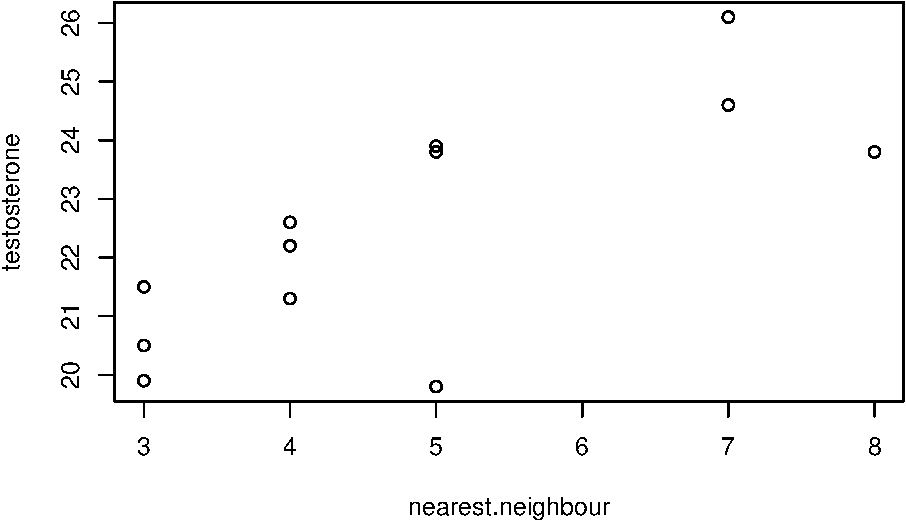
\includegraphics{3rd_Edition_files/figure-latex/unnamed-chunk-5-1.pdf}
\caption{\label{fig:unnamed-chunk-5}Testosterone titre plotted against the distance to the nearest neighbour}
\end{figure}

Not quite publication quality but not bad. You can look at the data and see that there does seem to be a positive relationship between nearest neighbour distance and testosterone level, and you can also see that there aren't any data points that are huge outliers that are likely to have a big effect on your analysis. Now you can go ahead and do some analysis: you want to know if there's a relationship between nearest neighbour distance and testosterone level, so you need to do a correlation analysis. More specifically, you want to know what the correlation coefficient \emph{r} is for the two variables and whether the correlation coefficient is significantly different from zero (see the chapter on correlation for more on this).
Type this in and press enter.

\begin{Shaded}
\begin{Highlighting}[]
\KeywordTok{cor.test}\NormalTok{(nearest.neighbour, testosterone)}

\NormalTok{    Pearson}\StringTok{'s product-moment correlation}

\StringTok{data:  nearest.neighbour and testosterone}
\StringTok{t = 3.62, df = 10, p-value = 0.0047}
\StringTok{alternative hypothesis: true correlation is not equal to 0}
\StringTok{95 percent confidence interval:}
\StringTok{ 0.31635 0.92666}
\StringTok{sample estimates:}
\StringTok{    cor }
\StringTok{0.75346 }
\end{Highlighting}
\end{Shaded}

This has everything you need. It tells you exactly what sort of analysis has been done, and the names of the variables you asked it to analyse. Then you get a significance test and a p-value, telling you that there is a statistically significant correlation between the variables. The last thing in the table is the actual estimate of the correlation coefficient (0.75) and you even get 95\% confidence intervals for the estimate of r.
That's it. You've input your data, drawn a graph and carried out a statistical test. This has hopefully illustrated some important points about how R works to you: you make it do things by typing commands and pressing enter; you can create data objects with your results in; there are commands that make R do things like carry out tests and draw graphs; and at least some of these commands have self-evident names like ``plot''. You've probably also noticed that there seem to be an awful lot of brackets and commas, and you might have found out that if you make mistakes in what you're typing the error messages are rarely helpful. You're halfway there already, but if you want to gain your black belt in command prompt-jitsu you really need to go to the very beginning and start with the basics, which is what the next chapter is all about.

\hypertarget{basics-arithmetic-objects-and-functions}{%
\chapter{Basics: arithmetic, objects and functions}\label{basics-arithmetic-objects-and-functions}}

\hypertarget{arithmetic}{%
\subsection{Arithmetic}\label{arithmetic}}

The simplest way to interact with R is by typing something into the console at the command prompt and pressing enter. If what you've typed makes sense to R it'll do what it's told, if not then you'll get an error message. The simplest things you can get R to do are straightforward sums. Just type in a calculation and press enter.

\begin{Shaded}
\begin{Highlighting}[]
\DecValTok{6}\OperatorTok{+}\DecValTok{3}
\NormalTok{[}\DecValTok{1}\NormalTok{] }\DecValTok{9}
\DecValTok{3}\OperatorTok{^}\DecValTok{3}
\NormalTok{[}\DecValTok{1}\NormalTok{] }\DecValTok{27}
\end{Highlighting}
\end{Shaded}

There are a couple of things to notice here. Firstly, you don't need to type an equals sign -- just hit enter. Secondly, arithmetic operators are mostly the same as in many other packages.

\begin{longtable}[]{@{}ll@{}}
\toprule
Symbol & Does\tabularnewline
\midrule
\endhead
+ & addition\tabularnewline
- & subtraction\tabularnewline
* & multiplication\tabularnewline
/ & division\tabularnewline
\^{} & raised to the power\tabularnewline
\bottomrule
\end{longtable}

Thirdly, why does the answer have a {[}1{]} in front? Because there's only one number in the answer. R is written to be good at dealing not only with single numbers but with groups of numbers: vectors and matrices. When it gives you an answer that contains more than one number it uses numbering like this to indicate where in the group of numbers each answer is. We'll see more of this as we go on.

When you're asking R to do calculations that are more complex than just a single arithmetic operation then it will carry out the calculations in the following order from left to right: first of all calculations in brackets, then exponents, then multiplication and division, then addition and subtraction. When in doubt use brackets to make sure that the calculation that you want to be done is the one that's actually done.

\begin{Shaded}
\begin{Highlighting}[]
\DecValTok{22}\OperatorTok{*}\DecValTok{15}\OperatorTok{+}\DecValTok{6}
\NormalTok{[}\DecValTok{1}\NormalTok{] }\DecValTok{336}
\end{Highlighting}
\end{Shaded}

22 and 15 are multiplied, and then 6 is added to the result of that calculation.

\begin{Shaded}
\begin{Highlighting}[]
\DecValTok{22}\OperatorTok{*}\NormalTok{(}\DecValTok{15}\OperatorTok{+}\DecValTok{6}\NormalTok{)}
\NormalTok{[}\DecValTok{1}\NormalTok{] }\DecValTok{462}
\end{Highlighting}
\end{Shaded}

By adding a pair of brackets we change the order that the calculations are done in: this time 15 and 6 are added together, and 22 is then multiplied by the sum of the two numbers.

\begin{Shaded}
\begin{Highlighting}[]
\DecValTok{22}\OperatorTok{^}\DecValTok{2}\OperatorTok{+}\DecValTok{7}
\NormalTok{[}\DecValTok{1}\NormalTok{] }\DecValTok{491}
\end{Highlighting}
\end{Shaded}

For this calculation 22 is raised to the power 2 and 7 is then added to the result of that calculation.

\begin{Shaded}
\begin{Highlighting}[]
\DecValTok{22}\OperatorTok{^}\NormalTok{(}\DecValTok{2}\OperatorTok{+}\DecValTok{7}\NormalTok{)}
\NormalTok{[}\DecValTok{1}\NormalTok{] }\FloatTok{1.2073e+12}
\end{Highlighting}
\end{Shaded}

By adding a pair of brackets we make sure that the first calculation is to add 2 and 7, and 22 is then raised to the power of the sum of those two numbers. The result of this calculation is a number that's too big for R to display normally, so it's using scientific notation: 1.207e+12 is the way that R expresses 1.207 x 10\^{}12, or 1,207,000,000,000.

You can use multiple brackets, and you can nest your brackets essentially \emph{ad infinitum}.

\begin{Shaded}
\begin{Highlighting}[]
\NormalTok{(}\DecValTok{2}\OperatorTok{*}\NormalTok{(}\FloatTok{17.2}\OperatorTok{+}\DecValTok{5}\NormalTok{))}\OperatorTok{/}\DecValTok{56}
\NormalTok{[}\DecValTok{1}\NormalTok{] }\FloatTok{0.79286}
\end{Highlighting}
\end{Shaded}

\hypertarget{logical-operations}{%
\subsection{Logical operations}\label{logical-operations}}

R doesn't just deal with straightforward arithmetic. You can carry out logical operations as well:

\begin{Shaded}
\begin{Highlighting}[]
\DecValTok{8} \OperatorTok{>}\StringTok{ }\DecValTok{5}
\NormalTok{[}\DecValTok{1}\NormalTok{] }\OtherTok{TRUE}
\end{Highlighting}
\end{Shaded}

returns \texttt{TRUE} whereas

\begin{Shaded}
\begin{Highlighting}[]
\NormalTok{(}\DecValTok{8}\OperatorTok{/}\DecValTok{2}\NormalTok{) }\OperatorTok{>}\StringTok{ }\DecValTok{5}
\NormalTok{[}\DecValTok{1}\NormalTok{] }\OtherTok{FALSE}
\end{Highlighting}
\end{Shaded}

returns \texttt{FALSE}. The full list of logical operators is:

\begin{longtable}[]{@{}ll@{}}
\toprule
\begin{minipage}[b]{0.29\columnwidth}\raggedright
Operator\strut
\end{minipage} & \begin{minipage}[b]{0.65\columnwidth}\raggedright
Test\strut
\end{minipage}\tabularnewline
\midrule
\endhead
\begin{minipage}[t]{0.29\columnwidth}\raggedright
\textgreater{}\strut
\end{minipage} & \begin{minipage}[t]{0.65\columnwidth}\raggedright
Greater than\strut
\end{minipage}\tabularnewline
\begin{minipage}[t]{0.29\columnwidth}\raggedright
\textless{}\strut
\end{minipage} & \begin{minipage}[t]{0.65\columnwidth}\raggedright
Less than\strut
\end{minipage}\tabularnewline
\begin{minipage}[t]{0.29\columnwidth}\raggedright
\textgreater=\strut
\end{minipage} & \begin{minipage}[t]{0.65\columnwidth}\raggedright
Greater than or equal to\strut
\end{minipage}\tabularnewline
\begin{minipage}[t]{0.29\columnwidth}\raggedright
\textless=\strut
\end{minipage} & \begin{minipage}[t]{0.65\columnwidth}\raggedright
Less than or equal to\strut
\end{minipage}\tabularnewline
\begin{minipage}[t]{0.29\columnwidth}\raggedright
==\strut
\end{minipage} & \begin{minipage}[t]{0.65\columnwidth}\raggedright
Exactly equal to. Note this is a double equals sign. Forgetting to use the double equals sign in a logical test is a super-common error.\strut
\end{minipage}\tabularnewline
\begin{minipage}[t]{0.29\columnwidth}\raggedright
!=\strut
\end{minipage} & \begin{minipage}[t]{0.65\columnwidth}\raggedright
Not equal to\strut
\end{minipage}\tabularnewline
\begin{minipage}[t]{0.29\columnwidth}\raggedright
\textbar{}\strut
\end{minipage} & \begin{minipage}[t]{0.65\columnwidth}\raggedright
Or\strut
\end{minipage}\tabularnewline
\begin{minipage}[t]{0.29\columnwidth}\raggedright
\&\strut
\end{minipage} & \begin{minipage}[t]{0.65\columnwidth}\raggedright
And\strut
\end{minipage}\tabularnewline
\bottomrule
\end{longtable}

So

\begin{Shaded}
\begin{Highlighting}[]

\NormalTok{(}\DecValTok{5} \OperatorTok{>}\StringTok{ }\DecValTok{25}\NormalTok{) }\OperatorTok{|}\StringTok{ }\NormalTok{(}\DecValTok{5} \OperatorTok{>}\StringTok{ }\DecValTok{3}\NormalTok{)}
\NormalTok{[}\DecValTok{1}\NormalTok{] }\OtherTok{TRUE}
\end{Highlighting}
\end{Shaded}

Returns \texttt{TRUE} because although 5 is not greater than 25 it is greater than 3, whereas

\begin{Shaded}
\begin{Highlighting}[]
\NormalTok{(}\DecValTok{5} \OperatorTok{>}\StringTok{ }\DecValTok{25}\NormalTok{) }\OperatorTok{&}\StringTok{ }\NormalTok{(}\DecValTok{5} \OperatorTok{>}\StringTok{ }\DecValTok{3}\NormalTok{)}
\NormalTok{[}\DecValTok{1}\NormalTok{] }\OtherTok{FALSE}
\end{Highlighting}
\end{Shaded}

Returns \texttt{FALSE} because now we are asking whether 5 is greater than 25 \textbf{and} 3.

\hypertarget{objects}{%
\subsection{Objects}\label{objects}}

These simple calculations don't produce any kind of output that is remembered by R: the answers appear in the console window but that's all. Sometimes that's OK but a lot of the time we want to store the answer of one of our calculations. The name given to R's ``memory'' is the \textbf{workspace}, and the way to tell R to store something in the workspace is to use something like this:

\begin{Shaded}
\begin{Highlighting}[]
\NormalTok{answer <-}\StringTok{ }\DecValTok{2}\OperatorTok{+}\DecValTok{2}
\end{Highlighting}
\end{Shaded}

Here, we are telling R to add 2+2 and store the answer in an object called \texttt{answer}. Take particular note of the middle symbol, \texttt{\textless{}-}, in the instruction above. This is the \textbf{allocation symbol}, formed of a ``less than'' arrow \texttt{\textless{}} and a hyphen \texttt{-} and it looks like an arrow pointing towards \texttt{answer}. It means ``make the object on the left into the output of the command on the right''. It also works the other way around: 2+2-\textgreater answer.

To find out what is stored in \texttt{answer}, just type its name:

\begin{Shaded}
\begin{Highlighting}[]
\NormalTok{answer}
\NormalTok{[}\DecValTok{1}\NormalTok{] }\DecValTok{4}
\end{Highlighting}
\end{Shaded}

In some older versions of R, and in S-Plus, the underscore character can also be used for allocation, but this is no longer available in recent releases of R. It's useful to know this so that when you try to use someone's old S-Plus code in R you can work out why it doesn't work.

There wasn't an object in the workspace called \texttt{answer} until we ran this code. If there is an allocation to a new name, R will create the new object and store the output of the code to the right of the allocation symbol there. If there is already an object with that name, R will just write the output of the new code to that object, overwriting whatever was stored there in the first place. There is no undo and no ``are you sure'' dialogue box, so be careful.

\begin{Shaded}
\begin{Highlighting}[]
\NormalTok{answer}
\NormalTok{[}\DecValTok{1}\NormalTok{] }\DecValTok{4}
\end{Highlighting}
\end{Shaded}

Our object has the number 4 stored.

\begin{Shaded}
\begin{Highlighting}[]
\NormalTok{answer <-}\StringTok{ }\DecValTok{2}\OperatorTok{*}\DecValTok{3}

\NormalTok{answer}
\NormalTok{[}\DecValTok{1}\NormalTok{] }\DecValTok{6}
\end{Highlighting}
\end{Shaded}

Now it has been overwritten.

You can use objects in calculations in exactly the same way you have already seen numbers being used above.

\begin{Shaded}
\begin{Highlighting}[]
\NormalTok{answer2 <-}\StringTok{ }\NormalTok{(}\FloatTok{3.5}\OperatorTok{+}\DecValTok{1}\NormalTok{)}\OperatorTok{^}\DecValTok{2}
\NormalTok{answer }\OperatorTok{+}\StringTok{ }\NormalTok{answer2}
\NormalTok{[}\DecValTok{1}\NormalTok{] }\FloatTok{26.25}
\end{Highlighting}
\end{Shaded}

You can also store the results of a calculation done with objects as another object.

\begin{Shaded}
\begin{Highlighting}[]
\NormalTok{answer3<-answer}\OperatorTok{/}\NormalTok{answer2}
\NormalTok{answer3}
\NormalTok{[}\DecValTok{1}\NormalTok{] }\FloatTok{0.2963}
\end{Highlighting}
\end{Shaded}

We've already seen that we can do logical operations as well as straightforward arithmetic, and we can store the output of these as objects as well.

\begin{Shaded}
\begin{Highlighting}[]
\NormalTok{test1 <-}\StringTok{ }\NormalTok{answer }\OperatorTok{<}\StringTok{ }\DecValTok{2}
\end{Highlighting}
\end{Shaded}

Asks whether the value stored as the object \texttt{answer} is less than 2, and stores the answer as a new object called test1.

\begin{Shaded}
\begin{Highlighting}[]
\NormalTok{test1}
\NormalTok{[}\DecValTok{1}\NormalTok{] }\OtherTok{FALSE}
\end{Highlighting}
\end{Shaded}

\hypertarget{kinds-of-data}{%
\section{Kinds of data}\label{kinds-of-data}}

So far we have seen examples of R storing two different kinds of data: number, or numerical data, and logical data, stored as \texttt{TRUE} or \texttt{FALSE}. R can also store data as ``Character'' data: strings of letters, numbers or other characters.

\begin{Shaded}
\begin{Highlighting}[]
\NormalTok{name1 <-}\StringTok{ "Steve"}
\end{Highlighting}
\end{Shaded}

Stores the characters that make up the name ``Steve'' as an object calles \texttt{name1}. You'll notice that I put ``Steve'' in inverted commas.\footnote{I am British so I call them ``Inverted commas'' If you're from elsewhere you might call them ``Quote marks''. It's all part of the English language's rich diversity} This is so that R knows that it's character data rather than the name of an object or function.

Numerical data, logical data and character data are all examples of different \textbf{data classes}. R deals with each class differently --- intuitively, you can add numbers together but not letters. If you want to know what a particular object is you can find out using \texttt{class()}:

\begin{Shaded}
\begin{Highlighting}[]
\KeywordTok{class}\NormalTok{(name1)}
\NormalTok{[}\DecValTok{1}\NormalTok{] }\StringTok{"character"}
\end{Highlighting}
\end{Shaded}

Tells us that it is character data. What about \texttt{test1} which we used to store the output from a logical expression?

\begin{Shaded}
\begin{Highlighting}[]
\KeywordTok{class}\NormalTok{(test1)}
\NormalTok{[}\DecValTok{1}\NormalTok{] }\StringTok{"logical"}
\end{Highlighting}
\end{Shaded}

Tells us that it is logical data, which is what we expect. Classes for numerical data can be a little bit more complicated. If you ask the class of an object which is storing a number or numbers it will often simply be \texttt{numeric}, which is straightforward:

\begin{Shaded}
\begin{Highlighting}[]
\KeywordTok{class}\NormalTok{(answer)}
\NormalTok{[}\DecValTok{1}\NormalTok{] }\StringTok{"numeric"}
\end{Highlighting}
\end{Shaded}

You will sometimes see other classes though, including \texttt{integer} if the numbers are all integers, \texttt{double} which means a high-precision number with lots of numbers after the decimal point and \texttt{complex} which refers to a complex number with an imaginary component (if you don't know what this last is, don't worry and stay happy). In practice, these really only matter if you're starting to think about the nitty-gritty of how data are stored in R. R does a good job of converting between the classes in the background if it has to so you don't need to.

One thing to be wary of:

\begin{Shaded}
\begin{Highlighting}[]
\NormalTok{answer}
\NormalTok{[}\DecValTok{1}\NormalTok{] }\DecValTok{6}

\KeywordTok{is.integer}\NormalTok{(answer)}
\NormalTok{[}\DecValTok{1}\NormalTok{] }\OtherTok{FALSE}
\end{Highlighting}
\end{Shaded}

\texttt{answer} is equal to 6, which is an integer, but the is.integer function tells us that it is not. This is because is.integer is telling us about how the number is \emph{stored}, not about what it is, and the number associated with the \texttt{answer} object is not stored as an integer even though it could be. We can change this if we need to:

\begin{Shaded}
\begin{Highlighting}[]
\NormalTok{answer <-}\StringTok{ }\KeywordTok{as.integer}\NormalTok{(answer)}

\KeywordTok{is.integer}\NormalTok{(answer)}
\NormalTok{[}\DecValTok{1}\NormalTok{] }\OtherTok{TRUE}
\end{Highlighting}
\end{Shaded}

\hypertarget{whats-in-my-workspace}{%
\section{What's in my workspace?}\label{whats-in-my-workspace}}

When you first open R, there are no objects stored, but after you've been using it for a while you might have lots. You can get a list of what's in the workspace by using the ls() function (functions are explained in more detail in the next section).

\begin{Shaded}
\begin{Highlighting}[]
\KeywordTok{ls}\NormalTok{()}
\NormalTok{[}\DecValTok{1}\NormalTok{] }\StringTok{"answer"}            \StringTok{"answer2"}           \StringTok{"answer3"}          
\NormalTok{[}\DecValTok{4}\NormalTok{] }\StringTok{"name1"}             \StringTok{"nearest.neighbour"} \StringTok{"test1"}            
\NormalTok{[}\DecValTok{7}\NormalTok{] }\StringTok{"testosterone"}     
\end{Highlighting}
\end{Shaded}

You can remove an object from the workspace by using the rm() function.

\begin{Shaded}
\begin{Highlighting}[]
\KeywordTok{rm}\NormalTok{(answer2)}
\end{Highlighting}
\end{Shaded}

Notice that when you type this, once again it doesn't ask you if you're sure, or give you any other sort of warning, nor does it let you know whether it's done as you asked. The object you asked it to remove has just gone: you can confirm this by using ls() again.

\begin{Shaded}
\begin{Highlighting}[]
\KeywordTok{ls}\NormalTok{()}
\NormalTok{[}\DecValTok{1}\NormalTok{] }\StringTok{"answer"}            \StringTok{"answer3"}           \StringTok{"name1"}            
\NormalTok{[}\DecValTok{4}\NormalTok{] }\StringTok{"nearest.neighbour"} \StringTok{"test1"}             \StringTok{"testosterone"}     
\end{Highlighting}
\end{Shaded}

It's gone, sure enough. If you try to delete an object that doesn't exist you'll get an error message. It's quite common when using R to be pleased when you type in a command and see nothing happen except for the command prompt popping up again. When nothing seems to happen that means that there haven't been any errors, at least as far as R is concerned, which implies that everything has gone smoothly.

R doesn't just store numbers as objects in the workspace******

\hypertarget{functions}{%
\subsection{Functions}\label{functions}}

You can get so far by typing in calculations, but that's obviously not going to be much use for most statistical analyses. Remember that R is not so much a statistical package in the traditional sense, like Minitab, but is really a programming language designed to be good for carrying out statistical analyses. R comes with a huge variety of (mostly) (fairly) short ready-made pieces of code that will do things like manage your data, do more complex mathematical operations on your data, draw graphs and carry out statistical analyses ranging from the simple and straightforward to the eye-wateringly complex. These ready-made pieces of code are called functions. Each function name ends in a pair of round brackets\footnote{See previous comments about the rich diversity of English. ``Brackets'' are what we usually call ``Parentheses'' here in the UK.}, and for many of the more straightforward functions you just type the name of the function and put the name of the object you'd like the procedure carried out on in the brackets.

\begin{Shaded}
\begin{Highlighting}[]
\KeywordTok{log}\NormalTok{(}\DecValTok{27}\NormalTok{)}
\NormalTok{[}\DecValTok{1}\NormalTok{] }\FloatTok{3.2958}
\end{Highlighting}
\end{Shaded}

The natural log of 27

\begin{Shaded}
\begin{Highlighting}[]
\KeywordTok{exp}\NormalTok{(}\DecValTok{3}\NormalTok{)}
\NormalTok{[}\DecValTok{1}\NormalTok{] }\FloatTok{20.086}
\end{Highlighting}
\end{Shaded}

\emph{e} raised to the power 3

\begin{Shaded}
\begin{Highlighting}[]
\KeywordTok{sqrt}\NormalTok{(}\DecValTok{225}\NormalTok{)}
\NormalTok{[}\DecValTok{1}\NormalTok{] }\DecValTok{15}
\end{Highlighting}
\end{Shaded}

Square root of 225

\begin{Shaded}
\begin{Highlighting}[]
\KeywordTok{abs}\NormalTok{(}\OperatorTok{-}\DecValTok{9}\NormalTok{)}
\NormalTok{[}\DecValTok{1}\NormalTok{] }\DecValTok{9}
\end{Highlighting}
\end{Shaded}

Absolute (i.e.~unsigned) value of −9

You can carry out more complex calculations by making the argument of the function (the bit between the brackets) a calculation itself:

\begin{Shaded}
\begin{Highlighting}[]
\KeywordTok{sin}\NormalTok{(}\DecValTok{17}\OperatorTok{+}\NormalTok{answer)}
\end{Highlighting}
\end{Shaded}

will add 17 and whatever the value of the object ``answer'' is, in this case 6, and then calculate the sine of the sum of the two values.

You can use more brackets within the function's brackets to make sure that complicated calculations are carried out in the correct order:

\begin{Shaded}
\begin{Highlighting}[]
\KeywordTok{exp}\NormalTok{((x}\OperatorTok{*}\DecValTok{2}\NormalTok{)}\OperatorTok{^}\NormalTok{(}\DecValTok{1}\OperatorTok{/}\DecValTok{3}\NormalTok{))}
\end{Highlighting}
\end{Shaded}

Will take whatever the value of x is, multiply it by 2, raise it to the power of 1/3 and then calculate the value of \emph{e} raised to the power of that value. In other words, this will calculate \emph{e} to the power of the cube root of 2x).

You can use functions in creating new objects:

\begin{Shaded}
\begin{Highlighting}[]
\NormalTok{D<-}\DecValTok{1}\OperatorTok{/}\KeywordTok{sqrt}\NormalTok{(x)}
\end{Highlighting}
\end{Shaded}

creates an object called ``D'' that has the value of 1 divided by the square root of the value of the object x.

So far we've only looked at functions that have a single argument between the brackets. It's often possible to control specific aspects of the way that the function operates, however, by adding further \textbf{arguments}, separated by commas. These extra arguments serve to do things like modify the way that the function is applied, or tell it to only use part of a dataset, or specify how the function should deal with missing datapoints. Here's a straightforward example. The function \texttt{round()} rounds off a number to a certain number of decimal places. You can tell it the number you want to round off by typing it in between the brackets after the function, and then you can tell it how many decimal places to round to by adding a second argument, \texttt{digits=}, with a comma separating it from the first argument.

\begin{Shaded}
\begin{Highlighting}[]
\KeywordTok{round}\NormalTok{(}\FloatTok{14.5378}\NormalTok{, }\DataTypeTok{digits =} \DecValTok{2}\NormalTok{)}
\NormalTok{[}\DecValTok{1}\NormalTok{] }\FloatTok{14.54}

\KeywordTok{round}\NormalTok{(}\FloatTok{14.5378}\NormalTok{, }\DataTypeTok{digits =} \DecValTok{1}\NormalTok{)}
\NormalTok{[}\DecValTok{1}\NormalTok{] }\FloatTok{14.5}
\end{Highlighting}
\end{Shaded}

Most R functions have default values specified for most of their arguments, and if nothing is specified the function will just use the default value. If we don't define a number of digits for \texttt{round()}, it will assume you want the number rounded off to no decimal places.

\begin{Shaded}
\begin{Highlighting}[]
\KeywordTok{round}\NormalTok{(}\FloatTok{14.5378}\NormalTok{)}
\NormalTok{[}\DecValTok{1}\NormalTok{] }\DecValTok{15}
\end{Highlighting}
\end{Shaded}

A few other examples.

\begin{Shaded}
\begin{Highlighting}[]
\KeywordTok{logb}\NormalTok{(}\DecValTok{27}\NormalTok{, }\DataTypeTok{base=}\FloatTok{3.5}\NormalTok{)}
\NormalTok{[}\DecValTok{1}\NormalTok{] }\FloatTok{2.6309}
\end{Highlighting}
\end{Shaded}

This calculates the logarithm of 27 to the base 3.5. In other words, it calculates the number that 3.5 has to be raised to to get 27.

\begin{Shaded}
\begin{Highlighting}[]
\KeywordTok{signif}\NormalTok{(pi, }\DataTypeTok{digits=}\DecValTok{3}\NormalTok{)}
\NormalTok{[}\DecValTok{1}\NormalTok{] }\FloatTok{3.14}
\KeywordTok{signif}\NormalTok{(pi, }\DataTypeTok{digits=}\DecValTok{5}\NormalTok{)}
\NormalTok{[}\DecValTok{1}\NormalTok{] }\FloatTok{3.1416}
\end{Highlighting}
\end{Shaded}

In this case we specified the arguments precisely. Very often in R the function can work out what the arguments mean simply by their position in the function call, so if you give the \texttt{signif()} function two arguments it assumes that the first is the number to be rounded and the second is the number of signficant digits to round it to.

\begin{Shaded}
\begin{Highlighting}[]
\KeywordTok{signif}\NormalTok{(pi, }\DecValTok{3}\NormalTok{)}
\NormalTok{[}\DecValTok{1}\NormalTok{] }\FloatTok{3.14}
\end{Highlighting}
\end{Shaded}

This can make for less typing but it also makes your code somewhat harder to understand. It's up to you how much you wish to use argument names but I would suggest doing it more often than you might think necessary. It can make things easier when you come to read through the code again.

\hypertarget{exercises}{%
\section{Exercises}\label{exercises}}

\hypertarget{calculations}{%
\subsection{Calculations}\label{calculations}}

Use R to carry out the following calculations (answers are at the end of the chapter if you wish to check):

\begin{itemize}
\item
  3 x 5
\item
  5\^{}2
\item
  Add 8 to 22 and then multiply the answer by 3
\item
  Subtract 2.8 from 12 and then raise the answer to the power of 1.5 plus 1.3924
\item
  Subtract 2.8 from 12, raise the answer to the power of 1.5 and then add 1.3924
\item
  Divide 8 by 2.5 and then divide the answer by 3
\item
  Subtract 2.5 from 8 and then divide the answer by 3
\item
  Divide 2.5 by 3 and subtract the answer from 8
\end{itemize}

\hypertarget{objects-1}{%
\subsection{Objects}\label{objects-1}}

\begin{itemize}
\item
  Create an object called ``X1'' which is the number 73
\item
  Create another object called ``X2'' which is the answer to the sum 101+36
\item
  Multiply X1 and X2 together and store the object as another object called X3
\item
  Subtract 1 from X3 and calculate the 4th root (NB you can calculate the fourth root of a number by raising it to the power of 1/4)
\item
  The answer should be 10
\end{itemize}

\hypertarget{functions-1}{%
\subsection{Functions}\label{functions-1}}

\begin{itemize}
\item
  Calculate the log to the base 10 of x1 using the function \texttt{log10()}
\item
  Calculate the square root of x2 using the function \texttt{sqrt()}
\item
  Calculate the square root of x2 by raising it to the power 0.5: your answer should be the same as when you used the \texttt{sqrt()} function
\item
  use the function \texttt{sum()} to add x1 and x2: you'll need to put both object names inside the brackets and separate them with a comma
\item
  Create an object called ``x4'' which is equal to 67.8953
\item
  The function \texttt{round()} will round a number to a given number of decimal places. The default is zero so start by using this function to round x4 off to zero decimal places
\item
  Now use the round function to give you the value specified by x4 rounded off to three decimal places
\item
  \texttt{floor()} and \texttt{ceiling()} can also be used to trim a number down to an integer: apply both of these functions to x4 and compare the output.
\end{itemize}

\hypertarget{answers-to-exercises}{%
\section{Answers to exercises}\label{answers-to-exercises}}

\hypertarget{calculations-1}{%
\subsection{Calculations}\label{calculations-1}}

\begin{itemize}
\tightlist
\item
  3 x 5
\end{itemize}

\begin{Shaded}
\begin{Highlighting}[]
\DecValTok{3}\OperatorTok{*}\DecValTok{5}
\NormalTok{[}\DecValTok{1}\NormalTok{] }\DecValTok{15}
\end{Highlighting}
\end{Shaded}

\begin{itemize}
\tightlist
\item
  5\^{}2
\end{itemize}

\begin{Shaded}
\begin{Highlighting}[]
\DecValTok{5}\OperatorTok{^}\DecValTok{2}   
\NormalTok{[}\DecValTok{1}\NormalTok{] }\DecValTok{25}
\end{Highlighting}
\end{Shaded}

\begin{itemize}
\tightlist
\item
  Add 8 to 22 and then multiply the answer by 3
\end{itemize}

\begin{Shaded}
\begin{Highlighting}[]
\NormalTok{(}\DecValTok{8}\OperatorTok{+}\DecValTok{22}\NormalTok{)}\OperatorTok{^}\DecValTok{3}
\NormalTok{[}\DecValTok{1}\NormalTok{] }\DecValTok{27000}
\end{Highlighting}
\end{Shaded}

\begin{itemize}
\tightlist
\item
  Subtract 2.8 from 12 and then raise the answer to the power of 1.5 plus 1.3924
\end{itemize}

\begin{Shaded}
\begin{Highlighting}[]
\NormalTok{(}\DecValTok{12}\FloatTok{-2.8}\NormalTok{)}\OperatorTok{^}\NormalTok{(}\FloatTok{1.5+1.3924}\NormalTok{)}
\NormalTok{[}\DecValTok{1}\NormalTok{] }\FloatTok{613.28}
\end{Highlighting}
\end{Shaded}

\begin{itemize}
\tightlist
\item
  Subtract 2.8 from 12, raise the answer to the power of 1.5 and then add 1.3924
\end{itemize}

\begin{Shaded}
\begin{Highlighting}[]
\NormalTok{(}\DecValTok{12}\FloatTok{-2.8}\NormalTok{)}\OperatorTok{^}\FloatTok{1.5+1.3924}
\NormalTok{[}\DecValTok{1}\NormalTok{] }\FloatTok{29.297}
\end{Highlighting}
\end{Shaded}

\begin{itemize}
\tightlist
\item
  Divide 8 by 2.5 and then divide the answer by 3
\end{itemize}

\begin{Shaded}
\begin{Highlighting}[]
\NormalTok{(}\DecValTok{8}\OperatorTok{/}\FloatTok{2.5}\NormalTok{)}\OperatorTok{/}\DecValTok{3}
\NormalTok{[}\DecValTok{1}\NormalTok{] }\FloatTok{1.0667}
\end{Highlighting}
\end{Shaded}

\begin{itemize}
\tightlist
\item
  Subtract 2.5 from 8 and then divide the answer by 3
\end{itemize}

\begin{Shaded}
\begin{Highlighting}[]
\NormalTok{(}\DecValTok{8}\FloatTok{-2.5}\NormalTok{)}\OperatorTok{/}\DecValTok{3}
\NormalTok{[}\DecValTok{1}\NormalTok{] }\FloatTok{1.8333}
\end{Highlighting}
\end{Shaded}

\begin{itemize}
\tightlist
\item
  Divide 2.5 by 3 and subtract the answer from 8
\end{itemize}

\begin{Shaded}
\begin{Highlighting}[]
\DecValTok{8}\FloatTok{-2.5}\OperatorTok{/}\DecValTok{3}       
\NormalTok{[}\DecValTok{1}\NormalTok{] }\FloatTok{7.1667}
\end{Highlighting}
\end{Shaded}

\hypertarget{objects-2}{%
\subsection{Objects}\label{objects-2}}

\begin{itemize}
\tightlist
\item
  Create an object called ``X1'' which is the number 73
\end{itemize}

\begin{Shaded}
\begin{Highlighting}[]
\NormalTok{x1<-}\DecValTok{73}       
\end{Highlighting}
\end{Shaded}

\begin{itemize}
\tightlist
\item
  Create another object called ``X2'' which is the answer to the sum 101+36
\end{itemize}

\begin{Shaded}
\begin{Highlighting}[]
\NormalTok{x2<-}\DecValTok{101}\OperatorTok{+}\DecValTok{36}      
\end{Highlighting}
\end{Shaded}

\begin{itemize}
\tightlist
\item
  Multiply X1 and X2 together and store the object as another object called X3
\end{itemize}

\begin{Shaded}
\begin{Highlighting}[]
\NormalTok{x3<-x1}\OperatorTok{*}\NormalTok{x2    }
\end{Highlighting}
\end{Shaded}

\begin{itemize}
\item
  Subtract 1 from X3 and calculate the 4th root (NB you can calculate the fourth root of a number by raising it to the power of 1/4)
\item
  The answer should be 10
\end{itemize}

\begin{Shaded}
\begin{Highlighting}[]
\NormalTok{(x3}\DecValTok{-1}\NormalTok{)}\OperatorTok{^}\NormalTok{(}\DecValTok{1}\OperatorTok{/}\DecValTok{4}\NormalTok{)}
\NormalTok{[}\DecValTok{1}\NormalTok{] }\DecValTok{10}
\end{Highlighting}
\end{Shaded}

\hypertarget{functions-2}{%
\subsection{Functions}\label{functions-2}}

\begin{itemize}
\tightlist
\item
  Calculate the log to the base 10 of x1 using the function log10()
\end{itemize}

\begin{Shaded}
\begin{Highlighting}[]
\KeywordTok{log10}\NormalTok{(x1)}
\NormalTok{[}\DecValTok{1}\NormalTok{] }\FloatTok{1.8633}
\end{Highlighting}
\end{Shaded}

\begin{itemize}
\tightlist
\item
  Calculate the square root of x2 using the function sqrt()
\end{itemize}

\begin{Shaded}
\begin{Highlighting}[]
\KeywordTok{sqrt}\NormalTok{(x2)}
\NormalTok{[}\DecValTok{1}\NormalTok{] }\FloatTok{11.705}
\end{Highlighting}
\end{Shaded}

\begin{itemize}
\tightlist
\item
  Calculate the square root of x2 by raising it to the power 0.5: your answer should be the same as when you
  used the sqrt() function
\end{itemize}

\begin{Shaded}
\begin{Highlighting}[]
\NormalTok{x2}\OperatorTok{^}\FloatTok{0.5}
\NormalTok{[}\DecValTok{1}\NormalTok{] }\FloatTok{11.705}
\end{Highlighting}
\end{Shaded}

\begin{itemize}
\tightlist
\item
  use the function sum() to add x1 and x2: you'll need to put both object names inside the brackets and
  separate them with a comma
\end{itemize}

\begin{Shaded}
\begin{Highlighting}[]
\KeywordTok{sum}\NormalTok{(x1}\OperatorTok{+}\NormalTok{x2)}
\NormalTok{[}\DecValTok{1}\NormalTok{] }\DecValTok{210}
\end{Highlighting}
\end{Shaded}

\begin{itemize}
\tightlist
\item
  Create an object called ``x4'' which is equal to 67.8953
\end{itemize}

\begin{Shaded}
\begin{Highlighting}[]
\NormalTok{x4<-}\FloatTok{67.8953}
\end{Highlighting}
\end{Shaded}

\begin{itemize}
\tightlist
\item
  The function ``round()'' will round a number to a given number of decimal places. The default is zero so start by using this function to round x4 off to zero decimal places
\end{itemize}

\begin{Shaded}
\begin{Highlighting}[]
\KeywordTok{round}\NormalTok{(x4)}
\NormalTok{[}\DecValTok{1}\NormalTok{] }\DecValTok{68}
\end{Highlighting}
\end{Shaded}

\begin{itemize}
\tightlist
\item
  Now use the round function to give you the value specified by x4 rounded off to three decimal places
\end{itemize}

\begin{Shaded}
\begin{Highlighting}[]
\KeywordTok{round}\NormalTok{(x4,}\DecValTok{3}\NormalTok{)}
\NormalTok{[}\DecValTok{1}\NormalTok{] }\FloatTok{67.895}
\end{Highlighting}
\end{Shaded}

\begin{itemize}
\tightlist
\item
  floor() and ceiling() can also be used to trim a number down to an integer: apply both of these functions to x3 and compare the output.
\end{itemize}

\begin{Shaded}
\begin{Highlighting}[]
\KeywordTok{floor}\NormalTok{(x4)}
\NormalTok{[}\DecValTok{1}\NormalTok{] }\DecValTok{67}
\KeywordTok{ceiling}\NormalTok{(x4)       }
\NormalTok{[}\DecValTok{1}\NormalTok{] }\DecValTok{68}
\end{Highlighting}
\end{Shaded}

\hypertarget{data-vectors-matrices-and-data-frames}{%
\chapter{Data: Vectors, Matrices and Data Frames}\label{data-vectors-matrices-and-data-frames}}

So far we've looked at individual numbers. Interesting data, of course, does not usually consist of simgle numbers, or isolated true/false values: rather, we are likely to be working with lots of data which will be organised into some sort of structure. R is especially good at dealing with objects that are groups of numbers, or groups of character or logical data. In the case of numbers these groups can be can be organised as sequences, which are called vectors\footnote{Vectors of data in R are often referred to as ``atomic vectors''. I'm trying to come up with a witty nuclear-reaction joke about this but I really can't.}, or as two dimensional tables of numbers, which are called matrices (singular matrix). R can also deal with tables that contain more than one kind of data: these are called data frames.

\hypertarget{vectors}{%
\section{Vectors}\label{vectors}}

It's worth spending some time looking at vectors and matrices, because a lot of the things you'll be doing in your analyses involve manipulating sequences and tables of numbers. Let's start by making a vector. The easiest way to do this uses the \texttt{c()} function\footnote{c stands for ``concatenate''. Some people think it means ``combine'' but that's nowhere near as exciting a word.}. If we want a single object containing a series of numbers we can put the numbers as arguments to \texttt{c()} and then assign the output from that to an object.

\begin{Shaded}
\begin{Highlighting}[]
\NormalTok{Y1 <-}\StringTok{ }\KeywordTok{c}\NormalTok{(}\DecValTok{2}\NormalTok{,}\DecValTok{4}\NormalTok{,}\DecValTok{6}\NormalTok{,}\DecValTok{8}\NormalTok{,}\DecValTok{10}\NormalTok{,}\DecValTok{12}\NormalTok{,}\DecValTok{14}\NormalTok{,}\DecValTok{16}\NormalTok{,}\DecValTok{18}\NormalTok{,}\DecValTok{20}\NormalTok{)}
\end{Highlighting}
\end{Shaded}

Here, then, we have created a new object called \texttt{Y1} which is a vector of 10 numbers. Let's have a look at it.

\begin{Shaded}
\begin{Highlighting}[]
\NormalTok{Y1}
\NormalTok{ [}\DecValTok{1}\NormalTok{]  }\DecValTok{2}  \DecValTok{4}  \DecValTok{6}  \DecValTok{8} \DecValTok{10} \DecValTok{12} \DecValTok{14} \DecValTok{16} \DecValTok{18} \DecValTok{20}
\end{Highlighting}
\end{Shaded}

There are many ways to generate vectors of data, and as an example we're going to make another one using a function called \texttt{seq()}, which produces sequences of numbers. The arguments we're using are \texttt{from}, \texttt{to} and \texttt{by}, giving us a function call of \texttt{seq(from=1,\ to=10,\ by=1)}. This means ``make me a sequence of numbers, starting at 1, finishing at 10, and with spacing equal to 1''. We could also write a much shorter command, \texttt{seq(1,\ 10)} because we know that R knows that the first argument between the brackets corresponds to the \texttt{from=} argument, the second one to the \texttt{to=} argument, and the default value for \texttt{by=} is 1, but including the argument names makes everything very clear.

\begin{Shaded}
\begin{Highlighting}[]

\NormalTok{X1 <-}\StringTok{ }\KeywordTok{seq}\NormalTok{(}\DataTypeTok{from=}\DecValTok{1}\NormalTok{, }\DataTypeTok{to=}\DecValTok{10}\NormalTok{, }\DataTypeTok{by=}\DecValTok{1}\NormalTok{)}
\end{Highlighting}
\end{Shaded}

Creates a new object called X1 (a vector in this case) containing a sequence of numbers counting up from 1 to 10. To see what X is just type its name.

\begin{Shaded}
\begin{Highlighting}[]
\NormalTok{X1}
\NormalTok{ [}\DecValTok{1}\NormalTok{]  }\DecValTok{1}  \DecValTok{2}  \DecValTok{3}  \DecValTok{4}  \DecValTok{5}  \DecValTok{6}  \DecValTok{7}  \DecValTok{8}  \DecValTok{9} \DecValTok{10}
\end{Highlighting}
\end{Shaded}

R will quite happily do arithmetic with vectors or matrices as well as simple numbers. What happens when we add a number to a vector?

\begin{Shaded}
\begin{Highlighting}[]
\NormalTok{X1}\OperatorTok{+}\DecValTok{3}
\NormalTok{ [}\DecValTok{1}\NormalTok{]  }\DecValTok{4}  \DecValTok{5}  \DecValTok{6}  \DecValTok{7}  \DecValTok{8}  \DecValTok{9} \DecValTok{10} \DecValTok{11} \DecValTok{12} \DecValTok{13}
\end{Highlighting}
\end{Shaded}

Each number in the vector has 3 added. How about applying a function to a vector?

\begin{Shaded}
\begin{Highlighting}[]
\KeywordTok{log}\NormalTok{(X1)}
\NormalTok{ [}\DecValTok{1}\NormalTok{] }\FloatTok{0.00000} \FloatTok{0.69315} \FloatTok{1.09861} \FloatTok{1.38629} \FloatTok{1.60944} \FloatTok{1.79176} \FloatTok{1.94591} \FloatTok{2.07944} \FloatTok{2.19722}
\NormalTok{[}\DecValTok{10}\NormalTok{] }\FloatTok{2.30259}
\end{Highlighting}
\end{Shaded}

The \texttt{log()} function calculates the natural logarithm, and running it with our X1 vector as an argument gives us a vector with the natural logarithms of the numbers in the original vector. There is an important and powerful point here: when we are using arithmetic, or carrying out logical tests, or using functions which don't summarise sets of numbers in any way, the operation in question is carried out on each number in the vector separately. So

\begin{Shaded}
\begin{Highlighting}[]
\DecValTok{4} \OperatorTok{>}\StringTok{ }\NormalTok{X1}
\NormalTok{ [}\DecValTok{1}\NormalTok{]  }\OtherTok{TRUE}  \OtherTok{TRUE}  \OtherTok{TRUE} \OtherTok{FALSE} \OtherTok{FALSE} \OtherTok{FALSE} \OtherTok{FALSE} \OtherTok{FALSE} \OtherTok{FALSE} \OtherTok{FALSE}
\end{Highlighting}
\end{Shaded}

returns a value of \texttt{TRUE} or \texttt{FALSE} for each member of the vector, rather than a single value. If we were to save the output from this operation as a new object it would be a logical vector of the same length as the original vector which we carried out the operation on.

Some functions return only a single value if we give them a vector as an argument.

\begin{Shaded}
\begin{Highlighting}[]
\KeywordTok{mean}\NormalTok{(X1)}
\NormalTok{[}\DecValTok{1}\NormalTok{] }\FloatTok{5.5}
\end{Highlighting}
\end{Shaded}

gives us the arithmetic mean of all the numbers in the vector, and

\begin{Shaded}
\begin{Highlighting}[]
\KeywordTok{sum}\NormalTok{(X1)}
\NormalTok{[}\DecValTok{1}\NormalTok{] }\DecValTok{55}
\end{Highlighting}
\end{Shaded}

returns the sum of all the numbers in the vector.

We can also do arithmetic with two vectors.

\begin{Shaded}
\begin{Highlighting}[]
\NormalTok{X1 }\OperatorTok{*}\StringTok{ }\NormalTok{Y1}
\NormalTok{ [}\DecValTok{1}\NormalTok{]   }\DecValTok{2}   \DecValTok{8}  \DecValTok{18}  \DecValTok{32}  \DecValTok{50}  \DecValTok{72}  \DecValTok{98} \DecValTok{128} \DecValTok{162} \DecValTok{200}
\NormalTok{Y1 }\OperatorTok{-}\StringTok{ }\NormalTok{X1}
\NormalTok{ [}\DecValTok{1}\NormalTok{]  }\DecValTok{1}  \DecValTok{2}  \DecValTok{3}  \DecValTok{4}  \DecValTok{5}  \DecValTok{6}  \DecValTok{7}  \DecValTok{8}  \DecValTok{9} \DecValTok{10}
\end{Highlighting}
\end{Shaded}

Both of our vectors, X and Y, are the same length in this example, and R just carries out the instruction on each number in the sequence in turn: the first number in X is multiplied by the first number in Y, then the second in X by the second in Y and so on until the last number. What happens if the two vectors are of different lengths? We can set up a vector half as long as X very simply.

\begin{Shaded}
\begin{Highlighting}[]
\NormalTok{X2 <-}\StringTok{ }\KeywordTok{seq}\NormalTok{(}\DecValTok{1}\NormalTok{,}\DecValTok{10}\NormalTok{,}\DecValTok{2}\NormalTok{)}
\NormalTok{X2}
\NormalTok{[}\DecValTok{1}\NormalTok{] }\DecValTok{1} \DecValTok{3} \DecValTok{5} \DecValTok{7} \DecValTok{9}
\end{Highlighting}
\end{Shaded}

Let's add this 5 number vector to our first 10 number vector and see what happens.

\begin{Shaded}
\begin{Highlighting}[]
\NormalTok{X1 }\OperatorTok{+}\StringTok{ }\NormalTok{X2}
\NormalTok{ [}\DecValTok{1}\NormalTok{]  }\DecValTok{2}  \DecValTok{5}  \DecValTok{8} \DecValTok{11} \DecValTok{14}  \DecValTok{7} \DecValTok{10} \DecValTok{13} \DecValTok{16} \DecValTok{19}
\end{Highlighting}
\end{Shaded}

What's happened here? The first number in X (1) has been added to the first number in X2 (1) to give 2. The second numbers in each (2 and 3) have been added in the same way, and so on until we got to the last number in X2, 9, which was added to 5 to give 14. The next number in our answer is 7 - where did that come from? What happens when one vector is shorter than the other is that once all the numbers in the shorter vector have been used, you just start again at the beginning, so the sixth number of X (6) is added to the first number of X2 (1) to give the sixth number in our answer.

1+1=2\\
2+3=5\\
3+5=8\\
4+7=11\\
5+9=14\\
6+1=7\\
7+3=10\\
8+5=13\\
9+7=16\\
10+9=19

This still works if the length of the longer vector is not an exact multiple of the length of the shorter one, but you'll get a warning message.

\begin{Shaded}
\begin{Highlighting}[]
\NormalTok{X3 <-}\StringTok{ }\KeywordTok{seq}\NormalTok{(}\DecValTok{1}\NormalTok{,}\DecValTok{10}\NormalTok{,}\DecValTok{3}\NormalTok{)}
\NormalTok{X3}
\NormalTok{[}\DecValTok{1}\NormalTok{]  }\DecValTok{1}  \DecValTok{4}  \DecValTok{7} \DecValTok{10}
\NormalTok{X1 }\OperatorTok{+}\StringTok{ }\NormalTok{X3}
\NormalTok{ [}\DecValTok{1}\NormalTok{]  }\DecValTok{2}  \DecValTok{6} \DecValTok{10} \DecValTok{14}  \DecValTok{6} \DecValTok{10} \DecValTok{14} \DecValTok{18} \DecValTok{10} \DecValTok{14}
\end{Highlighting}
\end{Shaded}

\hypertarget{matrices}{%
\section{Matrices}\label{matrices}}

When we have data that are arranged in two dimensions rather than one we have a matrix, although not one that features Agent Smith. We can set one up using the \texttt{matrix()} function.

\begin{Shaded}
\begin{Highlighting}[]
\NormalTok{mat1 <-}
\StringTok{  }\KeywordTok{matrix}\NormalTok{(}
    \DataTypeTok{data =} \KeywordTok{seq}\NormalTok{(}\DecValTok{1}\NormalTok{, }\DecValTok{12}\NormalTok{),}
    \DataTypeTok{nrow =} \DecValTok{3}\NormalTok{,}
    \DataTypeTok{ncol =} \DecValTok{4}\NormalTok{,}
    \DataTypeTok{dimnames =} \KeywordTok{list}\NormalTok{(}\KeywordTok{c}\NormalTok{(}\StringTok{"Row 1"}\NormalTok{, }\StringTok{"Row 2"}\NormalTok{, }\StringTok{"Row 3"}\NormalTok{), }
                    \KeywordTok{c}\NormalTok{(}\StringTok{"Col 1"}\NormalTok{, }\StringTok{"Col 2"}\NormalTok{, }\StringTok{"Col 3"}\NormalTok{, }\StringTok{"Col 4"}\NormalTok{))}
\NormalTok{  )}
\end{Highlighting}
\end{Shaded}

This is a complicated looking command. I've kept the argument names in to make it clearer what's going on. We can understand it better by going through each bit in turn.

\begin{Shaded}
\begin{Highlighting}[]
\NormalTok{mat1<-}\StringTok{ }
\end{Highlighting}
\end{Shaded}

Sets up an object called mat1.

\begin{Shaded}
\begin{Highlighting}[]
\KeywordTok{matrix}\NormalTok{(}
  \DataTypeTok{data=}\KeywordTok{seq}\NormalTok{(}\DecValTok{1}\NormalTok{, }\DecValTok{12}\NormalTok{)),}
\end{Highlighting}
\end{Shaded}

The object is a matrix, and the data in the matrix is a sequence of numbers counting from 1 to 12.

\begin{Shaded}
\begin{Highlighting}[]
\NormalTok{nrow=}\DecValTok{3}\NormalTok{, }
\NormalTok{ncol=}\DecValTok{4}\NormalTok{,}
\end{Highlighting}
\end{Shaded}

The number of rows in the matrix is 3 and there are 4 columns.

\begin{Shaded}
\begin{Highlighting}[]
\NormalTok{dimnames=}\KeywordTok{list}\NormalTok{(}\KeywordTok{c}\NormalTok{(}\StringTok{"Row 1"}\NormalTok{,}\StringTok{"Row 2"}\NormalTok{,}\StringTok{"Row 3"}\NormalTok{), }
              \KeywordTok{c}\NormalTok{(}\StringTok{"Col 1"}\NormalTok{,}\StringTok{"Col 2"}\NormalTok{,}\StringTok{"Col 3"}\NormalTok{,}\StringTok{"Col 4"}\NormalTok{))}
\ErrorTok{)}
\end{Highlighting}
\end{Shaded}

This gives the rows and the columns names. We'll talk about lists later on. Let's take a look at our matrix.

\begin{Shaded}
\begin{Highlighting}[]
\NormalTok{mat1}
\NormalTok{      Col }\DecValTok{1}\NormalTok{ Col }\DecValTok{2}\NormalTok{ Col }\DecValTok{3}\NormalTok{ Col }\DecValTok{4}
\NormalTok{Row }\DecValTok{1}     \DecValTok{1}     \DecValTok{4}     \DecValTok{7}    \DecValTok{10}
\NormalTok{Row }\DecValTok{2}     \DecValTok{2}     \DecValTok{5}     \DecValTok{8}    \DecValTok{11}
\NormalTok{Row }\DecValTok{3}     \DecValTok{3}     \DecValTok{6}     \DecValTok{9}    \DecValTok{12}
\end{Highlighting}
\end{Shaded}

Arithmetic and functions which act independently on each member of a vector work in the same way with matrices.

\begin{Shaded}
\begin{Highlighting}[]
\NormalTok{mat2<-mat1}\OperatorTok{/}\DecValTok{3}
\end{Highlighting}
\end{Shaded}

This divides every number in the matrix by three, and allocates the numbers to a new object called ``mat2''.

\begin{Shaded}
\begin{Highlighting}[]
\NormalTok{mat2}
\NormalTok{        Col }\DecValTok{1}\NormalTok{  Col }\DecValTok{2}\NormalTok{  Col }\DecValTok{3}\NormalTok{  Col }\DecValTok{4}
\NormalTok{Row }\DecValTok{1} \FloatTok{0.33333} \FloatTok{1.3333} \FloatTok{2.3333} \FloatTok{3.3333}
\NormalTok{Row }\DecValTok{2} \FloatTok{0.66667} \FloatTok{1.6667} \FloatTok{2.6667} \FloatTok{3.6667}
\NormalTok{Row }\DecValTok{3} \FloatTok{1.00000} \FloatTok{2.0000} \FloatTok{3.0000} \FloatTok{4.0000}
\end{Highlighting}
\end{Shaded}

Here's a second example where we use the \texttt{sqrt()} function to calculate the square root of each value in our matrix.

\begin{Shaded}
\begin{Highlighting}[]
\KeywordTok{sqrt}\NormalTok{(mat1)}
\NormalTok{       Col }\DecValTok{1}\NormalTok{  Col }\DecValTok{2}\NormalTok{  Col }\DecValTok{3}\NormalTok{  Col }\DecValTok{4}
\NormalTok{Row }\DecValTok{1} \FloatTok{1.0000} \FloatTok{2.0000} \FloatTok{2.6458} \FloatTok{3.1623}
\NormalTok{Row }\DecValTok{2} \FloatTok{1.4142} \FloatTok{2.2361} \FloatTok{2.8284} \FloatTok{3.3166}
\NormalTok{Row }\DecValTok{3} \FloatTok{1.7321} \FloatTok{2.4495} \FloatTok{3.0000} \FloatTok{3.4641}
\end{Highlighting}
\end{Shaded}

Functions which return a summary statistic will calculate it on all of the data in the matrix:

\begin{Shaded}
\begin{Highlighting}[]
\KeywordTok{sum}\NormalTok{(mat1)}
\NormalTok{[}\DecValTok{1}\NormalTok{] }\DecValTok{78}
\end{Highlighting}
\end{Shaded}

gives us the sum of all of the numbers in the matrix.

I'm not going to go into the details of how matrices are added and multiplied but I'll just tell you that R will do it without batting an eyelid. Here's an example of R adding two matrices together.

\begin{Shaded}
\begin{Highlighting}[]
\NormalTok{mat3<-}\KeywordTok{matrix}\NormalTok{(}\DataTypeTok{data=}\KeywordTok{seq}\NormalTok{(}\DecValTok{101}\NormalTok{,}\DecValTok{112}\NormalTok{), }\DataTypeTok{nrow=}\DecValTok{3}\NormalTok{, }\DataTypeTok{ncol=}\DecValTok{4}\NormalTok{)}
\end{Highlighting}
\end{Shaded}

This set up a new matrix with the same dimensions as mat1. Let's check it's what we think it is.

\begin{Shaded}
\begin{Highlighting}[]
\NormalTok{mat3}
\NormalTok{     [,}\DecValTok{1}\NormalTok{] [,}\DecValTok{2}\NormalTok{] [,}\DecValTok{3}\NormalTok{] [,}\DecValTok{4}\NormalTok{]}
\NormalTok{[}\DecValTok{1}\NormalTok{,]  }\DecValTok{101}  \DecValTok{104}  \DecValTok{107}  \DecValTok{110}
\NormalTok{[}\DecValTok{2}\NormalTok{,]  }\DecValTok{102}  \DecValTok{105}  \DecValTok{108}  \DecValTok{111}
\NormalTok{[}\DecValTok{3}\NormalTok{,]  }\DecValTok{103}  \DecValTok{106}  \DecValTok{109}  \DecValTok{112}
\end{Highlighting}
\end{Shaded}

Now add them together

\begin{Shaded}
\begin{Highlighting}[]
\NormalTok{mat1}\OperatorTok{+}\NormalTok{mat3}
\NormalTok{      Col }\DecValTok{1}\NormalTok{ Col }\DecValTok{2}\NormalTok{ Col }\DecValTok{3}\NormalTok{ Col }\DecValTok{4}
\NormalTok{Row }\DecValTok{1}   \DecValTok{102}   \DecValTok{108}   \DecValTok{114}   \DecValTok{120}
\NormalTok{Row }\DecValTok{2}   \DecValTok{104}   \DecValTok{110}   \DecValTok{116}   \DecValTok{122}
\NormalTok{Row }\DecValTok{3}   \DecValTok{106}   \DecValTok{112}   \DecValTok{118}   \DecValTok{124}
\end{Highlighting}
\end{Shaded}

\hypertarget{factors-and-data-frames}{%
\section{Factors and Data frames}\label{factors-and-data-frames}}

As we discussed in the last chapter, R data objects can come in a variety of flavours, including as assortment of numeric kinds as well as logical and character. Just in case you need to know you can find out if your vector is numeric using \texttt{mode()} and you can find out what kind of numeric it is using \texttt{class()}.

\begin{Shaded}
\begin{Highlighting}[]
\NormalTok{X1<-}\DecValTok{1}\OperatorTok{:}\DecValTok{12}
\KeywordTok{mode}\NormalTok{(X1)}
\NormalTok{[}\DecValTok{1}\NormalTok{] }\StringTok{"numeric"}
\KeywordTok{class}\NormalTok{(X1)}
\NormalTok{[}\DecValTok{1}\NormalTok{] }\StringTok{"integer"}
\end{Highlighting}
\end{Shaded}

\begin{Shaded}
\begin{Highlighting}[]
\NormalTok{X2<-}\KeywordTok{sqrt}\NormalTok{(X1)}
\KeywordTok{class}\NormalTok{(X2)}
\NormalTok{[}\DecValTok{1}\NormalTok{] }\StringTok{"numeric"}
\end{Highlighting}
\end{Shaded}

R can also cope with strings of characters as objects. These have to be entered with quote marks around them because otherwise R will think that they're the names of objects and return an error when it can't find them.

\begin{Shaded}
\begin{Highlighting}[]
\NormalTok{X1<-}\KeywordTok{c}\NormalTok{(}\StringTok{"Red"}\NormalTok{,}\StringTok{"Red"}\NormalTok{,}\StringTok{"Blue"}\NormalTok{,}\StringTok{"Blue"}\NormalTok{,}\StringTok{"Green"}\NormalTok{)}
\NormalTok{X1}
\NormalTok{[}\DecValTok{1}\NormalTok{] }\StringTok{"Red"}   \StringTok{"Red"}   \StringTok{"Blue"}  \StringTok{"Blue"}  \StringTok{"Green"}
\KeywordTok{mode}\NormalTok{(X1)}
\NormalTok{[}\DecValTok{1}\NormalTok{] }\StringTok{"character"}
\end{Highlighting}
\end{Shaded}

A special type of data in R which we haven't met yet is a \textbf{factor}. When we're collecting data we don't just record numbers: we might record whether a subject is male or female, whether a cricket is winged, wingless or intermediate or whether a leucocyte is an eosinophil, a neutrophil or a basophil. This type of data, where things are divided into classes, is called \textbf{categorical} or \textbf{nominal} data, and in R it is stored as a factor. We can input nominal data into R as numbers if we assign a number to each category, such as 1=red, 2=green and 3=blue and then tell R to make it a factor with the \texttt{factor()} function, but this can lead to confusion. Usually it's better to input data like this as the words themselves as character data and then tell R to make it a factor.

\begin{Shaded}
\begin{Highlighting}[]
\NormalTok{X2<-}\KeywordTok{factor}\NormalTok{(X1)}
\NormalTok{X2}
\NormalTok{[}\DecValTok{1}\NormalTok{] Red   Red   Blue  Blue  Green}
\NormalTok{Levels}\OperatorTok{:}\StringTok{ }\NormalTok{Blue Green Red}
\end{Highlighting}
\end{Shaded}

You can see that now that we have classified X1 as a factor R tells us what the levels are that are found in the factor. Before you start any analysis it's a good idea to check whether you and R are both in agreement over which variables in your data set are factors, because sometimes you will find that you've assumed that something is a factor when it isn't. You can do this with the \texttt{is.factor()} function.

\begin{Shaded}
\begin{Highlighting}[]
\KeywordTok{is.factor}\NormalTok{(X1)}
\NormalTok{[}\DecValTok{1}\NormalTok{] }\OtherTok{FALSE}
\KeywordTok{is.factor}\NormalTok{(X2)}
\NormalTok{[}\DecValTok{1}\NormalTok{] }\OtherTok{TRUE}
\end{Highlighting}
\end{Shaded}

One thing to be aware of is that the \texttt{mode} of a factor will be \texttt{numeric} even if it's coded as characters. This is because R actually recodes variables and assigns a number to each level: you can see the numbers by using the \texttt{as.numeric()} function.

\begin{Shaded}
\begin{Highlighting}[]
\KeywordTok{as.numeric}\NormalTok{(X2)}
\NormalTok{[}\DecValTok{1}\NormalTok{] }\DecValTok{3} \DecValTok{3} \DecValTok{1} \DecValTok{1} \DecValTok{2}
\end{Highlighting}
\end{Shaded}

R codes the factor levels according to their alphabetical order, so ``Blue'' is coded as 1, ``Green'' as 2 and ``Red'' as 3. There's more on this in Chapter 12 when we think about ANOVA, factor levels and summary tables.

It's normal to end up at the end of a study with a table of data that mixes up two or even three different sorts of data. If you've been studying how diet affects whether a species of cricket develops into winged or wingless morphs then for each individual you might have recorded Number (which animal was it) Diet (good or poor), Sex (male or female), Weight (mg), Fat content (mg) and wing morph (winged, wingless or intermediate), giving you a data table looking something like this:

\begin{longtable}[]{@{}lllllll@{}}
\toprule
Number & Diet & Sex & Weight & Fat.content & Morph & Experimenter\tabularnewline
\midrule
\endhead
1 & Poor & M & 156 & 34 & Winged & Jennifer\tabularnewline
2 & Poor & F & 180 & 43 & Winged & Steve\tabularnewline
3 & Good & M & 167 & 40 & Wingless & Ahmed\tabularnewline
4 & Good & F & 190 & 43 & Intermediate & Anna\tabularnewline
\bottomrule
\end{longtable}

Table 3.1 Example cricket data

We could input these data as a series of individual vectors, some numerical and some character, but that would lead to a lot of opportunity for confusion. It's better to keep the whole data table as a single object in R, and there is a special type of object which we can do exactly this with. It's called a \textbf{Data frame}, which is easiest to think of as being like a matrix but with different sorts of data in different columns. Most of the time when you're using real scientific data in R you'll be using a data frame. If you import a data table with multiple data types present then R will automatically classify your data as a data frame. Alternatively, if you want to input your data directly into R you can set up a data frame using the data.frame() function. Here's an example using the cricket data from above.

\begin{Shaded}
\begin{Highlighting}[]
\NormalTok{Number <-}\StringTok{ }\KeywordTok{c}\NormalTok{(}\DecValTok{1}\NormalTok{, }\DecValTok{2}\NormalTok{, }\DecValTok{3}\NormalTok{, }\DecValTok{4}\NormalTok{)}
\NormalTok{Diet <-}\StringTok{ }\KeywordTok{c}\NormalTok{(}\StringTok{"Poor"}\NormalTok{, }\StringTok{"Poor"}\NormalTok{, }\StringTok{"Good"}\NormalTok{, }\StringTok{"Good"}\NormalTok{)}
\NormalTok{Sex <-}\StringTok{ }\KeywordTok{c}\NormalTok{(}\StringTok{"M"}\NormalTok{, }\StringTok{"F"}\NormalTok{, }\StringTok{"M"}\NormalTok{, }\StringTok{"F"}\NormalTok{) }
\NormalTok{Weight <-}\StringTok{ }\KeywordTok{c}\NormalTok{(}\DecValTok{156}\NormalTok{, }\DecValTok{180}\NormalTok{, }\DecValTok{167}\NormalTok{, }\DecValTok{190}\NormalTok{) }
\NormalTok{Fat.content <-}\StringTok{ }\KeywordTok{c}\NormalTok{(}\DecValTok{34}\NormalTok{, }\DecValTok{43}\NormalTok{, }\DecValTok{40}\NormalTok{, }\DecValTok{43}\NormalTok{) }
\NormalTok{Morph <-}\StringTok{ }\KeywordTok{c}\NormalTok{(}\StringTok{"Winged"}\NormalTok{, }\StringTok{"Winged"}\NormalTok{, }\StringTok{"Wingless"}\NormalTok{, }\StringTok{"Intermediate"}\NormalTok{)}
\NormalTok{Experimenter <-}\StringTok{ }\KeywordTok{c}\NormalTok{(}\StringTok{"Jennifer"}\NormalTok{, }\StringTok{"Steve"}\NormalTok{, }\StringTok{"Ahmed"}\NormalTok{, }\StringTok{"Anna"}\NormalTok{)}
       
\NormalTok{crickets <-}\StringTok{ }\KeywordTok{data.frame}\NormalTok{(Number, }
\NormalTok{                       Diet, }
\NormalTok{                       Sex, }
\NormalTok{                       Weight, }
\NormalTok{                       Fat.content, }
\NormalTok{                       Morph, }
\NormalTok{                       Experimenter)}

\KeywordTok{rm}\NormalTok{(Number, Diet, Sex, Weight, Fat.content, Morph, Experimenter)}
\NormalTok{crickets}
\NormalTok{  Number Diet Sex Weight Fat.content        Morph Experimenter}
\DecValTok{1}      \DecValTok{1}\NormalTok{ Poor   M    }\DecValTok{156}          \DecValTok{34}\NormalTok{       Winged     Jennifer}
\DecValTok{2}      \DecValTok{2}\NormalTok{ Poor   F    }\DecValTok{180}          \DecValTok{43}\NormalTok{       Winged        Steve}
\DecValTok{3}      \DecValTok{3}\NormalTok{ Good   M    }\DecValTok{167}          \DecValTok{40}\NormalTok{     Wingless        Ahmed}
\DecValTok{4}      \DecValTok{4}\NormalTok{ Good   F    }\DecValTok{190}          \DecValTok{43}\NormalTok{ Intermediate         Anna}
\end{Highlighting}
\end{Shaded}

What is happening here is that I set up individual vectors for each column of data in our final data frame, and then bind them all together with \texttt{data.frame()}. I then remove all the individual vectors with \texttt{rm()}, leaving just the compund data frame \texttt{crickets}. We can access individual \textbf{variables} within a data frame by writing the name of the data frame, then a \$ symbol, then the name of the variable:

\begin{Shaded}
\begin{Highlighting}[]
\NormalTok{crickets}\OperatorTok{$}\NormalTok{Morph}
\NormalTok{[}\DecValTok{1}\NormalTok{] }\StringTok{"Winged"}       \StringTok{"Winged"}       \StringTok{"Wingless"}     \StringTok{"Intermediate"}
\end{Highlighting}
\end{Shaded}

Note that R assumes that the character vectors that are going into the new data frame are factors and makes them so.

\begin{Shaded}
\begin{Highlighting}[]
\KeywordTok{is.factor}\NormalTok{(crickets}\OperatorTok{$}\NormalTok{Diet)}
\NormalTok{[}\DecValTok{1}\NormalTok{] }\OtherTok{FALSE}
\end{Highlighting}
\end{Shaded}

This isn't necessarily a good thing: for example, we might not want the \texttt{Experimenter} column to be classed as a factor. We can change it back to character data using \texttt{as.character()}, like this:

\begin{Shaded}
\begin{Highlighting}[]
\NormalTok{crickets}\OperatorTok{$}\NormalTok{Experimenter <-}\StringTok{ }\KeywordTok{as.character}\NormalTok{(crickets}\OperatorTok{$}\NormalTok{Experimenter)}

\KeywordTok{is.factor}\NormalTok{(crickets}\OperatorTok{$}\NormalTok{Experimenter)}
\NormalTok{[}\DecValTok{1}\NormalTok{] }\OtherTok{FALSE}
\end{Highlighting}
\end{Shaded}

The function \texttt{str()} (short for structure) is something that is particularly useful with data frames. It tells us the number of rows (observations) of data and the number of columns (variables), then it gives us a list of all the variables in the data frame, what class of variable they are and finally tells you something about their content. If the variable is a factor it tells you how many levels there are, and shows you the first few values for each variable. Let's see what \texttt{str()} gives us from our \texttt{crickets} data frame.

\begin{Shaded}
\begin{Highlighting}[]
\KeywordTok{str}\NormalTok{(crickets)}
\StringTok{'data.frame'}\OperatorTok{:}\StringTok{   }\DecValTok{4}\NormalTok{ obs. of  }\DecValTok{7}\NormalTok{ variables}\OperatorTok{:}
\StringTok{ }\ErrorTok{$}\StringTok{ }\NormalTok{Number      }\OperatorTok{:}\StringTok{ }\NormalTok{num  }\DecValTok{1} \DecValTok{2} \DecValTok{3} \DecValTok{4}
 \OperatorTok{$}\StringTok{ }\NormalTok{Diet        }\OperatorTok{:}\StringTok{ }\NormalTok{chr  }\StringTok{"Poor"} \StringTok{"Poor"} \StringTok{"Good"} \StringTok{"Good"}
 \OperatorTok{$}\StringTok{ }\NormalTok{Sex         }\OperatorTok{:}\StringTok{ }\NormalTok{chr  }\StringTok{"M"} \StringTok{"F"} \StringTok{"M"} \StringTok{"F"}
 \OperatorTok{$}\StringTok{ }\NormalTok{Weight      }\OperatorTok{:}\StringTok{ }\NormalTok{num  }\DecValTok{156} \DecValTok{180} \DecValTok{167} \DecValTok{190}
 \OperatorTok{$}\StringTok{ }\NormalTok{Fat.content }\OperatorTok{:}\StringTok{ }\NormalTok{num  }\DecValTok{34} \DecValTok{43} \DecValTok{40} \DecValTok{43}
 \OperatorTok{$}\StringTok{ }\NormalTok{Morph       }\OperatorTok{:}\StringTok{ }\NormalTok{chr  }\StringTok{"Winged"} \StringTok{"Winged"} \StringTok{"Wingless"} \StringTok{"Intermediate"}
 \OperatorTok{$}\StringTok{ }\NormalTok{Experimenter}\OperatorTok{:}\StringTok{ }\NormalTok{chr  }\StringTok{"Jennifer"} \StringTok{"Steve"} \StringTok{"Ahmed"} \StringTok{"Anna"}
\end{Highlighting}
\end{Shaded}

This is a really good way of checking that everything's OK with your data before you start analysing it. You can see whether all your variables are what you expect them to be, whether all your factors are factors and you can check the size of the data frame. Here you can see that we were successful in changing \texttt{Experimenter} from a factor back to a character variable.

\hypertarget{exercises-1}{%
\section{Exercises}\label{exercises-1}}

\hypertarget{vectors-1}{%
\subsection{Vectors}\label{vectors-1}}

\begin{itemize}
\item
  Check the contents of the workspace using ls(). If they're still there, Delete the objects x1, x2, x3 and x4 that you set up for the previous set of exercises using the rm() function
\item
  Create a vector called ``x1'' consisting of the numbers 1,3,5 and 7
\item
  Create a vector called ``x2'' consisting of the numbers 2,4,6 and 8
\item
  Subtract x1 from x2
\item
  Create a new vector called ``x3'' by multiplying vector x1 by vector x2
\item
  Create a new vector called ``x4'' by taking the square root of each member of x3
\item
  Use the \texttt{mean()} function to calculate the arithmetic mean of the numbers in vector x4
\item
  Use the \texttt{median()} function to calculate the median value of the numbers in vector x3
\end{itemize}

\hypertarget{matrices-1}{%
\subsection{Matrices}\label{matrices-1}}

\begin{itemize}
\item
  Use the \texttt{rm()} function to delete the objects x1, x2, x3, and x4
\item
  Create a new vector called ``V1'' consisting of the following numbers 1,3,5,7,9,11
\item
  Create a matrix called ``mat1'' using the following function: \texttt{mat1\ \textless{}-\ matrix(V1,\ nrow=2)}
\item
  Create a matrix called ``mat2'' using the same function but add an extra argument \texttt{byrow=TRUE}
\item
  Compare the two matrices and note how the data stored in the vector V1 are used to fill up the cells of the two matrices
\end{itemize}

\hypertarget{answers-to-exercises-1}{%
\section{Answers to exercises}\label{answers-to-exercises-1}}

\hypertarget{vectors-2}{%
\subsection{Vectors}\label{vectors-2}}

\begin{itemize}
\tightlist
\item
  Delete the objects x1, x2, x3 and x4 that you set up for the previous set of exercises using the rm() function
\end{itemize}

\begin{Shaded}
\begin{Highlighting}[]
\KeywordTok{rm}\NormalTok{(x1,x2,x3,x4)     }
\end{Highlighting}
\end{Shaded}

\begin{itemize}
\tightlist
\item
  Create a vector called ``x1'' consisting of the numbers 1,3,5 and 7
\end{itemize}

\begin{Shaded}
\begin{Highlighting}[]
\NormalTok{x1 <-}\StringTok{ }\KeywordTok{c}\NormalTok{(}\DecValTok{1}\NormalTok{, }\DecValTok{3}\NormalTok{, }\DecValTok{5}\NormalTok{, }\DecValTok{7}\NormalTok{)}
\end{Highlighting}
\end{Shaded}

\begin{itemize}
\tightlist
\item
  Create a vector called ``x2'' consisting of the numbers 2,4,6 and 8
\end{itemize}

\begin{Shaded}
\begin{Highlighting}[]
\NormalTok{x2 <-}\StringTok{ }\KeywordTok{c}\NormalTok{(}\DecValTok{2}\NormalTok{, }\DecValTok{4}\NormalTok{, }\DecValTok{6}\NormalTok{, }\DecValTok{8}\NormalTok{)}
\end{Highlighting}
\end{Shaded}

\begin{itemize}
\tightlist
\item
  Subtract x1 from x2
\end{itemize}

\begin{Shaded}
\begin{Highlighting}[]
\NormalTok{x2 }\OperatorTok{-}\StringTok{ }\NormalTok{x1}
\NormalTok{[}\DecValTok{1}\NormalTok{] }\DecValTok{1} \DecValTok{1} \DecValTok{1} \DecValTok{1}
\end{Highlighting}
\end{Shaded}

\begin{itemize}
\tightlist
\item
  Create a new vector called ``x3'' by multiplying vector x1 by vector x2
\end{itemize}

\begin{Shaded}
\begin{Highlighting}[]
\NormalTok{x3 <-}\StringTok{ }\NormalTok{x1 }\OperatorTok{*}\StringTok{ }\NormalTok{x2}
\end{Highlighting}
\end{Shaded}

\begin{itemize}
\tightlist
\item
  Create a new vector called ``x4'' by taking the square root of each member of x3
\end{itemize}

\begin{Shaded}
\begin{Highlighting}[]
\NormalTok{x4 <-}\StringTok{ }\KeywordTok{sqrt}\NormalTok{(x3)}
\end{Highlighting}
\end{Shaded}

\begin{itemize}
\tightlist
\item
  Use the mean() function to calculate the arithmetic mean of the numbers in vector x4
\end{itemize}

\begin{Shaded}
\begin{Highlighting}[]
\KeywordTok{mean}\NormalTok{(x4)}
\NormalTok{[}\DecValTok{1}\NormalTok{] }\FloatTok{4.4597}
\end{Highlighting}
\end{Shaded}

\begin{itemize}
\tightlist
\item
  Use the median() function to calculate the median value of the numbers in vector x3
\end{itemize}

\begin{Shaded}
\begin{Highlighting}[]
\KeywordTok{median}\NormalTok{(x3)}
\NormalTok{[}\DecValTok{1}\NormalTok{] }\DecValTok{21}
\end{Highlighting}
\end{Shaded}

\hypertarget{matrices-2}{%
\subsection{Matrices}\label{matrices-2}}

\begin{itemize}
\tightlist
\item
  Use the rm() function to delete the objects x1, x2, x3, x4 and In
\end{itemize}

\begin{Shaded}
\begin{Highlighting}[]
\KeywordTok{rm}\NormalTok{(x1,x2,x3,x4)}
\end{Highlighting}
\end{Shaded}

\begin{itemize}
\tightlist
\item
  Create a new vector called ``V1'' consisting of the following numbers 1,3,5,7,9,11
\end{itemize}

\begin{Shaded}
\begin{Highlighting}[]
\NormalTok{V1<-}\KeywordTok{c}\NormalTok{(}\DecValTok{1}\NormalTok{,}\DecValTok{3}\NormalTok{,}\DecValTok{5}\NormalTok{,}\DecValTok{7}\NormalTok{,}\DecValTok{9}\NormalTok{,}\DecValTok{11}\NormalTok{)}
\end{Highlighting}
\end{Shaded}

\begin{itemize}
\tightlist
\item
  Create a matrix called ``mat1'' using the following function: mat1\textless-matrix(V1,nrow=2)
\end{itemize}

\begin{Shaded}
\begin{Highlighting}[]
\NormalTok{mat1<-}\KeywordTok{matrix}\NormalTok{(V1,}\DataTypeTok{nrow=}\DecValTok{2}\NormalTok{)}
\end{Highlighting}
\end{Shaded}

\begin{itemize}
\tightlist
\item
  Create a matrix called ``mat2'' using the same function but add an extra argument ``byrow=TRUE''
\end{itemize}

\begin{Shaded}
\begin{Highlighting}[]
\NormalTok{mat2<-}\KeywordTok{matrix}\NormalTok{(V1,}\DataTypeTok{nrow=}\DecValTok{2}\NormalTok{,}\DataTypeTok{byrow=}\OtherTok{TRUE}\NormalTok{)}
\end{Highlighting}
\end{Shaded}

\begin{itemize}
\tightlist
\item
  Compare the two matrices and note how the date stored in the vector V1 is used to fill up the cells of the two matrices
\end{itemize}

\begin{Shaded}
\begin{Highlighting}[]
\NormalTok{mat1}
\NormalTok{     [,}\DecValTok{1}\NormalTok{] [,}\DecValTok{2}\NormalTok{] [,}\DecValTok{3}\NormalTok{]}
\NormalTok{[}\DecValTok{1}\NormalTok{,]    }\DecValTok{1}    \DecValTok{5}    \DecValTok{9}
\NormalTok{[}\DecValTok{2}\NormalTok{,]    }\DecValTok{3}    \DecValTok{7}   \DecValTok{11}
\NormalTok{mat2       }
\NormalTok{     [,}\DecValTok{1}\NormalTok{] [,}\DecValTok{2}\NormalTok{] [,}\DecValTok{3}\NormalTok{]}
\NormalTok{[}\DecValTok{1}\NormalTok{,]    }\DecValTok{1}    \DecValTok{3}    \DecValTok{5}
\NormalTok{[}\DecValTok{2}\NormalTok{,]    }\DecValTok{7}    \DecValTok{9}   \DecValTok{11}
\end{Highlighting}
\end{Shaded}

If nothing is specified, the data fill fill up the matrix by column: so row 1, column 1, then row 2 column 1 and so on. If \texttt{byrow\ =\ TRUE} the the data fill the matrix up by row, so row 1 column 1 then row 1 column 2 \&c.

\hypertarget{choosing-data-subscripts-and-subsetting}{%
\chapter{Choosing data: subscripts and subsetting}\label{choosing-data-subscripts-and-subsetting}}

As we saw in the last section, R is set up to deal with data in groups (vectors, matrices and dataframes), and most of the time that you're analysing real data you'll be dealing with data in one of these forms. For some simpler analyses you might be happy just looking at all the data in a particular set of results, but a lot of the time you'll end up thinking ``but what if we exclude males from the analysis?'', or ``does the result hold if we leave out that animal that might have been sick?'' or ``do we still see the trade-off of we only include the plants that flowered?''. All of these can be done quite easily in R, and your chief weapons for such purposes are subscripts, which we'll deal with now, and the \texttt{subset()} command, which we'll talk about once we've dealt with subscripts.

\hypertarget{subscripts}{%
\subsection{Subscripts}\label{subscripts}}

Every number in a vector can be identified by its place in the sequence, and every number in a matrix can be identified by its row and column numbers. You can use subscripts to find individual numbers or groups within data structures. They're remarkably flexible and extremely useful.

\begin{Shaded}
\begin{Highlighting}[]
\NormalTok{Z  <-}\StringTok{  }\KeywordTok{rnorm}\NormalTok{(}\DecValTok{10}\NormalTok{, }\DataTypeTok{mean =} \DecValTok{2}\NormalTok{, }\DataTypeTok{sd =} \FloatTok{0.1}\NormalTok{)}
\end{Highlighting}
\end{Shaded}

This creates a vector called X made up of 10 random numbers drawn from a normal distribution with mean 2 and standard deviation 0.1. NB: if you try to do this your numbers won't be the same as mine, because they're drawn randomly each time.

\begin{Shaded}
\begin{Highlighting}[]
\NormalTok{Z}
\NormalTok{ [}\DecValTok{1}\NormalTok{] }\FloatTok{1.9191} \FloatTok{1.9390} \FloatTok{1.9999} \FloatTok{2.1396} \FloatTok{2.1381} \FloatTok{1.8488} \FloatTok{2.0395} \FloatTok{1.9820} \FloatTok{1.8080} \FloatTok{1.9700}
\end{Highlighting}
\end{Shaded}

If we want to find out what the fifth number in Z is we could just count along until we get there, and when R writes out a vector it helpfully puts a number at the start of each row which tells you where you are in the sequence. In this case we have seven numbers in the first row and the first one is numbered {[}1{]}, then the first number in the second row is numbered {[}8{]}. Just counting along a sequence of numbers can obviously get very unwieldy when we have larger datasets, and the potential for error by the counter is high even with each row being numbered. Fortunately we can just ask what the fifth number is by using a subscript which at its simplest is just a number in square brackets after the name of our vector. R will go and look up whatever's at the position in the vector that corresponds to the number and tell you what it is.

\begin{Shaded}
\begin{Highlighting}[]
\NormalTok{Z[}\DecValTok{5}\NormalTok{]}
\NormalTok{[}\DecValTok{1}\NormalTok{] }\FloatTok{2.1381}
\end{Highlighting}
\end{Shaded}

Subscripts do not have to be single numbers. The subscript can be an object.

\begin{Shaded}
\begin{Highlighting}[]
\NormalTok{p  <-}\StringTok{  }\KeywordTok{c}\NormalTok{(}\DecValTok{2}\NormalTok{, }\DecValTok{5}\NormalTok{, }\DecValTok{7}\NormalTok{)}
\end{Highlighting}
\end{Shaded}

This sets up a new object (\texttt{p}) which is a vector containing three numbers. We can now use this object as a subscript to find out what the second, fifth and seventh numbers in \texttt{Z} are.

\begin{Shaded}
\begin{Highlighting}[]
\NormalTok{Z[p]}
\NormalTok{[}\DecValTok{1}\NormalTok{] }\FloatTok{1.9390} \FloatTok{2.1381} \FloatTok{2.0395}
\end{Highlighting}
\end{Shaded}

The subscript can even be a function.

\begin{Shaded}
\begin{Highlighting}[]
\NormalTok{Z[}\KeywordTok{seq}\NormalTok{(}\DataTypeTok{from =} \DecValTok{1}\NormalTok{, }\DataTypeTok{to =} \DecValTok{5}\NormalTok{, }\DataTypeTok{by =} \DecValTok{2}\NormalTok{)]}
\NormalTok{[}\DecValTok{1}\NormalTok{] }\FloatTok{1.9191} \FloatTok{1.9999} \FloatTok{2.1381}
\end{Highlighting}
\end{Shaded}

We know that seq(from = 1, to = 5, by = 2)) will return the numbers 1, 3 and 5 so here we are asking what the three numbers in \texttt{Z} that occupy those positions are.

The subscript can also ask for the numbers in the vector excluding those specified in the subscript. This is particularly useful if you have some sort of dodgy data point that you want to exclude.

\begin{Shaded}
\begin{Highlighting}[]
\NormalTok{Z[}\OperatorTok{-}\DecValTok{2}\NormalTok{]}
\NormalTok{[}\DecValTok{1}\NormalTok{] }\FloatTok{1.9191} \FloatTok{1.9999} \FloatTok{2.1396} \FloatTok{2.1381} \FloatTok{1.8488} \FloatTok{2.0395} \FloatTok{1.9820} \FloatTok{1.8080} \FloatTok{1.9700}
\end{Highlighting}
\end{Shaded}

This gives us all the numbers in Z except for the second one.

We can include logical expressions in our subscript.

\begin{Shaded}
\begin{Highlighting}[]
\NormalTok{Z[Z}\OperatorTok{>}\FloatTok{1.95}\NormalTok{]}
\NormalTok{[}\DecValTok{1}\NormalTok{] }\FloatTok{1.9999} \FloatTok{2.1396} \FloatTok{2.1381} \FloatTok{2.0395} \FloatTok{1.9820} \FloatTok{1.9700}
\end{Highlighting}
\end{Shaded}

This returns all the numbers in Z that are greater than 1.95.

\begin{Shaded}
\begin{Highlighting}[]
\NormalTok{Z[Z}\OperatorTok{<=}\DecValTok{2}\NormalTok{]}
\NormalTok{[}\DecValTok{1}\NormalTok{] }\FloatTok{1.9191} \FloatTok{1.9390} \FloatTok{1.9999} \FloatTok{1.8488} \FloatTok{1.9820} \FloatTok{1.8080} \FloatTok{1.9700}
\end{Highlighting}
\end{Shaded}

This gives us all the numbers in Z that are less than or equal to 2.

You can use subscripts to find out useful things about your data. If you want to know how many numbers in Z are less than or equal to 2 you can combine some subscripting with the \texttt{length()} command.

\begin{Shaded}
\begin{Highlighting}[]
\KeywordTok{length}\NormalTok{(Z[Z}\OperatorTok{<=}\DecValTok{2}\NormalTok{])}
\NormalTok{[}\DecValTok{1}\NormalTok{] }\DecValTok{7}
\end{Highlighting}
\end{Shaded}

You can calculate other statistics as well. If you want to know the arithmetic mean of the numbers in Z that are less than or equal to 2 you can use a subscript.

\begin{Shaded}
\begin{Highlighting}[]
\KeywordTok{mean}\NormalTok{(Z[Z}\OperatorTok{<=}\DecValTok{2}\NormalTok{])}
\NormalTok{[}\DecValTok{1}\NormalTok{] }\FloatTok{1.9238}
\end{Highlighting}
\end{Shaded}

This approach will work with just about any function. To find out the standard deviation of the same set of numbers use this:

\begin{Shaded}
\begin{Highlighting}[]
\KeywordTok{sd}\NormalTok{(Z[Z}\OperatorTok{<=}\DecValTok{2}\NormalTok{])}
\NormalTok{[}\DecValTok{1}\NormalTok{] }\FloatTok{0.071432}
\end{Highlighting}
\end{Shaded}

and this gives the sum of the numbers in Z that are less than or equal to 2.

\begin{Shaded}
\begin{Highlighting}[]
\KeywordTok{sum}\NormalTok{(Z[Z}\OperatorTok{<=}\DecValTok{2}\NormalTok{])}
\NormalTok{[}\DecValTok{1}\NormalTok{] }\FloatTok{13.467}
\end{Highlighting}
\end{Shaded}

One thing to notice is that using subscripts gives you the values of the numbers that correspond to the criterion\footnote{NB for students: this word is the singular of ``criteria''.} you put in the square brackets but doesn't tell you where in the sequence they are. To do that we can use the function \texttt{which()}. To find out which numbers in Z are less than or equal to 2:

\begin{Shaded}
\begin{Highlighting}[]
\KeywordTok{which}\NormalTok{(Z}\OperatorTok{<=}\DecValTok{2}\NormalTok{)}
\NormalTok{[}\DecValTok{1}\NormalTok{]  }\DecValTok{1}  \DecValTok{2}  \DecValTok{3}  \DecValTok{6}  \DecValTok{8}  \DecValTok{9} \DecValTok{10}
\end{Highlighting}
\end{Shaded}

If we wanted to, we could then use these numbers in a subscript. Here I'm setting up an object that's a vector of these seven numbers.

\begin{Shaded}
\begin{Highlighting}[]
\NormalTok{less.than}\FloatTok{.2}\NormalTok{ <-}\StringTok{ }\KeywordTok{which}\NormalTok{(Z}\OperatorTok{<=}\DecValTok{2}\NormalTok{)}
\end{Highlighting}
\end{Shaded}

Now I can use this object as a subscript itself.

\begin{Shaded}
\begin{Highlighting}[]
\NormalTok{Z[less.than}\FloatTok{.2}\NormalTok{]}
\NormalTok{[}\DecValTok{1}\NormalTok{] }\FloatTok{1.9191} \FloatTok{1.9390} \FloatTok{1.9999} \FloatTok{1.8488} \FloatTok{1.9820} \FloatTok{1.8080} \FloatTok{1.9700}
\end{Highlighting}
\end{Shaded}

The circle is complete. There is actually a serious point to this last part. There are often several different ways of doing the same thing in R. It is often the case that there's an obvious ``best way'', but that isn't always the case: sometimes one way of doing something isn't noticeably easier or better than another, or sometimes doing something one way is better in one situation and doing it another way is better in a different situation. If someone else is doing something differently to you it doesn't necessarily mean that you are wrong: just check what they're doing and have a quick think about which method is better for what you're trying to do. If the answer is ``my method'', or if it's ``I can't see any benefit to using the other method'' then stick with what you're doing.

\hypertarget{boolean-logic-and-more-complex-subscripting}{%
\subsection{Boolean logic and more complex subscripting}\label{boolean-logic-and-more-complex-subscripting}}

R

\hypertarget{subscripts-in-matrices-and-data-frames}{%
\subsection{Subscripts in matrices and data frames}\label{subscripts-in-matrices-and-data-frames}}

Subscripts can also be used to get individual numbers, rows or columns from matrices and data frames in the same way as for vectors, except two numbers are needed to identify an individual cell in these two dimensional data structures. The first number is the row number and the second is the column number. Here's another matrix.

\begin{Shaded}
\begin{Highlighting}[]
\NormalTok{mat4 <-}\StringTok{ }\KeywordTok{matrix}\NormalTok{(}\DataTypeTok{data=}\KeywordTok{seq}\NormalTok{(}\DecValTok{101}\NormalTok{, }\DecValTok{112}\NormalTok{), }\DataTypeTok{nrow=}\DecValTok{3}\NormalTok{, }\DataTypeTok{ncol=}\DecValTok{4}\NormalTok{)}
\NormalTok{mat4}
\NormalTok{     [,}\DecValTok{1}\NormalTok{] [,}\DecValTok{2}\NormalTok{] [,}\DecValTok{3}\NormalTok{] [,}\DecValTok{4}\NormalTok{]}
\NormalTok{[}\DecValTok{1}\NormalTok{,]  }\DecValTok{101}  \DecValTok{104}  \DecValTok{107}  \DecValTok{110}
\NormalTok{[}\DecValTok{2}\NormalTok{,]  }\DecValTok{102}  \DecValTok{105}  \DecValTok{108}  \DecValTok{111}
\NormalTok{[}\DecValTok{3}\NormalTok{,]  }\DecValTok{103}  \DecValTok{106}  \DecValTok{109}  \DecValTok{112}
\end{Highlighting}
\end{Shaded}

To ask ``What's the number that's in the third row and second column of mat2?'', we put the row number first in the subscript, then a comma, then the column number. NB I always have to stop and think about this because I always think it should be column number then row number to make it like xy coordinates.

\begin{Shaded}
\begin{Highlighting}[]
\NormalTok{mat4[}\DecValTok{3}\NormalTok{, }\DecValTok{2}\NormalTok{]}
\NormalTok{[}\DecValTok{1}\NormalTok{] }\DecValTok{106}
\end{Highlighting}
\end{Shaded}

What are the numbers in the third row that are in the second, third and fourth columns?

\begin{Shaded}
\begin{Highlighting}[]
\NormalTok{mat4[}\DecValTok{3}\NormalTok{, }\KeywordTok{c}\NormalTok{(}\DecValTok{2}\NormalTok{, }\DecValTok{3}\NormalTok{, }\DecValTok{4}\NormalTok{)]}
\NormalTok{[}\DecValTok{1}\NormalTok{] }\DecValTok{106} \DecValTok{109} \DecValTok{112}
\end{Highlighting}
\end{Shaded}

To get hold of everything in a particular row, just put the row number followed by a comma and don't put in a number for the column. For example, if you just want the first row of the matrix use a 1.

\begin{Shaded}
\begin{Highlighting}[]
\NormalTok{mat4[}\DecValTok{1}\NormalTok{, ]}
\NormalTok{[}\DecValTok{1}\NormalTok{] }\DecValTok{101} \DecValTok{104} \DecValTok{107} \DecValTok{110}
\end{Highlighting}
\end{Shaded}

Likewise, if you want to get hold of a whole column then leave the row number empty.

\begin{Shaded}
\begin{Highlighting}[]
\NormalTok{mat4[, }\DecValTok{3}\NormalTok{]}
\NormalTok{[}\DecValTok{1}\NormalTok{] }\DecValTok{107} \DecValTok{108} \DecValTok{109}
\end{Highlighting}
\end{Shaded}

This gives us the third column of the matrix

\begin{Shaded}
\begin{Highlighting}[]
\NormalTok{mat4[, }\DecValTok{1}\NormalTok{]}\OperatorTok{+}\NormalTok{mat4[, }\DecValTok{3}\NormalTok{]}
\NormalTok{[}\DecValTok{1}\NormalTok{] }\DecValTok{208} \DecValTok{210} \DecValTok{212}
\end{Highlighting}
\end{Shaded}

This adds the first column of the matrix to the third column.

\hypertarget{subset}{%
\subsection{Subset}\label{subset}}

The \texttt{subset()} function is useful when you want to extract part of a matrix or dataframe. It takes three main arguments, the first being the name of whatever you want to make a subset of, the second is a logical expression and the third tells R which columns you want to choose. It's best to show this with an example. Here's some data that were collected as part of an experiment looking at the effect of environmental temperature on leucocyte count in fish fry.

\begin{Shaded}
\begin{Highlighting}[]
\NormalTok{Counts <-}\StringTok{ }\KeywordTok{read.csv}\NormalTok{(}\StringTok{"Data/Counts.csv"}\NormalTok{, }\DataTypeTok{header=}\NormalTok{T)}
\end{Highlighting}
\end{Shaded}

Let's look at the whole dataset to start with.

\begin{Shaded}
\begin{Highlighting}[]
\NormalTok{Counts}
\NormalTok{  Sex   Temp Weight Count}
\DecValTok{1}\NormalTok{   M  Hot    }\FloatTok{73.25}   \DecValTok{282}
\DecValTok{2}\NormalTok{   M  Hot    }\FloatTok{69.28}   \DecValTok{170}
\DecValTok{3}\NormalTok{   F  Hot    }\FloatTok{81.38}   \DecValTok{151}
\DecValTok{4}\NormalTok{   M  Hot    }\FloatTok{66.07}   \DecValTok{238}
\DecValTok{5}\NormalTok{   F Cold    }\FloatTok{83.32}   \DecValTok{136}
\DecValTok{6}\NormalTok{   F Cold    }\FloatTok{63.06}   \DecValTok{203}
\DecValTok{7}\NormalTok{   M Cold    }\FloatTok{78.48}   \DecValTok{312}
\DecValTok{8}\NormalTok{   M Cold    }\FloatTok{55.38}   \DecValTok{274}
\end{Highlighting}
\end{Shaded}

If we wanted to set up a second data frame containing only data from those fish that weighed 70mg or more, we can just specify the first two arguments.

\begin{Shaded}
\begin{Highlighting}[]
\NormalTok{Counts2 <-}\StringTok{ }\KeywordTok{subset}\NormalTok{(Counts, Weight}\OperatorTok{>=}\DecValTok{70}\NormalTok{)}

\NormalTok{Counts2}
\NormalTok{  Sex   Temp Weight Count}
\DecValTok{1}\NormalTok{   M  Hot    }\FloatTok{73.25}   \DecValTok{282}
\DecValTok{3}\NormalTok{   F  Hot    }\FloatTok{81.38}   \DecValTok{151}
\DecValTok{5}\NormalTok{   F Cold    }\FloatTok{83.32}   \DecValTok{136}
\DecValTok{7}\NormalTok{   M Cold    }\FloatTok{78.48}   \DecValTok{312}
\end{Highlighting}
\end{Shaded}

What if we wanted to extract only the data on weights and leucocyte counts for male fish? For this we use the third argument as well, ``select''.

\begin{Shaded}
\begin{Highlighting}[]
\NormalTok{Counts3 <-}\StringTok{ }\KeywordTok{subset}\NormalTok{(Counts, Sex}\OperatorTok{==}\StringTok{"M"}\NormalTok{, }\DataTypeTok{select=}\KeywordTok{c}\NormalTok{(Weight, Count))}

\NormalTok{Counts3}
\NormalTok{  Weight Count}
\DecValTok{1}  \FloatTok{73.25}   \DecValTok{282}
\DecValTok{2}  \FloatTok{69.28}   \DecValTok{170}
\DecValTok{4}  \FloatTok{66.07}   \DecValTok{238}
\DecValTok{7}  \FloatTok{78.48}   \DecValTok{312}
\DecValTok{8}  \FloatTok{55.38}   \DecValTok{274}
\end{Highlighting}
\end{Shaded}

One thing to notice here is that when we are specifying male fish only in the second argument we use the double equals sign (==). This is what's used in R when we're using logical expressions. The ``M'' is in inverted commas because it's character data. It's easy to forget and use a single equals sign, or miss out the inverted commas. If you do the latter you'll get an error message.

\begin{Shaded}
\begin{Highlighting}[]
\NormalTok{Counts4 <-}\StringTok{ }\KeywordTok{subset}\NormalTok{(Counts, Sex}\OperatorTok{==}\NormalTok{M, }\DataTypeTok{select=}\KeywordTok{c}\NormalTok{(Weight, Count))}
\end{Highlighting}
\end{Shaded}

\texttt{Error\ in\ eval(e,\ x,\ parent.frame())\ :\ object\ \textquotesingle{}M\textquotesingle{}\ not\ found}

If you only put a single equals sign in, however, you won't get an error message. R will ignore the logical expression but it will select the columns specified and your new object will have data from both male and female fish. This could lead to serious errors in your analysis, so always check.

\begin{Shaded}
\begin{Highlighting}[]
\NormalTok{Counts4 <-}\StringTok{ }\KeywordTok{subset}\NormalTok{(Counts, }\DataTypeTok{Sex=}\StringTok{"M"}\NormalTok{, }\DataTypeTok{select=}\KeywordTok{c}\NormalTok{(Weight, Count))}
\end{Highlighting}
\end{Shaded}

See? No error message, but when you look at the output from this command you find that it hasn't been executed in the way you might wish.

\begin{Shaded}
\begin{Highlighting}[]
\NormalTok{Counts4}
\NormalTok{  Weight Count}
\DecValTok{1}  \FloatTok{73.25}   \DecValTok{282}
\DecValTok{2}  \FloatTok{69.28}   \DecValTok{170}
\DecValTok{3}  \FloatTok{81.38}   \DecValTok{151}
\DecValTok{4}  \FloatTok{66.07}   \DecValTok{238}
\DecValTok{5}  \FloatTok{83.32}   \DecValTok{136}
\DecValTok{6}  \FloatTok{63.06}   \DecValTok{203}
\DecValTok{7}  \FloatTok{78.48}   \DecValTok{312}
\DecValTok{8}  \FloatTok{55.38}   \DecValTok{274}
\end{Highlighting}
\end{Shaded}

\texttt{subset()} can also be used within other functions: if, for example, you only want to analyse part of a dataset but you don't want to set up a whole new object. We'll see some examples of this when we look at statistical model fitting in more detail.

\hypertarget{exercises-2}{%
\section{Exercises}\label{exercises-2}}

\hypertarget{subscripts-and-vectors}{%
\subsection{Subscripts and vectors}\label{subscripts-and-vectors}}

\begin{itemize}
\item
  Create a vector called \texttt{x1} containing the numbers 3.6, 3.2, 5.6, 4.9, 6.0, 3.7, 5.5, 4.4 and 4.7.
\item
  Use a subscript to find out the value of the 3rd number in vector x1
\item
  Use a subscript to find out the value of the numbers in vector x1 that aren't in the 5th position
\item
  Add the 1st number in vector x1 to the 6th number in vector x1
\item
  Create a new vector called ``In'' which consists of the numbers 1 and 4
\item
  Use subscripts and the ``In'' vector to calculate the sum of the 1st and 4th numbers in x1
\item
  Calculate the sum of all the numbers in x1 that are less than 4.6
\item
  Calculate the mean of all the numbers in x1 that are greater than or equal to 5
\end{itemize}

\hypertarget{subscripts-and-matrices}{%
\subsection{Subscripts and matrices}\label{subscripts-and-matrices}}

\begin{itemize}
\item
  Generate a matrix called mat1 with 3 rows and 3 columns, using the data from the x1 vector as above. Use the default options for the \texttt{matrix()} function so that the matrix is filled by column.
\item
  Multiply the second value in the first row of mat1 by the third value in the second row of mat1
\item
  Create a new vector called ``V2'' which consists of the numbers in the first row of mat1 added to the numbers in the second row of mat1
\item
  Create a new vector called ``V3'' which consists of the numbers in the second column of mat1 multiplied by the mean of the numbers in the second row of mat1
\item
  Create a new matrix called ``mat3'' which consists of the first row of mat1 as the first column and then the first row of mat2 as the second column. Don't forget that you have to give \texttt{matrix()} a vector of data to fill the new matrix with so you'll have to use the \texttt{c()} function to generate a new vector from the first and third rows of mat1. You can either do this first and create a new object or you can do it within the \texttt{matrix()} function call.
\end{itemize}

\hypertarget{answers-to-exercises-2}{%
\section{Answers to exercises}\label{answers-to-exercises-2}}

\hypertarget{subscripts-and-vectors-1}{%
\subsection{Subscripts and vectors}\label{subscripts-and-vectors-1}}

\begin{itemize}
\tightlist
\item
  Create a vector called \texttt{x1} containing the numbers 3.6, 3.2, 5.6, 4.9, 6.0, 3.7, 5.5, 4.4 and 4.7.
\end{itemize}

\begin{Shaded}
\begin{Highlighting}[]
\NormalTok{x1 <-}\StringTok{ }\KeywordTok{c}\NormalTok{(}\FloatTok{3.6}\NormalTok{, }\FloatTok{3.2}\NormalTok{, }\FloatTok{5.6}\NormalTok{, }\FloatTok{4.9}\NormalTok{, }\FloatTok{6.0}\NormalTok{, }\FloatTok{3.7}\NormalTok{, }\FloatTok{5.5}\NormalTok{, }\FloatTok{4.4}\NormalTok{, }\FloatTok{4.7}\NormalTok{)}
\end{Highlighting}
\end{Shaded}

\begin{itemize}
\tightlist
\item
  Use a subscript to find out the value of the 3rd number in vector x1
\end{itemize}

\begin{Shaded}
\begin{Highlighting}[]
\NormalTok{x1[}\DecValTok{3}\NormalTok{]}
\NormalTok{[}\DecValTok{1}\NormalTok{] }\FloatTok{5.6}
\end{Highlighting}
\end{Shaded}

\begin{itemize}
\tightlist
\item
  Use a subscript to find out the value of the numbers in vector x1 that aren't in the 5th position
\end{itemize}

\begin{Shaded}
\begin{Highlighting}[]
\NormalTok{x1[}\OperatorTok{-}\DecValTok{5}\NormalTok{]}
\NormalTok{[}\DecValTok{1}\NormalTok{] }\FloatTok{3.6} \FloatTok{3.2} \FloatTok{5.6} \FloatTok{4.9} \FloatTok{3.7} \FloatTok{5.5} \FloatTok{4.4} \FloatTok{4.7}
\end{Highlighting}
\end{Shaded}

\begin{itemize}
\tightlist
\item
  Add the 1st number in vector x1 to the 6th number in vector x1
\end{itemize}

\begin{Shaded}
\begin{Highlighting}[]
\CommentTok{#Lots of options for this. Either:}
\NormalTok{x1[}\DecValTok{1}\NormalTok{]}\OperatorTok{+}\NormalTok{x1[}\DecValTok{6}\NormalTok{]}
\NormalTok{[}\DecValTok{1}\NormalTok{] }\FloatTok{7.3}

\CommentTok{#or use the sum() function}
\KeywordTok{sum}\NormalTok{(x1[}\DecValTok{1}\NormalTok{], x1[}\DecValTok{6}\NormalTok{])}
\NormalTok{[}\DecValTok{1}\NormalTok{] }\FloatTok{7.3}

\CommentTok{#or even do it with a new vector that you generate within the subscript}
\KeywordTok{sum}\NormalTok{(x1[}\KeywordTok{c}\NormalTok{(}\DecValTok{1}\NormalTok{,}\DecValTok{6}\NormalTok{)])}
\NormalTok{[}\DecValTok{1}\NormalTok{] }\FloatTok{7.3}
\end{Highlighting}
\end{Shaded}

\begin{itemize}
\tightlist
\item
  Create a new vector called ``In'' which consists of the numbers 1 and 4
\end{itemize}

\begin{Shaded}
\begin{Highlighting}[]
\NormalTok{In <-}\StringTok{ }\KeywordTok{c}\NormalTok{(}\DecValTok{1}\NormalTok{,}\DecValTok{4}\NormalTok{)}
\end{Highlighting}
\end{Shaded}

\begin{itemize}
\tightlist
\item
  Use subscripts and the ``In'' vector to calculate the sum of the 1st and 4th numbers in x1
\end{itemize}

\begin{Shaded}
\begin{Highlighting}[]
\KeywordTok{sum}\NormalTok{(x1[In])}
\NormalTok{[}\DecValTok{1}\NormalTok{] }\FloatTok{8.5}
\end{Highlighting}
\end{Shaded}

\begin{itemize}
\tightlist
\item
  Calculate the sum of all the numbers in x1 that are less than 4.6
\end{itemize}

\begin{Shaded}
\begin{Highlighting}[]
\KeywordTok{sum}\NormalTok{(x1[x1}\OperatorTok{<}\FloatTok{4.6}\NormalTok{])}
\NormalTok{[}\DecValTok{1}\NormalTok{] }\FloatTok{14.9}
\end{Highlighting}
\end{Shaded}

\begin{itemize}
\tightlist
\item
  Calculate the mean of all the numbers in x1 that are greater than or equal to 5
\end{itemize}

\begin{Shaded}
\begin{Highlighting}[]
\KeywordTok{mean}\NormalTok{(x1[x1}\OperatorTok{>=}\DecValTok{5}\NormalTok{])}
\NormalTok{[}\DecValTok{1}\NormalTok{] }\FloatTok{5.7}
\end{Highlighting}
\end{Shaded}

\hypertarget{subscripts-and-matrices-1}{%
\subsection{Subscripts and matrices}\label{subscripts-and-matrices-1}}

\begin{itemize}
\tightlist
\item
  Generate a matrix called mat1 with 3 rows and 3 columns, using the data from the x1 vector as above. Use the default options for the \texttt{matrix()} function so that the matrix is filled by column.
\end{itemize}

\begin{Shaded}
\begin{Highlighting}[]
\NormalTok{mat1 <-}\StringTok{ }\KeywordTok{matrix}\NormalTok{(}\DataTypeTok{data  =}\NormalTok{ x1, }\DataTypeTok{nrow =} \DecValTok{3}\NormalTok{, }\DataTypeTok{ncol =} \DecValTok{3}\NormalTok{)}
\end{Highlighting}
\end{Shaded}

\begin{itemize}
\tightlist
\item
  Multiply the second value in the first row of mat1 by the third value in the second row of mat1
\end{itemize}

\begin{Shaded}
\begin{Highlighting}[]
\NormalTok{mat1[}\DecValTok{1}\NormalTok{,}\DecValTok{2}\NormalTok{] }\OperatorTok{*}\StringTok{ }\NormalTok{mat1[}\DecValTok{2}\NormalTok{,}\DecValTok{3}\NormalTok{]}
\NormalTok{[}\DecValTok{1}\NormalTok{] }\FloatTok{21.56}
\end{Highlighting}
\end{Shaded}

\begin{itemize}
\tightlist
\item
  Create a new vector called ``V2'' which consists of the numbers in the first row of mat1 added to the numbers in the second row of mat1
\end{itemize}

\begin{Shaded}
\begin{Highlighting}[]
\NormalTok{v2 <-}\StringTok{ }\NormalTok{mat1[}\DecValTok{1}\NormalTok{, ] }\OperatorTok{+}\StringTok{ }\NormalTok{mat1[}\DecValTok{2}\NormalTok{, ]}
\NormalTok{v2       }
\NormalTok{[}\DecValTok{1}\NormalTok{]  }\FloatTok{6.8} \FloatTok{10.9}  \FloatTok{9.9}
\end{Highlighting}
\end{Shaded}

\begin{itemize}
\tightlist
\item
  Create a new vector called ``V3'' which consists of the numbers in the second column of mat1 multiplied by the mean of the numbers in the second row of mat1
\end{itemize}

\begin{Shaded}
\begin{Highlighting}[]
\NormalTok{v2 <-}\StringTok{ }\NormalTok{mat1[, }\DecValTok{2}\NormalTok{] }\OperatorTok{*}\StringTok{ }\KeywordTok{mean}\NormalTok{(mat1[}\DecValTok{2}\NormalTok{, ])}
\NormalTok{v2}
\NormalTok{[}\DecValTok{1}\NormalTok{] }\FloatTok{22.213} \FloatTok{27.200} \FloatTok{16.773}
\end{Highlighting}
\end{Shaded}

\begin{itemize}
\tightlist
\item
  Create a new matrix called ``mat3'' which consists of the first row of mat1 as the first column and then the third row of mat1 as the second column
\end{itemize}

\begin{Shaded}
\begin{Highlighting}[]
\CommentTok{# Either generate the new vector of data seperately:}
\NormalTok{v3 <-}\StringTok{ }\KeywordTok{c}\NormalTok{(mat1[}\DecValTok{1}\NormalTok{, ], mat1[}\DecValTok{3}\NormalTok{, ])}
\NormalTok{mat3 <-}\StringTok{ }\KeywordTok{matrix}\NormalTok{(v3, }\DataTypeTok{ncol =} \DecValTok{2}\NormalTok{)        }

\CommentTok{# or do it all in one go within the matrix function.}
\CommentTok{# This is cleaner because you don't end up with a }
\CommentTok{# superfluous object (V3) sitting around in your workspace}
\NormalTok{mat3 <-}\StringTok{ }\KeywordTok{matrix}\NormalTok{(}\KeywordTok{c}\NormalTok{(mat1[}\DecValTok{1}\NormalTok{, ], mat1[}\DecValTok{3}\NormalTok{, ]), }\DataTypeTok{ncol=}\DecValTok{2}\NormalTok{)}


\NormalTok{mat3       }
\NormalTok{     [,}\DecValTok{1}\NormalTok{] [,}\DecValTok{2}\NormalTok{]}
\NormalTok{[}\DecValTok{1}\NormalTok{,]  }\FloatTok{3.6}  \FloatTok{5.6}
\NormalTok{[}\DecValTok{2}\NormalTok{,]  }\FloatTok{4.9}  \FloatTok{3.7}
\NormalTok{[}\DecValTok{3}\NormalTok{,]  }\FloatTok{5.5}  \FloatTok{4.7}
\end{Highlighting}
\end{Shaded}

\hypertarget{r-scripts-and-your-r-workflow}{%
\chapter{R scripts and your R workflow}\label{r-scripts-and-your-r-workflow}}

\hypertarget{writing-and-using-r-scripts}{%
\section{Writing and using R scripts}\label{writing-and-using-r-scripts}}

Up until now we've been thinking about using R simply by typing commands directly into the console. That works, of course, but if you have more than one line of code or if you have long function calls with lots of arguments it can get tricky. Once you're out of the R equivalent of short trousers then it's much better to write your code in a separate editor and then pass the code along to the console when you want it to be run. This brings many benefits:

\begin{itemize}
\tightlist
\item
  If you are writing something with more than about two lines of code there \emph{will} be errors, and it's much easier to fix them in a text editor. Using a script written in a text editor means that if there is a mistake you just fix it and resubmit your code. If there's a mistake in text that you're typing into the console, well you just have to type it all in again, and hope not to make any other mistakes.
\item
  You can edit your code much more easily than you can in a console window. This is quickly going to become important since for almost anything beyond some sorts of basic analysis you'll be using several lines of code, at least. Writing and editing it in a proper editor gives you access to all the features that are there to make it easy to write and edit text. Features like Find \& Replace or Copy \& Paste are universal, but with a decent text editor designed for code you'll also get piles of other goodies. Thes include, amongst others, \emph{syntax highlighting}, whereby the editor colours the different parts of your code to indicate what they are: for example, character strings in green and function names in red; \emph{code folding} which allows you to hide sections of code which you're happy with and focus on the rest; \emph{custom keybindings} so that you can specify particular keystroke combinations to carry out common tasks or insert commonly used pieces of text and \emph{bracket matching} which indicates pairs of brackets or parentheses in your text. The last is especially useful in R because R code can often end up with multiple layers of nested brackets and if one is missing it can take a long time to untangle the mess.
\item
  You can save your script, and then you can come back later and easily replicate your analysis or redraw your graphs. This is hugely important. Really really important. I can't begin to say how important it is. If you don't understand why this is important now, you will.
\item
  You can add \emph{annotations} to your script. These are notes written into the script with a special character which tells R not to pay any attention to them (\texttt{\#}). These are also really really important because when you come to re-run your code sometime after you wrote it it is the annotation which will tell you how it works.
\end{itemize}

Here'as an example of an R script which will download a dataset of monthly counts of UFO reports, originally from the \href{http://www.nuforc.org/}{National UFO Reporting Center} in Eastern Washington State and plot the numbers reported each month since 1900. Don't worry if you don't understand the code, that's not important. The things to notice are that there is syntax highlighting, with different components of the code in different colours and there are comments in the code to explain what it is all doing.

\begin{Shaded}
\begin{Highlighting}[]
\CommentTok{# Script to read data on UFO reports and plot the data since 1900}
\CommentTok{# Audrey Bloggs 25th December 2022}

\CommentTok{# Load data from website}
\NormalTok{UFO <-}\StringTok{ }\KeywordTok{read.csv}\NormalTok{(}\StringTok{"http://www.introductoryr.co.uk/UFO_data.csv"}\NormalTok{,}
                \DataTypeTok{stringsAsFactors =} \OtherTok{FALSE}\NormalTok{)}

\CommentTok{# Convert 'Reports' variable to date}
\NormalTok{UFO}\OperatorTok{$}\NormalTok{Reports <-}\StringTok{ }\KeywordTok{as.Date}\NormalTok{(UFO}\OperatorTok{$}\NormalTok{Reports, }\DataTypeTok{format =} \StringTok{"%d/%m/%Y"}\NormalTok{)}

\CommentTok{# Trim off dates before 1900 which have a different format and convert to NA}
\NormalTok{UFO <-}\StringTok{ }\NormalTok{UFO[}\KeywordTok{which}\NormalTok{((}\OperatorTok{!}\KeywordTok{is.na}\NormalTok{(UFO}\OperatorTok{$}\NormalTok{Reports))), ]}

\CommentTok{# Check the data structure}
\KeywordTok{str}\NormalTok{(UFO)}

\CommentTok{# Plot the data}
\KeywordTok{plot}\NormalTok{(UFO}\OperatorTok{$}\NormalTok{Count }\OperatorTok{~}\StringTok{ }\NormalTok{UFO}\OperatorTok{$}\NormalTok{Reports,}
     \DataTypeTok{type =} \StringTok{'l'}\NormalTok{,}
     \DataTypeTok{col =} \StringTok{"steelblue"}\NormalTok{,}
     \DataTypeTok{xlab =} \StringTok{"Year"}\NormalTok{,}
     \DataTypeTok{ylab =} \StringTok{"Number of UFO reports by month"}\NormalTok{,}
     \DataTypeTok{main  =} \StringTok{"UFO reports by month since 1900"}\NormalTok{)}
\end{Highlighting}
\end{Shaded}

You can run this script yourself. At this point, try just copy-and-pasting the whole lot into the R console. Assuming your computer is connected to the internet it will download the data. You'll see some code and some output in the console window, and it'll draw you a graph that should look like this:

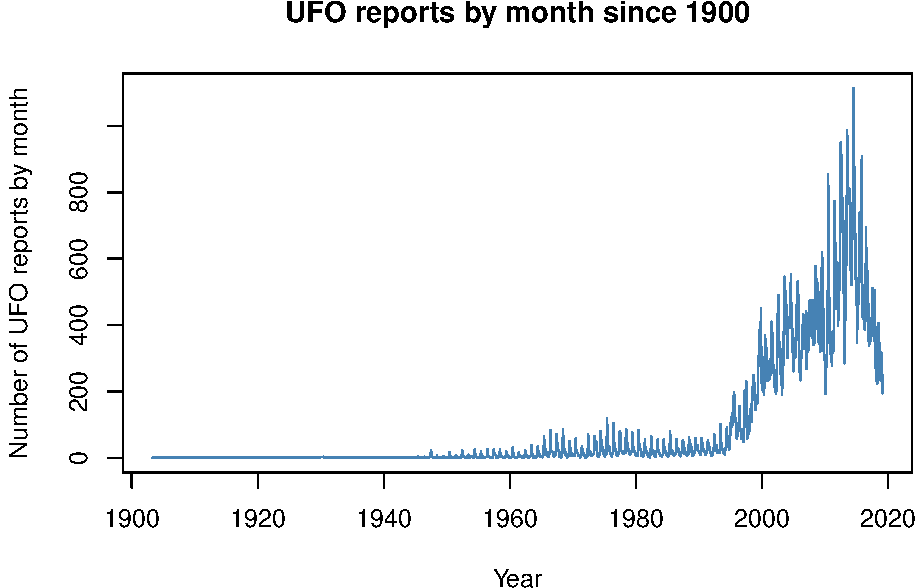
\includegraphics{3rd_Edition_files/figure-latex/unnamed-chunk-163-1.pdf}

\hypertarget{running-code-from-an-r-script-window}{%
\section{Running code from an R script window}\label{running-code-from-an-r-script-window}}

If you want to edit text for an R script you can do a perfectly good job with the built in script editors that ship with the Mac and Windows versions of R. The Mac script editor is good and although it's not a full-featured coding text editor it's very useable. The script editor that comes with the Windows version is a bit basic by comparison with the Mac version but is still perfectly usable. If you don't want to use the built in editors, or if you're using the R on Linux which doesn't have a built-in editor, you can use a basic text editor like Microsoft Notepad, TextEdit which comes with MacOs or Gedit, Nano or any of the other basic editors that come with assorted Linux distros. Hell, you can even use MS Word to edit your R scripts if you must. If you're just starting out and you're not going to be writing long or complex scripts you don't need an all-singing all-dancing professional coding text editor, and for the moment I would recommend the built in script editors because these have the advantage that you can pass code over to the console with a keystroke.

Let's see how to do this using the script for UFO data we saw above. Assuming you're using Windows or a Mac, open a new script window. To open a script editor window on a Mac just select ``New document'' under the ``File'' pull-down menu, or press \texttt{⌘\ N}simultaneously. On a windows machine click ``New script'' under the ``File'' pull down menu. If you've jumped the gun a little and you're using RStudio, pull down the File menu, click on New File and then on R Script. Copy and paste in the code from the example script, or type it in yourself if you prefer. Save it straight away. Put it in a suitable directory (folder) and call it UFOscript. It will be saved with the extension .R indicating that it's an R script, so it will be called UFOscript.R

Now highlight all of the text with your mouse, or select all using a keystroke (\texttt{⌘\ A}on a Mac or Windows-A on a PC). Now, if you're on a Mac, press \texttt{⌘\ enter} together. On a Windows machine, press the Windows key and R together. Your code should appear in the R console window and you should get the plot of UFO sightings over time again. As well as sending the whole script's worth of code in one go, you can highlight smaller blocks of code or individual lines and send them to the console with the same keystrokes.

Now, let's say that you've drawn your plot of UFO sightings, but your friends at UFO club don't want to put the plot in the latest UFO report because they don't like the colour the line is drawn in. You can simply edit your script and run it again to get a new graph. Try changing the word \texttt{steelblue} to \texttt{darkgreen} on the fourth to last line of the script. Make sure the quote marks stay there. Now highlight the block of code beginning with \texttt{plot} and send it to the console again. You should have a new graph with the line of data shown in dark green.

\hypertarget{running-code-from-files-using-source}{%
\section{\texorpdfstring{Running code from files using \texttt{source()}}{Running code from files using source()}}\label{running-code-from-files-using-source}}

You can also run scripts in R directly from a file by using the \texttt{source()} function. You can do this using the \texttt{source()} function and giving the file path to UFOscript.R. On a Mac this might read:

\begin{Shaded}
\begin{Highlighting}[]
\KeywordTok{source}\NormalTok{(}\StringTok{"~/R_scripts/UFOscript.R"}\NormalTok{)}
\end{Highlighting}
\end{Shaded}

if you've put UFOscript.R in a directory called R\_scripts that is in your home directory. On a windows computer it might look like this:

\begin{Shaded}
\begin{Highlighting}[]
\KeywordTok{source}\NormalTok{(}\StringTok{"C:}\CharTok{\textbackslash{}\textbackslash{}}\StringTok{Documents\textbackslash{}R_scripts\textbackslash{}UFOscript.R"}\NormalTok{)}
\end{Highlighting}
\end{Shaded}

if you've put UFOscript.R in a directory called R\_scripts which is itself in a Documents directory on the C: drive.

If you don't know what I mean by a file path, or if you just can't be bothered to type it out, try:

\begin{Shaded}
\begin{Highlighting}[]
\KeywordTok{source}\NormalTok{(}\KeywordTok{file.choose}\NormalTok{())}
\end{Highlighting}
\end{Shaded}

which should give you a mouse clicky dialogue box in which you can navigate to UFOscript.R.

Whichever of the above you choose, you should get the same result. The graph you saw before will be drawn again, but you won't see any code appearing in the console window. This might be what you want, or it might not: as an example, you might want to see the information returned after the \texttt{str()} function call. If you want to see all or part of the code and the output, you have two options. Firstly, adding the argument \texttt{echo\ =\ TRUE} to the \texttt{source()} function call, like this:

\begin{Shaded}
\begin{Highlighting}[]
\KeywordTok{source}\NormalTok{(}\StringTok{"~/R_scripts/UFOscript.R"}\NormalTok{, }\DataTypeTok{echo =} \OtherTok{TRUE}\NormalTok{)}
\end{Highlighting}
\end{Shaded}

will write all the code and the output to the console window, just like when you sent the code straight across from the script window. Alternatively, if you just want some of the code or output, but not all of it, you can use the \texttt{print()} function within your script. Try editing your script so that the line

\begin{Shaded}
\begin{Highlighting}[]
\CommentTok{# Check the data structure}
\KeywordTok{str}\NormalTok{(UFO)}
\end{Highlighting}
\end{Shaded}

now reads:

\begin{Shaded}
\begin{Highlighting}[]
\CommentTok{# Check the data structure}
\KeywordTok{print}\NormalTok{(}\KeywordTok{str}\NormalTok{(UFO))}
\end{Highlighting}
\end{Shaded}

and leave everything else as it was. We've wrapped the \texttt{str(UFO)}, which shows us the \emph{structure} of the \texttt{UFO} object, in the brackets from our \texttt{print()} function. If you save this and \texttt{source()} it you should see that as well as the graph you now get the \texttt{str()} output in the console, but none of the other gubbins.

\hypertarget{workflow-structure-or-what-should-i-put-in-my-script}{%
\section{Workflow structure, or what should I put in my script?}\label{workflow-structure-or-what-should-i-put-in-my-script}}

Let's think a little about \emph{reproducibility}. If you just stick with the popular image of science you might think that it's normal to get some data, run an analysis, quickly bang off a report (or, more likely, use your new analysis to invent a new vaccine overnight) and never look at any of it again. Ask anyone who works in research how often they do this and you're likely to be met with either laughter or incomprehension, and this holds for people working with data in any area, not just science. In my field at least it is normal to find yourself revisiting data and analyses that you haven't looked at for many months or years, and when you do go back to those data you want to be able to reproduce the analysis you did before exactly, and you want to understand what you did and why you did it. It's important, therefore, to be able to reproduce your entire analysis from your script. Ideally, you also want someone else to be able to reproduce your analysis and to understand it --- this might be because you are collaborating with other people, or because you are publishing your research and you want others to be able to reproduce it. This latter is becoming an important concept: what's called \href{https://en.wikipedia.org/wiki/Reproducibility\#Reproducible_research}{reproducible research} is something that originated in computer science but is now establishing itself elsewhere, forexample in ecology as demonstrated by the \href{https://www.britishecologicalsociety.org/}{British Ecological Society}`s \href{https://www.britishecologicalsociety.org/wp-content/uploads/2017/12/guide-to-reproducible-code.pdf}{guide to reproducible code}. You might read this and think that it doesn't apply to you because you're a student who isn't planning to work in research and will never be in the be in the business of inventing new vaccines overnight, or someone who just needs to plot some graphs, but you should still aim for good, reproducible R scripts. If you don't believe me then the first time someone asks you to redraw a graph and make 'just a couple of minor changes' more than a weekend after you made the original then you'll understand.

Assuming that you are analysing data, this would include:

\begin{itemize}
\tightlist
\item
  importing the raw data
\item
  data cleanup if necessary
\item
  exploratory analysis and visualisation
\item
  your final analysis
\item
  final data visualisations which you will put in your report or paper.
\end{itemize}

This way you can reproduce everything just by running your script. Believe me, this is an excellent and simple way to make a reproducible record of your analysis. You might be tempted by alternatives such as saving the workspace with all the objects you've generated and copying bits of code and bits of output into a document, but if done badly this approach can be disastrous and if done well it will be more time consuming than just writing a good script, it will be more complicated and you will find it harder to keep track of all the things that are generated. In case the message isn't clear, write a script.\footnote{See Hurlbert, S.H. (1984) Pseudoreplication and the design of ecological field experiments. Ecological Monographs 54:187--211. \url{http://dx.doi.org/10.2307/1942661} for the classic paper on this.}

\hypertarget{keep-it-neat-making-your-script-easy-to-read}{%
\section{Keep it neat --- making your script easy to read}\label{keep-it-neat-making-your-script-easy-to-read}}

Go online and do a search for ``code writing tips'' or ``best practice for writing code'' and you'll find rather more advice than you might want, and much of it will be written for experienced, hardcore coders. Some of this will have more focus on questions like ``should you put an opening curly bracket on the same line as a fnction definition, or on the next line?,''\footnote{NB for our friends from across the Atlantic: `tarted up': 1. - adj. - wearing an excessive amount of make up, a minimal amount of clothing; ostensibly for the purpose of luring a partner into the act of sexual intercourse. Usually reserved for females, but not as a rule. (www.urbandictionary.com)} and if you are just starting out this might be a little too much. So, here are some basic top tips for writing scripts that aren't horror shows.

\begin{itemize}
\item
  Give your objects sensible names that let you know what they are. This makes it much easier to understand what's going on, especially in long and complicated scripts.
\item
  Be consistent in how you name objects. Remember that R is \emph{case sensitive}, so \texttt{Variable1} is different from \texttt{variable1}. I'd say it's probably best to just stick to lower case all the time to avoid confusion. If you have multiple words in an object name you can separate them using underscores \texttt{my\_variable} or dots \texttt{my.variable}, or camelCase \texttt{myVariable}. If you look on the internet you'll find conflicting views as to which is best: the \href{https://google.github.io/styleguide/Rguide.xml}{Google style guide for R} says not to use underscores and that using dots is preferable, whereas Hadley Wickham's guide in \href{http://adv-r.had.co.nz/Style.html}{Advanced R} recommends using underscores. I'd say that it doesn't really matter which one you use but it's best to pick one and stick with it.
\end{itemize}

\begin{Shaded}
\begin{Highlighting}[]
\NormalTok{UFO <-}\StringTok{ }\KeywordTok{read.csv}\NormalTok{(}\StringTok{"http://www.introductoryr.co.uk/UFO_data.csv"}\NormalTok{,}
                \DataTypeTok{stringsAsFactors =} \OtherTok{FALSE}\NormalTok{)}

\NormalTok{log_ufo_count <-}\StringTok{ }\KeywordTok{log}\NormalTok{(UFO}\OperatorTok{$}\NormalTok{Count)}
\end{Highlighting}
\end{Shaded}

is much better than

\begin{Shaded}
\begin{Highlighting}[]
\NormalTok{data <-}\StringTok{ }\KeywordTok{read.csv}\NormalTok{(}\StringTok{"http://www.introductoryr.co.uk/UFO_data.csv"}\NormalTok{,}
                \DataTypeTok{stringsAsFactors =} \OtherTok{FALSE}\NormalTok{)}

\NormalTok{v1 <-}\StringTok{ }\KeywordTok{log}\NormalTok{(UFO}\OperatorTok{$}\NormalTok{Count)}
\end{Highlighting}
\end{Shaded}

.

\begin{itemize}
\item
  Use plenty of whitespace to make things more readable.
\item
  Write short lines and when your lines are long, spread them over multiple lines and indent them. When you pass R a line of code, it looks to see whether the line it has is cmplete --- whetehr it makes sense in itself as an R instruction. If it is not complete, it will look on the next line and read that, until it either ends up with an instruction that makes sense, or it runs out of lines. If the latter it will prompt you to finish off the code by replacing the \texttt{\textgreater{}} symbol in the console with a \texttt{+}, indicating that it needs some more. I usually see this when I've missed out a closing bracket. Because R has this ability to look for stuff that completes an instruction, you can split function calls over multiple lines. This really makes function calls with lots of arguments much easier to read: I recommend going to a new line every time you have more than two or three arguments to one function call. Here's an example. This will draw the UFO data from before but with a non-parametric smooth line drawn in red.You can see that for the \texttt{plot()} and the \texttt{lines()} functions I've spread the code out over multiple lines, with one argument on each line, and after the first line the remaining lines for each argument are indented, making everything very clear. There is space between each line, making things even clearer.
\end{itemize}

\begin{Shaded}
\begin{Highlighting}[]
\NormalTok{loess_fit <-}\StringTok{ }\KeywordTok{loess}\NormalTok{(UFO}\OperatorTok{$}\NormalTok{Count }\OperatorTok{~}\StringTok{ }\KeywordTok{as.numeric}\NormalTok{(UFO}\OperatorTok{$}\NormalTok{Reports), }\DataTypeTok{span =} \FloatTok{0.2}\NormalTok{)}

\KeywordTok{plot}\NormalTok{(UFO}\OperatorTok{$}\NormalTok{Count }\OperatorTok{~}\StringTok{ }\NormalTok{UFO}\OperatorTok{$}\NormalTok{Reports,}
    \DataTypeTok{col =} \StringTok{"steelblue"}\NormalTok{,}
    \DataTypeTok{type =} \StringTok{"l"}\NormalTok{,}
    \DataTypeTok{xlab =} \StringTok{"Year"}\NormalTok{,}
    \DataTypeTok{ylab =} \StringTok{"UFO reports"}\NormalTok{)}

\KeywordTok{lines}\NormalTok{(UFO}\OperatorTok{$}\NormalTok{Reports, loess_fit}\OperatorTok{$}\NormalTok{fitted,}
      \DataTypeTok{col =} \StringTok{"darkred"}\NormalTok{,}
      \DataTypeTok{lwd =} \DecValTok{2}\NormalTok{)}

\KeywordTok{title}\NormalTok{(}\DataTypeTok{main =} \StringTok{"UFO reports by month since 1900"}\NormalTok{)}
\end{Highlighting}
\end{Shaded}

This code is much easier to read than squashing it all together:

\begin{Shaded}
\begin{Highlighting}[]
\NormalTok{loess_fit <-}\StringTok{ }\KeywordTok{loess}\NormalTok{(UFO}\OperatorTok{$}\NormalTok{Count }\OperatorTok{~}\StringTok{ }\KeywordTok{as.numeric}\NormalTok{(UFO}\OperatorTok{$}\NormalTok{Reports), }\DataTypeTok{span =} \FloatTok{0.2}\NormalTok{)}
\KeywordTok{plot}\NormalTok{(UFO}\OperatorTok{$}\NormalTok{Count }\OperatorTok{~}\StringTok{ }\NormalTok{UFO}\OperatorTok{$}\NormalTok{Reports, }\DataTypeTok{type =} \StringTok{"l"}\NormalTok{, }\DataTypeTok{xlab =} \StringTok{"Year"}\NormalTok{, }\DataTypeTok{ylab =} \StringTok{"UFO reports"}\NormalTok{)}
\KeywordTok{lines}\NormalTok{(UFO}\OperatorTok{$}\NormalTok{Reports, loess_fit}\OperatorTok{$}\NormalTok{fitted, }\DataTypeTok{col =} \StringTok{"darkred"}\NormalTok{, }\DataTypeTok{lwd =} \DecValTok{2}\NormalTok{)}
\KeywordTok{title}\NormalTok{(}\DataTypeTok{main =} \StringTok{"UFO reports by month since 1900"}\NormalTok{)}
\end{Highlighting}
\end{Shaded}

How you do your indenting depends on the particular editor you're using. If you're using the Mac R script editor then you can indent your text using the space bar or the tab key\footnote{Be warned, some people have Very Strong Opinions regarding whether you should use spaces or tabs for indentation. I suppose that it's nice that they have a hobby.}, and then whenever you press enter the text will stay indented until you reach a line where you want to go back to the margin, at which point you can use the delete key to do so. Many coding-oriented text editors, including the RStudio script editor, will automatically indent text for you if you press enter while you're inputting code so long as the code you're putting in isn't a complete instruction. Once it detects that it is it will go back to the margin for you. If you're using some other editors you might have to do your indenting by hand.

\begin{itemize}
\tightlist
\item
  Use spaces. This makes a big difference. Before and after things like \texttt{=} signs, after commas but not before (just like in normal writing), you get the picture I'm sure.
\end{itemize}

\hypertarget{i-wish-i-hadnt-commented-my-code-so-much-said-no-one-ever-4.}{%
\section[``I wish I hadn't commented my code so much'', said no-one, ever.]{\texorpdfstring{``I wish I hadn't commented my code so much'', said no-one, ever.\footnote{Well, hardly anyone, hardly ever.}}{``I wish I hadn't commented my code so much'', said no-one, ever.}}\label{i-wish-i-hadnt-commented-my-code-so-much-said-no-one-ever-4.}}

When you run your code, R will ignore anything on a line that comes after a \#, allowing you to add comments to your script. You can use comments in your script to

\begin{itemize}
\tightlist
\item
  explain what the script does, who wrote it and when,
\item
  divide the script up into logically sensible sections,
\item
  explain to any reader what particular pieces of code do, and
\item
  indicate sections of code which still need work.
\end{itemize}

You can also use commenting to stop particular lines or blocks of code from running, by adding the comment symbol at the start of lines of R code.

You can see an example of commented code in the UFO script above, and here is an example of another script from Audrey with comments.

\begin{Shaded}
\begin{Highlighting}[]
\CommentTok{# Script for generating boxplot of random numbers by 2-level factor}
\CommentTok{# Audrey Bloggs, 31st February 2020}

\CommentTok{#Generate 80 random numbers}
\NormalTok{response <-}\StringTok{ }\KeywordTok{rnorm}\NormalTok{(}\DecValTok{80}\NormalTok{, }\DataTypeTok{mean =} \DecValTok{5}\NormalTok{, }\DataTypeTok{sd =} \DecValTok{1}\NormalTok{)}

\CommentTok{#Generate factor with two levels}
\NormalTok{factor_x <-}\StringTok{ }\KeywordTok{factor}\NormalTok{(}\KeywordTok{rep}\NormalTok{(}\KeywordTok{c}\NormalTok{(}\StringTok{"Red"}\NormalTok{, }\StringTok{"Green"}\NormalTok{), }\DataTypeTok{each =} \DecValTok{40}\NormalTok{))}

\CommentTok{#Draw boxplot using 'plot'}
\CommentTok{#plot(factor_x, response, col = "goldenrod3")}

\CommentTok{#Draw boxplot using 'boxplot'}
\KeywordTok{boxplot}\NormalTok{(response }\OperatorTok{~}\StringTok{ }\NormalTok{factor_x, }
        \DataTypeTok{xlab =} \StringTok{"Factor X"}\NormalTok{,}
        \DataTypeTok{ylab =} \StringTok{"The response"}\NormalTok{,}
        \DataTypeTok{main =} \StringTok{"Responses to factor X"}\NormalTok{,}
        \DataTypeTok{bty =} \StringTok{"l"}\NormalTok{,  }\CommentTok{# Sets box around the plot to bottom and left sides only}
        \DataTypeTok{cex.main =} \FloatTok{0.8}\NormalTok{,  }\CommentTok{# Makes the main title text smaller}
        \DataTypeTok{col =} \StringTok{"goldenrod3"}\NormalTok{)}
\end{Highlighting}
\end{Shaded}

You can see that Audrey has started with a block of commented lines giving some information about the purpose, maker and date of the script, and then we have a comment for each piece of code saying what it does. There is also a line of code which is \emph{commented out}, meaning that it has a \# symbol in front of it and will not run. Finally, if you look at the last piece of code beginning \texttt{boxplot(Y1\textasciitilde{}X1)} you can see that there are some in-line comments to remind the reader what specific arguments to the \texttt{boxplot()} function are doing.

You've probably noticed that Audrey has only added comments to some of the arguments to \texttt{boxplot()}, and has left some others without comments. This is because she doesn't need reminding what \texttt{xlab\ =\ "Factor\ X"} or \texttt{col\ =\ "goldenrod3"} mean, and she's confident that anyone reading her script will know this as well. This leads us on to the question of how detailed you should be in your commenting. If you ask the internet about this you'll get a lot of answers, and you'll come across the idea that `good code is self documenting' --- in other words you should be able to read a script and work out what it's doing without needing much in the way of comments. This is fine for professional coders, and if you are one then that's nice, but if you are only just starting out and still very much on the steep bit of the learning curve then you might need a little more. My philosophy is that you should think about the reader: how much information do you need so that \emph{you} and \emph{anyone else who is likely to read your script} can easily understand it and work out what it does? Intimately familiar with the language and writing code that's only going to be written by other people who know it to a similar degree? Keep your comments to a minimum and let your clean, self-documenting code speak for itself. Just starting out and still having trouble remembering the difference between a vector and a matrix? By all means add as much explanation to your script as \emph{you} need. Equally, if you are a true coding ninja and speak R better than you speak your native language but you are writing a script that will be used by first year students who are new to the language,\footnote{Or for that matter by a senior professor of biochemistry\ldots{}} then you should probably put in a lot more comments than you would normally do so that the people reading and using your script can understand it.

\hypertarget{using-rstudio-to-write-scripts}{%
\section{Using RStudio to write scripts}\label{using-rstudio-to-write-scripts}}

The question of `what text editor should I edit my code in' is something that has given rise to endless debate among programmers\ldots{} to put it mildly. We won't go into the specialist world of text editing software used by professional coders here aside from noting that there are many options, from the über-nerdy \href{http://www.gnu.org/software/emacs/}{Emacs} or \href{http://ex-vi.sourceforge.net/}{vi} through to more recent options such as \href{https://www.sublimetext.com/}{Sublime text}, my personal favourite, or \href{https://github.com/}{GitHub}'s \href{https://atom.io/}{Atom} editor. If you're interested in a third party editor just for R there are many possible options: just Google ``R script editor'' to get more recommendations and opinions than you probably want. \href{http://sourceforge.net/projects/tinn-r/}{TinnR} is popular for Windows users, and there are two more GUI oriented options: \href{https://socialsciences.mcmaster.ca/jfox/Misc/Rcmdr/}{Rcmndr} which actually installs as an R package (more on these later) and \href{https://rkward.kde.org/}{Rkward} on for Linux, Windows or Mac. The \href{https://www.urbandictionary.com/define.php?term=Big\%20Dog}{Big Dog}, however, is \href{https://www.rstudio.com}{RStudio} which has a series of windows including a script editor and a console. The excellent built in script editor and the ease of use of RStudio means that it's very popular nowadays, to the point that we'll devote a whole chapter to an introduction to some of its best features later on.

\hypertarget{help-files-and-packages}{%
\chapter{Help files and packages}\label{help-files-and-packages}}

\hypertarget{using-the-help-files}{%
\section{Using the help files}\label{using-the-help-files}}

When you're using R you can't just pull all the menus down looking for one that has `linear regression' somewhere, like you might do with another piece of software. This means that you will find yourself consulting the help files more than you might do with other packages.
If you know the name of the function you wish to use, you can get the help file by just typing the function name prefixed with a \texttt{?}:

\begin{verbatim}
?cor.test
?log
?glm
\end{verbatim}

This opens a new window with the help file for that command, or if you're using RStudio it will show the help file in the 'help'tab. All the help files follow the same format, and if you're not familiar with the layout they can seem bizarrely incomprehensible. Let's walk through the important bits of the help file for \texttt{cor.test()}:

\begin{verbatim}
cor.test                package:stats                R Documentation
Test for Association/Correlation Between Paired Samples
Description:
     Test for association between paired samples, using one of
     Pearson's product moment correlation coefficient, Kendall's tau or
     Spearman's rho.
\end{verbatim}

This tells you which package it's in (this gets important when you want to do more obscure analysis and have to load new packages), and then tells you what it does. The ``usage'' section\ldots{}

\begin{verbatim}
Usage:
     cor.test(x, ...)
     ## Default S3 method:
     cor.test(x, y,
              alternative = c("two.sided", "less", "greater"),
              method = c("pearson", "kendall", "spearman"),
              exact = NULL, conf.level = 0.95, ...)
     ## S3 method for class 'formula':
     cor.test(formula, data, subset, na.action, ...)
\end{verbatim}

\ldots tells you how to use it. The default method is to type \texttt{cor.test(} and then give the names of the two variables to be tested, separated by commas. There is then a list of the different arguments that can be included in the command. These arguments are followed by some of the possible options, so you can specify \emph{method=``spearman''} if you want a Spearman's r instead of a Pearson. Don't worry about what it means by ``S3 method'' - this refers to the method that R uses to deal with the code and is something that you don't need to concern yourself with if you need to read this book. The next bit then lets you know that you can also use it by inputting a formula. The arguments and their options are then described in a bit more detail:

\begin{verbatim}
Arguments:
    x, y: numeric vectors of data values.  'x' and 'y' must have the
          same length.
alternative: indicates the alternative hypothesis and must be one of
          '"two.sided"', '"greater"' or '"less"'.  You can specify just
          the initial letter.  '"greater"' corresponds to positive
          association, '"less"' to negative association.
  method: a character string indicating which correlation coefficient
          is to be  used for the test.  One of '"pearson"',
          '"kendall"', or '"spearman"', can be abbreviated.
\end{verbatim}

and so on. For each of the arguments there is a line or paragraph telling you what each one does, and in some cases giving a list of what the various options do for that argument. Next up is the section called ``Details''.

\begin{verbatim}
Details

The three methods each estimate the association between paired samples 
and compute a test of the value being zero. They use different measures 
of association, all in the range [-1, 1] with 0 indicating no association. 
These are sometimes referred to as tests of no correlation, but that 
term is often confined to the default method...
\end{verbatim}

This section of the help file gives you some more information about what the function does and how some of the arguments alter the way it works. In the case of \texttt{cor.test()} this is mostly concerned with the specifics of the way that each of the three options available (Pearson's, Spearman's and Kendall's Tau) are calculated.

The next section is called ``Value''.

\begin{verbatim}
Value:
     A list with class '"htest"' containing the following components: 
statistic: the value of the test statistic.
parameter: the degrees of freedom of the test statistic in the case
          that it follows a t distribution.
 p.value: the p-value of the test.
estimate: the estimated measure of association, with name '"cor"',
          '"tau"', or '"rho"' correspoding to the method employed.
\end{verbatim}

This part tells you what the output of the function consists of. If you just tell R to do a \texttt{cor.test()} analysis all of this appears in the console, but if you set up an object containing the output from the test then it is useful to know what information is actually stored there and what it's all called so that you can access it You might not want to do this for a simple correlation analysis, but it gets very useful for more complex analyses because the object will contain handy things like the residuals. When you know what the names of the various pieces of information in the object are you can access them using the object name and a dollar symbol in the same way you can access a variable within a data frame:

\begin{Shaded}
\begin{Highlighting}[]
\NormalTok{obj<-}\KeywordTok{cor.test}\NormalTok{(WeightF, WeightM)}

\NormalTok{obj}\OperatorTok{$}\NormalTok{p.value}
\NormalTok{[}\DecValTok{1}\NormalTok{] }\FloatTok{0.90842}

\NormalTok{obj}\OperatorTok{$}\NormalTok{statistic}
\NormalTok{      t }
\FloatTok{0.11631} 
\end{Highlighting}
\end{Shaded}

The remainder is a couple of references and then an example of how the function might be used. This last is sometimes very useful and sometimes less so. Note that you can just cut and paste the text from the example into the R console window if you want to run the example.

That's all fine if you know what the name of the function is. It's a little like road signs in London though, which are useful so long as you know exactly where you are and how to get to wherever you're going. If you don't know what the name of the function you're after is then you need to search for it, which you can do by using the \texttt{help.search()} function, which will look through the help files for a character string for you.

\begin{Shaded}
\begin{Highlighting}[]
\KeywordTok{help.search}\NormalTok{(}\StringTok{"spearman"}\NormalTok{)}
\end{Highlighting}
\end{Shaded}

will search for things containing ``spearman'' in the help files and will hopefully get you where you want to go. You can also search the help files by just typing a double question mark and then whatever it is you want to search for.

\begin{Shaded}
\begin{Highlighting}[]
\NormalTok{??spearman}
\end{Highlighting}
\end{Shaded}

Will give you the same result as \texttt{help.search("spearman")} and is easier to type.

Unfortunately the search facility sometimes fails to find what you're after, and you'll sometimes have to use other sources: books, manuals, the archives of the R-help mailing list and, if you wish to venture where angels fear to tread, stackoverflow.

\begin{Shaded}
\begin{Highlighting}[]
\KeywordTok{help.search}\NormalTok{(}\StringTok{"Mann-Whitney"}\NormalTok{)}
\end{Highlighting}
\end{Shaded}

\begin{verbatim}
No help files found matching 'Mann-Whitney' using fuzzy matching
\end{verbatim}

\begin{Shaded}
\begin{Highlighting}[]
\KeywordTok{help.search}\NormalTok{(}\StringTok{"Mann.Whitney"}\NormalTok{)}
\end{Highlighting}
\end{Shaded}

\begin{verbatim}
No help files found matching 'Mann-Whitney' using fuzzy matching
\end{verbatim}

\begin{Shaded}
\begin{Highlighting}[]
\KeywordTok{help.search}\NormalTok{(}\StringTok{"mann-whitney"}\NormalTok{)}
\end{Highlighting}
\end{Shaded}

\begin{verbatim}
No help files found matching 'Mann-Whitney' using fuzzy matching
\end{verbatim}

Aaargh! Off to the R-help archives to search for Mann-Whitney

\begin{quote}
From: Jonathan XXXXX
Date: Thu Jan 23 2003 - 13:52:03 EST
On 01/23/03 13:39, Jan YYYYYYY wrote:
\textgreater{} hi,
\textgreater{} i can not find the mann whitney u test in R.
\textgreater{} could someone help me with that ?
See wilcox.test in the ctest package (which loads automatically,
so just say ?wilcox.test)
\end{quote}

So thanks to this person who got made to feel stupid so that I didn't have to.

\hypertarget{packages}{%
\section{Packages}\label{packages}}

The basic R installation comes with a core set of functions that will allow you to do a wide range of analyses and draw a wide variety of graphs. If you want to go further, however, you'll come across one of the best features of R --- the availability of downloadable ``packages'' that load new functions and other objects into your base R installation, enabling you to use an almost infinite range of analysis techniques. Creating a new package is straightforward, and because R is now so widely used in academia the majority of authors of publications describing new analysis techniques release an R package when they publish their new ideas. To give a flavour of how widespread this is, the figure below is a screenshot of part of the contents page from the December 2012 edition of Methods in Ecology and Evolution. The part of the contents page I've focussed on is the ``Applications'' section, is where new statistical techniques tend to get reported in the journal. As you can see, of the seven papers published in this section, five are associated with R packages.

Figure 1. Screenshot of contents table from December 2012 Methods in Ecology and Evolution.

Some packages come with the base installation of R but are not automatically loaded when you start the software. These include:

\begin{itemize}
\tightlist
\item
  \texttt{lattice}, which includes functions for a range of advanced graphics,
\item
  \texttt{MASS}, a package associated with the book ``Modern Applied Statistics with S'' by Venables and Ripley (2002, Springer-Verlag) containing a variety of useful functions to do things like fit generalized linear models with negative binomial errors,
\item
  \texttt{nlme} which lets you fit linear and non-linear mixed-effects models,
\item
  \texttt{cluster} which brings a range of functions for cluster analysis and
\item
  \texttt{survival} which has functions for survival analysis (surprise!).
\end{itemize}

These will already probably be loaded onto your computer, but to make sure you can use the \texttt{installed.packages()} function. Just type it in with nothing between the brackets and you'll get more information about what's there than you really need. If you want to use one of them you can load them into R by using the \texttt{library()} function: so to load the cluster package you just need to type \texttt{library(cluster)} and it will be loaded.

If you want to know a bit more about what's in a particular package you can type \texttt{library(help=PACKAGE)} where \texttt{PACKAGE} is the name of, well, the package. This will get you some information about the package and a list of the various functions that are included in the package. If you want to know more then one of the easiest ways of finding out more information is to go to \url{http://cran.r-project.org/web/packages/available_packages_by_name.html}, which lists all 10000+ packages currently available for R. If you click on the name of a package you'll be able to navigate to a link for the package manual which should tell you everything you might ever want to know. It might be difficult to follow if you're a biologist because it's likely to be written for consumption by statisticians, but you'll just need to persevere.

Most of the R packages out there aren't installed on your machine by default, of course. Let's say you're a community ecologist and you want to use the \texttt{vegan} package, which codes for a wide variety of functions to do things like calculate diversity indices and carry out ordinations. If you look on CRAN you can find the web page for vegan at \url{http://cran.r-project.org/web/packages/vegan/index.html}, which lets you look at the manual for the package and also provides links to a number of ``vignettes'' - documents giving details of how to carry out specific analyses using the package. These can be very useful once you've got the package installed: when it's three o'clock in the morning and you're so desperate you would sell your cat's soul to Satan just to get that NMDS done those vignettes can preserve your sanity, but there's nothing obvious on the web page that you can click on to actually install it on your computer.

What you need to know before you install a package is that the central repository for R stuff, CRAN (Comprehensive R Archive Network) has a series of mirror sites around the World. When you download something you should choose a mirror site near to you so that you can avoid overloading the main CRAN site. A list of CRAN mirrors is available at \url{http://cran.r-project.org/mirrors.html}. Take a look at it and find some mirror sites near where you are.

Now that you've got an idea of which mirror sites you might want to use, you can set a mirror site by using \texttt{chooseCRANmirror()}, which will bring up a window that lets you choose the mirror site you'd like to use, and then you can install the package using the \texttt{install.packages()} function.

\begin{Shaded}
\begin{Highlighting}[]
\KeywordTok{install.packages}\NormalTok{(}\StringTok{"vegan"}\NormalTok{)}
\end{Highlighting}
\end{Shaded}

\begin{verbatim}
also installing the dependency ‘permute’
trying URL 'http://www.stats.bris.ac.uk/R/bin/macosx/leopard/contrib/2.15/permute_0.7-0.tgz'
Content type 'application/x-gzip' length 220346 bytes (215 Kb)
opened URL
==================================================
downloaded 215 Kb

trying URL 'http://www.stats.bris.ac.uk/R/bin/macosx/leopard/contrib/2.15/vegan_2.0-5.tgz'
Content type 'application/x-gzip' length 2353906 bytes (2.2 Mb)
opened URL
==================================================
downloaded 2.2 Mb


The downloaded binary packages are in
  /var/folders/qm/_szqszq95c34jn73g8b03bbh0000gn/T//Rtmpm0BWXn/downloaded_packages
\end{verbatim}

If you use the \texttt{install.packages()} function without specifying a mirror site you might well get a pop-up window asking you to choose a mirror site anyway, but it's more straightforward to do it first. Once the package is installed then load it by using the \texttt{library()} function and you're ready to go.

\begin{Shaded}
\begin{Highlighting}[]
\KeywordTok{library}\NormalTok{(vegan)}
\end{Highlighting}
\end{Shaded}

If you're using RStudio then you'll see that one of the panes has a tab labelled ``Packages''. If you select this you can get a list of the packages which are currently installed, and you can install new packages using the ``install'' button on the top right of the pane. There is a search bar but note that this searches in your list of installed packages, so you can't find and install a package using this.

\hypertarget{importing-data}{%
\chapter{Importing Data}\label{importing-data}}

Before you can start to explore your data, you need to load it into the R workspace. You can do this by entering it directly into the console or reading it from a script, but a lot of the time you'll be wanting to import data which yoyu prepared using another piece of software. Often this will be a spreadsheet such as Microsoft Excel or Google Sheets, or you might want to import data that's been saved as a file for a stats programme such as Stata or SPSS. Importing data is something that often trips people up because R is quite fussy about how it will import data, and if you try to import data that it doesn't like you'll find yourself in the usual quagmire of despair and not especially helpful error messages. The crucial trick to avoid this is to make sure that your data are prepared and formatted properly before you start trying to import it. I've written down a set of rules about how to organise your data, and If you follow these then you should be able to get it in a format that R will actually deign to read.

\hypertarget{the-rules}{%
\section{The Rules}\label{the-rules}}

I'm assuming here that you're compiling your data in a spreadsheet and that you're planning to save it from the spreadsheet and import it into R.

\textbf{Rule 1. Each variable should be a single column, each row a single observation} In other words, if you've measured wing length and thorax width for three individuals each of three species of fly, you should have a single column for thorax width, a second for wing length data and another column for fly species, with each individual fly being a separate row. It should look like this:

\begin{longtable}[]{@{}lcc@{}}
\toprule
Species & Thorax\_width & Wing\_length\tabularnewline
\midrule
\endhead
melanogaster & 0.97 & 2.8\tabularnewline
melanogaster & 0.88 & 3.1\tabularnewline
melanogaster & 0.90 & 3.1\tabularnewline
simulans & 0.88 & 2.5\tabularnewline
simulans & 0.76 & 2.6\tabularnewline
pseudoobscura & 0.75 & 2.4\tabularnewline
simulans & 0.80 & 2.5\tabularnewline
pseudoobscura & 0.91 & 3.1\tabularnewline
pseudoobscura & 0.79 & 2.9\tabularnewline
\bottomrule
\end{longtable}

This way of organising data is usually called ``long'' form, and this is really standard for almost any kind of data analysis. The alternative is often called ``wide'' form and might look like this for our fly example:

\begin{longtable}[]{@{}llllllllll@{}}
\toprule
\begin{minipage}[b]{0.08\columnwidth}\raggedright
Species\strut
\end{minipage} & \begin{minipage}[b]{0.08\columnwidth}\raggedright
melanogaster\strut
\end{minipage} & \begin{minipage}[b]{0.08\columnwidth}\raggedright
melanogaster\strut
\end{minipage} & \begin{minipage}[b]{0.08\columnwidth}\raggedright
melanogaster\strut
\end{minipage} & \begin{minipage}[b]{0.06\columnwidth}\raggedright
simulans\strut
\end{minipage} & \begin{minipage}[b]{0.06\columnwidth}\raggedright
simulans\strut
\end{minipage} & \begin{minipage}[b]{0.08\columnwidth}\raggedright
pseudoobscura\strut
\end{minipage} & \begin{minipage}[b]{0.06\columnwidth}\raggedright
simulans\strut
\end{minipage} & \begin{minipage}[b]{0.08\columnwidth}\raggedright
pseudoobscura\strut
\end{minipage} & \begin{minipage}[b]{0.08\columnwidth}\raggedright
pseudoobscura\strut
\end{minipage}\tabularnewline
\midrule
\endhead
\begin{minipage}[t]{0.08\columnwidth}\raggedright
Thorax\_width\strut
\end{minipage} & \begin{minipage}[t]{0.08\columnwidth}\raggedright
0.97\strut
\end{minipage} & \begin{minipage}[t]{0.08\columnwidth}\raggedright
0.88\strut
\end{minipage} & \begin{minipage}[t]{0.08\columnwidth}\raggedright
0.90\strut
\end{minipage} & \begin{minipage}[t]{0.06\columnwidth}\raggedright
0.88\strut
\end{minipage} & \begin{minipage}[t]{0.06\columnwidth}\raggedright
0.76\strut
\end{minipage} & \begin{minipage}[t]{0.08\columnwidth}\raggedright
0.75\strut
\end{minipage} & \begin{minipage}[t]{0.06\columnwidth}\raggedright
0.80\strut
\end{minipage} & \begin{minipage}[t]{0.08\columnwidth}\raggedright
0.91\strut
\end{minipage} & \begin{minipage}[t]{0.08\columnwidth}\raggedright
0.79\strut
\end{minipage}\tabularnewline
\begin{minipage}[t]{0.08\columnwidth}\raggedright
Wing\_length\strut
\end{minipage} & \begin{minipage}[t]{0.08\columnwidth}\raggedright
2.8\strut
\end{minipage} & \begin{minipage}[t]{0.08\columnwidth}\raggedright
3.1\strut
\end{minipage} & \begin{minipage}[t]{0.08\columnwidth}\raggedright
3.1\strut
\end{minipage} & \begin{minipage}[t]{0.06\columnwidth}\raggedright
2.5\strut
\end{minipage} & \begin{minipage}[t]{0.06\columnwidth}\raggedright
2.6\strut
\end{minipage} & \begin{minipage}[t]{0.08\columnwidth}\raggedright
2.4\strut
\end{minipage} & \begin{minipage}[t]{0.06\columnwidth}\raggedright
2.5\strut
\end{minipage} & \begin{minipage}[t]{0.08\columnwidth}\raggedright
3.1\strut
\end{minipage} & \begin{minipage}[t]{0.08\columnwidth}\raggedright
2.9\strut
\end{minipage}\tabularnewline
\bottomrule
\end{longtable}

Don't do this.

\textbf{Rule 2. Represent missing data by the symbol ``NA''.}
You'll often have missing datapoints: if something didn't get measured properly, or if something got dropped, or if that entry in your field notebook is obscured by a mixture of mud, tears and blood. Different software uses different symbols to indicate a missing datapoint: Stata uses ``.'', for example. If you have missing data then the symbol for this in R is ``NA'', so if one of the thorax widths in the example above didn't get recorded (maybe the fly escaped between having its wings and its thorax measured) then your data should look like this.

\begin{longtable}[]{@{}lcc@{}}
\toprule
Species & Thorax\_width & Wing\_length\tabularnewline
\midrule
\endhead
melanogaster & 0.97 & 2.8\tabularnewline
melanogaster & 0.88 & 3.1\tabularnewline
melanogaster & NA & 3.1\tabularnewline
simulans & 0.88 & 2.5\tabularnewline
simulans & 0.76 & 2.6\tabularnewline
pseudoobscura & 0.75 & 2.4\tabularnewline
simulans & 0.80 & 2.5\tabularnewline
pseudoobscura & 0.91 & 3.1\tabularnewline
pseudoobscura & 0.79 & 2.9\tabularnewline
\bottomrule
\end{longtable}

\textbf{Rule 3. Each column should be the same length.} Look at the bottom of your columns of data. Do they all end on the same line? If not then why not, since each line is an observation? You might have made a mistake somewhere in your data entry, so check this. You might need to make them the same length by adding ``NA''s until they're all even.

\textbf{Rule 4. No spaces.} Variable names should not contain spaces. If you want to separate two parts of a variable name then use an underscore. ``Horn length'' can be replaced by ``Horn\_length''. Don't start variable names with numbers or with symbols like \$ or \%. It'll just cause trouble.

\textbf{Rule 5. Remember} that R is \textbf{CASE SENSITIVE}. Your variable names should be consistent in their use of capitalisation, if you use it at all, and if you have character data then you need to be consistent there as well.

\begin{longtable}[]{@{}lcc@{}}
\toprule
Species & Thorax\_width & Wing\_length\tabularnewline
\midrule
\endhead
melanogaster & 0.97 & 2.8\tabularnewline
melanogaster & 0.88 & 3.1\tabularnewline
melanogaster & NA & 3.1\tabularnewline
simulans & 0.88 & 2.5\tabularnewline
simulans & 0.76 & 2.6\tabularnewline
Pseudoobscura & 0.75 & 2.4\tabularnewline
simulans & 0.80 & 2.5\tabularnewline
pseudoobscura & 0.91 & 3.1\tabularnewline
pseudoobscura & 0.79 & 2.9\tabularnewline
\bottomrule
\end{longtable}

If you imported this into R it would think you had four species: melanogaster, simulans, Pseudoobscura and pseudoobscura.

\textbf{Rule 6. Don't use variable names that are words that R is already using}, for example as function names. If you give a variable a name like ``summary'' or ``factor'' or ``numeric'' then things can go downhill very fast.

\textbf{Rule 7. Don't use zeros to code for a factor.} It just makes life complicated. Data can be either character, numerical for continuous variables (e.g.~2.456, 110), integer values coding for a factor (1,2,3), text coding for a factor (male, female) or logical (TRUE,FALSE). Don't try and code something that you want R to treat as a factor as something like 0,1 \& 2 for three different factor levels.

Once you've organised your data frame in your spreadsheet, or whatever other editor you may wish to use, the best way to get it into R is to save it as a text file. R can read a variety of text formats, but it's simplest to use either tab-delimited text or comma separated values. If you're using Excel you can do this by choosing ``Save as'' and then pulling down the ``File Format'' menu in the dialogue box. This will give you a bunch of options but you want either \emph{Comma-separated values (.csv)} or \emph{Tab-delimited Text (.txt)}. Most people nowadays use csv: it's up to you which one you choose, but I'll assume for the rest of this chapter that you're using csv.

\hypertarget{importing-your-text-file}{%
\section{Importing your Text File}\label{importing-your-text-file}}

\hypertarget{the-simple-way}{%
\subsection{The simple way}\label{the-simple-way}}

Now that you've saved your data in a format that R can read easily you can load it into R using the \texttt{read.csv()} command. There are a couple of ways of doing this. The simplest is to use a function called \texttt{file.choose()} in your \texttt{read.csv()} command, like this:

\begin{Shaded}
\begin{Highlighting}[]
\NormalTok{mydata<-}\KeywordTok{read.csv}\NormalTok{(}\KeywordTok{file.choose}\NormalTok{())}
\end{Highlighting}
\end{Shaded}

This will open a familiar, mouse-driven dialog window where you can navigate through your directory structure and find the file you'd like to load. If you're lucky and everything is fine then when you click on the data file you want to import you won't get any sort of message, just another command prompt, and there will be an object stored in R by the name of ``mydata'' that has all your data in it.

If you just use the \texttt{read.csv} function and don't set up a new object using the allocation symbol then your data will just appear in the console window. It won't be saved anywhere and you won't be able to do anything with it once it's appeared. If there's something wrong with your data that makes R choke when it tries to read it you'll get an error message

\begin{Shaded}
\begin{Highlighting}[]
\NormalTok{mydata<-}\KeywordTok{read.csv}\NormalTok{(}\KeywordTok{file.choose}\NormalTok{(), }\DataTypeTok{header=}\NormalTok{T)}
\end{Highlighting}
\end{Shaded}

\begin{verbatim}
Error in scan(file, what, nmax, sep, dec, quote,
skip, nlines, na.strings,  :   line 14 did not
have 5 elements
\end{verbatim}

In this case the error message actually tells us something useful (enjoy it, it doesn't happen often). Line 14 has the wrong number of elements - that probably means that there's an entry on line 14 that's either blank (i.e.~missing data that's not indicated by ``NA'') or has a space in it that it shouldn't. You can go back and look at the line in question and see if you can spot the problem. One thing to remember is that the line number that R uses here is the line number not including the headers: if you look at your file in a spreadsheet the line number to check is line 15 because the spreadsheet will count the lines including the headers.

\hypertarget{the-less-simple-way}{%
\subsection{The less simple way}\label{the-less-simple-way}}

Using \texttt{file.choose()} will get your data read into R and might well be enough for you, especially if you're just starting out. If you're likely to be saving things like graphs, scripts or copies of the workspace (we'll get to all of those in time) to the same directory that your data file is in then it's a good idea to set the ``working directory'' before you load the data in, which ensures that anything you save will go to the correct directory by default. If you're using Windows or a Mac you can do this with a mouse. In Windows pull down the ``File'' menu and click on ``Change dir\ldots{}'' to bring up a dialog box that you can use to specify the directory. On a Mac pull down the ``Misc'' menu and click on ``Change Working Directory'' or just press ⌘D. If you're using RStudio then pull down the ``session'' menu and you'll get a variety of options for setting the working directory.

If you're already familiar with directory structures then you can just use the \texttt{setwd()} command in R and type in a path. NB these are directory paths in the format you'd use for a Mac: if you're using windows they'll be a bit different.

\begin{Shaded}
\begin{Highlighting}[]
\KeywordTok{setwd}\NormalTok{(}\StringTok{"~/Data/Experiment2"}\NormalTok{)}
\end{Highlighting}
\end{Shaded}

You can check it's worked using \texttt{getwd()}.

\begin{Shaded}
\begin{Highlighting}[]
\KeywordTok{getwd}\NormalTok{()}
\end{Highlighting}
\end{Shaded}

\begin{verbatim}
[1] "/Users/RJKnell/Data/Experiment2"
\end{verbatim}

If you've set the working directory and your data file is in that directory then you can load it by just using the name instead of \texttt{file.choose()}.

\begin{Shaded}
\begin{Highlighting}[]
\NormalTok{mydata<-}\KeywordTok{read.csv}\NormalTok{(}\StringTok{"mydata.csv"}\NormalTok{)}
\end{Highlighting}
\end{Shaded}

If for some reason you want to use a working directory which is not the one where your data file is stored you can put a directory path in the \texttt{read.table()} function.

\begin{Shaded}
\begin{Highlighting}[]
\NormalTok{mydata<-}\KeywordTok{read.csv}\NormalTok{(}\StringTok{"~/myexperiment/mydata.csv"}\NormalTok{)}
\end{Highlighting}
\end{Shaded}

\hypertarget{importing-character-data}{%
\section{Importing character data}\label{importing-character-data}}

When you import a dataset with a variable contining character data the default option for \texttt{read.csv()} and also for \texttt{read.table()}, which you use for tab-delimited text, is to import the character variable as a factor. This is great if you rarely use chcracter data but often have factors in your data, but is otherwise \textbf{Very Annoying} and a lot of people seem to have curiously strong feelings about this. The way to fix it is to set the \texttt{stringsAsFactors} argument to \texttt{FALSE} which will make sure that all your character data are imported as such. If you have a mix of character data and factors you'll have to declare your factors as such, e.g.

\begin{Shaded}
\begin{Highlighting}[]
\NormalTok{mydata<-}\KeywordTok{read.csv}\NormalTok{(}\StringTok{"~/myexperiment/mydata.csv"}\NormalTok{, }\DataTypeTok{stringsAsFactors =} \OtherTok{FALSE}\NormalTok{)}

\NormalTok{mydata}\OperatorTok{$}\NormalTok{Factor1 <-}\StringTok{ }\KeywordTok{factor}\NormalTok{(mydata}\OperatorTok{$}\NormalTok{Factor1)}
\end{Highlighting}
\end{Shaded}

\hypertarget{data-on-the-web}{%
\section{Data on the web}\label{data-on-the-web}}

You don't have to restrict yourself to loading in data from a local drive. \texttt{read.csv()} and other, similar functions will happily accept a URL instead of a directory path. You've seen this already with the UFO data example, but just to remind you

\begin{Shaded}
\begin{Highlighting}[]
\NormalTok{UFO <-}\StringTok{ }\KeywordTok{read.csv}\NormalTok{(}\StringTok{"http://www.introductoryr.co.uk/UFO_data.csv"}\NormalTok{,}
                \DataTypeTok{stringsAsFactors =} \OtherTok{FALSE}\NormalTok{)}
\end{Highlighting}
\end{Shaded}

loads the UFO into an object called ``UFO''. Note that we have to set \texttt{stringsAsFactors} to \texttt{FALSE} to import character data without it being interpreted as a factor.

\hypertarget{using-read.table}{%
\section{\texorpdfstring{Using \texttt{read.table()}}{Using read.table()}}\label{using-read.table}}

If you're using tab-delimited text, or text with some other kind of separator, then you might want to use the \texttt{read.table()} function rather than \texttt{read.csv()}. This will read tab-delimited text by default, but it differs from \texttt{read.csv()} in one important way: the default option with \texttt{read.table()} is to treat the first row of a set of data as the first row of data, rather than as the variable names. If you want to use your first row of data as variable names you need to set \texttt{header\ =\ TRUE} like this.

\begin{Shaded}
\begin{Highlighting}[]
\NormalTok{mydata<-}\KeywordTok{read.table}\NormalTok{(}\StringTok{"~/myexperiment/mydata.txt"}\NormalTok{, }\DataTypeTok{header =} \OtherTok{TRUE}\NormalTok{)}
\end{Highlighting}
\end{Shaded}

There are lots of other options for importing data into R - you can import SPSS data files or SQL database files for example. If you want to explore these more esoteric options there is a whole online manual here: \url{http://cran.r-project.org/doc/manuals/R-data.html}.

\hypertarget{what-to-do-once-youve-managed-to-import-your-data.}{%
\section{What to do once you've managed to import your data.}\label{what-to-do-once-youve-managed-to-import-your-data.}}

Once you've got your data into R as an object you'll want to make sure that it's there in the form that you hope it's in. There are a number of things you can do to check it. Most simply you can use the \texttt{names()} function, which will tell you what all the variable names are in ``mydata''. It's a useful check that everything's worked properly. If we use the Counts data frame that we looked at in the section on the \texttt{subset()} command in the choosing data section then we get this.

\begin{Shaded}
\begin{Highlighting}[]
\NormalTok{Counts<-}\KeywordTok{read.csv}\NormalTok{(}\StringTok{"Data/Counts.csv"}\NormalTok{)}
\KeywordTok{names}\NormalTok{(Counts)}
\NormalTok{[}\DecValTok{1}\NormalTok{] }\StringTok{"Sex"}    \StringTok{"Temp"}   \StringTok{"Weight"} \StringTok{"Count"} 
\end{Highlighting}
\end{Shaded}

\texttt{names()} doesn't tell you much, though: if you want to know more about the data frame you've imported then the \texttt{str()} command will give you information about the structure of the data frame.

\begin{Shaded}
\begin{Highlighting}[]
\KeywordTok{str}\NormalTok{(Counts)}
\StringTok{'data.frame'}\OperatorTok{:}\StringTok{   }\DecValTok{8}\NormalTok{ obs. of  }\DecValTok{4}\NormalTok{ variables}\OperatorTok{:}
\StringTok{ }\ErrorTok{$}\StringTok{ }\NormalTok{Sex   }\OperatorTok{:}\StringTok{ }\NormalTok{chr  }\StringTok{"M"} \StringTok{"M"} \StringTok{"F"} \StringTok{"M"}\NormalTok{ ...}
 \OperatorTok{$}\StringTok{ }\NormalTok{Temp  }\OperatorTok{:}\StringTok{ }\NormalTok{chr  }\StringTok{"Hot  "} \StringTok{"Hot  "} \StringTok{"Hot  "} \StringTok{"Hot  "}\NormalTok{ ...}
 \OperatorTok{$}\StringTok{ }\NormalTok{Weight}\OperatorTok{:}\StringTok{ }\NormalTok{num  }\FloatTok{73.2} \FloatTok{69.3} \FloatTok{81.4} \FloatTok{66.1} \FloatTok{83.3}\NormalTok{ ...}
 \OperatorTok{$}\StringTok{ }\NormalTok{Count }\OperatorTok{:}\StringTok{ }\NormalTok{int  }\DecValTok{282} \DecValTok{170} \DecValTok{151} \DecValTok{238} \DecValTok{136} \DecValTok{203} \DecValTok{312} \DecValTok{274}
\end{Highlighting}
\end{Shaded}


This is telling us lots of useful things. It gives us the number of variables in the data frame and how long they are. Then it tells us what those variables are called, and it gives us a bit of a summary each one. Importantly, we get told if a variable is numerical or whether it's a factor (i.e.~a categorical variable), and if it's a factor we get told what he different levels are. This is well worth checking: if there's a letter that's capitalised differently in one entry, or a spelling mistake, then R will think it's indicating a further level for the factor, and your analyses will all be wrong unless you detect it. If one of the entries for Temp has a lower-case ``c'' in ``cold'' rather than upper-case, for example, we would get the following output using \texttt{str()}.

\begin{Shaded}
\begin{Highlighting}[]
\KeywordTok{str}\NormalTok{(Counts)}
\StringTok{'data.frame'}\OperatorTok{:}\StringTok{   }\DecValTok{8}\NormalTok{ obs. of  }\DecValTok{4}\NormalTok{ variables}\OperatorTok{:}
\StringTok{ }\ErrorTok{$}\StringTok{ }\NormalTok{Sex   }\OperatorTok{:}\StringTok{ }\NormalTok{chr  }\StringTok{"M"} \StringTok{"M"} \StringTok{"F"} \StringTok{"M"}\NormalTok{ ...}
 \OperatorTok{$}\StringTok{ }\NormalTok{Temp  }\OperatorTok{:}\StringTok{ }\NormalTok{chr  }\StringTok{"Hot  "} \StringTok{"Hot  "} \StringTok{"Hot  "} \StringTok{"Hot  "}\NormalTok{ ...}
 \OperatorTok{$}\StringTok{ }\NormalTok{Weight}\OperatorTok{:}\StringTok{ }\NormalTok{num  }\FloatTok{73.2} \FloatTok{69.3} \FloatTok{81.4} \FloatTok{66.1} \FloatTok{83.3}\NormalTok{ ...}
 \OperatorTok{$}\StringTok{ }\NormalTok{Count }\OperatorTok{:}\StringTok{ }\NormalTok{int  }\DecValTok{282} \DecValTok{170} \DecValTok{151} \DecValTok{238} \DecValTok{136} \DecValTok{203} \DecValTok{312} \DecValTok{274}
\end{Highlighting}
\end{Shaded}


You can see that the variable Temp is now listed as having 3, rather than 2 levels so you would be alerted to this potential problem.

One last option for inspecting your data is to use \texttt{head()}. This function returns the top six rows of a data frame or matrix, which lets you have a look at the top of your imported data and check whether everything's as expected.

\begin{Shaded}
\begin{Highlighting}[]
\KeywordTok{head}\NormalTok{(Counts)}
\NormalTok{  Sex   Temp Weight Count}
\DecValTok{1}\NormalTok{   M  Hot    }\FloatTok{73.25}   \DecValTok{282}
\DecValTok{2}\NormalTok{   M  Hot    }\FloatTok{69.28}   \DecValTok{170}
\DecValTok{3}\NormalTok{   F  Hot    }\FloatTok{81.38}   \DecValTok{151}
\DecValTok{4}\NormalTok{   M  Hot    }\FloatTok{66.07}   \DecValTok{238}
\DecValTok{5}\NormalTok{   F Cold    }\FloatTok{83.32}   \DecValTok{136}
\DecValTok{6}\NormalTok{   F Cold    }\FloatTok{63.06}   \DecValTok{203}
\end{Highlighting}
\end{Shaded}

\hypertarget{importing-data-directly-from-excel}{%
\section{Importing data directly from Excel}\label{importing-data-directly-from-excel}}

There are several R packages that make it possible to import data directly from an Excel spreadsheet, and even to write data from R to Excel. I'd recommend the \texttt{readxl} package which gives you a series of functions which work in a similar way to \texttt{read.csv()} and \texttt{read.table()}. You'll need to install the package and then load it before you can do anything else. This will install it:

\begin{Shaded}
\begin{Highlighting}[]
\KeywordTok{install.packages}\NormalTok{(}\StringTok{"readxl"}\NormalTok{)}
\end{Highlighting}
\end{Shaded}

and then you can load it like this.

\begin{Shaded}
\begin{Highlighting}[]
\KeywordTok{library}\NormalTok{(readxl)}
\end{Highlighting}
\end{Shaded}

Thinking back to our UFO example, let's assume that you've been tempted by the Dark Side and you've been doing stuff with your data in Excel. You might have a spreadsheet with a couple of sheets (UFO\_data and Data2 in this case), with a heading that you don't want to import and some white space under it and maybe a graph or something similar.

\begin{figure}
\centering
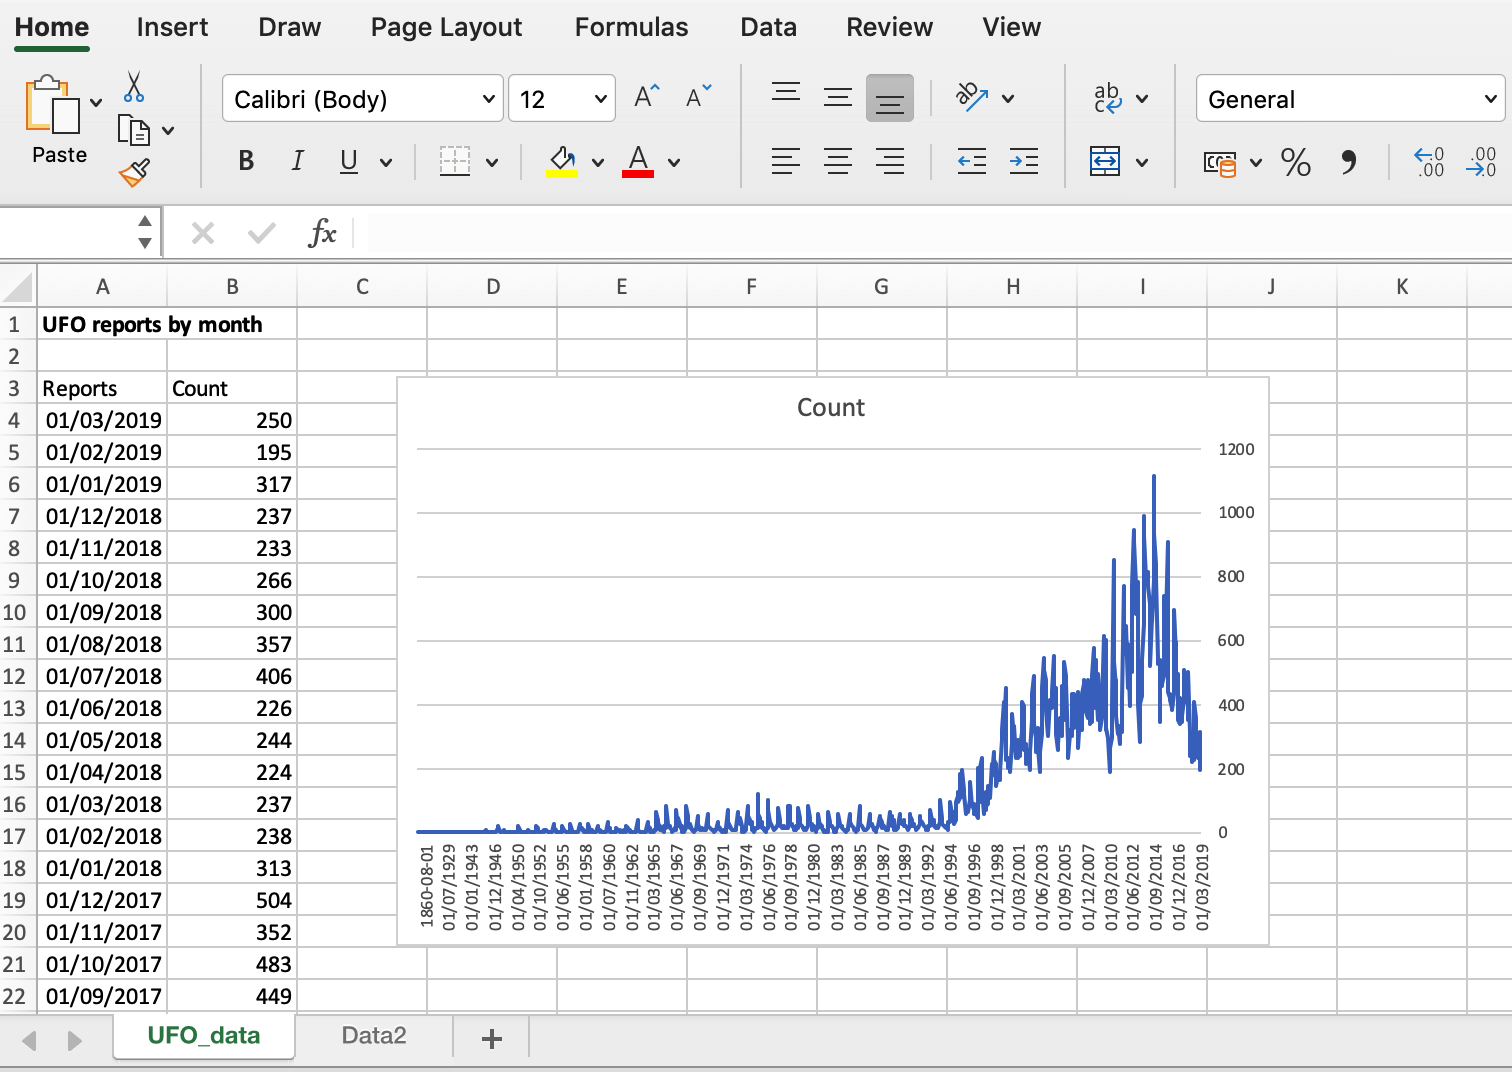
\includegraphics{Images/Excel_screenshot.png}
\caption{UFO spreadsheet}
\end{figure}

You can tell the \texttt{read\_excel()} function from the \texttt{readxl} package which sheet to read from and within that spreadsheet you can specify a range of cells to read from, so you can read the UFO data in like this:

\begin{Shaded}
\begin{Highlighting}[]
\NormalTok{UFO <-}\StringTok{ }\KeywordTok{read_excel}\NormalTok{(}\StringTok{"Data/UFO_data.xlsx"}\NormalTok{, }\DataTypeTok{sheet =} \StringTok{"UFO_data"}\NormalTok{, }\DataTypeTok{range =} \StringTok{"A3:B910"}\NormalTok{)}

\KeywordTok{str}\NormalTok{(UFO)}
\NormalTok{tibble [}\DecValTok{907}\NormalTok{ x }\DecValTok{2}\NormalTok{] (S3}\OperatorTok{:}\StringTok{ }\NormalTok{tbl_df}\OperatorTok{/}\NormalTok{tbl}\OperatorTok{/}\NormalTok{data.frame)}
 \OperatorTok{$}\StringTok{ }\NormalTok{Reports}\OperatorTok{:}\StringTok{ }\NormalTok{POSIXct[}\DecValTok{1}\OperatorTok{:}\DecValTok{907}\NormalTok{], format}\OperatorTok{:}\StringTok{ "2019-03-01"} \StringTok{"2019-02-01"}\NormalTok{ ...}
 \OperatorTok{$}\StringTok{ }\NormalTok{Count  }\OperatorTok{:}\StringTok{ }\NormalTok{num [}\DecValTok{1}\OperatorTok{:}\DecValTok{907}\NormalTok{] }\DecValTok{250} \DecValTok{195} \DecValTok{317} \DecValTok{237} \DecValTok{233} \DecValTok{266} \DecValTok{300} \DecValTok{357} \DecValTok{406} \DecValTok{226}\NormalTok{ ...}
\end{Highlighting}
\end{Shaded}

That worked nicely. Because I only included the data from 1900 onwards (you might rememebr that the dates for the years before those are in a different format) the ``Reports'' column has imported in the POSIXct class which is used to store dates and times. Nice!

A final point to make is that \texttt{readxl} is part of the \texttt{tidyverse} group of packages produced by Hadley Wickham and others at RStudio. One consequence of this is that the format of our imported data is not quite a normal data frame: rather it is something called a \emph{tibble}. You can see this if you just type the name of the object: if we had a normal data frame with 907 rows then typing its name would print the whole thing to the screen, or at least quite a lot of it depending on exactly how you have R set up. With a \emph{tibble} you get something different:

\begin{Shaded}
\begin{Highlighting}[]
\NormalTok{UFO}
\CommentTok{# A tibble: 907 x 2}
\NormalTok{   Reports             Count}
   \OperatorTok{<}\NormalTok{dttm}\OperatorTok{>}\StringTok{              }\ErrorTok{<}\NormalTok{dbl}\OperatorTok{>}
\StringTok{ }\DecValTok{1} \DecValTok{2019-03-01} \DecValTok{00}\OperatorTok{:}\DecValTok{00}\OperatorTok{:}\DecValTok{00}   \DecValTok{250}
 \DecValTok{2} \DecValTok{2019-02-01} \DecValTok{00}\OperatorTok{:}\DecValTok{00}\OperatorTok{:}\DecValTok{00}   \DecValTok{195}
 \DecValTok{3} \DecValTok{2019-01-01} \DecValTok{00}\OperatorTok{:}\DecValTok{00}\OperatorTok{:}\DecValTok{00}   \DecValTok{317}
 \DecValTok{4} \DecValTok{2018-12-01} \DecValTok{00}\OperatorTok{:}\DecValTok{00}\OperatorTok{:}\DecValTok{00}   \DecValTok{237}
 \DecValTok{5} \DecValTok{2018-11-01} \DecValTok{00}\OperatorTok{:}\DecValTok{00}\OperatorTok{:}\DecValTok{00}   \DecValTok{233}
 \DecValTok{6} \DecValTok{2018-10-01} \DecValTok{00}\OperatorTok{:}\DecValTok{00}\OperatorTok{:}\DecValTok{00}   \DecValTok{266}
 \DecValTok{7} \DecValTok{2018-09-01} \DecValTok{00}\OperatorTok{:}\DecValTok{00}\OperatorTok{:}\DecValTok{00}   \DecValTok{300}
 \DecValTok{8} \DecValTok{2018-08-01} \DecValTok{00}\OperatorTok{:}\DecValTok{00}\OperatorTok{:}\DecValTok{00}   \DecValTok{357}
 \DecValTok{9} \DecValTok{2018-07-01} \DecValTok{00}\OperatorTok{:}\DecValTok{00}\OperatorTok{:}\DecValTok{00}   \DecValTok{406}
\DecValTok{10} \DecValTok{2018-06-01} \DecValTok{00}\OperatorTok{:}\DecValTok{00}\OperatorTok{:}\DecValTok{00}   \DecValTok{226}
\CommentTok{# ... with 897 more rows}
\end{Highlighting}
\end{Shaded}

The difference is that you just get the top 10 rows and then an indication of how many more there are. There are some other differences between a tibble and a data frame but don't worry about them for the moment: you can treat it like a data frame for almost everything, and if you find it misbehaving you can always convert it to a data frame.

\begin{Shaded}
\begin{Highlighting}[]
\NormalTok{UFO <-}\StringTok{ }\KeywordTok{data.frame}\NormalTok{(UFO)}
\end{Highlighting}
\end{Shaded}

will do the trick.

\hypertarget{other-data-formats}{%
\section{Other data formats}\label{other-data-formats}}

Data often comes in other formats, and there are options for importing directly from these as well. The \texttt{foreign} package will read files from a wide variety of statistical software including Minitab, SPSS, STATA and SAS. The \texttt{Hmisc} package includes functions which will import data from SPSS, SAS and Stata as well, and \texttt{haven} will import from and export to SAS, SPSS and Stata formats. To import data from a Google Sheet have a look for the \texttt{googlesheets4} package which is \href{https://googlesheets4.tidyverse.org/}{currently in development}. It's still a bit tricky in my experience so be warned.

\hypertarget{importing-data-into-rstudio}{%
\section{Importing data into RStudio}\label{importing-data-into-rstudio}}

If you click on the `Environment' tab in RStudio you'll find that there is a clickable ``Import Dataset'' option which gives you options for importing from a variety of formats including Excel, SAS, SPSS, and Stata as well as from standard text files. What this does is open a window which gives you a clickable interface that then runs either the functions to import text from Base R or the import functions for other file formats from either the \texttt{readxl} or \texttt{haven}packages.

\hypertarget{to-attach-or-not-to-attach}{%
\section{To attach or not to attach?}\label{to-attach-or-not-to-attach}}

If you're doing a straightforward analysis and will only be using one data frame, you \emph{might} want to ``attach'' your data set.

\begin{Shaded}
\begin{Highlighting}[]
\KeywordTok{attach}\NormalTok{(mydata)}
\end{Highlighting}
\end{Shaded}

This is a bit arcane, but it can be quite handy. What it does is to tell R to put the data frame ``mydata'' into its ``search path''. This means that if you type the name of a variable in the data frame you don't need to tell R to look in the data frame to find it. For a data frame that is not attached you have to type the name of the data frame, a dollar sign and then the variable name: \texttt{mydata\$variablename}, but if you attach the data frame you can just type \texttt{variable\ name}.

To check whether a data frame is attached you can check the search path by using the \texttt{search()} function. This shows you the various things that R searches to look for objects or functions through when it receives an instruction.

\begin{Shaded}
\begin{Highlighting}[]
\KeywordTok{search}\NormalTok{()}
\NormalTok{ [}\DecValTok{1}\NormalTok{] }\StringTok{".GlobalEnv"}            \StringTok{"Counts"}                \StringTok{"package:xtable"}       
\NormalTok{ [}\DecValTok{4}\NormalTok{] }\StringTok{"package:ggplot2"}       \StringTok{"package:gplots"}        \StringTok{"package:lubridate"}    
\NormalTok{ [}\DecValTok{7}\NormalTok{] }\StringTok{"package:MASS"}          \StringTok{"package:scatterplot3d"} \StringTok{"package:RColorBrewer"} 
\NormalTok{[}\DecValTok{10}\NormalTok{] }\StringTok{"package:readxl"}        \StringTok{"package:stats"}         \StringTok{"package:graphics"}     
\NormalTok{[}\DecValTok{13}\NormalTok{] }\StringTok{"package:grDevices"}     \StringTok{"package:utils"}         \StringTok{"package:datasets"}     
\NormalTok{[}\DecValTok{16}\NormalTok{] }\StringTok{"package:methods"}       \StringTok{"Autoloads"}             \StringTok{"package:base"}         
\end{Highlighting}
\end{Shaded}

In this example I've attached the data frame ``Counts'' and you can see it as the second item in the search path. To remove something from the search path use \texttt{detach()}.

Opinions are mixed as to whether attaching your data frame is a good idea. If you're doing a big analysis and have several data frames, or if you're using a big data frame and you're subsetting parts of it to other objects for analysis then there's a lot of potential for errors, and the likelihood of analysing the wrong bit of data by mistake is reduced when you have to specify the data frame for analysis every time. Once upon a time I would have recommended that you attach your data frame for simple analyses only, but I've got a bit more hardcore over the years and I really think it's just bad practice that will lead to trouble if you do it.

\hypertarget{r-graphics-i-drawing-graphs-and-changing-plot-symbols-and-colours-using-the-base-graphics-system}{%
\chapter{R graphics I --- drawing graphs and changing plot symbols and colours using the base graphics system}\label{r-graphics-i-drawing-graphs-and-changing-plot-symbols-and-colours-using-the-base-graphics-system}}

When it comes to drawing graphs, using R gives you the same benefits and costs that you get when analysing data. Everything is done through a command-line interface that can be difficult to use and sometimes counterintuitive. Whereas with other software you get a nice GUI and can just point and click until you achieve what it is you're after, if you're drawing graphs in R you might have to do some research first to find out how to draw the graph you're after. That initial difficulty, however, is more than counterbalanced by the huge benefits of using R as your platform for data visualisation: R is almost infinitely flexible and can draw an extraordinary range of graphs, and you'll find that in many cases the default options are very good starting points; unlike those in a certain popular spreadsheet application, for example, they have been designed by people possessed of both brains and colour vision. Generating a script when you draw your graph means that you can easily return and edit your graph, and if you want to draw a similar graph with different data you can re-use your script with a few edits. Finally, you can use \emph{other peoples' scripts}. There are plenty of online resources with examples of graphs produced in R, and many of these have the code used to draw the graph associated with them. If you find an example of the sort of graph you want to make, you can use the code that's already there as the basis of your own script. Have a look at the \href{https://www.r-graph-gallery.com/}{R Graph Gallery}, a web resource set up for exactly this purpose, for an idea of the range of options available.

\hypertarget{base-graphics-versus-ggplot2-versus-lattice-versus-whaaat}{%
\section{Base graphics versus ggplot2 versus lattice versus whaaat???}\label{base-graphics-versus-ggplot2-versus-lattice-versus-whaaat}}

As a budding R user, your life has been made more complicated by the presence of a number of different options for creating graphics in R. Firstly, there is the graphics system which is built into R which is called \emph{base} graphics. Despite the implication from the name that it's a bit basic, this is a sophisticated and powerful system which can easily generate publication-quality graphs\ldots{} which is sometimes a surprise to the ggplot2 fanbois. There are then two main alternative systems, \emph{lattice} and \emph{ggplot2}, which work very differently to the base system. Of these, ggplot2 has become the most well-known, and many people are now using it exclusively. I don't think it's possible to be a fully functional R user nowadays without knowing at least the fundamentals of ggplot2, so in this chapter and the next we'll take an in-depth look at base graphics, and then we'll move on to some ggplot2 basics. You might not want to go through all of this so my advice is that if you're sure you want to stick to base graphics then read this chapter and the next. If you are probably going to go down the ggplot2 route, or you're not sure then you're probably best off reading this chapter, which introduces some important concepts that will be useful for ggplot2 as well as base graphics and then going on to the ggplot2 chapter.

\hypertarget{base-graphics-example-ufo-reports-again}{%
\section{Base graphics example: UFO reports again}\label{base-graphics-example-ufo-reports-again}}

We'll start off with looking at an example of how to produce a graph in R. In the previous chapter we looked at a script which drew a graph for you: the plot of UFO reports by month since 1900. Let's have another look at that script and go through the code. Here it is again.

\begin{Shaded}
\begin{Highlighting}[]
\CommentTok{# Script to read data on UFO reports and plot the data since 1900}
\CommentTok{# Audrey Bloggs 25th December 2022}

\CommentTok{# Load data from website}
\NormalTok{UFO <-}\StringTok{ }\KeywordTok{read.csv}\NormalTok{(}\StringTok{"http://www.introductoryr.co.uk/UFO_data.csv"}\NormalTok{,}
     \DataTypeTok{stringsAsFactors =} \OtherTok{FALSE}\NormalTok{)}

\CommentTok{# Convert 'Reports' variable to date}
\NormalTok{UFO}\OperatorTok{$}\NormalTok{Reports <-}\StringTok{ }\KeywordTok{as.Date}\NormalTok{(UFO}\OperatorTok{$}\NormalTok{Reports, }\DataTypeTok{format =} \StringTok{"%d/%m/%Y"}\NormalTok{)}

\CommentTok{# Trim off dates before 1900 which have a different format and convert to NA}
\NormalTok{UFO <-}\StringTok{ }\NormalTok{UFO[}\KeywordTok{which}\NormalTok{((}\OperatorTok{!}\KeywordTok{is.na}\NormalTok{(UFO}\OperatorTok{$}\NormalTok{Reports))), ]}

\CommentTok{# Check the data structure}
\KeywordTok{str}\NormalTok{(UFO)}

\CommentTok{# Plot the data}
\KeywordTok{plot}\NormalTok{(UFO}\OperatorTok{$}\NormalTok{Count }\OperatorTok{~}\StringTok{ }\NormalTok{UFO}\OperatorTok{$}\NormalTok{Reports,}
     \DataTypeTok{type =} \StringTok{"l"}\NormalTok{,}
     \DataTypeTok{col =} \StringTok{"steelblue"}\NormalTok{,}
     \DataTypeTok{xlab =} \StringTok{"Year"}\NormalTok{,}
     \DataTypeTok{ylab =} \StringTok{"Number of UFO reports by month"}\NormalTok{,}
     \DataTypeTok{main  =} \StringTok{"UFO reports by month since 1900"}\NormalTok{)}
\end{Highlighting}
\end{Shaded}

The first two thirds of the script are devoted to importing the data, cleaning it up and checking that everything's gone well, and then we have the \texttt{plot()} function call which actually draws the graph. \texttt{plot()} is a particularly flexible and powerful R function, and it can produce a wide range of different outputs depending on the nature of the data or R objects that we feed to it. Our complete function call looks like this.

\begin{Shaded}
\begin{Highlighting}[]
\KeywordTok{plot}\NormalTok{(UFO}\OperatorTok{$}\NormalTok{Count }\OperatorTok{~}\StringTok{ }\NormalTok{UFO}\OperatorTok{$}\NormalTok{Reports,}
     \DataTypeTok{type =} \StringTok{"l"}\NormalTok{,}
     \DataTypeTok{col =} \StringTok{"steelblue"}\NormalTok{,}
     \DataTypeTok{xlab =} \StringTok{"Year"}\NormalTok{,}
     \DataTypeTok{ylab =} \StringTok{"Number of UFO reports by month"}\NormalTok{,}
     \DataTypeTok{main  =} \StringTok{"UFO reports by month since 1900"}\NormalTok{)}
\end{Highlighting}
\end{Shaded}

Just like other functions in R we have a series of \emph{arguments} within the brackets, with each argument separated from the previous one by a comma. I've got each argument after the first on a separate line, which makes it easier to see what's happening in this piece of code. The first argument that we're giving to our \texttt{plot()} function tells it where to find the data to plot. In this case we're giving it two data variables, a numeric variable, \texttt{UFO\$Count} and a date variable \texttt{UFO\$Reports}, and they are separated by a tilde \texttt{\textasciitilde{}}. The tilde is an important symbol in R. This is the first time you've met it, but you'll see it a lot in defining formulas for statistical tests. You can think of it as meaning ``is explained by'' or as something which separates a \emph{dependent} variable from an \emph{independent} variable, or a \emph{response} variable from an \emph{explanatory} variable: if we think that one variable \emph{depends} on the value of the other then the former would be the dependent or response variable and the latter the independent or explanatory variable. In this case the number of UFO reports \emph{depends} on the year: there is clearly a big effect of year in determining the number of reports logged, but the year deosn't depend on the number of reports. No-one is going to say ``there have been 215 UFO reports, so we will call this year 2003''. Conventionally we put a dependent variable on the y-axis and an independent one on the x-axis, and this is what R will do.

If we just use the first argument, \texttt{UFO\$Count\ \textasciitilde{}\ UFO\$Reports} and none of the rest then R will go for the default option for a graph with continuous variables for both the x- and the y-axis, and draw a scatterplot with each data point represented by an open circle.

\begin{Shaded}
\begin{Highlighting}[]
\KeywordTok{plot}\NormalTok{(UFO}\OperatorTok{$}\NormalTok{Count }\OperatorTok{~}\StringTok{ }\NormalTok{UFO}\OperatorTok{$}\NormalTok{Reports)}
\end{Highlighting}
\end{Shaded}

\begin{figure}
\centering
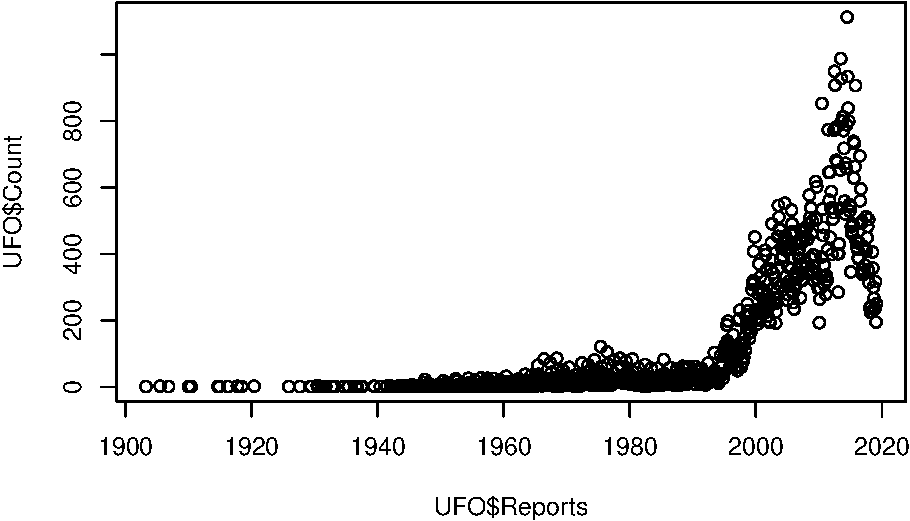
\includegraphics{3rd_Edition_files/figure-latex/graph1-1.pdf}
\caption{\label{fig:graph1}Scatterplot of UFO reports by year}
\end{figure}

That's not really what we're after and doesn't really show the important patterns in the data. We can tell R to draw a line connecting each data point instead of the scatterplot by adding the \texttt{type\ =\ \textquotesingle{}l\textquotesingle{}} argument:

\begin{Shaded}
\begin{Highlighting}[]
\KeywordTok{plot}\NormalTok{(UFO}\OperatorTok{$}\NormalTok{Count }\OperatorTok{~}\StringTok{ }\NormalTok{UFO}\OperatorTok{$}\NormalTok{Reports,}
     \DataTypeTok{type =} \StringTok{"l"}\NormalTok{)}
\end{Highlighting}
\end{Shaded}

\begin{figure}
\centering
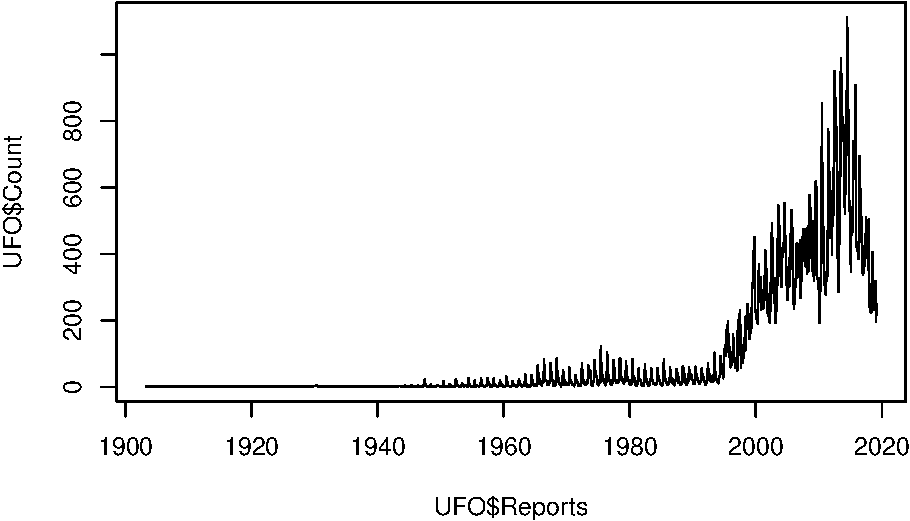
\includegraphics{3rd_Edition_files/figure-latex/graph2-1.pdf}
\caption{\label{fig:graph2}Line plot of UFO reports by year}
\end{figure}

which gives something much closer to what we're after. We can change the colour of the line using the \texttt{col\ =\ "steelblue"} argument, \texttt{xlab\ =\ "Year"} sets the axis label for the x-axis, \texttt{ylab\ =\ "Number\ of\ UFO\ reports\ by\ month"} does the same for the y-axis and finally \texttt{main\ \ =\ "UFO\ reports\ by\ month\ since\ 1900"} gives us a main title for the graph\ldots{}

\begin{Shaded}
\begin{Highlighting}[]
\KeywordTok{plot}\NormalTok{(UFO}\OperatorTok{$}\NormalTok{Count }\OperatorTok{~}\StringTok{ }\NormalTok{UFO}\OperatorTok{$}\NormalTok{Reports,}
     \DataTypeTok{type =} \StringTok{"l"}\NormalTok{,}
     \DataTypeTok{col =} \StringTok{"steelblue"}\NormalTok{,}
     \DataTypeTok{xlab =} \StringTok{"Year"}\NormalTok{,}
     \DataTypeTok{ylab =} \StringTok{"Number of UFO reports by month"}\NormalTok{,}
     \DataTypeTok{main  =} \StringTok{"UFO reports by month since 1900"}\NormalTok{)}
\end{Highlighting}
\end{Shaded}

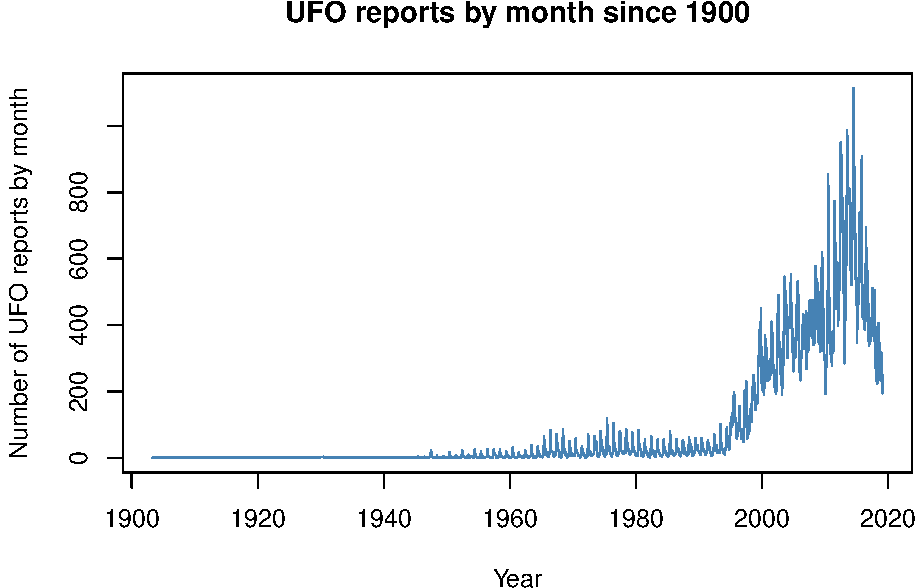
\includegraphics{3rd_Edition_files/figure-latex/unnamed-chunk-215-1.pdf}

\ldots{} and with remarkably little fuss we have a nice, publication quality graph displaying our data. This example shows us the basics of producing graphs in R: the \texttt{plot()} function produces a particular kind of graph depending on the data that you feed it, but you can then modify the look of the graph and change things like the axis labels by using further arguments to your \texttt{plot()} function call. It's worth pointing out here that these arguments are often called graphical \emph{parameters} when we're referring to arguments that change the appearance of a graph, but they work in the same way as arguments for other types of function. We'll talk a little more about graphical parameters later on in the chapter.

\hypertarget{scatterplots}{%
\section{Scatterplots}\label{scatterplots}}

Let's look at scatterplots in rather more detail. We'll draw a scatterplot and then specify the shape and colour of the datapoints according to some classification, then finally we'll add some fitted lines to our data. The dataset we'll be using is from a paper published in the Journal of Evolutionary Biology by John Fitzpatrick and coauthors\footnote{Fitzpatrick, J.L., Almbro, M., Gonzalez-Voyer, A., Hamada, S., Pennington, C., Scanlan, J. \& Kolm, N. (2012) Sexual selection uncouples the evolution of brain and body size in pinnipeds. Journal of evolutionary biology, 25, 1321--1330.} on the subject of how brain size in pinnipeds (seals, walruses and sea lions) relates to their mating system. The fundamental question they were addressing is whether brain size varies between seals where the males defend groups of females (``harems''), and species where males pair up with single females.

The dataset is online and you can load it straight into R from the web by running this line of code.

\begin{Shaded}
\begin{Highlighting}[]
\NormalTok{pinniped <-}\StringTok{ }\KeywordTok{read.csv}\NormalTok{(}\StringTok{"http://www.introductoryr.co.uk/Pinniped_brains.csv"}\NormalTok{, }\DataTypeTok{stringsAsFactors =} \OtherTok{FALSE}\NormalTok{)}
\end{Highlighting}
\end{Shaded}

As always, we want to know whether our dataset has imported properly so we check using the \texttt{str()} function.

\begin{Shaded}
\begin{Highlighting}[]
\KeywordTok{str}\NormalTok{(pinniped)}
\StringTok{'data.frame'}\OperatorTok{:}\StringTok{   }\DecValTok{33}\NormalTok{ obs. of  }\DecValTok{11}\NormalTok{ variables}\OperatorTok{:}
\StringTok{ }\ErrorTok{$}\StringTok{ }\NormalTok{Species        }\OperatorTok{:}\StringTok{ }\NormalTok{chr  }\StringTok{"Monachus schauinslandi"} \StringTok{"Monachus monachus"} \StringTok{"Mirounga angustirostris"} \StringTok{"Mirounga leonina"}\NormalTok{ ...}
 \OperatorTok{$}\StringTok{ }\NormalTok{Male_brain     }\OperatorTok{:}\StringTok{ }\NormalTok{num  }\DecValTok{370} \DecValTok{480} \DecValTok{700} \DecValTok{1431} \DecValTok{535}\NormalTok{ ...}
 \OperatorTok{$}\StringTok{ }\NormalTok{Female_brain   }\OperatorTok{:}\StringTok{ }\NormalTok{num  }\OtherTok{NA} \DecValTok{480} \DecValTok{640} \DecValTok{899} \DecValTok{638}\NormalTok{ ...}
 \OperatorTok{$}\StringTok{ }\NormalTok{Male_mass      }\OperatorTok{:}\StringTok{ }\NormalTok{num  }\DecValTok{173} \DecValTok{260} \DecValTok{2275} \DecValTok{3510} \DecValTok{450}\NormalTok{ ...}
 \OperatorTok{$}\StringTok{ }\NormalTok{Female_mass    }\OperatorTok{:}\StringTok{ }\NormalTok{num  }\DecValTok{272} \DecValTok{275} \DecValTok{488} \DecValTok{566} \DecValTok{447}\NormalTok{ ...}
 \OperatorTok{$}\StringTok{ }\NormalTok{Harem          }\OperatorTok{:}\StringTok{ }\NormalTok{num  }\DecValTok{1} \DecValTok{1} \DecValTok{13} \DecValTok{48} \DecValTok{3} \DecValTok{1} \DecValTok{1} \DecValTok{1} \DecValTok{1} \DecValTok{1}\NormalTok{ ...}
 \OperatorTok{$}\StringTok{ }\NormalTok{Small_intestine}\OperatorTok{:}\StringTok{ }\NormalTok{int  }\DecValTok{1030} \DecValTok{870} \DecValTok{3820} \DecValTok{12100} \DecValTok{2700} \DecValTok{790} \DecValTok{2530} \DecValTok{2190} \DecValTok{2520} \DecValTok{2164}\NormalTok{ ...}
 \OperatorTok{$}\StringTok{ }\NormalTok{Gestation      }\OperatorTok{:}\StringTok{ }\NormalTok{int  }\DecValTok{330} \DecValTok{330} \DecValTok{230} \DecValTok{225} \DecValTok{263} \DecValTok{248} \DecValTok{255} \DecValTok{276} \DecValTok{234} \DecValTok{270}\NormalTok{ ...}
 \OperatorTok{$}\StringTok{ }\NormalTok{Lifespan       }\OperatorTok{:}\StringTok{ }\NormalTok{num  }\DecValTok{360} \DecValTok{284} \DecValTok{244} \DecValTok{276} \DecValTok{300}\NormalTok{ ...}
 \OperatorTok{$}\StringTok{ }\NormalTok{Lactation      }\OperatorTok{:}\StringTok{ }\NormalTok{int  }\DecValTok{38} \DecValTok{42} \DecValTok{26} \DecValTok{23} \DecValTok{50} \DecValTok{30} \DecValTok{17} \DecValTok{29} \DecValTok{4} \DecValTok{24}\NormalTok{ ...}
 \OperatorTok{$}\StringTok{ }\NormalTok{Dive_duration  }\OperatorTok{:}\StringTok{ }\NormalTok{num  }\DecValTok{12} \OtherTok{NA} \DecValTok{62} \DecValTok{120} \DecValTok{82} \FloatTok{9.8} \FloatTok{10.8} \OtherTok{NA} \DecValTok{52} \DecValTok{25}\NormalTok{ ...}
\end{Highlighting}
\end{Shaded}

All good: we have quite a few variables including a character vector of species names, male and female brain mass (g), male and female body mass (Kg) and the average harem size, where 1 indicates each male is only mating with a single female at a time and values greater than 1 tell us that males, if they are able, will guard females in groups.

Let's plot male brain mass against body mass to start with.

\begin{Shaded}
\begin{Highlighting}[]
\KeywordTok{plot}\NormalTok{(pinniped}\OperatorTok{$}\NormalTok{Male_brain}\OperatorTok{~}\NormalTok{pinniped}\OperatorTok{$}\NormalTok{Male_mass)}
\end{Highlighting}
\end{Shaded}

\begin{figure}
\centering
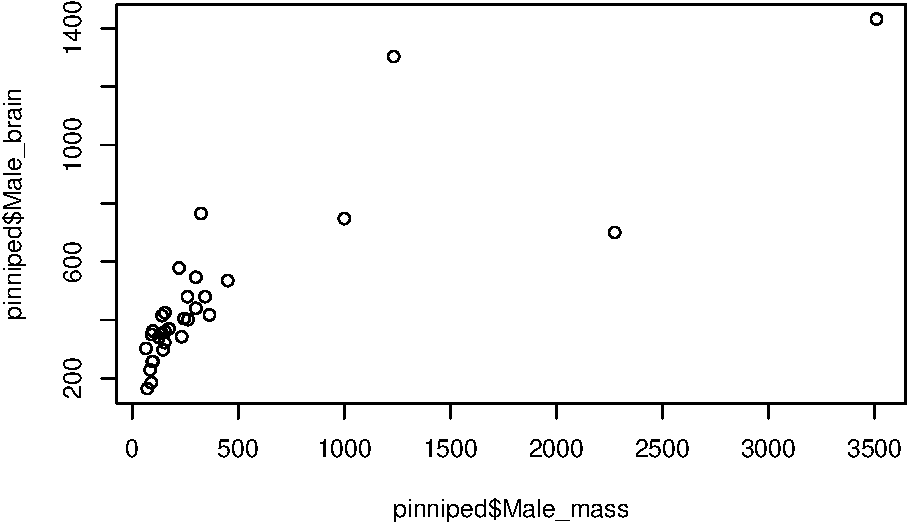
\includegraphics{3rd_Edition_files/figure-latex/graph3-1.pdf}
\caption{\label{fig:graph3}Brain mass versus body mass for 33 species of male pinniped}
\end{figure}

This plot is showing us that there is some sort of relationship between brain mass and body mass, but it is difficult to tell much from it because both the brain mass and body mass data are squished down into the bottom left corner. This is because both of these variables are \emph{positively skewed}: there are lots of seals and their relatives with body mass between about 50 and about 500Kg, but then there are a few which are much heavier up to \emph{Mirounga leonina}, the Southern Elephant Seal, which is an absolute chonker with males weighing in at about 3.5 metric tonnes. We need to do something to spread the data out more evenly, and usually when dealing with this sort of \emph{positively skewed} data we'd plot the log transformed data rather than the raw data. There are two easy ways to do this in R: you can generate new variables which are the logged values that you want to plot, or you can use an argument within the \texttt{plot()} function call to tell it to plot the data on a log scale.

Here is the first option.

\begin{Shaded}
\begin{Highlighting}[]
\CommentTok{#Generate new variables with the log transformed data}
\NormalTok{log_Male_brain <-}\StringTok{ }\KeywordTok{log}\NormalTok{(pinniped}\OperatorTok{$}\NormalTok{Male_brain)}
\NormalTok{log_Male_mass <-}\StringTok{ }\KeywordTok{log}\NormalTok{(pinniped}\OperatorTok{$}\NormalTok{Male_mass)}

\CommentTok{#plot our new variables}
\KeywordTok{plot}\NormalTok{(log_Male_brain}\OperatorTok{~}\NormalTok{log_Male_mass)}
\end{Highlighting}
\end{Shaded}

\begin{figure}
\centering
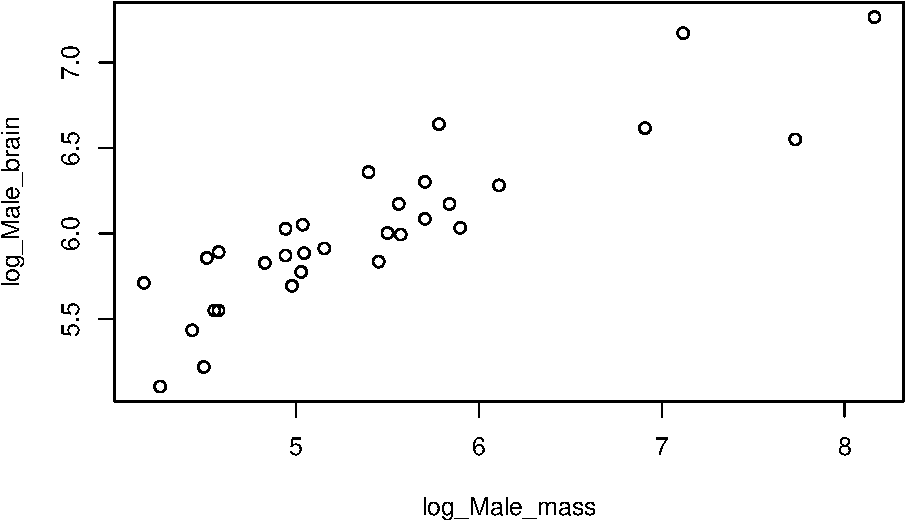
\includegraphics{3rd_Edition_files/figure-latex/graph4-1.pdf}
\caption{\label{fig:graph4}Log brain mass versus log body mass for 33 species of male pinniped}
\end{figure}

You can see that log transforming these data gives us a nice looking plot with the data spread out so that we can see any patterns that might be there. How about the other alternative?

\begin{Shaded}
\begin{Highlighting}[]
\KeywordTok{plot}\NormalTok{(pinniped}\OperatorTok{$}\NormalTok{Male_brain }\OperatorTok{~}\StringTok{ }\NormalTok{pinniped}\OperatorTok{$}\NormalTok{Male_mass,}
     \DataTypeTok{log  =} \StringTok{"xy"}\NormalTok{)}
\end{Highlighting}
\end{Shaded}

\begin{figure}
\centering
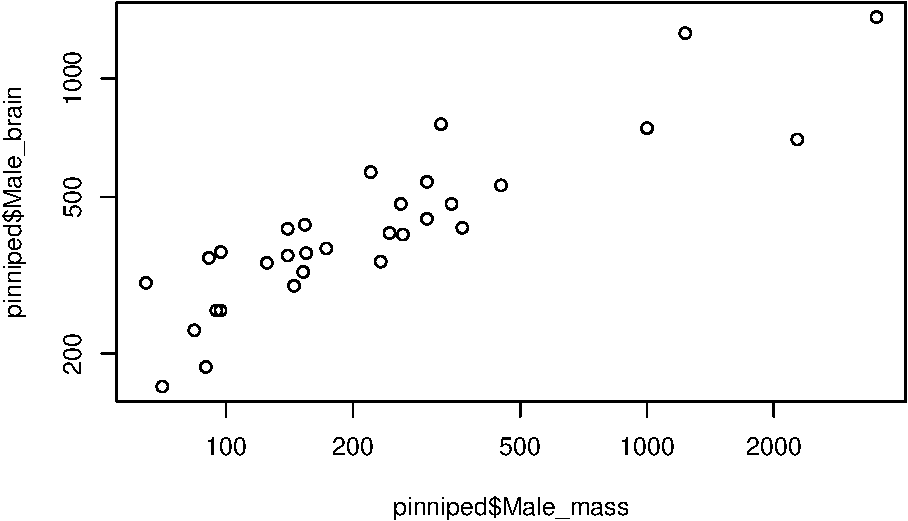
\includegraphics{3rd_Edition_files/figure-latex/graph5-1.pdf}
\caption{\label{fig:graph5}Brain mass versus body mass for 33 species of male pinniped, plotted on log scaled axes}
\end{figure}

The positioning of the points is exactly the same, but the numbers on the axes are different. What's happened here is that instead of log-transforming the data we've plotted the untransformed data on axes that are on log scales ----- you can see this by looking at the numbers on the x-axis in particular, where the distance from 100 to 200 is about the same as the distance from 1000 to 2000. If you only wanted the y-axis plotted on a log scale you could use \texttt{log\ =\ "y"} and if you only wanted the x-axis on a log scale then \texttt{log\ =\ "x"} would do.

Which of these options for plotting logged data you use is up to you and the best option will depend on the context. I generally prefer the latter, since you retain the original units for your axes which makes it easier to understand what each data point represents.

Talking of units, the axis labels on our plot are not especially informative, so let's fix that by telling the \texttt{plot()} function what we want our axis labels to be. We can do that using the \texttt{xlab\ =} and \texttt{ylab\ =} arguments.

\begin{Shaded}
\begin{Highlighting}[]
\KeywordTok{plot}\NormalTok{(pinniped}\OperatorTok{$}\NormalTok{Male_brain }\OperatorTok{~}\StringTok{ }\NormalTok{pinniped}\OperatorTok{$}\NormalTok{Male_mass,}
     \DataTypeTok{log  =} \StringTok{"xy"}\NormalTok{,}
     \DataTypeTok{xlab =} \StringTok{"Body mass (Kg)"}\NormalTok{,}
     \DataTypeTok{ylab =} \StringTok{"Brain mass (g)"}\NormalTok{)}
\end{Highlighting}
\end{Shaded}

\begin{figure}
\centering
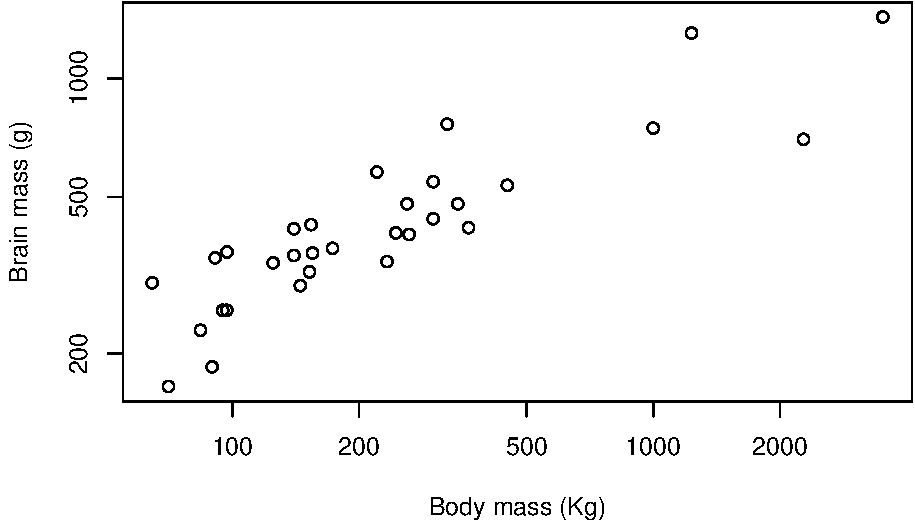
\includegraphics{3rd_Edition_files/figure-latex/graph6-1.pdf}
\caption{\label{fig:graph6}Brain mass versus body mass for 33 species of male pinniped plotted on log scaled axes}
\end{figure}

Good. This is now looking like a graph that we might start to think about publishing. You can see how the default options for things like axis limits and plot symbols are clean and well chosen in base R graphics. We've not finished though: we want to change our graph so that the viewer can differentiate between species with ``harem'' mating systems and other species.

The Harem variable in our data set tells us the average size of the group of females that a male will defend for each species, so if Harem = 1 then we can classify a species as a non-harem one, and if Harem \textgreater{} 1 then we can classify a species as one with a harem mating system. We can then use subscripting to allocate a specific colour or plot symbol to the data points for harem or non-harem species.

\hypertarget{plot-symbols}{%
\section{Plot symbols}\label{plot-symbols}}

We can get R to draw different plot symbols by using the \texttt{pch\ =} graphical parameter. R has a set of built in symbols that are represented by the numbers 1 to 25. Here they are:

Click here to see the code

\begin{Shaded}
\begin{Highlighting}[]
\CommentTok{# Set up variables}
\NormalTok{X1 <-}\StringTok{ }\KeywordTok{rep}\NormalTok{(}\DecValTok{1}\OperatorTok{:}\DecValTok{5}\NormalTok{, }\DecValTok{5}\NormalTok{)}
\NormalTok{Y1 <-}\StringTok{ }\KeywordTok{rep}\NormalTok{(}\DecValTok{5}\OperatorTok{:}\DecValTok{1}\NormalTok{, }\DataTypeTok{each =} \DecValTok{5}\NormalTok{)}
\NormalTok{sym <-}\StringTok{ }\DecValTok{1}\OperatorTok{:}\DecValTok{25}

\CommentTok{# Plot the graph}
\KeywordTok{plot}\NormalTok{(}
\NormalTok{  X1,}
\NormalTok{  Y1,}
  \DataTypeTok{pch =}\NormalTok{ sym,}
  \DataTypeTok{cex =} \FloatTok{1.2}\NormalTok{,}
  \DataTypeTok{xlab =} \StringTok{""}\NormalTok{,}
  \DataTypeTok{ylab =} \StringTok{""}\NormalTok{,}
  \DataTypeTok{xaxt =} \StringTok{"n"}\NormalTok{,}
  \DataTypeTok{yaxt =} \StringTok{"n"}\NormalTok{,}
  \DataTypeTok{xlim =} \KeywordTok{c}\NormalTok{(}\FloatTok{0.3}\NormalTok{, }\FloatTok{5.7}\NormalTok{),}
  \DataTypeTok{ylim =} \KeywordTok{c}\NormalTok{(}\FloatTok{0.3}\NormalTok{, }\FloatTok{5.7}\NormalTok{)}
\NormalTok{)}

\CommentTok{# Add text}
\KeywordTok{text}\NormalTok{(}\DataTypeTok{x =}\NormalTok{ X1 }\OperatorTok{-}\StringTok{ }\FloatTok{0.3}\NormalTok{, }\DataTypeTok{y =}\NormalTok{ Y1, }\DataTypeTok{labels =}\NormalTok{ sym)}
\end{Highlighting}
\end{Shaded}

\begin{figure}
\centering
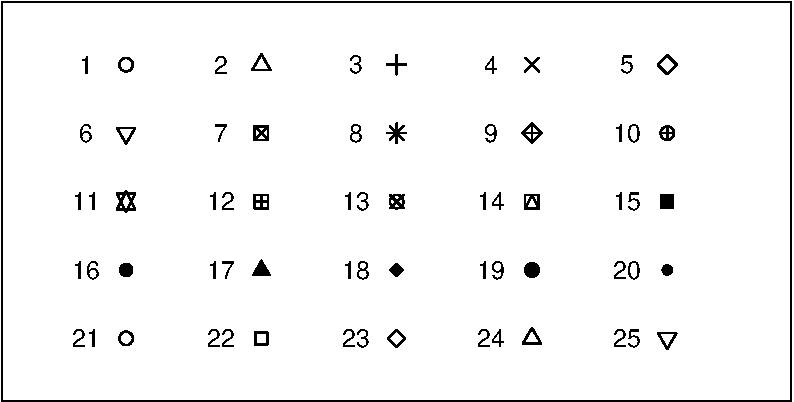
\includegraphics{3rd_Edition_files/figure-latex/graph7-1.pdf}
\caption{\label{fig:graph7}Plot symbols used in R}
\end{figure}

So if we'd like to plot our data with filled circles instead of open ones, we can set \texttt{pch\ =\ 16} as one of our graphical arguments, like this.

\begin{Shaded}
\begin{Highlighting}[]
\KeywordTok{plot}\NormalTok{(pinniped}\OperatorTok{$}\NormalTok{Male_brain }\OperatorTok{~}\StringTok{ }\NormalTok{pinniped}\OperatorTok{$}\NormalTok{Male_mass,}
     \DataTypeTok{log  =} \StringTok{"xy"}\NormalTok{,}
     \DataTypeTok{xlab =} \StringTok{"Body mass (Kg)"}\NormalTok{,}
     \DataTypeTok{ylab =} \StringTok{"Brain mass (g)"}\NormalTok{, }
     \DataTypeTok{pch =} \DecValTok{16}\NormalTok{)}
\end{Highlighting}
\end{Shaded}

\begin{figure}
\centering
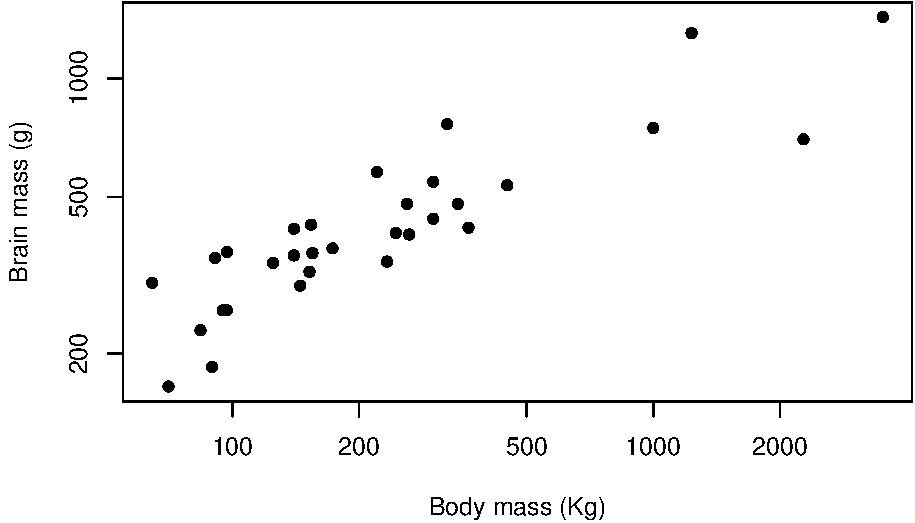
\includegraphics{3rd_Edition_files/figure-latex/graph8-1.pdf}
\caption{\label{fig:graph8}Brain mass versus body mass for 33 species of male pinniped plotted on log scaled axes using closed circles as plot symbols}
\end{figure}

\hypertarget{colours}{%
\section{Colours}\label{colours}}

The colour or colours that your plot symbols are drawn with (or the colours of the boxes in a boxplot, or the bars in a histogram or bar plot) can be set in R by using the \emph{col} parameter, and other parameters such as \emph{bg}, \emph{col.axis}, \emph{col.lab} set the colours for other parts of the plot: these examples will allow you to change the background colour and the colours of the axes and the axis labels respectively. For a full list of these take a look at \texttt{?par} which will bring up a description of all of the graphical parameters. The actual colours to be used can be named in a confusing variety of different ways, but for the beginner the easiest thing to do is simply to use the name: ``red'', ``blue'', ``green'' or ``lightblue'' or ``darkgreen''. In fact, R has a rather surprising number of named colours that you can use, and an even more surprising range of names, from ``aliceblue'' through ``darkgoldenrod2'', ``hotpink1'', ``lemonchiffon3'' to ``tomato4''. The function \texttt{colours()}, or \texttt{colors()} if you prefer the American spelling will produce a list of all 657 named colours in R. Appendix 1 has a series of charts showing each colour with its name.

If you're familiar with how colours are described in computers then you can use the RGB hexadecimal code for the colour: this begins with a hash symbol and then has two numbers for the red channel (computers think in hexadecimal to each one is 0-9 and the A-F), two for the green and two for the blue, so \#0000FF is blue, \#FF0000 is red, \#000000 is black and \#FFFFFF is white. We'll talk about using these hex codes a little later when we discuss using \emph{alpha channels} to make elements of your graph semi-transparent.

If we wanted to change the colours of our plot symbols from the default black option we just need to add another argument specifying the exact colour we want. If we wanted \emph{aquamarine4} as our plot colour then our code would look like this.

\begin{Shaded}
\begin{Highlighting}[]
\KeywordTok{plot}\NormalTok{(pinniped}\OperatorTok{$}\NormalTok{Male_brain }\OperatorTok{~}\StringTok{ }\NormalTok{pinniped}\OperatorTok{$}\NormalTok{Male_mass,}
     \DataTypeTok{log  =} \StringTok{"xy"}\NormalTok{,}
     \DataTypeTok{xlab =} \StringTok{"Body mass (Kg)"}\NormalTok{,}
     \DataTypeTok{ylab =} \StringTok{"Brain mass (g)"}\NormalTok{, }
     \DataTypeTok{pch =} \DecValTok{16}\NormalTok{,}
     \DataTypeTok{col =} \StringTok{"aquamarine4"}\NormalTok{)}
\end{Highlighting}
\end{Shaded}

\begin{figure}
\centering
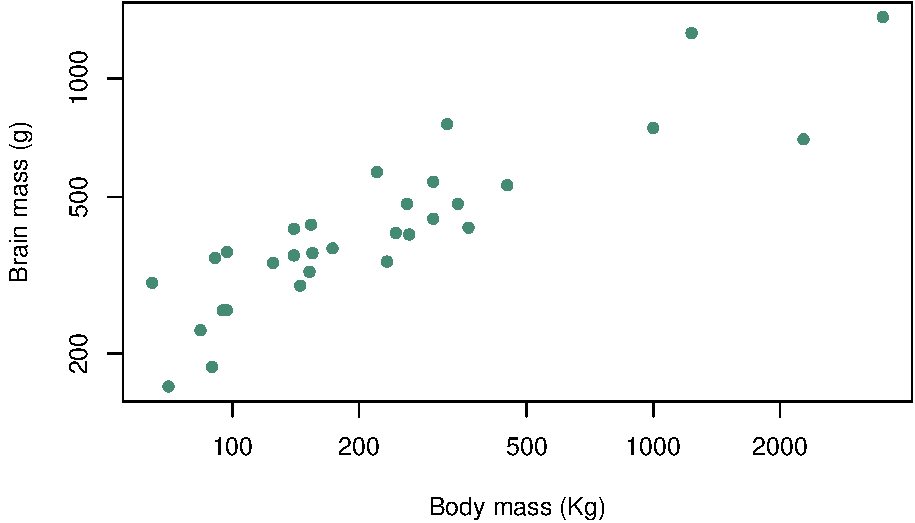
\includegraphics{3rd_Edition_files/figure-latex/graph9-1.pdf}
\caption{\label{fig:graph9}Brain mass versus body mass for 33 species of male pinniped plotted on log scaled axes with both plot symbol and colour specified}
\end{figure}

\hypertarget{plotting-multiple-symbols-or-colours}{%
\section{Plotting multiple symbols or colours}\label{plotting-multiple-symbols-or-colours}}

One of the most important uses of colour or plot symbols is to distinguish between different classes of data, and this is something that we can do in R: if we have a variable which classifies our data into groups, then we can use that to tell R which colours or symbols to use. Using our data on pinnipeds, we can divide our species into harem breeders, where males defend groups of more than one female during the mating season, and non-harem breeders where each male is only associated with a single female. The variable \texttt{Harem} gives us the number of females that a male might be associated with and we can use this to set up a new factor called \texttt{Mating\_system} which has two levels, \texttt{Harem} for males who will seek to defend more than one female and \texttt{Non\ harem} for males who only associate with a single female at a time.

\begin{Shaded}
\begin{Highlighting}[]
\NormalTok{Mating_system <-}\StringTok{ }\KeywordTok{factor}\NormalTok{(}\KeywordTok{ifelse}\NormalTok{(pinniped}\OperatorTok{$}\NormalTok{Harem }\OperatorTok{==}\StringTok{ }\DecValTok{1}\NormalTok{, }\StringTok{"Non harem"}\NormalTok{, }\StringTok{"Harem"}\NormalTok{))}
\end{Highlighting}
\end{Shaded}

Here we've used the \texttt{ifelse()} function which takes a logical statement, in this case whether the value of \texttt{Harem} is equal to one, and returns one value, in this case \texttt{"Non\ harem"}, if the logical statement is true and a second value (\texttt{"Harem"}) if the statement is false. Now we can plot our data and indicate to the viewer which mating system is associated with each data point. Firstly we'll do this with colours, and then with different plot symbols.

To indicate how our points are classified we need a vector of colours for R to use in our plot. This example has only two but if you have more groups you just need more colours in your vector.

\begin{Shaded}
\begin{Highlighting}[]
\NormalTok{colours <-}\StringTok{ }\KeywordTok{c}\NormalTok{(}\StringTok{"aquamarine4"}\NormalTok{, }\StringTok{"chocolate2"}\NormalTok{)}
\end{Highlighting}
\end{Shaded}

Now we have a vector of colours and a factor which classifies our data. How do we use these to generate a plot with each data point colour coded by the factor levels? The answer lies in some clever use of subscripts. \texttt{colours} is a character vector and we can retrieve the first or second value by using a subscript:

\begin{Shaded}
\begin{Highlighting}[]
\NormalTok{colours[}\DecValTok{2}\NormalTok{]}
\NormalTok{[}\DecValTok{1}\NormalTok{] }\StringTok{"chocolate2"}
\end{Highlighting}
\end{Shaded}

returns the second value in the vector. If we have a second vector of numbers which correspond to the useable subscripts for our \texttt{colours} vector then we can use this to generate a new vector of colour names:

\begin{Shaded}
\begin{Highlighting}[]
\NormalTok{example <-}\StringTok{ }\KeywordTok{c}\NormalTok{(}\DecValTok{1}\NormalTok{,}\DecValTok{1}\NormalTok{,}\DecValTok{2}\NormalTok{,}\DecValTok{1}\NormalTok{,}\DecValTok{2}\NormalTok{,}\DecValTok{2}\NormalTok{,}\DecValTok{1}\NormalTok{)}
\NormalTok{colours[example]}
\NormalTok{[}\DecValTok{1}\NormalTok{] }\StringTok{"aquamarine4"} \StringTok{"aquamarine4"} \StringTok{"chocolate2"}  \StringTok{"aquamarine4"} \StringTok{"chocolate2"} 
\NormalTok{[}\DecValTok{6}\NormalTok{] }\StringTok{"chocolate2"}  \StringTok{"aquamarine4"}
\end{Highlighting}
\end{Shaded}

which returns a vector with seven colour names, each corresponding to the relevant value in our \texttt{example} vector. Now let's go back to our \texttt{Mating\_system} factor. This has two levels, \texttt{Harem} and \texttt{Non\ harem} and these levels will be coded by R as \texttt{1} for \texttt{Harem}, which coes first alphabetically, and \texttt{2} for \texttt{Non\ harem} which comes second. If, therefore, we use \texttt{Mating\_system} as a subscript for \texttt{colours} it should return \texttt{"aquamarine4"} for each value of \texttt{Non\ harem} in \texttt{Mating\_system} and \texttt{"chocolate2"} for each value of \texttt{Harem}. Let's try that out.

\begin{Shaded}
\begin{Highlighting}[]
\NormalTok{colours[Mating_system]}
\NormalTok{ [}\DecValTok{1}\NormalTok{] }\StringTok{"chocolate2"}  \StringTok{"chocolate2"}  \StringTok{"aquamarine4"} \StringTok{"aquamarine4"} \StringTok{"aquamarine4"}
\NormalTok{ [}\DecValTok{6}\NormalTok{] }\StringTok{"chocolate2"}  \StringTok{"chocolate2"}  \StringTok{"chocolate2"}  \StringTok{"chocolate2"}  \StringTok{"chocolate2"} 
\NormalTok{[}\DecValTok{11}\NormalTok{] }\StringTok{"aquamarine4"} \StringTok{"chocolate2"}  \StringTok{"chocolate2"}  \StringTok{"chocolate2"}  \StringTok{"chocolate2"} 
\NormalTok{[}\DecValTok{16}\NormalTok{] }\StringTok{"chocolate2"}  \StringTok{"chocolate2"}  \StringTok{"chocolate2"}  \StringTok{"aquamarine4"} \StringTok{"aquamarine4"}
\NormalTok{[}\DecValTok{21}\NormalTok{] }\StringTok{"aquamarine4"} \StringTok{"aquamarine4"} \StringTok{"aquamarine4"} \StringTok{"aquamarine4"} \StringTok{"aquamarine4"}
\NormalTok{[}\DecValTok{26}\NormalTok{] }\StringTok{"aquamarine4"} \StringTok{"aquamarine4"} \StringTok{"aquamarine4"} \StringTok{"aquamarine4"} \StringTok{"aquamarine4"}
\NormalTok{[}\DecValTok{31}\NormalTok{] }\StringTok{"aquamarine4"} \StringTok{"aquamarine4"} \StringTok{"aquamarine4"}
\end{Highlighting}
\end{Shaded}

\emph{Et voilà!} we can generate a vector of colours which we can include in our \texttt{plot()} function call with only a very brief piece of code.

\begin{Shaded}
\begin{Highlighting}[]
\KeywordTok{plot}\NormalTok{(pinniped}\OperatorTok{$}\NormalTok{Male_brain }\OperatorTok{~}\StringTok{ }\NormalTok{pinniped}\OperatorTok{$}\NormalTok{Male_mass,}
     \DataTypeTok{log  =} \StringTok{"xy"}\NormalTok{,}
     \DataTypeTok{xlab =} \StringTok{"Body mass (Kg)"}\NormalTok{,}
     \DataTypeTok{ylab =} \StringTok{"Brain mass (g)"}\NormalTok{, }
     \DataTypeTok{pch =} \DecValTok{16}\NormalTok{,}
     \DataTypeTok{col =}\NormalTok{ colours[Mating_system])}
\end{Highlighting}
\end{Shaded}

\begin{figure}
\centering
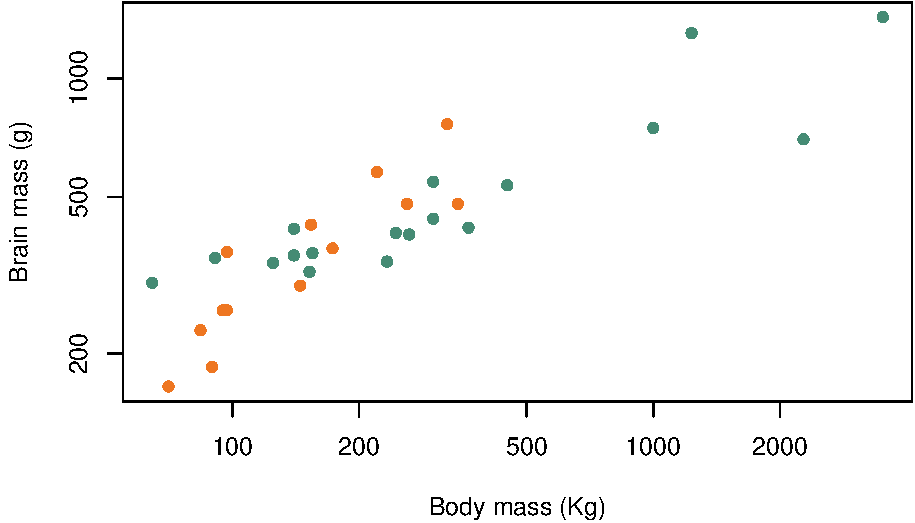
\includegraphics{3rd_Edition_files/figure-latex/graph10-1.pdf}
\caption{\label{fig:graph10}Brain mass versus body mass for 33 species of male pinniped plotted on log scaled axes, orange symbols indicate non-harem breeders and green indicate harem breeders}
\end{figure}

There we are. Now, if I were given chocolate that colour to eat I'd be rather dubious, but aside from that we've achieved our goal.

We can vary the plot symbol using the exact same logic. If we wanted to indicate mating system by using a filled circle (plot symbol 16) for \texttt{Harem} and a filled triangle (plot symbol 17) for \texttt{Non\ harem} we need to set up a vector containing these two numbers:

\begin{Shaded}
\begin{Highlighting}[]
\NormalTok{symbols <-}\StringTok{ }\KeywordTok{c}\NormalTok{(}\DecValTok{16}\NormalTok{,}\DecValTok{17}\NormalTok{)}
\end{Highlighting}
\end{Shaded}

and then we can use this in our \texttt{plot()} function call with a subscript in the same way that we did for colours.

\begin{Shaded}
\begin{Highlighting}[]
\KeywordTok{plot}\NormalTok{(pinniped}\OperatorTok{$}\NormalTok{Male_brain }\OperatorTok{~}\StringTok{ }\NormalTok{pinniped}\OperatorTok{$}\NormalTok{Male_mass,}
     \DataTypeTok{log  =} \StringTok{"xy"}\NormalTok{,}
     \DataTypeTok{xlab =} \StringTok{"Body mass (Kg)"}\NormalTok{,}
     \DataTypeTok{ylab =} \StringTok{"Brain mass (g)"}\NormalTok{, }
     \DataTypeTok{pch =}\NormalTok{ symbols[Mating_system])}
\end{Highlighting}
\end{Shaded}

\begin{figure}
\centering
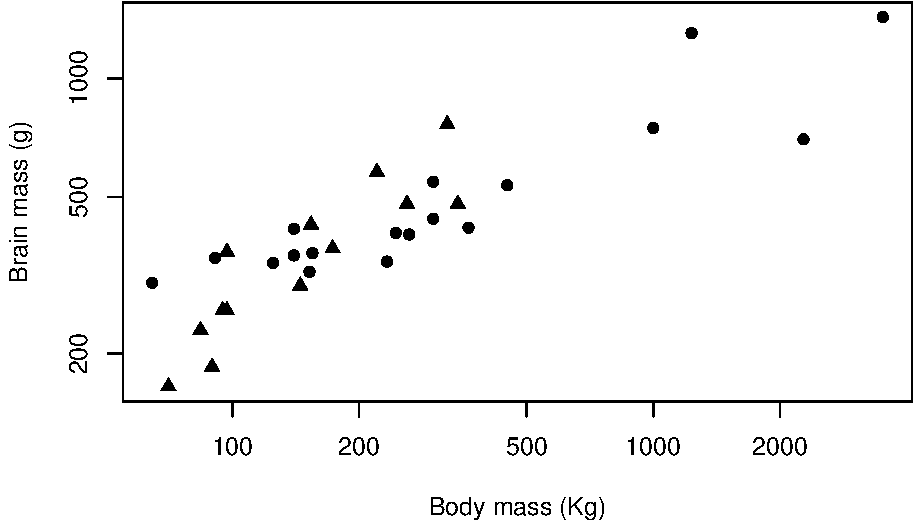
\includegraphics{3rd_Edition_files/figure-latex/unnamed-chunk-225-1.pdf}
\caption{\label{fig:unnamed-chunk-225}Brain mass versus body mass for 33 species of male pinniped plotted on log scaled axes, triangles indicate non-harem breeders and circles indicate harem breeders}
\end{figure}

\hypertarget{colour-palettes-in-r}{%
\section{Colour palettes in R}\label{colour-palettes-in-r}}

You don't have to choose your own colours for your plots. R has a number of built-in selections of colours which are known as ``palettes''. There is a default palette which is a vector of 8 different colours which can be found using the \texttt{palette()} function.

\begin{Shaded}
\begin{Highlighting}[]
\KeywordTok{palette}\NormalTok{()}
\NormalTok{[}\DecValTok{1}\NormalTok{] }\StringTok{"black"}   \StringTok{"#DF536B"} \StringTok{"#61D04F"} \StringTok{"#2297E6"} \StringTok{"#28E2E5"} \StringTok{"#CD0BBC"} \StringTok{"#F5C710"}
\NormalTok{[}\DecValTok{8}\NormalTok{] }\StringTok{"gray62"} 
\end{Highlighting}
\end{Shaded}

If you're just interested in a quick look at your data then you can just use code like this where I've specified our \texttt{Mating\_system} factor for the \texttt{col\ =} argument, and R will use the first two colours in the default palette.

\begin{Shaded}
\begin{Highlighting}[]
\KeywordTok{plot}\NormalTok{(pinniped}\OperatorTok{$}\NormalTok{Male_brain }\OperatorTok{~}\StringTok{ }\NormalTok{pinniped}\OperatorTok{$}\NormalTok{Male_mass,}
     \DataTypeTok{log  =} \StringTok{"xy"}\NormalTok{,}
     \DataTypeTok{xlab =} \StringTok{"Body mass (Kg)"}\NormalTok{,}
     \DataTypeTok{ylab =} \StringTok{"Brain mass (g)"}\NormalTok{, }
     \DataTypeTok{pch =} \DecValTok{16}\NormalTok{,}
     \DataTypeTok{col =}\NormalTok{ Mating_system)}
\end{Highlighting}
\end{Shaded}

\begin{figure}
\centering
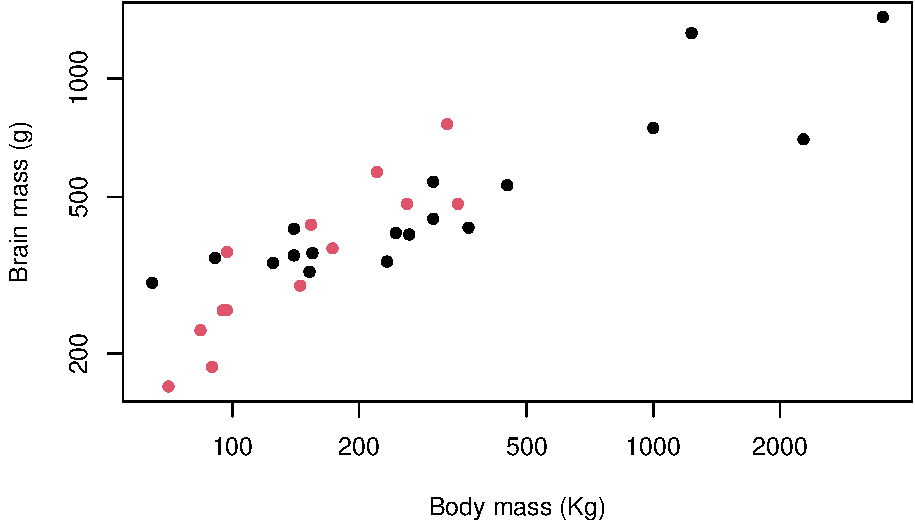
\includegraphics{3rd_Edition_files/figure-latex/graph11-1.pdf}
\caption{\label{fig:graph11}Brain mass versus body mass for 33 species of male pinniped plotted on log scaled axes, colour coded for mating system}
\end{figure}

That doesn't look too bad but you might not want to use it for a presentation or a publication. The default R palette has something of a bad reputation and the potential combinations of bright red, green and blue is enough to give most people a headache, not to mention the possible problems for people with red-green colourblindness. There will be a new and less offensive default palette \href{https://developer.r-project.org/Blog/public/2019/11/21/a-new-palette-for-r/index.html}{coming to R soon} but at the time of writing this hasn't been implemented yet. The good news though is that there are a lot of other palettes now available in a base R installation as part of the grDevices package, and there are also some really nice ones available as installable packages. The \texttt{ncl.pals()} function will give you a list of what's available in your base installation so long as it's a fairly recent one.

\begin{Shaded}
\begin{Highlighting}[]
\KeywordTok{hcl.pals}\NormalTok{()}
\NormalTok{  [}\DecValTok{1}\NormalTok{] }\StringTok{"Pastel 1"}      \StringTok{"Dark 2"}        \StringTok{"Dark 3"}        \StringTok{"Set 2"}        
\NormalTok{  [}\DecValTok{5}\NormalTok{] }\StringTok{"Set 3"}         \StringTok{"Warm"}          \StringTok{"Cold"}          \StringTok{"Harmonic"}     
\NormalTok{  [}\DecValTok{9}\NormalTok{] }\StringTok{"Dynamic"}       \StringTok{"Grays"}         \StringTok{"Light Grays"}   \StringTok{"Blues 2"}      
\NormalTok{ [}\DecValTok{13}\NormalTok{] }\StringTok{"Blues 3"}       \StringTok{"Purples 2"}     \StringTok{"Purples 3"}     \StringTok{"Reds 2"}       
\NormalTok{ [}\DecValTok{17}\NormalTok{] }\StringTok{"Reds 3"}        \StringTok{"Greens 2"}      \StringTok{"Greens 3"}      \StringTok{"Oslo"}         
\NormalTok{ [}\DecValTok{21}\NormalTok{] }\StringTok{"Purple-Blue"}   \StringTok{"Red-Purple"}    \StringTok{"Red-Blue"}      \StringTok{"Purple-Orange"}
\NormalTok{ [}\DecValTok{25}\NormalTok{] }\StringTok{"Purple-Yellow"} \StringTok{"Blue-Yellow"}   \StringTok{"Green-Yellow"}  \StringTok{"Red-Yellow"}   
\NormalTok{ [}\DecValTok{29}\NormalTok{] }\StringTok{"Heat"}          \StringTok{"Heat 2"}        \StringTok{"Terrain"}       \StringTok{"Terrain 2"}    
\NormalTok{ [}\DecValTok{33}\NormalTok{] }\StringTok{"Viridis"}       \StringTok{"Plasma"}        \StringTok{"Inferno"}       \StringTok{"Dark Mint"}    
\NormalTok{ [}\DecValTok{37}\NormalTok{] }\StringTok{"Mint"}          \StringTok{"BluGrn"}        \StringTok{"Teal"}          \StringTok{"TealGrn"}      
\NormalTok{ [}\DecValTok{41}\NormalTok{] }\StringTok{"Emrld"}         \StringTok{"BluYl"}         \StringTok{"ag_GrnYl"}      \StringTok{"Peach"}        
\NormalTok{ [}\DecValTok{45}\NormalTok{] }\StringTok{"PinkYl"}        \StringTok{"Burg"}          \StringTok{"BurgYl"}        \StringTok{"RedOr"}        
\NormalTok{ [}\DecValTok{49}\NormalTok{] }\StringTok{"OrYel"}         \StringTok{"Purp"}          \StringTok{"PurpOr"}        \StringTok{"Sunset"}       
\NormalTok{ [}\DecValTok{53}\NormalTok{] }\StringTok{"Magenta"}       \StringTok{"SunsetDark"}    \StringTok{"ag_Sunset"}     \StringTok{"BrwnYl"}       
\NormalTok{ [}\DecValTok{57}\NormalTok{] }\StringTok{"YlOrRd"}        \StringTok{"YlOrBr"}        \StringTok{"OrRd"}          \StringTok{"Oranges"}      
\NormalTok{ [}\DecValTok{61}\NormalTok{] }\StringTok{"YlGn"}          \StringTok{"YlGnBu"}        \StringTok{"Reds"}          \StringTok{"RdPu"}         
\NormalTok{ [}\DecValTok{65}\NormalTok{] }\StringTok{"PuRd"}          \StringTok{"Purples"}       \StringTok{"PuBuGn"}        \StringTok{"PuBu"}         
\NormalTok{ [}\DecValTok{69}\NormalTok{] }\StringTok{"Greens"}        \StringTok{"BuGn"}          \StringTok{"GnBu"}          \StringTok{"BuPu"}         
\NormalTok{ [}\DecValTok{73}\NormalTok{] }\StringTok{"Blues"}         \StringTok{"Lajolla"}       \StringTok{"Turku"}         \StringTok{"Blue-Red"}     
\NormalTok{ [}\DecValTok{77}\NormalTok{] }\StringTok{"Blue-Red 2"}    \StringTok{"Blue-Red 3"}    \StringTok{"Red-Green"}     \StringTok{"Purple-Green"} 
\NormalTok{ [}\DecValTok{81}\NormalTok{] }\StringTok{"Purple-Brown"}  \StringTok{"Green-Brown"}   \StringTok{"Blue-Yellow 2"} \StringTok{"Blue-Yellow 3"}
\NormalTok{ [}\DecValTok{85}\NormalTok{] }\StringTok{"Green-Orange"}  \StringTok{"Cyan-Magenta"}  \StringTok{"Tropic"}        \StringTok{"Broc"}         
\NormalTok{ [}\DecValTok{89}\NormalTok{] }\StringTok{"Cork"}          \StringTok{"Vik"}           \StringTok{"Berlin"}        \StringTok{"Lisbon"}       
\NormalTok{ [}\DecValTok{93}\NormalTok{] }\StringTok{"Tofino"}        \StringTok{"ArmyRose"}      \StringTok{"Earth"}         \StringTok{"Fall"}         
\NormalTok{ [}\DecValTok{97}\NormalTok{] }\StringTok{"Geyser"}        \StringTok{"TealRose"}      \StringTok{"Temps"}         \StringTok{"PuOr"}         
\NormalTok{[}\DecValTok{101}\NormalTok{] }\StringTok{"RdBu"}          \StringTok{"RdGy"}          \StringTok{"PiYG"}          \StringTok{"PRGn"}         
\NormalTok{[}\DecValTok{105}\NormalTok{] }\StringTok{"BrBG"}          \StringTok{"RdYlBu"}        \StringTok{"RdYlGn"}        \StringTok{"Spectral"}     
\NormalTok{[}\DecValTok{109}\NormalTok{] }\StringTok{"Zissou 1"}      \StringTok{"Cividis"}      
\end{Highlighting}
\end{Shaded}

This long list is in fact an implementation of the colour palettes available in the \href{https://cran.r-project.org/web/packages/colorspace/vignettes/colorspace.html}{colorspace} package for R, and these are themselves a mix of palettes from a variety of sources: for example the \texttt{Viridis} palette is from the eponymous \href{https://cran.r-project.org/web/packages/viridis/vignettes/intro-to-viridis.html}{Viridis} package.

I personally find a lot of these built-in colour palettes to be rather uninspiring and I prefer to use palettes from the \texttt{RColorBrewer} package. \texttt{RColorBrewer} gives you an R implementation of the palettes available on the \href{http://colorbrewer2.org/}{Color Brewer} website. The website is oriented towards cartographers but the palettes are useful for all sorts of data visualisations. The package will need to be installed if you don't already have it so you'd need to run \texttt{install.packages("RColorBrewer")}.

The palettes in \texttt{RColorBrewer} and elsewhere are usually grouped into ``sequential'', ``diverging'' and ``qualitative'' palettes. Sequential ones are suited for data on an ordered scale and tend to have a single underlying colour which is presented at varying degrees of lightness. Here are the available palettes from \texttt{RColorBrewer}:

\begin{Shaded}
\begin{Highlighting}[]
\KeywordTok{library}\NormalTok{(RColorBrewer)}
\KeywordTok{display.brewer.all}\NormalTok{(}\DataTypeTok{type =} \StringTok{"seq"}\NormalTok{)}
\end{Highlighting}
\end{Shaded}

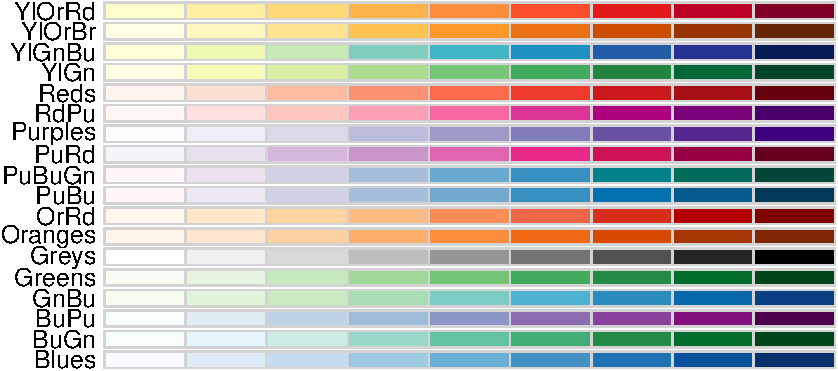
\includegraphics{3rd_Edition_files/figure-latex/unnamed-chunk-228-1.pdf}

Diverging palettes, like the sequential ones are suited for data where there is some sort of order but these palettes have contrasting colours for high and low values and (usually) pale shades for mid-range values.

\begin{Shaded}
\begin{Highlighting}[]
\KeywordTok{display.brewer.all}\NormalTok{(}\DataTypeTok{type =} \StringTok{"div"}\NormalTok{)}
\end{Highlighting}
\end{Shaded}

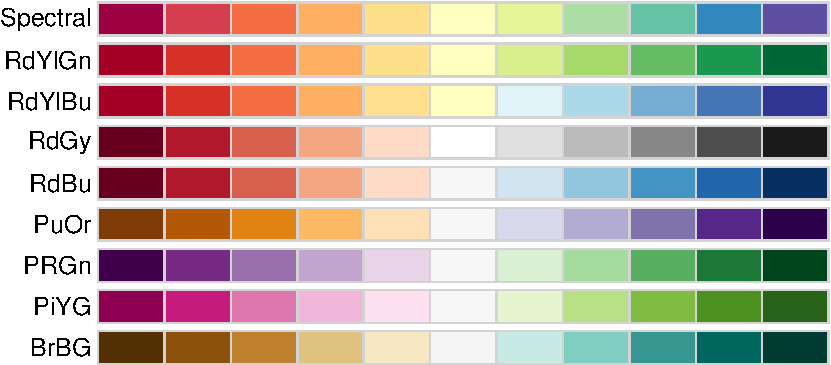
\includegraphics{3rd_Edition_files/figure-latex/unnamed-chunk-229-1.pdf}

Finally, qualitative palettes do not have any implied ordering and are best for representing data where the differences between data points are themselves not ordered.

\begin{Shaded}
\begin{Highlighting}[]
\KeywordTok{display.brewer.all}\NormalTok{(}\DataTypeTok{type =} \StringTok{"qual"}\NormalTok{)}
\end{Highlighting}
\end{Shaded}

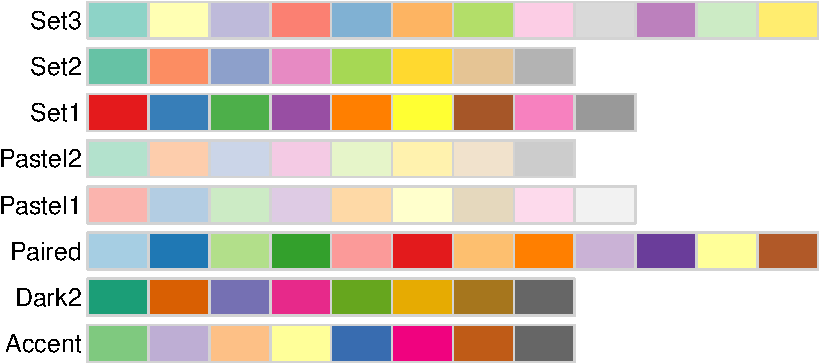
\includegraphics{3rd_Edition_files/figure-latex/unnamed-chunk-230-1.pdf}

These palettes have a variety of numbers of colours, and chances are that you'll want to use a different number from the default. You can't use more than the maximum, but you can easily generate and visualise sub-palettes with fewer colours present. As an example, if you wanted a palette based on the Dark2 palette but with seven colours only you can use the \texttt{display.brewer.pal()} function to visualise it and the \texttt{brewer.pal()} function to generate a new object with the appropriate hex codes.

\begin{Shaded}
\begin{Highlighting}[]
\KeywordTok{display.brewer.pal}\NormalTok{(}\DataTypeTok{n =} \DecValTok{7}\NormalTok{, }\DataTypeTok{name =} \StringTok{'Dark2'}\NormalTok{)}
\end{Highlighting}
\end{Shaded}

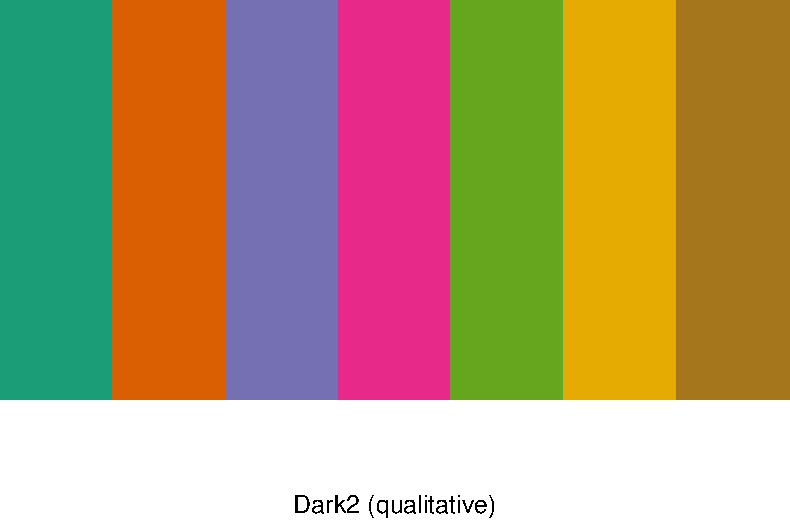
\includegraphics{3rd_Edition_files/figure-latex/unnamed-chunk-231-1.pdf}

\begin{Shaded}
\begin{Highlighting}[]
\NormalTok{palette1 <-}\StringTok{ }\KeywordTok{brewer.pal}\NormalTok{(}\DataTypeTok{n=}\DecValTok{7}\NormalTok{, }\DataTypeTok{name =} \StringTok{"Dark2"}\NormalTok{)}
\end{Highlighting}
\end{Shaded}

giving us a character vector called \texttt{palette1} with seven elements which are the hex codes for our colours.

\begin{Shaded}
\begin{Highlighting}[]
\NormalTok{palette1}
\NormalTok{[}\DecValTok{1}\NormalTok{] }\StringTok{"#1B9E77"} \StringTok{"#D95F02"} \StringTok{"#7570B3"} \StringTok{"#E7298A"} \StringTok{"#66A61E"} \StringTok{"#E6AB02"} \StringTok{"#A6761D"}
\end{Highlighting}
\end{Shaded}

Let's use this palette to plot a graph. The World\_bank\_data\_2014.csv dataset contains a wide variety of data on economics and development measured in 2014 for 186 countries around the World, as published by the \href{https://data.worldbank.org/}{World Bank}. Two variables are the percentage of the surface area which are classified as forested (\texttt{Forest\_area}) and the annual rainfall in mm (\texttt{Precipitation}). Let's plot these out, and colour code our data points by region (which happens to have seven values\ldots)

First of all we need to load the data. I'm running R4.0 so I'll need to specify the variables that I'd like to use as factors.

\begin{Shaded}
\begin{Highlighting}[]

\NormalTok{WB <-}\StringTok{ }\KeywordTok{read.csv}\NormalTok{(}\StringTok{"http://www.introductoryr.co.uk/World_bank_data_2014.csv"}\NormalTok{)}
\NormalTok{WB}\OperatorTok{$}\NormalTok{Region <-}\StringTok{ }\KeywordTok{as.factor}\NormalTok{(WB}\OperatorTok{$}\NormalTok{Region)}
\NormalTok{WB}\OperatorTok{$}\NormalTok{Income_group <-}\StringTok{ }\KeywordTok{as.factor}\NormalTok{(WB}\OperatorTok{$}\NormalTok{Income_group)}

\KeywordTok{str}\NormalTok{(WB)}
\StringTok{'data.frame'}\OperatorTok{:}\StringTok{   }\DecValTok{186}\NormalTok{ obs. of  }\DecValTok{22}\NormalTok{ variables}\OperatorTok{:}
\StringTok{ }\ErrorTok{$}\StringTok{ }\NormalTok{Country_Name              }\OperatorTok{:}\StringTok{ }\NormalTok{chr  }\StringTok{"Afghanistan"} \StringTok{"Angola"} \StringTok{"Albania"} \StringTok{"Andorra"}\NormalTok{ ...}
 \OperatorTok{$}\StringTok{ }\NormalTok{Country_Code              }\OperatorTok{:}\StringTok{ }\NormalTok{chr  }\StringTok{"AFG"} \StringTok{"AGO"} \StringTok{"ALB"} \StringTok{"AND"}\NormalTok{ ...}
 \OperatorTok{$}\StringTok{ }\NormalTok{Region                    }\OperatorTok{:}\StringTok{ }\NormalTok{Factor w}\OperatorTok{/}\StringTok{ }\DecValTok{7}\NormalTok{ levels }\StringTok{"East Asia & Pacific"}\NormalTok{,..}\OperatorTok{:}\StringTok{ }\DecValTok{6} \DecValTok{7} \DecValTok{2} \DecValTok{2} \DecValTok{4} \DecValTok{3} \DecValTok{2} \DecValTok{3} \DecValTok{1} \DecValTok{2}\NormalTok{ ...}
 \OperatorTok{$}\StringTok{ }\NormalTok{Income_group              }\OperatorTok{:}\StringTok{ }\NormalTok{Factor w}\OperatorTok{/}\StringTok{ }\DecValTok{4}\NormalTok{ levels }\StringTok{"High income"}\NormalTok{,..}\OperatorTok{:}\StringTok{ }\DecValTok{2} \DecValTok{3} \DecValTok{4} \DecValTok{1} \DecValTok{1} \DecValTok{4} \DecValTok{4} \DecValTok{1} \DecValTok{1} \DecValTok{1}\NormalTok{ ...}
 \OperatorTok{$}\StringTok{ }\NormalTok{Population                }\OperatorTok{:}\StringTok{ }\NormalTok{int  }\DecValTok{33370794} \DecValTok{26941779} \DecValTok{2889104} \DecValTok{79213} \DecValTok{9214175} \DecValTok{42669500} \DecValTok{2912403} \DecValTok{92562} \DecValTok{23475686} \DecValTok{8546356}\NormalTok{ ...}
 \OperatorTok{$}\StringTok{ }\NormalTok{Land_area                 }\OperatorTok{:}\StringTok{ }\NormalTok{num  }\DecValTok{652860} \DecValTok{1246700} \DecValTok{27400} \DecValTok{470} \DecValTok{71020}\NormalTok{ ...}
 \OperatorTok{$}\StringTok{ }\NormalTok{Forest_area               }\OperatorTok{:}\StringTok{ }\NormalTok{num  }\FloatTok{2.07} \FloatTok{46.51} \FloatTok{28.19} \FloatTok{34.04} \FloatTok{4.53}\NormalTok{ ...}
 \OperatorTok{$}\StringTok{ }\NormalTok{Precipitation             }\OperatorTok{:}\StringTok{ }\NormalTok{int  }\DecValTok{327} \DecValTok{1010} \DecValTok{1485} \OtherTok{NA} \DecValTok{78} \DecValTok{591} \DecValTok{562} \DecValTok{1030} \DecValTok{534} \DecValTok{1110}\NormalTok{ ...}
 \OperatorTok{$}\StringTok{ }\NormalTok{Population_density        }\OperatorTok{:}\StringTok{ }\NormalTok{num  }\FloatTok{51.1} \FloatTok{21.6} \FloatTok{105.4} \FloatTok{168.5} \FloatTok{129.7}\NormalTok{ ...}
 \OperatorTok{$}\StringTok{ }\NormalTok{Capital_lat               }\OperatorTok{:}\StringTok{ }\NormalTok{int  }\DecValTok{33} \DecValTok{-13} \DecValTok{41} \DecValTok{43} \DecValTok{24} \DecValTok{-34} \DecValTok{40} \DecValTok{17} \DecValTok{-35} \DecValTok{47}\NormalTok{ ...}
 \OperatorTok{$}\StringTok{ }\NormalTok{GNP_per_Cap               }\OperatorTok{:}\StringTok{ }\NormalTok{int  }\DecValTok{630} \DecValTok{5010} \DecValTok{4540} \OtherTok{NA} \DecValTok{44330} \DecValTok{12350} \DecValTok{4140} \DecValTok{12730} \DecValTok{65150} \DecValTok{50370}\NormalTok{ ...}
 \OperatorTok{$}\StringTok{ }\NormalTok{Population_growth         }\OperatorTok{:}\StringTok{ }\NormalTok{num  }\FloatTok{3.356} \FloatTok{3.497} \FloatTok{-0.207} \FloatTok{-1.951} \FloatTok{0.177}\NormalTok{ ...}
 \OperatorTok{$}\StringTok{ }\NormalTok{Cereal_yield              }\OperatorTok{:}\StringTok{ }\NormalTok{num  }\DecValTok{2018} \DecValTok{888} \DecValTok{4893} \OtherTok{NA} \DecValTok{12543}\NormalTok{ ...}
 \OperatorTok{$}\StringTok{ }\NormalTok{Under_}\DecValTok{5}\NormalTok{_mortality         }\OperatorTok{:}\StringTok{ }\NormalTok{num  }\FloatTok{73.6} \FloatTok{92.9} \DecValTok{10} \FloatTok{3.4} \FloatTok{7.9} \DecValTok{12} \FloatTok{15.1} \FloatTok{7.6} \DecValTok{4} \FloatTok{3.8}\NormalTok{ ...}
 \OperatorTok{$}\StringTok{ }\NormalTok{Renewables                }\OperatorTok{:}\StringTok{ }\NormalTok{num  }\FloatTok{19.314} \FloatTok{50.797} \FloatTok{38.69} \FloatTok{19.886} \FloatTok{0.146}\NormalTok{ ...}
 \OperatorTok{$}\StringTok{ }\NormalTok{CO2                       }\OperatorTok{:}\StringTok{ }\NormalTok{num  }\FloatTok{0.294} \FloatTok{1.29} \FloatTok{1.979} \FloatTok{5.833} \FloatTok{22.94}\NormalTok{ ...}
 \OperatorTok{$}\StringTok{ }\NormalTok{PM25                      }\OperatorTok{:}\StringTok{ }\NormalTok{num  }\DecValTok{59} \DecValTok{33} \FloatTok{18.9} \FloatTok{10.8} \DecValTok{38}\NormalTok{ ...}
 \OperatorTok{$}\StringTok{ }\NormalTok{Women_in_parliament       }\OperatorTok{:}\StringTok{ }\NormalTok{num  }\FloatTok{27.7} \FloatTok{36.8} \DecValTok{20} \DecValTok{50} \FloatTok{17.5} \FloatTok{36.6} \FloatTok{10.7} \FloatTok{11.1} \DecValTok{26} \FloatTok{32.2}\NormalTok{ ...}
 \OperatorTok{$}\StringTok{ }\NormalTok{GINI_index                }\OperatorTok{:}\StringTok{ }\NormalTok{num  }\OtherTok{NA} \OtherTok{NA} \OtherTok{NA} \OtherTok{NA} \OtherTok{NA} \FloatTok{41.7} \FloatTok{31.5} \OtherTok{NA} \FloatTok{35.8} \FloatTok{30.5}\NormalTok{ ...}
 \OperatorTok{$}\StringTok{ }\NormalTok{Govt_spend_education      }\OperatorTok{:}\StringTok{ }\NormalTok{num  }\FloatTok{3.7} \OtherTok{NA} \OtherTok{NA} \DecValTok{3} \OtherTok{NA}\NormalTok{ ...}
 \OperatorTok{$}\StringTok{ }\NormalTok{Secondary_school_enrolment}\OperatorTok{:}\StringTok{ }\NormalTok{num  }\FloatTok{52.6} \OtherTok{NA} \FloatTok{97.7} \OtherTok{NA} \OtherTok{NA}\NormalTok{ ...}
 \OperatorTok{$}\StringTok{ }\NormalTok{School_gender_parity      }\OperatorTok{:}\StringTok{ }\NormalTok{num  }\FloatTok{0.654} \OtherTok{NA} \FloatTok{0.977} \OtherTok{NA} \OtherTok{NA}\NormalTok{ ...}
\end{Highlighting}
\end{Shaded}

Now that we have our data a little housekeeping is in order. We're going to want to add a legend ot our plot in the right hand margin so we need to adjust the sizes of the figure margins using \texttt{par(mar\ =\ c(5,4,4,12))}. The vector of numbers is the size of the margins in the order of bottom, left, top, right and it would normally be set at \texttt{c(5,4,4,2)\ +\ 0.1} so we're making the right hand margin much bigger than it would normally be.

\texttt{par(xpd\ =\ TRUE)} sets R so that we can plot our legend in the margin: normally in base graphics it would be restricted to inside the plotting area.

Now that we've done that we can plot our graph, add the legend and then finally set our two parameters back to their default values. It's always a good idea to do this because if you don't then you'll inevitably forget and then you'll end up wondering why your graph looks odd.

\begin{Shaded}
\begin{Highlighting}[]

\KeywordTok{par}\NormalTok{(}\DataTypeTok{mar =} \KeywordTok{c}\NormalTok{(}\DecValTok{5}\NormalTok{,}\DecValTok{4}\NormalTok{,}\DecValTok{4}\NormalTok{,}\DecValTok{13}\NormalTok{))}
\KeywordTok{par}\NormalTok{(}\DataTypeTok{xpd =} \OtherTok{TRUE}\NormalTok{)}

\KeywordTok{plot}\NormalTok{(WB}\OperatorTok{$}\NormalTok{Forest_area }\OperatorTok{~}\StringTok{ }\NormalTok{WB}\OperatorTok{$}\NormalTok{Precipitation, }
     \DataTypeTok{col =}\NormalTok{ palette1[WB}\OperatorTok{$}\NormalTok{Region], }
     \DataTypeTok{pch =} \DecValTok{16}\NormalTok{,}
     \DataTypeTok{xlab =} \StringTok{"Precipitation (mm per year)"}\NormalTok{,}
     \DataTypeTok{ylab =} \StringTok{"Forest area (%)"}\NormalTok{)}

\KeywordTok{legend}\NormalTok{(}\DataTypeTok{x=}\DecValTok{3500}\NormalTok{, }\DataTypeTok{y=}\DecValTok{80}\NormalTok{, }
       \DataTypeTok{col =}\NormalTok{ palette1, }
       \DataTypeTok{pch =} \DecValTok{16}\NormalTok{, }
       \DataTypeTok{legend =} \KeywordTok{levels}\NormalTok{(WB}\OperatorTok{$}\NormalTok{Region), }
       \DataTypeTok{bty =} \StringTok{"n"}\NormalTok{, }
       \DataTypeTok{title =} \StringTok{"Region"}\NormalTok{)}

\KeywordTok{par}\NormalTok{(}\DataTypeTok{mar =} \KeywordTok{c}\NormalTok{(}\DecValTok{5}\NormalTok{,}\DecValTok{4}\NormalTok{,}\DecValTok{4}\NormalTok{,}\DecValTok{2}\NormalTok{) }\OperatorTok{+}\StringTok{ }\FloatTok{0.1}\NormalTok{)}
\KeywordTok{par}\NormalTok{(}\DataTypeTok{xpd =} \OtherTok{FALSE}\NormalTok{)}
\end{Highlighting}
\end{Shaded}

Before we look at our final plot, let's just run through those \texttt{plot()} and \texttt{legend()} function calls and see what all the arguments do.

\begin{Shaded}
\begin{Highlighting}[]
\KeywordTok{plot}\NormalTok{(WB}\OperatorTok{$}\NormalTok{Forest_area }\OperatorTok{~}\StringTok{ }\NormalTok{WB}\OperatorTok{$}\NormalTok{Precipitation, }
     \DataTypeTok{col =}\NormalTok{ palette1[WB}\OperatorTok{$}\NormalTok{Region], }
     \DataTypeTok{pch =} \DecValTok{16}\NormalTok{,}
     \DataTypeTok{xlab =} \StringTok{"Precipitation (mm per year)"}\NormalTok{,}
     \DataTypeTok{ylab =} \StringTok{"Forest area (%)"}\NormalTok{)}
\end{Highlighting}
\end{Shaded}

This is the function call that plots the graph. We start off by giving \texttt{plot()} the names of two continuous variables (\texttt{Forest\_area} and \texttt{Precipitation}), both from the \texttt{WB} data frame. These are separated by a tilde \texttt{\textasciitilde{}} which means ``the one on the left of the tilde as explained by the one on the right''\ldots{} so \texttt{plot()} will draw us a scatterplot with \texttt{Forest\_area} on the y-axis and \texttt{Precipitation} on the x-axis.

Next comes \texttt{col\ =\ palette1{[}WB\$Region{]},} which determines the colours used in the plot. We've already set up \texttt{palette1} which is a vector of seven colours derived from the RColorBrewer Dark2 palette. Using the factor \texttt{Region} from the \texttt{WB} data frame as a subscript generates a vector of colours corresponding to the factor levels, as we saw above. Finally we have three fairly simple arguments. \texttt{pch\ =\ 16} sets the plot symbol to be a filled circle, and \texttt{xlab\ =} and \texttt{ylab\ =} set the two axis labels.

This plots our graph. Moving on to the \texttt{legend()} function call, this is one of a number of R functions which you can use to draw things like lines, text or more data on to an existing graph and we'll discuss these in detail in the next chapter. For the moment, I'll just quickly run you thorugh what the various arguments are doing.

\begin{Shaded}
\begin{Highlighting}[]
\KeywordTok{legend}\NormalTok{(}\DataTypeTok{x=}\DecValTok{3500}\NormalTok{, }\DataTypeTok{y=}\DecValTok{80}\NormalTok{, }
       \DataTypeTok{col =}\NormalTok{ palette1, }
       \DataTypeTok{pch =} \DecValTok{16}\NormalTok{, }
       \DataTypeTok{legend =} \KeywordTok{levels}\NormalTok{(WB}\OperatorTok{$}\NormalTok{Region), }
       \DataTypeTok{bty =} \StringTok{"n"}\NormalTok{, }
       \DataTypeTok{title =} \StringTok{"Region"}\NormalTok{)}
\end{Highlighting}
\end{Shaded}

The \texttt{x=3500,\ y=80} arguments are telling R where to put the top left corner of the legend. The units are the same as those that the graph is plotted in, which makes life a bit easier. Note that 3500 is outside the range of the x-axis, so we're asking R to plot the legend next to the graph rather than inside the graph box, which is why we have to set \texttt{par(xpd\ =\ TRUE)}.

\texttt{col\ =\ palette1} tells \texttt{legend()} which colours to include, and \texttt{pch\ =\ 16} tells it which plot symbol to use. \texttt{legend\ =\ levels(WB\$Region)} is the code which tells \texttt{legend()} what text to use. In this case the \texttt{levels()} function will give us the names of the levels of the \texttt{WB\$Region} factor, and this is the information we'd like on the legend. Two final arguments are \texttt{bty\ =\ "n"} --- \texttt{bty} stands for ``box type'' and setting this to ``n'' means that there isn't a box drawn around the legend, and finally \texttt{title\ =\ "Region"} specifies a title for the legend.

Here's the final graph:

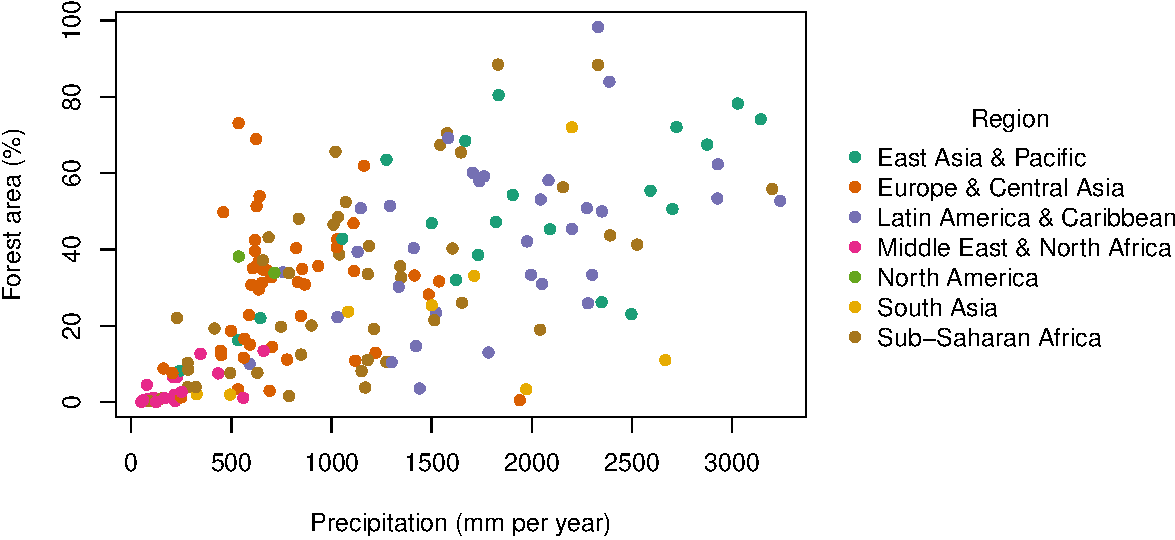
\includegraphics{3rd_Edition_files/figure-latex/unnamed-chunk-238-1.pdf}

This is an interesting graph. You can see that there is a strong but messy relationship between total precipitation and forest cover, so almost all of the nations with high forest cover also have relatively high precipitation. There are, however, some nations with high precipitation but rather low forest cover. The colour coding lets us see which regions fall where on this graph, so high ofrest cover and high precipitation nations are mostly from the East Asia \& Pacific and Latin America \& Caribbean regions. The Middle East and North Africa has, of course, a lot of desert and a generally very low rainfall and these nations can all be seen clustering close to the origin.

\hypertarget{using-transparency-in-your-graphs}{%
\section{Using transparency in your graphs}\label{using-transparency-in-your-graphs}}

Something that you can do if you wish to dip your toe into the waters of hexadecimal colour coding is use colours which are transparent, so parts of the graph that are plotted underneath them can show through. This can be useful if, for example, you wish to produce a figure with two histograms plotted on top of each other so that the shapes of two frequency distributions can be compared. We can illustrate this with some results data from the 2012 Ironman Triathlon World Championship in Hawaii. This is a race in which the participants swim for 3.8km, cycle for 180km and then run a marathon. We'll look at these data again in the chapter on correlation, but for the moment we'll look at the relationship between swim times and bike times for all competitors.

\begin{Shaded}
\begin{Highlighting}[]
\NormalTok{IMH<-}\KeywordTok{read.table}\NormalTok{(}\StringTok{"http://www.introductoryr.co.uk/IMH2012.txt"}\NormalTok{)}
\KeywordTok{str}\NormalTok{(IMH)}
\StringTok{'data.frame'}\OperatorTok{:}\StringTok{   }\DecValTok{1879}\NormalTok{ obs. of  }\DecValTok{6}\NormalTok{ variables}\OperatorTok{:}
\StringTok{ }\ErrorTok{$}\StringTok{ }\NormalTok{Gender  }\OperatorTok{:}\StringTok{ }\NormalTok{chr  }\StringTok{"M"} \StringTok{"M"} \StringTok{"M"} \StringTok{"M"}\NormalTok{ ...}
 \OperatorTok{$}\StringTok{ }\NormalTok{Category}\OperatorTok{:}\StringTok{ }\NormalTok{chr  }\StringTok{"PRO"} \StringTok{"PRO"} \StringTok{"PRO"} \StringTok{"PRO"}\NormalTok{ ...}
 \OperatorTok{$}\StringTok{ }\NormalTok{Swim    }\OperatorTok{:}\StringTok{ }\NormalTok{num  }\FloatTok{0.858} \FloatTok{0.921} \FloatTok{0.86} \FloatTok{0.922} \FloatTok{0.861}\NormalTok{ ...}
 \OperatorTok{$}\StringTok{ }\NormalTok{Bike    }\OperatorTok{:}\StringTok{ }\NormalTok{num  }\FloatTok{4.59} \FloatTok{4.61} \FloatTok{4.59} \FloatTok{4.56} \FloatTok{4.6}\NormalTok{ ...}
 \OperatorTok{$}\StringTok{ }\NormalTok{Run     }\OperatorTok{:}\StringTok{ }\NormalTok{num  }\FloatTok{2.8} \FloatTok{2.79} \FloatTok{2.88} \FloatTok{2.91} \FloatTok{2.95}\NormalTok{ ...}
 \OperatorTok{$}\StringTok{ }\NormalTok{Overall }\OperatorTok{:}\StringTok{ }\NormalTok{num  }\FloatTok{8.31} \FloatTok{8.39} \FloatTok{8.4} \FloatTok{8.45} \FloatTok{8.48}\NormalTok{ ...}
\end{Highlighting}
\end{Shaded}

\begin{Shaded}
\begin{Highlighting}[]
\KeywordTok{plot}\NormalTok{(}
\NormalTok{  IMH}\OperatorTok{$}\NormalTok{Swim,}
\NormalTok{  IMH}\OperatorTok{$}\NormalTok{Bike,}
  \DataTypeTok{pch =} \DecValTok{16}\NormalTok{,}
  \DataTypeTok{col =} \StringTok{"aquamarine4"}\NormalTok{,}
  \DataTypeTok{xlab =} \StringTok{"Swim split (hours)"}\NormalTok{,}
  \DataTypeTok{ylab =} \StringTok{"Run split (hours)"}
\NormalTok{)}
\end{Highlighting}
\end{Shaded}

\begin{figure}
\centering
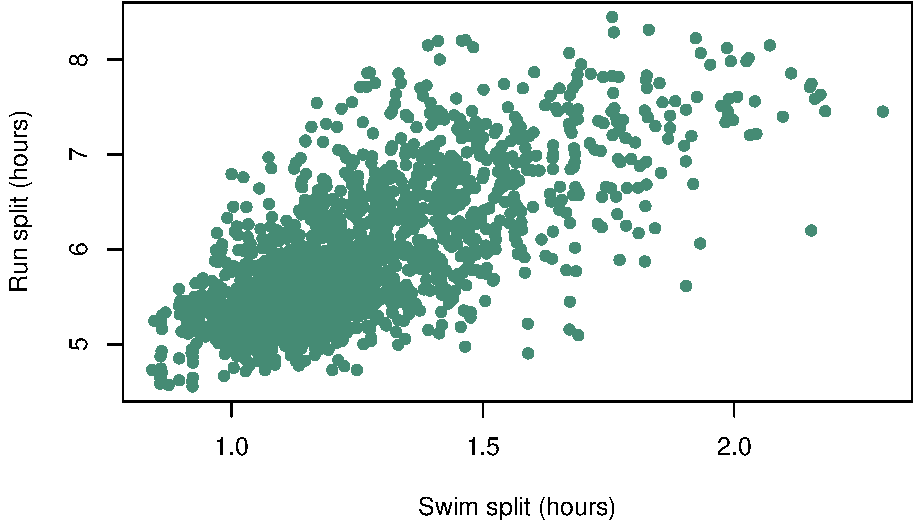
\includegraphics{3rd_Edition_files/figure-latex/unnamed-chunk-240-1.pdf}
\caption{\label{fig:unnamed-chunk-240}Run split plotted against bike split for each individual competitor at the 2012 Hawaii Ironman Triathlon.}
\end{figure}

We have lots of data points and they all plot on top of each other making it difficult to work out what the patterns in the data really are. If we add an element of transparency to those points it might make the graph easier to interpret.

To add transparency we need to find out the hexadecimal values for the colours we'd like to use, which we can find using a function called \texttt{col2rgb()}, which gives the RGB values for a named colour. We have to tell R that we want the values given as hexadecimal rather than base 10, which we do with the \texttt{as.hexmode()} function.

\begin{Shaded}
\begin{Highlighting}[]
\KeywordTok{as.hexmode}\NormalTok{(}\KeywordTok{col2rgb}\NormalTok{(}\StringTok{"aquamarine4"}\NormalTok{))}
\NormalTok{      [,}\DecValTok{1}\NormalTok{]}
\NormalTok{red   }\StringTok{"45"}
\NormalTok{green }\StringTok{"8b"}
\NormalTok{blue  }\StringTok{"74"}
\end{Highlighting}
\end{Shaded}

Our hexadecimal value for \emph{aquamarine4} is ``\#458b74''. To make this transparent we add an extra two digits to the right hand side of this number, which determine how see-through it will be. Low values mean that most of what is drawn below will show through, so if we gave this ``alpha channel'' number as 32 then 32/255 or 12.5\% of the top value will be seen. Alternatively, if we gave it as CC (the alpha channel is also specified in hexadecimal) then 204/255 or 80\% of the colour drawn on the top will be seen. We'll use 64 which means that roughly 25\% of the top colour will be used.

\begin{Shaded}
\begin{Highlighting}[]
\KeywordTok{plot}\NormalTok{(}
\NormalTok{  IMH}\OperatorTok{$}\NormalTok{Swim,}
\NormalTok{  IMH}\OperatorTok{$}\NormalTok{Bike,}
  \DataTypeTok{pch =} \DecValTok{16}\NormalTok{,}
  \DataTypeTok{col =} \StringTok{"#458b7464"}\NormalTok{,}
  \DataTypeTok{xlab =} \StringTok{"Swim split (hours)"}\NormalTok{,}
  \DataTypeTok{ylab =} \StringTok{"Bike split (hours)"}
\NormalTok{)}
\end{Highlighting}
\end{Shaded}

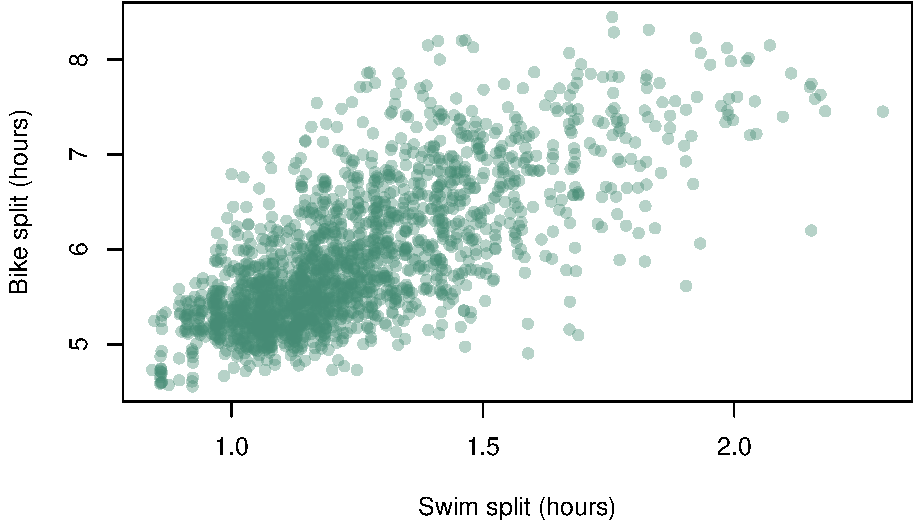
\includegraphics{3rd_Edition_files/figure-latex/unnamed-chunk-242-1.pdf}
This gives us a very different graph. Rather than the focus being on the overall shape of the point scatter we can now see some structure within, and the dense cluster of points in the lower left corner of the plot is much clearer.

\hypertarget{histograms-and-multiple-plots-in-the-same-window}{%
\section{Histograms and multiple plots in the same window}\label{histograms-and-multiple-plots-in-the-same-window}}

R doesn't only draw scatterplots, of course. When you have continuous data of any sort then you might well want to draw a \emph{frequency histogram} which will show the shape of the dataset. The R function which draws histograms is \texttt{hist()} and if you're just doing some exploratory analysis this is a super-speedy way of having a look at the shape of your data.

Here are two examples:

\begin{Shaded}
\begin{Highlighting}[]
\KeywordTok{par}\NormalTok{(}\DataTypeTok{mfrow =} \KeywordTok{c}\NormalTok{(}\DecValTok{1}\NormalTok{,}\DecValTok{2}\NormalTok{))}

\KeywordTok{hist}\NormalTok{(WB}\OperatorTok{$}\NormalTok{CO2, }
     \DataTypeTok{xlab =} \KeywordTok{expression}\NormalTok{(}\KeywordTok{paste}\NormalTok{(}\StringTok{"CO"}\NormalTok{[}\DecValTok{2}\NormalTok{], }\StringTok{" production per capita (tonnes)"}\NormalTok{)), }
     \DataTypeTok{main =} \StringTok{""}\NormalTok{)}

\KeywordTok{hist}\NormalTok{(WB}\OperatorTok{$}\NormalTok{Population_growth, }
     \DataTypeTok{xlab =} \StringTok{"Population growth (%)"}\NormalTok{, }
     \DataTypeTok{main =} \StringTok{""}\NormalTok{)}
\end{Highlighting}
\end{Shaded}

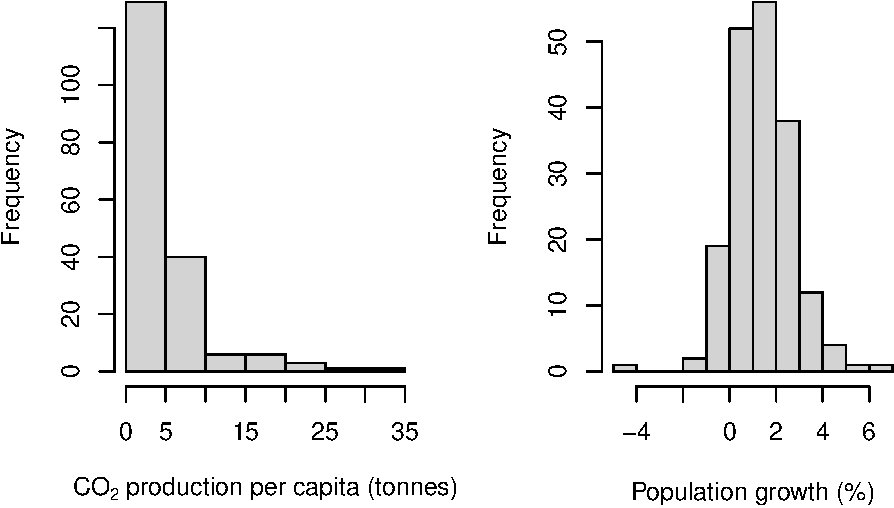
\includegraphics{3rd_Edition_files/figure-latex/unnamed-chunk-243-1.pdf}

\begin{Shaded}
\begin{Highlighting}[]

\KeywordTok{par}\NormalTok{(}\DataTypeTok{mfrow =} \KeywordTok{c}\NormalTok{(}\DecValTok{1}\NormalTok{,}\DecValTok{1}\NormalTok{))}
\end{Highlighting}
\end{Shaded}

I've introduced a couple of new things here in addition to the \texttt{hist()} function calls. Firstly there is the use of \texttt{par(mfrow\ =\ c(1,2))} as the first line of code. This allows us to draw more than one plot: the actual number is determined by the numbers that the paramter os set to. The first value (1 in this case) is the number of rows and the second is the number of columns: so here I'm telling R to give me a graphics device into which I can draw two plots side-by-side. \texttt{par(mfrow\ =\ c(2,1))} would give one above the other and \texttt{par(mfrow\ =\ c(2,2))} would give four plots arranged in a square. R will fill the graphics device in as new \texttt{plot()} or similar instructions arrive, so in this ase the first histogram goes on the left side and the second on the right. If we were to use a third \texttt{hist()} function R would clear the graphics device and draw the new one on the left, leaving the right hand slot blank.

Two important things must you know about setting the \texttt{mfrow} parameter to anything other than \texttt{c(1,1)}. Firstly, once you have plotted a second (or third\ldots) plot you cannot add anything more to the first (or second\ldots). So if you are planning to add a line or some text, or a legend (see the next chapter for details of how to do this), you have to do it \textbf{before} the next plot is drawn. Secondly, it's really good practice always to reset the parameter to \texttt{c(1,1)} whenever you've finished, otherwise you can just get in a mess.

ONe other thing that's new is the somewhat complex code the the x-axis label of the first histogram which is there to get the subscript in CO\textsubscript{2} this is a bit of a complex sunject and for the moment let's just say that without something like this it's difficult to get things like subscripts and mathematical symbols in axis labels. More in the next chapter.

Now that we've covered that, let's look at those histograms. We've fed R some continuous data, R has divided our data into a series of intervals (e.g.~intervals defined by 0,5,10,15,20 etc. for CO\textsubscript{2} production) and then counted the number of data points which fall into each interval. The number of intervals (or ``bins'' as they are usually called) is determined by an internal algorithm which is meant to find a good number to show the shape of the data, but you will often want to have more or fewer than the default option: as an example, in this case the algorithm has decided to have 12 bins for the population growth data but only 7 for the CO\textsubscript{2} production data despite the sample sizes being the same. If we wanted to have the same number of bins for both histograms we could use the \texttt{breaks\ =} argument to force \texttt{hist()} into drawing what we want. Here we're going to use the \texttt{seq()} function to generate 13 equally spaced values with the lowest being 0 and the highest 35. This will give us a histogram with 12 equally sized bins for CO\textsubscript{2} production.

We're also going to make the histograms look a little better by colouring the bars usng the \texttt{col\ =} parameter.

\begin{Shaded}
\begin{Highlighting}[]
\KeywordTok{par}\NormalTok{(}\DataTypeTok{mfrow =} \KeywordTok{c}\NormalTok{(}\DecValTok{1}\NormalTok{,}\DecValTok{2}\NormalTok{))}

\KeywordTok{hist}\NormalTok{(WB}\OperatorTok{$}\NormalTok{CO2,}
     \DataTypeTok{breaks =} \KeywordTok{seq}\NormalTok{(}\DataTypeTok{from =} \DecValTok{0}\NormalTok{, }\DataTypeTok{to =} \DecValTok{35}\NormalTok{, }\DataTypeTok{length =} \DecValTok{13}\NormalTok{),}
     \DataTypeTok{col =} \StringTok{"aquamarine4"}\NormalTok{,}
     \DataTypeTok{xlab =} \KeywordTok{expression}\NormalTok{(}\KeywordTok{paste}\NormalTok{(}\StringTok{"CO"}\NormalTok{[}\DecValTok{2}\NormalTok{], }\StringTok{" production per capita (tonnes)"}\NormalTok{)), }
     \DataTypeTok{main =} \StringTok{""}\NormalTok{)}

\KeywordTok{hist}\NormalTok{(WB}\OperatorTok{$}\NormalTok{Population_growth,}
     \DataTypeTok{col =} \StringTok{"aquamarine4"}\NormalTok{,}
     \DataTypeTok{xlab =} \StringTok{"Population growth (%)"}\NormalTok{, }
     \DataTypeTok{main =} \StringTok{""}\NormalTok{)}
\end{Highlighting}
\end{Shaded}

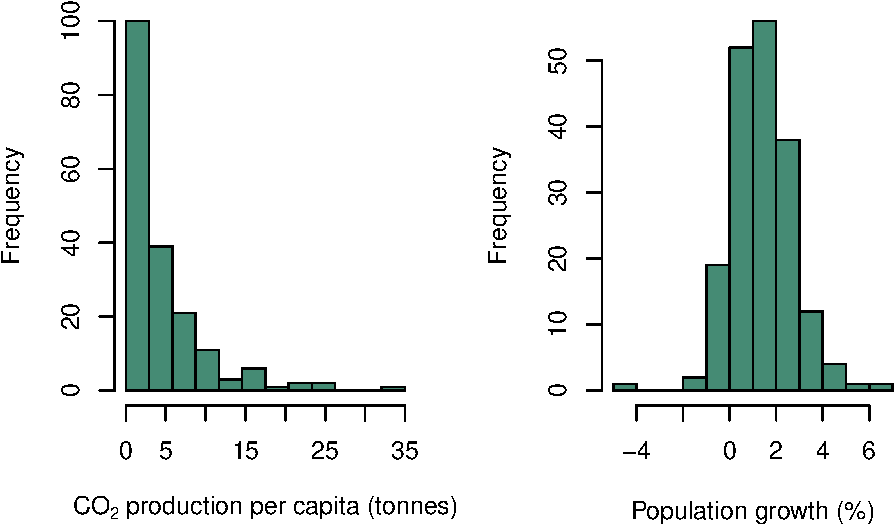
\includegraphics{3rd_Edition_files/figure-latex/unnamed-chunk-244-1.pdf}

\begin{Shaded}
\begin{Highlighting}[]

\KeywordTok{par}\NormalTok{(}\DataTypeTok{mfrow =} \KeywordTok{c}\NormalTok{(}\DecValTok{1}\NormalTok{,}\DecValTok{1}\NormalTok{))}
\end{Highlighting}
\end{Shaded}

The default option fot \texttt{hist()} is to draw a histogram showing the numbers in each bin. If you want what many people would regard as a \emph{true frequency histogram} then rather than the numbers for each bin you wuld want to plot the histogram with the frequencies nornalised to 1, so that the values for all bins summed together add up to 1. This can be done by setting the \texttt{freq\ =} argument to \texttt{FALSE}.

You can also draw histograms with bins of different widths if you want: let's say that you wanted to put all the countries with CO\textsubscript{2} production below 5 tonnes per year into a single bin, and then have the rest binned in intervals of 1 tonne each. Here's that histogram drawn with \texttt{freq\ =\ FALSE} so the \emph{area} of all the bars adds up to 1.

\begin{Shaded}
\begin{Highlighting}[]
\NormalTok{break1 <-}\StringTok{ }\KeywordTok{c}\NormalTok{(}\DecValTok{0}\NormalTok{, }\KeywordTok{seq}\NormalTok{(}\DataTypeTok{from =} \DecValTok{5}\NormalTok{, }\DataTypeTok{to =} \DecValTok{35}\NormalTok{, }\DataTypeTok{by =} \DecValTok{1}\NormalTok{))}

\KeywordTok{hist}\NormalTok{(WB}\OperatorTok{$}\NormalTok{CO2,}
     \DataTypeTok{breaks =}\NormalTok{ break1,}
     \DataTypeTok{freq =} \OtherTok{FALSE}\NormalTok{,}
     \DataTypeTok{col =} \StringTok{"steelblue"}\NormalTok{,}
     \DataTypeTok{xlab =} \KeywordTok{expression}\NormalTok{(}\KeywordTok{paste}\NormalTok{(}\StringTok{"CO"}\NormalTok{[}\DecValTok{2}\NormalTok{], }\StringTok{" production per capita (tonnes)"}\NormalTok{)), }
     \DataTypeTok{main =} \StringTok{""}\NormalTok{)}
\end{Highlighting}
\end{Shaded}

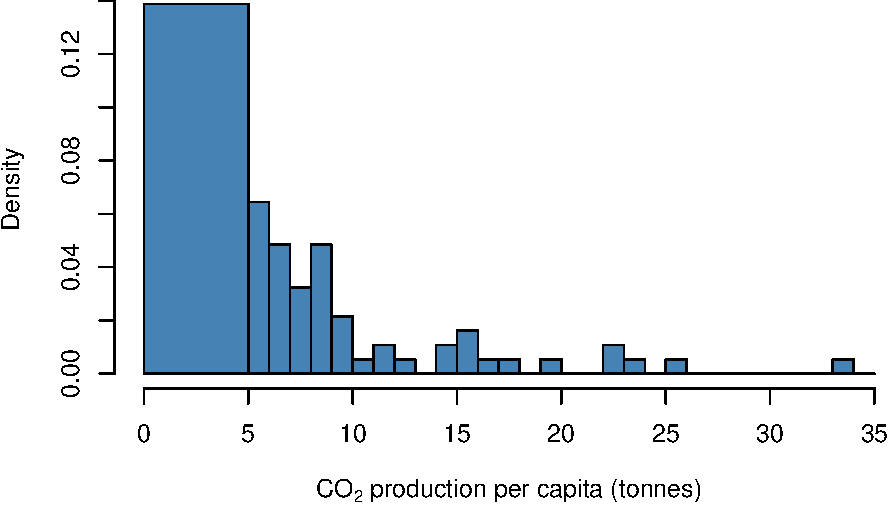
\includegraphics{3rd_Edition_files/figure-latex/unnamed-chunk-245-1.pdf}

\hypertarget{boxplots}{%
\section{Boxplots}\label{boxplots}}

One of the most useful and common types of graph is the \emph{boxplot} - a method of plotting data which shows not only the central tendency but also the amount of dispersion in your data. R can do this in one of two ways. Firstly, you can use the \texttt{boxplot()} function, which will draw either a boxplot of a single continuous variable or a continuous variable against the levels of a factor or even more than one factor.

Here are the boxplots corresponding to the CO\textsubscript{2} and population growth data which we drew some histograms of in the previous section.

\begin{Shaded}
\begin{Highlighting}[]
\KeywordTok{par}\NormalTok{(}\DataTypeTok{mfrow =} \KeywordTok{c}\NormalTok{(}\DecValTok{1}\NormalTok{,}\DecValTok{2}\NormalTok{))}

\KeywordTok{boxplot}\NormalTok{(WB}\OperatorTok{$}\NormalTok{CO2, }
        \DataTypeTok{ylab =} \KeywordTok{expression}\NormalTok{(}\KeywordTok{paste}\NormalTok{(}\StringTok{"CO"}\NormalTok{[}\DecValTok{2}\NormalTok{], }\StringTok{" production per capita (tonnes)"}\NormalTok{)))}

\KeywordTok{boxplot}\NormalTok{(WB}\OperatorTok{$}\NormalTok{Population_growth, }
        \DataTypeTok{ylab =} \StringTok{"Population growth (%)"}\NormalTok{)}
\end{Highlighting}
\end{Shaded}

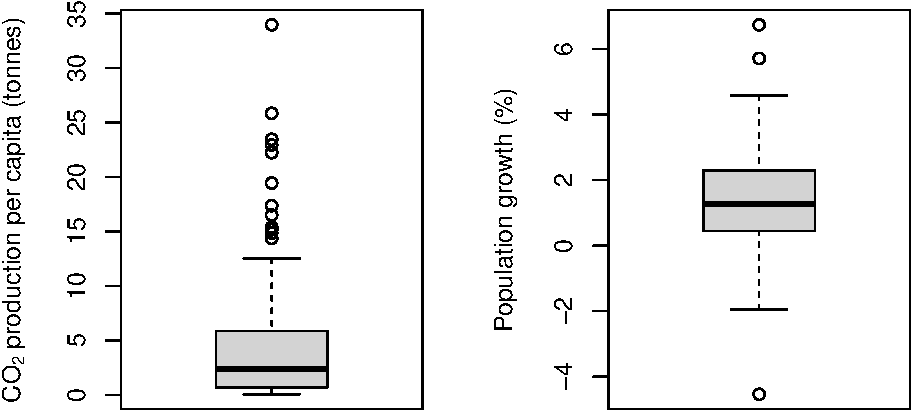
\includegraphics{3rd_Edition_files/figure-latex/unnamed-chunk-246-1.pdf}

\begin{Shaded}
\begin{Highlighting}[]

\KeywordTok{par}\NormalTok{(}\DataTypeTok{mfrow =} \KeywordTok{c}\NormalTok{(}\DecValTok{1}\NormalTok{,}\DecValTok{1}\NormalTok{))}
\end{Highlighting}
\end{Shaded}

One thing to note is that whereas \texttt{hist()} festoons its outputs with axis labels and titles to the point where you usually have to go out of your way to get rid of them, \texttt{boxplot()} has no truck with such tomfoolery and will only add these fripperies if you ask it to do so. Welcome to R.

If you've not seen a boxplot before they can be a little hard to understand, but they are a really good way to visualise the distribution of data in a particular variable. The heavy line is the \emph{median}, so it's telling you where the middle value is. The box shows the \emph{interquartile range} ----- the lower boundary is the 1st quartile, below which are the 25\% lowest data values, and the upper boundary is the 3rd quartile, above which are the 25\% highest values. Between these boundaries you will find 50\% of all the values in your dataset.

Next, the lines extending from the box. These are often called the ``whiskers'', and indeed you'll sometimes hear these plots referred to as ``box-and-whisker plots''. This is where it gets a bit harder. For the upper whisker, a line is drawn from the 3rd quartile to the last point which is less than 1.5 times the interquartile range from the 3rd quartile. The same is done with the lower whisker, with the line extending to the last data point which is less than 1.5 times the interquartile range from the 1st quartile. This might sound a bit mad but these values do have some meaning. If the data beng described are from a normal distribution, then roughly speaking 24.5\% (actually 24.65\%) of the data should be within the regions delimited by the whiskers, and roughly 1\% of the data (actually 0.7\%) should fall outside the whiskers.

Datapoints which fall outside the whiskers are plotted individually and are often referred to as ``outliers''. Be very careful when using this word: in my opinion it's not really appropriate to call data points that are simply rare but expected members of the expected distribution of data ``outliers'' since they have a perfectly good right to be there.

In the example above you can see that the boxplots show us the shape of the distribution very clearly. The CO\textsubscript{2} data are strongly positively skewed and you can see that the boxplot is strongly asymmetrical, with the lower whisker, 1st quartile and median all squished together at the bottom of the plot and the part of the plot above that being stretched upwards. There are also a whole lot of data points which fall outside the upper whisker, which is exactly what we'd expect from a skewed distribution. None of these ``outlier'' data points are unexpected given the shape of the frequency distribution and there's no reason to think that any of them are in any way anomalous. The population growth data is approximately normal and you can see the symmetrical boxplot with only three datapoints outside the whiskers, which is entirely reasonable for \textgreater100 data points coming from something close to a normal distribution.

To draw a boxplot with a continuous variable divided by the levels of a factor, then input a \emph{formula} into \texttt{boxplot()}:

\begin{Shaded}
\begin{Highlighting}[]

\KeywordTok{boxplot}\NormalTok{(WB}\OperatorTok{$}\NormalTok{CO2 }\OperatorTok{~}\StringTok{ }\NormalTok{WB}\OperatorTok{$}\NormalTok{Income_group)}
\end{Highlighting}
\end{Shaded}

\begin{figure}
\centering
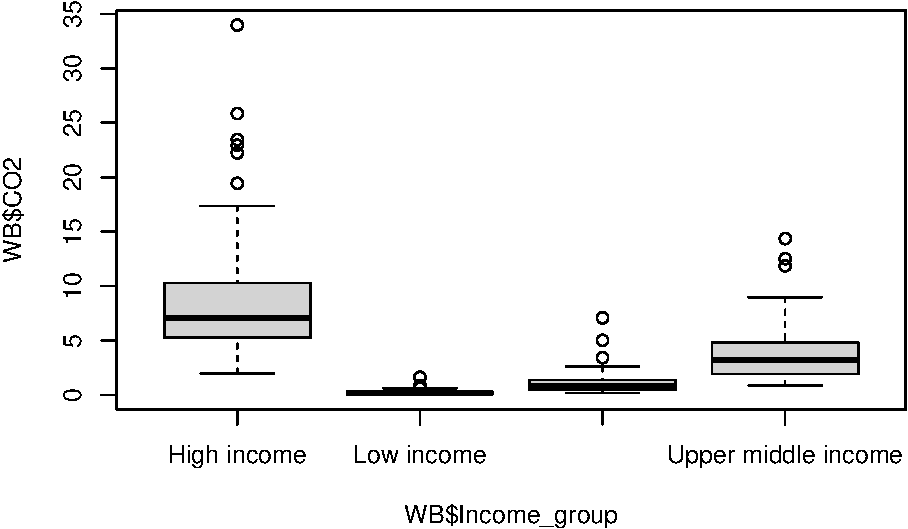
\includegraphics{3rd_Edition_files/figure-latex/unnamed-chunk-247-1.pdf}
\caption{\label{fig:unnamed-chunk-247}CO\textsubscript{2} production per capita by income group}
\end{figure}

This gives us a boxplot showing the CO\textsubscript{2} production per capita of each country in our dataset by income group. The overall pattern is hardly a surprise\ldots{} nonetheless we could make the graph a bit clearer. It need some axis labels, and it would be nice to have our factor levels in a more sensible order. Maybe we might want to shade the boxes as well.

\begin{Shaded}
\begin{Highlighting}[]
\NormalTok{WB}\OperatorTok{$}\NormalTok{Income_group <-}\StringTok{ }\KeywordTok{factor}\NormalTok{(}
\NormalTok{  WB}\OperatorTok{$}\NormalTok{Income_group,}
  \DataTypeTok{levels =} \KeywordTok{c}\NormalTok{(}
    \StringTok{"Low income"}\NormalTok{,}
    \StringTok{"Lower middle income"}\NormalTok{,}
    \StringTok{"Upper middle income"}\NormalTok{,}
    \StringTok{"High income"}
\NormalTok{  )}
\NormalTok{)}

\KeywordTok{boxplot}\NormalTok{(}
\NormalTok{  WB}\OperatorTok{$}\NormalTok{CO2 }\OperatorTok{~}\StringTok{ }\NormalTok{WB}\OperatorTok{$}\NormalTok{Income_group,}
  \DataTypeTok{xlab =} \StringTok{"Income group"}\NormalTok{,}
  \DataTypeTok{ylab =} \KeywordTok{expression}\NormalTok{(}\KeywordTok{paste}\NormalTok{(CO[}\DecValTok{2}\NormalTok{], }\StringTok{" production per capita (tonnes)"}\NormalTok{)),}
  \DataTypeTok{col =} \StringTok{"grey70"}\NormalTok{,}
  \DataTypeTok{cex.axis =} \FloatTok{0.8}
\NormalTok{)}
\end{Highlighting}
\end{Shaded}

\begin{figure}
\centering
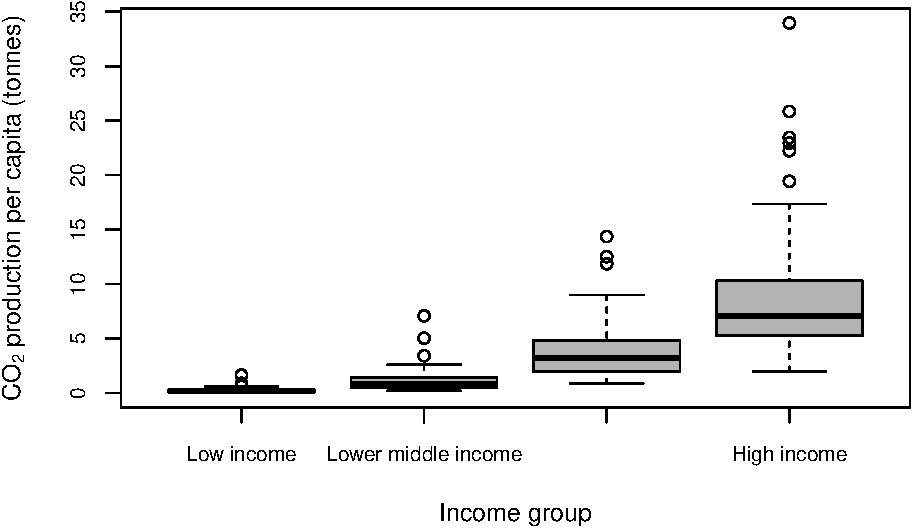
\includegraphics{3rd_Edition_files/figure-latex/unnamed-chunk-248-1.pdf}
\caption{\label{fig:unnamed-chunk-248}Boxplot showing CO\textsubscript{2} production per capita by income group with income group ordered from low to high}
\end{figure}

\texttt{boxplot()} will also plot graphs with more complex combinations of factors. Let's say that we want to look at the way that income relates to CO\textsubscript{2} production, but we'd like to divide our data up by region to see if the effect of income varies goegraphically. A plot with four income levels for each of the seven regions would be prohibitively complex, but we could divide income simply into ``high'' and ``low''.

\begin{Shaded}
\begin{Highlighting}[]
\NormalTok{Income <-}\StringTok{ }\KeywordTok{as.factor}\NormalTok{(}\KeywordTok{ifelse}\NormalTok{(WB}\OperatorTok{$}\NormalTok{Income_group }\OperatorTok{==}\StringTok{ "High income"} \OperatorTok{|}\StringTok{ }\NormalTok{WB}\OperatorTok{$}\NormalTok{Income_group }\OperatorTok{==}\StringTok{ "Upper middle income"}\NormalTok{, }\StringTok{"High income"}\NormalTok{, }\StringTok{"Low income"}\NormalTok{))}
\end{Highlighting}
\end{Shaded}

We've already set our \texttt{Income\_group} factor so that the levels are ordered from low to high, so if we convert the factor to a numeric variable then our two lower income groups will have the values 1 and 2 and our higher income groups will have the values 3 and 4. We can then use the \texttt{ifelse()} function to generate a new vector with ``Low income'' if \texttt{Income\_group} gives us a number 1 or 2 and ``High income'' if it is three or four. Finally we're using the \texttt{factor()} function to convert this to a factor. Now we can use this in a \texttt{boxplot()} function call to draw a plot of CO\textsubscript{2} output conditioned on region and on income.

\begin{Shaded}
\begin{Highlighting}[]
\KeywordTok{boxplot}\NormalTok{(WB}\OperatorTok{$}\NormalTok{CO2 }\OperatorTok{~}\StringTok{ }\NormalTok{Income }\OperatorTok{*}\StringTok{ }\NormalTok{WB}\OperatorTok{$}\NormalTok{Region, }\DataTypeTok{col =} \StringTok{"grey70"}\NormalTok{)}
\end{Highlighting}
\end{Shaded}

\begin{figure}
\centering
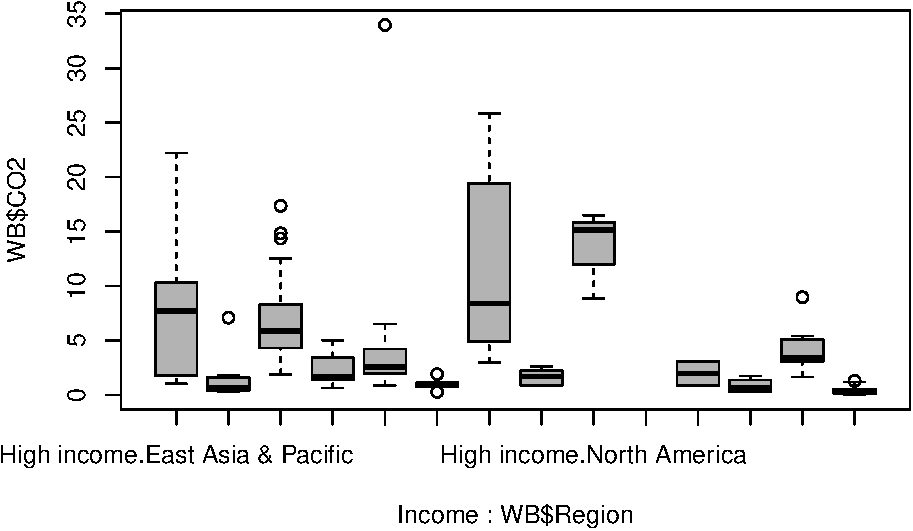
\includegraphics{3rd_Edition_files/figure-latex/unnamed-chunk-250-1.pdf}
\caption{\label{fig:unnamed-chunk-250}Boxplot of national carbon dioxide production per capita by region and income group}
\end{figure}

Hmmm. It's worked but it's not a useable plot at the moment. The x-axis labels are a mess and it's impossible to work out which regions and incomes are represented by what. The plot is also a bit hard to read because the skewed nature of the data means that a lot of our boxes and whiskers are squished down along the x-axis.

Let's remedy the easier things by log\textsubscript{10} transforming the data and by colour coding our boxes depending on income. We can also switch the axis labelling to vertical by setting the parameter \texttt{las\ =\ 2} which might make things a little easier.

\begin{Shaded}
\begin{Highlighting}[]

\NormalTok{palette1 <-}\StringTok{ }\KeywordTok{c}\NormalTok{(}\StringTok{"cadetblue4"}\NormalTok{, }\StringTok{"orange"}\NormalTok{)}

\KeywordTok{boxplot}\NormalTok{(}\KeywordTok{log10}\NormalTok{(WB}\OperatorTok{$}\NormalTok{CO2) }\OperatorTok{~}\StringTok{ }\NormalTok{Income }\OperatorTok{*}\StringTok{ }\NormalTok{WB}\OperatorTok{$}\NormalTok{Region,  }
        \DataTypeTok{col =}\NormalTok{ palette1, }
        \DataTypeTok{las =} \DecValTok{2}\NormalTok{)}
\end{Highlighting}
\end{Shaded}

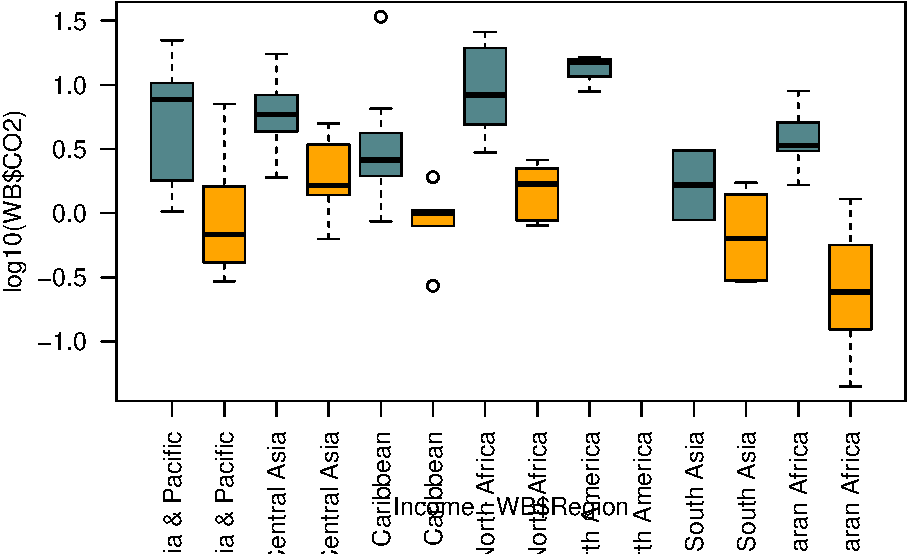
\includegraphics{3rd_Edition_files/figure-latex/unnamed-chunk-251-1.pdf}

Well, some of that worked and some didn't. We've got our log transformation and our colour coding, but the axis is still a disaster and we also need a legend to tell the reader what the colours mean.

\begin{Shaded}
\begin{Highlighting}[]
\KeywordTok{par}\NormalTok{(}\DataTypeTok{mar =} \KeywordTok{c}\NormalTok{(}\FloatTok{9.5}\NormalTok{,}\DecValTok{5}\NormalTok{,}\DecValTok{2}\NormalTok{,}\DecValTok{6}\NormalTok{))}

\KeywordTok{boxplot}\NormalTok{(}\KeywordTok{log10}\NormalTok{(WB}\OperatorTok{$}\NormalTok{CO2) }\OperatorTok{~}\StringTok{ }\NormalTok{Income }\OperatorTok{*}\StringTok{ }\NormalTok{WB}\OperatorTok{$}\NormalTok{Region,  }
        \DataTypeTok{col =}\NormalTok{ palette1, }
        \DataTypeTok{xaxt =} \StringTok{"n"}\NormalTok{,}
        \DataTypeTok{xlab =} \StringTok{""}\NormalTok{,}
        \DataTypeTok{ylab =} \KeywordTok{expression}\NormalTok{(}\KeywordTok{paste}\NormalTok{(Log[}\DecValTok{10}\NormalTok{] , CO[}\DecValTok{2}\NormalTok{], }\StringTok{" Production (tonnes)"}\NormalTok{, }\DataTypeTok{sep =} \StringTok{" "}\NormalTok{)))}

\KeywordTok{axis}\NormalTok{(}\DataTypeTok{side =} \DecValTok{1}\NormalTok{,}
     \DataTypeTok{at =} \KeywordTok{seq}\NormalTok{(}\FloatTok{1.5}\NormalTok{, }\FloatTok{13.5}\NormalTok{, }\DataTypeTok{by =} \DecValTok{2}\NormalTok{),}
     \DataTypeTok{labels =} \KeywordTok{levels}\NormalTok{(WB}\OperatorTok{$}\NormalTok{Region),}
     \DataTypeTok{las =} \DecValTok{2}\NormalTok{,}
     \DataTypeTok{cex.axis =} \FloatTok{0.8}\NormalTok{)}

\KeywordTok{par}\NormalTok{(}\DataTypeTok{xpd =} \OtherTok{TRUE}\NormalTok{)}

\KeywordTok{legend}\NormalTok{(}\DataTypeTok{x =} \DecValTok{15}\NormalTok{, }\DataTypeTok{y =} \FloatTok{1.5}\NormalTok{,}
       \DataTypeTok{legend =} \KeywordTok{c}\NormalTok{(}\StringTok{"High"}\NormalTok{, }\StringTok{"Low"}\NormalTok{),}
       \DataTypeTok{fill =}\NormalTok{ palette1,}
       \DataTypeTok{bty =} \StringTok{"n"}\NormalTok{,}
       \DataTypeTok{title =} \StringTok{"Income"}\NormalTok{)}
\end{Highlighting}
\end{Shaded}

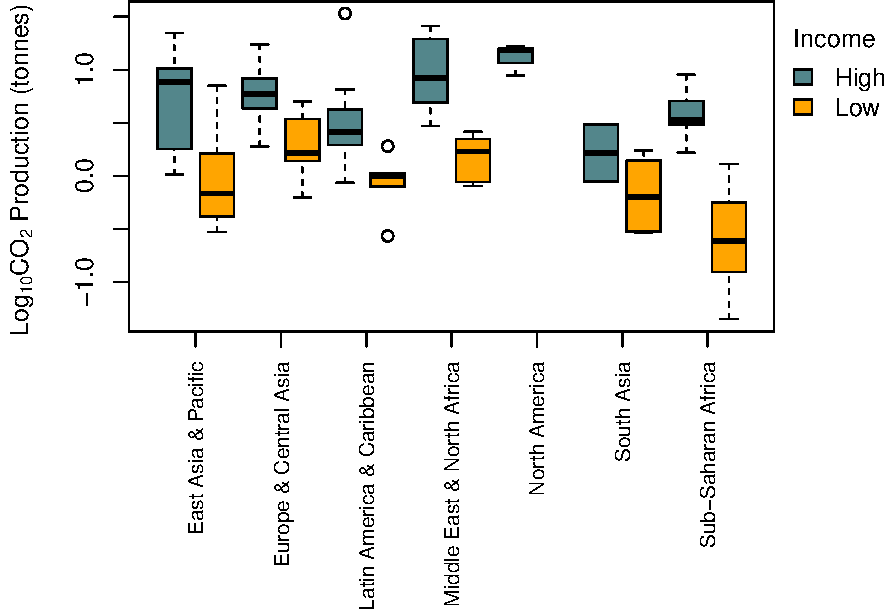
\includegraphics{3rd_Edition_files/figure-latex/unnamed-chunk-252-1.pdf}

\hypertarget{bar-charts}{%
\section{Bar charts}\label{bar-charts}}

The bar chart is one of the most common types of graphic that you'll see used to show patterns in data. As with boxplots, R has a specific function for drawing these: \texttt{barplot()}. The output is perhaps a little eccentric but it can easily be made more conventional. Here's an example using the data on CO\textsubscript{2} production by income group that we saw when we were looking at boxplots. We want to plot the mean CO\textsubscript{2} production per capita for each group so we need to calculate this before we do anything else. We'll use the \texttt{tapply()} function to do this.

\begin{Shaded}
\begin{Highlighting}[]
\NormalTok{CO2_means <-}\StringTok{ }\KeywordTok{tapply}\NormalTok{(WB}\OperatorTok{$}\NormalTok{CO2, WB}\OperatorTok{$}\NormalTok{Income_group, mean)}

\NormalTok{CO2_means}
\NormalTok{         Low income Lower middle income Upper middle income         High income }
            \FloatTok{0.31712}             \FloatTok{1.21814}             \FloatTok{4.05665}             \FloatTok{9.46772} 
\end{Highlighting}
\end{Shaded}

Let's see what we get if we just feed this to \texttt{barplot()}.

\begin{Shaded}
\begin{Highlighting}[]
\KeywordTok{barplot}\NormalTok{(CO2_means)}
\end{Highlighting}
\end{Shaded}

\begin{figure}
\centering
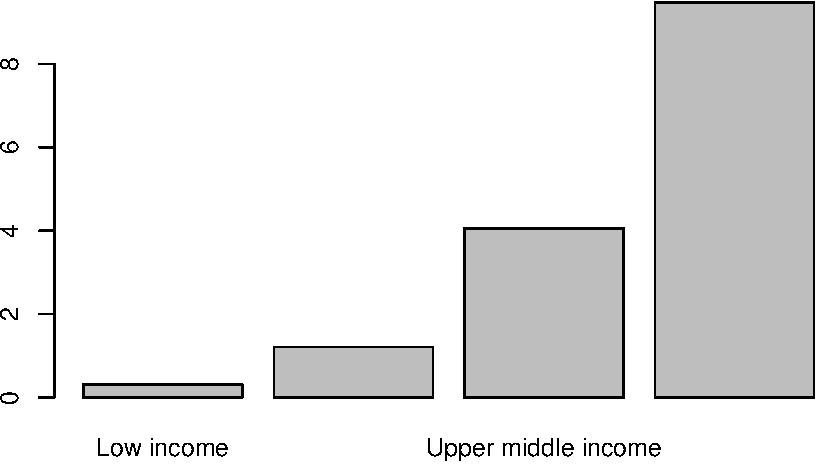
\includegraphics{3rd_Edition_files/figure-latex/unnamed-chunk-254-1.pdf}
\caption{\label{fig:unnamed-chunk-254}Barplot of mean carbon dioxide production per capita by income group}
\end{figure}

Overall it's not bad but could obviously be better, especially with regards to the x-axis labels. We can fix the x-axis labels by making them smaller and losing the word ``income'' from each to make them more concise.

\begin{Shaded}
\begin{Highlighting}[]

\KeywordTok{names}\NormalTok{(CO2_means) <-}\StringTok{ }\KeywordTok{c}\NormalTok{(}\StringTok{"Low"}\NormalTok{, }\StringTok{"Lower middle"}\NormalTok{, }\StringTok{"Upper middle"}\NormalTok{, }\StringTok{"High"}\NormalTok{)}

\KeywordTok{barplot}\NormalTok{(CO2_means,}
        \DataTypeTok{cex.axis =} \FloatTok{0.7}\NormalTok{,}
        \DataTypeTok{cex.lab =} \FloatTok{0.9}\NormalTok{,}
        \DataTypeTok{cex.names =} \FloatTok{0.7}\NormalTok{,}
        \DataTypeTok{xlab =} \StringTok{"Income group"}\NormalTok{,}
        \DataTypeTok{ylab =} \KeywordTok{expression}\NormalTok{(}\KeywordTok{paste}\NormalTok{(Log[}\DecValTok{10}\NormalTok{] , CO[}\DecValTok{2}\NormalTok{], }\StringTok{" Production (tonnes)"}\NormalTok{, }\DataTypeTok{sep =} \StringTok{" "}\NormalTok{)))}
\end{Highlighting}
\end{Shaded}

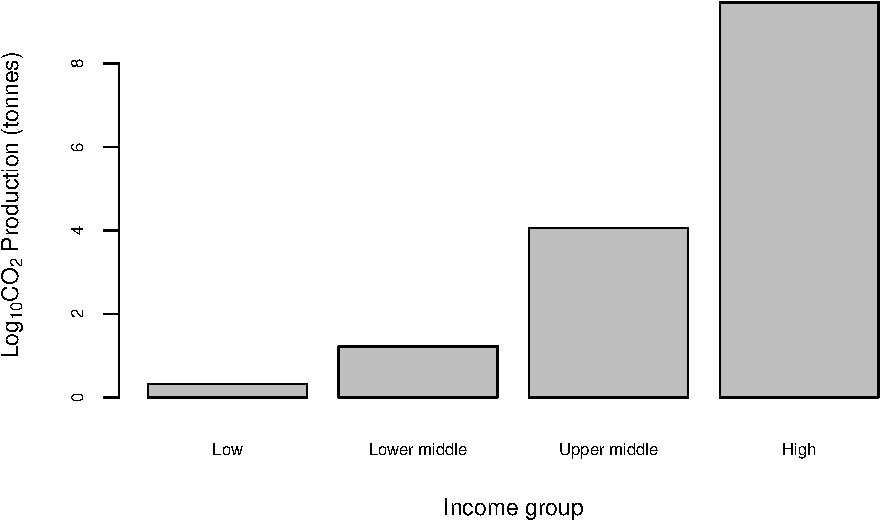
\includegraphics{3rd_Edition_files/figure-latex/unnamed-chunk-255-1.pdf}

Not bad. Let's run through that code and see what it all does.

\texttt{names(CO2\_means)\ \textless{}-\ c("Low",\ "Lower\ middle",\ "Upper\ middle",\ "High")}

Changes then names for each entry in the \texttt{CO2\_means} object. \texttt{barplot()} uses these names for the x-axis names so this changes them in the plot as well.

\texttt{barplot(CO2\_means,}

Tells \texttt{barplot()} where to find the data.

\begin{verbatim}
   `cex.axis = 0.7,
    cex.lab = 0.9,
    cex.names = 0.7,`
    
\end{verbatim}

Adjusts the sizes of the numbers on the y-axis (\texttt{cex.axis}), the axis labels (\texttt{cex.lab}) and the names on the x-axis (\texttt{cex.names}). Recall that \texttt{cex} is short for \textbf{C}haracter \textbf{EX}pansion so a value of 1 is keep the default size, 0.5 is plot at half the default size and 2 is twice the default size.

\begin{verbatim}
   `xlab = "Income group",
    ylab = expression(paste(Log[10] , CO[2], " Production (tonnes)", sep = " ")))`
    
\end{verbatim}

These two arguments specifiy the text for the axis labels and as before we're using a somewhat complex \texttt{expression()} function call to give us a proper subscript in CO\textsubscript{2}.

One thing that might be causing concern here is the lack of a ``proper'' x-axis with a line and tickmarks. If you need one you can add one using \texttt{axis()}.

\begin{Shaded}
\begin{Highlighting}[]

\KeywordTok{barplot}\NormalTok{(CO2_means,}
        \DataTypeTok{cex.axis =} \FloatTok{0.7}\NormalTok{,}
        \DataTypeTok{cex.lab =} \FloatTok{0.9}\NormalTok{,}
        \DataTypeTok{cex.names =} \FloatTok{0.7}\NormalTok{,}
        \DataTypeTok{xlab =} \StringTok{"Income group"}\NormalTok{,}
        \DataTypeTok{ylab =} \KeywordTok{expression}\NormalTok{(}\KeywordTok{paste}\NormalTok{(}\StringTok{"Mean "}\NormalTok{, CO[}\DecValTok{2}\NormalTok{], }\StringTok{" Production (tonnes)"}\NormalTok{, }\DataTypeTok{sep =} \StringTok{" "}\NormalTok{)))}

\NormalTok{ticks <-}\StringTok{ }\KeywordTok{barplot}\NormalTok{(CO2_means, }\DataTypeTok{plot =} \OtherTok{FALSE}\NormalTok{)}

\KeywordTok{axis}\NormalTok{(}\DataTypeTok{side =} \DecValTok{1}\NormalTok{, }\DataTypeTok{at =}\NormalTok{ ticks, }\DataTypeTok{labels =} \OtherTok{FALSE}\NormalTok{)}
\end{Highlighting}
\end{Shaded}

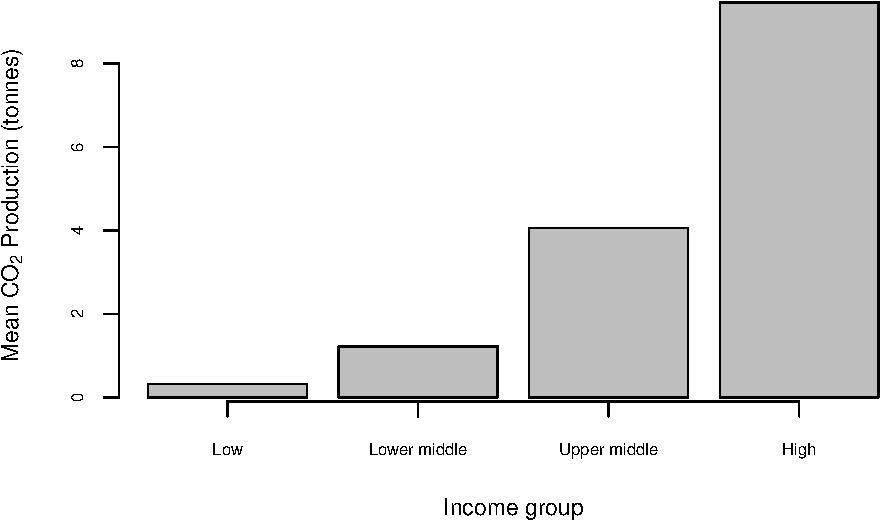
\includegraphics{3rd_Edition_files/figure-latex/unnamed-chunk-256-1.pdf}

Here \texttt{axis(side\ =\ 1,\ at\ =\ ticks,\ labels\ =\ FALSE)} draws in an axis on the x-axis only (\texttt{side\ =\ 1}) with no labels etc. The trick with drawing an axis for a bar plot is that the location of the centres of the bars is not obvious: it's not 1,2,3 \& 4 as you might expect. To extract the locations we've used

\texttt{ticks\ \textless{}-\ barplot(CO2\_means,\ plot\ =\ FALSE)}

which takes advantage of the fact that if you save the output of a \texttt{barplot()} call to an object what it saves is in fact the locations of the bar centres and nothing else (of course). The \texttt{plot\ =\ FALSE} argument stops it drawing the barplot in your graphics window unnecessarily.

\hypertarget{more-complex-barplots}{%
\subsection{More complex barplots}\label{more-complex-barplots}}

Lots of people like making complicated bar charts with groups of different means displayed together. If you're one of these people (I am not) you will want to know how to do this in R. Let's generate a more complicated set of means using the ``income'' factor which we used when making boxplots, so we'll have a mean CO\textsubscript{2} production figure for high and low income countries in each of our regions.

\begin{Shaded}
\begin{Highlighting}[]
\NormalTok{income <-}\StringTok{ }\KeywordTok{factor}\NormalTok{(}\KeywordTok{ifelse}\NormalTok{(}\KeywordTok{as.numeric}\NormalTok{(WB}\OperatorTok{$}\NormalTok{Income_group) }\OperatorTok{<}\DecValTok{3}\NormalTok{, }\StringTok{"Low income"}\NormalTok{, }\StringTok{"High income"}\NormalTok{))}

\NormalTok{CO2_means2 <-}\StringTok{ }\KeywordTok{tapply}\NormalTok{(WB}\OperatorTok{$}\NormalTok{CO2, }\DataTypeTok{INDEX =} \KeywordTok{list}\NormalTok{(income, WB}\OperatorTok{$}\NormalTok{Region), mean)}

\NormalTok{CO2_means2}
\NormalTok{            East Asia }\OperatorTok{&}\StringTok{ }\NormalTok{Pacific Europe }\OperatorTok{&}\StringTok{ }\NormalTok{Central Asia Latin America }\OperatorTok{&}\StringTok{ }\NormalTok{Caribbean}
\NormalTok{High income              }\FloatTok{7.8760}                \FloatTok{6.6059}                    \FloatTok{4.1153}
\NormalTok{Low income               }\FloatTok{1.3309}                \FloatTok{2.4207}                    \FloatTok{1.0050}
\NormalTok{            Middle East }\OperatorTok{&}\StringTok{ }\NormalTok{North Africa North America South Asia}
\NormalTok{High income                    }\FloatTok{11.7631}          \FloatTok{13.5}    \FloatTok{1.97681}
\NormalTok{Low income                      }\FloatTok{1.6521}            \OtherTok{NA}    \FloatTok{0.83957}
\NormalTok{            Sub}\OperatorTok{-}\NormalTok{Saharan Africa}
\NormalTok{High income            }\FloatTok{4.32719}
\NormalTok{Low income             }\FloatTok{0.37091}
\end{Highlighting}
\end{Shaded}

There is one missing value, this is because there are no ``Low income'' nations in the North America region. What we want is a bar chart with two bars side by side for each region. Let's see what \texttt{barplot()} makes of our matrix.

\begin{Shaded}
\begin{Highlighting}[]
\KeywordTok{barplot}\NormalTok{(CO2_means2, }
        \DataTypeTok{beside =} \OtherTok{TRUE}\NormalTok{,}
        \DataTypeTok{legend =} \OtherTok{TRUE}\NormalTok{)}
\end{Highlighting}
\end{Shaded}

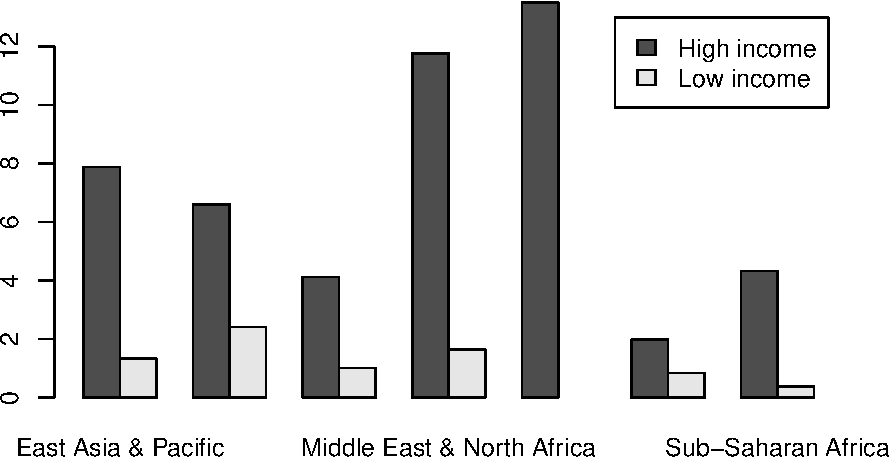
\includegraphics{3rd_Edition_files/figure-latex/unnamed-chunk-258-1.pdf}

Two things to look at in the code are the extra arguments I've added to the \texttt{barplot()} function call. \texttt{beside\ =\ TRUE} means that the bars are plotted next to each other: the alternative with \texttt{beside\ =\ FALSE} is a stacked bar chart, which (in my opinion at least) is rarely useful. Secondly we have \texttt{legend\ =\ TRUE}. \texttt{barplot()} is one of the few (maybe the only?) plotting functions in Base R which will automatically generate a legend for you. YOu can see this in the top right of our figure.

Note that if the grouping is not what you want (in this case if the bars were grouped by income not region) you can switch them by using the \texttt{t()} function which will transpose our matrix, or in other words flip it on its side. This is because \texttt{barplot()} uses the columns in a matrix of data for grouping, so \texttt{barplot(t(CO2\_means2),\ ...} would give the other grouping.

OK, let's finish up by making this a publication-quality chart. We need to deal with the labels for the x-axis as we did when we plotted a similar chart using \texttt{boxplot()}, by rotating the x-axis labels and enlarging the lower margin. We're going to shrink the text size and add an axis, and we're going use the same colour scheme that we used for our boxplot.

\begin{Shaded}
\begin{Highlighting}[]
\CommentTok{#Set up colour palette}
\NormalTok{palette1 <-}\StringTok{ }\KeywordTok{c}\NormalTok{(}\StringTok{"cadetblue4"}\NormalTok{, }\StringTok{"orange"}\NormalTok{) }

\CommentTok{#Alter the margins}
\KeywordTok{par}\NormalTok{(}\DataTypeTok{mar =} \KeywordTok{c}\NormalTok{(}\FloatTok{9.5}\NormalTok{,}\DecValTok{5}\NormalTok{,}\DecValTok{2}\NormalTok{,}\DecValTok{6}\NormalTok{))}

\CommentTok{#Find where the ticks should be for the x-axis}
\NormalTok{ticks <-}\StringTok{ }\KeywordTok{barplot}\NormalTok{(CO2_means2, }\DataTypeTok{beside =} \OtherTok{TRUE}\NormalTok{, }\DataTypeTok{plot =} \OtherTok{FALSE}\NormalTok{)}
\NormalTok{ticks <-}\StringTok{ }\KeywordTok{colMeans}\NormalTok{(ticks)}

\CommentTok{#Draw the graph}
\KeywordTok{barplot}\NormalTok{(CO2_means2, }
        \DataTypeTok{beside =} \OtherTok{TRUE}\NormalTok{,}
        \DataTypeTok{legend =} \OtherTok{TRUE}\NormalTok{,}
        \DataTypeTok{col =}\NormalTok{ palette1,}
        \DataTypeTok{las =} \DecValTok{2}\NormalTok{,}
        \DataTypeTok{cex.axis =} \FloatTok{0.8}\NormalTok{,}
        \DataTypeTok{cex.names =} \FloatTok{0.8}\NormalTok{,}
        \DataTypeTok{cex.lab =} \FloatTok{0.9}\NormalTok{,}
        \DataTypeTok{ylab =} \KeywordTok{expression}\NormalTok{(}\KeywordTok{paste}\NormalTok{(}\StringTok{"Mean "}\NormalTok{, CO[}\DecValTok{2}\NormalTok{], }\StringTok{" Production (tonnes)"}\NormalTok{, }\DataTypeTok{sep =} \StringTok{" "}\NormalTok{)))}

\CommentTok{#Add the axis}
\KeywordTok{axis}\NormalTok{(}\DataTypeTok{side =} \DecValTok{1}\NormalTok{, }\DataTypeTok{at =}\NormalTok{ ticks, }\DataTypeTok{labels =} \OtherTok{FALSE}\NormalTok{)}
\end{Highlighting}
\end{Shaded}

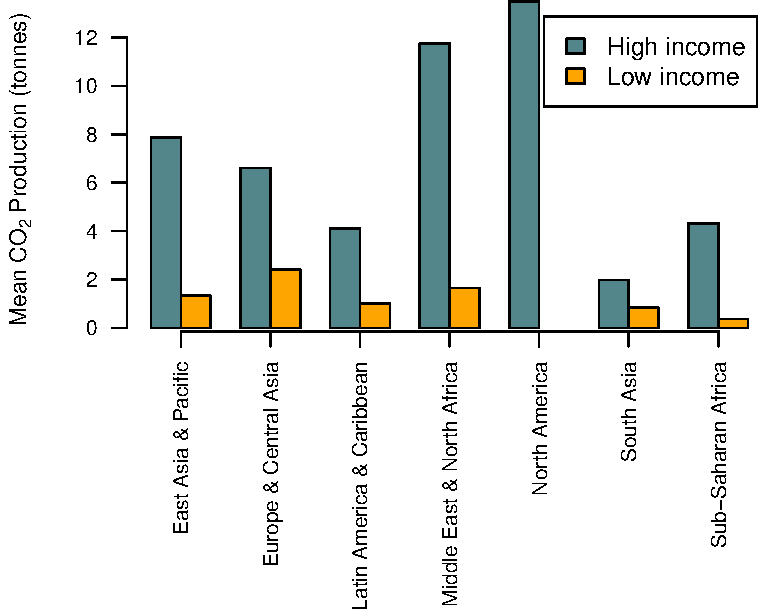
\includegraphics{3rd_Edition_files/figure-latex/unnamed-chunk-259-1.pdf}

All should be relatively clear, but you might be wondering about this:

\begin{Shaded}
\begin{Highlighting}[]
\CommentTok{#Find where the ticks should be for the x-axis  }
\NormalTok{ticks <-}\StringTok{ }\KeywordTok{barplot}\NormalTok{(CO2_means2, }\DataTypeTok{beside =} \OtherTok{TRUE}\NormalTok{, }\DataTypeTok{plot =} \OtherTok{FALSE}\NormalTok{)  }
\NormalTok{ticks <-}\StringTok{ }\KeywordTok{colMeans}\NormalTok{(ticks)}
\end{Highlighting}
\end{Shaded}

Why use \texttt{colMeans()} here? The answer is that the first line \texttt{ticks\ \textless{}-\ barplot(CO2\_means2,\ beside\ =\ TRUE,\ plot\ =\ FALSE)} will return a matrix with the location of each bar. We want the middle of each group of bars, and since each group is a coloumn we can just take the mean value of each column to get that middle point. This point will come up again when we add some error bars to this graph in the next chapter.

\hypertarget{other-types-of-plot}{%
\section{Other types of plot}\label{other-types-of-plot}}

In addition to \texttt{plot()}, there are lots of other functions for drawing graphs, and you can produce just about any sort of plot you can imagine using R. We've already seen \texttt{barplot()} in action, here are some further examples.

\hypertarget{histogram-with-overlaid-probability-density-estimate}{%
\subsection{Histogram with overlaid probability density estimate}\label{histogram-with-overlaid-probability-density-estimate}}

We've already seen that is an argument for the \texttt{hist()} function called ``\texttt{freq}'' which is normally set to \texttt{NULL}, but if set to \texttt{FALSE} will draw a frequency histogram with the y axis scaled not to count but to the relative frequency density, such that the total area under the graph=1. A probability density estimate can then be obtained using \texttt{density()}, which computes a kernel density estimate for the variable in question. Here is a frequency histogram for the data on forest cover from our World Bank dataset with a density estimate overlaid.

\begin{Shaded}
\begin{Highlighting}[]

\KeywordTok{hist}\NormalTok{(WB}\OperatorTok{$}\NormalTok{Forest_area,}
     \DataTypeTok{breaks=}\DecValTok{15}\NormalTok{, }
     \DataTypeTok{col=}\StringTok{"Cadetblue4"}\NormalTok{, }
     \DataTypeTok{ylab=}\StringTok{"Relative frequency"}\NormalTok{,}
     \DataTypeTok{xlab =} \StringTok{"Forest area (percentage of total)"}\NormalTok{,}
     \DataTypeTok{freq=}\NormalTok{F)}

\KeywordTok{lines}\NormalTok{(}\KeywordTok{density}\NormalTok{(WB}\OperatorTok{$}\NormalTok{Forest_area, }\DataTypeTok{na.rm =} \OtherTok{TRUE}\NormalTok{))}
\end{Highlighting}
\end{Shaded}

\begin{figure}
\centering
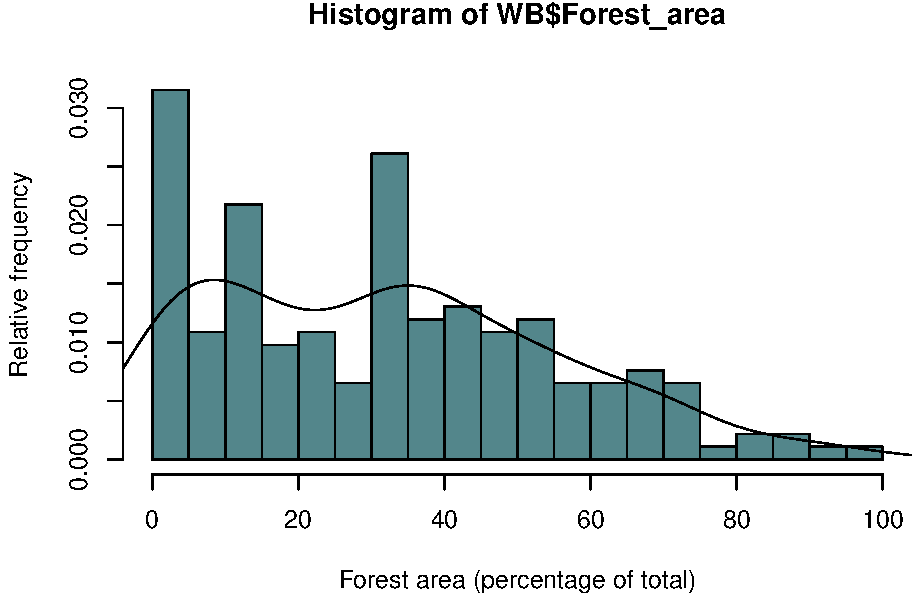
\includegraphics{3rd_Edition_files/figure-latex/unnamed-chunk-261-1.pdf}
\caption{\label{fig:unnamed-chunk-261}Frequency histogram of forest cover by country with probability density estimate drawn as a line.}
\end{figure}

We can increase or decrease the amount of smoothing in the density estimate by using the ``adjust'' argument.

\begin{Shaded}
\begin{Highlighting}[]

\KeywordTok{hist}\NormalTok{(WB}\OperatorTok{$}\NormalTok{Forest_area,}
     \DataTypeTok{breaks=}\DecValTok{15}\NormalTok{, }
     \DataTypeTok{col=}\StringTok{"Cadetblue4"}\NormalTok{, }
     \DataTypeTok{ylab=}\StringTok{"Relative frequency"}\NormalTok{,}
     \DataTypeTok{xlab =} \StringTok{"Forest area (percentage of total)"}\NormalTok{,}
     \DataTypeTok{freq=}\NormalTok{F)}

\CommentTok{#Less smoothing}
\KeywordTok{lines}\NormalTok{(}\KeywordTok{density}\NormalTok{(WB}\OperatorTok{$}\NormalTok{Forest_area, }\DataTypeTok{na.rm =} \OtherTok{TRUE}\NormalTok{, }\DataTypeTok{adjust =} \FloatTok{0.5}\NormalTok{), }
      \DataTypeTok{lty =} \DecValTok{2}\NormalTok{, }
      \DataTypeTok{lwd =} \DecValTok{2}\NormalTok{)}

\CommentTok{#More smoothing}
\KeywordTok{lines}\NormalTok{(}\KeywordTok{density}\NormalTok{(WB}\OperatorTok{$}\NormalTok{Forest_area, }\DataTypeTok{na.rm =} \OtherTok{TRUE}\NormalTok{, }\DataTypeTok{adjust =} \FloatTok{0.2}\NormalTok{), }
      \DataTypeTok{lty =} \DecValTok{3}\NormalTok{, }
      \DataTypeTok{lwd =} \DecValTok{2}\NormalTok{)}
\end{Highlighting}
\end{Shaded}

\begin{figure}
\centering
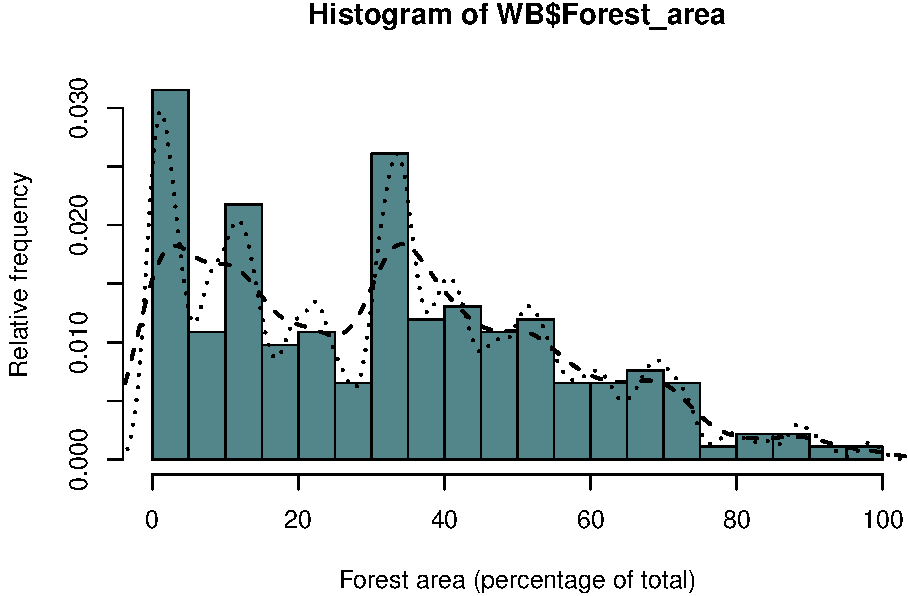
\includegraphics{3rd_Edition_files/figure-latex/unnamed-chunk-262-1.pdf}
\caption{\label{fig:unnamed-chunk-262}As the previous figure but with two probability density estimates showing different amounts of smoothing}
\end{figure}

Here I've plotted two kernel density estimates. The first one has the amount of smoothing reduced from the default by half (\texttt{adjust=0.5}), giving a line that closely follows the distribution of the data, and the second has the amount of smoothing set to twice the default (\texttt{adjust=2}), giving a much smoother line. Two further points to note are firstly that I set the type of line using the \texttt{lty=} parameter and increased the line width using \texttt{lwd\ =\ 2}, and secondly the location of the various arguments. Because the \texttt{adjust=} argument is used in the \texttt{density()} function it's kept within the brackets associated with the function, whereas the \texttt{lty=} and \texttt{lwd=} arguments go with the \texttt{lines()} function so it's inside the outer set of brackets. Easy to get confused if you don't think about which arguments are associated with which functions.

\hypertarget{pie-graph}{%
\subsection{Pie graph}\label{pie-graph}}

Before you draw a pie graph, please read the help file for the \texttt{pie()} function, in particular the part beginning ``Pie charts are a very bad way of displaying information\ldots{}''. If you still want to draw a pie graph, please go directly to your nearest decent library and read the whole of Edward Tufte's brilliant and beautiful book, \emph{The Visual Display of Quantitative Information} (published by Graphics Press USA, 2nd edition 2001, ISBN 978-0961392147). That should teach you the error of your ways. If, however, you still want to draw a pie graph for some reason (perhaps you're a journalist or a politician and want to disguise the patterns in some data) the you can use the \texttt{pie()} function. Here's an example with made up data:

\begin{Shaded}
\begin{Highlighting}[]
\NormalTok{chart.numbers<-}\KeywordTok{c}\NormalTok{(}\DecValTok{15}\NormalTok{,}\DecValTok{108}\NormalTok{,}\DecValTok{220}\NormalTok{,}\DecValTok{22}\NormalTok{,}\DecValTok{170}\NormalTok{)}
\KeywordTok{names}\NormalTok{(chart.numbers)<-}\KeywordTok{c}\NormalTok{(}\StringTok{"Bar"}\NormalTok{, }\StringTok{"2D Pie"}\NormalTok{, }\StringTok{"3D Pie"}\NormalTok{, }\StringTok{"Scatter"}\NormalTok{, }\StringTok{"Doughnut"}\NormalTok{)}
\NormalTok{chart.numbers2<-}\KeywordTok{c}\NormalTok{(}\DecValTok{119}\NormalTok{,}\DecValTok{12}\NormalTok{,}\DecValTok{280}\NormalTok{,}\DecValTok{5}\NormalTok{)}
\KeywordTok{names}\NormalTok{(chart.numbers2)<-}\KeywordTok{c}\NormalTok{(}\StringTok{"Bar"}\NormalTok{, }\StringTok{"2D Pie"}\NormalTok{, }\StringTok{"Scatter"}\NormalTok{, }\StringTok{"Doughnut"}\NormalTok{)}
\KeywordTok{par}\NormalTok{(}\DataTypeTok{mfrow=}\KeywordTok{c}\NormalTok{(}\DecValTok{1}\NormalTok{,}\DecValTok{2}\NormalTok{))}
\KeywordTok{pie}\NormalTok{(chart.numbers)}
\KeywordTok{text}\NormalTok{(}\DecValTok{0}\NormalTok{,}\DecValTok{1}\NormalTok{, }\StringTok{"Frequencies of graphs in marketing material"}\NormalTok{, }\DataTypeTok{cex=}\FloatTok{0.6}\NormalTok{, }\DataTypeTok{font=}\DecValTok{2}\NormalTok{)}
\KeywordTok{pie}\NormalTok{(chart.numbers2)}
\KeywordTok{text}\NormalTok{(}\DecValTok{0}\NormalTok{,}\DecValTok{1}\NormalTok{, }\StringTok{"Frequencies of graphs in research papers"}\NormalTok{, }\DataTypeTok{cex=}\FloatTok{0.6}\NormalTok{, }\DataTypeTok{font=}\DecValTok{2}\NormalTok{)}
\end{Highlighting}
\end{Shaded}

\begin{figure}
\centering
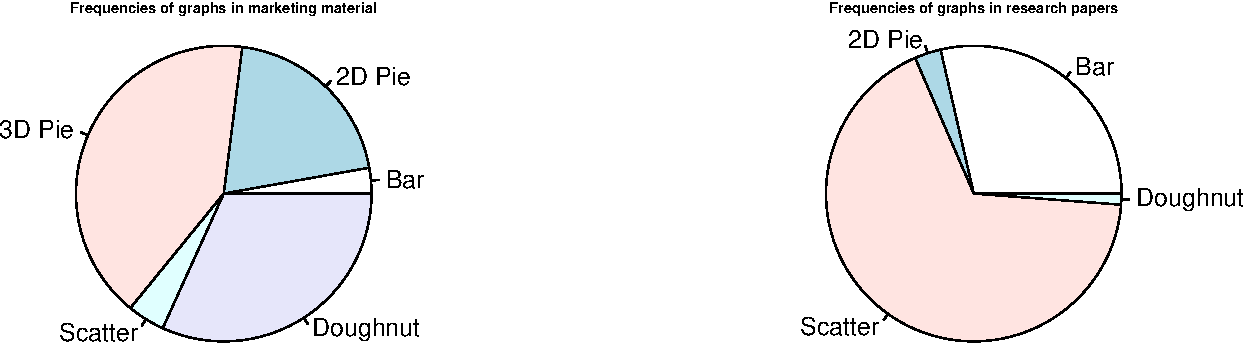
\includegraphics{3rd_Edition_files/figure-latex/graph23-1.pdf}
\caption{\label{fig:graph23}Pie graphs. Nothing more to say.}
\end{figure}

There you are. The default colours are a bit meh but I can't be bothered to fix them.

\hypertarget{d-scatterplot}{%
\subsection{3D scatterplot}\label{d-scatterplot}}

More data visualisations that are filed in the ``best avoided'' drawer. In general it's best to try to avoid presenting your data in ``3D'' graphs if at all possible because there are inevitable distortions that appear when you try to show a 3D cloud of points or surface in 2D, and the patterns in the data can appear very different depending on the angle of view. Nonetheless, there are times when it's hard to find an alternative, and if you can't avoid it there are a number of functions in R to draw 3D graphs. Here we'll use the \texttt{scatterplot3d()} function from the \texttt{scatterplot3d} package. Some other useful 3D plotting functions are in the lattice package, including \texttt{cloud()} which also plots 3D scatterplots and \texttt{wireframe()} which draws a surface.

Some simulated data:

X variable is random and uniformly distributed between 0 and 12

\begin{Shaded}
\begin{Highlighting}[]
\NormalTok{x1<-}\KeywordTok{runif}\NormalTok{(}\DecValTok{25}\NormalTok{, }\DataTypeTok{min=}\DecValTok{0}\NormalTok{, }\DataTypeTok{max=}\DecValTok{12}\NormalTok{)        }
\end{Highlighting}
\end{Shaded}

y variable is random and normally distributed with a mean of 15 and a standard deviation of 3

\begin{Shaded}
\begin{Highlighting}[]
\NormalTok{y1<-}\KeywordTok{rnorm}\NormalTok{(}\DecValTok{25}\NormalTok{, }\DataTypeTok{mean=}\DecValTok{15}\NormalTok{, }\DataTypeTok{sd=}\DecValTok{3}\NormalTok{)    }
\end{Highlighting}
\end{Shaded}

Some randomly distributed error for our z variable

\begin{Shaded}
\begin{Highlighting}[]
\NormalTok{err1<-}\KeywordTok{rnorm}\NormalTok{(}\DecValTok{25}\NormalTok{,}\DecValTok{0}\NormalTok{,}\DecValTok{2}\NormalTok{)         }
\end{Highlighting}
\end{Shaded}

Calculate the z variable

\begin{Shaded}
\begin{Highlighting}[]
\NormalTok{z1<-}\FloatTok{0.8}\OperatorTok{*}\NormalTok{x1}\FloatTok{+1.5}\OperatorTok{*}\NormalTok{y1}\OperatorTok{+}\NormalTok{err1      }
\end{Highlighting}
\end{Shaded}

Plot the graph. Setting type to ``h'' gives us drop lines from each data point.

\begin{Shaded}
\begin{Highlighting}[]
\KeywordTok{scatterplot3d}\NormalTok{(x1, y1, z1, }\DataTypeTok{type=}\StringTok{"h"}\NormalTok{, }\DataTypeTok{pch=}\DecValTok{16}\NormalTok{) }
\end{Highlighting}
\end{Shaded}

\begin{figure}
\centering
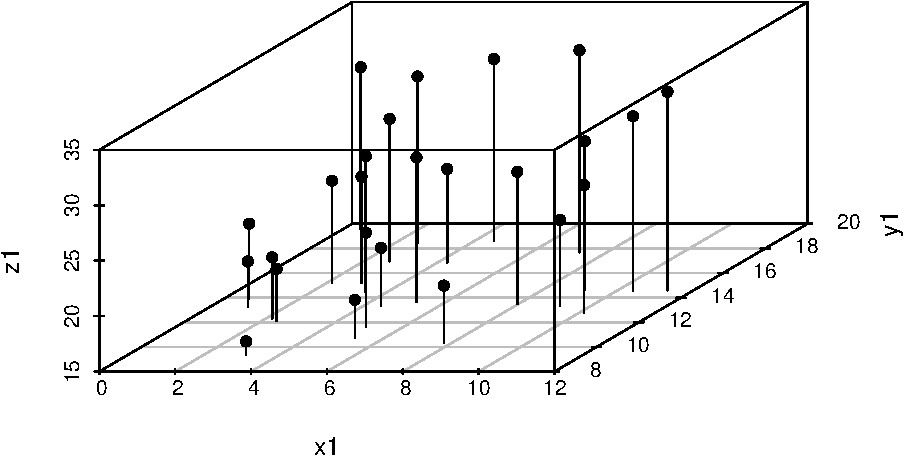
\includegraphics{3rd_Edition_files/figure-latex/graph24-1.pdf}
\caption{\label{fig:graph24}3D scatterplot example}
\end{figure}

\hypertarget{contour-plot}{%
\subsection{Contour plot}\label{contour-plot}}

The earwig \emph{Forficula auricularia} is known to occur in two male morphs, a ``brachylabic'' morph with small forceps and a ``macrolabic'' morph with large forceps which is thought to pursue a more aggressive strategy for competing with rival males and acquiring mates (see Tomkins and Brown 2004, Nature 431 1099-1103 for more details). The graph below is a scatterplot of forceps length (on the y-axis) against pronotum width (a measure of overall body size) on the x-axis for an earwig population on Brownsman Island in the Farne Islands archipelago, the data being kindly supplied to me by Joe Tomkins. We can see some form of structure in this scatterplot, but it might help our visualisation of what's going on if we drew a contour plot showing where the densest groups of points are.

\begin{Shaded}
\begin{Highlighting}[]
\KeywordTok{plot}\NormalTok{(earwig}\OperatorTok{$}\NormalTok{fcp}\OperatorTok{~}\NormalTok{earwig}\OperatorTok{$}\NormalTok{pron,}
     \DataTypeTok{xlab =} \StringTok{"Pronotum width (mm)"}\NormalTok{,}
     \DataTypeTok{ylab =} \StringTok{"Forceps length (mm)"}\NormalTok{)}
\end{Highlighting}
\end{Shaded}

\begin{figure}
\centering
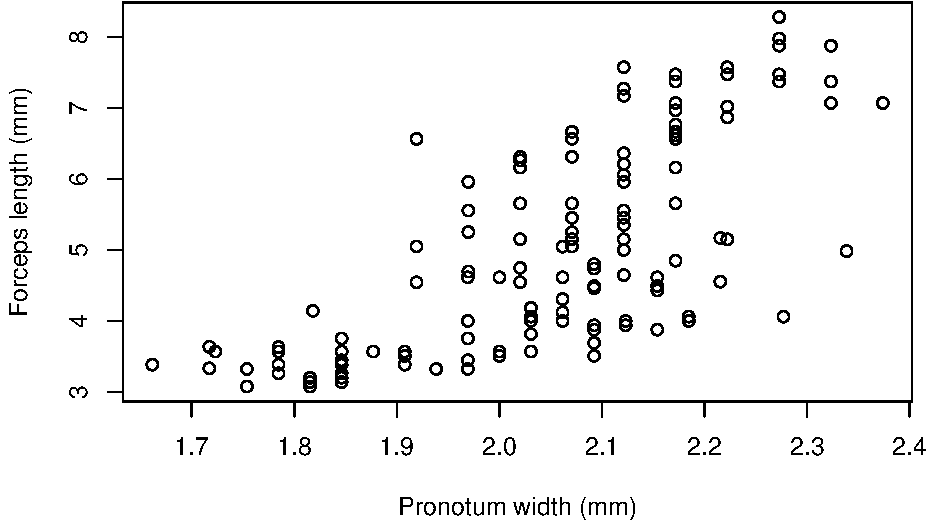
\includegraphics{3rd_Edition_files/figure-latex/unnamed-chunk-268-1.pdf}
\caption{\label{fig:unnamed-chunk-268}Scatterplot of forceps length versus pronotum width for the earwig Forficula airicularia}
\end{figure}

To estimate the density of this 2D dataset we can use the \texttt{kde2d()} function from the MASS package, which fits a 2D kernel density estimator to the data.

\begin{Shaded}
\begin{Highlighting}[]
\KeywordTok{library}\NormalTok{(MASS)}
\NormalTok{earwig.density<-}\KeywordTok{kde2d}\NormalTok{(earwig}\OperatorTok{$}\NormalTok{pron, earwig}\OperatorTok{$}\NormalTok{fcp, }\DataTypeTok{n=}\DecValTok{200}\NormalTok{)}
\end{Highlighting}
\end{Shaded}

Having calculated the density estimator we can then draw a contour plot using the \texttt{contour()} function.

\begin{Shaded}
\begin{Highlighting}[]
\KeywordTok{contour}\NormalTok{(earwig.density, }\DataTypeTok{xlab=}\StringTok{"Pronotum width (mm)"}\NormalTok{, }\DataTypeTok{ylab=}\StringTok{"Forceps length (mm)"}\NormalTok{)}
\end{Highlighting}
\end{Shaded}

\begin{figure}
\centering
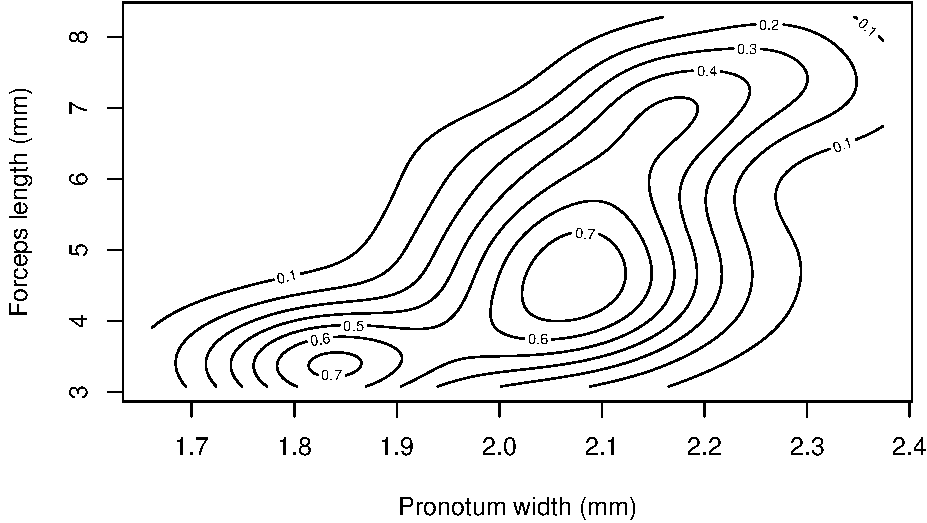
\includegraphics{3rd_Edition_files/figure-latex/unnamed-chunk-270-1.pdf}
\caption{\label{fig:unnamed-chunk-270}Contour plot of earwig forceps length versus pronotum width}
\end{figure}

We can overlay the data points onto the plot using \texttt{points()} ----- more on this in the next chapter.

\begin{Shaded}
\begin{Highlighting}[]
\KeywordTok{points}\NormalTok{(earwig}\OperatorTok{$}\NormalTok{pron, earwig}\OperatorTok{$}\NormalTok{fcp, }\DataTypeTok{pch=}\DecValTok{16}\NormalTok{, }\DataTypeTok{cex=}\FloatTok{0.6}\NormalTok{)}
\end{Highlighting}
\end{Shaded}

\begin{figure}
\centering
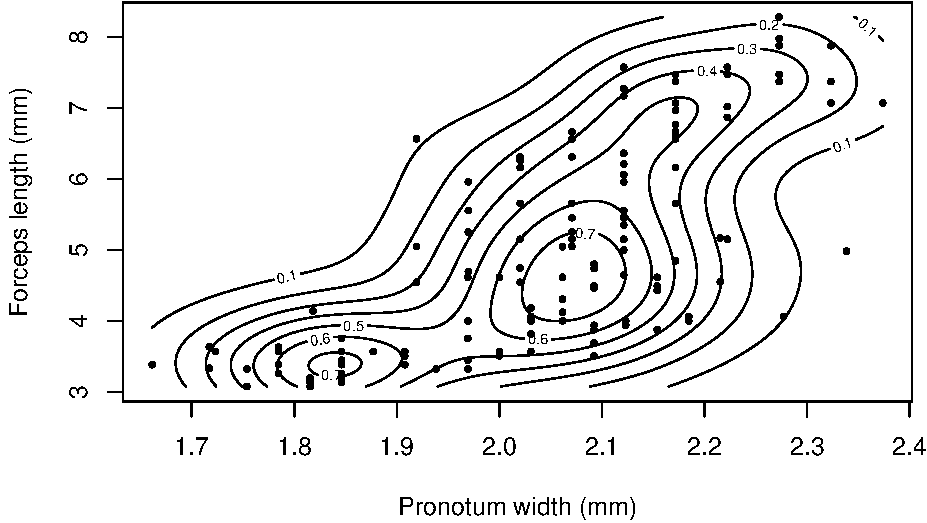
\includegraphics{3rd_Edition_files/figure-latex/unnamed-chunk-272-1.pdf}
\caption{\label{fig:unnamed-chunk-272}Contour plot of earwig forceps length versus pronotum width with individual data points added.}
\end{figure}

I'm not sure if this graph really helps us understand the allometry of forceps length in male earwigs on Brownsman Island, but at least it looks nice.

\begin{center}\rule{0.5\linewidth}{0.5pt}\end{center}

\hypertarget{exporting-graphics}{%
\section{Exporting Graphics}\label{exporting-graphics}}

There are lots of different image formats, and R runs on a number of different platforms that use different graphics formats in different ways. It shouldn't surprise you then to find out that there are lots of different options for exporting your graphics from R. If you're using Windows or a Mac then there is an easy way that doesn't give you much control, or there is a hard way that gives you more control. In Linux there's only the hard way.

\hypertarget{the-easy-way}{%
\subsection{The easy way}\label{the-easy-way}}

If you're using either Windows or a Mac, then draw your graph and select the window that it's drawn in. You can then use the ``Save as'' option from the ``File'' pull-down menu to save your graph. If you're exporting a graph in Windows, you get a variety of choices of format, the best one of which may be a .wmf (Windows meta-file). This is a vector graphics format so you can import it to another package and do things like resizing it without any trouble. On a Mac running OS X, R automatically exports graphs as pdfs. This is what it should do: pdf is the default graphics filetype in OS X, and gives nice crisp vector graphics again. The only problem is that if you're using MS Word it may well not import your pdfs nicely - the results vary by version but in general it makes them into pixellated bitmaps. If you're using a Mac and want to import your graphs to Word, you might have to do something like open them in Photoshop and save them as a high-res GIF or similar. Recent releases of Word are better at coping with pdfs but still not perfect.

\hypertarget{the-hard-way}{%
\subsection{The hard way}\label{the-hard-way}}

Using the pull-down menus as described above is easy but you don't have much control over things like the size of the saved image. The other option for saving graphs, using the command line (surprise!) gives you a lot more control over these details. If you want to export to one of the common graphic formats you can use one of these functions:
-\texttt{png()}
-\texttt{jpeg()}
-\texttt{tiff()}
-\texttt{bmp()}
-\texttt{pdf()}

The first four of these all work in very similar ways. \texttt{pdf()} is a bit more complex but works in basically the same way. To save a graphic with all of these functions it's a good idea to start by having your graph drawn nicely to your satisfaction and the code saved and accessible: either in the script editor or in a text editor somewhere. What you do might seem a bit strange if you're not used to it but there is some internal logic to the process, somewhere.

First, you use the command you've chosen to specify the filename to save the graph to. If you've decided to save to a .png, for example, you might type

\begin{Shaded}
\begin{Highlighting}[]
\KeywordTok{png}\NormalTok{(}\DataTypeTok{filename=}\NormalTok{“Figure1.png”)}
\end{Highlighting}
\end{Shaded}

If you've got it right then all you'll get when you hit return is the command prompt again. What you do now is paste in your code for drawing your figure. You can use as many lines of code as you need. Press enter again. If all is still well, you'll just get a command prompt again.

\begin{Shaded}
\begin{Highlighting}[]
\KeywordTok{plot}\NormalTok{(xvariable, yvariable, }\DataTypeTok{pch=}\DecValTok{16}\NormalTok{, }\DataTypeTok{xlab=}\NormalTok{“X axis”, }\DataTypeTok{ylab=}\NormalTok{“Y axis”)}
\KeywordTok{abline}\NormalTok{(}\OperatorTok{-}\DecValTok{2}\NormalTok{, }\DecValTok{3}\NormalTok{,}\DataTypeTok{lty=}\DecValTok{2}\NormalTok{)}
\end{Highlighting}
\end{Shaded}

Now you type the function \texttt{dev.off()}, which might cause some cryptic messages to appear

\begin{Shaded}
\begin{Highlighting}[]
\KeywordTok{dev.off}\NormalTok{()}
\NormalTok{quartz }
    \DecValTok{2}
\end{Highlighting}
\end{Shaded}

That's it. If all is well you can now look in your working directory (or another directory if you specified a file path rather than just a name) and you should find your graphics file there. What's going on? Why don't you see your graph, and what do these strange functions do? To understand this process you need to know that R draws graphs in things it calls ``devices''. There is an active, current device and any graphics functions called will draw what they're told to draw in that device. Normally this will be a window, and the graphics code you use will draw things in the window where you can see it, but when you use a function like \texttt{png()} you tell R to open a new device, which is effectively the graphics file that you're writing to. When you put in your graphics code after opening a new device that isn't a graph window, you don't see the new graph because it's not being written to the window. Then, when you type \texttt{dev.off()} that closes whichever device is the active device and in the case of your graphics file write the file to the appropriate directory. See? I said there was some logic. If that doesn't make any sense to you then don't worry.
Why should you go through the trouble and confusion of saving your graphics in this apparently baroque and perverse fashion? Because it gives you a huge amount of control over the final graphics file. You can add arguments to functions like \texttt{png()} that will determine precisely the size of the image, the size of the text, the colour of the background and even whether there's a background at all. Let's say that you want a graph with dimensions 560 by 340 pixels with 24 point text as the default (which can be altered by the \texttt{cex\ldots{}} arguments in \texttt{plot()} etc). Let's also go for a transparent background so that you can use your graph in your latest powerpoint presentation with some bad-taste background image showing through in the hope of distracting your audience from noticing how dodgy your correlation is.

\begin{Shaded}
\begin{Highlighting}[]
\KeywordTok{png}\NormalTok{(}\DataTypeTok{filename=}\NormalTok{“Figure1.png”, }\DataTypeTok{width=}\DecValTok{560}\NormalTok{, }\DataTypeTok{height=}\DecValTok{340}\NormalTok{, }\DataTypeTok{bg=}\StringTok{"transparent"}\NormalTok{, }\DataTypeTok{pointsize=}\DecValTok{24}\NormalTok{)}
\end{Highlighting}
\end{Shaded}

Will ensure that figure 1 comes out exactly how you want it.

\hypertarget{r-graphics-ii-adding-elements-to-an-existing-graph}{%
\chapter{R graphics II --- Adding elements to an existing graph}\label{r-graphics-ii-adding-elements-to-an-existing-graph}}

All the examples we've looked at in detail so far use arguments within the \texttt{plot()} function call to change the appearance of our graph, but we've also seen an example of using the \texttt{legend()} function to add something extra to an existing graph. R has quite a few functions which, like \texttt{legend()} can draw new elements onto existing graphs. These include:

\begin{longtable}[]{@{}ll@{}}
\toprule
Function & Purpose\tabularnewline
\midrule
\endhead
\texttt{points()} & Draws points onto a plot\tabularnewline
\texttt{lines()} & Draws lines\tabularnewline
\texttt{abline()} & Draws a line specified by intercept and slope\tabularnewline
\texttt{polygon()} & Draws a shape\tabularnewline
\texttt{arrows()} & Draws arrows on a plot\tabularnewline
\texttt{text()} & Adds text\tabularnewline
\texttt{mtext()} & Adds text in the plot margins\tabularnewline
\texttt{legend()} & Adds a legend\tabularnewline
\texttt{axis()} & Adds an axis\tabularnewline
\texttt{title()} & Adds a title or subtitle\tabularnewline
\bottomrule
\end{longtable}

These functions will all add elements to the plot which is currently displayed in the graphics window, so you have to be a little careful about where you put the code. The best option is to use a script and have these functions directly after the \texttt{plot()} function call. Let's look at some examples.

\hypertarget{simple-regression-lines}{%
\section{Simple regression lines}\label{simple-regression-lines}}

Let's go back to our data on pinnipeds. If we plot the log of male brain size against the log of male mass then we see a positive relationship (big animals have bigger brains) that could be described reasonably well by a straight line:

\begin{Shaded}
\begin{Highlighting}[]

\NormalTok{pinniped <-}\StringTok{ }\KeywordTok{read.csv}\NormalTok{(}\StringTok{"http://www.introductoryr.co.uk/Pinniped_brains.csv"}\NormalTok{, }
                     \DataTypeTok{stringsAsFactors =} \OtherTok{FALSE}\NormalTok{)}

\KeywordTok{plot}\NormalTok{(}\KeywordTok{log}\NormalTok{(pinniped}\OperatorTok{$}\NormalTok{Male_brain) }\OperatorTok{~}\StringTok{ }\KeywordTok{log}\NormalTok{(pinniped}\OperatorTok{$}\NormalTok{Male_mass),}
     \DataTypeTok{xlab =} \StringTok{"Log male mass (Kg)"}\NormalTok{,}
     \DataTypeTok{ylab =} \StringTok{"Log male brain mass (g)"}\NormalTok{)}
\end{Highlighting}
\end{Shaded}

\begin{figure}
\centering
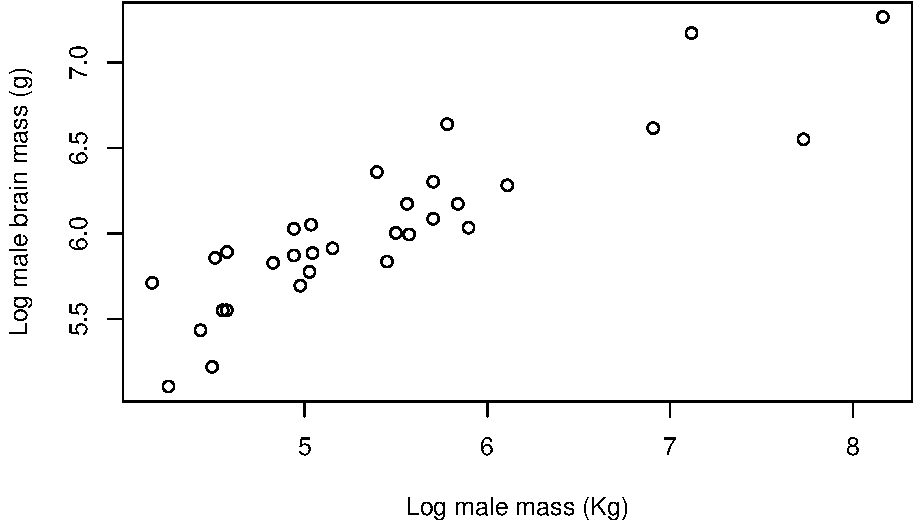
\includegraphics{3rd_Edition_files/figure-latex/unnamed-chunk-279-1.pdf}
\caption{\label{fig:unnamed-chunk-279}Log of brain size plotted against the log of body mass for male pinnipeds from 33 species}
\end{figure}

We can generate the slope and intercept of a fitted linear regression line using the \texttt{lm()} function. If you don't know what this is don't worry, the analysis is explained in chapter XX: for the moment all you need to know is that it's a way of generating a best-fit line.

\begin{Shaded}
\begin{Highlighting}[]
\KeywordTok{lm}\NormalTok{(}\KeywordTok{log}\NormalTok{(pinniped}\OperatorTok{$}\NormalTok{Male_brain) }\OperatorTok{~}\StringTok{ }\KeywordTok{log}\NormalTok{(pinniped}\OperatorTok{$}\NormalTok{Male_mass))}

\NormalTok{Call}\OperatorTok{:}
\KeywordTok{lm}\NormalTok{(}\DataTypeTok{formula =} \KeywordTok{log}\NormalTok{(pinniped}\OperatorTok{$}\NormalTok{Male_brain) }\OperatorTok{~}\StringTok{ }\KeywordTok{log}\NormalTok{(pinniped}\OperatorTok{$}\NormalTok{Male_mass))}

\NormalTok{Coefficients}\OperatorTok{:}
\StringTok{            }\NormalTok{(Intercept)  }\KeywordTok{log}\NormalTok{(pinniped}\OperatorTok{$}\NormalTok{Male_mass)  }
                  \FloatTok{3.672}                    \FloatTok{0.435}  
\end{Highlighting}
\end{Shaded}

So our intercept is 3.672 and our slope is 0.435. If we want to add this line to our plot we can use the \texttt{abline()} function which takes an intercept (``a'') and a slope (``b'') and draws a line:

\begin{Shaded}
\begin{Highlighting}[]

\KeywordTok{plot}\NormalTok{(}\KeywordTok{log}\NormalTok{(pinniped}\OperatorTok{$}\NormalTok{Male_brain) }\OperatorTok{~}\StringTok{ }\KeywordTok{log}\NormalTok{(pinniped}\OperatorTok{$}\NormalTok{Male_mass),}
     \DataTypeTok{xlab =} \StringTok{"Log male mass (Kg)"}\NormalTok{,}
     \DataTypeTok{ylab =} \StringTok{"Log male brain mass (g)"}\NormalTok{)}

\KeywordTok{abline}\NormalTok{(}\DataTypeTok{a =} \FloatTok{3.672}\NormalTok{, }\DataTypeTok{b =} \FloatTok{0.435}\NormalTok{,}
       \DataTypeTok{lwd =} \DecValTok{2}\NormalTok{,}
       \DataTypeTok{col =} \StringTok{"darkblue"}\NormalTok{)}
\end{Highlighting}
\end{Shaded}

\begin{figure}
\centering
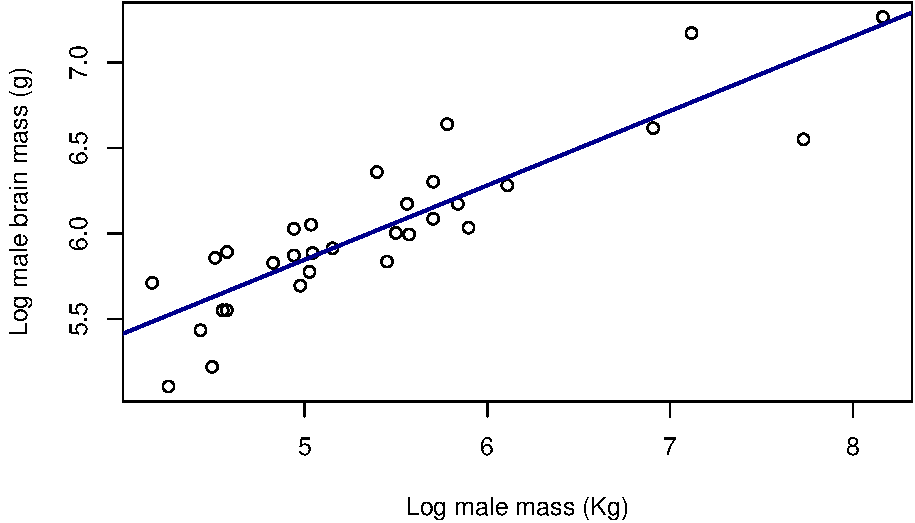
\includegraphics{3rd_Edition_files/figure-latex/unnamed-chunk-281-1.pdf}
\caption{\label{fig:unnamed-chunk-281}Log of brain size plotted against the log of body mass for male pinnipeds from 33 species. Line is a fitted linear regression.}
\end{figure}

Looking at that \texttt{abline()} call in a bit more detail you can see firstly that I've specified the slope and intercept with the \texttt{a\ =} and \texttt{b\ =} arguments. I've then asked for the line width to be twice the default width (\texttt{lwd\ =\ 2}) and finally I've used the \texttt{col\ =\ "darkblue"} argument to set the colour of the line.

\texttt{abline()} will actually take the coefficients directly from \texttt{lm()} if you are fitting a simple linear regression, either if you save the output from \texttt{lm()} and then give that to \texttt{abline()} as an argument or if you just put the whole \texttt{lm()} call within the \texttt{abline()} function call. So either of the following would have produced an identical line to the one we generated above:

\begin{Shaded}
\begin{Highlighting}[]
\CommentTok{# Save linear regression output as object "X1"}
\NormalTok{X1 <-}\StringTok{ }\KeywordTok{lm}\NormalTok{(}\KeywordTok{log}\NormalTok{(pinniped}\OperatorTok{$}\NormalTok{Male_brain) }\OperatorTok{~}\StringTok{ }\KeywordTok{log}\NormalTok{(pinniped}\OperatorTok{$}\NormalTok{Male_mass))}

\CommentTok{# Use object X1 in abline()}
\KeywordTok{abline}\NormalTok{(X1,}
      \DataTypeTok{lwd =} \DecValTok{2}\NormalTok{,}
      \DataTypeTok{col =} \StringTok{"darkblue"}\NormalTok{)}


\CommentTok{# Calculate linear regression directly within abline() function call}
\KeywordTok{abline}\NormalTok{(}\KeywordTok{lm}\NormalTok{(}\KeywordTok{log}\NormalTok{(pinniped}\OperatorTok{$}\NormalTok{Male_brain) }\OperatorTok{~}\StringTok{ }\KeywordTok{log}\NormalTok{(pinniped}\OperatorTok{$}\NormalTok{Male_mass)),}
      \DataTypeTok{lwd =} \DecValTok{2}\NormalTok{,}
      \DataTypeTok{col =} \StringTok{"darkblue"}\NormalTok{)}
\end{Highlighting}
\end{Shaded}

\texttt{abline()} will also add vertical or horizontal lines to a plot: if you use the \texttt{h\ =} argument then it will draw a horizontal line at the point on the y-axis specified, and \texttt{v\ =} will draw a vertical line at the point specified on the x axis. You can also use a vector of numbers if you want multiple horizontal or vertical lines.

The \texttt{lty\ =} parameter specifies the type of line drawn. Here are the various options:

Click here to see the code

\begin{Shaded}
\begin{Highlighting}[]
\KeywordTok{par}\NormalTok{(}\DataTypeTok{mar =} \KeywordTok{c}\NormalTok{(}\DecValTok{1}\NormalTok{,}\DecValTok{4}\NormalTok{,}\DecValTok{1}\NormalTok{,}\DecValTok{1}\NormalTok{))}
\KeywordTok{plot}\NormalTok{(}
  \DecValTok{1}\OperatorTok{:}\DecValTok{8}\NormalTok{,}
  \DecValTok{1}\OperatorTok{:}\DecValTok{8}\NormalTok{,}
  \DataTypeTok{type =} \StringTok{"n"}\NormalTok{,}
  \DataTypeTok{bty =} \StringTok{"n"}\NormalTok{,}
  \DataTypeTok{xaxt =} \StringTok{"n"}\NormalTok{,}
  \DataTypeTok{yaxt =} \StringTok{"n"}\NormalTok{,}
  \DataTypeTok{xlab =} \StringTok{""}\NormalTok{,}
  \DataTypeTok{ylab =} \StringTok{""}
\NormalTok{)}
\KeywordTok{abline}\NormalTok{(}\DataTypeTok{h =} \DecValTok{2}\OperatorTok{:}\DecValTok{7}\NormalTok{, }\DataTypeTok{lty =} \DecValTok{6}\OperatorTok{:}\DecValTok{1}\NormalTok{)}
\KeywordTok{axis}\NormalTok{(}
  \DataTypeTok{side =} \DecValTok{2}\NormalTok{,}
  \DataTypeTok{at =} \DecValTok{7}\OperatorTok{:}\DecValTok{2}\NormalTok{,}
  \DataTypeTok{labels =} \KeywordTok{c}\NormalTok{(}\StringTok{"lty = 1"}\NormalTok{, }\DecValTok{2}\NormalTok{, }\DecValTok{3}\NormalTok{, }\DecValTok{4}\NormalTok{, }\DecValTok{5}\NormalTok{, }\StringTok{"lty = 6"}\NormalTok{),}
  \DataTypeTok{tick =} \OtherTok{FALSE}\NormalTok{,}
  \DataTypeTok{lwd =} \DecValTok{0}\NormalTok{,}
  \DataTypeTok{las =} \DecValTok{1}
\NormalTok{)}
\KeywordTok{par}\NormalTok{(}\DataTypeTok{mar =} \KeywordTok{c}\NormalTok{(}\DecValTok{5}\NormalTok{,}\DecValTok{4}\NormalTok{,}\DecValTok{4}\NormalTok{,}\DecValTok{2}\NormalTok{) }\OperatorTok{+}\StringTok{ }\FloatTok{0.1}\NormalTok{)}
\end{Highlighting}
\end{Shaded}

\begin{figure}
\centering
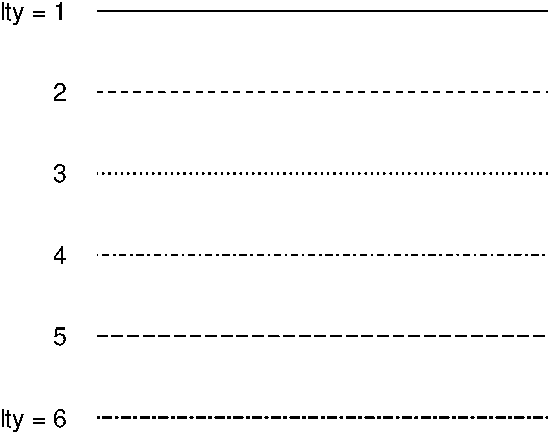
\includegraphics{3rd_Edition_files/figure-latex/unnamed-chunk-284-1.pdf}
\caption{\label{fig:unnamed-chunk-284}The different line types available in base R graphics}
\end{figure}

\hypertarget{multiple-regression-lines}{%
\section{Multiple regression lines}\label{multiple-regression-lines}}

You might recall from the last chapter that we divided our pinniped species by mating system into harem breeders, where males defend groups of females in the mating season, and non-harem breeders, where males only associate with a single female. We plotted our data with colours defined by a new factor that we generated called \texttt{Mating\_system} and it looked as though the relationship between log brain size and log body mass in males varied somewhat between the two groups. Let's look at that plot again.

\begin{Shaded}
\begin{Highlighting}[]

\NormalTok{Mating_system <-}
\StringTok{  }\KeywordTok{factor}\NormalTok{(}\KeywordTok{ifelse}\NormalTok{(pinniped}\OperatorTok{$}\NormalTok{Harem }\OperatorTok{==}\StringTok{ }\DecValTok{1}\NormalTok{, }\StringTok{"Non harem"}\NormalTok{, }\StringTok{"Harem"}\NormalTok{))}

\NormalTok{colours <-}\StringTok{ }\KeywordTok{c}\NormalTok{(}\StringTok{"aquamarine4"}\NormalTok{, }\StringTok{"chocolate2"}\NormalTok{)}

\KeywordTok{plot}\NormalTok{(}
  \KeywordTok{log}\NormalTok{(pinniped}\OperatorTok{$}\NormalTok{Male_brain) }\OperatorTok{~}\StringTok{ }\KeywordTok{log}\NormalTok{(pinniped}\OperatorTok{$}\NormalTok{Male_mass),}
  \DataTypeTok{xlab =} \StringTok{"Log body mass (Kg)"}\NormalTok{,}
  \DataTypeTok{ylab =} \StringTok{"Log brain mass (g)"}\NormalTok{,}
  \DataTypeTok{pch =} \DecValTok{16}\NormalTok{,}
  \DataTypeTok{col =}\NormalTok{ colours[Mating_system]}
\NormalTok{)}
\end{Highlighting}
\end{Shaded}

\begin{figure}
\centering
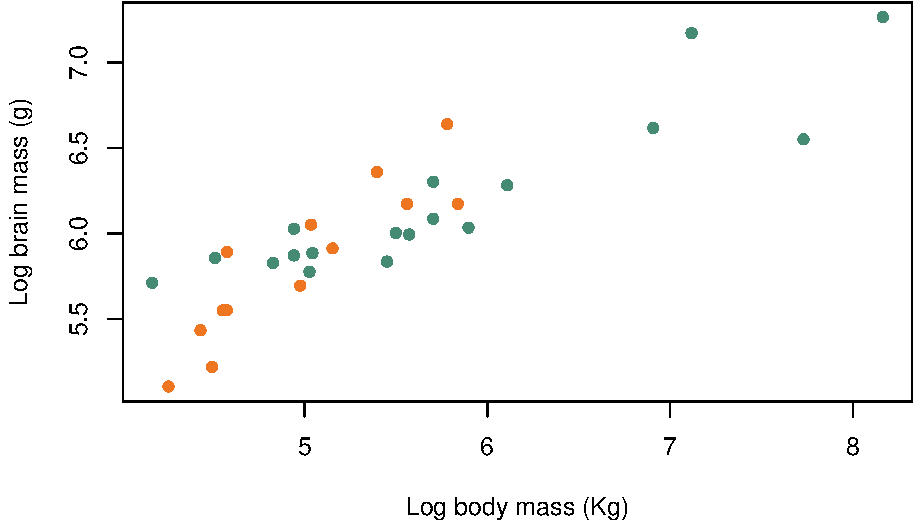
\includegraphics{3rd_Edition_files/figure-latex/unnamed-chunk-285-1.pdf}
\caption{\label{fig:unnamed-chunk-285}Brain mass versus body mass for 33 species of male pinniped plotted on log scaled axes, orange symbols indicate non-harem breeders and green indicate harem breeders}
\end{figure}

Maybe it would be helpful to draw in separate fitted lines for both mating systems. First we need to calculate the slopes and intercepts of the two fitted lines. If we were doing this as part of a formal analysis we'd do it all in one go with a general linear model with the mating system as a factor in the model, but for the sake of simplicity here we'll just run two linear regressions and use the \texttt{subset\ =} argument to specify which mating system we're using.

\begin{Shaded}
\begin{Highlighting}[]
\CommentTok{#Linear regression for harem breeders}
\NormalTok{harem_mod <-}
\StringTok{  }\KeywordTok{lm}\NormalTok{(}\KeywordTok{log}\NormalTok{(Male_brain) }\OperatorTok{~}\StringTok{ }\KeywordTok{log}\NormalTok{(Male_mass),}
     \DataTypeTok{data =}\NormalTok{ pinniped,}
     \DataTypeTok{subset =}\NormalTok{ Mating_system }\OperatorTok{==}\StringTok{ "Harem"}\NormalTok{)}

\CommentTok{#Linear regression for non harem breeders}
\NormalTok{non_harem_mod <-}
\StringTok{  }\KeywordTok{lm}\NormalTok{(}\KeywordTok{log}\NormalTok{(Male_brain) }\OperatorTok{~}\StringTok{ }\KeywordTok{log}\NormalTok{(Male_mass),}
     \DataTypeTok{data =}\NormalTok{ pinniped,}
     \DataTypeTok{subset =}\NormalTok{ Mating_system }\OperatorTok{==}\StringTok{ "Non harem"}\NormalTok{)}

\CommentTok{#Slope and intercept for harem breeders}
\KeywordTok{coef}\NormalTok{(harem_mod)}
\NormalTok{   (Intercept) }\KeywordTok{log}\NormalTok{(Male_mass) }
       \FloatTok{4.00515}        \FloatTok{0.37765} 

\CommentTok{#Slope and intercept for non-harem breeders}
\KeywordTok{coef}\NormalTok{(non_harem_mod)}
\NormalTok{   (Intercept) }\KeywordTok{log}\NormalTok{(Male_mass) }
       \FloatTok{2.07789}        \FloatTok{0.75439} 
\end{Highlighting}
\end{Shaded}

Now we can add these fitted lines to our plot. One option, and by far the easiest, is to use \texttt{abline()}.

\begin{Shaded}
\begin{Highlighting}[]

\KeywordTok{plot}\NormalTok{(}\KeywordTok{log}\NormalTok{(pinniped}\OperatorTok{$}\NormalTok{Male_brain) }\OperatorTok{~}\StringTok{ }\KeywordTok{log}\NormalTok{(pinniped}\OperatorTok{$}\NormalTok{Male_mass),}
     \DataTypeTok{xlab =} \StringTok{"Log body mass (Kg)"}\NormalTok{,}
     \DataTypeTok{ylab =} \StringTok{"Log brain mass (g)"}\NormalTok{, }
     \DataTypeTok{pch =} \DecValTok{16}\NormalTok{,}
     \DataTypeTok{col =}\NormalTok{ colours[Mating_system])}

\KeywordTok{abline}\NormalTok{(harem_mod, }\DataTypeTok{col =}\NormalTok{ colours[}\DecValTok{1}\NormalTok{], }\DataTypeTok{lwd =} \DecValTok{2}\NormalTok{)}
\KeywordTok{abline}\NormalTok{(non_harem_mod, }\DataTypeTok{col =}\NormalTok{ colours[}\DecValTok{2}\NormalTok{], }\DataTypeTok{lwd =} \DecValTok{2}\NormalTok{)}
\end{Highlighting}
\end{Shaded}

\begin{figure}
\centering
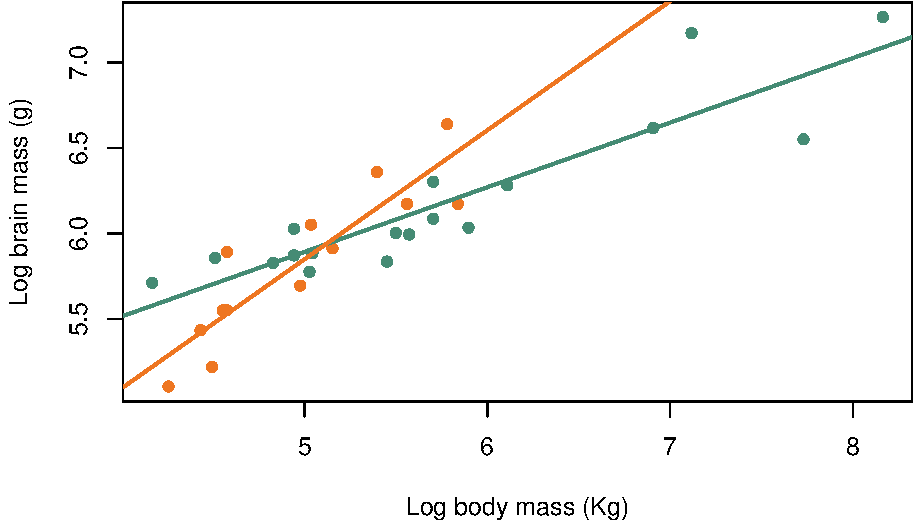
\includegraphics{3rd_Edition_files/figure-latex/unnamed-chunk-287-1.pdf}
\caption{\label{fig:unnamed-chunk-287}Brain mass versus body mass for 33 species of male pinniped plotted on log scaled axes, orange symbols indicate non-harem breeders and green indicate harem breeders. Lines indicate fitted linear regressions.}
\end{figure}

That's OK\ldots{} but not fantastic. The fitted lines go across the whole of the graph and in the case of the non-harem breeders especially end up a long way outside the limits of the data we've fitted them to. It would be much better to only draw the lines within the minima and maxima of the data we've used. There are a variety of ways to do this: we can use the \texttt{clip()} function to make sure that \texttt{abline()} draws within the area we want, or we can draw our fitted lines using the \texttt{lines()} function. The latter is probably the most common way to do this so we'll do it first but it's also a bit more complicated than using \texttt{clip()}. \texttt{lines()} draws lines between specified x and y coordinates on a plot, so we need to know the minimum and maximum x values for our two groups of data and then calculate the y values for the lines corresponding to those data points. We can extract these values using the \texttt{min()} and \texttt{max()} functions, or we can do it in one go with the \texttt{summary()} function.

We need to remember to use \texttt{log()} to transform our data and also to use a subscript to specify that we only want the data points for which \texttt{Mating\_system\ ==\ "Harem"} is \texttt{TRUE}.Here's what we get from \texttt{summary()}:

\begin{Shaded}
\begin{Highlighting}[]
\KeywordTok{summary}\NormalTok{(}\KeywordTok{log}\NormalTok{(pinniped}\OperatorTok{$}\NormalTok{Male_mass[Mating_system }\OperatorTok{==}\StringTok{ "Harem"}\NormalTok{]))}
\NormalTok{   Min. 1st Qu.  Median    Mean 3rd Qu.    Max. }
   \FloatTok{4.17}    \FloatTok{4.94}    \FloatTok{5.50}    \FloatTok{5.69}    \FloatTok{6.00}    \FloatTok{8.16} 
\end{Highlighting}
\end{Shaded}

So we can generate a vector with the minimum and maximum values for x for harem breeders

\begin{Shaded}
\begin{Highlighting}[]

\NormalTok{harem_x <-}\StringTok{ }\KeywordTok{c}\NormalTok{(}\FloatTok{4.17}\NormalTok{, }\FloatTok{8.16}\NormalTok{)}
\end{Highlighting}
\end{Shaded}

For non-harem breeders:

\begin{Shaded}
\begin{Highlighting}[]
\KeywordTok{summary}\NormalTok{(}\KeywordTok{log}\NormalTok{(pinniped}\OperatorTok{$}\NormalTok{Male_mass[Mating_system }\OperatorTok{==}\StringTok{ "Non harem"}\NormalTok{]))}
\NormalTok{   Min. 1st Qu.  Median    Mean 3rd Qu.    Max. }
   \FloatTok{4.26}    \FloatTok{4.56}    \FloatTok{5.01}    \FloatTok{5.03}    \FloatTok{5.52}    \FloatTok{5.84} 

\NormalTok{non_harem_x <-}\StringTok{ }\KeywordTok{c}\NormalTok{(}\FloatTok{4.26}\NormalTok{, }\FloatTok{5.84}\NormalTok{)}
\end{Highlighting}
\end{Shaded}

Now we need to calculate the corresponding y values and we can draw our lines. We know that the equations for our two lines are

\begin{Shaded}
\begin{Highlighting}[]
\NormalTok{harem_y <-}\StringTok{ }\KeywordTok{coef}\NormalTok{(harem_mod)[}\DecValTok{1}\NormalTok{] }\OperatorTok{+}\StringTok{ }\KeywordTok{coef}\NormalTok{(harem_mod)[}\DecValTok{2}\NormalTok{] }\OperatorTok{*}\StringTok{ }\NormalTok{harem_x}
\NormalTok{non_harem_y <-}\StringTok{ }\KeywordTok{coef}\NormalTok{(non_harem_mod)[}\DecValTok{1}\NormalTok{] }\OperatorTok{+}\StringTok{ }\KeywordTok{coef}\NormalTok{(non_harem_mod)[}\DecValTok{2}\NormalTok{] }\OperatorTok{*}\StringTok{ }\NormalTok{non_harem_x}
\end{Highlighting}
\end{Shaded}

Now we can use `lines()' to draw the two regression lines onto our plot.

\begin{Shaded}
\begin{Highlighting}[]

\KeywordTok{plot}\NormalTok{(}\KeywordTok{log}\NormalTok{(pinniped}\OperatorTok{$}\NormalTok{Male_brain) }\OperatorTok{~}\StringTok{ }\KeywordTok{log}\NormalTok{(pinniped}\OperatorTok{$}\NormalTok{Male_mass),}
     \DataTypeTok{xlab =} \StringTok{"Log body mass (Kg)"}\NormalTok{,}
     \DataTypeTok{ylab =} \StringTok{"Log brain mass (g)"}\NormalTok{, }
     \DataTypeTok{pch =} \DecValTok{16}\NormalTok{,}
     \DataTypeTok{col =}\NormalTok{ colours[Mating_system])}

\KeywordTok{lines}\NormalTok{(}\DataTypeTok{x =}\NormalTok{ harem_x, }\DataTypeTok{y =}\NormalTok{ harem_y, }\DataTypeTok{col =}\NormalTok{ colours[}\DecValTok{1}\NormalTok{], }\DataTypeTok{lwd =} \DecValTok{2}\NormalTok{)}
\KeywordTok{lines}\NormalTok{(}\DataTypeTok{x =}\NormalTok{ non_harem_x, }\DataTypeTok{y =}\NormalTok{ non_harem_y, }\DataTypeTok{col =}\NormalTok{ colours[}\DecValTok{2}\NormalTok{], }\DataTypeTok{lwd =} \DecValTok{2}\NormalTok{)}
\end{Highlighting}
\end{Shaded}

\begin{figure}
\centering
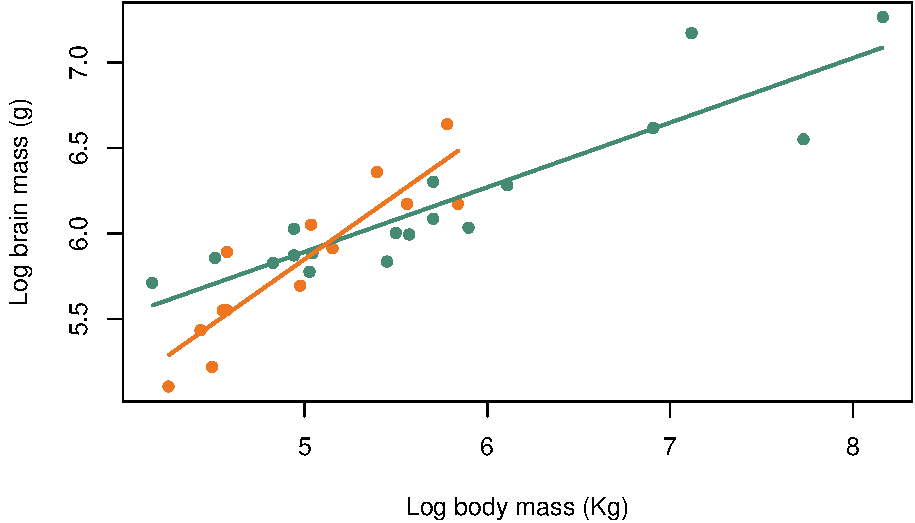
\includegraphics{3rd_Edition_files/figure-latex/unnamed-chunk-292-1.pdf}
\caption{\label{fig:unnamed-chunk-292}Brain mass versus body mass for 33 species of male pinniped plotted on log scaled axes, orange symbols indicate non-harem breeders and green indicate harem breeders. Lines indicate fitted linear regressions.}
\end{figure}

That's a much more acceptable plot than the previous version and we are not extrapolating our lines beyond the limits of the data that they are calculated from. How about using \texttt{clip()} and \texttt{abline()} to do the same thing? What you need to know here is that \texttt{clip()} sets the area of the graph on which it is possible to draw things like lines, points and text. This is normally simply defined by the limits of the x- and y-axes, but we can define our own area if necessary. \texttt{clip()} takes four arguments, x1, x2, y1 and y2 which are the lower and upper limits of the clip region in x- and y-coordinates respectively, and you need to supply all of them: there are no defaults. We already have the minimum and maximum x-values calculated for harem and non-harem breeders, and for the y-values we'll just use a small minimum and a big maximum since we're not concerned about those as limits for our line. We have to set a different clip area for each line, of course.

\begin{Shaded}
\begin{Highlighting}[]

\KeywordTok{plot}\NormalTok{(}\KeywordTok{log}\NormalTok{(pinniped}\OperatorTok{$}\NormalTok{Male_brain) }\OperatorTok{~}\StringTok{ }\KeywordTok{log}\NormalTok{(pinniped}\OperatorTok{$}\NormalTok{Male_mass),}
     \DataTypeTok{xlab =} \StringTok{"Log body mass (Kg)"}\NormalTok{,}
     \DataTypeTok{ylab =} \StringTok{"Log brain mass (g)"}\NormalTok{, }
     \DataTypeTok{pch =} \DecValTok{16}\NormalTok{,}
     \DataTypeTok{col =}\NormalTok{ colours[Mating_system])}

\KeywordTok{clip}\NormalTok{(}\DataTypeTok{x1 =}\NormalTok{ harem_x[}\DecValTok{1}\NormalTok{], }\DataTypeTok{x2 =}\NormalTok{ harem_x[}\DecValTok{2}\NormalTok{], }\DataTypeTok{y1 =} \DecValTok{4}\NormalTok{, }\DataTypeTok{y2 =} \DecValTok{8}\NormalTok{)}
\KeywordTok{abline}\NormalTok{(harem_mod, }\DataTypeTok{col =}\NormalTok{ colours[}\DecValTok{1}\NormalTok{], }\DataTypeTok{lwd =} \DecValTok{2}\NormalTok{)}

\KeywordTok{clip}\NormalTok{(}\DataTypeTok{x1 =}\NormalTok{ non_harem_x[}\DecValTok{1}\NormalTok{], }\DataTypeTok{x2 =}\NormalTok{ non_harem_x[}\DecValTok{2}\NormalTok{], }\DataTypeTok{y1 =} \DecValTok{4}\NormalTok{, }\DataTypeTok{y2 =} \DecValTok{8}\NormalTok{)}
\KeywordTok{abline}\NormalTok{(non_harem_mod, }\DataTypeTok{col =}\NormalTok{ colours[}\DecValTok{2}\NormalTok{], }\DataTypeTok{lwd =} \DecValTok{2}\NormalTok{)}
\end{Highlighting}
\end{Shaded}

\begin{figure}
\centering
\includegraphics{3rd_Edition_files/figure-latex/unnamed-chunk-293-1.pdf}
\caption{\label{fig:unnamed-chunk-293}Brain mass versus body mass for 33 species of male pinniped plotted on log scaled axes, orange symbols indicate non-harem breeders and green indicate harem breeders. Lines indicate fitted linear regressions.}
\end{figure}

There we go, the exact same graph as before but generated in a rather different way. One thing that's really important to remember when using \texttt{clip()} is that the clipping region will stay as the area you've specified if you want to add anything else, say a legend, to your plot. If you want to return to the default clipping area you can use this code:

\begin{Shaded}
\begin{Highlighting}[]
\KeywordTok{do.call}\NormalTok{(}\StringTok{"clip"}\NormalTok{, }\KeywordTok{as.list}\NormalTok{(}\KeywordTok{par}\NormalTok{(}\StringTok{"usr"}\NormalTok{)))}
\end{Highlighting}
\end{Shaded}

\texttt{par("usr")} gives the original clipping region of the graph as defined by the x- and y-axis minima and maxima. \texttt{do.call()} is a function which will execute a specified function from the name of the function and a list of the arguments to be passed to it, so we use \texttt{as.list()} to convert the output from \texttt{par("usr")} to a list and use the \texttt{do.call()} function with ``clip'' as the first argument. The alternative would be to do something like this:

\begin{Shaded}
\begin{Highlighting}[]
\NormalTok{x1 <-}\StringTok{ }\KeywordTok{par}\NormalTok{(}\StringTok{"usr"}\NormalTok{)}
\KeywordTok{clip}\NormalTok{(}\DataTypeTok{x1 =}\NormalTok{ x1[}\DecValTok{1}\NormalTok{], }\DataTypeTok{x2 =}\NormalTok{ x1[}\DecValTok{2}\NormalTok{], }\DataTypeTok{y1 =}\NormalTok{ x1[}\DecValTok{3}\NormalTok{], }\DataTypeTok{y2 =}\NormalTok{ x1[}\DecValTok{4}\NormalTok{])}
\end{Highlighting}
\end{Shaded}

which is maybe a bit clunkier but also simpler and will do exactly the same.

\hypertarget{legends}{%
\section{Legends}\label{legends}}

Our plot needs a legend to let the reader know what the colour coding means. We've already seen one example of adding a legend in the previous chapter, but let's take another look.

\begin{Shaded}
\begin{Highlighting}[]
\KeywordTok{plot}\NormalTok{(}\KeywordTok{log}\NormalTok{(pinniped}\OperatorTok{$}\NormalTok{Male_brain) }\OperatorTok{~}\StringTok{ }\KeywordTok{log}\NormalTok{(pinniped}\OperatorTok{$}\NormalTok{Male_mass),}
     \DataTypeTok{xlab =} \StringTok{"Log body mass (Kg)"}\NormalTok{,}
     \DataTypeTok{ylab =} \StringTok{"Log brain mass (g)"}\NormalTok{, }
     \DataTypeTok{pch =} \DecValTok{16}\NormalTok{,}
     \DataTypeTok{col =}\NormalTok{ colours[Mating_system])}

\KeywordTok{clip}\NormalTok{(harem_x[}\DecValTok{1}\NormalTok{], harem_x[}\DecValTok{2}\NormalTok{], }\DecValTok{4}\NormalTok{,}\DecValTok{8}\NormalTok{)}
\KeywordTok{abline}\NormalTok{(harem_mod, }\DataTypeTok{col =}\NormalTok{ colours[}\DecValTok{1}\NormalTok{], }\DataTypeTok{lwd =} \DecValTok{2}\NormalTok{)}

\KeywordTok{clip}\NormalTok{(non_harem_x[}\DecValTok{1}\NormalTok{], non_harem_x[}\DecValTok{2}\NormalTok{], }\DecValTok{4}\NormalTok{,}\DecValTok{8}\NormalTok{)}
\KeywordTok{abline}\NormalTok{(non_harem_mod, }\DataTypeTok{col =}\NormalTok{ colours[}\DecValTok{2}\NormalTok{], }\DataTypeTok{lwd =} \DecValTok{2}\NormalTok{)}

\KeywordTok{do.call}\NormalTok{(}\StringTok{"clip"}\NormalTok{, }\KeywordTok{as.list}\NormalTok{(}\KeywordTok{par}\NormalTok{(}\StringTok{"usr"}\NormalTok{)))}

\KeywordTok{legend}\NormalTok{(}\StringTok{"topleft"}\NormalTok{,}
  \DataTypeTok{legend =} \KeywordTok{c}\NormalTok{(}\StringTok{"Harem"}\NormalTok{, }\StringTok{"Non harem"}\NormalTok{),}
  \DataTypeTok{col =}\NormalTok{ colours,}
  \DataTypeTok{pch  =} \DecValTok{16}\NormalTok{,}
  \DataTypeTok{lty =} \DecValTok{1}\NormalTok{,}
  \DataTypeTok{lwd =} \DecValTok{2}\NormalTok{,}
  \DataTypeTok{bty =} \StringTok{"n"}\NormalTok{,}
  \DataTypeTok{title =} \KeywordTok{expression}\NormalTok{(}\KeywordTok{bold}\NormalTok{(}\StringTok{"Mating system"}\NormalTok{)))}
\end{Highlighting}
\end{Shaded}

\begin{figure}
\centering
\includegraphics{3rd_Edition_files/figure-latex/graph11a-1.pdf}
\caption{\label{fig:graph11a}Brain mass versus body mass for 33 species of male pinniped plotted on log scaled axes, colour coded for mating system with legend}
\end{figure}

The first piece of code plots the data, then the second adds the legend. It's got quite a few arguments so let's run through them individually. \texttt{"topleft"} tells \texttt{legend()} where to put the legend. There are a number of options for this so \texttt{"bottomright"} would put it in the bottom right hand corner and \texttt{"top"} would place it in the middle of the top. You can find all the options if you look in the ``Details'' section of the \texttt{legend()} help file.

If you want to be specific about where your legend goes you can use x and y coordinates instead of text descriptions --- you might remember that in the previous chapter we used this along with setting \texttt{par(xdp)\ =\ TRUE)} to add a legend to the right of the plot area. Lots of the R functions which add elements to graphs use coordinates, and it's straightforward to use them because they are on the same scale that the points are plotted on. \texttt{legend()} puts the top left corner of the legend at the specified point so if you replaced \texttt{legend("topright",...} with \texttt{legend(x\ =\ 4.01,\ y\ =\ 7.35,...} you'd get a very similar result.

The confusingly-named argument \texttt{legend\ =} gives the text that goes in the legend, in this case as a character vector with two elements. \texttt{legend()} will generate a legend with one entry for each element in the vector, so in this case we'll get two entries. \texttt{col\ =\ colours} tells it what colours to associate with each entry, and then we specify both a plot symbol (\texttt{pch\ =\ 16}) and a line type and width (\texttt{lty\ =\ 1,\ lwd\ =\ 2}). This gives us both a line and a plot symbol in the appropriate colour. If we'd only specified a plot symbol or a line type then we'd only have got one of the two.

\texttt{bty\ =\ "n"} means that we have a legend without a box drawn around it. Finally we give a title for the legend: \texttt{title\ =\ expression(bold("Mating\ system"))}. If we just wanted this in standard text we would simply have input \texttt{title\ =\ "Mating\ system"} but it looks better to have this in bold. Consequently we're using the \texttt{expression()} function which gives us a lot of control over our text, and allows us to have the title in bold.

As an aside, for ``normal'' text on a plot such as axis labels we can specify bold or italic using one of the \texttt{font...} parameters as an argument, so if you want the axis labels in bold then \texttt{...,\ font.lab\ =\ 2} will do the trick, or if you want the main title in italics then \texttt{....,\ font.main\ =\ 3}. This doesn't work for text in a legend, however, so we have to use more complex methods.

\hypertarget{curves}{%
\section{Curves}\label{curves}}

\hypertarget{adding-a-curve-using-curve}{%
\subsection{\texorpdfstring{Adding a curve using \texttt{curve()}}{Adding a curve using curve()}}\label{adding-a-curve-using-curve}}

Very often, of course, relationships between two variables are best described by a curve rather than a straight line. We're going to abanodon the seals and sealions for a while because of a lack of suitable curves and go back to our World Bank data. Here's the relationship between a country's CO\textsubscript{2} emissions in metric tonnes per capita and the GNP per capita. Both of these are plotted on a log\textsubscript{10} scale.

\begin{Shaded}
\begin{Highlighting}[]
\NormalTok{logCO2 <-}\StringTok{ }\KeywordTok{log10}\NormalTok{(WB}\OperatorTok{$}\NormalTok{CO2)}
\NormalTok{logGNP <-}\StringTok{ }\KeywordTok{log10}\NormalTok{(WB}\OperatorTok{$}\NormalTok{GNP)}

\KeywordTok{plot}\NormalTok{(logCO2 }\OperatorTok{~}\StringTok{ }\NormalTok{logGNP,}
     \DataTypeTok{col =} \StringTok{"steelblue"}\NormalTok{,}
     \DataTypeTok{xlab =} \StringTok{"Log GNP per capita"}\NormalTok{,}
     \DataTypeTok{ylab =} \StringTok{"Log Carbon dioxide emissions per capita"}\NormalTok{)}
\end{Highlighting}
\end{Shaded}

\begin{figure}
\centering
\includegraphics{3rd_Edition_files/figure-latex/unnamed-chunk-297-1.pdf}
\caption{\label{fig:unnamed-chunk-297}CO2 emissions per capita versus GNP per capita by country}
\end{figure}

There's a clear decrease in the slope of the relationship as GNP per capita increases. There are a variety of possible ways to describe such a relationship but one of the simplest is to use a \emph{second order polynomial} also known as a \emph{quadratic} equation. These take the form

\[ y = \beta _{1} + \beta_{2}x + \beta_{3}x^{2} \]
and have the big advantage that since they are mathematically linear we can estimate them using a linear model rather than one of those tricksy non-linear ones.

\begin{Shaded}
\begin{Highlighting}[]
\CommentTok{# Fit model}
\NormalTok{poly1 <-}\StringTok{ }\KeywordTok{lm}\NormalTok{(logCO2 }\OperatorTok{~}\StringTok{ }\NormalTok{logGNP }\OperatorTok{+}\StringTok{ }\KeywordTok{I}\NormalTok{(logGNP}\OperatorTok{^}\DecValTok{2}\NormalTok{))}

\CommentTok{# Show coefficients}
\KeywordTok{coef}\NormalTok{(poly1)}
\NormalTok{(Intercept)      logGNP }\KeywordTok{I}\NormalTok{(logGNP}\OperatorTok{^}\DecValTok{2}\NormalTok{) }
   \FloatTok{-7.97986}     \FloatTok{3.53398}    \FloatTok{-0.34562} 
\end{Highlighting}
\end{Shaded}

We're not going to worry about the details of the model or whether it is statistically significant for the moment, we're just using it to produce estimates of our three coefficients. Now we know the formula for our curve, which is

\[ log_{10} \mathrm{CO}_{2} = -7.98 + 3.53 \times log_{10} \mathrm{GNP} - 0.346 \times log_{10} \mathrm{GNP} ^{2} \]
we can add it onto our graph. R being R of course there are many ways to do this: we can draw it in with \texttt{lines()}, we can draw it in with \texttt{points()} if we tell \texttt{points()} to draw a line,\footnote{Yes, we can do this, and we can also tell \texttt{lines()} to draw points --- both of them take the \texttt{type\ =} argument and can produce the full range of options: you can read about these in the help file for \texttt{plot.default}.} and we can add it to the plot using \texttt{curve()}.

Here's the last option, using \texttt{curve()}.

\begin{Shaded}
\begin{Highlighting}[]

\CommentTok{# Plot graph}
\KeywordTok{plot}\NormalTok{(logCO2 }\OperatorTok{~}\StringTok{ }\NormalTok{logGNP,}
     \DataTypeTok{col =} \StringTok{"steelblue"}\NormalTok{,}
     \DataTypeTok{xlab =} \StringTok{"Log GNP per capita"}\NormalTok{,}
     \DataTypeTok{ylab =} \StringTok{"Log Carbon dioxide emissions per capita"}\NormalTok{)}

\CommentTok{# Add curve}
\KeywordTok{curve}\NormalTok{(}\OperatorTok{-}\FloatTok{7.98} \OperatorTok{+}\StringTok{ }\FloatTok{3.53} \OperatorTok{*}\StringTok{ }\NormalTok{x }\FloatTok{-0.346} \OperatorTok{*}\StringTok{ }\NormalTok{x}\OperatorTok{^}\DecValTok{2}\NormalTok{,}
      \DataTypeTok{lwd =} \DecValTok{2}\NormalTok{,}
      \DataTypeTok{col =} \StringTok{"cadetblue4"}\NormalTok{,}
      \DataTypeTok{add =} \OtherTok{TRUE}\NormalTok{)}
\end{Highlighting}
\end{Shaded}

\begin{figure}
\centering
\includegraphics{3rd_Edition_files/figure-latex/unnamed-chunk-299-1.pdf}
\caption{\label{fig:unnamed-chunk-299}CO2 emissions per capita versus GNP per capita by country. Line shows a fitted quadratic curve}
\end{figure}

Quadratic curves are fairly simple beasts and in particular the rate at which the slope changes is constant across the whole thing, so the fit heere is really surprisingly good. Let's look at that \texttt{curve()} function call in a bit more detail.

\begin{Shaded}
\begin{Highlighting}[]
\KeywordTok{curve}\NormalTok{(}\OperatorTok{-}\FloatTok{7.98} \OperatorTok{+}\StringTok{ }\FloatTok{3.53} \OperatorTok{*}\StringTok{ }\NormalTok{x }\FloatTok{-0.346} \OperatorTok{*}\StringTok{ }\NormalTok{x}\OperatorTok{^}\DecValTok{2}\NormalTok{,}
      \DataTypeTok{lwd =} \DecValTok{2}\NormalTok{,}
      \DataTypeTok{col =} \StringTok{"cadetblue4"}\NormalTok{,}
      \DataTypeTok{add =} \OtherTok{TRUE}\NormalTok{)}
\end{Highlighting}
\end{Shaded}

The first argument is the actual formula of the curve we'd like to draw. This is only the right hand side of the equation: the \emph{y = } bit is assumed to be there. It's written out using the normal R arithmetic operators and is hopefully self explanatory. We then specify the width of the line as twice the default option \texttt{lwd\ =\ 2} and set the colour. The last argument is an important one: \texttt{add\ =\ TRUE}. This is needed because \texttt{curve()} is not a function like \texttt{lines()} or \texttt{text()} that adds elements to existing graphs by default: rather it draws a new graph in the same way that \texttt{plot()} would unless we tell it to add what it's drawing to an existing graph.

\hypertarget{adding-a-curve-using-lines-or-points.}{%
\subsection{\texorpdfstring{Adding a curve using \texttt{lines()} or \texttt{points()}.}{Adding a curve using lines() or points().}}\label{adding-a-curve-using-lines-or-points.}}

Here's another data set. We're moving from the world of CO\textsubscript{2} emissions measured on a national scale to thinking about the weapons used by male beetles when they fight over females.

\begin{Shaded}
\begin{Highlighting}[]
\NormalTok{beetle<-}\KeywordTok{read.table}\NormalTok{(}\StringTok{"http://www.introductoryr.co.uk/beetles.txt"}\NormalTok{,}\DataTypeTok{header=}\NormalTok{T)}
\end{Highlighting}
\end{Shaded}

The beetle dataset has horn length and body size (as measured across the pronotum, the first segment of the thorax) measurements for two species of dung beetle, \emph{Euoniticellus intermedius} and \emph{Onthophagus taurus}. We'll look at the latter at the moment. \emph{O. taurus} is an insect which has been heavily studied by behavioural ecologists because the males develop into two types: ``minor'' males with small or no horns, which acquire matings without aggression using what are called ``sneaky'' tactics, and ``major'' males which develop horns and who guard females and fight with other males in order to monopolise access to them. Whether a male develops into a minor or a major depends on its body size, and if we plot horn length against body size we get a sigmoid relationship.

\begin{Shaded}
\begin{Highlighting}[]

\KeywordTok{plot}\NormalTok{(beetle}\OperatorTok{$}\NormalTok{taurus_horn }\OperatorTok{~}\StringTok{ }\NormalTok{beetle}\OperatorTok{$}\NormalTok{taurus_pron,}
     \DataTypeTok{col =} \StringTok{"aquamarine4"}\NormalTok{,}
     \DataTypeTok{xlab =} \StringTok{"Pronotum width (mm)"}\NormalTok{,}
     \DataTypeTok{ylab =} \StringTok{"Horn length (mm)"}\NormalTok{)}
\end{Highlighting}
\end{Shaded}

\includegraphics{3rd_Edition_files/figure-latex/unnamed-chunk-302-1.pdf}
You can see that there is a ``switchpoint'' at a pronotum width of roughly 4.8mm, with beetles below this size having very reduced horns and beetles above this size having large horns. We'd like to draw a curve through these data to indicate the shape of the relationship. One option is to fit an equation of the form:

\[ horn \: length  = y_{0} + \frac{a \times body \: size^{b}}{c^{b} + body \: size^{b}}. \]

To do this we need to carry out a non-linear fit, which we don't need to go into the details of. Just trust me when I say that our fitted model gives a set of estimates for the coefficients of:

\emph{y\textsubscript{0}} = 0.41,\\
\emph{a} = 3.99,\\
\emph{b} = 45.76 \&\\
\emph{c} = 5.01,

giving us an equation for our curve of:

\[ horn \: length  = 0.41 + \frac{3.99 \times body \: size^{45.76}}{5.01^{45.76} + body \: size^{45.76}}. \]

We could draw this in using \texttt{curve()} but instead we're going to use a different method. We'll start by setting up a dummy x-variable with a sequence of points running from the minimum and maximum points where you want the curve to run from and to, and then we'll calculate the corresponding y-variables and draw them in with \texttt{lines()}. Previously we've used \texttt{lines()} to draw straight lines, but if you give it more than two x- and y- coordinates it will connect them together. Because we're using 200 points what is drawn comes out looking like a smooth curve. Note that you can get the exact same result by using \texttt{points()}, with the \texttt{type} argument set to \texttt{type="l"}\ldots{} which makes it draw lines.

Here is our dummy x-variable.

\begin{Shaded}
\begin{Highlighting}[]
\NormalTok{X1 <-}
\StringTok{  }\KeywordTok{seq}\NormalTok{(}
    \DataTypeTok{from =} \KeywordTok{min}\NormalTok{(beetle}\OperatorTok{$}\NormalTok{taurus_pron, }\DataTypeTok{na.rm =} \OtherTok{TRUE}\NormalTok{),}
    \DataTypeTok{to =} \KeywordTok{max}\NormalTok{(beetle}\OperatorTok{$}\NormalTok{taurus_pron, }\DataTypeTok{na.rm =} \OtherTok{TRUE}\NormalTok{),}
    \DataTypeTok{length =} \DecValTok{200}
\NormalTok{  )}
\end{Highlighting}
\end{Shaded}

This will give us 200 evenly spaced numbers across the range of pronotum widths. Now we need to work out the corresponding y values.

\begin{Shaded}
\begin{Highlighting}[]
\NormalTok{Y1 <-}\StringTok{ }\FloatTok{0.41} \OperatorTok{+}\StringTok{ }\NormalTok{(}\FloatTok{3.99} \OperatorTok{*}\StringTok{ }\NormalTok{(X1 }\OperatorTok{^}\StringTok{ }\FloatTok{45.76}\NormalTok{)) }\OperatorTok{/}\StringTok{ }\NormalTok{(}\FloatTok{5.01} \OperatorTok{^}\StringTok{ }\FloatTok{45.76} \OperatorTok{+}\StringTok{ }\NormalTok{(X1 }\OperatorTok{^}\StringTok{ }\FloatTok{45.76}\NormalTok{))}
\end{Highlighting}
\end{Shaded}

Finally, we can re-plot our graph and draw in the curve using \texttt{lines()}.

\begin{Shaded}
\begin{Highlighting}[]
\KeywordTok{plot}\NormalTok{(beetle}\OperatorTok{$}\NormalTok{taurus_horn }\OperatorTok{~}\StringTok{ }\NormalTok{beetle}\OperatorTok{$}\NormalTok{taurus_pron,}
     \DataTypeTok{col =} \StringTok{"aquamarine4"}\NormalTok{,}
     \DataTypeTok{xlab =} \StringTok{"Pronotum width (mm)"}\NormalTok{,}
     \DataTypeTok{ylab =} \StringTok{"Horn length (mm)"}\NormalTok{)}

\KeywordTok{lines}\NormalTok{(X1,Y1)}
\end{Highlighting}
\end{Shaded}

\begin{figure}
\centering
\includegraphics{3rd_Edition_files/figure-latex/unnamed-chunk-305-1.pdf}
\caption{\label{fig:unnamed-chunk-305}Horn length versus pronotum width for O. taurus with fitted curve}
\end{figure}

The first method we've seen for adding curves to a plot, using \texttt{curve()}, is simplest when you have a straightforward equation to describe your curve. The second comes in handy in lots of other situations though, such as when you have a complex model and you want to draw a line showing the fitted model. In this case you can use the \texttt{predict()} function to calculate your y values without having to worry about copying out all of the fitted model coefficients.

\hypertarget{text-and-arrows}{%
\section{Text and arrows}\label{text-and-arrows}}

Sometimes we want to add text to a plot, for example to indicate the identity of specific data points, or to show a specific event on a time series. Let's take a break from our pinnipeds data and look at a different data set: this is the relative number of Google searches for the term ``Springboks'' carried out in South Africa during the period September 1st to December 1st during the year 2019. For those who don't know, the Springboks are the South African rugby team and the Rugby World Cup was held in September, October and December of 2019. The data include dates, and we're going to use the \texttt{ymd()} function from the \emph{lubridate} package to convert the text which was downloaded from Google Trends into date formatted data for R.

\begin{Shaded}
\begin{Highlighting}[]
\CommentTok{# Load data}
\NormalTok{rugby <-}\StringTok{ }\KeywordTok{read.csv}\NormalTok{(}\StringTok{"Data/SA_Springboks_searches.csv"}\NormalTok{, }\DataTypeTok{stringsAsFactors =} \OtherTok{FALSE}\NormalTok{)}

\CommentTok{# Load lubridate package}
\KeywordTok{library}\NormalTok{(lubridate)}

\CommentTok{# Convert Week data to Date format}
\NormalTok{rugby}\OperatorTok{$}\NormalTok{Date <-}\StringTok{ }\KeywordTok{ymd}\NormalTok{(rugby}\OperatorTok{$}\NormalTok{Date)}

\KeywordTok{str}\NormalTok{(rugby)}
\StringTok{'data.frame'}\OperatorTok{:}\StringTok{   }\DecValTok{91}\NormalTok{ obs. of  }\DecValTok{2}\NormalTok{ variables}\OperatorTok{:}
\StringTok{ }\ErrorTok{$}\StringTok{ }\NormalTok{Date    }\OperatorTok{:}\StringTok{ }\NormalTok{Date, format}\OperatorTok{:}\StringTok{ "2019-09-01"} \StringTok{"2019-09-02"}\NormalTok{ ...}
 \OperatorTok{$}\StringTok{ }\NormalTok{Searches}\OperatorTok{:}\StringTok{ }\NormalTok{int  }\DecValTok{1} \DecValTok{1} \DecValTok{2} \DecValTok{2} \DecValTok{4} \DecValTok{24} \DecValTok{4} \DecValTok{2} \DecValTok{1} \DecValTok{1}\NormalTok{ ...}
\end{Highlighting}
\end{Shaded}

All looks good. Let's plot that out.

\begin{Shaded}
\begin{Highlighting}[]
\CommentTok{# Plot graph}
\KeywordTok{plot}\NormalTok{(rugby}\OperatorTok{$}\NormalTok{Searches }\OperatorTok{~}\StringTok{ }\NormalTok{rugby}\OperatorTok{$}\NormalTok{Date, }
     \DataTypeTok{type =} \StringTok{"l"}\NormalTok{, }
     \DataTypeTok{col =} \StringTok{"steelblue"}\NormalTok{, }
     \DataTypeTok{lwd =} \DecValTok{2}\NormalTok{,}
     \DataTypeTok{xlab =} \StringTok{"Date"}\NormalTok{,}
     \DataTypeTok{ylab =} \StringTok{"Search intensity on Google"}\NormalTok{,}
     \DataTypeTok{ylim =} \KeywordTok{c}\NormalTok{(}\DecValTok{0}\NormalTok{, }\DecValTok{120}\NormalTok{))}
\end{Highlighting}
\end{Shaded}

\begin{figure}
\centering
\includegraphics{3rd_Edition_files/figure-latex/unnamed-chunk-307-1.pdf}
\caption{\label{fig:unnamed-chunk-307}Google searches for ``Springboks'' in South Africa from September to the beginning of December 2019}
\end{figure}

There are some obvious peaks in these data. Is it possible that these correspond to match days in the 2019 Rugby World Cup? The days that the Springboks played were:

\begin{longtable}[]{@{}ll@{}}
\toprule
Date & Match\tabularnewline
\midrule
\endhead
2019-09-06 & Japan (warm up)\tabularnewline
2019-09-21 & New Zealand\tabularnewline
2019-09-28 & Namibia\tabularnewline
2019-10-04 & Italy\tabularnewline
2019-10-08 & Canada\tabularnewline
2019-10-20 & Japan\tabularnewline
2019-10-27 & Wales\tabularnewline
2019-11-02 & England (Final)\tabularnewline
\bottomrule
\end{longtable}

In case anyone doesn't know, the final match against England was the World Cup final in which South Africa soundly beat England to become World Champions for the third time. Let's see how that first date corresponds with the peaks on our graph: we're going to use \texttt{text()} to add some text indicating that the match was against New Zealand, and we're going to use \texttt{arrows()} to indicate the exact point on our line.

\begin{Shaded}
\begin{Highlighting}[]
\CommentTok{# Plot graph}
\KeywordTok{plot}\NormalTok{(rugby}\OperatorTok{$}\NormalTok{Searches }\OperatorTok{~}\StringTok{ }\NormalTok{rugby}\OperatorTok{$}\NormalTok{Date, }
     \DataTypeTok{type =} \StringTok{"l"}\NormalTok{, }
     \DataTypeTok{col =} \StringTok{"steelblue"}\NormalTok{, }
     \DataTypeTok{lwd =} \DecValTok{2}\NormalTok{,}
     \DataTypeTok{xlab =} \StringTok{"Date"}\NormalTok{,}
     \DataTypeTok{ylab =} \StringTok{"Search intensity on Google"}\NormalTok{,}
     \DataTypeTok{ylim =} \KeywordTok{c}\NormalTok{(}\DecValTok{0}\NormalTok{, }\DecValTok{120}\NormalTok{))}

\CommentTok{# Add text}
\KeywordTok{text}\NormalTok{(}\DataTypeTok{x =} \KeywordTok{ymd}\NormalTok{(}\StringTok{"2019-09-21"}\NormalTok{), }
     \DataTypeTok{y =} \DecValTok{115}\NormalTok{,}
     \DataTypeTok{labels =} \StringTok{"South Africa}\CharTok{\textbackslash{}n}\StringTok{vs.}\CharTok{\textbackslash{}n}\StringTok{New Zealand"}\NormalTok{, }
     \DataTypeTok{cex =} \FloatTok{0.6}\NormalTok{)}

\CommentTok{# Add arrow}
\KeywordTok{arrows}\NormalTok{(}\DataTypeTok{x0 =} \KeywordTok{ymd}\NormalTok{(}\StringTok{"2019-09-21"}\NormalTok{), }
       \DataTypeTok{y0 =} \DecValTok{105}\NormalTok{, }
       \DataTypeTok{x1 =} \KeywordTok{ymd}\NormalTok{(}\StringTok{"2019-09-21"}\NormalTok{), }
       \DataTypeTok{y1 =}\NormalTok{ rugby}\OperatorTok{$}\NormalTok{Searches[}\KeywordTok{which}\NormalTok{(rugby}\OperatorTok{$}\NormalTok{Date }\OperatorTok{==}\StringTok{ "2019-09-21"}\NormalTok{)] }\OperatorTok{+}\StringTok{ }\DecValTok{5}\NormalTok{,}
       \DataTypeTok{length =} \FloatTok{0.08}\NormalTok{,}
       \DataTypeTok{lwd =} \FloatTok{0.8}\NormalTok{)}
\end{Highlighting}
\end{Shaded}

\begin{figure}
\centering
\includegraphics{3rd_Edition_files/figure-latex/unnamed-chunk-308-1.pdf}
\caption{\label{fig:unnamed-chunk-308}Google searches for ``Springboks'' in South Africa from September to the beginning of December 2019. The match versus New Zealand is indicated.}
\end{figure}

That looks pretty conclusive, at least in that case. Let's look at the code we used to add the text and the arrow. Firstly, the text.

\begin{Shaded}
\begin{Highlighting}[]
\CommentTok{# Add text}
\KeywordTok{text}\NormalTok{(}\DataTypeTok{x =} \KeywordTok{ymd}\NormalTok{(}\StringTok{"2019-09-21"}\NormalTok{), }
     \DataTypeTok{y =} \DecValTok{115}\NormalTok{,}
     \DataTypeTok{labels =} \StringTok{"South Africa}\CharTok{\textbackslash{}n}\StringTok{vs.}\CharTok{\textbackslash{}n}\StringTok{New Zealand"}\NormalTok{, }
     \DataTypeTok{cex =} \FloatTok{0.6}\NormalTok{)}
\end{Highlighting}
\end{Shaded}

This show us some important points about the \texttt{text()} function. Firstly, we have some coordinates: \texttt{x\ =\ ymd(2019-09-21)} and \texttt{y\ =\ 115}. These tells R where to put the text within the plot area. One useful thing to notice is that the coordinates are given in terms of the x- and y-axis scales. The y-axis goes from 0 to 120, and we want something close to the top, so I picked 115. For the x-axis we want the date of the match against New Zealand: I've given this in the same format that the dates in our original data file are in and then I've used the \texttt{ymd()} function again to convert this into date format. By default R will draw the text centred on the coordinates given, but you can change this if you wish by using the \texttt{pos\ =} argument, whereby values of 1,2,3 or 4 indicate that text should go below, to the left, above or to the right of the coordinates given. You can also use the \texttt{adj\ =} argument to change the way the text is aligned with the coordinates: \texttt{adj\ =\ 0} will give text which is centred on the y-coordinate but which is left-justified to the x-coordinate, for example.

Following the coordinates we have the \texttt{labels\ =} argument which gives the text to be used. In this case I've made things more complicated than necessary again by including the \texttt{\textbackslash{}n} character in the text. This indicates a new line within the text and is not read as straightforward text by R because of the use of the so-called ``escape character'', \texttt{\textbackslash{}} which indicates the use of something that should not just be preocessed as a set of characters. If we didn't have these two new lines indicated by \texttt{\textbackslash{}n}, and replaced them with spaces, our text would be displayed as a single line. Finally I've used \texttt{cex\ =\ 0.6} to make the text smaller than the default size.

How about those arrows then? Here's the code.

\begin{Shaded}
\begin{Highlighting}[]
\CommentTok{# Add arrow}
\KeywordTok{arrows}\NormalTok{(}\DataTypeTok{x0 =} \KeywordTok{ymd}\NormalTok{(}\StringTok{"2019-09-21"}\NormalTok{), }
       \DataTypeTok{y0 =} \DecValTok{105}\NormalTok{, }
       \DataTypeTok{x1 =} \KeywordTok{ymd}\NormalTok{(}\StringTok{"2019-09-21"}\NormalTok{), }
       \DataTypeTok{y1 =}\NormalTok{ rugby}\OperatorTok{$}\NormalTok{Searches[}\KeywordTok{which}\NormalTok{(rugby}\OperatorTok{$}\NormalTok{Date }\OperatorTok{==}\StringTok{ "2019-09-21"}\NormalTok{)] }\OperatorTok{+}\StringTok{ }\DecValTok{5}\NormalTok{,}
       \DataTypeTok{length =} \FloatTok{0.08}\NormalTok{,}
       \DataTypeTok{lwd =} \FloatTok{0.8}\NormalTok{)}
\end{Highlighting}
\end{Shaded}

Whereas \texttt{text()} takes a single set of coordinates, \texttt{arrows()} takes two: the x- and y-coordinates to draw the arrow \emph{from}, \texttt{x0\ =} and \texttt{y0\ =} and then the coordinates to draw it \emph{to}, \texttt{x1\ =} and \texttt{y1\ =}. These are all reasonably straightforward if you recall that we need to use \texttt{ymd()} to convert text into date format, with the exception of the final one. What we're doing with that bit of subscripting is extracting the value for the search intensity for that date, and then we're adding 5 to it. This is because we want our arrow to extend down the plot and finish a little bit above the actual data point that we wish to indicate.

There are then two further arguments, \texttt{length\ =\ 0.08}, which does not have any effect on the length of the line --- rather, it alters the length of the shorter lines that make up the arrowhead. The default value is 0.25 which gives a rather big arrowhead. We want a smaller one so we'll use a smaller value. Finally we want the line to be drawn rather thin so that it's not as intrusive, and we use the \texttt{lwd\ =\ 0.8} argument to do this.

So far so good, but what if we want to indicate the other match dates on our graph as well? Do we need separate lines of code with \texttt{text()} and \texttt{arrows()} for each date? Fortunately not: both of these functions will draw multiple instances of text or arrows if we ask nicely. For \texttt{text()} we replace the single x- and y-coordinates with two vectors of coordinates, and the character data given for the text with a vector of character data. Similarly, for \texttt{arrows()} we use a vector of coordinates for each of \texttt{x0}, \texttt{y0}, \texttt{x1} and \texttt{y1}. Let's have a go.

\begin{Shaded}
\begin{Highlighting}[]
\CommentTok{# Vector of x-coordinates}
\NormalTok{match_dates <-}\StringTok{ }\KeywordTok{ymd}\NormalTok{(}\KeywordTok{c}\NormalTok{(}\StringTok{"2019-09-06"}\NormalTok{, }\StringTok{"2019-09-21"}\NormalTok{, }
                     \StringTok{"2019-09-28"}\NormalTok{, }\StringTok{"2019-10-04"}\NormalTok{, }
                     \StringTok{"2019-10-08"}\NormalTok{, }\StringTok{"2019-10-20"}\NormalTok{, }
                     \StringTok{"2019-10-27"}\NormalTok{, }\StringTok{"2019-11-02"}\NormalTok{))}

\CommentTok{# Vector of y-coordinates for text}
\NormalTok{text_y <-}\StringTok{ }\KeywordTok{rep}\NormalTok{(}\DecValTok{115}\NormalTok{, }\DataTypeTok{times =} \DecValTok{8}\NormalTok{)}

\CommentTok{# Vector of matches}
\NormalTok{matches <-}\StringTok{ }\KeywordTok{c}\NormalTok{(}\StringTok{"Japan}\CharTok{\textbackslash{}n}\StringTok{Warm up"}\NormalTok{, }\StringTok{"New}\CharTok{\textbackslash{}n}\StringTok{Zealand"}\NormalTok{, }
             \StringTok{"Namibia"}\NormalTok{, }\StringTok{"Italy"}\NormalTok{,}
             \StringTok{"Canada"}\NormalTok{, }\StringTok{"Japan"}\NormalTok{,}
             \StringTok{"Wales"}\NormalTok{, }\StringTok{"England}\CharTok{\textbackslash{}n}\StringTok{Final"}\NormalTok{)}
             
\CommentTok{# Vector of upper x-coordinates for arrows}
\NormalTok{arrows_y0 <-}\StringTok{ }\KeywordTok{rep}\NormalTok{(}\DecValTok{108}\NormalTok{, }\DataTypeTok{times =} \DecValTok{8}\NormalTok{)}

\CommentTok{# Vector of lower x-coordindates for arrows}
\NormalTok{arrows_y1 <-}\StringTok{ }\NormalTok{rugby}\OperatorTok{$}\NormalTok{Searches[}\KeywordTok{which}\NormalTok{(rugby}\OperatorTok{$}\NormalTok{Date }\OperatorTok\StringTok{ }\NormalTok{match_dates }\OperatorTok{==}\StringTok{ }\OtherTok{TRUE}\NormalTok{)] }\OperatorTok{+}\DecValTok{3}
\end{Highlighting}
\end{Shaded}

This has set up all of the data vectors we need to add our text and arrows. Some things are fairly obvious, so we're using \texttt{ymd()} from the lubridate package to convert character data into dates again, we're using the \texttt{rep()} function when we just need a vector with multiple elements which are the same and inn the \texttt{matches} vector we're using the \texttt{\textbackslash{}n} character when we want a new line for a particular piece of text. The code for the subscripts for the vector of lower x-coordinates for arrows is not, however, immediately clear. We're using an operator which you might not have seen before, \texttt{\%in\%}. This matches one object against another, so here it will return \texttt{TRUE} if an element of the \texttt{rugby\$Date} vector is also present in the \texttt{match\_dates} vector, and \texttt{FALSE} otherwise. Feeding that into the \texttt{which()} function and asking which values are \texttt{TRUE} gives me the indices for the values in \texttt{rugby\$Searches} which correspond to the match days, and then I can extract those values using a subscript and add 5 to each of them.

Just to show how that works let's run through it in pieces.

\begin{Shaded}
\begin{Highlighting}[]
\CommentTok{# Just using the match operator returns a vector of TRUE and FALSE depending on whether the corresponding value of rugby$Date is also presnet in match_dates or not}
\NormalTok{rugby}\OperatorTok{$}\NormalTok{Date }\OperatorTok\StringTok{ }\NormalTok{match_dates}
\NormalTok{ [}\DecValTok{1}\NormalTok{] }\OtherTok{FALSE} \OtherTok{FALSE} \OtherTok{FALSE} \OtherTok{FALSE} \OtherTok{FALSE}  \OtherTok{TRUE} \OtherTok{FALSE} \OtherTok{FALSE} \OtherTok{FALSE} \OtherTok{FALSE} \OtherTok{FALSE} \OtherTok{FALSE}
\NormalTok{[}\DecValTok{13}\NormalTok{] }\OtherTok{FALSE} \OtherTok{FALSE} \OtherTok{FALSE} \OtherTok{FALSE} \OtherTok{FALSE} \OtherTok{FALSE} \OtherTok{FALSE} \OtherTok{FALSE}  \OtherTok{TRUE} \OtherTok{FALSE} \OtherTok{FALSE} \OtherTok{FALSE}
\NormalTok{[}\DecValTok{25}\NormalTok{] }\OtherTok{FALSE} \OtherTok{FALSE} \OtherTok{FALSE}  \OtherTok{TRUE} \OtherTok{FALSE} \OtherTok{FALSE} \OtherTok{FALSE} \OtherTok{FALSE} \OtherTok{FALSE}  \OtherTok{TRUE} \OtherTok{FALSE} \OtherTok{FALSE}
\NormalTok{[}\DecValTok{37}\NormalTok{] }\OtherTok{FALSE}  \OtherTok{TRUE} \OtherTok{FALSE} \OtherTok{FALSE} \OtherTok{FALSE} \OtherTok{FALSE} \OtherTok{FALSE} \OtherTok{FALSE} \OtherTok{FALSE} \OtherTok{FALSE} \OtherTok{FALSE} \OtherTok{FALSE}
\NormalTok{[}\DecValTok{49}\NormalTok{] }\OtherTok{FALSE}  \OtherTok{TRUE} \OtherTok{FALSE} \OtherTok{FALSE} \OtherTok{FALSE} \OtherTok{FALSE} \OtherTok{FALSE} \OtherTok{FALSE}  \OtherTok{TRUE} \OtherTok{FALSE} \OtherTok{FALSE} \OtherTok{FALSE}
\NormalTok{[}\DecValTok{61}\NormalTok{] }\OtherTok{FALSE} \OtherTok{FALSE}  \OtherTok{TRUE} \OtherTok{FALSE} \OtherTok{FALSE} \OtherTok{FALSE} \OtherTok{FALSE} \OtherTok{FALSE} \OtherTok{FALSE} \OtherTok{FALSE} \OtherTok{FALSE} \OtherTok{FALSE}
\NormalTok{[}\DecValTok{73}\NormalTok{] }\OtherTok{FALSE} \OtherTok{FALSE} \OtherTok{FALSE} \OtherTok{FALSE} \OtherTok{FALSE} \OtherTok{FALSE} \OtherTok{FALSE} \OtherTok{FALSE} \OtherTok{FALSE} \OtherTok{FALSE} \OtherTok{FALSE} \OtherTok{FALSE}
\NormalTok{[}\DecValTok{85}\NormalTok{] }\OtherTok{FALSE} \OtherTok{FALSE} \OtherTok{FALSE} \OtherTok{FALSE} \OtherTok{FALSE} \OtherTok{FALSE} \OtherTok{FALSE}
\end{Highlighting}
\end{Shaded}

\begin{Shaded}
\begin{Highlighting}[]
\CommentTok{# Which of these elements are TRUE?}
\KeywordTok{which}\NormalTok{(rugby}\OperatorTok{$}\NormalTok{Date }\OperatorTok\StringTok{ }\NormalTok{match_dates }\OperatorTok{==}\StringTok{ }\OtherTok{TRUE}\NormalTok{)}
\NormalTok{[}\DecValTok{1}\NormalTok{]  }\DecValTok{6} \DecValTok{21} \DecValTok{28} \DecValTok{34} \DecValTok{38} \DecValTok{50} \DecValTok{57} \DecValTok{63}
\end{Highlighting}
\end{Shaded}

\begin{Shaded}
\begin{Highlighting}[]
\CommentTok{# Use these as a vector of subscripts to extract the desired data from rugby$Searches and add 5 to each value}
\NormalTok{rugby}\OperatorTok{$}\NormalTok{Searches[}\KeywordTok{which}\NormalTok{(rugby}\OperatorTok{$}\NormalTok{Date }\OperatorTok\StringTok{ }\NormalTok{match_dates }\OperatorTok{==}\StringTok{ }\OtherTok{TRUE}\NormalTok{)] }\OperatorTok{+}\DecValTok{5}
\NormalTok{[}\DecValTok{1}\NormalTok{]  }\DecValTok{29}  \DecValTok{61}  \DecValTok{36}  \DecValTok{46}  \DecValTok{38}  \DecValTok{71}  \DecValTok{84} \DecValTok{105}
\end{Highlighting}
\end{Shaded}

Now let's draw our final plot.

\begin{Shaded}
\begin{Highlighting}[]
\CommentTok{# Plot graph}
\KeywordTok{plot}\NormalTok{(rugby}\OperatorTok{$}\NormalTok{Searches }\OperatorTok{~}\StringTok{ }\NormalTok{rugby}\OperatorTok{$}\NormalTok{Date, }
     \DataTypeTok{type =} \StringTok{"l"}\NormalTok{, }
     \DataTypeTok{col =} \StringTok{"steelblue"}\NormalTok{, }
     \DataTypeTok{lwd =} \DecValTok{2}\NormalTok{,}
     \DataTypeTok{xlab =} \StringTok{"Date"}\NormalTok{,}
     \DataTypeTok{ylab =} \StringTok{"Search intensity on Google"}\NormalTok{,}
     \DataTypeTok{ylim =} \KeywordTok{c}\NormalTok{(}\DecValTok{0}\NormalTok{, }\DecValTok{120}\NormalTok{))}

\CommentTok{# Add text}
\KeywordTok{text}\NormalTok{(}\DataTypeTok{x =}\NormalTok{ match_dates, }
     \DataTypeTok{y =}\NormalTok{ text_y,}
     \DataTypeTok{labels =}\NormalTok{ matches, }
     \DataTypeTok{cex =} \FloatTok{0.6}\NormalTok{)}

\CommentTok{# Add arrow}
\KeywordTok{arrows}\NormalTok{(}\DataTypeTok{x0 =}\NormalTok{ match_dates, }
       \DataTypeTok{y0 =}\NormalTok{ arrows_y0, }
       \DataTypeTok{x1 =}\NormalTok{ match_dates, }
       \DataTypeTok{y1 =}\NormalTok{ arrows_y1,}
       \DataTypeTok{length =} \FloatTok{0.05}\NormalTok{,}
       \DataTypeTok{lwd =} \FloatTok{0.8}\NormalTok{)}
\end{Highlighting}
\end{Shaded}

\begin{figure}
\centering
\includegraphics{3rd_Edition_files/figure-latex/unnamed-chunk-315-1.pdf}
\caption{\label{fig:unnamed-chunk-315}Google searches for ``Springboks'' in South Africa from September to the beginning of December 2019. Match dates and opponents for the South African rugby team are indicated}
\end{figure}

\hypertarget{confidence-bands-for-fitted-lines}{%
\section{Confidence bands for fitted lines}\label{confidence-bands-for-fitted-lines}}

\hypertarget{adding-confidence-bands-using-lines}{%
\subsection{\texorpdfstring{Adding confidence bands using \texttt{lines()}}{Adding confidence bands using lines()}}\label{adding-confidence-bands-using-lines}}

\textbf{Warning} This bit gets a bit advanced in places and is maybe not for the faint of heart. If you aren't familiar with concepts like confidence intervals you might want to skip this, and the next, section. Alternatively, maybe read through it but don't worry if some of it's tending towards the incomprehensible.

When we fit a line to a set of data we're generating an estimate of where the most likely values for our y-variable are given any value of the x-variable. In a world where sample sizes are often much smaller than we'd wish, we often have limited confidence in how accurate our estimation is. For this reason we often display fitted lines with an indication of how confident we are in their location, usually by showing the \emph{95\% confidence intervals}. How can we add these to our plot of pinniped brain sizes (yes, after that excursion into Google searches for Southern Hemisphere rugby teams we're back on the seals I'm afraid)? The first thing to do is to work out what these confidence intervals are. To do this we need to use the \texttt{predict()} function, which generates predicted values from a statistical model. \texttt{predict()} has an argument \texttt{se.fit\ =} and if we set this to TRUE it will calculate a \emph{standard error} for each predicted point, and we can then use this to generate our 95\% confidence intervals.

Let's go back to our pinniped data. We have already fitted two statistical models, each giving us a fitted straight line relating log brain size to log body mass for males, one for harem and one for non-harem breeders. To generate our predicted values and standard errors we'll need to produce some dummy data for our prediction and the use \texttt{predict()} on that.

\begin{Shaded}
\begin{Highlighting}[]
\CommentTok{# Generate dummy variable for harem breeders}
\NormalTok{harem_x_seq <-}
\StringTok{  }\KeywordTok{seq}\NormalTok{(}
    \DataTypeTok{from =} \KeywordTok{min}\NormalTok{(pinniped}\OperatorTok{$}\NormalTok{Male_mass[Mating_system }\OperatorTok{==}\StringTok{ "Harem"}\NormalTok{]),}
    \DataTypeTok{to =} \KeywordTok{max}\NormalTok{(pinniped}\OperatorTok{$}\NormalTok{Male_mass[Mating_system }\OperatorTok{==}\StringTok{ "Harem"}\NormalTok{]),}
    \DataTypeTok{length =} \DecValTok{100}
\NormalTok{  )}

\CommentTok{#Generate dummy variable for non-harem breeders}
\NormalTok{non_harem_x_seq <-}
\StringTok{  }\KeywordTok{seq}\NormalTok{(}
    \DataTypeTok{from =} \KeywordTok{min}\NormalTok{(pinniped}\OperatorTok{$}\NormalTok{Male_mass[Mating_system }\OperatorTok{==}\StringTok{ "Non harem"}\NormalTok{]),}
    \DataTypeTok{to =} \KeywordTok{max}\NormalTok{(pinniped}\OperatorTok{$}\NormalTok{Male_mass[Mating_system }\OperatorTok{==}\StringTok{ "Non harem"}\NormalTok{]),}
    \DataTypeTok{length =} \DecValTok{100}
\NormalTok{  )}

\CommentTok{#Generate predicted values and SEs for harem breeders}
\NormalTok{pred_harem <-}
\StringTok{  }\KeywordTok{predict}\NormalTok{(harem_mod,}
          \DataTypeTok{newdata =} \KeywordTok{data.frame}\NormalTok{(}\DataTypeTok{Male_mass =}\NormalTok{ harem_x_seq),}
          \DataTypeTok{se.fit =} \OtherTok{TRUE}\NormalTok{)}
\NormalTok{pred_harem <-}
\StringTok{  }\KeywordTok{predict}\NormalTok{(harem_mod,}
          \DataTypeTok{newdata =} \KeywordTok{data.frame}\NormalTok{(}\DataTypeTok{Male_mass =}\NormalTok{ harem_x_seq),}
          \DataTypeTok{se.fit =} \OtherTok{TRUE}\NormalTok{)}

\CommentTok{#Generate predicted values and SEs for non-harem breeders}
\NormalTok{pred_non_harem <-}
\StringTok{  }\KeywordTok{predict}\NormalTok{(non_harem_mod,}
          \DataTypeTok{newdata =} \KeywordTok{data.frame}\NormalTok{(}\DataTypeTok{Male_mass =}\NormalTok{ non_harem_x_seq),}
          \DataTypeTok{se.fit =} \OtherTok{TRUE}\NormalTok{)}

\CommentTok{#Structure of pred_harem}
\KeywordTok{str}\NormalTok{(pred_harem)}
\NormalTok{List of }\DecValTok{4}
 \OperatorTok{$}\StringTok{ }\NormalTok{fit           }\OperatorTok{:}\StringTok{ }\NormalTok{Named num [}\DecValTok{1}\OperatorTok{:}\DecValTok{100}\NormalTok{] }\FloatTok{5.58} \FloatTok{5.74} \FloatTok{5.86} \FloatTok{5.94} \FloatTok{6.01}\NormalTok{ ...}
\NormalTok{  ..}\OperatorTok{-}\StringTok{ }\KeywordTok{attr}\NormalTok{(}\OperatorTok{*}\NormalTok{, }\StringTok{"names"}\NormalTok{)=}\StringTok{ }\NormalTok{chr [}\DecValTok{1}\OperatorTok{:}\DecValTok{100}\NormalTok{] }\StringTok{"1"} \StringTok{"2"} \StringTok{"3"} \StringTok{"4"}\NormalTok{ ...}
 \OperatorTok{$}\StringTok{ }\NormalTok{se.fit        }\OperatorTok{:}\StringTok{ }\NormalTok{Named num [}\DecValTok{1}\OperatorTok{:}\DecValTok{100}\NormalTok{] }\FloatTok{0.0826} \FloatTok{0.0679} \FloatTok{0.059} \FloatTok{0.0534} \FloatTok{0.0499}\NormalTok{ ...}
\NormalTok{  ..}\OperatorTok{-}\StringTok{ }\KeywordTok{attr}\NormalTok{(}\OperatorTok{*}\NormalTok{, }\StringTok{"names"}\NormalTok{)=}\StringTok{ }\NormalTok{chr [}\DecValTok{1}\OperatorTok{:}\DecValTok{100}\NormalTok{] }\StringTok{"1"} \StringTok{"2"} \StringTok{"3"} \StringTok{"4"}\NormalTok{ ...}
 \OperatorTok{$}\StringTok{ }\NormalTok{df            }\OperatorTok{:}\StringTok{ }\NormalTok{int }\DecValTok{16}
 \OperatorTok{$}\StringTok{ }\NormalTok{residual.scale}\OperatorTok{:}\StringTok{ }\NormalTok{num }\FloatTok{0.197}
\end{Highlighting}
\end{Shaded}

Here, what I've done is to use the \texttt{seq()} function to generate two sequences of data each with 100 evenly spaced values, using the minimum and maximum body mass values for harem breeding and non-harem breeding males. I've used the untransformed data rather than the log-transformed minima and maxima that we used in the previous section here because that's what we used in the original linear model: we did the log transformation \emph{within} the model formula so we need to give \texttt{predict()} the untransformed data. I've then fed these sequences into the \texttt{predict()} function, with the appropriate fitted model specified for each. The data that we want to predict from are specified by the \texttt{newdata\ =} argument in \texttt{predict()}, but it will only work if we use a variable with the same name (or names for a more complex model) as the name of the explanatory variable in the original model. I don't want to start generating variables in the workspace with the name \texttt{Male\_mass} because it's the same as the name in my data frame, and I would also need to generate one, use it for the prediction, delete it or change its name and then generate the next. Hence I've used the \texttt{data.frame()} function inside the \texttt{predict()} function call to generate a temporary data frame with one variable named \texttt{Male\_mass}.

As we can see from the \texttt{str(pred\_harem)} output, the object we've generated using \texttt{predict()} is a list with four components. Of these three are important to us: \texttt{\$fit} which is the predicted fitted values --- these will correspond to the values of the lines we've already plotted; \texttt{\$se.fit} which are the standard errors for these fitted values, and \texttt{\$df} which is the number of degrees of freedom. These are important because we need all three of them to calculate the 95\% confidence intervals.

For any estimate we need an upper and a lower confidence interval. The upper and lower confidence intervals are calculated as:

\[ \mathrm{Upper \: CI} = \mathrm{Fitted \: value} + SE \times t_{df} \]
\[ \mathrm{Lower \: CI} = \mathrm{Fitted \: value} - SE \times t_{df} \]
where \(t_{df}\) is the critical value of the \emph{t-distribution} at the appropriate number of degrees of freedom. If all of this sounds like total gibberish to you, don't worry: it's just some arithmetic we need to do to generate our confidence intervals.

How do we generate the critical values of \emph{t}? There's a function called \texttt{qt()} which will give us the \emph{quantiles} of the t-distributoin and we can feed this the appropriate probability and degrees of freedom. For our harem breeders, therefore, we can calculate our upper and lower confidence values as:

\begin{Shaded}
\begin{Highlighting}[]

\CommentTok{#Upper CI}
\NormalTok{harem_upper_CI <-}\StringTok{ }\NormalTok{pred_harem}\OperatorTok{$}\NormalTok{fit }\OperatorTok{+}\StringTok{ }\NormalTok{pred_harem}\OperatorTok{$}\NormalTok{se.fit }\OperatorTok{*}\StringTok{ }\KeywordTok{qt}\NormalTok{(}\DataTypeTok{p =} \FloatTok{0.975}\NormalTok{, }\DataTypeTok{df =}\NormalTok{ pred_harem}\OperatorTok{$}\NormalTok{df)}

\CommentTok{#Lower CI}
\NormalTok{harem_lower_CI <-}\StringTok{ }\NormalTok{pred_harem}\OperatorTok{$}\NormalTok{fit }\OperatorTok{-}\StringTok{ }\NormalTok{pred_harem}\OperatorTok{$}\NormalTok{se.fit }\OperatorTok{*}\StringTok{ }\KeywordTok{qt}\NormalTok{(}\DataTypeTok{p =} \FloatTok{0.975}\NormalTok{, }\DataTypeTok{df =}\NormalTok{ pred_harem}\OperatorTok{$}\NormalTok{df)}
\end{Highlighting}
\end{Shaded}

This is all relatively straightforward aside from the \texttt{qt(0.975,\ df\ =\ pred\_harem\$df)} bit which is a little obscure. The \texttt{df\ =\ pred\_harem\$df} argument is giving it the degrees of freedom from the output of \texttt{predict()}, but what about \texttt{p\ =\ 0.975}? This is telling it the probability that we're thinking about for our confidence intervals, but instead of \texttt{p\ =\ 0.95} we have to use \texttt{p\ =\ 0.975} because the t-distribution is a \emph{two-tailed} distribution so we need to think about the upper tail as well as the lower tail. If you're not very clear on your statistical theory yet this will, I realise, make no sense whatsoever\ldots{} just take it at face value and if you want go and look up the difference between one-tailed and two-tailed tests.

Let's generate our confidence intervals for the non-harem breeders as well.

\begin{Shaded}
\begin{Highlighting}[]

\CommentTok{#Upper CI}
\NormalTok{non_harem_upper_CI <-}
\StringTok{  }\NormalTok{pred_non_harem}\OperatorTok{$}\NormalTok{fit }\OperatorTok{+}\StringTok{ }\NormalTok{pred_non_harem}\OperatorTok{$}\NormalTok{se.fit }\OperatorTok{*}\StringTok{ }\KeywordTok{qt}\NormalTok{(}\DataTypeTok{p =} \FloatTok{0.975}\NormalTok{, }
  \DataTypeTok{df =}\NormalTok{ pred_harem}\OperatorTok{$}\NormalTok{df)}

\CommentTok{#Lower CI}
\NormalTok{non_harem_lower_CI <-}
\StringTok{  }\NormalTok{pred_non_harem}\OperatorTok{$}\NormalTok{fit }\OperatorTok{-}\StringTok{ }\NormalTok{pred_non_harem}\OperatorTok{$}\NormalTok{se.fit }\OperatorTok{*}\StringTok{ }\KeywordTok{qt}\NormalTok{(}\DataTypeTok{p =} \FloatTok{0.975}\NormalTok{, }
  \DataTypeTok{df =}\NormalTok{ pred_harem}\OperatorTok{$}\NormalTok{df)}
\end{Highlighting}
\end{Shaded}

OK. We now have, for each group of male pinnipeds:

\begin{itemize}
\tightlist
\item
  A sequence of dummy x-values, 100 numbers long, running from the lowest to the highest value for each group
\item
  A set of fitted values, one for each of our dummy x-values, corresponding to where our fitted line would be
\item
  A set of values, one for each of our 100 dummy x-values, with the calculated upper 95\% confidence limit for the fitted value
\item
  A set of values as above, but with the calculated lower 95\% confidence limits.
\end{itemize}

Let's use these to indicate the confidence intervals on our graph. We can do this using \texttt{lines()} if we just want a line to show our confidence intervals, or if you wish to be \textbf{fashionable} we can indicate them with a shaded area using \texttt{polygon()}. It's easiest with \texttt{lines()} so let's do that: we're doing exactly what we did in the last section by giving the \texttt{lines()} function a series of points to link together, and because we're using lots of them what gets drawn will look like a curve.

\begin{Shaded}
\begin{Highlighting}[]


\CommentTok{# Plot the data}
\KeywordTok{plot}\NormalTok{(}
  \KeywordTok{log}\NormalTok{(pinniped}\OperatorTok{$}\NormalTok{Male_brain) }\OperatorTok{~}\StringTok{ }\KeywordTok{log}\NormalTok{(pinniped}\OperatorTok{$}\NormalTok{Male_mass),}
  \DataTypeTok{xlab =} \StringTok{"Log body mass (Kg)"}\NormalTok{,}
  \DataTypeTok{ylab =} \StringTok{"Log brain mass (g)"}\NormalTok{,}
  \DataTypeTok{pch =} \DecValTok{16}\NormalTok{,}
  \DataTypeTok{col =}\NormalTok{ colours[Mating_system]}
\NormalTok{)}

\CommentTok{# Add regression line for harem breeders}
\KeywordTok{lines}\NormalTok{(}
  \DataTypeTok{x =} \KeywordTok{log}\NormalTok{(harem_x_seq),}
  \DataTypeTok{y =}\NormalTok{ pred_harem}\OperatorTok{$}\NormalTok{fit,}
  \DataTypeTok{lwd =} \DecValTok{2}\NormalTok{,}
  \DataTypeTok{col =}\NormalTok{ colours[}\DecValTok{1}\NormalTok{]}
\NormalTok{)}

\CommentTok{# Add upper 95% CI line}
\KeywordTok{lines}\NormalTok{(}
  \DataTypeTok{x =} \KeywordTok{log}\NormalTok{(harem_x_seq),}
  \DataTypeTok{y =}\NormalTok{ harem_upper_CI,}
  \DataTypeTok{lwd =} \FloatTok{0.8}\NormalTok{,}
  \DataTypeTok{col =}\NormalTok{ colours[}\DecValTok{1}\NormalTok{]}
\NormalTok{)}

\CommentTok{# Add lower 95% CI line}
\KeywordTok{lines}\NormalTok{(}
  \DataTypeTok{x =} \KeywordTok{log}\NormalTok{(harem_x_seq),}
  \DataTypeTok{y =}\NormalTok{ harem_lower_CI,}
  \DataTypeTok{lwd =} \FloatTok{0.8}\NormalTok{,}
  \DataTypeTok{col =}\NormalTok{ colours[}\DecValTok{1}\NormalTok{]}
\NormalTok{)}


\CommentTok{# Add regression line for non-harem breeders}
\KeywordTok{lines}\NormalTok{(}
  \DataTypeTok{x =} \KeywordTok{log}\NormalTok{(non_harem_x_seq),}
  \DataTypeTok{y =}\NormalTok{ pred_non_harem}\OperatorTok{$}\NormalTok{fit,}
  \DataTypeTok{lwd =} \DecValTok{2}\NormalTok{,}
  \DataTypeTok{col =}\NormalTok{ colours[}\DecValTok{2}\NormalTok{]}
\NormalTok{)}

\CommentTok{# Add upper 95% CI line}
\KeywordTok{lines}\NormalTok{(}
  \DataTypeTok{x =} \KeywordTok{log}\NormalTok{(non_harem_x_seq),}
  \DataTypeTok{y =}\NormalTok{ non_harem_upper_CI,}
  \DataTypeTok{lwd =} \FloatTok{0.8}\NormalTok{,}
  \DataTypeTok{col =}\NormalTok{ colours[}\DecValTok{2}\NormalTok{]}
\NormalTok{)}

\CommentTok{# Add lower 95% CI line}
\KeywordTok{lines}\NormalTok{(}
  \DataTypeTok{x =} \KeywordTok{log}\NormalTok{(non_harem_x_seq),}
  \DataTypeTok{y =}\NormalTok{ non_harem_lower_CI,}
  \DataTypeTok{lwd =} \FloatTok{0.8}\NormalTok{,}
  \DataTypeTok{col =}\NormalTok{ colours[}\DecValTok{2}\NormalTok{]}
\NormalTok{)}
\end{Highlighting}
\end{Shaded}

\begin{figure}
\centering
\includegraphics{3rd_Edition_files/figure-latex/unnamed-chunk-319-1.pdf}
\caption{\label{fig:unnamed-chunk-319}Brain mass versus body mass for 33 species of male pinniped plotted on log scaled axes, colour coded for mating system}
\end{figure}

There we have it. A few things to point out are firstly that I've drawn the 95\% confidence intervals in using much thinner lines than the fitted straight lines to make it clear which is which. You could equally well use dashed or dotted lines to achieve the same effect. Secondly, I had to log transform the dummy x-values for the plot because, as you might remember, we needed the untransformed data to feed into \texttt{predict()} because the log transformation was done within the \texttt{lm()} function call. This whole business of what to log and when has made this all rather complicated, but this is the sort of issue that you have to cope with when you're dealing with real data.\footnote{This is me trying to make the fact that I've used an unnecessarily complicated example seem a virtue.}

\hypertarget{adding-confidence-intervals-to-fitted-lines-using-polygon}{%
\subsection{\texorpdfstring{Adding confidence intervals to fitted lines using \texttt{polygon()}}{Adding confidence intervals to fitted lines using polygon()}}\label{adding-confidence-intervals-to-fitted-lines-using-polygon}}

\texttt{polygon()} is, as you might expect, a function that will draw a shape onto a plot. It takes a vector of x-coordinates and a vector of y-coordinates, and draws the shape defined by the series of xy values defined by those two vectors. Here's a simple example: we'll plot a graph with no data and then draw in a square using \texttt{polygon()}. To make a specific point I'll add the coordinates of each of the corners (``vertices'') using \texttt{text()}: more on this in the next section.

\begin{Shaded}
\begin{Highlighting}[]

\CommentTok{# Plot empty graph}
\KeywordTok{plot}\NormalTok{(}\DecValTok{1}\OperatorTok{:}\DecValTok{4}\NormalTok{, }\DecValTok{1}\OperatorTok{:}\DecValTok{4}\NormalTok{, }
     \DataTypeTok{type =} \StringTok{"n"}\NormalTok{, }
     \DataTypeTok{xlab =} \StringTok{""}\NormalTok{, }
     \DataTypeTok{ylab =} \StringTok{""}\NormalTok{)}

\CommentTok{# Add polygon}
\KeywordTok{polygon}\NormalTok{(}\DataTypeTok{x =} \KeywordTok{c}\NormalTok{(}\DecValTok{2}\NormalTok{,}\DecValTok{3}\NormalTok{,}\DecValTok{3}\NormalTok{,}\DecValTok{2}\NormalTok{), }
        \DataTypeTok{y =} \KeywordTok{c}\NormalTok{(}\DecValTok{2}\NormalTok{,}\DecValTok{2}\NormalTok{,}\DecValTok{3}\NormalTok{,}\DecValTok{3}\NormalTok{),}
        \DataTypeTok{col =} \StringTok{"aquamarine4"}\NormalTok{)}

\CommentTok{# Add coordinates to the bottom of the square}
\KeywordTok{text}\NormalTok{(}\DataTypeTok{x =} \KeywordTok{c}\NormalTok{(}\FloatTok{1.9}\NormalTok{,}\FloatTok{3.1}\NormalTok{), }
        \DataTypeTok{y =} \KeywordTok{c}\NormalTok{(}\FloatTok{1.9}\NormalTok{,}\FloatTok{1.9}\NormalTok{), }
        \DataTypeTok{labels =} \KeywordTok{c}\NormalTok{(}\StringTok{"2,2"}\NormalTok{, }\StringTok{"3,2"}\NormalTok{))}

\CommentTok{# Add coordinates to the top of the square}
\KeywordTok{text}\NormalTok{(}\DataTypeTok{x =} \KeywordTok{c}\NormalTok{(}\FloatTok{3.1}\NormalTok{,}\FloatTok{1.9}\NormalTok{), }
        \DataTypeTok{y =} \KeywordTok{c}\NormalTok{(}\FloatTok{3.1}\NormalTok{,}\FloatTok{3.1}\NormalTok{), }
        \DataTypeTok{labels =} \KeywordTok{c}\NormalTok{(}\StringTok{"3,3"}\NormalTok{, }\StringTok{"2,3"}\NormalTok{))}
\end{Highlighting}
\end{Shaded}

\begin{figure}
\centering
\includegraphics{3rd_Edition_files/figure-latex/unnamed-chunk-320-1.pdf}
\caption{\label{fig:unnamed-chunk-320}Example of drawing a simple polygon}
\end{figure}

This is likely to look more lke a rectangle, but in terms of the scales on the x-and y-axes this is a square. We've filled it with the \texttt{aquamarine4} colour using the \texttt{col\ =} argument just to stop it being so dreary.

The important thing to notice here is that we need to think about the order in which our x- and y- coordinates are given to \texttt{polygon()} because it joins them together in order. Here I've started with the bottom left vertex and then gone bottom right, top right and then back to the top left: if you take the first, second, third and fourth x-values and y-values form the function call and put them together you get 2,2 3,2 3,3 and 3,2. You don't need to go all the way back to the starting point because \texttt{polygon()} will just link up the first vertex with the last. What happens if we put the x- and y-values in a different order?

\begin{Shaded}
\begin{Highlighting}[]

\CommentTok{# Plot empty graph}
\KeywordTok{plot}\NormalTok{(}\DecValTok{1}\OperatorTok{:}\DecValTok{4}\NormalTok{, }\DecValTok{1}\OperatorTok{:}\DecValTok{4}\NormalTok{, }
     \DataTypeTok{type =} \StringTok{"n"}\NormalTok{, }
     \DataTypeTok{xlab =} \StringTok{""}\NormalTok{, }
     \DataTypeTok{ylab =} \StringTok{""}\NormalTok{)}

\CommentTok{# Add polygon}
\KeywordTok{polygon}\NormalTok{(}\DataTypeTok{x =} \KeywordTok{c}\NormalTok{(}\DecValTok{2}\NormalTok{,}\DecValTok{3}\NormalTok{,}\DecValTok{3}\NormalTok{,}\DecValTok{2}\NormalTok{), }
        \DataTypeTok{y =} \KeywordTok{c}\NormalTok{(}\DecValTok{2}\NormalTok{,}\DecValTok{3}\NormalTok{,}\DecValTok{2}\NormalTok{,}\DecValTok{3}\NormalTok{),}
        \DataTypeTok{col =} \StringTok{"aquamarine4"}\NormalTok{)}

\CommentTok{# Add coordinates to the bottom of the square}
\KeywordTok{text}\NormalTok{(}\DataTypeTok{x =} \KeywordTok{c}\NormalTok{(}\FloatTok{1.9}\NormalTok{,}\FloatTok{3.1}\NormalTok{), }
        \DataTypeTok{y =} \KeywordTok{c}\NormalTok{(}\FloatTok{1.9}\NormalTok{,}\FloatTok{1.9}\NormalTok{), }
        \DataTypeTok{labels =} \KeywordTok{c}\NormalTok{(}\StringTok{"2,2"}\NormalTok{, }\StringTok{"3,2"}\NormalTok{))}

\CommentTok{# Add coordinates to the top of the square}
\KeywordTok{text}\NormalTok{(}\DataTypeTok{x =} \KeywordTok{c}\NormalTok{(}\FloatTok{3.1}\NormalTok{,}\FloatTok{1.9}\NormalTok{), }
        \DataTypeTok{y =} \KeywordTok{c}\NormalTok{(}\FloatTok{3.1}\NormalTok{,}\FloatTok{3.1}\NormalTok{), }
        \DataTypeTok{labels =} \KeywordTok{c}\NormalTok{(}\StringTok{"3,3"}\NormalTok{, }\StringTok{"2,3"}\NormalTok{))}
\end{Highlighting}
\end{Shaded}

\begin{figure}
\centering
\includegraphics{3rd_Edition_files/figure-latex/unnamed-chunk-321-1.pdf}
\caption{\label{fig:unnamed-chunk-321}Example of drawing a simple polygon}
\end{figure}

In this case we can put our \texttt{x\ =\ c(2,3,3,2)} and \texttt{y\ =\ c(2,3,2,3)} arguments together and we get 2,2 --- bottom left, 3,3 --- top right, 3,2 --- bottom right and 2,3 --- top left, so \texttt{polygon()} joins the vertices in that order and we get a different shape. This is important if you want to use \texttt{polygon()} to draw more complicated shapes because you need to think about the order of x- and y-values. When you try to draw something wth \texttt{polygon()} and it comes out messed up, chances are you've not got this bit right.

Back to our confidence intervals for the relationship between log brain mass and log body mass in various species of harem- and non-harem breeding pinnipeds, in the last section we calculated a series of x-values and then generated three sets of y-values for each: lower and upper 95\% confidence intervals and the fitted values. The latter we can ignore for the present, but we want to use the former two to draw the confidence intervals in as a polygon which we can shade. For this we'll need x- and y- values for the vertices of the curve that makes up the lower 95\% CIs, and then the same for the upper CIs, but \emph{in reverse order} because we're going to start in the bottom left hand corner, join up all the vertices for the lower 95\% CIs going from left to right, then jump to the furthest right vertex for the upper CIs, and join together all those vertices coming back right-to-left.

Here's an attempt to illustrate this in a simple way using the 95\% CIs for harem breeders only. The arrows indicate the direction in which \texttt{polygon()} ``joins the dots'', and I've indicated the start point.

Click here to see the code
\includegraphics{3rd_Edition_files/figure-latex/unnamed-chunk-323-1.pdf}

Here's that \texttt{polygon()} function call again:

\begin{Shaded}
\begin{Highlighting}[]
\KeywordTok{polygon}\NormalTok{(}\DataTypeTok{x =} \KeywordTok{c}\NormalTok{(}\KeywordTok{log}\NormalTok{(harem_x_seq), }\KeywordTok{rev}\NormalTok{(}\KeywordTok{log}\NormalTok{(harem_x_seq))), }
        \DataTypeTok{y =} \KeywordTok{c}\NormalTok{(harem_lower_CI, }\KeywordTok{rev}\NormalTok{(harem_upper_CI)))}
\end{Highlighting}
\end{Shaded}

We start with \texttt{x\ =\ c(log(harem\_x\_seq),\ rev(log(harem\_x\_seq))),}. This constructs the x-values for the whole polygon into a single vector using the \texttt{c()} function. We start with the (log transformed) sequence from the minimum to the maximum values for this set of data: this gives the x-values for all of the vertices on the lower 95\% CI. Once we get to the maximum x-value we want \texttt{polygon()} to go up to the highest value of the upper 95\% CI, in the top right hand corner, and come all the way back to the lowest value for the upper 95\% CI. These have the same x-coordinates as the lower 95\% CIs, but we want to put them in in \emph{reverse order} because we're coming back across the graph. Hence, we use the \texttt{rev()} function, which reverses things, to add the same values but in reverse order for the second half of our vector of x-values.

Once we get this, the expression for the y-values becomes easier to understand. We want to start with the y-values for the lower 95\% CIs in increasing order, then we want the values for the upper 95\% CI in reverse order, so we put them together using \texttt{c(harem\_lower\_CI,\ rev(harem\_upper\_CI))}.

Let's plot our graph properly now.

\begin{Shaded}
\begin{Highlighting}[]

\CommentTok{# Plot the data}
\KeywordTok{plot}\NormalTok{(}\KeywordTok{log}\NormalTok{(pinniped}\OperatorTok{$}\NormalTok{Male_brain) }\OperatorTok{~}\StringTok{ }\KeywordTok{log}\NormalTok{(pinniped}\OperatorTok{$}\NormalTok{Male_mass),}
     \DataTypeTok{xlab =} \StringTok{"Log body mass (Kg)"}\NormalTok{,}
     \DataTypeTok{ylab =} \StringTok{"Log brain mass (g)"}\NormalTok{, }
     \DataTypeTok{pch =} \DecValTok{16}\NormalTok{,}
     \DataTypeTok{col =}\NormalTok{ colours[Mating_system])}

\CommentTok{# Add regression line for harem breeders}
\KeywordTok{lines}\NormalTok{(}\DataTypeTok{x =} \KeywordTok{log}\NormalTok{(harem_x_seq), }\DataTypeTok{y =}\NormalTok{ pred_harem}\OperatorTok{$}\NormalTok{fit, }\DataTypeTok{lwd =} \DecValTok{2}\NormalTok{, }\DataTypeTok{col =}\NormalTok{ colours[}\DecValTok{1}\NormalTok{])}

\CommentTok{# Add polygon for harem breeders confidence intervals}
\KeywordTok{polygon}\NormalTok{(}\DataTypeTok{x =} \KeywordTok{c}\NormalTok{(}\KeywordTok{log}\NormalTok{(harem_x_seq), }\KeywordTok{rev}\NormalTok{(}\KeywordTok{log}\NormalTok{(harem_x_seq))), }
        \DataTypeTok{y =} \KeywordTok{c}\NormalTok{(harem_lower_CI, }\KeywordTok{rev}\NormalTok{(harem_upper_CI)),}
        \DataTypeTok{border  =} \OtherTok{NA}\NormalTok{,}
        \DataTypeTok{col =} \KeywordTok{adjustcolor}\NormalTok{(colours[}\DecValTok{1}\NormalTok{], }\DataTypeTok{alpha =} \FloatTok{0.5}\NormalTok{))}


\CommentTok{# Add regression line for non-harem breeders}
\KeywordTok{lines}\NormalTok{(}\DataTypeTok{x =} \KeywordTok{log}\NormalTok{(non_harem_x_seq), }\DataTypeTok{y =}\NormalTok{ pred_non_harem}\OperatorTok{$}\NormalTok{fit, }\DataTypeTok{lwd =} \DecValTok{2}\NormalTok{, }\DataTypeTok{col =}\NormalTok{ colours[}\DecValTok{2}\NormalTok{])}

\CommentTok{# Add polygon for non-harem breeders confidence intervals}
\KeywordTok{polygon}\NormalTok{(}\DataTypeTok{x =} \KeywordTok{c}\NormalTok{(}\KeywordTok{log}\NormalTok{(non_harem_x_seq), }\KeywordTok{rev}\NormalTok{(}\KeywordTok{log}\NormalTok{(non_harem_x_seq))), }
        \DataTypeTok{y =} \KeywordTok{c}\NormalTok{(non_harem_lower_CI, }\KeywordTok{rev}\NormalTok{(non_harem_upper_CI)),}
        \DataTypeTok{border  =} \OtherTok{NA}\NormalTok{,}
        \DataTypeTok{col =} \KeywordTok{adjustcolor}\NormalTok{(colours[}\DecValTok{2}\NormalTok{], }\DataTypeTok{alpha =} \FloatTok{0.5}\NormalTok{))}
\end{Highlighting}
\end{Shaded}

\begin{figure}
\centering
\includegraphics{3rd_Edition_files/figure-latex/unnamed-chunk-325-1.pdf}
\caption{\label{fig:unnamed-chunk-325}Brain mass versus body mass for 33 species of male pinniped plotted on log scaled axes, colour coded for mating system}
\end{figure}

I've added a few arguments to the \texttt{polygon()} function calls to pretty things up. \texttt{border\ =\ NA} means that the polygon is drawn without a border. \texttt{col\ =\ adjustcolor(colours{[}1{]},\ alpha\ =\ 0.5)} sets the colour for the fill of our polygon to be the same as the colour that we're using for everything else associated with harem breeders. The \texttt{adjustcolor()} function is a function that lets you tweak colours, and in this case I'm using it to make the fill translucent by setting \texttt{alpha\ =\ 0.5}. More on this in the section on using transparency.

I mentioned at the start of the previous chapter that there are some things that ggplot2 does rather easier than base graphics\ldots{} adding shaded polygons as confidence intervals is one of them. In the chapter on ggplot2 we'll redraw this graph using rather less code than was needed here.

\hypertarget{error-bars}{%
\section{Error bars}\label{error-bars}}

\hypertarget{adding-error-bars-using-arrows}{%
\subsection{\texorpdfstring{Adding error bars using \texttt{arrows()}}{Adding error bars using arrows()}}\label{adding-error-bars-using-arrows}}

Error bars are a simple way of showing how much uncertainty there is in your estimates when when you are dealing with \emph{point estimates} (means, medians etc.), and you've most probably seen many graphs with them in your reading. Error bars are not, however, completely straightforward in R. If you wish to add, say, 95\% confidence intervals to a plot of means, you need to calculate what these intervals are and then draw them onto your plot, usually using \texttt{arrows()}. Yes, you read that right, \texttt{arrows()}, the function we met in section 10.5 that draws arrows onto an existing plot. Let's go back to the World Bank data which we were using to generate boxplots and barplots in the previous chapter.

\begin{Shaded}
\begin{Highlighting}[]

\NormalTok{WB <-}\StringTok{ }\KeywordTok{read.csv}\NormalTok{(}\StringTok{"http://www.introductoryr.co.uk/World_bank_data_2014.csv"}\NormalTok{)}
\NormalTok{WB}\OperatorTok{$}\NormalTok{Region <-}\StringTok{ }\KeywordTok{as.factor}\NormalTok{(WB}\OperatorTok{$}\NormalTok{Region)}
\NormalTok{WB}\OperatorTok{$}\NormalTok{Income_group <-}\StringTok{ }\KeywordTok{as.factor}\NormalTok{(WB}\OperatorTok{$}\NormalTok{Income_group)}

\KeywordTok{str}\NormalTok{(WB)}
\StringTok{'data.frame'}\OperatorTok{:}\StringTok{   }\DecValTok{186}\NormalTok{ obs. of  }\DecValTok{22}\NormalTok{ variables}\OperatorTok{:}
\StringTok{ }\ErrorTok{$}\StringTok{ }\NormalTok{Country_Name              }\OperatorTok{:}\StringTok{ }\NormalTok{chr  }\StringTok{"Afghanistan"} \StringTok{"Angola"} \StringTok{"Albania"} \StringTok{"Andorra"}\NormalTok{ ...}
 \OperatorTok{$}\StringTok{ }\NormalTok{Country_Code              }\OperatorTok{:}\StringTok{ }\NormalTok{chr  }\StringTok{"AFG"} \StringTok{"AGO"} \StringTok{"ALB"} \StringTok{"AND"}\NormalTok{ ...}
 \OperatorTok{$}\StringTok{ }\NormalTok{Region                    }\OperatorTok{:}\StringTok{ }\NormalTok{Factor w}\OperatorTok{/}\StringTok{ }\DecValTok{7}\NormalTok{ levels }\StringTok{"East Asia & Pacific"}\NormalTok{,..}\OperatorTok{:}\StringTok{ }\DecValTok{6} \DecValTok{7} \DecValTok{2} \DecValTok{2} \DecValTok{4} \DecValTok{3} \DecValTok{2} \DecValTok{3} \DecValTok{1} \DecValTok{2}\NormalTok{ ...}
 \OperatorTok{$}\StringTok{ }\NormalTok{Income_group              }\OperatorTok{:}\StringTok{ }\NormalTok{Factor w}\OperatorTok{/}\StringTok{ }\DecValTok{4}\NormalTok{ levels }\StringTok{"High income"}\NormalTok{,..}\OperatorTok{:}\StringTok{ }\DecValTok{2} \DecValTok{3} \DecValTok{4} \DecValTok{1} \DecValTok{1} \DecValTok{4} \DecValTok{4} \DecValTok{1} \DecValTok{1} \DecValTok{1}\NormalTok{ ...}
 \OperatorTok{$}\StringTok{ }\NormalTok{Population                }\OperatorTok{:}\StringTok{ }\NormalTok{int  }\DecValTok{33370794} \DecValTok{26941779} \DecValTok{2889104} \DecValTok{79213} \DecValTok{9214175} \DecValTok{42669500} \DecValTok{2912403} \DecValTok{92562} \DecValTok{23475686} \DecValTok{8546356}\NormalTok{ ...}
 \OperatorTok{$}\StringTok{ }\NormalTok{Land_area                 }\OperatorTok{:}\StringTok{ }\NormalTok{num  }\DecValTok{652860} \DecValTok{1246700} \DecValTok{27400} \DecValTok{470} \DecValTok{71020}\NormalTok{ ...}
 \OperatorTok{$}\StringTok{ }\NormalTok{Forest_area               }\OperatorTok{:}\StringTok{ }\NormalTok{num  }\FloatTok{2.07} \FloatTok{46.51} \FloatTok{28.19} \FloatTok{34.04} \FloatTok{4.53}\NormalTok{ ...}
 \OperatorTok{$}\StringTok{ }\NormalTok{Precipitation             }\OperatorTok{:}\StringTok{ }\NormalTok{int  }\DecValTok{327} \DecValTok{1010} \DecValTok{1485} \OtherTok{NA} \DecValTok{78} \DecValTok{591} \DecValTok{562} \DecValTok{1030} \DecValTok{534} \DecValTok{1110}\NormalTok{ ...}
 \OperatorTok{$}\StringTok{ }\NormalTok{Population_density        }\OperatorTok{:}\StringTok{ }\NormalTok{num  }\FloatTok{51.1} \FloatTok{21.6} \FloatTok{105.4} \FloatTok{168.5} \FloatTok{129.7}\NormalTok{ ...}
 \OperatorTok{$}\StringTok{ }\NormalTok{Capital_lat               }\OperatorTok{:}\StringTok{ }\NormalTok{int  }\DecValTok{33} \DecValTok{-13} \DecValTok{41} \DecValTok{43} \DecValTok{24} \DecValTok{-34} \DecValTok{40} \DecValTok{17} \DecValTok{-35} \DecValTok{47}\NormalTok{ ...}
 \OperatorTok{$}\StringTok{ }\NormalTok{GNP_per_Cap               }\OperatorTok{:}\StringTok{ }\NormalTok{int  }\DecValTok{630} \DecValTok{5010} \DecValTok{4540} \OtherTok{NA} \DecValTok{44330} \DecValTok{12350} \DecValTok{4140} \DecValTok{12730} \DecValTok{65150} \DecValTok{50370}\NormalTok{ ...}
 \OperatorTok{$}\StringTok{ }\NormalTok{Population_growth         }\OperatorTok{:}\StringTok{ }\NormalTok{num  }\FloatTok{3.356} \FloatTok{3.497} \FloatTok{-0.207} \FloatTok{-1.951} \FloatTok{0.177}\NormalTok{ ...}
 \OperatorTok{$}\StringTok{ }\NormalTok{Cereal_yield              }\OperatorTok{:}\StringTok{ }\NormalTok{num  }\DecValTok{2018} \DecValTok{888} \DecValTok{4893} \OtherTok{NA} \DecValTok{12543}\NormalTok{ ...}
 \OperatorTok{$}\StringTok{ }\NormalTok{Under_}\DecValTok{5}\NormalTok{_mortality         }\OperatorTok{:}\StringTok{ }\NormalTok{num  }\FloatTok{73.6} \FloatTok{92.9} \DecValTok{10} \FloatTok{3.4} \FloatTok{7.9} \DecValTok{12} \FloatTok{15.1} \FloatTok{7.6} \DecValTok{4} \FloatTok{3.8}\NormalTok{ ...}
 \OperatorTok{$}\StringTok{ }\NormalTok{Renewables                }\OperatorTok{:}\StringTok{ }\NormalTok{num  }\FloatTok{19.314} \FloatTok{50.797} \FloatTok{38.69} \FloatTok{19.886} \FloatTok{0.146}\NormalTok{ ...}
 \OperatorTok{$}\StringTok{ }\NormalTok{CO2                       }\OperatorTok{:}\StringTok{ }\NormalTok{num  }\FloatTok{0.294} \FloatTok{1.29} \FloatTok{1.979} \FloatTok{5.833} \FloatTok{22.94}\NormalTok{ ...}
 \OperatorTok{$}\StringTok{ }\NormalTok{PM25                      }\OperatorTok{:}\StringTok{ }\NormalTok{num  }\DecValTok{59} \DecValTok{33} \FloatTok{18.9} \FloatTok{10.8} \DecValTok{38}\NormalTok{ ...}
 \OperatorTok{$}\StringTok{ }\NormalTok{Women_in_parliament       }\OperatorTok{:}\StringTok{ }\NormalTok{num  }\FloatTok{27.7} \FloatTok{36.8} \DecValTok{20} \DecValTok{50} \FloatTok{17.5} \FloatTok{36.6} \FloatTok{10.7} \FloatTok{11.1} \DecValTok{26} \FloatTok{32.2}\NormalTok{ ...}
 \OperatorTok{$}\StringTok{ }\NormalTok{GINI_index                }\OperatorTok{:}\StringTok{ }\NormalTok{num  }\OtherTok{NA} \OtherTok{NA} \OtherTok{NA} \OtherTok{NA} \OtherTok{NA} \FloatTok{41.7} \FloatTok{31.5} \OtherTok{NA} \FloatTok{35.8} \FloatTok{30.5}\NormalTok{ ...}
 \OperatorTok{$}\StringTok{ }\NormalTok{Govt_spend_education      }\OperatorTok{:}\StringTok{ }\NormalTok{num  }\FloatTok{3.7} \OtherTok{NA} \OtherTok{NA} \DecValTok{3} \OtherTok{NA}\NormalTok{ ...}
 \OperatorTok{$}\StringTok{ }\NormalTok{Secondary_school_enrolment}\OperatorTok{:}\StringTok{ }\NormalTok{num  }\FloatTok{52.6} \OtherTok{NA} \FloatTok{97.7} \OtherTok{NA} \OtherTok{NA}\NormalTok{ ...}
 \OperatorTok{$}\StringTok{ }\NormalTok{School_gender_parity      }\OperatorTok{:}\StringTok{ }\NormalTok{num  }\FloatTok{0.654} \OtherTok{NA} \FloatTok{0.977} \OtherTok{NA} \OtherTok{NA}\NormalTok{ ...}
\end{Highlighting}
\end{Shaded}

Let's say that we're interested in how PM25 pollution varies between income groups. We can calculate the mean PM25 pollution and also the 95\% Confidence intervals of the means using \texttt{tapply()}:

\begin{Shaded}
\begin{Highlighting}[]

\CommentTok{# Put levels of income group in order}
\NormalTok{WB}\OperatorTok{$}\NormalTok{Income_group <-}\StringTok{ }\KeywordTok{factor}\NormalTok{(}
\NormalTok{  WB}\OperatorTok{$}\NormalTok{Income_group,}
  \DataTypeTok{levels =} \KeywordTok{c}\NormalTok{(}
    \StringTok{"Low income"}\NormalTok{,}
    \StringTok{"Lower middle income"}\NormalTok{,}
    \StringTok{"Upper middle income"}\NormalTok{,}
    \StringTok{"High income"}
\NormalTok{  )}
\NormalTok{)}

\CommentTok{#means}
\NormalTok{meanPM25 <-}\StringTok{ }\KeywordTok{tapply}\NormalTok{(WB}\OperatorTok{$}\NormalTok{PM25, WB}\OperatorTok{$}\NormalTok{Income_group, mean)}

\KeywordTok{names}\NormalTok{(meanPM25) <-}\StringTok{ }\KeywordTok{c}\NormalTok{(}\StringTok{"Low"}\NormalTok{, }\StringTok{"Lower middle"}\NormalTok{, }\StringTok{"Upper middle"}\NormalTok{, }\StringTok{"High"}\NormalTok{)}

\CommentTok{#function to calculate 95% CIs}
\NormalTok{meanci <-}\StringTok{ }\ControlFlowTok{function}\NormalTok{(X1) \{}
\NormalTok{    lenX1 <-}\StringTok{ }\KeywordTok{length}\NormalTok{(X1)}
\NormalTok{    X195 <-}\StringTok{ }\KeywordTok{qt}\NormalTok{(}\FloatTok{0.975}\NormalTok{, }\DataTypeTok{df =}\NormalTok{ lenX1 }\OperatorTok{-}\StringTok{ }\DecValTok{1}\NormalTok{) }\OperatorTok{*}\StringTok{ }\KeywordTok{sqrt}\NormalTok{(}\KeywordTok{var}\NormalTok{(X1))}\OperatorTok{/}\KeywordTok{sqrt}\NormalTok{(lenX1)}
\NormalTok{    output <-}\StringTok{ }\KeywordTok{c}\NormalTok{(}\DataTypeTok{Lower.CI =} \KeywordTok{mean}\NormalTok{(X1) }\OperatorTok{-}\StringTok{ }\NormalTok{X195, }\DataTypeTok{Upper.CI =} \KeywordTok{mean}\NormalTok{(X1) }\OperatorTok{+}\StringTok{ }\NormalTok{X195)}
    \KeywordTok{return}\NormalTok{(output)}
\NormalTok{\}}



\CommentTok{#95% CIs}
\NormalTok{PM25CIs <-}\StringTok{ }\KeywordTok{tapply}\NormalTok{(WB}\OperatorTok{$}\NormalTok{PM25, WB}\OperatorTok{$}\NormalTok{Income_group, meanci)}


\CommentTok{#Generate matrix from list}
\NormalTok{PM25CIs2 <-}\StringTok{ }\KeywordTok{matrix}\NormalTok{(}\KeywordTok{unlist}\NormalTok{(PM25CIs), }\DataTypeTok{nrow =} \DecValTok{2}\NormalTok{)}
\KeywordTok{rownames}\NormalTok{(PM25CIs2) <-}\StringTok{ }\KeywordTok{c}\NormalTok{(}\StringTok{"Lower"}\NormalTok{, }\StringTok{"Upper"}\NormalTok{)}
\KeywordTok{colnames}\NormalTok{(PM25CIs2) <-}\StringTok{ }\KeywordTok{names}\NormalTok{(meanPM25)}

\CommentTok{#Check data}
\NormalTok{meanPM25}
\NormalTok{         Low Lower middle Upper middle         High }
      \FloatTok{37.421}       \FloatTok{32.298}       \FloatTok{24.477}       \FloatTok{17.677} 
\NormalTok{PM25CIs2}
\NormalTok{         Low Lower middle Upper middle   High}
\NormalTok{Lower }\FloatTok{31.215}       \FloatTok{27.242}       \FloatTok{21.553} \FloatTok{13.973}
\NormalTok{Upper }\FloatTok{43.628}       \FloatTok{37.354}       \FloatTok{27.401} \FloatTok{21.381}
\end{Highlighting}
\end{Shaded}

R doesn't have a built in function to calculate confidence intervals so I've put in a bit of code to do this. Don't worry about this too much: the whole thing is explained in the chapter on programming in R. For the moment you just need to know that it's calculating the 95\% confidence intervals. There's some other code there as well: firstly, at the start, the bit where we specify the levels of \texttt{WB\$Income\_group} in order from poorer to richer. YOu saw this in the last chapter and it just makes the final graph make more sense. Secondly there is some code towards the end to convert the output of the second \texttt{tapply()} to a matrix from the list which \texttt{tapply()} generates. What we end up with is a vector of our mean values (\texttt{meanPM25}) and a matrix of our upper and lower confidence intervals (\texttt{PM25CIs2}). We can use the first of these to draw our barplot and the second to add error bars. Let's do that.

\begin{Shaded}
\begin{Highlighting}[]

\CommentTok{#Generate locations of the centres of the bars}
\NormalTok{ticks <-}\StringTok{ }\KeywordTok{barplot}\NormalTok{(meanPM25, }\DataTypeTok{plot =} \OtherTok{FALSE}\NormalTok{)}

\CommentTok{#Plot the graph}
\KeywordTok{barplot}\NormalTok{(meanPM25,}
        \DataTypeTok{col =} \StringTok{"cadetblue4"}\NormalTok{,}
        \DataTypeTok{ylim =} \KeywordTok{c}\NormalTok{(}\DecValTok{0}\NormalTok{, }\DecValTok{45}\NormalTok{),}
        \DataTypeTok{xlab =} \StringTok{"Income group"}\NormalTok{,}
        \DataTypeTok{ylab =} \StringTok{"Mean PM25 pollution"}\NormalTok{,}
        \DataTypeTok{font.lab =} \DecValTok{2}\NormalTok{,}
        \DataTypeTok{xaxt =} \StringTok{"n"}\NormalTok{)}

\CommentTok{#Add error bars}
\KeywordTok{arrows}\NormalTok{(}\DataTypeTok{x0 =}\NormalTok{ ticks, }
       \DataTypeTok{y0 =}\NormalTok{ PM25CIs2[}\DecValTok{1}\NormalTok{,], }
       \DataTypeTok{x1 =}\NormalTok{ ticks, }
       \DataTypeTok{y1 =}\NormalTok{ PM25CIs2[}\DecValTok{2}\NormalTok{,],}
       \DataTypeTok{length =} \FloatTok{0.05}\NormalTok{,}
       \DataTypeTok{angle =} \DecValTok{90}\NormalTok{,}
       \DataTypeTok{code =} \DecValTok{3}\NormalTok{)}

\CommentTok{#Add x axis}
\KeywordTok{axis}\NormalTok{(}\DataTypeTok{side =} \DecValTok{1}\NormalTok{, }
     \DataTypeTok{at =}\NormalTok{ ticks, }
     \DataTypeTok{labels =} \KeywordTok{c}\NormalTok{(}\StringTok{"Low}\CharTok{\textbackslash{}n}\StringTok{"}\NormalTok{, }\StringTok{"Lower}\CharTok{\textbackslash{}n}\StringTok{middle"}\NormalTok{,}\StringTok{"Upper}\CharTok{\textbackslash{}n}\StringTok{middle"}\NormalTok{,}\StringTok{"High}\CharTok{\textbackslash{}n}\StringTok{"}\NormalTok{),}
     \DataTypeTok{padj =} \FloatTok{0.3}\NormalTok{)}
\end{Highlighting}
\end{Shaded}

\begin{figure}
\centering
\includegraphics{3rd_Edition_files/figure-latex/unnamed-chunk-328-1.pdf}
\caption{\label{fig:unnamed-chunk-328}Barplot of mean PM25 data with 95\% confidence interval error bars drawn using arrows()}
\end{figure}

There's a goodly amount of code going into generating this graph, so let's go through it and see what it all does.

\begin{Shaded}
\begin{Highlighting}[]
\CommentTok{#Generate locations of the centres of the bars}
\NormalTok{ticks <-}\StringTok{ }\KeywordTok{barplot}\NormalTok{(meanPM25, }\DataTypeTok{plot =} \OtherTok{FALSE}\NormalTok{)}
\end{Highlighting}
\end{Shaded}

You might remember that when we're plotting a bar graph the locations of the centres of the bars are not usually obvious. We need to know these locations for when we tell R to draw our error bars, and we also need to know them because we're going to make something nicer and neater than the default x axis. This line saves these locations in an object called \texttt{ticks}.

\begin{Shaded}
\begin{Highlighting}[]
\CommentTok{#Plot the graph}
\KeywordTok{barplot}\NormalTok{(meanPM25,}
        \DataTypeTok{col =} \StringTok{"cadetblue4"}\NormalTok{,}
        \DataTypeTok{ylim =} \KeywordTok{c}\NormalTok{(}\DecValTok{0}\NormalTok{, }\DecValTok{45}\NormalTok{),}
        \DataTypeTok{xlab =} \StringTok{"Income group"}\NormalTok{,}
        \DataTypeTok{ylab =} \StringTok{"Mean PM25 pollution"}\NormalTok{,}
        \DataTypeTok{font.lab =} \DecValTok{2}\NormalTok{,}
        \DataTypeTok{xaxt =} \StringTok{"n"}\NormalTok{)}
\end{Highlighting}
\end{Shaded}

This draws the bar graph itself using the \texttt{barplot()} function. Most of this should be familiar but there are a few important points to look at.Firstly \texttt{ylim\ =\ c(0,45)}: if we didn't specify the y-axis limits then the graph swould be plotted so that the bars fitted nicely, meaning that the tops of our error bars would go outside the plot area and be lost. Secondly \texttt{font.lab\ =\ 2} means that the axis labels will be in a bold font. Finally, \texttt{xaxt\ =\ "n"} means that the graph will be plotted without anything for the x-axis --- we'll add all of that later.

\begin{Shaded}
\begin{Highlighting}[]
\CommentTok{#Add error bars}
\KeywordTok{arrows}\NormalTok{(}\DataTypeTok{x0 =}\NormalTok{ ticks, }
       \DataTypeTok{y0 =}\NormalTok{ PM25CIs2[}\DecValTok{1}\NormalTok{,], }
       \DataTypeTok{x1 =}\NormalTok{ ticks, }
       \DataTypeTok{y1 =}\NormalTok{ PM25CIs2[}\DecValTok{2}\NormalTok{,],}
       \DataTypeTok{length =} \FloatTok{0.05}\NormalTok{,}
       \DataTypeTok{angle =} \DecValTok{90}\NormalTok{,}
       \DataTypeTok{code =} \DecValTok{3}\NormalTok{)}
\end{Highlighting}
\end{Shaded}

This is where the magic happens\ldots{} or at least where we add the error bars. The trick here is to take advantage of the flexibility of \texttt{arrows()}, which lets us draw arrows with heads at each end of the line and to specify the angle of the lines making the arrowhead as well. If we draw a vertical line with an arrowhead at each end, and we make the angle between the lines making the arrow and the main line 90\^{}o, that will look like a traditional error bar with a straight ``cap'' at each end. Let's go through this in more detail.

\begin{Shaded}
\begin{Highlighting}[]
\KeywordTok{arrows}\NormalTok{(}\DataTypeTok{x0 =}\NormalTok{ ticks, }
       \DataTypeTok{y0 =}\NormalTok{ PM25CIs2[}\DecValTok{1}\NormalTok{,], }
       \DataTypeTok{x1 =}\NormalTok{ ticks, }
       \DataTypeTok{y1 =}\NormalTok{ PM25CIs2[}\DecValTok{2}\NormalTok{,],}
\end{Highlighting}
\end{Shaded}

This is telling \texttt{arrows()} where to draw the arrows from and to. As we saw in section 10.6, \texttt{arrows()} takes four arguments which give it the x- and y- coordinates in the plot area where the arrows being drawn should start and finish. These are \texttt{x0}, \texttt{y0}, \texttt{x1} and \texttt{y1}. For our purposes here we want the arrows to be vertical so the \texttt{x0} and \texttt{x1} values are the same: the midpoints of the bars which we extracted earlier and saved as the object \texttt{ticks}. The y-coordinates of the bottom of the error bars are the values for the lower 95\% confidence intervals and we have these as the top row of the matrix \texttt{PM25CIs2} which we extract using a subscript. The y-coordinates for the tops of the error bars are the second row of that matrix and we get those values using a subscript as well.

\begin{Shaded}
\begin{Highlighting}[]
\NormalTok{       length =}\StringTok{ }\FloatTok{0.05}\NormalTok{,}
\NormalTok{       angle =}\StringTok{ }\DecValTok{90}\NormalTok{,}
\NormalTok{       code =}\StringTok{ }\DecValTok{3}\ErrorTok{)}
\end{Highlighting}
\end{Shaded}

These three arguments finish off our \texttt{arrows()} function call and make sure that we have nice looking error bars. \texttt{length\ =\ 0.05} specifies the length of the lines making up the arrowhead (not the length of the arrow overall) and here we're making them rather short to give small `caps' on the ends of the error bars. \texttt{angle\ =\ 90} sets the angle between the lines making up the arrowheads and the main line. By sepcifying 90\textsuperscript{o} we're making sure that the ``cap'' on the error bar is a straight line perpendicular to the main error bar line. Finally \texttt{code\ =\ 3} tells \texttt{arrows()} to draw an arrowhead (or in this case a ``cap'') at each end of the line.

\begin{Shaded}
\begin{Highlighting}[]
\CommentTok{#Add x axis}
\KeywordTok{axis}\NormalTok{(}\DataTypeTok{side =} \DecValTok{1}\NormalTok{, }
     \DataTypeTok{at =}\NormalTok{ ticks, }
     \DataTypeTok{labels =} \KeywordTok{c}\NormalTok{(}\StringTok{"Low}\CharTok{\textbackslash{}n}\StringTok{"}\NormalTok{, }\StringTok{"Lower}\CharTok{\textbackslash{}n}\StringTok{middle"}\NormalTok{,}\StringTok{"Upper}\CharTok{\textbackslash{}n}\StringTok{middle"}\NormalTok{,}\StringTok{"High}\CharTok{\textbackslash{}n}\StringTok{"}\NormalTok{), }
     \DataTypeTok{padj =} \FloatTok{0.3}\NormalTok{)}
\end{Highlighting}
\end{Shaded}

Here, we draw in the x-axis which we asked to be left out in the \texttt{barplot()} call. \texttt{side\ =\ 1} tells \texttt{axis()} to draw it on the bottom side of the plot, and \texttt{at\ =\ ticks} tells it where to put things: in this case both the tickmarks and the axis text. \texttt{labels\ =} gives it a vector of character data to be written in at the tickpoints. The actual character vector needs a little explanation. Rathed than turn the text on its side to fit it in, like we did in section 9.8, here I'm splitting the text over multiple lines. That's what the \texttt{\textbackslash{}n} text in the vector does: \texttt{\textbackslash{}} is an \emph{escape character} meaing that it isn't processed as normal text in a character vector but does something else, and \texttt{\textbackslash{}n} means ``put a new line in here''. This is what gives us the nicely formatted text on the x-axis of our plot. You might wonder why we need these \texttt{\textbackslash{}n} characters in the elements that only need a single line such as \texttt{"Low\textbackslash{}n"}: the answer is that without them these words get written on the bottom of the two lines we're using and it doesn't look so nice. Try it. \texttt{padj\ =\ 0.3} (\textbf{p}erpendicular \textbf{adj}ustment) moves the text down a little because otherwise it gets mixed up with the tick marks.

\hypertarget{plotting-means-and-error-bars-using-plotmeans}{%
\subsection{\texorpdfstring{Plotting means and error bars using \texttt{plotmeans()}}{Plotting means and error bars using plotmeans()}}\label{plotting-means-and-error-bars-using-plotmeans}}

A second option to plot means and confidence intervals is to is to install the package called \texttt{gplots} (see the chapter on R packages for more on this), which has a handy function called \texttt{plotmeans()}. This makes things a fair

\begin{Shaded}
\begin{Highlighting}[]
\KeywordTok{install.packages}\NormalTok{(}\StringTok{"gplots"}\NormalTok{)}
\KeywordTok{library}\NormalTok{(gplots)}
\end{Highlighting}
\end{Shaded}

This is what the default output looks like: plotmeans will calculate means and confidence intervals for you so you just need to feed it the raw data.

\begin{Shaded}
\begin{Highlighting}[]
\KeywordTok{plotmeans}\NormalTok{(WB}\OperatorTok{$}\NormalTok{PM25}\OperatorTok{~}\NormalTok{WB}\OperatorTok{$}\NormalTok{Income_group)}
\end{Highlighting}
\end{Shaded}

\begin{figure}
\centering
\includegraphics{3rd_Edition_files/figure-latex/unnamed-chunk-337-1.pdf}
\caption{\label{fig:unnamed-chunk-337}Default output from \texttt{plotmeans()}.}
\end{figure}

OK, it's plotted the means and the 95\% confidence limits, and this is a useful plot to just have a look at our data with. Nevertheless, we could improve quite a few things before we start thinking about adding this particular graphic to our latest submission to Nature. The helpful indicators of sample size and the line connecting the means could do with being lost. The points for the means might be better if they were bigger, and the error bars could go in black instead of blue. To find out how to sort all of these issues out, take a look at the help file.

\begin{Shaded}
\begin{Highlighting}[]
\KeywordTok{plotmeans}\NormalTok{(WB}\OperatorTok{$}\NormalTok{PM25 }\OperatorTok{~}\StringTok{ }\NormalTok{WB}\OperatorTok{$}\NormalTok{Income_group, }
          \DataTypeTok{connect=}\OtherTok{FALSE}\NormalTok{, }
          \DataTypeTok{barcol=}\StringTok{'black'}\NormalTok{, }
          \DataTypeTok{pch=}\DecValTok{16}\NormalTok{, }
          \DataTypeTok{cex=}\FloatTok{1.5}\NormalTok{, }
          \DataTypeTok{n.label=}\OtherTok{FALSE}\NormalTok{, }
          \DataTypeTok{ylab=}\StringTok{"Mean PM25 pollution"}\NormalTok{,}
          \DataTypeTok{xlab =} \StringTok{"Income group"}\NormalTok{)}
\end{Highlighting}
\end{Shaded}

\includegraphics{3rd_Edition_files/figure-latex/unnamed-chunk-338-1.pdf}
Still needs a bit of a tweak: the x-axis labels are not working so let's fix that using \texttt{axis()} as we did previously, and we can make the axis titles bold as well.

\begin{Shaded}
\begin{Highlighting}[]
\KeywordTok{plotmeans}\NormalTok{(WB}\OperatorTok{$}\NormalTok{PM25 }\OperatorTok{~}\StringTok{ }\NormalTok{WB}\OperatorTok{$}\NormalTok{Income_group, }
          \DataTypeTok{connect=}\OtherTok{FALSE}\NormalTok{, }
          \DataTypeTok{barcol=}\StringTok{'black'}\NormalTok{, }
          \DataTypeTok{pch=}\DecValTok{16}\NormalTok{, }
          \DataTypeTok{cex=}\FloatTok{1.5}\NormalTok{, }
          \DataTypeTok{n.label=}\OtherTok{FALSE}\NormalTok{, }
          \DataTypeTok{ylab=}\StringTok{"Mean PM25 pollution"}\NormalTok{,}
          \DataTypeTok{xlab =} \StringTok{"Income group"}\NormalTok{,}
          \DataTypeTok{xaxt =} \StringTok{"n"}\NormalTok{,}
          \DataTypeTok{font.lab =} \DecValTok{2}\NormalTok{)}

\KeywordTok{axis}\NormalTok{(}\DataTypeTok{side =} \DecValTok{1}\NormalTok{, }
     \DataTypeTok{at =} \DecValTok{1}\OperatorTok{:}\DecValTok{4}\NormalTok{, }
     \DataTypeTok{labels =} \KeywordTok{c}\NormalTok{(}\StringTok{"Low}\CharTok{\textbackslash{}n}\StringTok{"}\NormalTok{, }\StringTok{"Lower}\CharTok{\textbackslash{}n}\StringTok{middle"}\NormalTok{,}\StringTok{"Upper}\CharTok{\textbackslash{}n}\StringTok{middle"}\NormalTok{,}\StringTok{"High}\CharTok{\textbackslash{}n}\StringTok{"}\NormalTok{), }
     \DataTypeTok{padj =} \FloatTok{0.3}\NormalTok{)}
\end{Highlighting}
\end{Shaded}

\begin{figure}
\centering
\includegraphics{3rd_Edition_files/figure-latex/unnamed-chunk-339-1.pdf}
\caption{\label{fig:unnamed-chunk-339}Nicer looking graph with 95\% CIs}
\end{figure}

What I've done here is add \texttt{xaxt\ =\ "n"} and \texttt{font.lab\ =\ 2} to the \texttt{plotmeans()} function call, suppressing the x-axis and making the axis titles bold. I've then used the same \texttt{axis()} code as before except because the \texttt{at\ =} argument which tells it where the ticks go now just needs \texttt{1:4} because things in that respect at least are a bit more sensible with this plot.

\hypertarget{graphics-with-ggplot2}{%
\chapter{Graphics with ggplot2}\label{graphics-with-ggplot2}}

\hypertarget{ggplot2-introduced}{%
\section{ggplot2 introduced}\label{ggplot2-introduced}}

ggplot2 is a package for R which allows you to produce graphics in a completely different way to base graphics. It was originally published by \href{https://en.wikipedia.org/wiki/Hadley_Wickham}{Hadley Wickham} in 2005 and was inspired by a book called The Grammar of Graphics (hence \textbf{GG}plot2) written by \href{https://en.wikipedia.org/wiki/Leland_Wilkinson}{Leland Wilkinson}. Whereas the base-R graphics system is sometimes a bit, hmmmm, organically grown (i.e.~having to use \texttt{arrows()} to draw confidence intervals), ggplot2 follows a logical framework where data visualisation is broken down into components such as the data which is used for the graph, the geometric shapes which are used to represent the data and the scales which are used to map the data to the geometric shapes. Returning to the UFO data which we used an example in chapter 8, here is the code to draw the plot in base R:

\begin{verbatim}
'data.frame':   907 obs. of  2 variables:
 $ Reports: Date, format: "2019-03-01" "2019-02-01" ...
 $ Count  : int  250 195 317 237 233 266 300 357 406 226 ...
\end{verbatim}

\begin{Shaded}
\begin{Highlighting}[]
\KeywordTok{plot}\NormalTok{(UFO}\OperatorTok{$}\NormalTok{Count }\OperatorTok{~}\StringTok{ }\NormalTok{UFO}\OperatorTok{$}\NormalTok{Reports,}
     \DataTypeTok{type =} \StringTok{"l"}\NormalTok{,}
     \DataTypeTok{col =} \StringTok{"steelblue"}\NormalTok{,}
     \DataTypeTok{xlab =} \StringTok{"Year"}\NormalTok{,}
     \DataTypeTok{ylab =} \StringTok{"Number of UFO reports by month"}\NormalTok{,}
     \DataTypeTok{main  =} \StringTok{"UFO reports by month since 1900"}\NormalTok{)}
\end{Highlighting}
\end{Shaded}

\includegraphics{3rd_Edition_files/figure-latex/unnamed-chunk-343-1.pdf}

Here is the code which will draw an equivalent graph in ggplot2. We'll see the finished graph later but for the moment let's look at the code.

\begin{Shaded}
\begin{Highlighting}[]
\NormalTok{p1 <-}\StringTok{ }\KeywordTok{ggplot}\NormalTok{(}\DataTypeTok{data =}\NormalTok{ UFO, }\KeywordTok{aes}\NormalTok{(}\DataTypeTok{x =}\NormalTok{ Reports, }\DataTypeTok{y =}\NormalTok{ Count)) }\OperatorTok{+}
\StringTok{               }\KeywordTok{geom_line}\NormalTok{(}\DataTypeTok{colour =} \StringTok{"steelblue"}\NormalTok{) }\OperatorTok{+}
\StringTok{               }\KeywordTok{theme_bw}\NormalTok{() }\OperatorTok{+}
\StringTok{               }\KeywordTok{labs}\NormalTok{(}\DataTypeTok{x =} \StringTok{"Year"}\NormalTok{, }
                    \DataTypeTok{y =} \StringTok{"Number of UFO reports by month"}\NormalTok{, }
                    \DataTypeTok{title =} \StringTok{"UFO reports by month since 1900"}\NormalTok{)}

\NormalTok{p1}
\end{Highlighting}
\end{Shaded}

Some things are familiar, some are not so. The first unfamilar thing is that with ggplot2 you can save your plot as an R object and if you just enter the object name it will display it in the plot window. This means that you can modify the plot once you've saved it as an object, which gives a degree of flexibility that's not available with a base graphics plot. Let's have a look at some of the code we used for the rest of the plot.

\begin{Shaded}
\begin{Highlighting}[]
\NormalTok{p1 <-}\StringTok{ }\KeywordTok{ggplot}\NormalTok{(}\DataTypeTok{data =}\NormalTok{ UFO, }\KeywordTok{aes}\NormalTok{(}\DataTypeTok{x =}\NormalTok{ Reports, }
                             \DataTypeTok{y =}\NormalTok{ Count))}
\end{Highlighting}
\end{Shaded}

The first thing we do is use the \texttt{ggplot()} function to specify the \emph{data} and the \emph{aesthetic} for our plot. For the data you have to use a data frame (or the tidyverse equivalent, a tibble): you can't, for example, plot two vectors in the workspace against each other as you can with base R graphics. The second argument that \texttt{ggplot()} takes, \texttt{aes()}, specifies the ``aesthetic'' --- this is how the data are \emph{mapped} to the geometric objects which constitute the plot. Here we're doing this by telling ggplot2 which variables should constitute the x- and the y-variables in our plot. You can also have mappings of colours or plot symbol shapes to data here as well: we'll see examples of these later on in the chapter. So far so good, but if we were to try to plot our object from just this one function call we would get an error message. That's because we haven't yet told ggplot2 how we want these data plotted --- do we want a scatterplot, a line plot, or something more exotic?

\begin{Shaded}
\begin{Highlighting}[]
\NormalTok{p1 <-}\StringTok{ }\KeywordTok{ggplot}\NormalTok{(}\DataTypeTok{data =}\NormalTok{ UFO, }\KeywordTok{aes}\NormalTok{(}\DataTypeTok{x =}\NormalTok{ Reports, }
                             \DataTypeTok{y =}\NormalTok{ Count)) }\OperatorTok{+}
\StringTok{               }\KeywordTok{geom_line}\NormalTok{(}\DataTypeTok{colour =} \StringTok{"steelblue"}\NormalTok{)}
\end{Highlighting}
\end{Shaded}

This demonstrates how we can ask ggplot2 to draw us a line graph. We just use the plus sign to add something to our object, and then use the \texttt{geom\_line()} function to ask for a line graph. The line is a type of \emph{geometric object} and these are specified as \emph{geom}s in ggplot2. Common geoms include \texttt{geom\_boxplot()}, \texttt{geom\_histogram()} and \texttt{geom\_points()} which will draw boxplots, histograms and scatterplots respectively. There are many other options for geoms and a full list is \href{https://ggplot2.tidyverse.org/reference/index.html}{here}.

You can see that we've asked for a particular colour within our \texttt{geom\_line()} function call. The reason it's here rather than in the \texttt{aes()} call is a bit technical but essentially we're just asking for one colour and not mapping it to something in the data: if this is the case then it goes in the \texttt{geom...} call. Usually.

Let's look at what we get if we plot this graph.

\begin{Shaded}
\begin{Highlighting}[]
\NormalTok{p1 <-}\StringTok{ }\KeywordTok{ggplot}\NormalTok{(}\DataTypeTok{data =}\NormalTok{ UFO, }\KeywordTok{aes}\NormalTok{(}\DataTypeTok{x =}\NormalTok{ Reports, }
                             \DataTypeTok{y =}\NormalTok{ Count)) }\OperatorTok{+}
\StringTok{               }\KeywordTok{geom_line}\NormalTok{(}\DataTypeTok{colour =} \StringTok{"steelblue"}\NormalTok{)}
\NormalTok{p1}
\end{Highlighting}
\end{Shaded}

\includegraphics{3rd_Edition_files/figure-latex/unnamed-chunk-347-1.pdf}
The graph is plotted on a grey background with major and minor grid lines and without lines for the axes or a box around the plot. This is the default \emph{theme} for ggplot2 where the \emph{theme} defines those things that affect the overall appearance of the plot: background, grid lines, font for the text and so on. Some people like this theme (\texttt{theme-gray()}, but I do not and my personal preference is to use another theme called \texttt{theme\_bw()} which gives a less intrusive background. There are a number of other themes included in ggplot2 including \texttt{theme\_dark()} with a much darker background, \texttt{theme\_classic()} with a set of xy axes and no gridlines and \texttt{theme\_minimal()} with some faint gridlines but not much else.

\begin{Shaded}
\begin{Highlighting}[]
\NormalTok{p1 <-}\StringTok{ }\KeywordTok{ggplot}\NormalTok{(}\DataTypeTok{data =}\NormalTok{ UFO, }\KeywordTok{aes}\NormalTok{(}\DataTypeTok{x =}\NormalTok{ Reports, }
                             \DataTypeTok{y =}\NormalTok{ Count)) }\OperatorTok{+}
\StringTok{               }\KeywordTok{geom_line}\NormalTok{(}\DataTypeTok{colour =} \StringTok{"steelblue"}\NormalTok{) }\OperatorTok{+}
\StringTok{               }\KeywordTok{theme_bw}\NormalTok{()}

\NormalTok{p1}
\end{Highlighting}
\end{Shaded}

\includegraphics{3rd_Edition_files/figure-latex/unnamed-chunk-348-1.pdf}
Finally, we add the axis labels and the title using \texttt{labs()}. You can also add individual labels separately, so \texttt{xlab()}, \texttt{ylab()} and \texttt{ggtitle()} will add axis labels and a title for you if you'd prefer that. Putting these together gives our finished plot:

\begin{Shaded}
\begin{Highlighting}[]
\NormalTok{p1 <-}\StringTok{ }\KeywordTok{ggplot}\NormalTok{(}\DataTypeTok{data =}\NormalTok{ UFO, }\KeywordTok{aes}\NormalTok{(}\DataTypeTok{x =}\NormalTok{ Reports, }
                             \DataTypeTok{y =}\NormalTok{ Count)) }\OperatorTok{+}
\StringTok{               }\KeywordTok{geom_line}\NormalTok{(}\DataTypeTok{colour =} \StringTok{"steelblue"}\NormalTok{) }\OperatorTok{+}
\StringTok{               }\KeywordTok{theme_bw}\NormalTok{() }\OperatorTok{+}
\StringTok{               }\KeywordTok{labs}\NormalTok{(}\DataTypeTok{x =} \StringTok{"Year"}\NormalTok{, }
                    \DataTypeTok{y =} \StringTok{"Number of UFO reports by month"}\NormalTok{, }
                    \DataTypeTok{title =} \StringTok{"UFO reports by month since 1900"}\NormalTok{)}

\NormalTok{p1}
\end{Highlighting}
\end{Shaded}

\includegraphics{3rd_Edition_files/figure-latex/unnamed-chunk-349-1.pdf}

That's a goog looking graph, and hopefully you've seen the logical process by which a ggplot2 graph is built up. What we've seen so far is:

\begin{itemize}
\tightlist
\item
  Specify the \emph{data} which the graph is to be drawn from
\item
  The \emph{aesthetic} maps the data to the geometric objects which the graph is drawn with --- in our case via telling ggplot2 which variables are plotted on which axes and what colour we want
\item
  The geometric objects are selected using \emph{geom\ldots{}}
\item
  The overall look of the graph is determined by selecting a \emph{theme}, and we make sure our graph labels make sense using \texttt{labs()}.
\end{itemize}

Other things we haven't seen yet are the use of further geoms to add extra \emph{layers}, \emph{scaling}, \emph{statistical transformations} of the data, the use of \emph{coordinate systems} to change the way the data are mapped onto the graph and the use of \emph{facets} to produce multiple graphs split by (for example) factor levels.

Let's start with adding extra layers. Our UFO graph is quite informative but the plotted line simply connects each data point and is very noisy because of the strong seasonal signal in these data. Rather then just doing a join-the-dots graph, maybe we should plot the data as points and then put something over the top which summarises these data. We can do the former by using \texttt{geom\_point()} and the latter by using \texttt{geom\_smooth()}. Let's start with just the points

\begin{Shaded}
\begin{Highlighting}[]
\NormalTok{p1 <-}\StringTok{ }\KeywordTok{ggplot}\NormalTok{(}\DataTypeTok{data =}\NormalTok{ UFO, }\KeywordTok{aes}\NormalTok{(}\DataTypeTok{x =}\NormalTok{ Reports, }
                             \DataTypeTok{y =}\NormalTok{ Count)) }\OperatorTok{+}
\StringTok{               }\KeywordTok{geom_point}\NormalTok{() }\OperatorTok{+}
\StringTok{               }\KeywordTok{labs}\NormalTok{(}\DataTypeTok{x =} \StringTok{"Year"}\NormalTok{, }
                    \DataTypeTok{y =} \StringTok{"Number of UFO reports by month"}\NormalTok{, }
                    \DataTypeTok{title =} \StringTok{"UFO reports by month since 1900"}\NormalTok{)}

\NormalTok{p1}
\end{Highlighting}
\end{Shaded}

\includegraphics{3rd_Edition_files/figure-latex/unnamed-chunk-350-1.pdf}

I didn't specify a theme, a colour or a plot symbol so we get the default options for a scatterplot which you can see here. This is OK but the solid symbols mean that a lot of the data just appear as a blob where the symbols are overplotted and the black is a bit lifeless. How about this.

\begin{Shaded}
\begin{Highlighting}[]
\NormalTok{p1 <-}\StringTok{ }\KeywordTok{ggplot}\NormalTok{(}\DataTypeTok{data =}\NormalTok{ UFO, }\KeywordTok{aes}\NormalTok{(}\DataTypeTok{x =}\NormalTok{ Reports, }
                             \DataTypeTok{y =}\NormalTok{ Count)) }\OperatorTok{+}
\StringTok{               }\KeywordTok{geom_point}\NormalTok{(}\DataTypeTok{shape =} \DecValTok{1}\NormalTok{, }
                          \DataTypeTok{colour =} \StringTok{"steelblue"}\NormalTok{, }
                          \DataTypeTok{alpha =} \FloatTok{0.7}\NormalTok{) }\OperatorTok{+}
\StringTok{               }\KeywordTok{theme_bw}\NormalTok{() }\OperatorTok{+}
\StringTok{               }\KeywordTok{labs}\NormalTok{(}\DataTypeTok{x =} \StringTok{"Year"}\NormalTok{, }
                    \DataTypeTok{y =} \StringTok{"Number of UFO reports by month"}\NormalTok{, }
                    \DataTypeTok{title =} \StringTok{"UFO reports by month since 1900"}\NormalTok{)}

\NormalTok{p1}
\end{Highlighting}
\end{Shaded}

\includegraphics{3rd_Edition_files/figure-latex/unnamed-chunk-351-1.pdf}

I've added three arguments to \texttt{geom\_point()}: firstly \texttt{shape\ =\ 1} which tells ggplot2 which plot symbol to use. The plot symbol numbering is the same as for base R graphics and here I've asked for symbol 1 which is the open circle. The second argument is \texttt{colour\ =\ "steelblue"} which is self-explanatory (NB if you prefer USA spelling ggplot2 will also accept \texttt{color}). Thirdly I've put some transparency in there using \texttt{alpha\ =\ 0.7}. This is a really easy way to make your points semi-transparent which is great when you're dealing with lots of data and want to show the patterns even when there's overplotting. The closer to zero the more transparent so \texttt{alpha\ =\ 0.2} gives lots of transparency whereas \texttt{alpha\ =\ 0.9} gives hardly any. We now have a nice looking scatterplot but we want to add another \emph{layer} showing something that summarises what's going on in our data. We do this by just adding a second \texttt{geom...} to our code like this:

\begin{Shaded}
\begin{Highlighting}[]
\NormalTok{p1 <-}\StringTok{ }\KeywordTok{ggplot}\NormalTok{(}\DataTypeTok{data =}\NormalTok{ UFO, }\KeywordTok{aes}\NormalTok{(}\DataTypeTok{x =}\NormalTok{ Reports, }
                             \DataTypeTok{y =}\NormalTok{ Count)) }\OperatorTok{+}
\StringTok{               }\KeywordTok{geom_point}\NormalTok{(}\DataTypeTok{shape =} \DecValTok{1}\NormalTok{, }
                          \DataTypeTok{colour =} \StringTok{"steelblue"}\NormalTok{, }
                          \DataTypeTok{alpha =} \FloatTok{0.7}\NormalTok{) }\OperatorTok{+}
\StringTok{               }\KeywordTok{geom_smooth}\NormalTok{(}\DataTypeTok{span =} \FloatTok{0.1}\NormalTok{, }
                           \DataTypeTok{colour =} \StringTok{"slateblue4"}\NormalTok{, }
                           \DataTypeTok{size =} \FloatTok{0.5}\NormalTok{, }
                           \DataTypeTok{se =} \OtherTok{FALSE}\NormalTok{) }\OperatorTok{+}
\StringTok{               }\KeywordTok{theme_bw}\NormalTok{() }\OperatorTok{+}
\StringTok{               }\KeywordTok{labs}\NormalTok{(}\DataTypeTok{x =} \StringTok{"Year"}\NormalTok{, }
                    \DataTypeTok{y =} \StringTok{"Number of UFO reports by month"}\NormalTok{, }
                    \DataTypeTok{title =} \StringTok{"UFO reports by month since 1900"}\NormalTok{)}

\NormalTok{p1}
\end{Highlighting}
\end{Shaded}

\includegraphics{3rd_Edition_files/figure-latex/unnamed-chunk-352-1.pdf}

There is now a wiggly line drawn over the top of our points showing where the main trend is. You can think of this as an extra \emph{layer} on the graph with the data mapped to a new geom, giving a second visualisation of the data on top of the first one.

To draw our line we used \texttt{geom\_smooth()}. This is one of the most important options in ggplot2 because it is a massively flexible way of adding lines to a plot. The default option is to add a \emph{non-parametric smoother}, a statistical method of summarising the trend in a dataset which is highly flexible and can include peaks, troughs and changes in slope. Non-parametric smoothers are great for exploratory data analysis, and also for summarising complex patterns in bivariate datasets as we have done here. The specific kind of smoother that ggplot2 is using in this case is something called a \emph{loess smooether} (loess standing for \emph{l}ocally \emph{e}stimated \emph{s}catterplot \emph{s}moothing) and you can think of it as a bunch of short regressions covering part of the dataset stitched together. Loess smoothers can be more or less smoothed depending on how much of the dataset is used for each piece, and since we have quite a complex pattern in these data I've gone for a less smoothed setting which means the line will follow the data quite closely: this is done by setting \texttt{span\ =\ 0.1} as an argument. Other arguments specify the colour (\texttt{colour\ =\ "darkblue"})and ask for a fairly thin line (\texttt{size\ =\ 0.5}). Finally \texttt{se\ =\ FALSE} asks for the loess fit to be plotted without confidence intervals. \texttt{geom\_smooth()} will plot in 95\% confidence intervals for a line by default and this is often very useful and important but in this case they don't really add a lot to the outcome.

\hypertarget{scaling-axes-and-varying-colour-or-shapes-by-factor-levels}{%
\section{Scaling axes and varying colour or shapes by factor levels}\label{scaling-axes-and-varying-colour-or-shapes-by-factor-levels}}

To illustrate this we'll use the data on pinniped mating systems and brain sizes that was introduced in chapter 8. As a quick reminder, these data were originally published by John Fitzpatrick and coauthors in a paper on the subject of how brain size in pinnipeds (seals, walruses and sea lions) relates to whether they have a mating system where males pair up with single females or a system where individual males compete to defend groups (``harems'') of females during the mating season.

\begin{Shaded}
\begin{Highlighting}[]
\CommentTok{# Import data}
\NormalTok{pinniped <-}\StringTok{ }\KeywordTok{read.csv}\NormalTok{(}\StringTok{"http://www.introductoryr.co.uk/Pinniped_brains.csv"}\NormalTok{)}

\CommentTok{# Set up factor describing the mating system}
\NormalTok{Mating_system <-}\StringTok{ }\KeywordTok{factor}\NormalTok{(}\KeywordTok{ifelse}\NormalTok{(pinniped}\OperatorTok{$}\NormalTok{Harem }\OperatorTok{==}\StringTok{ }\DecValTok{1}\NormalTok{, }\StringTok{"Non harem"}\NormalTok{, }\StringTok{"Harem"}\NormalTok{))}

\NormalTok{pinniped <-}\StringTok{ }\KeywordTok{data.frame}\NormalTok{(pinniped, Mating_system)}

\CommentTok{# Taking out a couple of lines with NA values to avoid warning messages}
\NormalTok{out <-}\StringTok{ }\KeywordTok{which}\NormalTok{(}\KeywordTok{is.na}\NormalTok{(pinniped}\OperatorTok{$}\NormalTok{Male_brain))}

\NormalTok{pinniped <-}\StringTok{ }\NormalTok{pinniped[}\OperatorTok{-}\NormalTok{out,]}
\end{Highlighting}
\end{Shaded}

Note that we've combined our data into a single data frame after setting up our factor --- you'll recall that ggplot2 needs to be given all the data as a data frame which is why we've done this. Let's remind ourselves of what these data look like.

\begin{Shaded}
\begin{Highlighting}[]

\NormalTok{pinniped_plot <-}\StringTok{ }\KeywordTok{ggplot}\NormalTok{(}\DataTypeTok{data =}\NormalTok{ pinniped, }
                        \KeywordTok{aes}\NormalTok{(}\DataTypeTok{x =}\NormalTok{ Male_mass, }\DataTypeTok{y =}\NormalTok{ Male_brain)) }\OperatorTok{+}
\StringTok{        }\KeywordTok{geom_point}\NormalTok{()}

\NormalTok{pinniped_plot}
\end{Highlighting}
\end{Shaded}

\includegraphics{3rd_Edition_files/figure-latex/unnamed-chunk-354-1.pdf}

This is just a straightforward scatterplot of these data without anya attempt to alter the colours or the theme, but you can clearly see that most of the data are clustered in the bottom left-hand corner of the graph. Both variables are strongly positively skewed, and to visualise them better we need to plot their logs rather than the raw numbers. As in base R graphics, this can be done by log transforming our variables before plotting them, or by doing the log transformation in the code to generate the plot. Unlike base R, however, ggplot2 has two different options for a log transformation. One, which works on the \emph{scale}, transforms the data and then plots the graph. This means that the gridlines and the axis tick locations are similar to those we'd get if we did the log transformation ourselves before plotting the graph. It also means that if we use something like \texttt{geom\_smooth()} to add a smoother or a line, what is plotted will be based on log transformed data rather than the raw data. We'll see what that means when we start adding lines to this graph.

The second way to plot log transformed data is by changing the \emph{coordinates}: in other words the locations of the gridlines and tickmarks are decided based on the raw data, and the axes are then transformed. This is more analagous to what happens in base R when you use an argument like \texttt{log\ =\ "xy"} to plot log transformed data. If you use this method then if you add a smoother or a line with \texttt{geom\_smooth()} it will have been fitted to the raw data and might look a bit unexpected.

We'll use the scale transform by using the \texttt{scale\_y\_continuous()} and \texttt{scale\_x\_continuous()} functions.

\begin{Shaded}
\begin{Highlighting}[]

\NormalTok{pinniped_plot <-}\StringTok{ }\KeywordTok{ggplot}\NormalTok{(}\DataTypeTok{data =}\NormalTok{ pinniped, }\KeywordTok{aes}\NormalTok{(}\DataTypeTok{x =}\NormalTok{ Male_mass, }\DataTypeTok{y =}\NormalTok{ Male_brain)) }\OperatorTok{+}
\StringTok{        }\KeywordTok{geom_point}\NormalTok{() }\OperatorTok{+}\StringTok{ }
\StringTok{        }\KeywordTok{scale_y_continuous}\NormalTok{(}\DataTypeTok{trans =} \StringTok{"log10"}\NormalTok{) }\OperatorTok{+}
\StringTok{        }\KeywordTok{scale_x_continuous}\NormalTok{(}\DataTypeTok{trans =} \StringTok{"log10"}\NormalTok{)}

\NormalTok{pinniped_plot}
\end{Highlighting}
\end{Shaded}

\includegraphics{3rd_Edition_files/figure-latex/unnamed-chunk-355-1.pdf}

Now we'd like to colour code our data points to indicate the mating system for that species. It's already been mentioned that we can include \emph{aesthetic mappings} linking colours and plot symbols to variables in our data frame, so to draw a scatterplot with harem and non-harem breeders separated by colour we would use some code like this, which adds a mapping into the aesthetic call in the \texttt{ggplot()} function to map colour to the levels of \texttt{Mating\_system}.

\begin{Shaded}
\begin{Highlighting}[]

\NormalTok{pinniped_plot <-}\StringTok{ }\KeywordTok{ggplot}\NormalTok{(}\DataTypeTok{data =}\NormalTok{ pinniped, }\KeywordTok{aes}\NormalTok{(}\DataTypeTok{x =}\NormalTok{ Male_mass, }\DataTypeTok{y =}\NormalTok{ Male_brain, }\DataTypeTok{colour =}\NormalTok{ Mating_system)) }\OperatorTok{+}
\StringTok{        }\KeywordTok{geom_point}\NormalTok{() }\OperatorTok{+}\StringTok{ }
\StringTok{        }\KeywordTok{scale_y_continuous}\NormalTok{(}\DataTypeTok{trans =} \StringTok{"log10"}\NormalTok{) }\OperatorTok{+}
\StringTok{        }\KeywordTok{scale_x_continuous}\NormalTok{(}\DataTypeTok{trans =} \StringTok{"log10"}\NormalTok{)}

\NormalTok{pinniped_plot}
\end{Highlighting}
\end{Shaded}

\includegraphics{3rd_Edition_files/figure-latex/unnamed-chunk-356-1.pdf}

This is where ggplot2 really does better than the base R graphics. Simply by mapping the colour onto the \texttt{Mating\_system} variable we've got a graph with the datapoints distinguished by colour and even better ggplot2 has drawn us a legend without even being asked to. Even better, if we add another layer the aesthetic mapping will be carried over. Let's use \texttt{geom\_smooth()} to add some fitted lines. To change from a loess smoother to a linear regression to fit our line we can just specify this in the function call.

\begin{Shaded}
\begin{Highlighting}[]

\NormalTok{pinniped_plot <-}\StringTok{ }\KeywordTok{ggplot}\NormalTok{(}\DataTypeTok{data =}\NormalTok{ pinniped, }\KeywordTok{aes}\NormalTok{(}\DataTypeTok{x =}\NormalTok{ Male_mass, }\DataTypeTok{y =}\NormalTok{ Male_brain, }\DataTypeTok{colour =}\NormalTok{ Mating_system)) }\OperatorTok{+}
\StringTok{        }\KeywordTok{geom_point}\NormalTok{() }\OperatorTok{+}\StringTok{ }
\StringTok{        }\KeywordTok{scale_y_continuous}\NormalTok{(}\DataTypeTok{trans =} \StringTok{"log10"}\NormalTok{) }\OperatorTok{+}
\StringTok{        }\KeywordTok{scale_x_continuous}\NormalTok{(}\DataTypeTok{trans =} \StringTok{"log10"}\NormalTok{) }\OperatorTok{+}
\StringTok{        }\KeywordTok{geom_smooth}\NormalTok{(}\DataTypeTok{method =} \StringTok{"lm"}\NormalTok{)}

\NormalTok{pinniped_plot}
\end{Highlighting}
\end{Shaded}

\includegraphics{3rd_Edition_files/figure-latex/unnamed-chunk-357-1.pdf}

ggplot2 has calculated separate fits for the two groups of data and drawn in our fitted lines with the 95\% confidence intervals indicated for each. Even better, the lines are only drawn within the range of each group of data so we don't have any unnecessary extrapolation in our figure. This is something which is not at all straightforward in base R graohics.

Now all that remains is to make the plot nice and take it up to a publishable standard. As I've already indicated I don't like the default theme for ggplot2, and I like the default colour palette even less. This is just my personal taste of course but I wouldn't want to make anything public with that background and those colours. We can fix the theme using \texttt{theme\_bw()} and we can fix the colours by using \texttt{scale\_colour\_manual()}. We also need some decent axis labels and a label for the legend and we can add those with \texttt{labs()}.

\begin{Shaded}
\begin{Highlighting}[]

\NormalTok{pinniped_plot <-}\StringTok{ }\KeywordTok{ggplot}\NormalTok{(}\DataTypeTok{data =}\NormalTok{ pinniped, }\KeywordTok{aes}\NormalTok{(}\DataTypeTok{x =}\NormalTok{ Male_mass, }\DataTypeTok{y =}\NormalTok{ Male_brain, }\DataTypeTok{colour =}\NormalTok{ Mating_system)) }\OperatorTok{+}
\StringTok{        }\KeywordTok{geom_point}\NormalTok{() }\OperatorTok{+}\StringTok{ }
\StringTok{        }\KeywordTok{scale_y_continuous}\NormalTok{(}\DataTypeTok{trans =} \StringTok{"log10"}\NormalTok{) }\OperatorTok{+}
\StringTok{        }\KeywordTok{scale_x_continuous}\NormalTok{(}\DataTypeTok{trans =} \StringTok{"log10"}\NormalTok{) }\OperatorTok{+}
\StringTok{        }\KeywordTok{geom_smooth}\NormalTok{(}\DataTypeTok{method =} \StringTok{"lm"}\NormalTok{) }\OperatorTok{+}
\StringTok{        }\KeywordTok{theme_bw}\NormalTok{() }\OperatorTok{+}
\StringTok{        }\KeywordTok{scale_colour_manual}\NormalTok{(}\DataTypeTok{values =} \KeywordTok{c}\NormalTok{(}\StringTok{"darkred"}\NormalTok{, }\StringTok{"steelblue"}\NormalTok{)) }\OperatorTok{+}
\StringTok{        }\KeywordTok{labs}\NormalTok{(}\DataTypeTok{x =} \StringTok{"Male body mass (Kg)"}\NormalTok{,}
             \DataTypeTok{y =} \StringTok{"Male brain mass (g)"}\NormalTok{,}
             \DataTypeTok{colour =} \StringTok{"Mating system"}\NormalTok{)}

\NormalTok{pinniped_plot}
\end{Highlighting}
\end{Shaded}

\includegraphics{3rd_Edition_files/figure-latex/unnamed-chunk-358-1.pdf}

\hypertarget{facets}{%
\section{Facets}\label{facets}}

This is in my opinion the best thing about ggplot2: the way it makes it so easy to draw multiple graphs \emph{conditioned} on the values of a factor. If, rather than wanting to draw the data for both mating systems on the same graph we wanted to put them on two separate ones side by side it just takes a single line of extra code.

\begin{Shaded}
\begin{Highlighting}[]

\NormalTok{pinniped_plot <-}\StringTok{ }\KeywordTok{ggplot}\NormalTok{(}\DataTypeTok{data =}\NormalTok{ pinniped, }\KeywordTok{aes}\NormalTok{(}\DataTypeTok{x =}\NormalTok{ Male_mass, }\DataTypeTok{y =}\NormalTok{ Male_brain)) }\OperatorTok{+}
\StringTok{        }\KeywordTok{geom_point}\NormalTok{() }\OperatorTok{+}\StringTok{ }
\StringTok{        }\KeywordTok{scale_y_continuous}\NormalTok{(}\DataTypeTok{trans =} \StringTok{"log10"}\NormalTok{) }\OperatorTok{+}
\StringTok{        }\KeywordTok{scale_x_continuous}\NormalTok{(}\DataTypeTok{trans =} \StringTok{"log10"}\NormalTok{) }\OperatorTok{+}
\StringTok{        }\KeywordTok{geom_smooth}\NormalTok{(}\DataTypeTok{method =} \StringTok{"lm"}\NormalTok{) }\OperatorTok{+}
\StringTok{        }\KeywordTok{theme_bw}\NormalTok{() }\OperatorTok{+}
\StringTok{        }\KeywordTok{labs}\NormalTok{(}\DataTypeTok{x =} \StringTok{"Male body mass (Kg)"}\NormalTok{,}
             \DataTypeTok{y =} \StringTok{"Male brain mass (g)"}\NormalTok{) }\OperatorTok{+}
\StringTok{        }\KeywordTok{facet_grid}\NormalTok{(.}\OperatorTok{~}\StringTok{ }\NormalTok{Mating_system)}

\NormalTok{pinniped_plot}
\end{Highlighting}
\end{Shaded}

\includegraphics{3rd_Edition_files/figure-latex/unnamed-chunk-359-1.pdf}

\texttt{facet\_grid()} works by setting up a grid of new plot panels (\emph{facets}). As arguments it takes a \emph{formula} with the variable before the tilde specifying the factor to be used for the rows and the one after the tilde the fator to be sued for the columns. In this case we only wanted two columns and a single row so the full stop before the tilde tells ggplot2 that we're only concerned with columns here. Nice touches include the labels for each facet and the x- and y-axis scales being the same for both plots, making comparisons easy.

\hypertarget{histograms}{%
\section{Histograms}\label{histograms}}

Let's look at another example. This time we're going to use the World\_bank\_data\_2014.csv dataset which we used in chapter 8, which has a large amount of data on environmental, ecomomic and health issues from 186 countried around the world from 2014.

\begin{Shaded}
\begin{Highlighting}[]

\NormalTok{WB <-}\StringTok{ }\KeywordTok{read.csv}\NormalTok{(}\StringTok{"http://www.introductoryr.co.uk/World_bank_data_2014.csv"}\NormalTok{)}
\NormalTok{WB}\OperatorTok{$}\NormalTok{Region <-}\StringTok{ }\KeywordTok{as.factor}\NormalTok{(WB}\OperatorTok{$}\NormalTok{Region)}
\NormalTok{WB}\OperatorTok{$}\NormalTok{Income_group <-}\StringTok{ }\KeywordTok{as.factor}\NormalTok{(WB}\OperatorTok{$}\NormalTok{Income_group)}

\KeywordTok{str}\NormalTok{(WB)}
\StringTok{'data.frame'}\OperatorTok{:}\StringTok{   }\DecValTok{186}\NormalTok{ obs. of  }\DecValTok{22}\NormalTok{ variables}\OperatorTok{:}
\StringTok{ }\ErrorTok{$}\StringTok{ }\NormalTok{Country_Name              }\OperatorTok{:}\StringTok{ }\NormalTok{chr  }\StringTok{"Afghanistan"} \StringTok{"Angola"} \StringTok{"Albania"} \StringTok{"Andorra"}\NormalTok{ ...}
 \OperatorTok{$}\StringTok{ }\NormalTok{Country_Code              }\OperatorTok{:}\StringTok{ }\NormalTok{chr  }\StringTok{"AFG"} \StringTok{"AGO"} \StringTok{"ALB"} \StringTok{"AND"}\NormalTok{ ...}
 \OperatorTok{$}\StringTok{ }\NormalTok{Region                    }\OperatorTok{:}\StringTok{ }\NormalTok{Factor w}\OperatorTok{/}\StringTok{ }\DecValTok{7}\NormalTok{ levels }\StringTok{"East Asia & Pacific"}\NormalTok{,..}\OperatorTok{:}\StringTok{ }\DecValTok{6} \DecValTok{7} \DecValTok{2} \DecValTok{2} \DecValTok{4} \DecValTok{3} \DecValTok{2} \DecValTok{3} \DecValTok{1} \DecValTok{2}\NormalTok{ ...}
 \OperatorTok{$}\StringTok{ }\NormalTok{Income_group              }\OperatorTok{:}\StringTok{ }\NormalTok{Factor w}\OperatorTok{/}\StringTok{ }\DecValTok{4}\NormalTok{ levels }\StringTok{"High income"}\NormalTok{,..}\OperatorTok{:}\StringTok{ }\DecValTok{2} \DecValTok{3} \DecValTok{4} \DecValTok{1} \DecValTok{1} \DecValTok{4} \DecValTok{4} \DecValTok{1} \DecValTok{1} \DecValTok{1}\NormalTok{ ...}
 \OperatorTok{$}\StringTok{ }\NormalTok{Population                }\OperatorTok{:}\StringTok{ }\NormalTok{int  }\DecValTok{33370794} \DecValTok{26941779} \DecValTok{2889104} \DecValTok{79213} \DecValTok{9214175} \DecValTok{42669500} \DecValTok{2912403} \DecValTok{92562} \DecValTok{23475686} \DecValTok{8546356}\NormalTok{ ...}
 \OperatorTok{$}\StringTok{ }\NormalTok{Land_area                 }\OperatorTok{:}\StringTok{ }\NormalTok{num  }\DecValTok{652860} \DecValTok{1246700} \DecValTok{27400} \DecValTok{470} \DecValTok{71020}\NormalTok{ ...}
 \OperatorTok{$}\StringTok{ }\NormalTok{Forest_area               }\OperatorTok{:}\StringTok{ }\NormalTok{num  }\FloatTok{2.07} \FloatTok{46.51} \FloatTok{28.19} \FloatTok{34.04} \FloatTok{4.53}\NormalTok{ ...}
 \OperatorTok{$}\StringTok{ }\NormalTok{Precipitation             }\OperatorTok{:}\StringTok{ }\NormalTok{int  }\DecValTok{327} \DecValTok{1010} \DecValTok{1485} \OtherTok{NA} \DecValTok{78} \DecValTok{591} \DecValTok{562} \DecValTok{1030} \DecValTok{534} \DecValTok{1110}\NormalTok{ ...}
 \OperatorTok{$}\StringTok{ }\NormalTok{Population_density        }\OperatorTok{:}\StringTok{ }\NormalTok{num  }\FloatTok{51.1} \FloatTok{21.6} \FloatTok{105.4} \FloatTok{168.5} \FloatTok{129.7}\NormalTok{ ...}
 \OperatorTok{$}\StringTok{ }\NormalTok{Capital_lat               }\OperatorTok{:}\StringTok{ }\NormalTok{int  }\DecValTok{33} \DecValTok{-13} \DecValTok{41} \DecValTok{43} \DecValTok{24} \DecValTok{-34} \DecValTok{40} \DecValTok{17} \DecValTok{-35} \DecValTok{47}\NormalTok{ ...}
 \OperatorTok{$}\StringTok{ }\NormalTok{GNP_per_Cap               }\OperatorTok{:}\StringTok{ }\NormalTok{int  }\DecValTok{630} \DecValTok{5010} \DecValTok{4540} \OtherTok{NA} \DecValTok{44330} \DecValTok{12350} \DecValTok{4140} \DecValTok{12730} \DecValTok{65150} \DecValTok{50370}\NormalTok{ ...}
 \OperatorTok{$}\StringTok{ }\NormalTok{Population_growth         }\OperatorTok{:}\StringTok{ }\NormalTok{num  }\FloatTok{3.356} \FloatTok{3.497} \FloatTok{-0.207} \FloatTok{-1.951} \FloatTok{0.177}\NormalTok{ ...}
 \OperatorTok{$}\StringTok{ }\NormalTok{Cereal_yield              }\OperatorTok{:}\StringTok{ }\NormalTok{num  }\DecValTok{2018} \DecValTok{888} \DecValTok{4893} \OtherTok{NA} \DecValTok{12543}\NormalTok{ ...}
 \OperatorTok{$}\StringTok{ }\NormalTok{Under_}\DecValTok{5}\NormalTok{_mortality         }\OperatorTok{:}\StringTok{ }\NormalTok{num  }\FloatTok{73.6} \FloatTok{92.9} \DecValTok{10} \FloatTok{3.4} \FloatTok{7.9} \DecValTok{12} \FloatTok{15.1} \FloatTok{7.6} \DecValTok{4} \FloatTok{3.8}\NormalTok{ ...}
 \OperatorTok{$}\StringTok{ }\NormalTok{Renewables                }\OperatorTok{:}\StringTok{ }\NormalTok{num  }\FloatTok{19.314} \FloatTok{50.797} \FloatTok{38.69} \FloatTok{19.886} \FloatTok{0.146}\NormalTok{ ...}
 \OperatorTok{$}\StringTok{ }\NormalTok{CO2                       }\OperatorTok{:}\StringTok{ }\NormalTok{num  }\FloatTok{0.294} \FloatTok{1.29} \FloatTok{1.979} \FloatTok{5.833} \FloatTok{22.94}\NormalTok{ ...}
 \OperatorTok{$}\StringTok{ }\NormalTok{PM25                      }\OperatorTok{:}\StringTok{ }\NormalTok{num  }\DecValTok{59} \DecValTok{33} \FloatTok{18.9} \FloatTok{10.8} \DecValTok{38}\NormalTok{ ...}
 \OperatorTok{$}\StringTok{ }\NormalTok{Women_in_parliament       }\OperatorTok{:}\StringTok{ }\NormalTok{num  }\FloatTok{27.7} \FloatTok{36.8} \DecValTok{20} \DecValTok{50} \FloatTok{17.5} \FloatTok{36.6} \FloatTok{10.7} \FloatTok{11.1} \DecValTok{26} \FloatTok{32.2}\NormalTok{ ...}
 \OperatorTok{$}\StringTok{ }\NormalTok{GINI_index                }\OperatorTok{:}\StringTok{ }\NormalTok{num  }\OtherTok{NA} \OtherTok{NA} \OtherTok{NA} \OtherTok{NA} \OtherTok{NA} \FloatTok{41.7} \FloatTok{31.5} \OtherTok{NA} \FloatTok{35.8} \FloatTok{30.5}\NormalTok{ ...}
 \OperatorTok{$}\StringTok{ }\NormalTok{Govt_spend_education      }\OperatorTok{:}\StringTok{ }\NormalTok{num  }\FloatTok{3.7} \OtherTok{NA} \OtherTok{NA} \DecValTok{3} \OtherTok{NA}\NormalTok{ ...}
 \OperatorTok{$}\StringTok{ }\NormalTok{Secondary_school_enrolment}\OperatorTok{:}\StringTok{ }\NormalTok{num  }\FloatTok{52.6} \OtherTok{NA} \FloatTok{97.7} \OtherTok{NA} \OtherTok{NA}\NormalTok{ ...}
 \OperatorTok{$}\StringTok{ }\NormalTok{School_gender_parity      }\OperatorTok{:}\StringTok{ }\NormalTok{num  }\FloatTok{0.654} \OtherTok{NA} \FloatTok{0.977} \OtherTok{NA} \OtherTok{NA}\NormalTok{ ...}
\end{Highlighting}
\end{Shaded}

The \texttt{PM25} variable contains estimates for exposure to small atmospheric particulates: the PM 2.5 particles which are implicated in lots of public health issues. Let's have a look at the frequency histogram for these data. Since there's only one variable to be plotted we just have an \texttt{x\ =} in the \texttt{aes()} and we will use \texttt{geom\_histogram()}.

\begin{Shaded}
\begin{Highlighting}[]
\NormalTok{pm25_hist <-}\StringTok{ }\KeywordTok{ggplot}\NormalTok{(}\DataTypeTok{data =}\NormalTok{ WB, }\KeywordTok{aes}\NormalTok{(}\DataTypeTok{x =}\NormalTok{ PM25)) }\OperatorTok{+}
\StringTok{        }\KeywordTok{geom_histogram}\NormalTok{(}\DataTypeTok{binwidth =} \DecValTok{5}\NormalTok{) }\OperatorTok{+}
\StringTok{        }\KeywordTok{theme_bw}\NormalTok{()}

\NormalTok{pm25_hist}
\end{Highlighting}
\end{Shaded}

\includegraphics{3rd_Edition_files/figure-latex/unnamed-chunk-361-1.pdf}

This does a nice job of plotting a frequency histogram. ggplot2 divides the data into 30 bins by default which is a bit much but it's easy to use a different number. We know our data range from 0 to 100 so a binwidth of 5 gives us 20 bins which is a good number.

The default option here is to have no distinct lines around each bar of the histogram so that they blend into one. This arguably helps you see the shape of the frequency distribution but you might want to have somethign that resembles a base R histogram a little more, with the individual bars being more distinct. You can set the colour of the fill for each bar using \texttt{fill\ =} and the line around each with \texttt{colour\ =}. Because this is being applied to the gerom generally and isn't mapped to a further variable it's best to do this in the \texttt{geom\_histogram()} function call. We also need some decent labels but that's trivial for us now.

\begin{Shaded}
\begin{Highlighting}[]
\NormalTok{pm25_hist <-}\StringTok{ }\KeywordTok{ggplot}\NormalTok{(}\DataTypeTok{data =}\NormalTok{ WB, }\KeywordTok{aes}\NormalTok{(}\DataTypeTok{x =}\NormalTok{ PM25)) }\OperatorTok{+}
\StringTok{        }\KeywordTok{geom_histogram}\NormalTok{(}\DataTypeTok{binwidth =} \DecValTok{5}\NormalTok{, }\DataTypeTok{colour =} \StringTok{"grey20"}\NormalTok{, }\DataTypeTok{fill =} \StringTok{"grey70"}\NormalTok{) }\OperatorTok{+}
\StringTok{        }\KeywordTok{theme_bw}\NormalTok{() }\OperatorTok{+}
\StringTok{        }\KeywordTok{labs}\NormalTok{(}\DataTypeTok{x =} \StringTok{"PM 2.5 particulate exposure"}\NormalTok{,}
             \DataTypeTok{y =} \StringTok{"Number of countries"}\NormalTok{)}

\NormalTok{pm25_hist}
\end{Highlighting}
\end{Shaded}

\includegraphics{3rd_Edition_files/figure-latex/unnamed-chunk-362-1.pdf}

We have another variable in our WB dataset called ``Income group'' which divides nations into low, lower middle, upper middle and high income categories. It would be interesting to see how the frequency distribution of PM 2.5 exposure varies between these income groups so we could use the ggplot2 facet goodness to let us plot a series of histograms to compare with each other. It's usually easier to compare histograms when they're one above the other so we'll use \texttt{facet\_grid()} to make this happen. As a final point we want the factor levels in an order that makes sense rather than in alphabetical order so we'll use the \texttt{factor()} function to reorder them before plotting the graph.

\begin{Shaded}
\begin{Highlighting}[]
\NormalTok{WB}\OperatorTok{$}\NormalTok{Income_group <-}
\StringTok{        }\KeywordTok{factor}\NormalTok{(}
\NormalTok{                WB}\OperatorTok{$}\NormalTok{Income_group,}
                \DataTypeTok{levels =} \KeywordTok{c}\NormalTok{(}
                        \StringTok{"Low income"}\NormalTok{,}
                        \StringTok{"Lower middle income"}\NormalTok{,}
                        \StringTok{"Upper middle income"}\NormalTok{,}
                        \StringTok{"High income"}\NormalTok{))}

\NormalTok{pm25_hist <-}\StringTok{ }\KeywordTok{ggplot}\NormalTok{(}\DataTypeTok{data =}\NormalTok{ WB, }\KeywordTok{aes}\NormalTok{(}\DataTypeTok{x =}\NormalTok{ PM25)) }\OperatorTok{+}
\StringTok{        }\KeywordTok{geom_histogram}\NormalTok{(}\DataTypeTok{binwidth =} \DecValTok{5}\NormalTok{,}
                       \DataTypeTok{colour =} \StringTok{"grey20"}\NormalTok{,}
                       \DataTypeTok{fill =} \StringTok{"grey70"}\NormalTok{) }\OperatorTok{+}
\StringTok{        }\KeywordTok{facet_grid}\NormalTok{(Income_group }\OperatorTok{~}\StringTok{ }\NormalTok{.) }\OperatorTok{+}
\StringTok{        }\KeywordTok{theme_bw}\NormalTok{() }\OperatorTok{+}
\StringTok{        }\KeywordTok{labs}\NormalTok{(}\DataTypeTok{x =} \StringTok{"PM 2.5 particulate exposure"}\NormalTok{,}
             \DataTypeTok{y =} \StringTok{"Number of countries"}\NormalTok{)}

\NormalTok{pm25_hist}
\end{Highlighting}
\end{Shaded}

\includegraphics{3rd_Edition_files/figure-latex/unnamed-chunk-363-1.pdf}
This is a nice plot and we can see how the frequency distribution of PM 2.5 exposure changes as the amount of wealth increases.

\hypertarget{boxplots-1}{%
\section{Boxplots}\label{boxplots-1}}

For a final example let's use some other data from the worldbank dataset and draw a boxplot showing the log\textsubscript{10} of CO\textsubscript{2} production per capita divided by region and income. As we did before, we'll amalgamate the two low income and the two high income classes to make a new factor with just two levels, ``Low income'' and ``High income''.

\begin{Shaded}
\begin{Highlighting}[]

\CommentTok{# Make new factor}
\NormalTok{Income <-}\StringTok{ }\KeywordTok{as.factor}\NormalTok{(}\KeywordTok{ifelse}\NormalTok{(WB}\OperatorTok{$}\NormalTok{Income_group }\OperatorTok{==}\StringTok{ "High income"} \OperatorTok{|}\StringTok{ }\NormalTok{WB}\OperatorTok{$}\NormalTok{Income_group }\OperatorTok{==}\StringTok{ "Upper middle income"}\NormalTok{, }\StringTok{"High income"}\NormalTok{, }\StringTok{"Low income"}\NormalTok{))}

\CommentTok{# Add it to the WB data frame}
\NormalTok{WB <-}\StringTok{ }\KeywordTok{data.frame}\NormalTok{(WB, Income)}
\end{Highlighting}
\end{Shaded}

We'll build our ggplot2 graph with the x-variable in the aesthetic as \texttt{Region}, the y-variable as \texttt{CO2} and we'll use \texttt{fill\ =\ Income} to map the \emph{fill} of the boxplots to the Income variable. We previously used \texttt{fill} to fill the bars in our histogram and we can use it here in just the same way we have used \texttt{colour} previously. Generally, if a \emph{geom} has both an outline and a fill, you would use \texttt{colour\ =} to map something to the outline and \texttt{fill\ =} to map something to the fill.

\begin{Shaded}
\begin{Highlighting}[]
\NormalTok{CO2_plot <-}\StringTok{ }\KeywordTok{ggplot}\NormalTok{(}\DataTypeTok{data =}\NormalTok{ WB, }\KeywordTok{aes}\NormalTok{(}\DataTypeTok{x =}\NormalTok{ Region,}
                                  \DataTypeTok{y =}\NormalTok{ CO2,}
                                  \DataTypeTok{fill =}\NormalTok{ Income)) }\OperatorTok{+}
\StringTok{        }\KeywordTok{geom_boxplot}\NormalTok{() }\OperatorTok{+}
\StringTok{        }\KeywordTok{scale_y_continuous}\NormalTok{(}\DataTypeTok{trans =} \StringTok{"log10"}\NormalTok{) }\OperatorTok{+}
\StringTok{        }\KeywordTok{theme_bw}\NormalTok{()}

\NormalTok{CO2_plot}
\end{Highlighting}
\end{Shaded}

\includegraphics{3rd_Edition_files/figure-latex/unnamed-chunk-365-1.pdf}

This is getting there but we need to fix some things. Firstly those colours need to be swapped out for something else. Secondly the axes need proper labels. Thirdly the labels for the tick marks on the x-axis are a mess because the region names are way too long to fit in.

To change the fill colour we can use \texttt{scale\_fill\_manual()} instead of \texttt{scale\_colour\_manual()} which we used previously. This time instead of just adding the colour names in we'll set up our own palette and use that. This works in just the same way as it does in base R graphics.

To change the angle of the text we'll use this code: \texttt{theme(axis.text.x\ =\ element\_text(angle\ =\ 45,\ hjust\ =\ 1))}. There are a series of arguments available for \texttt{theme()} which let us adjust things like text colour, font, angle and so on. Here we're adjusting the angle of the x-axis text only to 45 degrees. The \texttt{hjust\ =\ 1} argument moves it down so that it's in the right place. We're using \texttt{expression()} to enable us to produce a y-axis label with subscripts in in exactly the same way that we did before with base R graphics.

\begin{Shaded}
\begin{Highlighting}[]
\NormalTok{palette1 <-}\StringTok{ }\KeywordTok{c}\NormalTok{(}\StringTok{"cadetblue4"}\NormalTok{, }\StringTok{"orange"}\NormalTok{)}

\NormalTok{CO2_plot <-}\StringTok{ }\KeywordTok{ggplot}\NormalTok{(}\DataTypeTok{data =}\NormalTok{ WB, }\KeywordTok{aes}\NormalTok{(}\DataTypeTok{x =}\NormalTok{ Region,}
                                  \DataTypeTok{y =}\NormalTok{ CO2,}
                                  \DataTypeTok{fill =}\NormalTok{ Income)) }\OperatorTok{+}
\StringTok{        }\KeywordTok{geom_boxplot}\NormalTok{() }\OperatorTok{+}
\StringTok{        }\KeywordTok{scale_y_continuous}\NormalTok{(}\DataTypeTok{trans =} \StringTok{"log10"}\NormalTok{) }\OperatorTok{+}
\StringTok{        }\KeywordTok{scale_fill_manual}\NormalTok{(}\DataTypeTok{values =}\NormalTok{ palette1) }\OperatorTok{+}
\StringTok{        }\KeywordTok{theme_bw}\NormalTok{() }\OperatorTok{+}
\StringTok{        }\KeywordTok{theme}\NormalTok{(}\DataTypeTok{axis.text.x =} \KeywordTok{element_text}\NormalTok{(}\DataTypeTok{angle =} \DecValTok{45}\NormalTok{, }\DataTypeTok{hjust =} \DecValTok{1}\NormalTok{)) }\OperatorTok{+}
\StringTok{        }\KeywordTok{labs}\NormalTok{(}\DataTypeTok{y =} \KeywordTok{expression}\NormalTok{(}\KeywordTok{paste}\NormalTok{(Log[}\DecValTok{10}\NormalTok{] , CO[}\DecValTok{2}\NormalTok{], }\StringTok{" Production (tonnes)"}\NormalTok{, }\DataTypeTok{sep =} \StringTok{" "}\NormalTok{)))}

\NormalTok{CO2_plot}
\end{Highlighting}
\end{Shaded}

\includegraphics{3rd_Edition_files/figure-latex/unnamed-chunk-366-1.pdf}

That's a nice graph and one that we could certainly publish as is. You might like to compare it with the very similar boxplot that we produced in the section on boxplots in the first chapter on base R graphics. The final result is very similar but the two boxplots are produced in very different ways and the ggplot2 version is overall rather simpler to produce: there's no requirement for obscure things like setting \texttt{xpd\ =\ TRUE} to allow the legend to be plotted outside the graph window.

\hypertarget{final-word}{%
\section{Final word}\label{final-word}}

This chapter has hopefully given an explanation of the underlying philosophy behind ggplot2 and shown you some useful examples of how it's used. There is a vast amount of further information available on the package and also on the \href{https://exts.ggplot2.tidyverse.org/gallery/}{ecosystem of add-on packages} that have appeared over tha past few years, and this book is not long enough to cover ggplot2 in any real detail. If you want to go further some useful resources are:

\begin{enumerate}
\def\labelenumi{\arabic{enumi})}
\tightlist
\item
  The \href{https://ggplot2.tidyverse.org/index.html}{official ggplot2 website} which has full documentation.
\item
  Winston Chang's \href{https://r-graphics.org/}{R Graphics Cookbook}. This is an excellent and comprehensive guide to producing graphs with ggplot2 (and some base graphics too). You can read it online for free but if you like it please consider buying a hard copy to give something back. With this available there's really little point in my trying to produce something to rival it.
\item
  The \href{https://www.r-graph-gallery.com/index.html}{R Graph Gallery} which is nowadays fairly strongly focussed on ggplot2 and its extensions. Look for a graph like the one you want to plot and then you can adapt the code for your own needs.
\item
  Something you might find helpful is the \href{https://bbc.github.io/rcookbook/\#how_to_create_bbc_style_graphics}{BBC News ggplot2 cookbook} which they made public fairly recently and which has lots of examples of really good looking graphs and the code used to make them.
\end{enumerate}

As a final thought: which is better? Should you use ggplot2 or base graphics? Is it true (as I have seen people claim) that you can't produce decent graphs with base R graphics and that if you submit base graphics to a journal they won't accept them? The last is unquestionably untrue and really only shows that the person in question didn't know what they were taling about. As you should have seen in the preceeding chapters it's easy to make excellent quality graphs using base R graphics, and sometimes it's simpler than using ggplot2, especially if you're allergic to the ggplot2 default options like I am. Once you've understood ggplot2 it has an underlying logic and structure which makes a lot of sense, but it's quite a steep learning curve and base graphics can be more accessible. So my advice is\ldots{} if you aren't likely to be making a lot of graphs, or if you just want to make quick plots for exploratory analysis then stick with base graphics. If you want to put in the work then go for ggplot2 which is, let's face it, rapidly taking over the world, but bear in mind that there is a lot of activation energy required. Even after several years of using it I still have to spend a lot of time with my best helper for ggplot which is, of course, google.

\hypertarget{basic-statistical-concepts}{%
\chapter{Basic Statistical Concepts}\label{basic-statistical-concepts}}

For the next 8 chapters our focus will shift from manipulating and visualising sets of numbers to analysing them, and as a starter this chapter has brief notes on some of the important fundamental concepts used to summarise and understand sets of data. If you're happy that you understand the difference between a population and a sample, and if (unlike at least 50\% of academics in the biological sciences\ldots) you know what a 95\% confidence interval actually means then you might want just to skim through this chapter to pick up on the various R functions that are mentioned. If, on the other hand, your stats are a bit rusty or rudimentary this should act as a useful reminder, and the notes on how the various functions work in R should also be helpful. Please also have a look at the next chapter which is on statistical testing since this is a subject that lots of people are confused about even when they have had some stats training - to tell the truth, it's a subject that a lot of people are confused about \emph{because} they've had some stats training, which is why I've put something in to try to help with this rather confusing issue.

This chapter and the next will show you the basics of data description and statistical testing but they aren't a substitute for proper training in statistics. If you are really a statistical novice then you might feel the need to look further afield for more information. There are an awful lot of books on statistics out there, and they range from the easily read and digested to the completely incomprehensible: I recommend that you seek out the former and avoid the latter. The exact choice of where you get your information will depend on what your particular interests are: for biologists I recommend Experimental Design and Data Analysis for Biologists by Quinn and Keough (2002, Published by CUP, ISBN 978-0521009768) but if you're in a different field then you'll need to shop around.

\hypertarget{populations-and-samples}{%
\section{Populations and Samples}\label{populations-and-samples}}

In statistics, the \emph{population} consists of all of objects that you could potentially measure. This might be all of the lung cancer patients in the World, all of the malaria parasites infecting a particular species of lizard, all of the men in Europe between the ages of 15 and 25, all of the households in Texas with an income greater than \$100000 per annum, or all of the cars of a particular model. Most of the time, you won't be able to carry out whatever measurements you might wish to make on an entire population, which means that you have to \emph{sample} from the population: you select a subset of the population, carry out your measurements on that subset and hopefully the values that you get will be a useful \emph{estimate} of the true population values. Ideally this sampling will be done \emph{randomly}, which means that every member of the population has an equal chance of being chosen and the probability of one member of the population being chosen is unaffected by whether another member has been chosen. It's often not easy to do straightforward random sampling of an entire population, in which case other techniques such as clustered sampling or stratified sampling will need to be used. There is a lot of literature out there on sampling if you need to know more. It's best to look for material that's specific to your field because the techniques associated with sampling vary a lot: although the fundamental problem is the same for an ecologist sampling wasps from the canopy of a tropical forest and a psychologist sampling school-age children from households of a particular economic class the solutions to the problem are likely to be rather different. You can't sample children with a suction trap, but you don't need to get ethics clearance and parental permission to catch wasps.

Population level \emph{parameters} such as the mean and the variance are denoted by Greek letters: \(\mu\) for the mean and \(\sigma^2\) for the variance, whereas the \emph{estimates} for these parameters that we calculate from our samples are denoted by Roman letters: \(\bar{X}\) (x-bar) for the mean and \(s^2\) for the variance.

\hypertarget{descriptive-and-exploratory-statistics}{%
\section{Descriptive and exploratory statistics}\label{descriptive-and-exploratory-statistics}}

\hypertarget{maximum-and-minimum}{%
\subsection{Maximum and minimum}\label{maximum-and-minimum}}

When you have done your experiment, carried out your survey or scraped your data off the website in question you need to be able to \emph{describe} and \emph{explore} your dataset to gain an understanding of what kind of numbers or other values you've aquired. Some of the most basic questions are what the largest and smallest numbers are: these can be found by using the \texttt{max()} and \texttt{min()} functions. The \texttt{range()} function will return both the minumum and the maximum of a vector.

\hypertarget{frequency-distribution}{%
\subsection{Frequency distribution}\label{frequency-distribution}}

\includegraphics{Images/Phantom_menace_Amazon.png}
Most of you will be familiar with images like the one above: this is a graph of customer reviews for \emph{Star Wars: The Phantom Menace}. The relative numbers (here given as percentages) of reviewers giving the various star ratings gives you information on what the reviewers thought of the movie overall, and you can also see that the distribution is \emph{bimodal}: it has a big peak at 5*, but also a second, smaller peak at 1*. This tells you at least that there is controversy over the quality of the movie\ldots{} if you've seen \emph{The Phantom Menace} you will also be able to deduce from the big peak at 5* that there are a lot of brainless fanboys out there. I haven't just put this here to rant about Star Wars, of course, and there is a more serious point: this graph is showing us the \emph{frequency distribution} of the ratings for this movie.

The frequency distribution is the count of how many times each value occurs in a data set, usually visualised using a \emph{histogram}. This is one ofs the most fundamental ways of looking at a set of data because it lets you see how spread out the data are and where the measurements tend to cluster. The overall shape of the frequency distribution is also very important in helping you understand the nature of your data. Frequency distributions are easiest to work out with integer data since the frequency distribution is literally the count of each value in the data set. For continuous data we divide up the range of values over which the data are found into a series of `bins' and count how many values are in each bin. As an example, let's say we have the following values in our data set.

Measure1 = 8.47, 6.08, 9.57, 12.18, 7.60, 9.67, 9.39, 10.83, 10.46, 10.55, 8.37, 10.58, 9.42, 7.95, 11.86

We can put these into R:

\begin{Shaded}
\begin{Highlighting}[]
\NormalTok{M1<-}\KeywordTok{c}\NormalTok{(}\FloatTok{8.47}\NormalTok{, }\FloatTok{6.08}\NormalTok{, }\FloatTok{9.57}\NormalTok{, }\FloatTok{12.18}\NormalTok{, }\FloatTok{7.60}\NormalTok{, }\FloatTok{9.67}\NormalTok{, }\FloatTok{9.39}\NormalTok{, }\FloatTok{10.83}\NormalTok{, }\FloatTok{10.46}\NormalTok{, }\FloatTok{10.55}\NormalTok{, }\FloatTok{8.37}\NormalTok{, }\FloatTok{10.58}\NormalTok{, }\FloatTok{9.42}\NormalTok{, }\FloatTok{7.95}\NormalTok{, }\FloatTok{11.86}\NormalTok{)}

\KeywordTok{min}\NormalTok{(M1)}
\NormalTok{[}\DecValTok{1}\NormalTok{] }\FloatTok{6.08}

\KeywordTok{max}\NormalTok{(M1)}
\NormalTok{[}\DecValTok{1}\NormalTok{] }\FloatTok{12.18}
\end{Highlighting}
\end{Shaded}

Our minimum is just over 6 and our maximum just over 12, so we might as well use the ranges 6.01-7,7.01-8 and so on until 12.01-13 as our bins, and we can just count the number of values that go into each.

\begin{longtable}[]{@{}cc@{}}
\toprule
Bin & Count\tabularnewline
\midrule
\endhead
6.01-7 & 1\tabularnewline
7.01-8 & 2\tabularnewline
8.01-9 & 2\tabularnewline
9.01-10 & 4\tabularnewline
10.01-11 & 4\tabularnewline
11.01-12 & 1\tabularnewline
12.01-13 & 1\tabularnewline
\bottomrule
\end{longtable}

Looking at this table of counts you can get an idea of where the \emph{central tendency} is in the data and what the shape of the frequency distibution looks like, but it's better to draw a histogram of the frequency distribution, which you do in R with the \texttt{hist()} function which we already met in section 9.9.

\begin{Shaded}
\begin{Highlighting}[]
\KeywordTok{hist}\NormalTok{(M1, }\DataTypeTok{col =} \StringTok{"grey"}\NormalTok{, }\DataTypeTok{main =} \StringTok{""}\NormalTok{)}
\end{Highlighting}
\end{Shaded}

\includegraphics{3rd_Edition_files/figure-latex/unnamed-chunk-370-1.pdf}
A second option is to draw a \emph{boxplot}, otherwise known as a \emph{box and whisker plot}. Again, we met these before (section 9.10) but it's worth quickly revisiting the way these work. The most common type of boxplot has a thick horizontal bar which indicates the \emph{median} (see section on measures of central tendency), the top and bottom of the box indicating the \emph{inter-quartile range} (see section on measures of dispersion) and the thin lines extending from the box (the \emph{whiskers}) reach to the last data points within 1.5 times the interquartile range of the top or bottom of the box. If that last sounds a bit convulted just think of them as a representation of the spread of data outside the interquartile range. Data points outside the range of the whisker are indicated individually: these are often described as \emph{outliers} but be careful with this word: it's quite likely that they will actually be within the expected distribution of the data, and you certainly shouldn't discount data points just because they pop up on a box plot. You can draw boxplots in R with the \texttt{boxplot()} function.

\begin{Shaded}
\begin{Highlighting}[]
\KeywordTok{boxplot}\NormalTok{(M1,}
        \DataTypeTok{col =} \StringTok{"grey"}\NormalTok{,}
        \DataTypeTok{xlab =} \StringTok{"M1"}\NormalTok{,}
        \DataTypeTok{ylab =} \StringTok{"Value"}\NormalTok{)}
\end{Highlighting}
\end{Shaded}

\includegraphics{3rd_Edition_files/figure-latex/unnamed-chunk-371-1.pdf}
Let's add another data point to M1 so see what a histogram and a boxplot look like when we have a data point that's a bit different from the rest.

\begin{Shaded}
\begin{Highlighting}[]
\NormalTok{M2<-}\KeywordTok{c}\NormalTok{(M1, }\FloatTok{17.3}\NormalTok{)}
\end{Highlighting}
\end{Shaded}

We can use the \texttt{mfrow} graphical parameter to draw two plots side-by-side.

\begin{Shaded}
\begin{Highlighting}[]
\CommentTok{# Set plot area to show two figures side by side}
\KeywordTok{par}\NormalTok{(}\DataTypeTok{mfrow =} \KeywordTok{c}\NormalTok{(}\DecValTok{1}\NormalTok{, }\DecValTok{2}\NormalTok{))}

\CommentTok{# Draw histogram}
\KeywordTok{hist}\NormalTok{(M2, }\DataTypeTok{col =} \StringTok{"grey"}\NormalTok{, }\DataTypeTok{main =} \StringTok{""}\NormalTok{)}

\CommentTok{# Draw boxplot}
\KeywordTok{boxplot}\NormalTok{(M2,}
        \DataTypeTok{col =} \StringTok{"grey"}\NormalTok{,}
        \DataTypeTok{xlab =} \StringTok{"M1"}\NormalTok{,}
        \DataTypeTok{ylab =} \StringTok{"Value"}\NormalTok{)}
\end{Highlighting}
\end{Shaded}

\begin{figure}
\centering
\includegraphics{3rd_Edition_files/figure-latex/unnamed-chunk-373-1.pdf}
\caption{\label{fig:unnamed-chunk-373}Comparison of histogram (left) and boxplot(right) for vector M2}
\end{figure}

\begin{Shaded}
\begin{Highlighting}[]

\CommentTok{# plot area back to normal}
\KeywordTok{par}\NormalTok{(}\DataTypeTok{mfrow =} \KeywordTok{c}\NormalTok{(}\DecValTok{1}\NormalTok{,}\DecValTok{1}\NormalTok{))}
\end{Highlighting}
\end{Shaded}

In general people tend to use a frequency histogram when they are looking at one or a few vectors of data, and boxplots when they're looking at several different vectors, or one vector divided up by the levels of one or more factors: see the first plot in the chapter on sexual signalling in yeast for an example of the latter.

Finally, another quick way to visualise a vector of data is to use a \emph{stem and leaf diagram} which in its simplest form puts the values before the decimal point on the right hand side of a line and the values after the decimal point on the left, or the tens on the left and the units on the right, or something similar depending on the exact nature of the data. The R function \texttt{stem()} will draw you a stem and leaf diagram, but sometimes the default options aren't quite what you want so in this case we're going to use the \emph{scale} argument to make the diagram exactly as we'd like it.

\begin{Shaded}
\begin{Highlighting}[]
\KeywordTok{stem}\NormalTok{(M1, }\DataTypeTok{scale =} \DecValTok{2}\NormalTok{)}

\NormalTok{  The decimal point is at the }\OperatorTok{|}

\StringTok{   }\DecValTok{6} \OperatorTok{|}\StringTok{ }\DecValTok{1}
   \DecValTok{7} \OperatorTok{|}\StringTok{ }\DecValTok{6}
   \DecValTok{8} \OperatorTok{|}\StringTok{ }\DecValTok{045}
   \DecValTok{9} \OperatorTok{|}\StringTok{ }\DecValTok{4467}
  \DecValTok{10} \OperatorTok{|}\StringTok{ }\DecValTok{5668}
  \DecValTok{11} \OperatorTok{|}\StringTok{ }\DecValTok{9}
  \DecValTok{12} \OperatorTok{|}\StringTok{ }\DecValTok{2}
\end{Highlighting}
\end{Shaded}

Some of the values are in slightly different rows with this diagram than we might expect because the function is, for example, rounding 7.95 up to 8.0. Nonetheless, you can see the shape of the frequency distribution quite nicely, and you can see that the stem and leaf plot retains all of the information about your data set: you can see the value of each number in the vector M1 while also looking at the distribution. If there are any values that need further examination you'll know exactly what they are.

\begin{Shaded}
\begin{Highlighting}[]
\KeywordTok{stem}\NormalTok{(M2, }\DataTypeTok{scale =} \DecValTok{3}\NormalTok{)}

\NormalTok{  The decimal point is at the }\OperatorTok{|}

\StringTok{   }\DecValTok{6} \OperatorTok{|}\StringTok{ }\DecValTok{1}
   \DecValTok{7} \OperatorTok{|}\StringTok{ }\DecValTok{6}
   \DecValTok{8} \OperatorTok{|}\StringTok{ }\DecValTok{045}
   \DecValTok{9} \OperatorTok{|}\StringTok{ }\DecValTok{4467}
  \DecValTok{10} \OperatorTok{|}\StringTok{ }\DecValTok{5668}
  \DecValTok{11} \OperatorTok{|}\StringTok{ }\DecValTok{9}
  \DecValTok{12} \OperatorTok{|}\StringTok{ }\DecValTok{2}
  \DecValTok{13} \OperatorTok{|}\StringTok{ }
\StringTok{  }\DecValTok{14} \OperatorTok{|}\StringTok{ }
\StringTok{  }\DecValTok{15} \OperatorTok{|}\StringTok{ }
\StringTok{  }\DecValTok{16} \OperatorTok{|}\StringTok{ }
\StringTok{  }\DecValTok{17} \OperatorTok{|}\StringTok{ }\DecValTok{3}
\end{Highlighting}
\end{Shaded}

When you look at the diagram you can see not only that there is one data point that's a bit different from the others, but also what the value for that datapoint is. A caveat about using stem and leaf plots in R is that it's sometimes hard to work out exactly what a number is because the R function will often use bins that spread over several values on the left side of the plot, and then doesn't give any indication of which value the one on the right side should be associated with. This is why I've been using the \emph{scale} argument to make these plots clear. If we don't use it we get this.

\begin{Shaded}
\begin{Highlighting}[]
\KeywordTok{stem}\NormalTok{(M2)}

\NormalTok{  The decimal point is }\DecValTok{1} \KeywordTok{digit}\NormalTok{(s) to the right of the }\OperatorTok{|}

\StringTok{  }\DecValTok{0} \OperatorTok{|}\StringTok{ }\DecValTok{6888899}
  \DecValTok{1} \OperatorTok{|}\StringTok{ }\DecValTok{00011122}
  \DecValTok{1} \OperatorTok{|}\StringTok{ }\DecValTok{7}
\end{Highlighting}
\end{Shaded}

Which isn't so informative.

\hypertarget{kinds-of-frequency-distribution}{%
\subsection{Kinds of frequency distribution}\label{kinds-of-frequency-distribution}}

There are a great many possible shapes of frequency distribution. The most common is the famous \emph{normal distribution}, the symmetrical bell-shaped distribution. Next most common, at least in biology, are various \emph{skewed} distributions, with long tails extending either to the right of the main body of the distribution (\emph{positive skew}) or to the left (\emph{negative skew}). Skewed distributions can arise for a variety of reasons: \emph{multiplicative} rather than \emph{additive} processes (such as bacterial growth when there's plenty of nutrients, where the number of bacteria in one generation is determined by multiplying the number in the previous generation rather than just by adding something to it) can create things like \emph{lognormal} distributions, and count data often follow a \emph{Poisson distribution} which will have positive skew unless the mean is large. Frequency distributions with two peaks instead of one are called \emph{bimodal}. We can use some of R's built in functions for drawing random numbers from different distributions to illustrate these.

\begin{Shaded}
\begin{Highlighting}[]
\CommentTok{# Set plot area to show two rows each of two figures side by side}
\KeywordTok{par}\NormalTok{(}\DataTypeTok{mfrow =} \KeywordTok{c}\NormalTok{(}\DecValTok{2}\NormalTok{, }\DecValTok{2}\NormalTok{))}

\CommentTok{# Draw data from normal distribution and plot histogram}
\KeywordTok{hist}\NormalTok{(}\KeywordTok{rnorm}\NormalTok{(}\DecValTok{1000}\NormalTok{, }\DecValTok{5}\NormalTok{, }\DecValTok{2}\NormalTok{),}
     \DataTypeTok{col =} \StringTok{"grey"}\NormalTok{,}
     \DataTypeTok{main =} \StringTok{"Normal"}\NormalTok{,}
     \DataTypeTok{breaks =} \DecValTok{15}\NormalTok{)}

\CommentTok{# Lognormal}
\KeywordTok{hist}\NormalTok{(}\KeywordTok{exp}\NormalTok{(}\KeywordTok{rnorm}\NormalTok{(}\DecValTok{1000}\NormalTok{, }\DecValTok{0}\NormalTok{, }\FloatTok{0.5}\NormalTok{)),}
     \DataTypeTok{col =} \StringTok{"grey"}\NormalTok{,}
     \DataTypeTok{main =} \StringTok{"Lognormal"}\NormalTok{,}
     \DataTypeTok{breaks =} \DecValTok{15}\NormalTok{)}

\CommentTok{# Poisson}
\KeywordTok{hist}\NormalTok{(}\KeywordTok{rpois}\NormalTok{(}\DecValTok{1000}\NormalTok{, }\DecValTok{3}\NormalTok{), }
     \DataTypeTok{col =} \StringTok{"grey"}\NormalTok{, }
     \DataTypeTok{main =} \StringTok{"Poisson"}\NormalTok{)}

\CommentTok{# Bimodal}
\KeywordTok{hist}\NormalTok{(}\KeywordTok{c}\NormalTok{(}\KeywordTok{rnorm}\NormalTok{(}\DecValTok{500}\NormalTok{, }\DecValTok{0}\NormalTok{, }\DecValTok{2}\NormalTok{), }\KeywordTok{rnorm}\NormalTok{(}\DecValTok{500}\NormalTok{, }\DecValTok{8}\NormalTok{, }\DecValTok{2}\NormalTok{)),}
     \DataTypeTok{col =} \StringTok{"grey"}\NormalTok{,}
     \DataTypeTok{main =} \StringTok{"Bimodal"}\NormalTok{,}
     \DataTypeTok{breaks =} \DecValTok{15}\NormalTok{)}
\end{Highlighting}
\end{Shaded}

\begin{figure}
\centering
\includegraphics{3rd_Edition_files/figure-latex/unnamed-chunk-377-1.pdf}
\caption{\label{fig:unnamed-chunk-377}Frequency histograms of 1000 numbers sampled at random from populations with four different distributions}
\end{figure}

\hypertarget{a-cautionary-word-about-frequency-distributions}{%
\subsubsection{A cautionary word about frequency distributions}\label{a-cautionary-word-about-frequency-distributions}}

Knowing the shape of a frequency distribution is very important: it really tells you a lot about the data that you're dealing with, and can guide you when you're deciding which analysis to use. There is however, a certain amount of misinformation around on how to think about frequency distributions, --- in particular, there are still people being taught that they should carry out statistical tests to see if a frequency distribution is different from a normal distribution, and that they should only use standard parametric statistical techniques if their data does not deviate from a normal distribution. If you've been taught this then sorry, this is wrong (IMO) and you shouldn't do it. The assumption behind most standard parametric statistics is that the \emph{errors} are normally distributed, not that the data themselves are, so you should be looking at diagnostic plots of residuals vs.~predicted values, or qq-plots of residuals (see the chapter on linear regression for more on these) rather than worrying about the raw data.

\hypertarget{measures-of-central-tendency}{%
\subsection{Measures of central tendency}\label{measures-of-central-tendency}}

Looking at frequency histograms, boxplots or stem and leaf plots can tell us a lot about a set of data, but we also want to be able to summarise some of the important features of our data, in particular the \emph{location}: where it is, the \emph{spread} or dispersion and the \emph{shape}. Let's look at measures of \emph{location} first, often called \emph{measures of central tendency}. These tell us where the middle of the frequency distribution is. The ones that you'll see most often are the \emph{mean} and the \emph{median}. You will also see the \emph{mode} in many elementary statistics textbooks but in practice it's rarely used.

\hypertarget{mean}{%
\subsubsection{Mean}\label{mean}}

The mean is the arithmetic mean of the data set, often called the ``average'', calculated by dividing the sum of all the numbers by the number of values in the dataset.

\begin{Shaded}
\begin{Highlighting}[]
\KeywordTok{mean}\NormalTok{(M1)}
\NormalTok{[}\DecValTok{1}\NormalTok{] }\FloatTok{9.532}
\end{Highlighting}
\end{Shaded}

Be careful with means. They are really only useful when describing data drawn from symmetrical frequency distributions (such as a normal distribution). If there is skew in the data they will be pulled away from the main bulk of the data and won't really tell you much that's useful.

\begin{Shaded}
\begin{Highlighting}[]
\KeywordTok{mean}\NormalTok{(M2)}
\NormalTok{[}\DecValTok{1}\NormalTok{] }\FloatTok{10.018}
\end{Highlighting}
\end{Shaded}

You can see here how the mean value for our example set of data changes when we add a single data point that's a bit outside the range of the rest: means are \emph{sensitive to outliers}.

\hypertarget{median}{%
\subsubsection{Median}\label{median}}

\begin{Shaded}
\begin{Highlighting}[]
\KeywordTok{median}\NormalTok{(M1)}
\NormalTok{[}\DecValTok{1}\NormalTok{] }\FloatTok{9.57}
\end{Highlighting}
\end{Shaded}

The \emph{median} is simply the number in the middle. If you \emph{rank} your data --- put them in order according to their value --- and take the middle value, that's the median. If you have an even number of data points then take the average of the two points in the middle. For non-symmetrical frequency distributions the median is a rather better measure of where the centre of the data set is than the mean, since it's less influenced by outliers than the mean.

\begin{Shaded}
\begin{Highlighting}[]
\KeywordTok{median}\NormalTok{(M2)}
\NormalTok{[}\DecValTok{1}\NormalTok{] }\FloatTok{9.62}
\end{Highlighting}
\end{Shaded}

Compare this value with the mean value for \emph{M2} calculated above. The median is less affected by an extreme value, so we would say that it's \emph{robust to outliers}.

\hypertarget{mode}{%
\subsubsection{Mode}\label{mode}}

The \emph{mode} of a dataset (or the \emph{modal value}) is the most common value in the dataset. I'm only mentioning it because it appears in every elementary stats text so you might be expecting to see it. As mentioned above, it's rare to see anyone using the mode in real life and if you think about it the mode is really only meaningful for discrete variables: for a continuous variable every data point is likely to be unique so every data point is a mode. There isn't even a straightforward way of finding a mode for a discrete variable in R: the \texttt{mode()} function actually returns the \emph{storage mode} of an object.

\begin{Shaded}
\begin{Highlighting}[]
\KeywordTok{mode}\NormalTok{(M1)}
\NormalTok{[}\DecValTok{1}\NormalTok{] }\StringTok{"numeric"}
\end{Highlighting}
\end{Shaded}

Just use the median. If you have to find a mode, a quick and somewhat dirty way to calculate a mode for a continuous variable is to use the maximum value of a \emph{kernel density estimate}, as follows. Alternatively, put ``finding the mode'' into RSeek.org and enjoy the read.

\begin{Shaded}
\begin{Highlighting}[]
\CommentTok{# Calculate Kernel Density Estimate for M1}
\NormalTok{dens <-}\StringTok{ }\KeywordTok{density}\NormalTok{(M1)}

\CommentTok{# Which value corresonds to the maximum value of the KDE? }
\NormalTok{dens}\OperatorTok{$}\NormalTok{x[}\KeywordTok{which}\NormalTok{(dens}\OperatorTok{$}\NormalTok{y }\OperatorTok{==}\StringTok{ }\KeywordTok{max}\NormalTok{(dens}\OperatorTok{$}\NormalTok{y))]}
\NormalTok{[}\DecValTok{1}\NormalTok{] }\FloatTok{9.8814}
\end{Highlighting}
\end{Shaded}

\hypertarget{measures-of-dispersion}{%
\subsection{Measures of dispersion}\label{measures-of-dispersion}}

While measures of central tendency like the mean and the median tell you where the centre of a distribution is, measures of dispersion tell you how spread out the data tend to be around that centre. The most common ones you'll see are the \emph{variance} and the \emph{standard deviation}, which are mathematically very closely related. Two others that are often used are the \emph{inter-quartile range}, or \emph{IQR}, and the \emph{range}.

\hypertarget{variance-and-standard-deviation}{%
\subsubsection{Variance and standard deviation}\label{variance-and-standard-deviation}}

These closely related statistics both measure the average difference between the mean of a set of numbers and the individual numbers in that set. For a given group of numbers, we can calculate a mean and then calculate the difference between each number in the data set and the mean. Let's do that for our M1 numbers.

\begin{Shaded}
\begin{Highlighting}[]
\NormalTok{M1}
\NormalTok{ [}\DecValTok{1}\NormalTok{]  }\FloatTok{8.47}  \FloatTok{6.08}  \FloatTok{9.57} \FloatTok{12.18}  \FloatTok{7.60}  \FloatTok{9.67}  \FloatTok{9.39} \FloatTok{10.83} \FloatTok{10.46} \FloatTok{10.55}  \FloatTok{8.37} \FloatTok{10.58}
\NormalTok{[}\DecValTok{13}\NormalTok{]  }\FloatTok{9.42}  \FloatTok{7.95} \FloatTok{11.86}

\CommentTok{# Calculate the mean}
\NormalTok{meanM1 <-}\StringTok{ }\KeywordTok{mean}\NormalTok{(M1)}

\CommentTok{# Calculate the difference between each number and the mean}
\NormalTok{M1 }\OperatorTok{-}\StringTok{ }\NormalTok{meanM1}
\NormalTok{ [}\DecValTok{1}\NormalTok{] }\FloatTok{-1.062} \FloatTok{-3.452}  \FloatTok{0.038}  \FloatTok{2.648} \FloatTok{-1.932}  \FloatTok{0.138} \FloatTok{-0.142}  \FloatTok{1.298}  \FloatTok{0.928}  \FloatTok{1.018}
\NormalTok{[}\DecValTok{11}\NormalTok{] }\FloatTok{-1.162}  \FloatTok{1.048} \FloatTok{-0.112} \FloatTok{-1.582}  \FloatTok{2.328}

\CommentTok{# Add the differences up}
\KeywordTok{sum}\NormalTok{(M1 }\OperatorTok{-}\StringTok{ }\NormalTok{meanM1)}
\NormalTok{[}\DecValTok{1}\NormalTok{] }\FloatTok{8.8818e-16}
\end{Highlighting}
\end{Shaded}

This adds up to something very very very close to zero\footnote{It's not exactly zero because of a little bit of floating point error: see the First Circle of the R Inferno at \href{http://www.burns-stat.com/pages/Tutor/R_inferno.pdf\%20if\%20you\%20want\%20to\%20know\%20more}{http://www.burns-stat.com/pages/Tutor/R\_inferno.pdf}} , of course, because some of the numbers are below the mean and some are above the mean, so as it is this is not very informative. What we do is to take the \emph{square} of the differences between the individual numbers and the mean. Squaring a negative number gives a positive answer so the negatives no longer cancel the positives. If we add all the squared differences (or to put it in statistical-ese the \emph{squared deviations from the mean}) together we get the \emph{sum of squares} for our set of numbers.

\begin{Shaded}
\begin{Highlighting}[]
\KeywordTok{sum}\NormalTok{((M1}\OperatorTok{-}\NormalTok{meanM1)}\OperatorTok{^}\DecValTok{2}\NormalTok{)}
\NormalTok{[}\DecValTok{1}\NormalTok{] }\FloatTok{37.795}
\end{Highlighting}
\end{Shaded}

The sum of squares is useful in the calculation of ANOVA and GLMS but not so useful as a simple measure of spread because it will increase as we increase the number of measurements, so we standardise the measure by dividing by the \emph{degrees of freedom}, which in this case is \emph{n-1}. We divide by the \emph{df} and not just by \emph{n} because we are estimating a mean from a sample, and if we just used \emph{n} then if our sample size were 1 we would estimate the variance of the \emph{population} that our sample came from as zero.

\begin{Shaded}
\begin{Highlighting}[]
\KeywordTok{sum}\NormalTok{((M1}\OperatorTok{-}\NormalTok{meanM1)}\OperatorTok{^}\DecValTok{2}\NormalTok{)}\OperatorTok{/}\NormalTok{(}\KeywordTok{length}\NormalTok{(M1)}\OperatorTok{-}\DecValTok{1}\NormalTok{)}
\NormalTok{[}\DecValTok{1}\NormalTok{] }\FloatTok{2.6996}
\end{Highlighting}
\end{Shaded}

Alternatively, we can just use the \texttt{var()} function.

\begin{Shaded}
\begin{Highlighting}[]
\KeywordTok{var}\NormalTok{(M1)}
\NormalTok{[}\DecValTok{1}\NormalTok{] }\FloatTok{2.6996}
\end{Highlighting}
\end{Shaded}

Formally, we can write the variance down as

\[\Large s^2 = \frac{\Sigma ( x - \bar{x} )^2}{n-1}\]

where s\^{}2 represents the variance and the \emph{x} with a line over it (usually called ``x-bar'') represents the mean. The higher the variance the more spread out the distribution of data, as can be seen in figure 5 below.

\includegraphics{3rd_Edition_files/figure-latex/unnamed-chunk-388-1.pdf}
Because the variance is calculated from the squared deviations from the mean, it's sometimes hard to relate it back to the actual data you're looking at. The square root of the variance, or the \emph{standard deviation}, on the other hand, is easy to understand and, if your data are drawn from a normal distribution, tells you useful things to know about the data. If you draw the \emph{probability density} of a normal distribution (the ``bell curve'') then one standard deviation is the distance from the centre of the distribution (the mean and also, in this case, the median) to the point of \emph{inflexion} in the curve: the place where the slope of the line starts to become less steep. As shown in figure 6, for a large set of data sampled from a randomly distributed population, 68\% of the values will be within one standard deviation of the mean, 95\% will be within 1.96 standard deviations of the mean (and 96\% will be within 2) and 99\% of the values will be within 2.58 standard deviations.

\includegraphics{3rd_Edition_files/figure-latex/unnamed-chunk-389-1.pdf}
\#\#\#\# Range and interquartile range

Although the variance and the standard deviation are useful for describing well behaved normal or approximately normal distributions of data, if your frequency distribution is strongly skewed or otherwise deviant it's better to use other measures of dispersion that don't assume that your data are symmetrically distributed around the mean. One option is just to use the \emph{range}, defined by the minimum and maximum values, but this is obviously very sensitive to extreme values, so what people tend to use is the \emph{interquartile range} or \emph{IQR}. The \emph{quartiles} of a distribution are calculated by ranking your data and then dividing it into four equal groups - the first quartile is the value that divides the first group from the second (in other words, the value halfway between the first value and the median), the second quartile is the median, the third quartile is the value halfway between the median and the maximum value and the fourth quartile is the maximum value. The IQR is the range of numbers defined by the first and third quartiles, and can be found using the \texttt{IQR()} function.

\begin{Shaded}
\begin{Highlighting}[]
\KeywordTok{IQR}\NormalTok{(M1)}
\NormalTok{[}\DecValTok{1}\NormalTok{] }\FloatTok{2.145}
\end{Highlighting}
\end{Shaded}

Alternatively, if you use the \texttt{summary()} function on a vector of numbers it will give you the first and third quartiles as well as quite a lot of other useful statistics including the mean, the median and the maximum and minimum values.

\begin{Shaded}
\begin{Highlighting}[]
\KeywordTok{summary}\NormalTok{(M1)}
\NormalTok{   Min. 1st Qu.  Median    Mean 3rd Qu.    Max. }
   \FloatTok{6.08}    \FloatTok{8.42}    \FloatTok{9.57}    \FloatTok{9.53}   \FloatTok{10.56}   \FloatTok{12.18} 
\end{Highlighting}
\end{Shaded}

\hypertarget{standard-errors-and-confidence-intervals}{%
\section{Standard errors and confidence intervals}\label{standard-errors-and-confidence-intervals}}

When we estimate a parameter such as a mean it is useful to also have an indication of how accurate that estimate is likely to be. A mean estimated from a small sample drawn from a population with a high variance is more likely to be inaccurate than one estimated from a large sample, or one drawn from a population with a low variance. The \emph{standard error} and the \emph{confidence intervals} (or \emph{confidence limits}) are two ways of quantifying how good our estimates are likely to be.

The standard error (SE) of a mean is best understood by imagining a situation where you repeatedly sample at random from a population, with the same sample size each time, and calculate a mean for each sample. The standard error is the standard deviation of that set of means. We can use R to do exactly this to make the point. First let's use the \texttt{replicate()} and \texttt{rnorm()} functions to generate 1000 samples, each of 25 numbers, drawn at random from a normal distribution with mean 25 and standard deviation 2.

\begin{Shaded}
\begin{Highlighting}[]
\NormalTok{X1<-}\KeywordTok{replicate}\NormalTok{(}\DecValTok{1000}\NormalTok{,}\KeywordTok{mean}\NormalTok{(}\KeywordTok{rnorm}\NormalTok{(}\DataTypeTok{n=}\DecValTok{25}\NormalTok{,}\DataTypeTok{mean=}\DecValTok{5}\NormalTok{,}\DataTypeTok{sd=}\DecValTok{2}\NormalTok{)))}
\end{Highlighting}
\end{Shaded}

Let's have a look at our distribution of means.

\begin{Shaded}
\begin{Highlighting}[]
\KeywordTok{hist}\NormalTok{(X1,}\DataTypeTok{col=}\StringTok{"grey"}\NormalTok{)}
\end{Highlighting}
\end{Shaded}

\includegraphics{3rd_Edition_files/figure-latex/unnamed-chunk-394-1.pdf}
You can see that when we sample repeatedly and calculate a mean for each sample, our sample means are themselves normally distributed. In fact, they would be normally distributed no matter what the underlying distribution that they were sampled from, as a consequence of something called the \emph{central limit theorem}. Our estimated means are clustered around the true value of the mean, and most of them are reasonably close, but some are rather further from the mean and a few are quite a distance from the true value. The standard deviation of this distribution of means is the standard error.

\begin{Shaded}
\begin{Highlighting}[]
\KeywordTok{sd}\NormalTok{(X1)}
\NormalTok{[}\DecValTok{1}\NormalTok{] }\FloatTok{0.3916}
\end{Highlighting}
\end{Shaded}

In practice, we can estimate the standard error from the standard standard deviation of a single sample by using this equation.

\[\Large SE_{mean} = \frac{s}{\sqrt{n}}\]

If you recall the section on standard deviations, you'll remember that we know what proportion of values drawn from a normal distribution will lie within a given number of standard deviations of the mean, and in particular 95\% of values will be within 1.96 standard deviations from the mean. Remember that the standard error is the standard deviation of the distribution of means that you would expect if you sampled repeatedly. This means that if you calculate a single mean and a standard error for that mean, then 95\% of the time the true population value of the mean will lie in the range of the mean ± 1.96xSE. This range is the \emph{95\% confidence interval} for the mean.

If you're dealing with small samples (in practice, anything less than 100) this neat formula doesn't quite work out because our estimates of the standard deviation get a bit biased when we have a small sample size, so to correct for this instead of just using 1.96 to calculate our confidence intervals we use a value of \emph{t} (see the chapter on statistical testing for an explanation of \emph{t} if you haven't met it before) on \emph{n-1} degrees of freedom, so our formula for the 95\% confidence interval of a mean becomes

\[\Large 95\% CI = \bar{x} \pm t_{n-1} \frac{s}{\sqrt{n}}\]

where \emph{t} is the value of \emph{t} which would encompass 95\% of the values in a t-distribution. See the examples given in the various chapters on programming for how to calculate this using R.

\hypertarget{code-used-to-draw-figure-6}{%
\subsection{Code used to draw figure 6}\label{code-used-to-draw-figure-6}}

\begin{Shaded}
\begin{Highlighting}[]
\NormalTok{X1 <-}\StringTok{ }\KeywordTok{seq}\NormalTok{(}\OperatorTok{-}\DecValTok{3}\NormalTok{, }\DecValTok{3}\NormalTok{, }\DataTypeTok{length =} \DecValTok{300}\NormalTok{)}
\NormalTok{Y1 <-}\StringTok{ }\KeywordTok{dnorm}\NormalTok{(X1)}
\KeywordTok{plot}\NormalTok{(X1, Y1, }\DataTypeTok{type =} \StringTok{"n"}\NormalTok{, }\DataTypeTok{xlab =} \StringTok{"x"}\NormalTok{, }\DataTypeTok{ylab =} \StringTok{"P(x)"}\NormalTok{)}
\KeywordTok{abline}\NormalTok{(}\DataTypeTok{v=}\DecValTok{0}\NormalTok{, }\DataTypeTok{lwd=}\FloatTok{0.5}\NormalTok{,}\DataTypeTok{lty=}\DecValTok{2}\NormalTok{)}

\NormalTok{x0 <-}\StringTok{ }\KeywordTok{min}\NormalTok{(}\KeywordTok{which}\NormalTok{(X1 }\OperatorTok{>=}\StringTok{ }\FloatTok{-2.58}\NormalTok{))}
\NormalTok{x1 <-}\StringTok{ }\KeywordTok{min}\NormalTok{(}\KeywordTok{which}\NormalTok{(X1 }\OperatorTok{>=}\StringTok{ }\FloatTok{-1.96}\NormalTok{))}
\NormalTok{x2 <-}\StringTok{ }\KeywordTok{min}\NormalTok{(}\KeywordTok{which}\NormalTok{(X1 }\OperatorTok{>=}\StringTok{ }\DecValTok{-1}\NormalTok{))}
\NormalTok{x3 <-}\StringTok{ }\KeywordTok{max}\NormalTok{(}\KeywordTok{which}\NormalTok{(X1 }\OperatorTok{<=}\StringTok{ }\DecValTok{1}\NormalTok{))}
\NormalTok{x4 <-}\StringTok{ }\KeywordTok{max}\NormalTok{(}\KeywordTok{which}\NormalTok{(X1 }\OperatorTok{<=}\StringTok{ }\FloatTok{1.96}\NormalTok{))}
\NormalTok{x5 <-}\StringTok{ }\KeywordTok{max}\NormalTok{(}\KeywordTok{which}\NormalTok{(X1 }\OperatorTok{<=}\StringTok{ }\FloatTok{2.58}\NormalTok{))}

\KeywordTok{polygon}\NormalTok{(}\DataTypeTok{x =} \KeywordTok{c}\NormalTok{(X1[}\KeywordTok{c}\NormalTok{(}\DecValTok{1}\NormalTok{, }\DecValTok{1}\OperatorTok{:}\NormalTok{x0, x0)]), }\DataTypeTok{y =} \KeywordTok{c}\NormalTok{(}\DecValTok{0}\NormalTok{, Y1[}\DecValTok{1}\OperatorTok{:}\NormalTok{x0], }\DecValTok{0}\NormalTok{), }\DataTypeTok{col =} \StringTok{"white"}\NormalTok{, }\DataTypeTok{border =} \OtherTok{NA}\NormalTok{)}
\KeywordTok{polygon}\NormalTok{(}\DataTypeTok{x =} \KeywordTok{c}\NormalTok{(X1[}\KeywordTok{c}\NormalTok{(x0, x0}\OperatorTok{:}\NormalTok{x1, x1)]), }\DataTypeTok{y =} \KeywordTok{c}\NormalTok{(}\DecValTok{0}\NormalTok{, Y1[x0}\OperatorTok{:}\NormalTok{x1], }\DecValTok{0}\NormalTok{), }\DataTypeTok{col =} \StringTok{"#deebf7"}\NormalTok{, }\DataTypeTok{border =} \OtherTok{NA}\NormalTok{)}
\KeywordTok{polygon}\NormalTok{(}\DataTypeTok{x =} \KeywordTok{c}\NormalTok{(X1[}\KeywordTok{c}\NormalTok{(x1, x1}\OperatorTok{:}\NormalTok{x2, x2)]), }\DataTypeTok{y =} \KeywordTok{c}\NormalTok{(}\DecValTok{0}\NormalTok{, Y1[x1}\OperatorTok{:}\NormalTok{x2], }\DecValTok{0}\NormalTok{), }\DataTypeTok{col =} \StringTok{"#9ecae1"}\NormalTok{, }\DataTypeTok{border =} \OtherTok{NA}\NormalTok{)}
\KeywordTok{polygon}\NormalTok{(}\DataTypeTok{x =} \KeywordTok{c}\NormalTok{(X1[}\KeywordTok{c}\NormalTok{(x2, x2}\OperatorTok{:}\NormalTok{x3, x3)]), }\DataTypeTok{y =} \KeywordTok{c}\NormalTok{(}\DecValTok{0}\NormalTok{, Y1[x2}\OperatorTok{:}\NormalTok{x3], }\DecValTok{0}\NormalTok{), }\DataTypeTok{col =} \StringTok{"#3182bd"}\NormalTok{, }\DataTypeTok{border =} \OtherTok{NA}\NormalTok{)}
\KeywordTok{polygon}\NormalTok{(}\DataTypeTok{x =} \KeywordTok{c}\NormalTok{(X1[}\KeywordTok{c}\NormalTok{(x3, x3}\OperatorTok{:}\NormalTok{x4, x4)]), }\DataTypeTok{y =} \KeywordTok{c}\NormalTok{(}\DecValTok{0}\NormalTok{, Y1[x3}\OperatorTok{:}\NormalTok{x4], }\DecValTok{0}\NormalTok{), }\DataTypeTok{col =} \StringTok{"#9ecae1"}\NormalTok{, }\DataTypeTok{border =} \OtherTok{NA}\NormalTok{)}
\KeywordTok{polygon}\NormalTok{(}\DataTypeTok{x =} \KeywordTok{c}\NormalTok{(X1[}\KeywordTok{c}\NormalTok{(x4, x4}\OperatorTok{:}\NormalTok{x5, x5)]), }\DataTypeTok{y =} \KeywordTok{c}\NormalTok{(}\DecValTok{0}\NormalTok{, Y1[x4}\OperatorTok{:}\NormalTok{x5], }\DecValTok{0}\NormalTok{), }\DataTypeTok{col =} \StringTok{"#deebf7"}\NormalTok{, }\DataTypeTok{border =} \OtherTok{NA}\NormalTok{)}
\KeywordTok{polygon}\NormalTok{(}\DataTypeTok{x =} \KeywordTok{c}\NormalTok{(X1[}\KeywordTok{c}\NormalTok{(x5, x5}\OperatorTok{:}\DecValTok{300}\NormalTok{, }\DecValTok{300}\NormalTok{)]), }\DataTypeTok{y =} \KeywordTok{c}\NormalTok{(}\DecValTok{0}\NormalTok{, Y1[x5}\OperatorTok{:}\DecValTok{300}\NormalTok{], }\DecValTok{0}\NormalTok{), }\DataTypeTok{col =} \StringTok{"white"}\NormalTok{, }
    \DataTypeTok{border =} \OtherTok{NA}\NormalTok{)}


\KeywordTok{points}\NormalTok{(X1, Y1, }\DataTypeTok{type =} \StringTok{"l"}\NormalTok{)}

\KeywordTok{abline}\NormalTok{(}\DataTypeTok{v=}\DecValTok{0}\NormalTok{, }\DataTypeTok{lwd=}\FloatTok{0.5}\NormalTok{,}\DataTypeTok{lty=}\DecValTok{2}\NormalTok{)}

\KeywordTok{text}\NormalTok{(}\DecValTok{0}\NormalTok{, }\FloatTok{0.18}\NormalTok{, }\StringTok{"68% of values }\CharTok{\textbackslash{}n}\StringTok{ within 1 sd }\CharTok{\textbackslash{}n}\StringTok{ of the mean"}\NormalTok{, }\DataTypeTok{cex =} \DecValTok{1}\NormalTok{,}\DataTypeTok{col=}\StringTok{"white"}\NormalTok{)}
\KeywordTok{arrows}\NormalTok{(}\FloatTok{0.6}\NormalTok{,}\FloatTok{0.18}\NormalTok{,}\FloatTok{0.99}\NormalTok{,}\FloatTok{0.18}\NormalTok{,}\DataTypeTok{length=}\FloatTok{0.1}\NormalTok{,}\DataTypeTok{angle=}\DecValTok{20}\NormalTok{,}\DataTypeTok{col=}\StringTok{"white"}\NormalTok{)}
\KeywordTok{arrows}\NormalTok{(}\OperatorTok{-}\FloatTok{0.6}\NormalTok{,}\FloatTok{0.18}\NormalTok{,}\OperatorTok{-}\FloatTok{0.99}\NormalTok{,}\FloatTok{0.18}\NormalTok{,}\DataTypeTok{length=}\FloatTok{0.1}\NormalTok{,}\DataTypeTok{angle=}\DecValTok{20}\NormalTok{,}\DataTypeTok{col=}\StringTok{"white"}\NormalTok{)}


\KeywordTok{text}\NormalTok{(}\DecValTok{0}\NormalTok{, }\FloatTok{0.035}\NormalTok{, }\StringTok{"95% of values }\CharTok{\textbackslash{}n}\StringTok{ within 1.96 sd }\CharTok{\textbackslash{}n}\StringTok{ of the mean"}\NormalTok{, }\DataTypeTok{cex =} \DecValTok{1}\NormalTok{,}\DataTypeTok{col=}\StringTok{"white"}\NormalTok{)}
\KeywordTok{arrows}\NormalTok{(}\FloatTok{0.72}\NormalTok{,}\FloatTok{0.03}\NormalTok{,}\FloatTok{1.95}\NormalTok{,}\FloatTok{0.03}\NormalTok{,}\DataTypeTok{length=}\FloatTok{0.1}\NormalTok{,}\DataTypeTok{angle=}\DecValTok{20}\NormalTok{,}\DataTypeTok{col=}\StringTok{"white"}\NormalTok{)}
\KeywordTok{arrows}\NormalTok{(}\OperatorTok{-}\FloatTok{0.72}\NormalTok{,}\FloatTok{0.03}\NormalTok{,}\OperatorTok{-}\FloatTok{1.95}\NormalTok{,}\FloatTok{0.03}\NormalTok{,}\DataTypeTok{length=}\FloatTok{0.1}\NormalTok{,}\DataTypeTok{angle=}\DecValTok{20}\NormalTok{,}\DataTypeTok{col=}\StringTok{"white"}\NormalTok{)}

\KeywordTok{text}\NormalTok{(}\FloatTok{2.5}\NormalTok{,}\FloatTok{0.1}\NormalTok{, }\StringTok{"99% of values }\CharTok{\textbackslash{}n}\StringTok{ within 2.58 sd }\CharTok{\textbackslash{}n}\StringTok{ of the mean"}\NormalTok{, }\DataTypeTok{cex =} \DecValTok{1}\NormalTok{)}
\KeywordTok{arrows}\NormalTok{(}\FloatTok{2.58}\NormalTok{,}\FloatTok{0.06}\NormalTok{,}\FloatTok{2.58}\NormalTok{,}\FloatTok{0.015}\NormalTok{,}\DataTypeTok{length=}\FloatTok{0.1}\NormalTok{,}\DataTypeTok{angle=}\DecValTok{20}\NormalTok{)}
\end{Highlighting}
\end{Shaded}

\hypertarget{what-is-statistical-testing}{%
\chapter{What is statistical testing?}\label{what-is-statistical-testing}}

Some readers will already know a reasonable amount of statistics and understand what we mean by a statistical test and know what statistical significance is. Even experienced scientists who have an approximate understanding of what a p-value is often end up making serious errors in their interpretation, however, so if your understanding of statistical testing is even slightly wooly, and especially if you're a bit lost as to what statistical testing is, or if you don't really know what a p-value represents, then it's probably a good idea to read through this section.

\hypertarget{the-problem}{%
\section{The problem}\label{the-problem}}

The fundamental problem that statistical testing is designed to address is that when we are doing science we usually have to \emph{sample} from a \emph{population} --- in other words we select some individuals, or some events, to measure from the total number available, and we hope that what we have got in our sample is representative of the actual population. In the case of the Doll and Hill cancer research that we will look at in the next chapter the investigators took a sample of patients presenting with lung cancer that was restricted to certain hospitals in London over a few years, in the hope that conclusions drawn from this sample of patients would be applicable to lung cancer patients generally. In this example we know now that the conclusions that were drawn were indeed important and general, but there is a risk when we are only measuring some members of a population that the individuals chosen for the sample will \emph{not} be representative of the total population. This can arise if the way the sample is chosen means that we only get a specific subset of the population: for the Doll and Hill study, for example, there was a possibility that lung cancer patients in London are in some way different from other lung cancer patients in other parts of the world, and this could have made the results of the study less generally applicable. This is why scientists nowadays take care to avoid any sort of bias in their samples and to select the individuals in their samples at random. Nonetheless, even when we have a properly randomised sample we can still end up with one that's not representative: it could have simply been the case that Doll and Hill happened to have a few more lung cancer patients who were heavy smokers (or patients without lung cancer who were light smokers) by pure random chance, which is why they saw the pattern that they did. Statistical testing aims to tell us the probability that the patterns that we see in the data could have arisen, assuming nothing but this random chance produced them.

Let's take a look at an example. Assume we've measured the diameter of a patch of red colouration of the dewlaps of ten male lizards, then treated each one with an implant which will give them a raised level of testosterone, and then measured the diameter of the red patch on their dewlaps again after a week. We know that the red patches are used in sexual signalling, so we are trying to test the hypothesis that patch size is influenced by testosterone. Here are our data, with patch sizes in mm:

\begin{Shaded}
\begin{Highlighting}[]
\NormalTok{patch.before <-}\StringTok{ }\KeywordTok{c}\NormalTok{(}\FloatTok{12.3}\NormalTok{, }\FloatTok{9.0}\NormalTok{, }\FloatTok{11.5}\NormalTok{, }\FloatTok{11.9}\NormalTok{, }\FloatTok{14.2}\NormalTok{, }\FloatTok{8.7}\NormalTok{, }\FloatTok{10.5}\NormalTok{, }\FloatTok{9.2}\NormalTok{, }\FloatTok{12.9}\NormalTok{, }\FloatTok{10.1}\NormalTok{)}
\NormalTok{patch.after <-}\StringTok{ }\KeywordTok{c}\NormalTok{(}\FloatTok{12.3}\NormalTok{, }\FloatTok{10.0}\NormalTok{, }\FloatTok{10.8}\NormalTok{, }\FloatTok{13.8}\NormalTok{, }\FloatTok{14.1}\NormalTok{, }\FloatTok{10.5}\NormalTok{, }\FloatTok{9.1}\NormalTok{, }\FloatTok{12.2}\NormalTok{, }\FloatTok{13.7}\NormalTok{, }\FloatTok{10.3}\NormalTok{)}
\end{Highlighting}
\end{Shaded}

This experiment is a \emph{paired design}, meaning that we have pairs of measurements taken on the same individual. Because of this we are not so interested in the absolute size of each patch as we are in the differences in size for each lizard before and after treatment. If testosterone is controlling patch size then we might predict that patch size after treatment should be greater than patch size before treatment. Each lizard is recorded at the same place in each vector so we can calculate the differences by just subtracting one from the other.

\begin{Shaded}
\begin{Highlighting}[]
\NormalTok{patch.diff <-}\StringTok{ }\NormalTok{patch.after }\OperatorTok{-}\StringTok{ }\NormalTok{patch.before}
\NormalTok{patch.diff}
\NormalTok{ [}\DecValTok{1}\NormalTok{]  }\FloatTok{0.0}  \FloatTok{1.0} \FloatTok{-0.7}  \FloatTok{1.9} \FloatTok{-0.1}  \FloatTok{1.8} \FloatTok{-1.4}  \FloatTok{3.0}  \FloatTok{0.8}  \FloatTok{0.2}
\end{Highlighting}
\end{Shaded}

Some patches have got bigger, some have got smaller and some have stayed the same size. What's the average change in patch size?

\begin{Shaded}
\begin{Highlighting}[]
\KeywordTok{mean}\NormalTok{(patch.diff)}
\NormalTok{[}\DecValTok{1}\NormalTok{] }\FloatTok{0.65}
\end{Highlighting}
\end{Shaded}

The average difference in patch size is 0.65mm. Not huge, but certainly positive, which is what we would have predicted. The problem arises when we ask the question of whether what we're seeing is just a chance event --- we might have happened to get a few more lizards in our sample who grew bigger patches simply by accident. To get an idea of how likely this is, we can look at what happens if we sample at random from two populations that are the same and then calculate a difference. R has the handy \texttt{rnorm()} function that will produce random numbers drawn from a normal distribution (technically these are pseudorandom numbers but for our purposes just think of them as random). We can use \texttt{replicate()} to generate a large number of samples, and then we can use \texttt{apply()} to calculate the difference between pairs of samples as follows. We can use the mean and standard deviation of first set of meaurements to define the normal distribution that we want our samples to be drawn from. The \texttt{hist()} function will draw a histogram showing the frequency distribution of our random samples.

\begin{Shaded}
\begin{Highlighting}[]

\CommentTok{# Generate two matrices of data, each with 1000 rows and 10 columns, with the data being drawn at random from a normal distribution with mean and sd = the mean and sd of our lizard's patches before treatment}
\NormalTok{data1 <-}\StringTok{ }\KeywordTok{replicate}\NormalTok{(}\DecValTok{1000}\NormalTok{, }\KeywordTok{rnorm}\NormalTok{(}\DecValTok{10}\NormalTok{, }\KeywordTok{mean}\NormalTok{(patch.before), }\KeywordTok{sd}\NormalTok{(patch.before)))}
\NormalTok{data2 <-}\StringTok{ }\KeywordTok{replicate}\NormalTok{(}\DecValTok{1000}\NormalTok{, }\KeywordTok{rnorm}\NormalTok{(}\DecValTok{10}\NormalTok{, }\KeywordTok{mean}\NormalTok{(patch.before), }\KeywordTok{sd}\NormalTok{(patch.before)))}

\CommentTok{# Calculate the mean for each row and subtract the means for the second matrix from those of the first}
\NormalTok{mean.differences10 <-}\StringTok{ }\KeywordTok{apply}\NormalTok{(data1, }\DecValTok{2}\NormalTok{, mean) }\OperatorTok{-}\StringTok{ }\KeywordTok{apply}\NormalTok{(data2, }\DecValTok{2}\NormalTok{, mean)}

\CommentTok{# Plot a histogram of the differences}
\KeywordTok{hist}\NormalTok{(}
\NormalTok{  mean.differences10,}
  \DataTypeTok{breaks =} \DecValTok{20}\NormalTok{,}
  \DataTypeTok{col =} \StringTok{"grey"}\NormalTok{,}
  \DataTypeTok{xlab =} \StringTok{"Mean"}\NormalTok{,}
  \DataTypeTok{main =} \StringTok{""}\NormalTok{,}
  \DataTypeTok{font.lab =} \DecValTok{2}
\NormalTok{)}

\CommentTok{# Add a vertical line}
\KeywordTok{abline}\NormalTok{(}\DataTypeTok{v =} \FloatTok{0.65}\NormalTok{, }\DataTypeTok{lty =} \DecValTok{2}\NormalTok{)}
\end{Highlighting}
\end{Shaded}

The ``breaks'' in the \texttt{hist()} function argument makes R draw our histogram with the data separated into rather more intervals than it would normally use, the ``col=grey'' argument fills in the bars and ``xlab=''``Mean'' labels the x-axis. The \texttt{abline()} function draws in a vertical line at 0.65, which is the value of the mean difference for our sample.

\begin{figure}
\centering
\includegraphics{3rd_Edition_files/figure-latex/test1-1.pdf}
\caption{\label{fig:test1}Histogram showing the differences between two sets
of 1000 randomly generated data sets.}
\end{figure}

Just by looking at the histogram you can see that although the most common value for the differences between our samples is zero or close to it there are a substantial number of means that are rather different from zero. We can ask R to count the number of differences that are greater than 0.65 for us:

\begin{Shaded}
\begin{Highlighting}[]
\KeywordTok{sum}\NormalTok{(mean.differences10}\OperatorTok{>}\FloatTok{0.65}\NormalTok{)}
\end{Highlighting}
\end{Shaded}

Let's break that down. \texttt{mean.differences10\textgreater{}0.65} will go through the 1000 numbers saved in mean.differences10 and decide whether the value of each is greater than 0.65, and if it is it will return a value of TRUE, and if it is not then it will return a value of FALSE. sum() will work on a vector of logical values (in other words, a string of TRUE or FALSE values) as though TRUE is equal to 1 and FALSE is equal to zero.

\begin{Shaded}
\begin{Highlighting}[]
\KeywordTok{sum}\NormalTok{(mean.differences10}\OperatorTok{>}\FloatTok{0.65}\NormalTok{)}
\NormalTok{[}\DecValTok{1}\NormalTok{] }\DecValTok{222}
\end{Highlighting}
\end{Shaded}

When we sample from two identical populations, therefore, we see a difference as big as, or bigger than, the difference that we've observed somewhere between a fifth and a quarter of the time. This means that we are very limited in the inference we can draw from our lizard data --- since there's a good chance that a difference as large (or larger) than the one we found would occur, even if the size of the patches after treatment was simply a random sample centred around the initial values. This makes is difficult to draw any meaningful conclusions from these data.

This is the basis of statistical hypothesis testing. \textbf{What a statistical hypothesis test does is to calculate the probability of observing the data, assuming that there is no difference between the populations the data were drawn from.} Most traditional statistical analyses don't use a simulation to work out how often we might expect to see the observed data, as we have just done. Instead they calculate a standardised version of the observed effect and then compare that with the known statistical distribution that it should follow if there really were no difference or no effect.

\hypertarget{statistical-testing-in-a-nutshell}{%
\section{Statistical testing in a nutshell}\label{statistical-testing-in-a-nutshell}}

The process of statistical testing can be a bit hard to swallow if you try to eat it all in one go, but we can break it down into a series of easily chewable mouthfuls.

\hypertarget{decide-on-the-null-and-alternative-hypotheses.}{%
\subsection{Decide on the null and alternative hypotheses.}\label{decide-on-the-null-and-alternative-hypotheses.}}

These are two mutually exclusive explanations for the patterns that we see in the data. The \emph{null hypothesis} is usually the hypothesis that there is no effect --- that there is no difference between two means, for example, or that the true slope of a relationship between two variables is equal to zero. The \emph{alternative hypothesis} in these two cases would be that there is a difference between the means, or that the slope of the relationship is not equal to zero. It's important to remember that the null hypothesis doesn't have to be ``no effect'', and that theory can often dictate other nulls. As an example, there are good reasons to expect that the slope of the relationship between log body size and log metabolic rate (the allometric slope) should be 3/4 (``Kleiber's law''), and in a study of whether body size and deviate from this relationship rate it might be best to use the null hypothesis that the slope of the relationship is equal to 3/4, and the alternative hypothesis that the slope is not equal to 3/4. In general, it's good practice to think carefully about your choice of null and alternative hypotheses and to avoid the use of ``silly nulls'' which are impossible or very unlikely to be true.

\hypertarget{calculate-the-size-of-the-effect.}{%
\subsection{Calculate the size of the effect.}\label{calculate-the-size-of-the-effect.}}

Here we ask what the magnitude of the actual effect that we've observed is: we calculate the difference between means, or the slope of the relationship between our two variables, or the difference in intercept between our treatments, or whatever other measure is dictated by our study.

\hypertarget{transform-the-effect-size-so-that-we-can-compare-it-to-an-expected-distribution.}{%
\subsection{Transform the effect size so that we can compare it to an expected distribution.}\label{transform-the-effect-size-so-that-we-can-compare-it-to-an-expected-distribution.}}

This is where things can get a bit obscure. We want to know what the probability of seeing an effect as large as, or larger than, the one we've observed is, given that the null hypothesis is true. Usually we can't calculate this from the straightforward size of the effect, but we can often carry out a mathematical transformation that will make our effect size directly comparable to a known distribution of effect sizes. This can sometimes simply mean standardising it by dividing by the standard deviation, and it can sometimes be more complex.

\hypertarget{ask-what-the-probability-is-of-observing-an-effect-as-big-or-bigger-than-the-one-we-have-seen-assuming-the-null-hypothesis-to-be-true.}{%
\subsection{Ask what the probability is of observing an effect as big, or bigger than the one we have seen, assuming the null hypothesis to be true.}\label{ask-what-the-probability-is-of-observing-an-effect-as-big-or-bigger-than-the-one-we-have-seen-assuming-the-null-hypothesis-to-be-true.}}

Having worked out our effect size and carried out a transformation on it to make it comparable to a known distribution, we can calculate the probability of observing it if the null hypothesis were true. As you probably know, if that probability is less than 0.05 then by convention we reject the null hypothesis as being unlikely ``at the 5\% level'', and tentatively accept the alternative hypothesis: in other words if p\textless0.05 we would say that we have a statistically significant difference between our means, or a slope that is signficantly different from zero.

\hypertarget{think-about-what-the-result-means.}{%
\subsection{Think about what the result means.}\label{think-about-what-the-result-means.}}

This is the bit that people sometimes miss out, but it's the most important part of the whole process. Have a look at the section on ``What statistical testing does and doesn't tell us'' at the end of the chapter for more on this.

\hypertarget{how-a-statistical-test-works}{%
\section{How a statistical test works}\label{how-a-statistical-test-works}}

Let's illustrate this process with a look at another lizard example. If you know a bit about experimental design you'll probably have raised an eyebrow at the study described above. There are lots of reasons why the size of a sexual ornament might change over time, and added testosterone is only one of them. It could be, for example, that we caught our lizards at the end of the breeding season when their ornamentation was likely to shrink, so any increases from our testosterone treatment would be cancelled out. It could be that the surgery to add the testosterone implant affects their condition with potential knock-on effects on the size of the ornament. If you think about it there are an almost infinite number of reasons why the colour patch on our lizards dewlaps might shrink or grow over time which might interfere with our ability to detect an effect of testosterone. What this study needs in order to make it science rather than pointless lizard-abuse is a control - a second set of lizards which had an implant, but one without testosterone. This is a ``procedural control'', meaning that the animals in question experienced the procedure but did not get the specific treatment that we're interested in. If we were doing this study for real we would probably want a second set of control lizards that didn't get the implant at all - this would allow us to measure the effect of the implant as well as the effect of the testosterone, but since this is a made-up example\footnote{Yes, I made these data up. While I try to avoid using made up data for most of the examples in the book, for this section it's easiest to illustrate the important points with a simple and straightforward dataset. I have learnt to be upfront about it when I use made up data since I got an essay from a student with something I'd made up in a lecture to illustrate a point included as a fact.} we can stick with the procedural controls.

Here are the differences in patch size for our procedural control lizards:

\begin{Shaded}
\begin{Highlighting}[]
\NormalTok{patch.diff.control<-}\KeywordTok{c}\NormalTok{(}\OperatorTok{-}\FloatTok{0.7}\NormalTok{,}\OperatorTok{-}\FloatTok{1.46}\NormalTok{,}\OperatorTok{-}\FloatTok{0.3}\NormalTok{,}\OperatorTok{-}\FloatTok{3.7}\NormalTok{,}\FloatTok{0.2}\NormalTok{,}\FloatTok{1.2}\NormalTok{,}\OperatorTok{-}\FloatTok{3.6}\NormalTok{,}\OperatorTok{-}\FloatTok{2.1}\NormalTok{,}\OperatorTok{-}\FloatTok{0.3}\NormalTok{,}\OperatorTok{-}\FloatTok{1.1}\NormalTok{)}
\end{Highlighting}
\end{Shaded}

That looks like a rather different result to our testosterone treated lizards. Whereas most (7 out of 10) of the lizards with the testosterone implants had ornaments that either got bigger or stayed the same over the course of the study, 7 out of the 10 control lizards had ornaments that got smaller. Since we only have 10 individuals per group we can visualise the difference between the two groups with a strip chart.

\begin{Shaded}
\begin{Highlighting}[]

\KeywordTok{stripchart}\NormalTok{(}
  \DataTypeTok{x =} \KeywordTok{list}\NormalTok{(patch.diff, patch.diff.control),}
  \DataTypeTok{cex =} \FloatTok{1.5}\NormalTok{,}
  \DataTypeTok{pch =} \DecValTok{1}\NormalTok{,}
  \DataTypeTok{ylab =} \StringTok{"Change in ornament size (mm)"}\NormalTok{,}
  \DataTypeTok{vertical =} \OtherTok{TRUE}\NormalTok{,}
  \DataTypeTok{at =} \KeywordTok{c}\NormalTok{(}\FloatTok{1.2}\NormalTok{, }\FloatTok{1.8}\NormalTok{),}
  \DataTypeTok{group.names =} \KeywordTok{c}\NormalTok{(}\StringTok{"Testosterone"}\NormalTok{, }\StringTok{"Control"}\NormalTok{),}
  \DataTypeTok{font.lab =} \DecValTok{2}
\NormalTok{)}
\end{Highlighting}
\end{Shaded}

This is a fairly complicated function call so let's quickly go through it before we take a look at our plot.

\begin{Shaded}
\begin{Highlighting}[]
\KeywordTok{stripchart}\NormalTok{(}\DataTypeTok{x=}\KeywordTok{list}\NormalTok{(patch.diff,patch.diff.control))}
\end{Highlighting}
\end{Shaded}

The \texttt{stripchart()} function will draw a stripchart (obvious I know), but it expects a data frame or a vector to take its data from. Because we've got two separate vectors of data we have to put them together in a list for the function to be able to access both sets of numbers.

\begin{Shaded}
\begin{Highlighting}[]
\NormalTok{cex=}\FloatTok{1.5}\NormalTok{,}
\NormalTok{pch =}\StringTok{ }\DecValTok{1}\NormalTok{,}
\NormalTok{ylab=}\StringTok{"Change in ornament size (mm)"}
\end{Highlighting}
\end{Shaded}

This argument sets the graphical parameter \texttt{cex} (\textbf{c}haracter \textbf{ex}pansion) to 1.5, meaning that the plot symbols will be 1.5 times the default size, so we're making R draw the plot symbols a bit bigger than usual. \texttt{pch\ =\ 1} sets the plot symbols to open circles rather than the default squares. The \texttt{ylab="Change\ in\ ornament\ size\ (mm)"} argument tells it how to label the Y axis.

\begin{Shaded}
\begin{Highlighting}[]
\NormalTok{vertical=}\OtherTok{TRUE}\NormalTok{,}
\NormalTok{at=}\KeywordTok{c}\NormalTok{(}\FloatTok{1.2}\NormalTok{,}\FloatTok{1.8}\NormalTok{),}
\NormalTok{group.names=}\KeywordTok{c}\NormalTok{(}\StringTok{"Testosterone"}\NormalTok{,}\StringTok{"Control"}\NormalTok{),}
\NormalTok{font.lab=}\DecValTok{2}\ErrorTok{)}
\end{Highlighting}
\end{Shaded}

\texttt{vertical=TRUE} makes R draw the graph with a vertical rather than a horizontal orientation. \texttt{at=c(1.2,1.8)} means that the two strips will be drawn nearer the centre of the X-axis than they would otherwise be. This is because in my opinion the default option had them a bit near the edge of the plot with rather too much empty space between. \texttt{group.names=c("Testosterone","Control"))} tells \texttt{stripchart()} how to label the two groups on the x-axis, and finally \texttt{font.lab=2} puts the axis labels in bold. Putting this all together gives us this graph:

\begin{figure}
\centering
\includegraphics{3rd_Edition_files/figure-latex/test2-1.pdf}
\caption{\label{fig:test2}Stripchart showing data on changes in dewlap patch size in two groups of lizards}
\end{figure}

Looking at the strip chart, there's a lot of uncertainty regarding whether the effect we're looking at might just be a chance result. Our two groups have a lot of overlap, even though the majority of one are positive and the majority of the other are negative, so we need to do a statistical test to help us to understand the patterns in the data.

\hypertarget{step-1-generating-our-null-and-alternative-hypotheses.}{%
\subsection{Step 1 generating our null and alternative hypotheses.}\label{step-1-generating-our-null-and-alternative-hypotheses.}}

In this experiment, we don't really have any prior information about the relationship between testosterone and the size of the red patch on the dewlap. The size of the dewlaps has changed in both groups, so our null hypothesis is that the amount by which the average red patch size has changed is the same in both testosterone and control groups, and our alternative hypothesis is that it is different.

\hypertarget{step-2-calculating-the-size-of-the-effect}{%
\subsection{Step 2 calculating the size of the effect}\label{step-2-calculating-the-size-of-the-effect}}

We need to quantify the difference between the two groups, and then ask how likely we would be to see that difference if the two groups were drawn from populations with the same means and standard deviations. The difference between the two groups can be calculated as \(\bar{x}_{1} - \bar{x}_{2}\), or the mean of group 1 minus the mean of group 2.

\begin{Shaded}
\begin{Highlighting}[]
\NormalTok{mean.diff <-}\StringTok{ }\KeywordTok{mean}\NormalTok{(patch.diff) }\OperatorTok{-}\StringTok{ }\KeywordTok{mean}\NormalTok{(patch.diff.control)}
\NormalTok{mean.diff}
\NormalTok{[}\DecValTok{1}\NormalTok{] }\FloatTok{1.836}
\end{Highlighting}
\end{Shaded}

This gives us the difference between the means. If the two means were sampled from the same population, most of the time we would expect to find no difference or a very small difference, but sometimes we would find a larger difference by chance. Very occasionally, we would get quite a big negative or positive difference. In other words, if we repeatedly took two samples from populations that were actually the same, as the number of samples increased we would expect the distribution of differences to give us a symmetrical, bell-shaped curve: a normal distribution, or something close to one. We've already seen a similar phenomenon in the first example we looked at, but let's use R to make that point again.

\begin{Shaded}
\begin{Highlighting}[]
\NormalTok{diffs10 <-}
\StringTok{  }\KeywordTok{apply}\NormalTok{(}\KeywordTok{replicate}\NormalTok{(}\DecValTok{10}\NormalTok{, }\KeywordTok{rnorm}\NormalTok{(}\DecValTok{10}\NormalTok{, }\DecValTok{5}\NormalTok{, }\DecValTok{2}\NormalTok{)), }\DecValTok{2}\NormalTok{, mean) }\OperatorTok{-}\StringTok{ }\KeywordTok{apply}\NormalTok{(}\KeywordTok{replicate}\NormalTok{(}\DecValTok{10}\NormalTok{, }\KeywordTok{rnorm}\NormalTok{(}\DecValTok{10}\NormalTok{, }\DecValTok{5}\NormalTok{, }\DecValTok{2}\NormalTok{)), }\DecValTok{2}\NormalTok{, mean)}

\NormalTok{diffs100 <-}
\StringTok{  }\KeywordTok{apply}\NormalTok{(}\KeywordTok{replicate}\NormalTok{(}\DecValTok{100}\NormalTok{, }\KeywordTok{rnorm}\NormalTok{(}\DecValTok{10}\NormalTok{, }\DecValTok{5}\NormalTok{, }\DecValTok{2}\NormalTok{)), }\DecValTok{2}\NormalTok{, mean) }\OperatorTok{-}\StringTok{ }\KeywordTok{apply}\NormalTok{(}\KeywordTok{replicate}\NormalTok{(}\DecValTok{100}\NormalTok{, }\KeywordTok{rnorm}\NormalTok{(}\DecValTok{10}\NormalTok{, }\DecValTok{5}\NormalTok{, }\DecValTok{2}\NormalTok{)), }\DecValTok{2}\NormalTok{, mean)}

\NormalTok{diffs1000 <-}
\StringTok{  }\KeywordTok{apply}\NormalTok{(}\KeywordTok{replicate}\NormalTok{(}\DecValTok{1000}\NormalTok{, }\KeywordTok{rnorm}\NormalTok{(}\DecValTok{10}\NormalTok{, }\DecValTok{5}\NormalTok{, }\DecValTok{2}\NormalTok{)), }\DecValTok{2}\NormalTok{, mean) }\OperatorTok{-}\StringTok{ }\KeywordTok{apply}\NormalTok{(}\KeywordTok{replicate}\NormalTok{(}\DecValTok{1000}\NormalTok{, }\KeywordTok{rnorm}\NormalTok{(}\DecValTok{10}\NormalTok{, }\DecValTok{5}\NormalTok{, }\DecValTok{2}\NormalTok{)), }\DecValTok{2}\NormalTok{, mean)}
\end{Highlighting}
\end{Shaded}

This code will generate three vectors. \texttt{diffs10} contains 10 numbers, each a difference between the means of two sets of 10 numbers randomly drawn from a normal distribution with a mean of 5 and standard deviation 2: in other words, the differences between 10 means of datasets drawn at random from identical underlying populations. \texttt{diffs100} is the same but with 100 differences and \texttt{diffs1000} has (in case you can't guess) 1000 differences. Here are the frequency distributions of the differences.

\begin{Shaded}
\begin{Highlighting}[]

\CommentTok{# Set plot area to have three figures side by side}
\KeywordTok{par}\NormalTok{(}\DataTypeTok{mfrow =} \KeywordTok{c}\NormalTok{(}\DecValTok{1}\NormalTok{, }\DecValTok{3}\NormalTok{))}

\CommentTok{# Histogram of 10 random differences}
\KeywordTok{hist}\NormalTok{(diffs10,}
     \DataTypeTok{col =} \StringTok{'grey'}\NormalTok{,}
     \DataTypeTok{main =} \StringTok{"Sample size =10"}\NormalTok{,}
     \DataTypeTok{font.lab =} \DecValTok{2}\NormalTok{)}

\CommentTok{# Histogram of 100 random differences}
\KeywordTok{hist}\NormalTok{(diffs100,}
     \DataTypeTok{col =} \StringTok{'grey'}\NormalTok{,}
     \DataTypeTok{main =} \StringTok{"Sample size =100"}\NormalTok{,}
     \DataTypeTok{font.lab =} \DecValTok{2}\NormalTok{)}

\CommentTok{# Histogram of 1000 random differences}
\KeywordTok{hist}\NormalTok{(diffs1000,}
     \DataTypeTok{col =} \StringTok{'grey'}\NormalTok{,}
     \DataTypeTok{main =} \StringTok{"Sample size =1000"}\NormalTok{,}
     \DataTypeTok{font.lab =} \DecValTok{2}\NormalTok{)}
\end{Highlighting}
\end{Shaded}

\begin{figure}
\centering
\includegraphics{3rd_Edition_files/figure-latex/unnamed-chunk-412-1.pdf}
\caption{\label{fig:unnamed-chunk-412}Histograms showing frequency distributions for randomly generated differences between means for sample sizes of 10, 100 and 1000}
\end{figure}

\begin{Shaded}
\begin{Highlighting}[]

\CommentTok{# Set plot area back to the default}
\KeywordTok{par}\NormalTok{(}\DataTypeTok{mfrow =} \KeywordTok{c}\NormalTok{(}\DecValTok{1}\NormalTok{, }\DecValTok{1}\NormalTok{))}
\end{Highlighting}
\end{Shaded}

As you can see, and as we also saw earlier, when the number of samples is large the distribution of the differences approaches a normal distribution. In the particular case of the data we've just simulated, if you were comparing two samples and you got a difference of 1 it would be hard to justify drawing much inference from it, since that difference could represent a real difference between the populations, but it could very easily have arisen because of random sampling from two identical populations. If you got a difference between means of 5, on the other hand, you would know that a difference that large would only very rarely arise by chance, and so the most likely explanation for such a difference would be that the two samples are drawn from different populations.

\hypertarget{step-3-transforming-the-effect-size-so-that-we-can-compare-it-to-an-expected-distribution.}{%
\subsection{Step 3 Transforming the effect size so that we can compare it to an expected distribution.}\label{step-3-transforming-the-effect-size-so-that-we-can-compare-it-to-an-expected-distribution.}}

The difference between our two means is 1.836. Can we not just compare it with a normal distribution to find out how often we should expect it? Unfortunately the answer is ``no'' for two reasons. The first reason is that although the prediction that if the two populations are the same our mean should come from a distribution with mean zero will always be true, the variance of the distribution of differences will depend on the variances of the distributions the samples are drawn from. We can address this problem in one of two ways.We could calculate the variance of our difference and use that to calculate the shape of the hypothetical distribution that our difference between samples would come from if there were no difference in the populations, or alternatively we could \emph{standardise} the difference between our means by dividing it by its standard deviation - this latter is the option that people usually choose. Even when we have standardised our difference between means we can't just see where it lies on a normal distribution, however, because of the second of the two reasons mentioned above, which is that we are only estimating this standard deviation - we don't know what it is for sure. If we did know the actual value of the population standard deviations that our samples are from we could regard our standardised difference between means as having come from a distribution with a mean of zero and a standard deviation of one - what's called a \emph{standard normal distribution}. We only have an estimate of the standard deviations, however, and this is likely to give slight overestimates of the standardised difference between means, so the distribution that we would expect our standardised difference to follow is a not a normal distribution but a related distribution called the \emph{t-distribution}. This is similar to the normal distribution but is a little less pointy and has slightly fatter ``tails''. It also changes shape according to the sample size, or rather according to the number of \emph{degrees of freedom} of the sample.

There isn't space here for a full explanation of degrees of freedom (usually abbreviated to ``df'') here but think of them as representing the number of values in a set of data that are free to vary, given the parameters you've estimated from that data set. Thus, if you have a set of four numbers, and you know the mean, then three of those numbers can vary, but if three of them are varying then the fourth will have its value set because we know the value of the mean. If that sounds strange then you're not the only person to think that, but there are good reasons for using df instead of sample size for a lot of calculations in statistics.

Here are some t-distributions compared with a normal distribution.

\begin{Shaded}
\begin{Highlighting}[]

\CommentTok{# Generate 200 x values between -4 and 4}
\NormalTok{X1 <-}\StringTok{ }\KeywordTok{seq}\NormalTok{(}\OperatorTok{-}\DecValTok{4}\NormalTok{, }\DecValTok{4}\NormalTok{, }\DataTypeTok{length =} \DecValTok{200}\NormalTok{)}

\CommentTok{# Generate the probability density for a standard normal distribution}
\NormalTok{Y1 <-}\StringTok{ }\KeywordTok{dnorm}\NormalTok{(X1)}

\CommentTok{# Generate the probability density for three t-distributions with varying df}
\NormalTok{Y2 <-}\StringTok{ }\KeywordTok{dt}\NormalTok{(X1, }\DecValTok{1}\NormalTok{)}
\NormalTok{Y3 <-}\StringTok{ }\KeywordTok{dt}\NormalTok{(X1, }\DecValTok{3}\NormalTok{)}
\NormalTok{Y4 <-}\StringTok{ }\KeywordTok{dt}\NormalTok{(X1, }\DecValTok{8}\NormalTok{)}

\CommentTok{# Plot the figure with the normal disribution}
\KeywordTok{plot}\NormalTok{(}
\NormalTok{  X1,}
\NormalTok{  Y1,}
  \DataTypeTok{xlab =} \StringTok{"x"}\NormalTok{,}
  \DataTypeTok{ylab =} \StringTok{"p(x)"}\NormalTok{,}
  \DataTypeTok{type =} \StringTok{"l"}\NormalTok{,}
  \DataTypeTok{font.lab =} \DecValTok{2}
\NormalTok{)}

\CommentTok{# Add the t-distributions}
\KeywordTok{points}\NormalTok{(X1, Y2, }\DataTypeTok{col =} \StringTok{"darkblue"}\NormalTok{, }\DataTypeTok{type =} \StringTok{"l"}\NormalTok{)}
\KeywordTok{points}\NormalTok{(X1, Y3, }\DataTypeTok{col =} \StringTok{"darkgreen"}\NormalTok{, }\DataTypeTok{type =} \StringTok{"l"}\NormalTok{)}
\KeywordTok{points}\NormalTok{(X1, Y4, }\DataTypeTok{col =} \StringTok{"red"}\NormalTok{, }\DataTypeTok{type =} \StringTok{"l"}\NormalTok{)}

\CommentTok{# Add a legend}
\KeywordTok{legend}\NormalTok{(}
  \StringTok{"topright"}\NormalTok{,}
  \DataTypeTok{legend =} \KeywordTok{c}\NormalTok{(}\StringTok{"Normal"}\NormalTok{, }\StringTok{"t, df=8"}\NormalTok{, }\StringTok{"t, df=3"}\NormalTok{, }\StringTok{"t, df=1"}\NormalTok{),}
  \DataTypeTok{fill =} \KeywordTok{c}\NormalTok{(}\StringTok{"black"}\NormalTok{, }\StringTok{"red"}\NormalTok{, }\StringTok{"darkblue"}\NormalTok{, }\StringTok{"darkgreen"}\NormalTok{),}
  \DataTypeTok{bty =} \StringTok{"n"}
\NormalTok{)}
\end{Highlighting}
\end{Shaded}

To show the difference between the t-distribution and a normal distribution I've used the built in functions in R for calculating probability densities to plot a normal distribution and several different t-distributions. First I used \texttt{seq()} to set up an x-variable with 200 values running from -4 to 4, and then I calculated the probability densities for each x-value assuming a standard normal distribution using the function dnorm(). I then used the \texttt{dt()} function to calculate probability densities for three separate t-distributions, on 1,3 and 8 degrees of freedom, and then I plotted them all onto the same graph.

\begin{figure}
\centering
\includegraphics{3rd_Edition_files/figure-latex/unnamed-chunk-414-1.pdf}
\caption{\label{fig:unnamed-chunk-414}Probability density functions for the t-distribution on 1,3 and 8 degrees of freedom compared with the probability density function for a normal distribution}
\end{figure}

You can see that when the sample size is very small (1df) the t-distribution is quite different from the normal distribution, and that as the sample size increases it becomes more like the normal distribution. In fact, when the sample size is very large the t-distribution approximates to the normal distribution.

The standard deviation of a difference between two means is a bit complicated and looks like this, where \(s^{2}_{1}\) is the variance of sample 1, \(n_{1}\) is the sample size of sample 1, \(s^{2}_{2}\) the variance of sample 2 and \(n_{1}\) the sample size of sample 2:

\[\Large \sqrt{\frac{s^{2}_{1}}{n_1} + \frac{s^{2}_{2}}{n_2}}\]

So the formula for our standardised difference between means is:

\[\Large standardised\;\: difference  = \frac{\bar{x}_{1} - \bar{x}_{2}}{\sqrt{\frac{s^{2}_{1}}{n_1} + \frac{s^{2}_{2}}{n_2}}}\]

To calculate this in R we can use:

\begin{Shaded}
\begin{Highlighting}[]
\NormalTok{mean.diff.t <-}
\StringTok{  }\NormalTok{mean.diff }\OperatorTok{/}\StringTok{ }\KeywordTok{sqrt}\NormalTok{((}\KeywordTok{var}\NormalTok{(patch.diff) }\OperatorTok{/}\StringTok{ }\DecValTok{10}\NormalTok{) }\OperatorTok{+}\StringTok{ }
\StringTok{                     }\NormalTok{(}\KeywordTok{var}\NormalTok{(patch.diff.control) }\OperatorTok{/}\StringTok{ }\DecValTok{10}\NormalTok{))}
\NormalTok{mean.diff.t}
\NormalTok{[}\DecValTok{1}\NormalTok{] }\FloatTok{2.8163}
\end{Highlighting}
\end{Shaded}

We get a final number of 2.816 for the standardised difference between the means, which we would usually call the ``test statistic'' and which would normally be represented by \emph{t} because, in case you haven't worked it out yet, we're doing a \emph{t-test}. Now we need to ask what the probability is of observing this value of \emph{t} given the null-hypothesis that our samples are from the same population. The final thing we need to know to do this is the number of degrees of freedom we need to specify for the t-distribution to compare it with, and the number to use here is \(n_1+n_2-2\). Both sample sizes are 10, so our degrees of freedom are 18.

\hypertarget{step-4-what-is-the-probability-is-of-observing-an-effect-as-big-or-bigger-than-the-one-we-have-seen-assuming-the-null-hypothesis-to-be-true}{%
\subsection{Step 4 What is the probability is of observing an effect as big, or bigger than the one we have seen, assuming the null hypothesis to be true?}\label{step-4-what-is-the-probability-is-of-observing-an-effect-as-big-or-bigger-than-the-one-we-have-seen-assuming-the-null-hypothesis-to-be-true}}

Here's what the t-distribution looks like at 18 df. \protect\hyperlink{Fig_5_code}{The code for this graph is reproduced at the end of the chapter}. It's quite a long script and would be distracting here.

\begin{figure}
\centering
\includegraphics{3rd_Edition_files/figure-latex/test5-1.pdf}
\caption{\label{fig:test5}Probability density function for the t-distribution on 18 degrees of freedom. The shaded areas show the regions of the graph where we would expect 66\%, 95\% and 99\% of the values of t to fall assuming that the populations sampled are the same}
\end{figure}

Because we can describe the t-distribution mathematically, we can use what's called the \emph{cumulative distribution function} to calculate its \emph{quantiles}. These are specific values for which the probability that x will be less than, or greater than that value is known: for example, the central quantile of a distribution is also known as the \emph{median} (familiar?) and the probability that a randomly chosen value of x will be less than the median is 0.5. Similarly, if we divide the distribution up into four then the quantiles are known as the \emph{quartiles} and the probability that a random value of x will be less than the third quartile is 0.75. The probability that it will be at least x, or greater, is 1-0.75 which is of course 0.25. In the above graph we've used the \texttt{qt()} function to calculate the values of the quantiles that 0.05\%, 2.5\%, 16.6\%, 83.3\%, 97.5\% and 99.5\% of any randomly drawn values of \emph{t} will be less than, and these quantiles define the areas shaded with different shades of blue. Why those particular quantiles? Because if the null hypothesis were true, these quantiles define the regions of the graph where we would expect our value of \emph{t} 66\%, 95\% or 99\% of the time.

The region defined by the two darkest areas is the part of the graph which is below the 0.5\% quantile or above the 99.5\% quantile - so 0.5\% of t-values will be in the lower tail and 0.5\% in the upper tail, meaning that only 1\% of the time should we see a t-value in these areas, if our t-values are calculated using data drawn from the same population. In other words --- here comes the whole point of all of the annoying maths and associated guff above --- \textbf{if the null hypothesis were true, then we would be very unlikely to end up with a calculated value of \emph{t} in one of these dark blue tails. So if we did have a value of \emph{t} that fell in this region we could take this as evidence that supports the idea that our samples were in fact drawn from \emph{different} populations}. In other words, if \emph{t} is in one of those tails the probability of observing it given the null hypothesis is \textless0.01, so we \emph{reject the null hypothesis} at the 1\% level and provisionally accept the alternative.

When we combine this araa with the mid-blue area outside the 2.5\% and 97.5\% quantiles we have a region that contains 5\% of the area under the graph, so only 5\% of the t-values would be expected to fall in this area if our samples were drawn from the same population. If our calculated value of \emph{t} is in one of these regions then we know that the probability that we would see a value this large or larger if the two samples were drawn from the same population is, at most, 5\% or 1 in 20. Once again, because p\textless0.05 we reject the null hypothesis, but this time at the 5\% level and accept the alternative, rather more tentatively than before.

Continuing in the same vein, combining this 5\% area with the pale blue area defined by the 16.6\% and 83.3\% quantiles shows us where we would expect a t-value to fall 33.3\% of the time assuming the source populations are the same, and the white area is 66.6\% of the area under the graph, so two thirds of the time we would expect a t-value to fall in this region if the populations used to supply the samples being compared are the same. If we were to calculate a value of \emph{t} that was in one of these areas we would have to conclude that there is little to suggest the two samples did not come from the same distribution. This time we would say that we have failed to reject the null hypothesis, or that there is \emph{no statistically significant difference between our means}.

The value of \emph{t} that we calculated for our lizards is marked on the graph. It's within the region where 5\% of the values of \emph{t} should lie if the samples they were calculated from were drawn from the same population, but it's not (quite) in the region where only 1\% would be found. We know, therefore, that the probability of observing an effect size this large or larger given the null hypothesis that the two samples of lizards were drawn from populations with the same mean and standard deviation for dewlap patch size, is less than 0.05. 0.05, or 1 in 20 is the conventional cut off for \emph{statistical significance}, so we could say that we had a statistically significant difference between our mean dewlap patch sizes at p\textless0.05.

The conventional cutoffs for statistical significance that you will often see, especially in older publications, at p\textless0.05, p\textless0.01 and p\textless0.001, are used because in the days when we calculated our \emph{test statistics} by hand we compared them with published tables of \emph{critical values}, and often the only information we would have was that our test statistic was within a particular region of the t-distribution at that number of degrees of freedom. Nowadays we have computers to do our stats for us, and these can easily give us exact p-values for our test statistics. In the case of our lizards we can calculate this as:

\begin{Shaded}
\begin{Highlighting}[]
\DecValTok{2}\OperatorTok{*}\NormalTok{(}\DecValTok{1}\OperatorTok{-}\KeywordTok{pt}\NormalTok{(}\FloatTok{2.81}\NormalTok{,}\DecValTok{18}\NormalTok{))}
\NormalTok{[}\DecValTok{1}\NormalTok{] }\FloatTok{0.011586}
\end{Highlighting}
\end{Shaded}

which gives us a value that, as we can predict from the graph, is between 0.05 and 0.01, and quite close to 0.01. The \texttt{pt()} function gives us the probability of observing a specific value of \emph{t} or less given a specified number of degrees of freedom, so we subtract this from 1 to give the probability of observing that value or more, and we multiply by two because we are interested in the probability of seeing our value of \emph{t} in either a positive or a negative tail of the \emph{t} distribution. In other words, we are carrying out a \emph{two-tailed test}.

\hypertarget{doing-the-same-test-the-easy-way}{%
\subsubsection{Doing the same test the easy way}\label{doing-the-same-test-the-easy-way}}

Of course, the reason we use R is so that we don't have to go through the complicated procedure above. R has a built in function to do a t-test for us and we can obtain our p-value with a single, simple function call.

\begin{Shaded}
\begin{Highlighting}[]
\KeywordTok{t.test}\NormalTok{(patch.diff.control, patch.diff)}

\NormalTok{    Welch Two Sample t}\OperatorTok{-}\NormalTok{test}

\NormalTok{data}\OperatorTok{:}\StringTok{  }\NormalTok{patch.diff.control and patch.diff}
\NormalTok{t =}\StringTok{ }\FloatTok{-2.82}\NormalTok{, df =}\StringTok{ }\FloatTok{17.5}\NormalTok{, p}\OperatorTok{-}\NormalTok{value =}\StringTok{ }\FloatTok{0.012}
\NormalTok{alternative hypothesis}\OperatorTok{:}\StringTok{ }\NormalTok{true difference }\ControlFlowTok{in}\NormalTok{ means is not equal to }\DecValTok{0}
\DecValTok{95}\NormalTok{ percent confidence interval}\OperatorTok{:}
\StringTok{ }\FloatTok{-3.20868} \FloatTok{-0.46332}
\NormalTok{sample estimates}\OperatorTok{:}
\NormalTok{mean of x mean of y }
   \FloatTok{-1.186}     \FloatTok{0.650} 
\end{Highlighting}
\end{Shaded}

The p-value is there in the output. It's a slightly different value to the one we calculated above for two reasons: firstly, we were using a value of \emph{t} calculated to 2 decimal places, and R has used more, and secondly the default option for a t-test in R is a Welch two-sample t-test, which takes account of differences in the variance between the two samples, hence the fractional value for the degrees of freedom.

\hypertarget{what-statistical-testing-does-and-doesnt-tell-us}{%
\section{What statistical testing does and doesn't tell us}\label{what-statistical-testing-does-and-doesnt-tell-us}}

We've done our statistical test and we have a p-value. This might be close to zero, indicating a significant effect, or it might be close to 1, indicating that we don't have any reason to reject the null hypothesis. It might also be somewhere in the vicinity of 0.05, perhaps slightly above or slightly below it. How should we interpret these options?

The first thing to remember is exactly what a statistical null-hypothesis significance test tells us. Our test generated a t-value, which is an example of a test statistic: a value calculated from the data and then standardised so that it can be compared with a theoretical distribution. We then calculated a p-value which is \emph{the probability, given the null hypothesis, of observing a value of the test statistic which is more extreme than the one that we calculated from the data}, and we use some intellectual sleight-of-hand to turn that around to tell us whether we should accept the alternative hypothesis instead. The p-value is most definitely not any kind of indication of whether the alternative hypothesis is true, or even whether the null hypothesis is not true. It is one piece of evidence which we can use to draw inference about the nature of the effect which we are studying. Unfortunately, in the minds of many people, the p-value and particularly the p\textless0.05 cutoff has assumed an importance which is not justified when you consider what it actually represents.

There are many problems with this overemphasis on statistical significance as determined by the kind of statistical test described here, and these problems have led to some statisticians concluding that the entire logic base of statistical testing is worthless, and that alternative methods such as Bayesian statistics should be used instead (see \href{http://www.nature.com/news/scientific-method-statistical-errors-1.14700}{this article in Nature}). While I appreciate these arguments, I do not personally take such an extreme view. My opinion is that traditional null hypothesis testing is useful so long as the user remembers that:

\begin{itemize}
\tightlist
\item
  the p\textless0.05 significance cutoff is an arbitrary line dictated by convention rather than by logic
\item
  1 in 20 signficance tests will give a false positive result (a \emph{type 1 error}) when the null hypothesis is in fact true
\item
  most of the time, the two things that are really important are the \textbf{magnitude of the effect} and \textbf{how precise our estimates of the effect are}, and this is what we should focus on in our interpretation of our results
\end{itemize}

What are the implications of these three points? Firstly, the arbitrariness of the p\textless0.05 significance level. Statistical significance has acquired such importance in the minds of many that whether a p-value for a study lies on one side or the other of this value is sometimes seen as being the final decider of the success of an experiment or a research project, the value of a three or four year PhD or even the worth of a whole career. This is a corrosive and unscientific attitude, but one which is unfortunately very common in many areas of science. If you have a p-value of 0.049 it doesn't mean that you have found an effect whereas the person next to you on the bench with a p-value of 0.051 has not - what this means is that there is fractionally less uncertainty about your findings than those of your colleague. We should use p-values as a guide, not as the final dividing line between truth and fiction or between success and failure. We're doing science in order to find out how the universe works, and if we want to be good scientists we need to be open and honest about the amount of uncertainty in our work.

Secondly, the probability of a false positive result. This means that we need to be careful of (for example) doing large numbers of small experiments, or doing experiments that provide lots and lots of different kinds of data and then carrying out many separate analyses on those data. These ``fishing expeditions'' are likely to ``spit out'' false positive results and should be avoided in favour of well designed studies with large sample sizes which address specific and carefully chosen hypotheses. \href{http://pss.sagepub.com/content/22/11/1359.full}{This paper}, on what the authors dub the ``researcher degrees of freedom'' problem is well worth reading in this context. Associated with this problem is the related problem of ``p-hacking'', whereby a researcher employs different analyses or removes subgroups of data until a significant result is found. This practice is unlikely to contribute greatly to the advancement of human knowledge.

Thirdly, when we're interpreting our results the size of the effect is what really matters. It is quite possible to have a significant relationship between two variables that has a vanishingly small effect, especially when sample sizes are high, and when this happens we should always question whether this very small, yet significant effect has much (or any) importance in the real world. In our lizard example above, the estimated effect size is 1.836, and if you look at the output from the t-test you can see that R helpfully gives us confidence intervals of -3.2087 to -0.4633 for this estimate. We should think about this in terms of the system we're working on, so our discussion should be focussed on the observation that lizards with testosterone supplementation had, on average, red patches with a diameter roughly 1.8mm bigger than those without, and that the 95\% confidence intervals for this difference range from -3.2 to -0.46, so we are reasonably sure that testosterone supplementation leads to a change in the diameter of the red dewlap patches of somewhere between these values.

\begin{center}\rule{0.5\linewidth}{0.5pt}\end{center}

\hypertarget{code-used-to-draw-figure-5}{%
\section{Code used to draw figure 5}\label{code-used-to-draw-figure-5}}

There's a lot of code used to draw this figure so we won't go through it in detail, but some things you might note are that we use qt() to give the quantile values for the t-distribution which then define the regions plotted; that the polygon() function is what draws in the shaded areas; that there are hexadecimal numbers to define the colours because I couldn't find named colours that looked quite as I wanted; and that the ``\textbackslash n'' symbol in the last text string makes carriage returns. If this is all a bit much don't worry, just look at the graph. \protect\hyperlink{return}{Back to the text}.

\begin{Shaded}
\begin{Highlighting}[]
\NormalTok{X1 <-}\StringTok{ }\KeywordTok{seq}\NormalTok{(}\OperatorTok{-}\DecValTok{4}\NormalTok{, }\DecValTok{4}\NormalTok{, }\DataTypeTok{length =} \DecValTok{200}\NormalTok{)}
\NormalTok{Y1 <-}\StringTok{ }\KeywordTok{dt}\NormalTok{(X1, }\DecValTok{18}\NormalTok{)}
\KeywordTok{plot}\NormalTok{(}
\NormalTok{  X1,}
\NormalTok{  Y1,}
  \DataTypeTok{type =} \StringTok{"n"}\NormalTok{,}
  \DataTypeTok{xlab =} \StringTok{"x"}\NormalTok{,}
  \DataTypeTok{ylab =} \StringTok{"P(x)"}\NormalTok{,}
  \DataTypeTok{ylim =} \KeywordTok{c}\NormalTok{(}\DecValTok{0}\NormalTok{, }\FloatTok{0.42}\NormalTok{),}
  \DataTypeTok{main =} \StringTok{"t-distribution on 18 df"}
\NormalTok{)}

\NormalTok{x0 <-}\StringTok{ }\KeywordTok{min}\NormalTok{(}\KeywordTok{which}\NormalTok{(X1 }\OperatorTok{>=}\StringTok{ }\KeywordTok{qt}\NormalTok{(}\FloatTok{0.005}\NormalTok{, }\DecValTok{18}\NormalTok{)))}
\NormalTok{x1 <-}\StringTok{ }\KeywordTok{min}\NormalTok{(}\KeywordTok{which}\NormalTok{(X1 }\OperatorTok{>=}\StringTok{ }\KeywordTok{qt}\NormalTok{(}\FloatTok{0.025}\NormalTok{, }\DecValTok{18}\NormalTok{)))}
\NormalTok{x2 <-}\StringTok{ }\KeywordTok{min}\NormalTok{(}\KeywordTok{which}\NormalTok{(X1 }\OperatorTok{>=}\StringTok{ }\KeywordTok{qt}\NormalTok{(}\FloatTok{0.1666}\NormalTok{, }\DecValTok{18}\NormalTok{)))}
\NormalTok{x3 <-}\StringTok{ }\KeywordTok{max}\NormalTok{(}\KeywordTok{which}\NormalTok{(X1 }\OperatorTok{<=}\StringTok{ }\KeywordTok{qt}\NormalTok{(}\FloatTok{0.8333}\NormalTok{, }\DecValTok{18}\NormalTok{)))}
\NormalTok{x4 <-}\StringTok{ }\KeywordTok{max}\NormalTok{(}\KeywordTok{which}\NormalTok{(X1 }\OperatorTok{<=}\StringTok{ }\KeywordTok{qt}\NormalTok{(}\FloatTok{0.975}\NormalTok{, }\DecValTok{18}\NormalTok{)))}
\NormalTok{x5 <-}\StringTok{ }\KeywordTok{max}\NormalTok{(}\KeywordTok{which}\NormalTok{(X1 }\OperatorTok{<=}\StringTok{ }\KeywordTok{qt}\NormalTok{(}\FloatTok{0.995}\NormalTok{, }\DecValTok{18}\NormalTok{)))}

\KeywordTok{polygon}\NormalTok{(}
  \DataTypeTok{x =} \KeywordTok{c}\NormalTok{(X1[}\KeywordTok{c}\NormalTok{(}\DecValTok{1}\NormalTok{, }\DecValTok{1}\OperatorTok{:}\NormalTok{x0, x0)]),}
  \DataTypeTok{y =} \KeywordTok{c}\NormalTok{(}\DecValTok{0}\NormalTok{, Y1[}\DecValTok{1}\OperatorTok{:}\NormalTok{x0], }\DecValTok{0}\NormalTok{),}
  \DataTypeTok{col =} \StringTok{"#3182bd"}\NormalTok{,}
  \DataTypeTok{border =} \OtherTok{NA}
\NormalTok{)}
\KeywordTok{polygon}\NormalTok{(}
  \DataTypeTok{x =} \KeywordTok{c}\NormalTok{(X1[}\KeywordTok{c}\NormalTok{(x0, x0}\OperatorTok{:}\NormalTok{x1, x1)]),}
  \DataTypeTok{y =} \KeywordTok{c}\NormalTok{(}\DecValTok{0}\NormalTok{, Y1[x0}\OperatorTok{:}\NormalTok{x1], }\DecValTok{0}\NormalTok{),}
  \DataTypeTok{col =} \StringTok{"#9ecae1"}\NormalTok{,}
  \DataTypeTok{border =} \OtherTok{NA}
\NormalTok{)}
\KeywordTok{polygon}\NormalTok{(}
  \DataTypeTok{x =} \KeywordTok{c}\NormalTok{(X1[}\KeywordTok{c}\NormalTok{(x1, x1}\OperatorTok{:}\NormalTok{x2, x2)]),}
  \DataTypeTok{y =} \KeywordTok{c}\NormalTok{(}\DecValTok{0}\NormalTok{, Y1[x1}\OperatorTok{:}\NormalTok{x2], }\DecValTok{0}\NormalTok{),}
  \DataTypeTok{col =} \StringTok{"#deebf7"}\NormalTok{,}
  \DataTypeTok{border =} \OtherTok{NA}
\NormalTok{)}
\KeywordTok{polygon}\NormalTok{(}
  \DataTypeTok{x =} \KeywordTok{c}\NormalTok{(X1[}\KeywordTok{c}\NormalTok{(x2, x2}\OperatorTok{:}\NormalTok{x3, x3)]),}
  \DataTypeTok{y =} \KeywordTok{c}\NormalTok{(}\DecValTok{0}\NormalTok{, Y1[x2}\OperatorTok{:}\NormalTok{x3], }\DecValTok{0}\NormalTok{),}
  \DataTypeTok{col =} \StringTok{"white"}\NormalTok{,}
  \DataTypeTok{border =} \OtherTok{NA}
\NormalTok{)}
\KeywordTok{polygon}\NormalTok{(}
  \DataTypeTok{x =} \KeywordTok{c}\NormalTok{(X1[}\KeywordTok{c}\NormalTok{(x3, x3}\OperatorTok{:}\NormalTok{x4, x4)]),}
  \DataTypeTok{y =} \KeywordTok{c}\NormalTok{(}\DecValTok{0}\NormalTok{, Y1[x3}\OperatorTok{:}\NormalTok{x4], }\DecValTok{0}\NormalTok{),}
  \DataTypeTok{col =} \StringTok{"#deebf7"}\NormalTok{,}
  \DataTypeTok{border =} \OtherTok{NA}
\NormalTok{)}
\KeywordTok{polygon}\NormalTok{(}
  \DataTypeTok{x =} \KeywordTok{c}\NormalTok{(X1[}\KeywordTok{c}\NormalTok{(x4, x4}\OperatorTok{:}\NormalTok{x5, x5)]),}
  \DataTypeTok{y =} \KeywordTok{c}\NormalTok{(}\DecValTok{0}\NormalTok{, Y1[x4}\OperatorTok{:}\NormalTok{x5], }\DecValTok{0}\NormalTok{),}
  \DataTypeTok{col =} \StringTok{"#9ecae1"}\NormalTok{,}
  \DataTypeTok{border =} \OtherTok{NA}
\NormalTok{)}
\KeywordTok{polygon}\NormalTok{(}
  \DataTypeTok{x =} \KeywordTok{c}\NormalTok{(X1[}\KeywordTok{c}\NormalTok{(x5, x5}\OperatorTok{:}\DecValTok{200}\NormalTok{, }\DecValTok{200}\NormalTok{)]),}
  \DataTypeTok{y =} \KeywordTok{c}\NormalTok{(}\DecValTok{0}\NormalTok{, Y1[x5}\OperatorTok{:}\DecValTok{200}\NormalTok{], }\DecValTok{0}\NormalTok{),}
  \DataTypeTok{col =} \StringTok{"#3182bd"}\NormalTok{,}
  \DataTypeTok{border =} \OtherTok{NA}
\NormalTok{)}

\KeywordTok{points}\NormalTok{(X1, Y1, }\DataTypeTok{type =} \StringTok{"l"}\NormalTok{)}

\KeywordTok{text}\NormalTok{(}\DecValTok{0}\NormalTok{, Y1[x2] }\OperatorTok{+}\StringTok{ }\FloatTok{0.01}\NormalTok{, }\StringTok{"66% of values"}\NormalTok{, }\DataTypeTok{cex =} \FloatTok{0.8}\NormalTok{)}
\KeywordTok{lines}\NormalTok{(}\KeywordTok{c}\NormalTok{(X1[x2], X1[x3]), }\KeywordTok{c}\NormalTok{(Y1[x2] }\OperatorTok{-}\StringTok{ }\FloatTok{0.001}\NormalTok{, Y1[x3] }\OperatorTok{-}\StringTok{ }\FloatTok{0.001}\NormalTok{))}

\KeywordTok{text}\NormalTok{(}\DecValTok{0}\NormalTok{, Y1[x1] }\OperatorTok{+}\StringTok{ }\FloatTok{0.01}\NormalTok{, }\StringTok{"95% of values"}\NormalTok{, }\DataTypeTok{cex =} \FloatTok{0.8}\NormalTok{)}
\KeywordTok{lines}\NormalTok{(}\KeywordTok{c}\NormalTok{(X1[x1], X1[x4]), }\KeywordTok{c}\NormalTok{(Y1[x1] }\OperatorTok{-}\StringTok{ }\FloatTok{0.001}\NormalTok{, Y1[x4] }\OperatorTok{-}\StringTok{ }\FloatTok{0.001}\NormalTok{))}

\KeywordTok{text}\NormalTok{(}\DecValTok{0}\NormalTok{, Y1[x0] }\OperatorTok{+}\StringTok{ }\FloatTok{0.01}\NormalTok{, }\StringTok{"99% of values"}\NormalTok{, }\DataTypeTok{cex =} \FloatTok{0.8}\NormalTok{)}
\KeywordTok{lines}\NormalTok{(}\KeywordTok{c}\NormalTok{(X1[x0], X1[x5]), }\KeywordTok{c}\NormalTok{(Y1[x0] }\OperatorTok{-}\StringTok{ }\FloatTok{0.001}\NormalTok{, Y1[x5] }\OperatorTok{-}\StringTok{ }\FloatTok{0.001}\NormalTok{))}

\KeywordTok{arrows}\NormalTok{(}\FloatTok{2.816}\NormalTok{, }\FloatTok{0.04}\NormalTok{, }\FloatTok{2.816}\NormalTok{, }\KeywordTok{dt}\NormalTok{(}\FloatTok{2.816}\NormalTok{, }\DecValTok{18}\NormalTok{), }\DataTypeTok{length =} \FloatTok{0.05}\NormalTok{)}

\KeywordTok{text}\NormalTok{(}\FloatTok{2.816}\NormalTok{, }\FloatTok{0.06}\NormalTok{, }\StringTok{"Location of}\CharTok{\textbackslash{}n}\StringTok{ our calculated}\CharTok{\textbackslash{}n}\StringTok{ value of t"}\NormalTok{, }\DataTypeTok{cex =} \FloatTok{0.7}\NormalTok{)}
\end{Highlighting}
\end{Shaded}

\hypertarget{the-chi-squared-test-and-a-classic-dataset-on-smoking-and-cancer}{%
\chapter{The Chi-squared Test and a Classic Dataset on Smoking and Cancer}\label{the-chi-squared-test-and-a-classic-dataset-on-smoking-and-cancer}}

When it comes to crucial studies in public health, it's hard to find one more important than a paper that was published in the British Medical Journal in 1950 by Richard Doll and A. Bradford Hill, entitled ``Smoking and Carcinoma of the Lung: a Preliminary Report''. Doctors had been noticing a huge rise in the incidence of an unpleasant and lethal disease, lung cancer, for a number of years: the figures quoted in the Doll and Hill paper are that in 1922 there were 612 deaths from the disease in the UK, but in 1947 there were 9,287, a roughly 15 times increase in a 25 year period. The two possible explanations that most people considered likely were firstly that a general increase in atmospheric pollution was the cause, and secondly that smoking, and especially cigarette smoking, was causing the increase in lung cancer. Doll and Hill carried out a survey of people diagnosed with lung cancer in hospitals in London. Each time a patient in a hospital in London was diagnosed with lung cancer the investigators were notified, and the patient was interviewed and asked a series of questions, including details of his or her smoking history. The interviewer then found a second patient in the same hospital who didn't have lung cancer but who matched the original patient in terms of sex and age, and asked them the same questions. Each lung cancer patient was therefore matched with a second patient who didn't have lung cancer but who was hopefully similar to the first patient in most important aspects - what we would nowadays call a case-control study.
Using these data we can look at two of the questions that Doll and Hill addressed in their publication. Firstly, if we just consider the smokers in the sample, are cancer patients more likely to be heavy smokers than controls? Secondly, are patients with lung cancer more likely to be smokers than patients without?

\hypertarget{are-lung-cancer-patients-who-smoke-more-likely-to-be-heavy-smokers}{%
\section{Are lung cancer patients who smoke more likely to be heavy smokers?}\label{are-lung-cancer-patients-who-smoke-more-likely-to-be-heavy-smokers}}

Here is part of one of the tables of data from the Doll and Hill paper.

This table reports the amount of tobacco consumed daily before the onset of the current disease in male smokers both with and without lung cancer. Tobacco smoked in ways other than cigarettes has been converted to cigarette equivalents. One thing to notice is that the total number of patients is not the same in each group - there are more cancer patients than controls, a consequence of there being more controls who were classified as non-smokers and not included in this particular analysis.
Looking at these data as a table we can see some differences between groups, but it will be easier to visualise it if we draw a graph. To do this we need to enter these data into R, and the best way to input the data is as a matrix.

\begin{Shaded}
\begin{Highlighting}[]
\NormalTok{cancer <-}
\StringTok{  }\KeywordTok{matrix}\NormalTok{(}
    \DataTypeTok{data =} \KeywordTok{c}\NormalTok{(}\DecValTok{33}\NormalTok{, }\DecValTok{250}\NormalTok{, }\DecValTok{196}\NormalTok{, }\DecValTok{136}\NormalTok{, }\DecValTok{32}\NormalTok{, }\DecValTok{55}\NormalTok{, }\DecValTok{293}\NormalTok{, }\DecValTok{190}\NormalTok{, }\DecValTok{71}\NormalTok{, }\DecValTok{13}\NormalTok{),}
    \DataTypeTok{nrow =} \DecValTok{2}\NormalTok{,}
    \DataTypeTok{ncol =} \DecValTok{5}\NormalTok{,}
    \DataTypeTok{byrow =}\NormalTok{ T}
\NormalTok{  )}
\end{Highlighting}
\end{Shaded}

Let's break that instruction down so that we know what's going on.

\begin{Shaded}
\begin{Highlighting}[]
\NormalTok{cancer<-}
\end{Highlighting}
\end{Shaded}

Make a new object called ``cancer''. It should be whatever is on the other side of the allocation symbol.

\begin{Shaded}
\begin{Highlighting}[]
\KeywordTok{matrix}\NormalTok{(}
  \DataTypeTok{data=}\KeywordTok{c}\NormalTok{(}\DecValTok{33}\NormalTok{,}\DecValTok{250}\NormalTok{,}\DecValTok{196}\NormalTok{,}\DecValTok{136}\NormalTok{,}\DecValTok{32}\NormalTok{,}\DecValTok{55}\NormalTok{,}\DecValTok{293}\NormalTok{,}\DecValTok{190}\NormalTok{,}\DecValTok{71}\NormalTok{,}\DecValTok{13}\NormalTok{)…}
\end{Highlighting}
\end{Shaded}

What goes into the object ``cancer'' is a matrix, containing ten data points which I have just read off the table in the Doll and Hill paper.

\begin{Shaded}
\begin{Highlighting}[]
\NormalTok{  …,nrow=}\DecValTok{2}\NormalTok{, }
\NormalTok{    ncol=}\DecValTok{5}\NormalTok{, }
\NormalTok{    byrow=}\OtherTok{TRUE}\ErrorTok{)}
\end{Highlighting}
\end{Shaded}

After the ``data'' argument for the matrix function we have three more. nrow= tells R how many rows the matrix should have and ncol= gives the number of columns. byrow=TRUE tells R to read the data into the matrix by filling up the first row with numbers and then the second row. If byrow was set to FALSE it would fill it up starting with the first column.

The whole instruction therefore tells R the following:
Set up a new object called ``cancer''. It should be a matrix with two rows and five columns, filled with the following data. Read the data in by row, rather than by column, please.
We can check whether it's worked by just typing the name of the object and pressing enter.

\begin{Shaded}
\begin{Highlighting}[]
\NormalTok{cancer}
\end{Highlighting}
\end{Shaded}

1

2

3

4

5

1

33.00

250.00

196.00

136.00

32.00

2

55.00

293.00

190.00

71.00

13.00

There's our data. It would be nice to have proper names for our rows and columns, and we can do this with the dimnames() (think ``dimension names'') function.

\begin{Shaded}
\begin{Highlighting}[]
\KeywordTok{dimnames}\NormalTok{(cancer) <-}
\StringTok{  }\KeywordTok{list}\NormalTok{(}\KeywordTok{c}\NormalTok{(}\StringTok{"Lung cancer"}\NormalTok{, }\StringTok{"Control"}\NormalTok{),}
       \KeywordTok{c}\NormalTok{(}\StringTok{"1 to 4"}\NormalTok{, }\StringTok{"5 to 14"}\NormalTok{, }\StringTok{"15 to 24"}\NormalTok{, }\StringTok{"25 to 49"}\NormalTok{, }\StringTok{"50+"}\NormalTok{))}
\end{Highlighting}
\end{Shaded}

The reason we're using a list here is that we are giving the function two vectors of character information. Lists are a way of putting together sets of any sort of object in R: in this case one vector of row names (``Lung cancer'' and ``Control'') and one vector of column names. Let's check that worked properly.

\begin{Shaded}
\begin{Highlighting}[]
\NormalTok{cancer}
            \DecValTok{1}\NormalTok{ to }\DecValTok{4} \DecValTok{5}\NormalTok{ to }\DecValTok{14} \DecValTok{15}\NormalTok{ to }\DecValTok{24} \DecValTok{25}\NormalTok{ to }\DecValTok{49} \DecValTok{50}\OperatorTok{+}
\NormalTok{Lung cancer     }\DecValTok{33}     \DecValTok{250}      \DecValTok{196}      \DecValTok{136}  \DecValTok{32}
\NormalTok{Control         }\DecValTok{55}     \DecValTok{293}      \DecValTok{190}       \DecValTok{71}  \DecValTok{13}
\end{Highlighting}
\end{Shaded}

Let's draw ourselves a graph so that we can see any patterns in the data. A bar graph is the best way to represent frequencies like these, and we can use the barplot() function.

\begin{Shaded}
\begin{Highlighting}[]
\KeywordTok{barplot}\NormalTok{(cancer, }\DataTypeTok{beside=}\NormalTok{T)}
\end{Highlighting}
\end{Shaded}

\begin{figure}
\centering
\includegraphics{3rd_Edition_files/figure-latex/unnamed-chunk-429-1.pdf}
\caption{\label{fig:unnamed-chunk-429}Barplot showing the tobacco consumption in cigarette equivalents per day for lung cancer patients and controls}
\end{figure}

The barplot() function is happy to take our matrix and if we tell it to plot the two rows beside each other (beside=T) it will draw us a nice graph.

It would be nice to have a legend and some axis labels just to make everything really clear. The barplot() function will automatically add a legend if you ask it to (legend.text=TRUE) and the xlab= and ylab= arguments let us specify the labels for the x- and y-axes.

\begin{Shaded}
\begin{Highlighting}[]
\KeywordTok{barplot}\NormalTok{(cancer, }\DataTypeTok{beside=}\NormalTok{T, }\DataTypeTok{legend.text=}\NormalTok{T, }\DataTypeTok{xlab=}\StringTok{"Number of cigarettes smoked"}\NormalTok{, }\DataTypeTok{ylab=}\StringTok{"Number of cases"}\NormalTok{)}
\end{Highlighting}
\end{Shaded}

\includegraphics{3rd_Edition_files/figure-latex/unnamed-chunk-430-1.pdf}
Looking at the graph we can see some differences between the frequencies of cancer patients and controls in the different groups: more controls reported smoking fewer than 15 cigarettes per day, whereas more lung cancer patients reported smoking more than 25 - in other words, lung cancer patients were more likely to be heavy smokers. The question we need to answer now is whether that apparent difference is likely simply to be the result of random error during sampling, or whether it's likely to reflect a genuine difference between the lung cancer patients and the controls. In other words, we want to know the probability of seeing a pattern like this if we were to sample at random from two populations where the distribution of smoking was actually the same. We can answer this question by carrying out a chi-square test on our data using the chisq.test() function.

\hypertarget{the-chi-squared-test}{%
\section{The Chi-squared test}\label{the-chi-squared-test}}

The Chi-squared distribution is a statistical probability distribution which is widely used in a large number of statistical tests, all of which are technically chi-squared tests. The most common of these is the \emph{Pearson's Chi-Squared test}, and when people refer to a chi-squared test they are usually talking about the Pearson's version.

One of the main uses of Pearson's chi-squared test (hereafter just the chi-squared test) is to compare observed frequencies with the frequencies expected under some null hypothesis, and since this is the simplest way to use it we'll look at this first. As an example, consider an experiment on the genetics of flower colour in snapdragons. You know that the flowers can be red, pink or white and you suspect that flower colour is controlled by a single locus (a single gene for non-biologists) with two varieties, or alleles, which code for red and white respectively. You also think that the pink flowers are heterozygotes, with one copy of each allele, and the red and white flowers are homozygotes, with two copies of the same allele. You have a supply of pink flowering plants and you cross them and grow 500 of the seeds into flowering plants and score them for flower colour. If the colour of the flowers is controlled in the way you suspect then you'd expect 25\% of the offspring to have white flowers, 50\% to have pink, and 25\% to have red, so your \emph{expected frequencies} are 125 white, 250 pink and 125 white. In fact, what you get when you do your experiment - your \emph{observed frequencies} - are 106 white, 252 pink and 142 white. That's different from what was expected in that there are rather fewer white flowers and rather more red flowers than we expected to see. Could this just be a consequence of random chance? This is where the chi-squared test can be used.

The test statistic for a chi-square test is calculated as:

\[\Large \chi^{2} = \sum{ \frac{(O - E)^2}{E}}\]

where O is the frequency that is observed and E is the expected frequency under the null hypothesis. This is calculated for each set of values and then they're all added together (which is what the capital sigma means).

In the case of our snapdragons, here is our calculation of the test statistic.

\begin{longtable}[]{@{}ccccc@{}}
\toprule
Flower colour & Expected & Observed & (E - O)\^{}2 & (E - O)\^{}2 /E\tabularnewline
\midrule
\endhead
\textbf{White} & 125 & 106 & 361 & 2.888\tabularnewline
\textbf{Pink} & 250 & 252 & 4 & 0.016\tabularnewline
\textbf{Red} & 125 & 142 & 289 & 2.312\tabularnewline
Sum & & & & \textbf{5.216}\tabularnewline
\bottomrule
\end{longtable}

This gives us a test statistic of 5.216, and we can now ask the question of how likely we are to see this value or greater given the null hypothesis. We can do this by using the \texttt{pchisq()} function in R. Since this returns the probability of a value less than or equal to the number give we have to subtract it from one. The \emph{degrees of freedom} we need to use is the number of categories that we have counts for minus 1: in this case 3-1=2.

\begin{Shaded}
\begin{Highlighting}[]
\DecValTok{1}\OperatorTok{-}\KeywordTok{pchisq}\NormalTok{(}\FloatTok{5.216}\NormalTok{,}\DecValTok{2}\NormalTok{)}
\NormalTok{[}\DecValTok{1}\NormalTok{] }\FloatTok{0.073682}
\end{Highlighting}
\end{Shaded}

This gives us a p-value which is slightly greater than the p=0.05 cutoff for statistical significance. This is therefore a non-significant result, and we do not have grounds to reject the null hypothesis. The p-value is close to significance, however, so all we can really say is that there is a lot of uncertainty about the genetics of flower colour in snapdragons. If we want to get a more definitive answer we should probably repeat the experiment with more snapdragons\footnote{When you get a p-value near 0.05, this is really just about all you can do. It sucks. Please note that just adding more data until you get a significant result is a Really Bad Idea and likely to cause trouble. Rather, you need to do the whole thing again with a bigger sample size.}. Back to the greenhouse.

To do the same test in R without having to do the calculations yourself use the \texttt{chisq.test()} function. For a chisquared test for \emph{goodness of fit}, which is what this example is, you need to give the function a vector of observed counts and a vector of the probabilities for each count.

\begin{Shaded}
\begin{Highlighting}[]
\NormalTok{observed<-}\KeywordTok{c}\NormalTok{(}\DecValTok{106}\NormalTok{,}\DecValTok{252}\NormalTok{,}\DecValTok{142}\NormalTok{)}
\NormalTok{expected<-}\KeywordTok{c}\NormalTok{(}\FloatTok{0.25}\NormalTok{,}\FloatTok{0.5}\NormalTok{,}\FloatTok{0.25}\NormalTok{)}
\KeywordTok{chisq.test}\NormalTok{(observed, }\DataTypeTok{p=}\NormalTok{expected)}

\NormalTok{    Chi}\OperatorTok{-}\NormalTok{squared test }\ControlFlowTok{for}\NormalTok{ given probabilities}

\NormalTok{data}\OperatorTok{:}\StringTok{  }\NormalTok{observed}
\NormalTok{X}\OperatorTok{-}\NormalTok{squared =}\StringTok{ }\FloatTok{5.22}\NormalTok{, df =}\StringTok{ }\DecValTok{2}\NormalTok{, p}\OperatorTok{-}\NormalTok{value =}\StringTok{ }\FloatTok{0.074}
\end{Highlighting}
\end{Shaded}

\hypertarget{chi-squared-test-with-contingency-tables}{%
\section{Chi-squared test with contingency tables}\label{chi-squared-test-with-contingency-tables}}

The other main way that Pearson's chi-squared test is used is as a test of \emph{independence} when you have counts related to two or more variables. The basics of how this works are exactly the same way as the previous version, but the details are slightly more complicated. The first analysis we carried out above, where we compared the numbers of patients smoking different numbers of cigarettes a day between lung cancer sufferers and controls, is an exmaple of this type of analysis. When we have counts related to more than one variable the data are traditionally presented in a \emph{contingency table}, with the counts related to each variable presented as a separate row or column - in the example above the variables were whether or not the patient had lung cancer (presented as a row) and the number of cigarettes smoked per day (presented as a column). Once we have our contingency table then we can calculate the expected values for each \emph{cell} in the table as the row total (the sum of all the values in the row that the cell is in) times the column total divided by the overall total: the sum of all the cells in the table, and the test statistic is then calculated as before.

Here's the table for the Doll and Hill data, with the row and column totals.

\begin{longtable}[]{@{}ccccccc@{}}
\toprule
Number of cigs & 1-4 & 5-14 & 15-24 & 25-49 & 50+ & Row total\tabularnewline
\midrule
\endhead
\textbf{Lung cancer} & 33 & 250 & 196 & 136 & 32 & 647\tabularnewline
\textbf{Control} & 55 & 293 & 190 & 71 & 13 & 622\tabularnewline
\textbf{Column totals} & 88 & 543 & 386 & 207 & 45 & 1269\tabularnewline
\bottomrule
\end{longtable}

So the expected value for the top left cell is (647 x 88) / 1269 = 44.87

The (O - E)\^{}2 /E for this cell is therefore (33-44.87)\^{}2 /44.87 = 3.14

If we repeat this for each cell in the table and sum them we get we get 36.95 as our test statistic. The degrees of freedom for a chi-squared test for independence is (R-1) x (C-1) where R and C are the number of rows and columns in the table respectively (excluding the row and column for the totals if you've included them, so we have (5-1) x (2-1) or 4 df.

\begin{Shaded}
\begin{Highlighting}[]
\DecValTok{1}\OperatorTok{-}\KeywordTok{pchisq}\NormalTok{(}\FloatTok{36.95}\NormalTok{,}\DecValTok{4}\NormalTok{)}
\NormalTok{[}\DecValTok{1}\NormalTok{] }\FloatTok{1.8445e-07}
\end{Highlighting}
\end{Shaded}

The number that R returns for our p-value is given in the notation that R uses for very big or very small numbers: this is the equivalent of writing 1.842x10\^{}-7, so our p-value is 0.0000001845. This is a very small number, indicating that we would be very unlikely to see a test statistic with a value as great, or greater than this if the patterns in our data had arisen by random chance. On this basis we would reject the null hypothesis, that the distribution of counts of people smoking different numbers of cigarettes is independent of whether they are a lung cancer patient or a control, and cautiously accept the alternative, that the distribution of counts of numbers of cigarettes smoked is different between lung cancer patients and controls.

Of course, the whole point of using R is so that you don't have to do your chisquared tests from first principles every time so it's quicker to use the \texttt{chisq.test()} function. If you feed this a matrix as its first argument it will assume that you want to carry out a chisquared test for independence on the values in the matrix.

\begin{Shaded}
\begin{Highlighting}[]
\KeywordTok{chisq.test}\NormalTok{(cancer)}

\NormalTok{    Pearson}\StringTok{'s Chi-squared test}

\StringTok{data:  cancer}
\StringTok{X-squared = 37, df = 4, p-value = 1.8e-07}
\end{Highlighting}
\end{Shaded}

This gives us our calculated test statistic, the degrees of freedom for the test and the p-value. The latter is very similar to the one we calculated before, with a slight difference in th last significant figure only which arises from R doing its calculations to rather more significant figures than we have done.

If we want to look at the output of the analysis in a bit more detail then we can save an object containing the results of the chi-squared test.

\begin{Shaded}
\begin{Highlighting}[]
\NormalTok{cancer.chisq<-}\KeywordTok{chisq.test}\NormalTok{(cancer)}
\end{Highlighting}
\end{Shaded}

If we do this then when we press enter we don't get any output, but if we type the name of the object we get the same output that we had before:

\begin{Shaded}
\begin{Highlighting}[]
\NormalTok{cancer.chisq}

\NormalTok{    Pearson}\StringTok{'s Chi-squared test}

\StringTok{data:  cancer}
\StringTok{X-squared = 37, df = 4, p-value = 1.8e-07}
\end{Highlighting}
\end{Shaded}

That doesn't give us any new information, but there is quite a bit of information summarised in the cancer.chisq object that we can ask to see. Our object (cancer.chisq) is in fact stored as a list of several different pieces of information with different names:

\begin{Shaded}
\begin{Highlighting}[]
\KeywordTok{names}\NormalTok{(cancer.chisq)}
\NormalTok{[}\DecValTok{1}\NormalTok{] }\StringTok{"statistic"} \StringTok{"parameter"} \StringTok{"p.value"}   \StringTok{"method"}    \StringTok{"data.name"} \StringTok{"observed"} 
\NormalTok{[}\DecValTok{7}\NormalTok{] }\StringTok{"expected"}  \StringTok{"residuals"} \StringTok{"stdres"}   
\end{Highlighting}
\end{Shaded}

If we just type the name of the object it tells us the method (``method''), the dataset used (``data.name''), the calculated test statistic (``statistic''), the df (``parameter'') and the p-value (``p-value''). These have been selected as the pieces of information that someone doing a test like this is likely to want to see, and if you have a stored object with the results of a different sort of analysis you might be given a different set of information by default. The bits of information that we don't automatically get for a chi-squared test are ``observed'' - the observed data, ``expected'' - the expected values if there's no difference between groups, ``residuals'' - the Pearson's residuals for each value in our matrix, calculated as (observed-expected)/√(expected) and ``stdres'' - the standardised residuals. The residuals will tell us how far each cell in the matrix was from the expected value if the null hypothesis were true.

\begin{Shaded}
\begin{Highlighting}[]
\NormalTok{cancer.chisq}\OperatorTok{$}\NormalTok{residuals}
             \DecValTok{1}\NormalTok{ to }\DecValTok{4} \DecValTok{5}\NormalTok{ to }\DecValTok{14}  \DecValTok{15}\NormalTok{ to }\DecValTok{24} \DecValTok{25}\NormalTok{ to }\DecValTok{49}     \DecValTok{50}\OperatorTok{+}
\NormalTok{Lung cancer }\FloatTok{-1.7716} \FloatTok{-1.6136} \FloatTok{-0.057184}   \FloatTok{2.9651}  \FloatTok{1.8908}
\NormalTok{Control      }\FloatTok{1.8069}  \FloatTok{1.6457}  \FloatTok{0.058321}  \FloatTok{-3.0241} \FloatTok{-1.9284}
\end{Highlighting}
\end{Shaded}

These correspond to what we've already seen from the barplot. When we look at the light smokers (fewer than 15 cigarettes per day) the lung cancer patients have negative residual values and the controls have positive ones - in other words, there are fewer lung cancer patients and more controls reporting relatively light smoking habits. For the 15-24 cigarettes per day group the residuals are close to zero for both groups, but then for the heavy smokers we have positive residuals for the lung cancer patients and negative residuals for the controls, telling us that there are more lung cancer patients reporting heavy smoking habits than expected.

\hypertarget{assumptions-and-limitations-of-the-chi-squared-test}{%
\section{Assumptions and limitations of the chi-squared test}\label{assumptions-and-limitations-of-the-chi-squared-test}}

Like most statistical tests, the chi-squared test assumes that each data point is \emph{independent}, meaning that the probability of getting a particular value for one data point is not affected by the values of any other data points. An example of non-independence would be when there are multiple counts from the same individual: if we reared 100 snapdragon plants in the first example, and scored five flowers on each for colour, then the colour of one flower on a plant would be correlated with the colour of the other flowers, meaning that the assumption of independence would be violated and the ``real'' sample size would be 100, not 500.

A limitation of the chi-squared test is that when the counts in some of the cells of a contongency table start getting small it becomes less reliable. A rule of thumb is that if any of the cells have counts less than 5 you shouldn't really rely on a chi-squared test and it's advisable to use a \emph{Fisher's exact test} instead.

\hypertarget{are-lung-cancer-patients-more-likely-to-be-smokers-than-controls}{%
\section{Are lung cancer patients more likely to be smokers than controls?}\label{are-lung-cancer-patients-more-likely-to-be-smokers-than-controls}}

At first glance this seems to be the more obvious analysis of the two, and so looking at these data second might be thought of as a little strange, but in fact these data are rather less straightforwards to analyse. This is because, to our 21st Century eyes, there is an astonishingly low number of patients classified as non-smokers in this study. Doll and Hill defined a smoker as being someone who at some point in their life had smoked at least one cigarette a day for a period of at least a year, and of the 1298 male patients included in this study only 29, or 2.2\%, were classed as non-smokers. The smokers and non-smokers were not evenly spread between lung cancer patients and controls: as can be seen from this data table from the paper, only two of the lung cancer patients were non-smokers, whereas 27 of the controls were identified as being in this group.

We can, therefore, see a possible pattern in these data, with lung cancer patients being less likely than controls to be non-smokers. What we don't know is how likely this pattern is to have arisen by chance. The counts of non-smokers are only a small fraction of the overall counts, and it's difficult to know whether we might be likely to get such a pattern just by drawing at random from two similar populations with similar, low percentages of smokers.

We could analyse these data using another chi-squared test, but the chi-squared test is not really suitable when we have a contingency table with low values in one or more cell, as is the case here. Fortunately we have the option of using a test that takes this into account, namely Fisher's exact test.

\hypertarget{fishers-exact-test}{%
\section{Fisher's exact test}\label{fishers-exact-test}}

Fisher's exact test is an alternative to the chi-squared test which can be used for contingency tables when there are counts below 5 or even of zero in some of the cells in the table. It relies on some fairly complex calculations which we won't go into detail about, and with large counts the test becomes difficult to calculate and may be unreliable, so when the frequencies you're dealing with are fairly large use a chi-squared test and when they're small use a Fisher's exact test. The R function you want is \texttt{fisher.test()} which takes a matrix as an argument in just the same way that \texttt{chisq.test()} does.

First we need to set up a matrix of our data:

\begin{Shaded}
\begin{Highlighting}[]
\NormalTok{smokers <-}\StringTok{ }\KeywordTok{matrix}\NormalTok{(}
  \DataTypeTok{data =} \KeywordTok{c}\NormalTok{(}\DecValTok{2}\NormalTok{, }\DecValTok{647}\NormalTok{, }\DecValTok{27}\NormalTok{, }\DecValTok{622}\NormalTok{),}
  \DataTypeTok{byrow =}\NormalTok{ T,}
  \DataTypeTok{nrow =} \DecValTok{2}\NormalTok{,}
  \DataTypeTok{ncol =} \DecValTok{2}
\NormalTok{)}
\KeywordTok{dimnames}\NormalTok{(smokers) <-}
\StringTok{  }\KeywordTok{list}\NormalTok{(}\KeywordTok{c}\NormalTok{(}\StringTok{"Lung Cancer"}\NormalTok{, }\StringTok{"Control"}\NormalTok{), }\KeywordTok{c}\NormalTok{(}\StringTok{"Non smoker"}\NormalTok{, }\StringTok{"Smoker"}\NormalTok{))}
\end{Highlighting}
\end{Shaded}

\begin{Shaded}
\begin{Highlighting}[]
\NormalTok{smokers}
\NormalTok{            Non smoker Smoker}
\NormalTok{Lung Cancer          }\DecValTok{2}    \DecValTok{647}
\NormalTok{Control             }\DecValTok{27}    \DecValTok{622}
\end{Highlighting}
\end{Shaded}

Now we can test whether smoking is distributed homogeneously across lung cancer patients and controls.

\begin{Shaded}
\begin{Highlighting}[]
\KeywordTok{fisher.test}\NormalTok{(smokers)}

\NormalTok{    Fisher}\StringTok{'s Exact Test for Count Data}

\StringTok{data:  smokers}
\StringTok{p-value = 1.3e-06}
\StringTok{alternative hypothesis: true odds ratio is not equal to 1}
\StringTok{95 percent confidence interval:}
\StringTok{ 0.0081734 0.2857879}
\StringTok{sample estimates:}
\StringTok{odds ratio }
\StringTok{  0.071287 }
\end{Highlighting}
\end{Shaded}

We get a little more in the output for the Fisher's exact test than for the chi-square test. Most of our extra information centres around the ``odds ratio'' - this is ratio of the odds of a patient being a non-smoker in the lung cancer group to the odds of a patient being a non-smoker in the control group. The estimated value from the Fisher's exact test (0.07128) is very close to what we get if we just calculate an odds ratio ourselves.

\begin{Shaded}
\begin{Highlighting}[]
\NormalTok{(}\DecValTok{2}\OperatorTok{/}\DecValTok{647}\NormalTok{)}\OperatorTok{/}\NormalTok{(}\DecValTok{27}\OperatorTok{/}\DecValTok{622}\NormalTok{)}
\NormalTok{[}\DecValTok{1}\NormalTok{] }\FloatTok{0.071212}
\end{Highlighting}
\end{Shaded}

The question that Fisher's exact test is asking is whether the odds ratio is significantly different from one, and you can see that the p-value of 1.281e-06, or 0.000001281 indicates that we should discard our null hypothesis and accept the alternative. In other words, we can be confident that the differences in the frequencies of smokers and non-smokers in the two groups are unlikely to have arisen by random sampling error.

If we look at the analysis in the original Doll and Hill paper, they seem to have arrived at a slightly different answer. Here is the table we saw earlier with the analysis result as well.

You can see that their p-value is different from ours. Why is this? One thing you can immediately notice when you compare their p-value with ours is that theirs is exactly half of ours. To the experienced statistical detective this is a complete give-away and tells us that while we have used a two-tailed test (alternative hypothesis is that the odds-ratio is not equal to 1), Doll and Hill used a one-tailed test (alternative hypothesis that the odds-ratio is less than one). Nowadays we would regard this as being a bit naughty without good justification, and something that should certainly be explained properly in the paper, but given how long ago it was, and that history has proven Doll and Hill to have been spectacularly right, I think we can let them off the hook and not get the knighthoods posthumously withdrawn. Rest easy guys.

We can do a one-tailed test just to check using the ``alternative='' argument in fisher.test().

\begin{Shaded}
\begin{Highlighting}[]
\KeywordTok{fisher.test}\NormalTok{(smokers,}\DataTypeTok{alternative=}\StringTok{"less"}\NormalTok{)}

\NormalTok{    Fisher}\StringTok{'s Exact Test for Count Data}

\StringTok{data:  smokers}
\StringTok{p-value = 6.4e-07}
\StringTok{alternative hypothesis: true odds ratio is less than 1}
\StringTok{95 percent confidence interval:}
\StringTok{ 0.00000 0.24447}
\StringTok{sample estimates:}
\StringTok{odds ratio }
\StringTok{  0.071287 }
\end{Highlighting}
\end{Shaded}

Giving us a p-value of 6.403e-07, or 0.00000064, the same as the original paper.

\hypertarget{comparing-immune-responses-between-two-caterpillar-species-using-a-t-test}{%
\chapter{Comparing immune responses between two caterpillar species using a t-test}\label{comparing-immune-responses-between-two-caterpillar-species-using-a-t-test}}

In this chapter we'll import a set of data, take it through some preliminary and exploratory analysis and then use a t-test to compare the mean haemocyte (blood cell) counts and the weights from two species of caterpillar, \emph{Pieris napi} and \emph{Pieris brassicae}. These data are from the study that was published as Wilson, K, Knell, R.J., Boots, M. and Koch-Osbourne, J. (2003) Group living and investment in immune defence: an inter-specific analysis. Journal of Animal Ecology 72, 133-143. Not quite as important a paper as the Doll and Hill one from the previous example, but hopefully you can live with the disappointment.

Let's start by importing a data file that we wish to analyse. You can download the data for this chapter from \url{http://www.introductoryr.co.uk}. You'll need the file ``Haemocyte.txt'' which contains data on haemocyte (blood cell) counts and weights from the two species. We are interested in knowing whether haemocyte counts differ between the two species, and we're going to use a \emph{t-test} to do that. We've already met the t-test, but just to recap, it is a statistical test which is used for comparing the means of two groups of data, usually a single response variable which can be classified into two groups by the levels of a factor. The mathematical basis behind it is described in detail in chapter 7 but in brief it calculates a test statistic called \emph{t} which is the difference between the two means standardised by the standard deviation of the differences, and asks how likely it is that we would get a value that large or larger if the null hypothesis (usually, but not always that there is no difference between the means) were true. One of the things we'll be thinking about in this chapter is the assumptions behind the t-test (and many other statistical tests), and it's a good idea to just talk about these before we get on with the analysis.

\hypertarget{assumptions-and-limitations-of-standard-parametric-statistics}{%
\section{Assumptions and limitations of standard parametric statistics}\label{assumptions-and-limitations-of-standard-parametric-statistics}}

I think there is some sort of law which requires anyone taking an introductory stats class to learn the assumptions behind the t-test off by heart without actually understanding them. I sometimes have visions of lecture theatres full of unhappy biology or psychology undergrads chanting ``Normality of errors\ldots{} Independence of data points\ldots{} Equal variances'' over and over again like Victorian children being forced to recite their times tables, while the lecturer stands over them flexing a thin and whippy cane. Unfortunately there's a big difference between learning what might as well be a shopping list and actually understanding what these things mean and how important they are, so let's look at them one-by-one. Many other important analysis techniques such as regression and ANOVA also make these or similar assumptions so it's important to have a good understanding of them.

\hypertarget{normal-errors.}{%
\subsection{Normal errors.}\label{normal-errors.}}

This is the one that more people get wrong than anything else - it's common even now to see people reporting that they carried out a statistical test on their response variable to test whether its frequency distribution was significantly different normal in order to make sure that it met the assumptions of a t-test. This is mistaken: the assumption here is that the errors are normal, not that the data set in total is normal. By normal errors in this case we mean that the data are normally distributed \emph{around each mean}. If you have a single response variable and a factor defining two groups then looking at the frequency distribution of the response variable is not going to be particularly helpful since if there's much separation between the means you would expect a bimodal frequency distribution. The best option here is probably to plot a boxplot showing the response variable separately for each level of the factor. Here's an example using some made-up data.

\begin{Shaded}
\begin{Highlighting}[]

\CommentTok{# Set up plot area to have two graphs side by side}
\KeywordTok{par}\NormalTok{(}\DataTypeTok{mfrow =} \KeywordTok{c}\NormalTok{(}\DecValTok{1}\NormalTok{, }\DecValTok{2}\NormalTok{))}

\CommentTok{# Generate values by drawing 150 numbers from a normal distribution with mean 6 and sd 2, and a further 150 from a normal distribution with mean 14 and sd 2}
\NormalTok{X1 <-}\StringTok{ }\KeywordTok{c}\NormalTok{(}\KeywordTok{rnorm}\NormalTok{(}\DecValTok{150}\NormalTok{, }\DecValTok{6}\NormalTok{, }\DecValTok{2}\NormalTok{), }\KeywordTok{rnorm}\NormalTok{(}\DecValTok{150}\NormalTok{, }\DecValTok{14}\NormalTok{, }\DecValTok{2}\NormalTok{))}

\CommentTok{# Generate a factor with two levels}
\NormalTok{F1 <-}\StringTok{ }\KeywordTok{factor}\NormalTok{(}\KeywordTok{rep}\NormalTok{(}\KeywordTok{c}\NormalTok{(}\StringTok{"A"}\NormalTok{, }\StringTok{"B"}\NormalTok{), }\DataTypeTok{each =} \DecValTok{150}\NormalTok{))}

\CommentTok{# Plot histogram of X1}
\KeywordTok{hist}\NormalTok{(X1, }\DataTypeTok{col =} \StringTok{"grey"}\NormalTok{, }\DataTypeTok{breaks =} \DecValTok{15}\NormalTok{)}

\CommentTok{# Boxplot of X1 conditioned on the levels of F1}
\KeywordTok{boxplot}\NormalTok{(X1 }\OperatorTok{~}\StringTok{ }\NormalTok{F1, }\DataTypeTok{col =} \StringTok{"grey"}\NormalTok{)}
\end{Highlighting}
\end{Shaded}

\begin{figure}
\centering
\includegraphics{3rd_Edition_files/figure-latex/unnamed-chunk-447-1.pdf}
\caption{\label{fig:unnamed-chunk-447}Histogram showing bimodal distribution of response variable (left) and boxplot showing the two levels separately (right). Note that in the boxplot you can see the symmetry around the medians suggesting normal, or approximately normal, errors}
\end{figure}

\hypertarget{independence-of-data-points.}{%
\subsection{Independence of data points.}\label{independence-of-data-points.}}

The most fundamental assumption in many statistical analyses, and yet the one that often has the least attention paid to it. As with the chi-squared test, the assumption is that the probability of one data point having a particular value is independent of all the other data points, so if you are looking at how fly wings differ when the animals are reared on two different diets then you should only measure one wing on each fly, or measure both and take an average, because the length of one wing will be correlated with the length of the other. Similarly, if you are rearing your flies in groups then flies in the same group are likely to be more similar to each other than we would expect by chance alone: they were in the same container, eating the same batch of food, on the same part of the shelf of the incubator and so on. If you wanted to use a t-test you'd need to allocate your fly eggs at random to individual containers, or you'd need to treat the container as your \emph{unit of replication} and take an average value for the wing lengths of all the flies in the container.

\hypertarget{equal-variances.}{%
\subsection{Equal variances.}\label{equal-variances.}}

The original formulation of the t-test, known as \emph{Student's t-test} makes the assumption that the variances of the two groups being compared are equal. As mentioned previously, however, the default option for R is the \emph{Welch two sample t-test} which makes adjustments to the calculation if the variances of the two samples are not equal.

In practice, t-tests are reasonably robust to violations of the assumptions of normal errors and equal variances. Simulations show that so long as you have decent sample sizes then a bit of non-normality or unequal variances isn't really much to worry about. Non-independence of data is another matter because it's a more fundamental issue: you really need to be careful about this. Failure to keep you data points independent can lead to something called pseudoreplication\footnote{See Hurlbert, S.H. (1984) Pseudoreplication and the design of ecological field experiments. Ecological Monographs 54:187--211. \url{http://dx.doi.org/10.2307/1942661} for the classic paper on this.} where you think you have more replication in your data set than you actually have. This can lead to your project grade being rather less than you'd hoped or a long and excruciating discussion in your PhD viva ending with reanalysis, rewriting or in some cases having to repeat three months worth of experiments. Be warned.

\hypertarget{importing-the-data}{%
\section{Importing the Data}\label{importing-the-data}}

The first thing to do is to import the data frame into R using \texttt{read.table()}:

\begin{Shaded}
\begin{Highlighting}[]
\NormalTok{Haemocyte <-}\StringTok{ }\KeywordTok{read.table}\NormalTok{(}\StringTok{"Data/Haemocyte.txt"}\NormalTok{, }\DataTypeTok{header=}\OtherTok{TRUE}\NormalTok{, }\DataTypeTok{stringsAsFactors =} \OtherTok{TRUE}\NormalTok{)}
\KeywordTok{str}\NormalTok{(Haemocyte)}
\StringTok{'data.frame'}\OperatorTok{:}\StringTok{   }\DecValTok{59}\NormalTok{ obs. of  }\DecValTok{3}\NormalTok{ variables}\OperatorTok{:}
\StringTok{ }\ErrorTok{$}\StringTok{ }\NormalTok{Species}\OperatorTok{:}\StringTok{ }\NormalTok{Factor w}\OperatorTok{/}\StringTok{ }\DecValTok{2}\NormalTok{ levels }\StringTok{"P.brassicae"}\NormalTok{,..}\OperatorTok{:}\StringTok{ }\DecValTok{2} \DecValTok{2} \DecValTok{2} \DecValTok{2} \DecValTok{2} \DecValTok{2} \DecValTok{2} \DecValTok{2} \DecValTok{2} \DecValTok{2}\NormalTok{ ...}
 \OperatorTok{$}\StringTok{ }\NormalTok{Weight }\OperatorTok{:}\StringTok{ }\NormalTok{num  }\FloatTok{0.066} \FloatTok{0.0761} \FloatTok{0.1273} \FloatTok{0.0816} \FloatTok{0.0879}\NormalTok{ ...}
 \OperatorTok{$}\StringTok{ }\NormalTok{Count  }\OperatorTok{:}\StringTok{ }\NormalTok{num  }\DecValTok{106} \DecValTok{160} \DecValTok{206} \DecValTok{73} \DecValTok{48}\NormalTok{ ...}
\end{Highlighting}
\end{Shaded}

There are three variables in the data frame: Species, Weight and Count, and there are data from 59 individuals. ``Species'' has the members of each species being represented by their species name, and R has automatically recognised this as a factor with two levels because we declared \texttt{stringsAsFactors\ =\ TRUE}. If you're using a version of R older than 4.0 then \texttt{stringsAsFactors\ =\ TRUE} is the default and you wouldn't need to do this.

Returning to our factor, Species, R will have coded the two different text strings present in the factor with a numerical code: let's check this. Just typing the name of the variable lists its content.

\begin{Shaded}
\begin{Highlighting}[]
\NormalTok{Haemocyte}\OperatorTok{$}\NormalTok{Species}
\NormalTok{ [}\DecValTok{1}\NormalTok{] P.napi      P.napi      P.napi      P.napi      P.napi      P.napi     }
\NormalTok{ [}\DecValTok{7}\NormalTok{] P.napi      P.napi      P.napi      P.napi      P.napi      P.napi     }
\NormalTok{[}\DecValTok{13}\NormalTok{] P.napi      P.napi      P.napi      P.napi      P.napi      P.napi     }
\NormalTok{[}\DecValTok{19}\NormalTok{] P.napi      P.napi      P.napi      P.napi      P.napi      P.napi     }
\NormalTok{[}\DecValTok{25}\NormalTok{] P.napi      P.napi      P.napi      P.napi      P.napi      P.napi     }
\NormalTok{[}\DecValTok{31}\NormalTok{] P.brassicae P.brassicae P.brassicae P.brassicae P.brassicae P.brassicae}
\NormalTok{[}\DecValTok{37}\NormalTok{] P.brassicae P.brassicae P.brassicae P.brassicae P.brassicae P.brassicae}
\NormalTok{[}\DecValTok{43}\NormalTok{] P.brassicae P.brassicae P.brassicae P.brassicae P.brassicae P.brassicae}
\NormalTok{[}\DecValTok{49}\NormalTok{] P.brassicae P.brassicae P.brassicae P.brassicae P.brassicae P.brassicae}
\NormalTok{[}\DecValTok{55}\NormalTok{] P.brassicae P.brassicae P.brassicae P.brassicae P.brassicae}
\NormalTok{Levels}\OperatorTok{:}\StringTok{ }\NormalTok{P.brassicae P.napi}
\end{Highlighting}
\end{Shaded}

We can use the \texttt{as.numeric()} function to show us the numerical coding that R has assigned to the factor levels.

\begin{Shaded}
\begin{Highlighting}[]
\KeywordTok{as.numeric}\NormalTok{(Haemocyte}\OperatorTok{$}\NormalTok{Species)}
\NormalTok{ [}\DecValTok{1}\NormalTok{] }\DecValTok{2} \DecValTok{2} \DecValTok{2} \DecValTok{2} \DecValTok{2} \DecValTok{2} \DecValTok{2} \DecValTok{2} \DecValTok{2} \DecValTok{2} \DecValTok{2} \DecValTok{2} \DecValTok{2} \DecValTok{2} \DecValTok{2} \DecValTok{2} \DecValTok{2} \DecValTok{2} \DecValTok{2} \DecValTok{2} \DecValTok{2} \DecValTok{2} \DecValTok{2} \DecValTok{2} \DecValTok{2} \DecValTok{2} \DecValTok{2} \DecValTok{2} \DecValTok{2} \DecValTok{2} \DecValTok{1} \DecValTok{1} \DecValTok{1} \DecValTok{1} \DecValTok{1} \DecValTok{1} \DecValTok{1} \DecValTok{1}
\NormalTok{[}\DecValTok{39}\NormalTok{] }\DecValTok{1} \DecValTok{1} \DecValTok{1} \DecValTok{1} \DecValTok{1} \DecValTok{1} \DecValTok{1} \DecValTok{1} \DecValTok{1} \DecValTok{1} \DecValTok{1} \DecValTok{1} \DecValTok{1} \DecValTok{1} \DecValTok{1} \DecValTok{1} \DecValTok{1} \DecValTok{1} \DecValTok{1} \DecValTok{1} \DecValTok{1}
\end{Highlighting}
\end{Shaded}

Text input as a factor is coded numerically in alphabetical order, which is why \emph{P.brassicae} (which comes second in the list) is coded \texttt{1}, and \emph{P.napi} is coded \texttt{2}. You can also input categorical variables with numerical coding, in which case you usually have to declare them to be factors.

\hypertarget{descriptives-and-initial-exploration}{%
\section{Descriptives and Initial Exploration}\label{descriptives-and-initial-exploration}}

I don't think it's at all controversial to say that before you start thinking about statistical tests you should spend some time just looking at the data and getting a feel for what's going on. R can help you with this by providing all the basic descriptive statistics and graphs you might desire. One particularly important function is \texttt{summary()}. Like several of the most important functions in R this works in different ways depending on what you're looking at: using the \texttt{summary()} function on an object that is the output of an analysis will give you information that is useful for understanding the analysis results, whereas using it on a set of data will give you information about the variable or variables in question. We can use \texttt{summary()} on the whole data frame if we like:

\begin{Shaded}
\begin{Highlighting}[]
\KeywordTok{summary}\NormalTok{(Haemocyte)}
\NormalTok{        Species       Weight           Count      }
\NormalTok{ P.brassicae}\OperatorTok{:}\DecValTok{29}\NormalTok{   Min.   }\OperatorTok{:}\FloatTok{0.0454}\NormalTok{   Min.   }\OperatorTok{:}\StringTok{ }\FloatTok{37.0}  
\NormalTok{ P.napi     }\OperatorTok{:}\DecValTok{30}\NormalTok{   1st Qu.}\OperatorTok{:}\FloatTok{0.0722}\NormalTok{   1st Qu.}\OperatorTok{:}\StringTok{ }\FloatTok{59.8}  
\NormalTok{                  Median }\OperatorTok{:}\FloatTok{0.1365}\NormalTok{   Median }\OperatorTok{:}\StringTok{ }\FloatTok{86.5}  
\NormalTok{                  Mean   }\OperatorTok{:}\FloatTok{0.1837}\NormalTok{   Mean   }\OperatorTok{:}\StringTok{ }\FloatTok{95.2}  
\NormalTok{                  3rd Qu.}\OperatorTok{:}\FloatTok{0.2765}\NormalTok{   3rd Qu.}\OperatorTok{:}\FloatTok{116.2}  
\NormalTok{                  Max.   }\OperatorTok{:}\FloatTok{0.5200}\NormalTok{   Max.   }\OperatorTok{:}\FloatTok{309.5}  
\end{Highlighting}
\end{Shaded}

Here you can see how \texttt{summary()} tailors its output according to the nature of the items it's working on. Our first variable, Species, is a factor and summary gives us the names of the factor levels and the number of rows of data associated with each factor level. Weight and Count on the other hand are numerical vectors and \texttt{summary()} gives us some useful statistics for each. Just by looking at these summary statistics we can see that there are no obvious big problems with the data: the numbers all look in the right ball park and there are no caterpillars recorded as weighing fifteen Kg, for example.

Here are some more useful functions for exploring your data. You've seen quite a few of these already but it's always good to revisit things.

\begin{Shaded}
\begin{Highlighting}[]
\KeywordTok{length}\NormalTok{(Haemocyte}\OperatorTok{$}\NormalTok{Count)}
\NormalTok{[}\DecValTok{1}\NormalTok{] }\DecValTok{59}
\end{Highlighting}
\end{Shaded}

Length of the vector

\begin{Shaded}
\begin{Highlighting}[]
\KeywordTok{mean}\NormalTok{(Haemocyte}\OperatorTok{$}\NormalTok{Count)}
\NormalTok{[}\DecValTok{1}\NormalTok{] }\FloatTok{95.178}
\end{Highlighting}
\end{Shaded}

Arithmetic mean

\begin{Shaded}
\begin{Highlighting}[]
\KeywordTok{sd}\NormalTok{(Haemocyte}\OperatorTok{$}\NormalTok{Count)}
\NormalTok{[}\DecValTok{1}\NormalTok{] }\FloatTok{47.508}
\end{Highlighting}
\end{Shaded}

Standard deviation

\begin{Shaded}
\begin{Highlighting}[]
\KeywordTok{var}\NormalTok{(Haemocyte}\OperatorTok{$}\NormalTok{Count)}
\NormalTok{[}\DecValTok{1}\NormalTok{] }\DecValTok{2257}
\end{Highlighting}
\end{Shaded}

Variance

Stem-and-leaf plot - produces a simple text-based frequency histogram of the data in question.

\begin{Shaded}
\begin{Highlighting}[]
\KeywordTok{stem}\NormalTok{(Haemocyte}\OperatorTok{$}\NormalTok{Count)}

\NormalTok{  The decimal point is }\DecValTok{2} \KeywordTok{digit}\NormalTok{(s) to the right of the }\OperatorTok{|}

\StringTok{  }\DecValTok{0} \OperatorTok{|}\StringTok{ }\DecValTok{4444}
  \DecValTok{0} \OperatorTok{|}\StringTok{ }\DecValTok{55555566666677777778888889999}
  \DecValTok{1} \OperatorTok{|}\StringTok{ }\DecValTok{000001111122222333444}
  \DecValTok{1} \OperatorTok{|}\StringTok{ }\DecValTok{688}
  \DecValTok{2} \OperatorTok{|}\StringTok{ }\DecValTok{1}
  \DecValTok{2} \OperatorTok{|}\StringTok{ }
\StringTok{  }\DecValTok{3} \OperatorTok{|}\StringTok{ }\DecValTok{1}
\end{Highlighting}
\end{Shaded}

Hmm. That stem-and-leaf plot looks a bit positively skewed, and if we look at our summary statistics we can see that the mean (95.2) is greater than the median (86.5). Maybe we need to look at this in a bit more detail. Let's draw a proper frequency histogram.

\begin{Shaded}
\begin{Highlighting}[]
\KeywordTok{hist}\NormalTok{(Haemocyte}\OperatorTok{$}\NormalTok{Count, }\DataTypeTok{col=}\StringTok{"grey"}\NormalTok{)}
\end{Highlighting}
\end{Shaded}

\begin{figure}
\centering
\includegraphics{3rd_Edition_files/figure-latex/unnamed-chunk-457-1.pdf}
\caption{\label{fig:unnamed-chunk-457}Frequency distribution of haemocyte count data}
\end{figure}

It's not particularly surprising to see that the positive skew that we saw before hasn't gone away. If you've been taught statistics the ``traditional'' way that it's taught in some biology departments you might now be thinking that this positive skew means that we will be violating an assumption of standard parametric analysis, namely that our data should be normally distributed. In fact that's not necessarily true and in this case it could be that the data for our two species are reasonably normal and the apparent skew is a consequence of differences between the groups. We should take a look at our data split up into the two species:

\begin{Shaded}
\begin{Highlighting}[]
\KeywordTok{boxplot}\NormalTok{(Haemocyte}\OperatorTok{$}\NormalTok{Count }\OperatorTok{~}\StringTok{ }\NormalTok{Haemocyte}\OperatorTok{$}\NormalTok{Species)}
\end{Highlighting}
\end{Shaded}

\begin{figure}
\centering
\includegraphics{3rd_Edition_files/figure-latex/unnamed-chunk-458-1.pdf}
\caption{\label{fig:unnamed-chunk-458}Boxplot of haemocyte count by species}
\end{figure}

Looking at this boxplot we can see that there some positive skew, especially in \emph{P. napi}, but also worrying for a standard t-test is the difference in variance between the two species: for a t-test we make the assumption that both groups have similar variances. We can calculate the variance for the two groups using the \texttt{tapply()} function (see chapter XX for rather more information on \texttt{tapply()} and its friends than might be good for you).

\begin{Shaded}
\begin{Highlighting}[]
 \KeywordTok{tapply}\NormalTok{(Haemocyte}\OperatorTok{$}\NormalTok{Count, Haemocyte}\OperatorTok{$}\NormalTok{Species, var)}
\NormalTok{P.brassicae      P.napi }
     \FloatTok{638.44}     \FloatTok{3545.34} 
\end{Highlighting}
\end{Shaded}

Quite a big difference there. We have several options. We could try to correct the positive skew by log-transforming our count data, which should also reduce the difference in variance between the groups. Alternatively, we could use a variant of the t-test that takes differences in variance into account, or if we thought that the gap between the reality of our data and the assumptions of parametric statistics were too great we could use a non-parametric test such as a Mann-Whitney test. The latter would be a bit extreme for these data, let's have a look at what happens if we try a log-transformation.

\begin{Shaded}
\begin{Highlighting}[]
\KeywordTok{plot}\NormalTok{(Haemocyte}\OperatorTok{$}\NormalTok{Species, }\KeywordTok{log}\NormalTok{(Haemocyte}\OperatorTok{$}\NormalTok{Count), }\DataTypeTok{ylab=}\StringTok{"Log haemocyte count"}\NormalTok{)}
\end{Highlighting}
\end{Shaded}

\includegraphics{3rd_Edition_files/figure-latex/unnamed-chunk-460-1.pdf}
This time I've tarted up\footnote{NB for our friends from across the Atlantic: `tarted up': 1. - adj. - wearing an excessive amount of make up, a minimal amount of clothing; ostensibly for the purpose of luring a partner into the act of sexual intercourse. Usually reserved for females, but not as a rule. (www.urbandictionary.com)} the graph a bit by adding a label for the y-axis. The log transformation seems to have dealt with the positive skew: both boxplots are now more symmetrical than before. The difference in variance remains, however. We can visualise this in another way by plotting frequency histograms for both species separately.

\begin{Shaded}
\begin{Highlighting}[]
\KeywordTok{par}\NormalTok{(}\DataTypeTok{mfrow =} \KeywordTok{c}\NormalTok{(}\DecValTok{2}\NormalTok{, }\DecValTok{1}\NormalTok{))}

\KeywordTok{hist}\NormalTok{(}
  \KeywordTok{log}\NormalTok{(Haemocyte}\OperatorTok{$}\NormalTok{Count[Haemocyte}\OperatorTok{$}\NormalTok{Species }\OperatorTok{==}\StringTok{ "P.napi"}\NormalTok{]),}
  \DataTypeTok{xlim =} \KeywordTok{c}\NormalTok{(}\FloatTok{3.5}\NormalTok{, }\DecValTok{6}\NormalTok{),}
  \DataTypeTok{breaks =} \DecValTok{10}\NormalTok{,}
  \DataTypeTok{col =} \StringTok{"grey"}\NormalTok{,}
  \DataTypeTok{main =} \StringTok{"P.napi"}\NormalTok{,}
  \DataTypeTok{font.main =} \DecValTok{3}\NormalTok{,}
  \DataTypeTok{xlab =} \StringTok{"Log haemocyte count"}\NormalTok{,}
\NormalTok{)}

\KeywordTok{hist}\NormalTok{(}
  \KeywordTok{log}\NormalTok{(Haemocyte}\OperatorTok{$}\NormalTok{Count[Haemocyte}\OperatorTok{$}\NormalTok{Species }\OperatorTok{==}\StringTok{ "P.brassicae"}\NormalTok{]),}
  \DataTypeTok{xlim =} \KeywordTok{c}\NormalTok{(}\FloatTok{3.5}\NormalTok{, }\DecValTok{6}\NormalTok{),}
  \DataTypeTok{col =} \StringTok{"grey"}\NormalTok{,}
  \DataTypeTok{main =} \StringTok{"P.brassicae"}\NormalTok{,}
  \DataTypeTok{font.main =} \DecValTok{3}\NormalTok{,}
  \DataTypeTok{xlab =} \StringTok{"Log haemocyte count"}
\NormalTok{)}
\end{Highlighting}
\end{Shaded}

\begin{figure}
\centering
\includegraphics{3rd_Edition_files/figure-latex/ttest5-1.pdf}
\caption{\label{fig:ttest5}Frequency distributions of log haemocyte count by species}
\end{figure}

OK. The log transformation has left us with frequency distributions that are at least roughly symmetrical even if they don't really have nice bell shapes. The variances are still rather different, however. We could perform an F-test to compare the two variances if we wanted, using \texttt{var.test()}, but in fact the default option for the \texttt{t.test()} function in R is to assume that variances are unequal, so let's carry that out and see what we get.

\hypertarget{comparing-two-means-with-a-t-test}{%
\section{Comparing Two Means With a t-test}\label{comparing-two-means-with-a-t-test}}

The function we use to perform a t-test in R is \texttt{t.test()}, and to test whether the mean log-transformed haemocyte counts are different between \emph{P. napi} and \emph{P. brassicae} we can type it in as follows.

\begin{Shaded}
\begin{Highlighting}[]
\KeywordTok{t.test}\NormalTok{(}\KeywordTok{log}\NormalTok{(Haemocyte}\OperatorTok{$}\NormalTok{Count)}\OperatorTok{~}\NormalTok{Haemocyte}\OperatorTok{$}\NormalTok{Species)}
\end{Highlighting}
\end{Shaded}

There are two things to notice here. Firstly, we're doing the log transformation within the function call - we don't have to set up a separate variable with the transformed data to do this analysis. Secondly, rather than being separated by a comma our two variables have a tilde (\texttt{\textasciitilde{}}) between them. This is because what we're using is a formula: typing it this way means that we are specifying \texttt{log(Count)} as the Response variable and Species as the Predictor. Formulae are how we input relationships between variables when we're specifying linear models (and other kinds of model too but we won't consider them here). A t-test is actually a very simple linear model and so we use a simple formula to specify it. If you try to do your t-test with commas separating the variable names then you'll get one of R's splendidly unhelpful error messages. Try it.

This is the output we get when we do specify our test properly.

\begin{Shaded}
\begin{Highlighting}[]
\KeywordTok{t.test}\NormalTok{(}\KeywordTok{log}\NormalTok{(Haemocyte}\OperatorTok{$}\NormalTok{Count)}\OperatorTok{~}\NormalTok{Haemocyte}\OperatorTok{$}\NormalTok{Species)}

\NormalTok{    Welch Two Sample t}\OperatorTok{-}\NormalTok{test}

\NormalTok{data}\OperatorTok{:}\StringTok{  }\KeywordTok{log}\NormalTok{(Haemocyte}\OperatorTok{$}\NormalTok{Count) by Haemocyte}\OperatorTok{$}\NormalTok{Species}
\NormalTok{t =}\StringTok{ }\FloatTok{-1.69}\NormalTok{, df =}\StringTok{ }\FloatTok{48.5}\NormalTok{, p}\OperatorTok{-}\NormalTok{value =}\StringTok{ }\FloatTok{0.098}
\NormalTok{alternative hypothesis}\OperatorTok{:}\StringTok{ }\NormalTok{true difference }\ControlFlowTok{in}\NormalTok{ means is not equal to }\DecValTok{0}
\DecValTok{95}\NormalTok{ percent confidence interval}\OperatorTok{:}
\StringTok{ }\FloatTok{-0.423063}  \FloatTok{0.037006}
\NormalTok{sample estimates}\OperatorTok{:}
\NormalTok{mean }\ControlFlowTok{in}\NormalTok{ group P.brassicae      mean }\ControlFlowTok{in}\NormalTok{ group P.napi }
                   \FloatTok{4.3548}                    \FloatTok{4.5479} 
\end{Highlighting}
\end{Shaded}

Take a look at the output from that t-test. It's the default option for a two-sample t-test in R, which is a bit different from the basic, straightforward t-test that you might be familiar with. If you know your t-tests you'll have noticed that the degrees of freedom for this test seems to be wrong - normally for a t-test the df are n1+n2-2, which for this analysis should be 29+30-2=57, whereas here the df is reported as 48.534. This is because the version of a t-test that R uses by default takes differences in the variance between groups into account: it calculates separate variances for each mean and adjusts the degrees of freedom accordingly (which is why we have a fractional df). Just to be helpful it reminds you of what your H1 is for this specific test, gives you the 95\% confidence limits for the difference between the two means and finally tells you what the means are. In this case the p-value is 0.098, so we accept the null hypothesis: we don't have a statistically significant difference.

As we have seen, many functions like `t.test' can be modified by adding further arguments to the command. For example,

\begin{Shaded}
\begin{Highlighting}[]
\KeywordTok{t.test}\NormalTok{(}\KeywordTok{log}\NormalTok{(Haemocyte}\OperatorTok{$}\NormalTok{Count)}\OperatorTok{~}\NormalTok{Haemocyte}\OperatorTok{$}\NormalTok{Species, }\DataTypeTok{var.equal=}\OtherTok{TRUE}\NormalTok{)}
\end{Highlighting}
\end{Shaded}

tells R to carry out a t-test assuming equal variances (yer basic classic t-test) and gives us this result:

\begin{verbatim}

    Two Sample t-test

data:  log(Haemocyte$Count) by Haemocyte$Species
t = -1.67, df = 57, p-value = 0.1
alternative hypothesis: true difference in means is not equal to 0
95 percent confidence interval:
 -0.423974  0.037917
sample estimates:
mean in group P.brassicae      mean in group P.napi 
                   4.3548                    4.5479 
\end{verbatim}

You can see that we now have the number of degrees of freedom that you might expect. There are some other differences in the output which you may wish to compare with the earlier test that didn't assume equal variances. More and more arguments can be added:

\begin{Shaded}
\begin{Highlighting}[]
\KeywordTok{t.test}\NormalTok{(}
  \KeywordTok{log}\NormalTok{(Haemocyte}\OperatorTok{$}\NormalTok{Count[Haemocyte}\OperatorTok{$}\NormalTok{Weight }\OperatorTok{<=}\StringTok{ }\KeywordTok{mean}\NormalTok{(Haemocyte}\OperatorTok{$}\NormalTok{Weight)]) }\OperatorTok{~}\StringTok{ }\NormalTok{Haemocyte}\OperatorTok{$}\NormalTok{Species[Haemocyte}\OperatorTok{$}\NormalTok{Weight }\OperatorTok{<=}\StringTok{ }\KeywordTok{mean}\NormalTok{(Haemocyte}\OperatorTok{$}\NormalTok{Weight)],}
  \DataTypeTok{var.equal =}\NormalTok{ T,}
  \DataTypeTok{alternative =} \StringTok{"less"}\NormalTok{,}
  \DataTypeTok{mu =} \DecValTok{25}\NormalTok{,}
  \DataTypeTok{conf.level =} \FloatTok{0.75}
\NormalTok{)}
\end{Highlighting}
\end{Shaded}

instructs R to carry out a one-tailed (\texttt{alternative=”less”}) two-sample t-test to compare the logged mean haemocyte count between both species, but only using data from those individuals that whose weight is less than or equal to the mean weight of all the caterpillars in the data set (this is set by the subscripts), assuming equal variances, with the null hypothesis that the difference between means is less than 25 (\texttt{mu=25}) and to give the 75\% confidence intervals for the difference between the means (\texttt{conf.level=0.75}).

Were you ever to wish to carry out such an analysis you would get this result:

\begin{verbatim}

    Two Sample t-test

data:  log(Haemocyte$Count[Haemocyte$Weight <= mean(Haemocyte$Weight)]) by Haemocyte$Species[Haemocyte$Weight <= mean(Haemocyte$Weight)]
t = -80.5, df = 31, p-value <2e-16
alternative hypothesis: true difference in means is less than 25
75 percent confidence interval:
     -Inf 0.030746
sample estimates:
mean in group P.brassicae      mean in group P.napi 
                   4.3652                    4.5479 
\end{verbatim}

\hypertarget{correlation-analysis}{%
\chapter{Correlation analysis}\label{correlation-analysis}}

Correlation. Heaven and hell in science: how nice to be presenting your results at a conference and to be able to say ``\ldots and as predicted, we found an clear negative correlation, providing strong support for our theory and suggesting that the alternative theory put forward by Dr Smythe (\emph{bloke who turned me down for a job three years ago}) is unlikely to be correct'', how unpleasant when you submit your results to the \emph{Journal of Awesome Science}, they send it out for review (to Dr Smythe?) and the first line of the comments reads ``Of course, since this is only a correlational study we have no indication of cause and effect: in my opinion it is extremely difficult to draw any conclusions at all from the data presented here\ldots{}''.

For those not familiar with it, correlation analysis is a statistical technique for telling you the extent by which variation in one variable is associated with variation in another variable. Are low values of variable 1 generally associated with low values of variable 2, and high values of variable 2 generally found with high values of variable 1? If so, then we have a \emph{positive correlation} - our values for variable 2 tend to get bigger as values for variable 1 get bigger. If it's the other way around, and we have low values of variable 1 associated with high values of variable 2 then we have a \emph{negative correlation}. In this chapter we're going to deviate a little from the mostly biological and medical data we've looked at elsewhere to use correlation analysis to look at the results from the Ironman Triathlon World Championships in Hawaii from 2012, a set of data which we've briefly seen already when looking at graphics. Just to remind you, these are the results from a race which involves competitors swimming 3.8km, cycling 180km and then running a full marathon (42.195km). If you think about the three sports involved, you might expect that cycling and running performance should be more closely correlated than cycling and swimming or running and swimming, since cycling and running both use the leg muscles and swimming is much more dependent on arm and shoulder muscles. We'll start by looking at how closely correlated the times for the swim and for the cycle (called the `splits') are with each other: are good swimmers also good bikers?. Let's load the data and check it using \texttt{str()}.

\begin{Shaded}
\begin{Highlighting}[]
\NormalTok{IMH<-}\KeywordTok{read.table}\NormalTok{(}\StringTok{"Data/IMH2012.txt"}\NormalTok{, }\DataTypeTok{header =} \OtherTok{TRUE}\NormalTok{, }\DataTypeTok{stringsAsFactors =} \OtherTok{TRUE}\NormalTok{)}
\KeywordTok{str}\NormalTok{(IMH)}
\StringTok{'data.frame'}\OperatorTok{:}\StringTok{   }\DecValTok{1879}\NormalTok{ obs. of  }\DecValTok{6}\NormalTok{ variables}\OperatorTok{:}
\StringTok{ }\ErrorTok{$}\StringTok{ }\NormalTok{Gender  }\OperatorTok{:}\StringTok{ }\NormalTok{Factor w}\OperatorTok{/}\StringTok{ }\DecValTok{2}\NormalTok{ levels }\StringTok{"F"}\NormalTok{,}\StringTok{"M"}\OperatorTok{:}\StringTok{ }\DecValTok{2} \DecValTok{2} \DecValTok{2} \DecValTok{2} \DecValTok{2} \DecValTok{2} \DecValTok{2} \DecValTok{2} \DecValTok{2} \DecValTok{2}\NormalTok{ ...}
 \OperatorTok{$}\StringTok{ }\NormalTok{Category}\OperatorTok{:}\StringTok{ }\NormalTok{Factor w}\OperatorTok{/}\StringTok{ }\DecValTok{14}\NormalTok{ levels }\StringTok{"18-24"}\NormalTok{,}\StringTok{"25-29"}\NormalTok{,..}\OperatorTok{:}\StringTok{ }\DecValTok{14} \DecValTok{14} \DecValTok{14} \DecValTok{14} \DecValTok{14} \DecValTok{14} \DecValTok{14} \DecValTok{14} \DecValTok{14} \DecValTok{14}\NormalTok{ ...}
 \OperatorTok{$}\StringTok{ }\NormalTok{Swim    }\OperatorTok{:}\StringTok{ }\NormalTok{num  }\FloatTok{0.858} \FloatTok{0.921} \FloatTok{0.86} \FloatTok{0.922} \FloatTok{0.861}\NormalTok{ ...}
 \OperatorTok{$}\StringTok{ }\NormalTok{Bike    }\OperatorTok{:}\StringTok{ }\NormalTok{num  }\FloatTok{4.59} \FloatTok{4.61} \FloatTok{4.59} \FloatTok{4.56} \FloatTok{4.6}\NormalTok{ ...}
 \OperatorTok{$}\StringTok{ }\NormalTok{Run     }\OperatorTok{:}\StringTok{ }\NormalTok{num  }\FloatTok{2.8} \FloatTok{2.79} \FloatTok{2.88} \FloatTok{2.91} \FloatTok{2.95}\NormalTok{ ...}
 \OperatorTok{$}\StringTok{ }\NormalTok{Overall }\OperatorTok{:}\StringTok{ }\NormalTok{num  }\FloatTok{8.31} \FloatTok{8.39} \FloatTok{8.4} \FloatTok{8.45} \FloatTok{8.48}\NormalTok{ ...}
\end{Highlighting}
\end{Shaded}

We have data for 1879 competitors, and for each one we have gender, category (Pro or an age class) and then we have their swim, bike and run split and their overall time. Let's plot the relationship between swim time and bike time. As in the graphics chapter, we're using an \emph{alpha channel} to make the points a bit transparent to make the high-density areas of the graph with lots of overlap more obvious. The hex code we're using is the one that corresponds to the ``steelblue'' colour, which you might have noticed I have a bit of thing for.

\begin{Shaded}
\begin{Highlighting}[]
\KeywordTok{plot}\NormalTok{(}
\NormalTok{  IMH}\OperatorTok{$}\NormalTok{Swim,}
\NormalTok{  IMH}\OperatorTok{$}\NormalTok{Overall,}
  \DataTypeTok{pch =} \DecValTok{16}\NormalTok{,}
  \DataTypeTok{col =} \StringTok{"#4682B4A0"}\NormalTok{,}
  \DataTypeTok{xlab =} \StringTok{"Swim split (hours)"}\NormalTok{,}
  \DataTypeTok{ylab =} \StringTok{"Bike split (hours)"}
\NormalTok{)}
\end{Highlighting}
\end{Shaded}

\begin{figure}
\centering
\includegraphics{3rd_Edition_files/figure-latex/unnamed-chunk-470-1.pdf}
\caption{\label{fig:unnamed-chunk-470}Bike split versus swim split for IM Hawaii 2012}
\end{figure}

Just looking at this you can see that there's an obvious relationship between swim split and bike time. Fast swimmers tend to be fast bikers, and slow swimmers tend to be slow bikers. The data are rather bunched up towards the bottom left hand corner of the graph, however, and it might be useful to try to spread them out a little more. We can do this by log-transforming each value, which gives us a graph like this.

\begin{Shaded}
\begin{Highlighting}[]
\KeywordTok{plot}\NormalTok{(}
  \KeywordTok{log}\NormalTok{(IMH}\OperatorTok{$}\NormalTok{Swim),}
  \KeywordTok{log}\NormalTok{(IMH}\OperatorTok{$}\NormalTok{Bike),}
  \DataTypeTok{pch =} \DecValTok{16}\NormalTok{,}
  \DataTypeTok{col =} \StringTok{"#4682B4A0"}\NormalTok{,}
  \DataTypeTok{xlab =} \StringTok{"Log swim split (hours)"}\NormalTok{,}
  \DataTypeTok{ylab =} \StringTok{"Log bike split (hours)"}
\NormalTok{)}
\end{Highlighting}
\end{Shaded}

\includegraphics{3rd_Edition_files/figure-latex/unnamed-chunk-471-1.pdf}
We can just look at a graph and see the relationship, but we also want to quantify how close that relationship is. For this we want to calculate a statistic which goes by the grandiose name of \emph{Pearson's Product-Moment Correlation Coefficient}: that's a bit of a mouthful so most people just call it a correlation coefficient, or just \emph{r}.

\hypertarget{calculating-the-correlation-coefficient}{%
\section{Calculating the correlation coefficient}\label{calculating-the-correlation-coefficient}}

Firstly, let's draw our graph again, but this time divided up into four quadrants by the mean values for the swim split and the overall time.

\begin{Shaded}
\begin{Highlighting}[]
\KeywordTok{plot}\NormalTok{(}
  \KeywordTok{log}\NormalTok{(IMH}\OperatorTok{$}\NormalTok{Swim),}
  \KeywordTok{log}\NormalTok{(IMH}\OperatorTok{$}\NormalTok{Bike),}
  \DataTypeTok{pch =} \DecValTok{16}\NormalTok{,}
  \DataTypeTok{col =} \StringTok{"#4682B4A0"}\NormalTok{,}
  \DataTypeTok{xlab =} \StringTok{"Log swim split (hours)"}\NormalTok{,}
  \DataTypeTok{ylab =} \StringTok{"Log bike split (hours)"}
\NormalTok{)}

\KeywordTok{abline}\NormalTok{(}\DataTypeTok{v =} \KeywordTok{mean}\NormalTok{(}\KeywordTok{log}\NormalTok{(IMH}\OperatorTok{$}\NormalTok{Swim)), }\DataTypeTok{lty =} \DecValTok{3}\NormalTok{)}

\KeywordTok{abline}\NormalTok{(}\DataTypeTok{h =} \KeywordTok{mean}\NormalTok{(}\KeywordTok{log}\NormalTok{(IMH}\OperatorTok{$}\NormalTok{Bike)), }\DataTypeTok{lty =} \DecValTok{3}\NormalTok{)}
\end{Highlighting}
\end{Shaded}

\begin{figure}
\centering
\includegraphics{3rd_Edition_files/figure-latex/unnamed-chunk-472-1.pdf}
\caption{\label{fig:unnamed-chunk-472}Log bike split versus log swim split for IM Hawaii 2012}
\end{figure}

Just looking at the graph you can see that the majority of the data points are in the lower left hand and upper right hand quadrants, with fewer points in the upper left and lower right ones. This is what we expect with a positive correlation: data points with low \emph{x} values (lower than the mean) tend also to have low \emph{y} values, and so they are found in the part of the graph that is below the mean for both variables, and data points with high \emph{x} values tend also to have high \emph{y} values and since they have both \emph{x} and \emph{y} values that are greater than the respeoctive mean they are found in the top right quadrant. For a negative correlation the opposite would be the case, with many data points having high \emph{y} values but low \emph{x} values, and being in the top left quadrant, or having high \emph{x} values but low \emph{y} values and being in the bottom right quadrant.

We can use this to start to calculate our correlation coefficient. For each data point we can subtract the mean value of \emph{x}, \(\bar{x}\), from the \emph{x} value, and the mean value of \emph{y}, \(\bar{y}\), from the \emph{y} value, and multiply the two numbers that we get together. The sign of the number that we end up with will depend on the quadrant of the graph that it's in.

\begin{longtable}[]{@{}llll@{}}
\toprule
Quadrant & \(x - \bar{x}\) & \(y-\bar{y}\) & \(x - \bar{x} * y - \bar{y}\)\tabularnewline
\midrule
\endhead
Bottom left & Negative & Negative & Positive\tabularnewline
Bottom right & Positive & Negative & Negative\tabularnewline
Top left & Negative & Positive & Positive\tabularnewline
Top right & Positive & Positive & Positive\tabularnewline
\bottomrule
\end{longtable}

If we calculate \(x - \bar{x} * y - \bar{y}\) for each data point, and add them together, therefore, we should end up with a number which tells us something about the direction of any correlation in the data. If the sum of these values is positive then the general trend should be towards a positive correlation, and if negative then a negative correlation is indicated. Let's work this out for our triathlon data.

\begin{Shaded}
\begin{Highlighting}[]
\KeywordTok{sum}\NormalTok{((}\KeywordTok{log}\NormalTok{(IMH}\OperatorTok{$}\NormalTok{Swim) }\OperatorTok{-}\StringTok{ }\KeywordTok{mean}\NormalTok{(}\KeywordTok{log}\NormalTok{(IMH}\OperatorTok{$}\NormalTok{Swim))) }\OperatorTok{*}\StringTok{ }\NormalTok{(}\KeywordTok{log}\NormalTok{(IMH}\OperatorTok{$}\NormalTok{Bike) }\OperatorTok{-}\StringTok{ }\KeywordTok{mean}\NormalTok{(}\KeywordTok{log}\NormalTok{(IMH}\OperatorTok{$}\NormalTok{Bike))))}
\NormalTok{[}\DecValTok{1}\NormalTok{] }\FloatTok{28.773}
\end{Highlighting}
\end{Shaded}

As we might expect, the answer is a reasonably large positive number. That's telling us something about the nature of the relationship between the two variables, but as it is it's not a lot of use. Because it's just the sum of all the values we calculated it will depend on the sample size: for two dataset with the same relationship between \emph{x} and \emph{y}, the one with the larger sample size will give a more positive or more negative value. We can correct this by dividing our number by the sample size, \emph{n} to give us an average value that should stay roughly the same as the sample size goes up or down. In fact we divide by the \emph{degrees of freedom} which in this case is \emph{n-1}. This gives us a figure called the \emph{covariance}.

\[ \Large cov_{x,y} = \frac{\sum{(x-\bar{x})(y-\bar{y})}}{n-1}\]

To understand why we divide by the degrees of freedom instead of just \emph{n} it's useful to think about calculating a correlation when \emph{n}=1 - if we just divided by \emph{n} then we would end up with a figure of zero for our covariance, implying that there is neither a positive nor a negative relationship between \emph{x} and \emph{y}. This is not correct --- in fact, we cannot make an estimate of the covariance between \emph{x} and \emph{y} if we only have a sample size of 1, and of dividing by n-1 gives us a division by zero so we cannot compute an answer.

The covariance for the dataset we're interested in at the moment is easy to calculate.

\begin{Shaded}
\begin{Highlighting}[]
\NormalTok{cov1 <-}
\StringTok{  }\KeywordTok{sum}\NormalTok{((}\KeywordTok{log}\NormalTok{(IMH}\OperatorTok{$}\NormalTok{Swim) }\OperatorTok{-}\StringTok{ }\KeywordTok{mean}\NormalTok{(}\KeywordTok{log}\NormalTok{(IMH}\OperatorTok{$}\NormalTok{Swim))) }\OperatorTok{*}\StringTok{ }\NormalTok{(}\KeywordTok{log}\NormalTok{(IMH}\OperatorTok{$}\NormalTok{Bike) }\OperatorTok{-}\StringTok{ }\KeywordTok{mean}\NormalTok{(}\KeywordTok{log}\NormalTok{(IMH}\OperatorTok{$}\NormalTok{Bike)))) }\OperatorTok{/}
\StringTok{  }\NormalTok{(}\KeywordTok{length}\NormalTok{(IMH}\OperatorTok{$}\NormalTok{Swim) }\OperatorTok{-}\StringTok{ }\DecValTok{1}\NormalTok{)}

\NormalTok{cov1}
\NormalTok{[}\DecValTok{1}\NormalTok{] }\FloatTok{0.015321}
\end{Highlighting}
\end{Shaded}

This gives us a more useful statistic to help us understand the patterns in our data, but it's still not especially useful for making comparisons between data sets because the value of the covariance will be determined by the variances of the \emph{x} and \emph{y} variables: a dataset with small variances will return a smaller value for the covariance than one with large variances. What we can do to correct for this is divide the covariance itself by the product of the standard deviations of the two variables \(s_{x}s_{y}\). This will \emph{standardise} our covariance to a value between -1 and 1, giving us the Pearson's Product Moment Correlation Coefficient, or \emph{r}.

\[ \Large r = \frac{\sum{(x-\bar{x})(y-\bar{y})}}{n-1}/s_{x}s_{y}\]

We can calculate this easily from our covariance, which we've already calculated.

\begin{Shaded}
\begin{Highlighting}[]
\NormalTok{cor1 <-}\StringTok{ }\NormalTok{cov1 }\OperatorTok{/}\StringTok{ }\NormalTok{(}\KeywordTok{sd}\NormalTok{(}\KeywordTok{log}\NormalTok{(IMH}\OperatorTok{$}\NormalTok{Swim)) }\OperatorTok{*}\StringTok{ }\KeywordTok{sd}\NormalTok{(}\KeywordTok{log}\NormalTok{(IMH}\OperatorTok{$}\NormalTok{Bike)))}

\NormalTok{cor1}
\NormalTok{[}\DecValTok{1}\NormalTok{] }\FloatTok{0.72254}
\end{Highlighting}
\end{Shaded}

Of course, we don't have to go through all of these calculations every time we want to calculate \emph{r}. We can use the \texttt{cor()} function.

\begin{Shaded}
\begin{Highlighting}[]
\KeywordTok{cor}\NormalTok{(}\KeywordTok{log}\NormalTok{(IMH}\OperatorTok{$}\NormalTok{Swim), }\KeywordTok{log}\NormalTok{(IMH}\OperatorTok{$}\NormalTok{Bike))}
\NormalTok{[}\DecValTok{1}\NormalTok{] }\FloatTok{0.72254}
\end{Highlighting}
\end{Shaded}

Gratifyingly this gives us exactly the same result to 4 decimal places.

\hypertarget{interpreting-our-correlation-coefficient.}{%
\subsection{Interpreting our correlation coefficient.}\label{interpreting-our-correlation-coefficient.}}

The interpetation of \emph{r} is straightforward. If \emph{r} is close to one then there is close to a perfect positive correlation, if it is zero there is no correlation and if it is close to -1 there is a nearly perfect negative correlation. Here are some figures to illustrate this.

\begin{figure}
\centering
\includegraphics{3rd_Edition_files/figure-latex/corr4-1.pdf}
\caption{\label{fig:corr4}Strong and weak positive correlation}
\end{figure}

\includegraphics{3rd_Edition_files/figure-latex/corr4a-1.pdf}
\includegraphics{3rd_Edition_files/figure-latex/corr4b-1.pdf}

One useful extension of our calculation of \emph{r} is to calculate \emph{r\^{}2}. This is a value which is properly called the \emph{coefficient of determination} but in practise everyone calls it ``r-squared''. What r\^{}2 tells us is the proportion of the variance in one variable which is accounted for by the variance in the other variable, so it's a measure of how good a job one variable does in predicting the other. If r\^{}2 is near to one then you have a very tight correlation and can predict \emph{y} quite precisely if you know \emph{x}. If r\^{}2 is near to one then you're probably also not an ecologist, or if you are you're worried that you've done something wrong.

\hypertarget{statistical-significance-of-r}{%
\section{\texorpdfstring{Statistical significance of \emph{r}}{Statistical significance of r}}\label{statistical-significance-of-r}}

We can test for the statistical significance of our estimate of \emph{r} by doing a t-test, because if you do some algebra you can show that it's possible to calculate a t-statistic from \emph{r} as follows.

\[\Large t = \frac{r \sqrt{n-2}}{1-r^2}\]

If the null hypothesis, which in this case would be that there is no correlation between \emph{x} and \emph{y} is true then we would expect this value to be distributed on a t-distribution with \emph{n-2} degrees of freedom. If we're using R then we can do this using the \texttt{cor.test()} function.

\begin{Shaded}
\begin{Highlighting}[]
\KeywordTok{cor.test}\NormalTok{(}\KeywordTok{log}\NormalTok{(IMH}\OperatorTok{$}\NormalTok{Swim), }\KeywordTok{log}\NormalTok{(IMH}\OperatorTok{$}\NormalTok{Bike))}

\NormalTok{    Pearson}\StringTok{'s product-moment correlation}

\StringTok{data:  log(IMH$Swim) and log(IMH$Bike)}
\StringTok{t = 45.3, df = 1877, p-value <2e-16}
\StringTok{alternative hypothesis: true correlation is not equal to 0}
\StringTok{95 percent confidence interval:}
\StringTok{ 0.70020 0.74347}
\StringTok{sample estimates:}
\StringTok{    cor }
\StringTok{0.72254 }
\end{Highlighting}
\end{Shaded}

The output from this gives us our t-test, and the statistical significance of our correlation turns out, unsurprisingly, to be a very small number indeed, meaning that we can provisionally reject the null hypothesis and accept the alternative. We also get the 95\% confidence intervals for our estimate of \emph{r}, which can be useful for all sorts of things.

\hypertarget{assumptions-of-correlation-analysis}{%
\section{Assumptions of correlation analysis}\label{assumptions-of-correlation-analysis}}

The analysis we've used here is only really valid if our data meet three criteria. Firstly, this analysis assumes that both \emph{x} and \emph{y} variables are at least approximately normally distributed, and severe deviation from this is likely to cause problems. It's worth noting here that this is one of the few analyses that assumes that the actual data are normally distributed, not that the \emph{errors} are normal: there are sections on this in the assumptions sections of several of the other chapters. Secondly, it is assumed that the variannce in \emph{y} stays roughly the same across the range of values of \emph{x}, and \emph{vice-versa}. If this is not the case (i.e.~if the data look like the figure below) then this can cause spuriously high estimates of \emph{r} to be produced. See the chapter on \emph{linear regression} for more on this problem of \emph{heteroscedasticity}.

\begin{figure}
\centering
\includegraphics{3rd_Edition_files/figure-latex/unnamed-chunk-478-1.pdf}
\caption{\label{fig:unnamed-chunk-478}Example of data where the variance of y increases as x increases}
\end{figure}

Finally, this analysis assumes that the relationship between \emph{x} and \emph{y} is at least approximately a straight line. If the relationship is curved then a correlation analysis doesn't mean much, and if it's very curved then a correlation analysis can be quite misleading as shown below.

\includegraphics{3rd_Edition_files/figure-latex/unnamed-chunk-479-1.pdf}
\#\#\# Comparing correlations between swim, run and bike splits

Now we've worked out our correlation coefficient for the correlation between swim times and bike times, but we also want to know about some other correlations, especially the ones between bike time and run time and swim time and run time. One thing to know about \texttt{cor()} is that if you feed it more than two numerical variables it will give you a correlation coefficient for all the pairwise comparisons, so we can give it the third, fourth and fifth columns in our data frame like this.

\begin{Shaded}
\begin{Highlighting}[]
\KeywordTok{cor}\NormalTok{(IMH[,}\DecValTok{3}\OperatorTok{:}\DecValTok{5}\NormalTok{])}
\NormalTok{        Swim    Bike     Run}
\NormalTok{Swim }\FloatTok{1.00000} \FloatTok{0.72227} \FloatTok{0.59835}
\NormalTok{Bike }\FloatTok{0.72227} \FloatTok{1.00000} \FloatTok{0.76019}
\NormalTok{Run  }\FloatTok{0.59835} \FloatTok{0.76019} \FloatTok{1.00000}
\end{Highlighting}
\end{Shaded}

Since \texttt{cor()} gives us \emph{all} the pairwise comparisons you can see from the diagonal going from top right to bottom left that swim time perfectly correlates with swim time, and bike time with bike time\ldots{} but the numbers we want are in the part of the matrix above the diagonal. You can see that bike time and run time are about as closely correlated as bike time and swim time, but that swim time and run time are correlated rather less well. So good swim times are associated with good bike times, and good bike times are associated with good run times, and good swim times are still somewhat associated with good run times but to a lesser extent than the other two relationships.

\hypertarget{correlation-causality-sample-size-and-significance.}{%
\section{Correlation, causality, sample size and significance.}\label{correlation-causality-sample-size-and-significance.}}

You'll hear it in every introductory statistics class, but it's worth repeating: \emph{correlation does not imply causality}. Just because \emph{y} is correlated with \emph{x}, it does not follow that \emph{x} causes \emph{y}. It is quite possible that a strong correlation is caused by a third variable which we haven't measured. In the case of our swim and run splits, it's not likely that swimming ability is causing the athletes to ride their bikes at a certain speed: the correlation is likely to reflect the athlete's overall fitness plus a contribution from gender and age. This is an example where it's fairly obvious that \emph{x} does not cause \emph{y}, but in other cases it can be easy to fall into the trap of attributing causality when you have only found a correlation. If you want to be confident about causality you need to do an experiment.

\includegraphics{3rd_Edition_files/figure-latex/unnamed-chunk-481-1.pdf}
A final caveat is that when you're thinking about correlations it's important to remember that statistical significance doesn't tell you how strong the correlation is: with a large sample size it's possible for a very weak correlation indeed to have statistical significance. You should always look at the \emph{r} value or the \emph{r\^{}2} when you're trying to work out what a correlation means. The constant media reporting of very large epidemiological studies finding correlations between everything you eat or do and either an increased or decreased risk of cancer (see \url{http://www.anorak.co.uk/288298/scare-stories/the-daily-mails-list-of-things-that-give-you-cancer-from-a-to-z.html/}) is at least partly driven by this: the next time someone tells you that yoga, bananas, coffee or underarm deodorant will either cure or cause cancer then the first thing to ask is what the \emph{effect size} is: how strong is the relationship that has been found? The next thing to do, of course, is to emulate Dr Smythe and ask about causality.

\hypertarget{using-linear-regression-to-analyse-tb-trends-in-the-uk}{%
\chapter{Using Linear Regression to Analyse TB trends in the UK}\label{using-linear-regression-to-analyse-tb-trends-in-the-uk}}

Thirty years ago, Tuberculosis (TB, caused by \emph{Mycobacterium tuberculosis}) was a disease on the way out. Before the advent of the BCG vaccination and antibiotics it was horribly common and frequently fatal - in 1913 there were 113,000 TB notifications in the UK, for example. By the mid 1980s many years of effective treatment and prevention had reduced the incidence of the disease by about 95\% and there were only around 5-6000 cases per year. Since then, however, TB cases in the UK have increased because of a variety of factors, including increased infection of immunosuppressed people with HIV/AIDS and migration of people from other parts of the World where TB remains prevalent. There has been a simultaneous increase in the number of cases of TB that have proven to be resistant to the antibiotics normally used to treat the disease, and in the UK there is a well-publicised epidemic of Bovine TB (\emph{Mycobacterium bovis}) in cattle, and some people are becoming infected with this species of the bacterium.

\begin{longtable}[]{@{}ccc@{}}
\toprule
Year & M.bovis & MDR\tabularnewline
\midrule
\endhead
1999 & 18 & NA\tabularnewline
2000 & 18 & 0.4\tabularnewline
2001 & 20 & 0.5\tabularnewline
2002 & 12 & 0.7\tabularnewline
2003 & 17 & 0.5\tabularnewline
2004 & 16 & 0.7\tabularnewline
2005 & 23 & 0.3\tabularnewline
2006 & 28 & 0.6\tabularnewline
2007 & 22 & 0.7\tabularnewline
2008 & 21 & 0.7\tabularnewline
2009 & 24 & 1\tabularnewline
2010 & 30 & 0.9\tabularnewline
2011 & 31 & 1.1\tabularnewline
\bottomrule
\end{longtable}

Table 1. Bovine TB and multi-drug resistant TB data frame for the UK. The column headed ``M.bovis'' is the annual case notifications for bovine TB in humans. The column headed ``MDR'' is the percentage of cases of M. tuberculosis tested that were multi-drug resistant.

The table above contains data\footnote{Data from the UK Health Protection Agency (accessed 5th January 2013) \url{http://www.hpa.org.uk/Topics/InfectiousDiseases/InfectionsAZ/Tuberculosis/TBUKSurveillanceData/EnhancedMycobacteriumBovisSurveillance/TBMbovis01countryregion/}} for the number of case notifications of Bovine TB in humans from 1999 until 2011, and since 2000 the proportion of cases of human TB that have been classified as ``multi-drug resistant'', meaning that the bacterium shows resistance to the antibiotics Isoniazad and Rifampicin, two of the most important ``first line'' drugs used to treat the disease. These data can also be downloaded from \url{http://www.introductoryr.co.uk}. We're going to use these data to try to answer some questions which will be important in planning health policy and TB control measures in the UK. These are:

\begin{itemize}
\tightlist
\item
  How has the incidence of Bovine TB changed since 1999?
\item
  What are the probable numbers of cases of Bovine TB in humans in 2013, 2014 and 2015?
\item
  How has the percentage of cases of multi-drug resistant TB changed since 2000?
\item
  How is the percentage of cases of multi-drug resistant TB likely to change in the years up to 2015?
\end{itemize}

The statistical technique we're going to use to try to answer these questions is \emph{linear regression}. Linear regression is a statistical technique for determining which straight line best describes the relationship between two variables. In the examples used in this chapter we are examining the relationship between disease incidence and year, but there are an infinite number of other possibilities: the relationship between rainfall and leaf area or between carbon content and the hardness of steel could all potentially be analysed using linear regression. One thing you can notice about these examples is that the direction of causality is reasonably clear. Steel hardness does not cause the steel to have a certain carbon content, but the carbon content could well cause it to have a particular hardness, and leaf area is unlikely to cause rainfall whereas rainfall could well affect leaf growth substantially. In these cases there are clear \emph{response} and \emph{explanatory} variables (or \emph{dependent} and \emph{independent}), where the response variable is affected by the explanatory variable but the reverse is not true. The normal way to visualise these sorts of data is with a scatterplot where the response variable is plotted on the y-axis and the explanatory variable on the x-axis. If there is a reasonable looking straight line relationship between the response and the explanatory variable we can think about using linear regression to fit a line which tells us how the values of the response variable can be predicted for any given value of the explanatory variable. Here is the plot for our \emph{M. bovis} data.

\begin{Shaded}
\begin{Highlighting}[]

\CommentTok{# Load data}
\NormalTok{tbdata <-}\StringTok{ }\KeywordTok{read.table}\NormalTok{(}\StringTok{"Data/TB_HPA.txt"}\NormalTok{, }\DataTypeTok{header=}\OtherTok{TRUE}\NormalTok{)}

\CommentTok{# Draw plot}
\KeywordTok{plot}\NormalTok{(}
\NormalTok{  tbdata}\OperatorTok{$}\NormalTok{Year,}
\NormalTok{  tbdata}\OperatorTok{$}\NormalTok{M.bovis,}
  \DataTypeTok{pch =} \DecValTok{16}\NormalTok{,}
  \DataTypeTok{xlab =} \StringTok{"Year"}\NormalTok{,}
  \DataTypeTok{ylab =} \StringTok{"Case notifications for Bovine TB"}
\NormalTok{)}
\end{Highlighting}
\end{Shaded}

\begin{figure}
\centering
\includegraphics{3rd_Edition_files/figure-latex/unnamed-chunk-484-1.pdf}
\caption{\label{fig:unnamed-chunk-484}Case notifications for Bovine Tb in humans per year from 1999 to 2011.}
\end{figure}

Sometimes the direction of causality is less clear. Consider a study of the relationship between the number of visits a child makes to a public library and achievement at school. It could be that frequent visits to a library improves the child's reading ability and improves achievement at school, but it could also be possible that children who are doing well at school enjoy reading and are more motivated to visit the library. A third possibility is that neither of these causes the other, but that both are correlated with one or more variables that haven't been measured (parental engagement in their child's education, for example). In these cases we have to be cautious about using techniques like linear regression, and it can sometimes be best to use correlation analysis, which will tell you the relationship between the variables without making assumptions about causality.

\hypertarget{least-squares-line-fitting}{%
\subsection{Least squares line fitting}\label{least-squares-line-fitting}}

In a linear regression, the `best fit' line relating the response variable to the explanatory variable is found by using the method of `least squares'. Any straight line can be described by its \emph{slope} and its \emph{intercept}, and for a given line, we can calculate the \emph{predicted value} for every x-value as \emph{intercept + x times the slope}. Sometimes this value will be similar to the actual y-value that's associated with the x-value, and sometimes it will be quite different. We can quantify how well or how poorly our line predicts each y-value by subtracting the predicted value from the actual value of y. Sometimes this will be a positive number and sometimes it will be a negative number, so we square each difference and then we can add them up to produce a total measure of how well our line predicts the y-values: this is the \emph{sum of squares} for our line. What linear regression does is to find the line which minimises the sum of squares, which is the line that, on average, passes closest to all of the y-values in our dataset.

The next figure has two graphs, one showing our \emph{M. bovis} data plotted with a poorly fitted line and one showing the same dataset with the line that's fitted by linear regression. The differences beyween the predicted values (the line) and each data point are shown by dotted lines. In the first graph, with a poorly fitting line, the sum of squares, the sum of the length of each dotted line squared, will be a much larger number than it will be for the second graph, where the the differences between the data points and the line are all minimised.

\includegraphics{3rd_Edition_files/figure-latex/unnamed-chunk-486-1.pdf}
\#\#\# Significance tests for linear regression

There are two ways normally used to test for statistical significance in a linear regression, and we use both of them in this chapter. The first option is to do a t-test. If we set up a null hypothesis that the slope is a certain value (usually zero) then we can calculate a \emph{t} statistic based on the difference between our calculated slope and the slope specified in the null hypothesis divided by the standard error for the slope. If the null hypothesis were true (for those cases where the null hypothesis is that the slope is zero this means that the the data would be drawn at random from a population where there was no relation between the response and explanatory variables) we would expect this value to be distributed as \emph{t} on one degree of freedom. In R this t-test is the second one given in the coefficients table that you get when you use the \texttt{summary()} function on your fitted model object. The first t-test is for whether the intercept is signficantly different from zero.

The second option is possible because linear regression is mathematically very similar to analysis of variance (ANOVA). As discussed in detail in the chapter on ANOVA and yeast sex (it gets a bit lively later on in the book) ANOVA allows you to test for statistically significant differences between means without even calculating the differences between the means. Instead it uses the fact that if there are substantial differences between the means, those differences between the means account for a sizeable proportion of the total variance in the dataset, and if we remove that \emph{treatment variance} then the remaining variance which cannot be explained, known as the \emph{error variance} will be substantially less than the total variance. As with ANOVA, we can partition the variance in our response variable into the \emph{error variance}, which in this case is the variance which is the variance that remains once we've fitted our line, and the \emph{treatment variance} which the amount of variance explained by our fitted line --- in other words, the amount by which the variance reduces when we put a best-fit line through our data.

\includegraphics{3rd_Edition_files/figure-latex/TB3-1.pdf}
The graph on the left shows the deviations from the mean for each data point as the dashed lines: the variance is the sum of the squared values of each deviation, all divided by n-1. In the graph on the right (which is identical to the second graph in figure 9 above) you can see that the deviations from the fitted line are generally much smaller than those in the graph on the left. The difference between the sum of squares for the graph on the right and the one on the left tells you how much of the total variance is accounted for by the fitted line.

As with ANOVA, it's possible to use the way that we can partition the variance in our response variable to perform a statistical test on a fitted linear regression, and this is what happens when you use the \texttt{anova()} function on an object which is the output of a linear regression - it gives you an ANOVA table and the results of an \emph{F-test}\footnote{An F-test is a statistical test used for comparing variances. The test statistic it uses is simply the ratio of the two variances and to work out the probability you need the degrees of freedom for both variances - so while most other test statistics are quoted with a single degree of freedom (e.g.~t=0.024, 16df, p=0.981) F-statistics are quoted with two, often given as subscripts to the F: F1,16 = 3.84, p=0.067.} on the ratio of the \emph{mean square treatment} (this is one of those things in statistics that might seem to be put there just to cause pain to the uninitiated: when variances are partitioned in an ANOVA table the calculated variances aren't called variances, they're called the \emph{mean squares}) to the \emph{mean square error} - the latter being the variance that can't be explained by the regression line. Think of this as the remaining noise in the data after the line's been fitted. The bottom line of the summary table also gives you the result of this F-test but in less detail. For a simple linear regression the p-value for the ANOVA ought to be the same as the one from the t-test in the summary table. As you can see in the chapter above in the section on multi-drug resistant TB where we include a quadratic term in the analysis, when we start using more complex regression models with more than one explanatory variable the ANOVA can give rather different results to the t-tests. In these situations the question of exactly which p-values you should pay attention to starts getting complicated, and a fair amount of the chapter on model fitting and whale brain size and dive duration is devoted to a discussion of this.

\hypertarget{bovine-tb}{%
\section{Bovine TB}\label{bovine-tb}}

Figure 1 shows us that the number of case notifications per year for Bovine TB has been showing a general trend towards an increase over the period in question. The data are rather noisy but that's expected when the actual numbers we're dealing with are quite small because there will be a fair amount of variation from year to year for purely stochastic reasons. There aren't any obvious outliers, nor can we see any evidence of problems like increasing variance over time (see the section on assumptions of linear regression). To predict what the numbers are likely to look like for 2013-15 we can start by fitting a linear regression to the data, and then if we're happy that it is a good description of the way that the case notifications change with year we can think about what the numbers are likely to be like in the future.

Fitting a linear regression uses the \texttt{lm()} function. This fits a linear model that, as you can see in the later chapters on model fitting, can be complex and have a variety of explanatory variables with a diverse range of possible interactions. For our purposes all we need is a simple linear regression, which is fortunately one of the simplest ways to use this function. As with our t-test we specify the model using a formula, with the response variable on the left, a tilde (\textasciitilde) and then the explanatory variable.

\begin{Shaded}
\begin{Highlighting}[]
\NormalTok{M.bovis.mod<-}\KeywordTok{lm}\NormalTok{(tbdata}\OperatorTok{$}\NormalTok{M.bovis}\OperatorTok{~}\NormalTok{tbdata}\OperatorTok{$}\NormalTok{Year)}
\end{Highlighting}
\end{Shaded}

As is often the case with R, we're happy when we type in an instruction and nothing happens. That means there aren't any error messages for us to decipher.Let's get some details of the outcome of the analysis.

\begin{Shaded}
\begin{Highlighting}[]
\KeywordTok{summary}\NormalTok{(M.bovis.mod)}

\NormalTok{Call}\OperatorTok{:}
\KeywordTok{lm}\NormalTok{(}\DataTypeTok{formula =}\NormalTok{ tbdata}\OperatorTok{$}\NormalTok{M.bovis }\OperatorTok{~}\StringTok{ }\NormalTok{tbdata}\OperatorTok{$}\NormalTok{Year)}

\NormalTok{Residuals}\OperatorTok{:}
\StringTok{   }\NormalTok{Min     1Q Median     3Q    Max }
 \FloatTok{-6.19}  \FloatTok{-2.31}   \FloatTok{1.46}   \FloatTok{2.88}   \FloatTok{5.35} 

\NormalTok{Coefficients}\OperatorTok{:}
\StringTok{             }\NormalTok{Estimate Std. Error t value }\KeywordTok{Pr}\NormalTok{(}\OperatorTok{>}\ErrorTok{|}\NormalTok{t}\OperatorTok{|}\NormalTok{)   }
\NormalTok{(Intercept) }\FloatTok{-2214.808}    \FloatTok{557.544}   \FloatTok{-3.97}   \FloatTok{0.0022} \OperatorTok{**}
\NormalTok{tbdata}\OperatorTok{$}\NormalTok{Year     }\FloatTok{1.115}      \FloatTok{0.278}    \FloatTok{4.01}   \FloatTok{0.0020} \OperatorTok{**}
\OperatorTok{---}
\NormalTok{Signif. codes}\OperatorTok{:}\StringTok{  }\DecValTok{0} \StringTok{'***'} \FloatTok{0.001} \StringTok{'**'} \FloatTok{0.01} \StringTok{'*'} \FloatTok{0.05} \StringTok{'.'} \FloatTok{0.1} \StringTok{' '} \DecValTok{1}

\NormalTok{Residual standard error}\OperatorTok{:}\StringTok{ }\FloatTok{3.75}\NormalTok{ on }\DecValTok{11}\NormalTok{ degrees of freedom}
\NormalTok{Multiple R}\OperatorTok{-}\NormalTok{squared}\OperatorTok{:}\StringTok{  }\FloatTok{0.594}\NormalTok{, Adjusted R}\OperatorTok{-}\NormalTok{squared}\OperatorTok{:}\StringTok{  }\FloatTok{0.557} 
\NormalTok{F}\OperatorTok{-}\NormalTok{statistic}\OperatorTok{:}\StringTok{ }\FloatTok{16.1}\NormalTok{ on }\DecValTok{1}\NormalTok{ and }\DecValTok{11}\NormalTok{ DF,  p}\OperatorTok{-}\NormalTok{value}\OperatorTok{:}\StringTok{ }\FloatTok{0.00205}
\end{Highlighting}
\end{Shaded}

Using the \texttt{summary()} function tells us most of the things we need to know. It begins by reminding us what the model we fitted was (\texttt{Call:lm(formula\ =\ M.bovis\ \textasciitilde{}\ Year}) and then it gives us a few summary statistics for the residuals - we'll talk about these in more detail in the section on assumptions and diagnostic plots. Next we get the meat of the output, the coefficients table. In the case of a linear regression this gives us the estimated intercept (-2214.8) and the slope that relates the number of Bovine TB cases to the year (1.12). There's a standard error for each of those estimates and a t-test to give us an idea of their significance.

Finally there's a series of other measures that tell us about how well the overall model fits the data: residual standard error, r\^{}2 - the proportion of the total variance that's explained by the fitted line, adjusted r\^{}2 (this is an r\^{}2 value which is reduced according to how many parameters are in the model), and an F-test for significance of the overall model.

Before we go on to make predictions from our model, we need think about whether our model is a good fit to the data: do our data meet the assumptions of linear regression, or are there reasons to worry about our analysis?

\hypertarget{assumptions-of-linear-regression}{%
\section{Assumptions of linear regression}\label{assumptions-of-linear-regression}}

Much like the t-test, undergraduate students in introductory statistics courses are beaten with the assumptions behind linear regression and expected to learn them, probably because they make for easy questions in exams. Unfortnately these assumptions are sometimes taught without much information about how important they are and when you actually need to worry about them.

\begin{itemize}
\tightlist
\item
  \textbf{Independence of data}. As with the other statistical tests we've looked at, linear regression makes the assumption that data points are \emph{independent} and that the value of any one data point is not influenced by the values of any of the other data points. As with the other statistical analyses we use here, if you have non-independent data points: multiple individuals given the same treatment but also kept in the same container, for example, or repeat measurements on the same individual, then you can run into serious problems. One example of how non-independence can lead to the wrong conclusion is \emph{Simpson's Paradox} (not really a paradox but it sounds good so the name's stuck). In the case of linear regression this occurs when there are two or more groups in the data which have different mean values of both the response variable and the explanatory variable. If this is the case then it is possible to have a situation where the slope of the line relating Y to X is positive when each group is considered separately, but negative when they're considered together, or \emph{vice versa}: see figure 11 for an example of this. If you do have some form of non-independence in your data then need to think carefully about how to analyse the data. If there is fairly straightforward structure in the data such as that shown in figure 11 then an appropriate analysis might be a general linear model (see chapter 13 on model fitting later in the book) with a factor which allows you to include the structure in your analysis. Alternatively, if you have non-independence of the sort that arises with (for example) repeated measurements on the same individual you are likely to need to use analysis techniques that take non-independence into account such as mixed-effects models (somewhat beyond the scope of this book)\ldots{} but if you have severe pseudoreplication even that will not save you. The best advice regarding non-independence is to avoid it. If you can't avoid it make sure that you are confident that you will be able to take account of it in your analysis and make sure that you have checked whether you will be able to do this \emph{before you do your experiment}. Trying to analyse your way out of bad experimental design is not likely to lead to happiness.
\end{itemize}

\begin{figure}
\centering
\includegraphics{3rd_Edition_files/figure-latex/unnamed-chunk-489-1.pdf}
\caption{\label{fig:unnamed-chunk-489}Example demonstrating Simpson's Paradox. There are two groups in the data (male and female, young and old, infected and uninfected, subspecies 1 and subspecies 2\ldots) and the relationship between Y and X within each group is positive. The dotted lines indicate the regression lines when each group is analysed seperately. Because one group has a lower X value and a higher Y value than the other overall, however, when both groups are analysed together the outcome is a negative relationship, as shown by the dashed line which is the regression line for the total dataset. This is an extreme example but similar problems can arise with much less obvious structure and lack of independence in a dataset.}
\end{figure}

\begin{itemize}
\item
  \textbf{Normal errors}. The assumption of linear regression is that the errors are normally distributed - in other words, the differences between the predicted values and the data points should follow a normal distribution. Once the line has been fitted those differences between the predicted values and the observed values are known as the \emph{residuals}. We've already seen some information on these when we looked at the table produced by \texttt{summary()} which gives us the median value for the residuals and the minimum, first and third quartiles and maximum values. These are useful for a quick check of how well behaved the residuals are - they should be symmetrically distributed around zero so the minimum and maximum should be roughly equal but with opposite signs, as should the first and third quartiles, and the median should be close to zero. A more detailed check can be done by either looking at a histogram of the residuals or by looking at a qq-plot. We'll talk about these \emph{diagnostic plots} in a minute.
\item
  \textbf{Homegeneity of variance}. This is equivalent to the assumption for the t-test that variances are the same for the two samples being compared. In the case of linear regression the assumption is that the variance in the data is the same across the range of the response variable. This is something that is quite commonly a problem with, for example, biological data where it is common to find the variance increasing as the mean value gets bigger (see the next figure). If the variance does increase with the mean to an extent where it's likely to be affecting the outcome of the analysis there are a number of options: you can transform your data using something like a square root or a log transformation to reduce the increase in variance, or you can use an analysis that is designed to work with heteroscedastic data, so if your data are count data you might be best advised to use a generalised linear model with Poisson errors: again, an analysis that is beyond the scope of this book. If you do choose to transform your data, be careful: beating your data with a log-transform stick until it behaves can reduce heteroscedasticity, but it can also change other aspects of the structure of your data and you need to be aware of these when interpreting your results.
\end{itemize}

\includegraphics{3rd_Edition_files/figure-latex/TB5-1.pdf}


\begin{itemize}
\item
  \textbf{Linear relationships between the response and the explanatory variables}. Linear regression is a technique that fits a straight line through your bivariate data set, so if the actual relationship is curved then a linear relationship will not be appropriate. Linearity is best assessed by carefully looking at plots of your data, and also by looking at diagnostic plots such as residuals versus fitted values (we'll see some examples of these shortly). If you do have evidence that the true relationship is not a straight line then you might be able to straighten it with an appropriate transformation, subject to the caveats mentioned above, or you might get a good fit by using a curve instead of a straight line for your regression. In the multi-drug resistant TB example below will see one option for dealing with non-linearity by using a \emph{polynomial regression}, specifically a quadratic or second order polynomial regression when we suspected some curvature in the relationship between year and proportion of cases showing multi-drug resistance. If fitting a polynomial doesn't do the trick then you might need to use a \emph{Non-Linear Regression} or even consider something called a \emph{Generalised Additive Model} - as with mixed effects models, these are beyond the scope of this book and you'll need to seek advice from someone who really knows their statistical onions.
\item
  \textbf{The explanatory variable is measured without error}. One assumption of linear regression is that we know the values of the explanatory variable without error. In practice this doesn't cause major problems if there are small amounts of error, but if you have good reason to think that there might be quite a lot of error in your explanatory variable there are a number of regression techniques that take this into account such as \emph{reduced major axis regression}. In my part of biology the only people who worry about error in explanatory variables work on \emph{allometry}, the way in which the size of body parts change with the size of the whole organism. In studies of allometry if you want to fit a line relating the size of a body part to the size of the whole organism you have to use a major axis regression to take the error in the measure of the body size into account. No-one else pays any attention to it. This probably tells you more about the nature of science than it does about anything else.
\end{itemize}

\hypertarget{diagnostic-plots}{%
\subsection{Diagnostic plots}\label{diagnostic-plots}}

At first sight, it might seem as though the assumptions and caveats associated with linear regression are so numerous that checking through all of them could be an almost impossible task, but in fact there are some statistical tools which make checking how well your data conform to most of these assumptions relatively straightforward. These tools are the \emph{diagnostic plots} which R will draw for you if you use the \texttt{plot()} function and give it a fitted model object as an argument. These diagnostic plots mostly rely on plotting the \emph{residuals} from the dataset in a variety of ways. As we've discussed above the residuals are the differences between the observed and the fitted (or predicted) values: as an example, if you have a fitted regression with an intercept of 3.2 and a slope of 2 and an observed data point with an x-value of 5 and a y-value of 11 then the fitted value is 3.2 + 2 x 5 = 13.2 so the residual is 11 - 13.2 = -2.2. Data points which fall below the line will have negative residuals, and those above the line will have positive residuals, and the further the data point is from the line the greater the absolute value of the residual will be.

By default, R will draw four diagnostic plots for you but the two that are by far the most important are the first two. The first one is the plot of \textbf{Residuals versus fitted values}. This has the residuals plotted on the y-axis and the fitted values corresponding to each residual on the x-axis. If the data you're analysing meet all the assumptions of linear regression then this plot will show no pattern: the residuals will just form a cloud, centred around a value of zero. If the data are \emph{heteroscedastic}, meaning that the variance of the response variable changes as the average value of the response variable changes, the plot of residuals versus fitted values will show a fan shape because when the variance is higher there will be more data points with relatively large positive and negative values for the residuals. If the relationship between the response and explanatory variable is not a straight line there will be a pattern visible in the residual versus fitted values plot, and if there are \emph{outlying} data points that are a long way from the main bulk of the data these will show up in the residuals versus fitted values plot. All in all then this plot is a kind of graphical Swiss army knife for detecting problems with your linear regression and every time you do an analysis like this you should have a good look at it.

\begin{figure}
\centering
\includegraphics{3rd_Edition_files/figure-latex/TB6-1.pdf}
\caption{\label{fig:TB6}A bivariate dataset which conforms to the assumptions of linear regression (left) and the plot of residuals versus fited values produced by R (right). R draws a non-parametric smoother through the diagnostic plot (the bendy line through the middle of the data) to help you spot any patterns, and it indicates the row numbers of the three datapoints with the largest residuals. Notice how there is essentially no pattern in the distribution of the points plotted in the diagnostic plot.}
\end{figure}

\begin{figure}
\centering
\includegraphics{3rd_Edition_files/figure-latex/TB7-1.pdf}
\caption{\label{fig:TB7}A dataset which has a substantial increase in the variance of the response variable as its mean gets larger (left) and the plot of residuals versus fitted values produced by R (right). The plot of residual versus fitted values now shows a distinct fan shape.}
\end{figure}

\includegraphics{3rd_Edition_files/figure-latex/TB8-1.pdf}
The examples above are have nice obvious patterns: in practice Murphy's law will apply and most plots of residuals versus fitted values that you look at will seem to have some sort of structure. The human brain's over-active built in pattern recognition will make this worse, and you run the risk of ending up paralysed by doubt and unable to make a decision about whether your analysis is valid or not. The best advice here is probably that you shouldn't worry about apparent patterns in these plots unless they are obviously real: if you're scratching your head and wondering whether what you're seeing is really a fan shape or whether there are just a couple of data points with slightly larger positive and negative residuals at one end of the plot then you're probably OK but if in doubt ask a colleague or a tutor who knows their statistical onions to advise.

The second diagnostic plot that R will draw you is a \textbf{qq-plot} of the residuals. Qq-plots, or quantile-quantile plots are a way of comparing a distribution of observed data points with a theoretical distribution. In the case of our linear regression we are assuming normal errors, and that means that our residuals should be normally distributed with a mean of zero. The qq-plot that R draws has the \emph{standardised residuals} on the y-axis, which are the residuals standardised\footnote{When something is described as `standardised' in statistics it usually means that it's been transformed to have a mean of zero and standard deviation of one. This is done simply by subtracting the mean from each data point and then dividing by the standard deviation.} to a mean of zero and a standard deviation of 1, and the \emph{theoretical quantiles} on th x-axis. If you've not met a qq-plot before then think of the theoretical quantiles as being \emph{where we would expect each data point to be if it were drawn from a normal distribution}. There is a really good video explaining how these are calculated at \url{https://www.youtube.com/watch?v=X9_ISJ0YpGw} if you want to know more. Because the residuals are being plotted against the value they should have if they were drawn from a normal distribution, then if the residuals are approximately normally distributed the points on the qq-plot will fall roughly onto a straight line. If the residuals have systematic deviations from the normal distribution you'll see this as shown in the graph below.

\begin{figure}
\centering
\includegraphics{3rd_Edition_files/figure-latex/TB9-1.pdf}
\caption{\label{fig:TB9}Histogram (left) and qq-plot (right) of the residuals from a linear regression. The residuals are approximately normally distributed and the points on the qq-plot mostly fall on the line.}
\end{figure}

\begin{figure}
\centering
\includegraphics{3rd_Edition_files/figure-latex/TB10-1.pdf}
\caption{\label{fig:TB10}Histogram (left) and qq-plot (right) of the residuals from a linear regression. The residuals are not normally distributed: instead they are positively skewed. This can be seen in the qq-plot where the residuals with positive values can be seen to be larger than they should be if the residuals were normally distributed (in other words, they are more extreme than expected), and the residuals with negative values are closer to zero than they should be (they are less extreme than they should be).}
\end{figure}

\hypertarget{diagnostic-plots-for-our-m.bovis-regression}{%
\subsection{\texorpdfstring{Diagnostic plots for our \emph{M.bovis} regression}{Diagnostic plots for our M.bovis regression}}\label{diagnostic-plots-for-our-m.bovis-regression}}

Now that we've fitted our linear regression we can use the techniques we've just reviewed to check our model fit. The \texttt{plot()} function, when used on an object that is a fitted model, will draw us a variety of useful diagnostic plots. Here we're going to ask it to draw the first two options (\texttt{which=1:2}) and we're also going to ask it not to put a smoothed line in the first plot, which is the residuals plotted against the fitted values (\texttt{add.smooth=F}). We saw some examples of the residual versus fitted values plots with the smoother added above, but in my opinion these lines don't really help with trying to see patterns when the sample size is small.

\begin{Shaded}
\begin{Highlighting}[]
\KeywordTok{plot}\NormalTok{(M.bovis.mod, }\DataTypeTok{which=}\DecValTok{1}\OperatorTok{:}\DecValTok{2}\NormalTok{, }\DataTypeTok{add.smooth=}\NormalTok{F)}
\end{Highlighting}
\end{Shaded}

Here's the plot of residuals versus fitted values. What we're looking for here is any sort of pattern beyond a random scatter. As we've seen, the most common problem in biological data is heteroscedasticity, where the variance changes with the mean, which leads to a fan shaped plot of residuals. No sign of anything like that. A second potential problem is non-linearity, where the relationship between the response and predictor variable is not a straight line. This would be seen as (for example) a tendency for the residuals not to be centred around zero at some point in the plot. There's maybe a hint of that here, with the residuals for small and large fitted values being mostly positive, but it's not a strong pattern and given the rather small sample size I don't think we really need to worry too much about this.

\begin{figure}
\centering
\includegraphics{3rd_Edition_files/figure-latex/TB11-1.pdf}
\caption{\label{fig:TB11}Residuals versus fitted values for the model relating Bovine TB cases to year.}
\end{figure}

The second figure shows us the qq-plot of the residuals. For normal residuals the points should plot onto a straight line with a slope of 1 and an intercept of zero. If a particular point is above the line that means the residual is more positive than we would expect for normally distributed residuals, and if it is below the line it is more negative than we would expect, and as we saw earlier when we have systematic deviation from normality in our residuals this usually shows up very clearly on a qq-plot, with all the points towards one or both ends of the line often being a good distance from it. The pattern we see for our qq-plot is not ideal but is acceptable for an analysis like this, especially given the small sample size.

\begin{figure}
\centering
\includegraphics{3rd_Edition_files/figure-latex/TB12-1.pdf}
\caption{\label{fig:TB12}qq-plot of standardised residuals for our fitted linear regression.}
\end{figure}

The last thing we can do, of course, is to plot our data with the fitted line and get a visual check of how good a job our regression does of putting a line through the cloud of data points.

\begin{Shaded}
\begin{Highlighting}[]
\KeywordTok{plot}\NormalTok{(tbdata}\OperatorTok{$}\NormalTok{Year, tbdata}\OperatorTok{$}\NormalTok{M.bovis, }\DataTypeTok{xlab=}\StringTok{"Year"}\NormalTok{, }\DataTypeTok{ylab=}\StringTok{"Case notifications for Bovine TB"}\NormalTok{)}
\KeywordTok{abline}\NormalTok{(M.bovis.mod)}
\end{Highlighting}
\end{Shaded}

\begin{figure}
\centering
\includegraphics{3rd_Edition_files/figure-latex/TB13-1.pdf}
\caption{\label{fig:TB13}Bovine Tb cases in humans by year with fitted line.}
\end{figure}

That looks pretty good. As we noted earlier the data are fairly noisy but the regression line looks as though it's doing a reasonable job of describing the overall trend in the data.

\hypertarget{interpreting-our-regression-and-predicting-future-cases}{%
\section{Interpreting our regression and predicting future cases}\label{interpreting-our-regression-and-predicting-future-cases}}

Now that we are satisfied that our linear regression is a fair description of the relationship between year and case notifications, we can start to think about answering the questions we need to address. Firstly, how has the incidence of bovine TB in humans changed since 1999? The slope of the line is 1.11, so on average there has been 1.11 extra case of bovine TB every year. How confident are we in that number? We can find confidence intervals for our coefficient estimates by using the \texttt{confint()} function.

\begin{Shaded}
\begin{Highlighting}[]
\KeywordTok{confint}\NormalTok{(M.bovis.mod)}
                  \FloatTok{2.5} \OperatorTok
\NormalTok{(Intercept) }\FloatTok{-3441.95438} \FloatTok{-987.6610}
\NormalTok{tbdata}\OperatorTok{$}\NormalTok{Year     }\FloatTok{0.50334}    \FloatTok{1.7274}
\end{Highlighting}
\end{Shaded}

This gives us the 95\% confidence intervals for the intercept and the slope. We're not too bothered about the intercept but it's useful to get them for the slope. The 95\% confidence intervals give the values that the true value of the slope we have estimated will fall between 19 times out of 20, so our best guess for the slope of the line is 1.11, and we're 95\% sure that the true slope is between 0.5 and 1.7.
How about predicting Bovine TB cases for the next few years? We can calculate the expected values from the equation of our fitted line quite easily. The equation is cases=1.11.year-2215 so our predicted values are

\begin{Shaded}
\begin{Highlighting}[]
\NormalTok{Y1<-}\DecValTok{2013}\OperatorTok{:}\DecValTok{2015}
\FloatTok{1.11}\OperatorTok{*}\NormalTok{Y1}\DecValTok{-2215}
\NormalTok{[}\DecValTok{1}\NormalTok{] }\FloatTok{19.43} \FloatTok{20.54} \FloatTok{21.65}
\end{Highlighting}
\end{Shaded}

Is that right? Looking at the figure with the fitted line we can see that the line is already at about 27 for 2011, so our predicted values are far too low. This is in fact a rounding error: because the intercept of the line is a large negative number even a small change to our slope can make a big difference to where the line is when we get to 2013. If we use more decimal places we get a more believable answer.

\begin{Shaded}
\begin{Highlighting}[]
\FloatTok{1.1154}\OperatorTok{*}\NormalTok{Y1}\FloatTok{-2214.8}
\NormalTok{[}\DecValTok{1}\NormalTok{] }\FloatTok{30.500} \FloatTok{31.616} \FloatTok{32.731}
\end{Highlighting}
\end{Shaded}

This gives us our best guess as to what the numbers of cases will be for these years, but as we've seen from our graph the data are quite variable from year-to-year and it would be something of a surprise if the numbers of cases actually came out as 31, 32 and 33 for the three years. To get a handle on the likely spread of our data we can calculate something called a prediction interval - these are like confidence intervals but instead of telling us the region where it's most probable that the true value of the slope (or the mean if you're not dealing with a regression) lies, prediction intervals tell us where it's most likely that a single new data point will be found.

We can calculate prediction intervals for our three years using the \texttt{predict()} function in R. This is a useful and flexible function that can be used to predict fitted values, confidence intervals and prediction intervals for lots of different sorts of fitted model. To calculate our prediction intervals we first need to set up a new data frame for predict to work with, and then tell the function to use the estimates from our linear regression on the new data.

\begin{Shaded}
\begin{Highlighting}[]
\NormalTok{newdata <-}\StringTok{ }\KeywordTok{data.frame}\NormalTok{(}\DataTypeTok{Year=}\DecValTok{2013}\OperatorTok{:}\DecValTok{2015}\NormalTok{)}
\NormalTok{newdata}
\NormalTok{  Year}
\DecValTok{1} \DecValTok{2013}
\DecValTok{2} \DecValTok{2014}
\DecValTok{3} \DecValTok{2015}
\KeywordTok{predict}\NormalTok{(M.bovis.mod,newdata,}\DataTypeTok{interval=}\StringTok{"prediction"}\NormalTok{)}
\NormalTok{      fit     lwr    upr}
\DecValTok{1}  \FloatTok{14.846}  \FloatTok{5.5238} \FloatTok{24.169}
\DecValTok{2}  \FloatTok{15.962}  \FloatTok{6.8629} \FloatTok{25.060}
\DecValTok{3}  \FloatTok{17.077}  \FloatTok{8.1655} \FloatTok{25.988}
\DecValTok{4}  \FloatTok{18.192}  \FloatTok{9.4292} \FloatTok{26.955}
\DecValTok{5}  \FloatTok{19.308} \FloatTok{10.6521} \FloatTok{27.963}
\DecValTok{6}  \FloatTok{20.423} \FloatTok{11.8327} \FloatTok{29.013}
\DecValTok{7}  \FloatTok{21.538} \FloatTok{12.9699} \FloatTok{30.107}
\DecValTok{8}  \FloatTok{22.654} \FloatTok{14.0634} \FloatTok{31.244}
\DecValTok{9}  \FloatTok{23.769} \FloatTok{15.1136} \FloatTok{32.425}
\DecValTok{10} \FloatTok{24.885} \FloatTok{16.1215} \FloatTok{33.648}
\DecValTok{11} \FloatTok{26.000} \FloatTok{17.0885} \FloatTok{34.911}
\DecValTok{12} \FloatTok{27.115} \FloatTok{18.0167} \FloatTok{36.214}
\DecValTok{13} \FloatTok{28.231} \FloatTok{18.9084} \FloatTok{37.553}
\end{Highlighting}
\end{Shaded}

The values for ``fit'' are the predicted values and are reassuringly close to the ones we calculated above, although there are still a few differences - this is because \texttt{predict()} is actually using estimates that are calculated to a more decimal places than those given by the \texttt{summary()} function. The prediction intervals now tell us the regions within which we would expect our case numbers to fall in the years 2013-2015. It should come as no surprise that the ranges are quite large, but even so you might find the magnitude of the range to be a bit unexpected. Let's try to summarise our findings in a way that someone in the health ministry might understand.
\textgreater Since 1999 there has been a steady increase in the number of case notifications for Bovine TB, with an average of 1.11 new cases every year. There is a substantial amount of year-to-year variation, however, which makes it difficult to predict numbers for the next few years with much confidence. Best-guess estimates are that if the current trend continues there will be 30 or 31 cases in 2013, 31 or 32 in 2014 and 32 or 33 in 2015, but the 95\% prediction intervals for these estimates are 20.5 to 40.3 for 2013, 21.4 to 41.8 for 2014 and 22.2 to 43.2 for 2015, so there is considerable uncertainty even for the near future.

Some of the most important words in this paragraph are ``if the current trend continues'' and ``considerable uncertainty''. Extrapolation from linear trends must be used carefully and full account must be taken of the degree of uncertainty in the predictions. Let's remember that we have a roughly two-fold difference between the lowest prediction and the highest in any particular year, and that's calculated on the assumption that whatever's caused the increase in cases over the last few years will continue to do so. When data are being used to make predictions that will affect important things like health policy it's obviously even more important to make the lack of certainty clear. In general, making predictions for the future on the basis of current trends is a perilous occupation and can lead to errors and sometimes \href{http://www.nature.com/news/2004/040927/full/news040927-9.html}{quite ridiculous conclusions}.

\begin{center}\rule{0.5\linewidth}{0.5pt}\end{center}

\hypertarget{multi-drug-resistant-tb}{%
\section{Multi-drug resistant TB}\label{multi-drug-resistant-tb}}

Multi-drug resistant TB is one of the major public health concerns worldwide. Strains of \emph{Mycobacterium tuberculosis} have emerged that are resistant to not one but several of the first-line antibiotics that we use to control the disease, and if treatment of the disease is not managed carefully these multi-drug resistant strains could become common and widespread, rendering many of the most important tools that we currently use to treat infection essentially useless. It's important to know whether there are any patterns in the incidence of multi-drug resistant TB (mdrTB) in the UK over the last few years, and it's equally important to try to understand the future incidence of mdrTB. We don't have quite as much data as we did for Bovine TB, since 1999 is missing, but hopefully we will have enough to get an idea of general patterns over the last decade or so.

\begin{Shaded}
\begin{Highlighting}[]
\KeywordTok{plot}\NormalTok{(tbdata}\OperatorTok{$}\NormalTok{Year, tbdata}\OperatorTok{$}\NormalTok{MDR, }\DataTypeTok{ylab=} \StringTok{"Percent of TB cases classified as MDR"}\NormalTok{)}
\end{Highlighting}
\end{Shaded}

\begin{figure}
\centering
\includegraphics{3rd_Edition_files/figure-latex/TB14-1.pdf}
\caption{\label{fig:TB14}Percent of TB cases classified as MDR in the UK by year.}
\end{figure}

Looking at our scatterplot, we can see a definite increase in the amount of mdrTB reported with time. The percentages are still small, mostly less than 1\%, but there is a definite increase, especially from 2009 onwards. 2005 bucked the trend a little and had a rather low percentage of mdrTB reported, but this data point doesn't look particularly far from the remainder and might simply represent the effects of stochastic variation. Alternatively it could be that there is another reason for the low value for this year such as an error in reporting or a change in the monitoring protocols for 2005 only that might be responsible, but in the absence of any information about this we should retain the data point in the analysis. Let's put a linear regression through our data and see what that looks like.

\begin{Shaded}
\begin{Highlighting}[]
\NormalTok{MDR.mod <-}\StringTok{ }\KeywordTok{lm}\NormalTok{(MDR}\OperatorTok{~}\NormalTok{Year, }\DataTypeTok{data =}\NormalTok{ tbdata)}
\KeywordTok{summary}\NormalTok{(MDR.mod)}

\NormalTok{Call}\OperatorTok{:}
\KeywordTok{lm}\NormalTok{(}\DataTypeTok{formula =}\NormalTok{ MDR }\OperatorTok{~}\StringTok{ }\NormalTok{Year, }\DataTypeTok{data =}\NormalTok{ tbdata)}

\NormalTok{Residuals}\OperatorTok{:}
\StringTok{    }\NormalTok{Min      1Q  Median      3Q     Max }
\FloatTok{-0.3493} \FloatTok{-0.0642}  \FloatTok{0.0007}  \FloatTok{0.1122}  \FloatTok{0.2049} 

\NormalTok{Coefficients}\OperatorTok{:}
\StringTok{             }\NormalTok{Estimate Std. Error t value }\KeywordTok{Pr}\NormalTok{(}\OperatorTok{>}\ErrorTok{|}\NormalTok{t}\OperatorTok{|}\NormalTok{)   }
\NormalTok{(Intercept) }\FloatTok{-102.4049}    \FloatTok{26.2356}   \FloatTok{-3.90}   \FloatTok{0.0029} \OperatorTok{**}
\NormalTok{Year           }\FloatTok{0.0514}     \FloatTok{0.0131}    \FloatTok{3.93}   \FloatTok{0.0028} \OperatorTok{**}
\OperatorTok{---}
\NormalTok{Signif. codes}\OperatorTok{:}\StringTok{  }\DecValTok{0} \StringTok{'***'} \FloatTok{0.001} \StringTok{'**'} \FloatTok{0.01} \StringTok{'*'} \FloatTok{0.05} \StringTok{'.'} \FloatTok{0.1} \StringTok{' '} \DecValTok{1}

\NormalTok{Residual standard error}\OperatorTok{:}\StringTok{ }\FloatTok{0.156}\NormalTok{ on }\DecValTok{10}\NormalTok{ degrees of freedom}
\NormalTok{  (}\DecValTok{1}\NormalTok{ observation deleted due to missingness)}
\NormalTok{Multiple R}\OperatorTok{-}\NormalTok{squared}\OperatorTok{:}\StringTok{  }\FloatTok{0.607}\NormalTok{, Adjusted R}\OperatorTok{-}\NormalTok{squared}\OperatorTok{:}\StringTok{  }\FloatTok{0.568} 
\NormalTok{F}\OperatorTok{-}\NormalTok{statistic}\OperatorTok{:}\StringTok{ }\FloatTok{15.4}\NormalTok{ on }\DecValTok{1}\NormalTok{ and }\DecValTok{10}\NormalTok{ DF,  p}\OperatorTok{-}\NormalTok{value}\OperatorTok{:}\StringTok{ }\FloatTok{0.00282}
\end{Highlighting}
\end{Shaded}

One of the things R puts in the output from the \texttt{summary()} function when it's applied to a linear model is a significance test for the value of each coefficient estimate: these are the values in the far right hand column of the table, and are calculated using the estimated values for the coefficient and the standard errors to produce a t-statistic. This is the same as the t-test that you might have already encountered as a way of testing the statistical significance of a linear regression - the null hypothesis here is that the slope is zero and in this case according to our t-test p=0.0028, suggesting that we should accept the alternative that the slope is not zero. This tells us that it's unlikely that the apparent upward trend in mdrTB is simply a consequence of random sampling. The r\^{}2 value is 0.61, indicating that the change over time explains about 60\% of the total variance in mdrTB incidence, and the slope of the line is 0.05, telling us that over the period in question the amount of cases of TB assessed as mdrTB has increased by 0.05\% per year, on average.

One caveat that I should mention is that while using the p-value from the t-test is acceptable when you're just doing a straightforward linear regression, it's not generally a good idea to rely on these particular tests when you're fitting any other sort of model. If you have a factor with several discrete levels, for example, it will give you a p-value for each level of the factor rather than one for the overall factor. With simple models like a linear regression or a single factor ANOVA you can do a better test for your explanatory variable using the \texttt{anova()} function to get an ANOVA table, like this.

\begin{Shaded}
\begin{Highlighting}[]
\KeywordTok{anova}\NormalTok{(MDR.mod)}
\NormalTok{Analysis of Variance Table}

\NormalTok{Response}\OperatorTok{:}\StringTok{ }\NormalTok{MDR}
\NormalTok{          Df Sum Sq Mean Sq F value }\KeywordTok{Pr}\NormalTok{(}\OperatorTok{>}\NormalTok{F)   }
\NormalTok{Year       }\DecValTok{1}  \FloatTok{0.378}   \FloatTok{0.378}    \FloatTok{15.4} \FloatTok{0.0028} \OperatorTok{**}
\NormalTok{Residuals }\DecValTok{10}  \FloatTok{0.245}   \FloatTok{0.024}                  
\OperatorTok{---}
\NormalTok{Signif. codes}\OperatorTok{:}\StringTok{  }\DecValTok{0} \StringTok{'***'} \FloatTok{0.001} \StringTok{'**'} \FloatTok{0.01} \StringTok{'*'} \FloatTok{0.05} \StringTok{'.'} \FloatTok{0.1} \StringTok{' '} \DecValTok{1}
\end{Highlighting}
\end{Shaded}

With a single continuous variable that gives you the same p-value as the t-test, but if our explanatory variable were a factor with several levels we'd see a difference (you can see an example of this in chapter 12). When you have models with more than one explanatory factor it's best to use a different approach where you remove each variable from the model and compare the goodness-of-fit of the model with and without the variable in question. This is explained in more detail in chapter 13.

Let's have a look at some diagnostic plots to see whether our model is acceptable.

\begin{Shaded}
\begin{Highlighting}[]
\KeywordTok{par}\NormalTok{(}\DataTypeTok{mfrow=}\KeywordTok{c}\NormalTok{(}\DecValTok{1}\NormalTok{,}\DecValTok{2}\NormalTok{))}
\KeywordTok{plot}\NormalTok{(MDR.mod,}\DataTypeTok{which=}\DecValTok{1}\OperatorTok{:}\DecValTok{2}\NormalTok{,}\DataTypeTok{add.smooth=}\NormalTok{F)}
\end{Highlighting}
\end{Shaded}

\begin{figure}
\centering
\includegraphics{3rd_Edition_files/figure-latex/TB15-1.pdf}
\caption{\label{fig:TB15}Diagnostic plots for the linear regression of percent mdrTB on year.}
\end{figure}

Most of the residuals line up nicely on the qq-plot on the right showing us that the data seem to conform largely to the assumption of normal errors. Data point 6, which is the 2005 point that we identified earlier as being rather lower than we might expect stands out in this plot as having a more negative residual than we might otherwise expect. This is also obvious in the plot of residuals versus fitted values on the left, where it stands out as having a strongly negative residual - in other words, it's a long way below the fitted line.

Possibly more of a concern than this moderate outlier, however, is the suggestion in the plot of residual versus fitted values that there might be some systematic pattern in the residuals. There seems to be a trend for small and large fitted values to be associated with positive residuals and for intermediate values to be associated with negative residuals. This is a pattern of residuals that indicates that the relationship between response and predictor might be non-linear, with an increasing slope as the predictor variable increases. Let's have a look at the line fitted to the data.

\begin{Shaded}
\begin{Highlighting}[]
\KeywordTok{plot}\NormalTok{(tbdata}\OperatorTok{$}\NormalTok{Year, tbdata}\OperatorTok{$}\NormalTok{MDR, }\DataTypeTok{ylab=}\StringTok{"Percent of TB cases classified as MDR"}\NormalTok{)}
\KeywordTok{abline}\NormalTok{(MDR.mod)}
\end{Highlighting}
\end{Shaded}

\begin{figure}
\centering
\includegraphics{3rd_Edition_files/figure-latex/TB16-1.pdf}
\caption{\label{fig:TB16}Scatter plot of percent mdrTB cases against year with fitted line from a linear regression.}
\end{figure}

That doesn't look too bad, although you can see how 2006, 2007 and 2008 all lie under the line and the subsequent years are on the line or slightly above it. Maybe we should think about fitting a curve rather than a straight line. To do this we need to think for a little while about fitting models with more than one explanatory variable.

\hypertarget{fitting-a-quadratic-model}{%
\section{Fitting a quadratic model}\label{fitting-a-quadratic-model}}

So far we've just thought about using linear regression to fit a straight line allowing prediction of a response variable from a single explanatory variable. This simple linear regression can very easily be extended to include more explanatory variables. If we add a second explanatory variable the equation which we are going to use to describe our relationship changes from \emph{y=β0+β1x} where \emph{β0} is the intercept and \emph{β1} the slope to \emph{y=β0+β1x1+β2x2} where \emph{β0} is still the intercept and \emph{β1} and \emph{β2} describe the way that \emph{y} changes with our two explanatory variables \emph{x1} and \emph{x2}. For more explanatory variables we would add more betas and x's and start ramping up the subscripts. Very often we use multiple regression to predict our response variable from two unrelated explanatory variables, but here we're going to use it to fit a curve, with our x1 variable being Year, as before, and our x2 variable being Year\^{}2. This means that the equation we fit will be \emph{mdrTB=β0+β1 x Year+β2 x Year\^{}2}: this is a form of equation called a \emph{quadratic equation}, otherwise known as a \emph{second-order polynomial}, and it will fit a smoothly curving line to the data.

In R we can add a second explanatory variable simply by adding a term for the predictor variable squared to our \texttt{lm()} call, with the only complication being that we have to use slightly strange notation because \texttt{x\^{}2} means something a bit different when we're writing a formula. To make sure that R does what we want we have to use the notation \texttt{I(x\^{}2)}, with the capital I telling R to carry out the mathematical operation rather than trying to fit our predictor with its second-order interactions, which is what \texttt{x\^{}2} normally means.

\begin{Shaded}
\begin{Highlighting}[]
\NormalTok{MDR.mod.test <-}\StringTok{ }\KeywordTok{lm}\NormalTok{(MDR}\OperatorTok{~}\NormalTok{Year}\OperatorTok{+}\KeywordTok{I}\NormalTok{(Year}\OperatorTok{^}\DecValTok{2}\NormalTok{), }\DataTypeTok{data =}\NormalTok{ tbdata)}
\KeywordTok{summary}\NormalTok{(MDR.mod.test)}

\NormalTok{Call}\OperatorTok{:}
\KeywordTok{lm}\NormalTok{(}\DataTypeTok{formula =}\NormalTok{ MDR }\OperatorTok{~}\StringTok{ }\NormalTok{Year }\OperatorTok{+}\StringTok{ }\KeywordTok{I}\NormalTok{(Year}\OperatorTok{^}\DecValTok{2}\NormalTok{), }\DataTypeTok{data =}\NormalTok{ tbdata)}

\NormalTok{Residuals}\OperatorTok{:}
\StringTok{    }\NormalTok{Min      1Q  Median      3Q     Max }
\FloatTok{-0.2715} \FloatTok{-0.0628} \FloatTok{-0.0040}  \FloatTok{0.0508}  \FloatTok{0.2027} 

\NormalTok{Coefficients}\OperatorTok{:}
\StringTok{             }\NormalTok{Estimate Std. Error t value }\KeywordTok{Pr}\NormalTok{(}\OperatorTok{>}\ErrorTok{|}\NormalTok{t}\OperatorTok{|}\NormalTok{)}
\NormalTok{(Intercept)  }\FloatTok{2.67e+04}   \FloatTok{1.58e+04}    \FloatTok{1.69}     \FloatTok{0.13}
\NormalTok{Year        }\FloatTok{-2.67e+01}   \FloatTok{1.58e+01}   \FloatTok{-1.69}     \FloatTok{0.12}
\KeywordTok{I}\NormalTok{(Year}\OperatorTok{^}\DecValTok{2}\NormalTok{)    }\FloatTok{6.67e-03}   \FloatTok{3.93e-03}    \FloatTok{1.70}     \FloatTok{0.12}

\NormalTok{Residual standard error}\OperatorTok{:}\StringTok{ }\FloatTok{0.144}\NormalTok{ on }\DecValTok{9}\NormalTok{ degrees of freedom}
\NormalTok{  (}\DecValTok{1}\NormalTok{ observation deleted due to missingness)}
\NormalTok{Multiple R}\OperatorTok{-}\NormalTok{squared}\OperatorTok{:}\StringTok{  }\FloatTok{0.702}\NormalTok{, Adjusted R}\OperatorTok{-}\NormalTok{squared}\OperatorTok{:}\StringTok{  }\FloatTok{0.636} 
\NormalTok{F}\OperatorTok{-}\NormalTok{statistic}\OperatorTok{:}\StringTok{ }\FloatTok{10.6}\NormalTok{ on }\DecValTok{2}\NormalTok{ and }\DecValTok{9}\NormalTok{ DF,  p}\OperatorTok{-}\NormalTok{value}\OperatorTok{:}\StringTok{ }\FloatTok{0.00429}
\end{Highlighting}
\end{Shaded}


This model gives a better fit than the previous one (r\^{}2 is 0.7 rather than 0.61) but the quadratic term in the model isn't statistically significant: the p-value from the t-test is 0.124, which is a bit of a way from 0.05. Somewhat confusingly, the p-value for Year is also non-significant now. Let's recall that the p-values that R gives with the \texttt{summary()} function are calculated using the standard error and the coefficient estimate and while they can be useful for thinking about the values for individual coefficient estimates they don't really tell us much about the overall importance of specific explanatory terms in the model. It's better to use an F-test to look at significance.

\begin{Shaded}
\begin{Highlighting}[]
\KeywordTok{anova}\NormalTok{(MDR.mod.test)}
\NormalTok{Analysis of Variance Table}

\NormalTok{Response}\OperatorTok{:}\StringTok{ }\NormalTok{MDR}
\NormalTok{          Df Sum Sq Mean Sq F value }\KeywordTok{Pr}\NormalTok{(}\OperatorTok{>}\NormalTok{F)   }
\NormalTok{Year       }\DecValTok{1}  \FloatTok{0.378}   \FloatTok{0.378}   \FloatTok{18.34}  \FloatTok{0.002} \OperatorTok{**}
\KeywordTok{I}\NormalTok{(Year}\OperatorTok{^}\DecValTok{2}\NormalTok{)  }\DecValTok{1}  \FloatTok{0.059}   \FloatTok{0.059}    \FloatTok{2.88}  \FloatTok{0.124}   
\NormalTok{Residuals  }\DecValTok{9}  \FloatTok{0.185}   \FloatTok{0.021}                  
\OperatorTok{---}
\NormalTok{Signif. codes}\OperatorTok{:}\StringTok{  }\DecValTok{0} \StringTok{'***'} \FloatTok{0.001} \StringTok{'**'} \FloatTok{0.01} \StringTok{'*'} \FloatTok{0.05} \StringTok{'.'} \FloatTok{0.1} \StringTok{' '} \DecValTok{1}
\end{Highlighting}
\end{Shaded}


This gives us the same p-value for the quadratic term, albeit with a few more decimal places, but the F-test for the main effect of Year is now significant. If you look at the ANOVA table we produced earlier for the regression with just the main effect you'll see that the sum of squares and mean square value for Year is the same as that model. The F-statistic and p-value are different because the error sum of squares is different in this model, but the main effect is back to being significant. Why is there a difference? The answer is that for an ANOVA table like this R calculates the sums of squares in the order that the explanatory variables are entered into the model. So the sums of squares for Year is calculated on the data for mdrTB in exactly the same way as for a linear regression with only one explanatory variable, but the sums of squares for the quadratic term is calculated on the response variable with the effect of Year already taken into account.

There is more on the subject of significance testing in linear models in later chapters but for the moment I'll just say that when you only have one continuous explanatory variable (i.e.~you're doing a normal linear regression) then you can get away with just using the t-test from \texttt{summary()} but in all other cases, including, one-way ANOVA the minimum you should at the very least use an ANOVA table to get your p-values, and in most cases you'll need to use a rather different test called a deletion test, explained in detail when we start looking at general linear model fitting in the chapter on whale brains.

Getting back to our analysis, we have a model with a quadratic term that does a better job of describing the data, with a higher r\^{}2 value, but the quadratic term in the model is not statistically significant - we don't have good reason to reject the null hypothesis which is that the coefficient for the quadratic term (the \emph{β2} term in our equation) is zero. Should we conclude that our straight-line linear regression is the best description of the patterns in our data, and ignore the possibility that the real relationship between year and the percentage of TB cases that are multi-drug resistant is curved? The answer to this depends on what we're trying to achieve by doing our analysis. As scientists, a lot of the time when we're analysing data we are testing hypotheses and describing patterns in order to draw inferences that will hopefully help us to achieve a better understanding of some fundamental aspect of how the World works. If that's your aim, then you'd be aiming for the most parsimonious model for your data: the simplest description of the relationships between your variables that still does a good job of explaining the patterns in the data. In this case, however, we aren't necessarily aiming for the most parsimonious model. What we want is to know how the percentage of TB cases that are multi-drug resistant will change over the next few years, so we don't want the simplest model, we want the model that will tell us what will actually happen in the near future, other things being equal.

In this case, therefore, we need to be extra cautious about drawing conclusions about how the percentage of mdrTB cases has been changing over time. There in fact several reasons for this.

\begin{enumerate}
\def\labelenumi{\arabic{enumi})}
\item
  The sample size is small and the data are quite noisy, meaning that any statistical test will have low power: in other words there is a good chance of a type II error, where we fail to reject the null hypothesis even though it's actually false.
\item
  We know that things like changes in gene frequency or spread of particular strains of disease can be governed by multiplicative rather than additive processes, which tend to lead to non-linear changes over time (think of the j-shaped curve of unrestrained population increase).
\item
  Think about that p-value of 0.124 again. That means (broadly) that even if the quadratic term were in fact zero, there would only be a 12.5\% chance obtaining an estimate this big. Is that strong enough evidence to disregard the possibility of a curvilinear relationship? This is an important public health issue, and the consequences of mistaking a non-linear increase for a linear one because of dogmatic adherence to the p\textless0.05 is significant rule could be considerable.
  How serious are the consequences of getting it wrong? Let's have a look at how the predicted values and prediction intervals for our two models differ as we go up to 2015. We can use the \texttt{predict()} function again to calculate the prediction intervals for both of our models. First we need to set up a new data frame to use for our predictions, this time with all the years from 2000 to 2015 there.
\end{enumerate}

\begin{Shaded}
\begin{Highlighting}[]
\NormalTok{newdata<-}\KeywordTok{data.frame}\NormalTok{(}\DataTypeTok{Year=}\DecValTok{2000}\OperatorTok{:}\DecValTok{2015}\NormalTok{)}
\end{Highlighting}
\end{Shaded}

Calculate fitted values and prediction intervals from the linear model.

\begin{Shaded}
\begin{Highlighting}[]
\NormalTok{lin1<-}\KeywordTok{predict}\NormalTok{(MDR.mod, newdata, }\DataTypeTok{interval=}\StringTok{"prediction"}\NormalTok{)}
\end{Highlighting}
\end{Shaded}

Calculate fitted values and prediction intervals from the quadratic model and then check the numbers in our predicted data for the quadratic model so we know what the maximum value of y will. We can then plot our data on a graph with the x-axis extended to 2015 and the y-axis extended to 2.5.

\begin{Shaded}
\begin{Highlighting}[]
\NormalTok{quad1<-}\KeywordTok{predict}\NormalTok{(MDR.mod.test, newdata, }\DataTypeTok{interval=}\StringTok{"prediction"}\NormalTok{)}

\NormalTok{quad1}
\NormalTok{       fit     lwr     upr}
\DecValTok{1}  \FloatTok{0.51456} \FloatTok{0.11080} \FloatTok{0.91832}
\DecValTok{2}  \FloatTok{0.49928} \FloatTok{0.13240} \FloatTok{0.86615}
\DecValTok{3}  \FloatTok{0.49733} \FloatTok{0.14630} \FloatTok{0.84836}
\DecValTok{4}  \FloatTok{0.50872} \FloatTok{0.16039} \FloatTok{0.85704}
\DecValTok{5}  \FloatTok{0.53344} \FloatTok{0.18241} \FloatTok{0.88447}
\DecValTok{6}  \FloatTok{0.57150} \FloatTok{0.21778} \FloatTok{0.92522}
\DecValTok{7}  \FloatTok{0.62290} \FloatTok{0.26918} \FloatTok{0.97662}
\DecValTok{8}  \FloatTok{0.68764} \FloatTok{0.33661} \FloatTok{1.03867}
\DecValTok{9}  \FloatTok{0.76571} \FloatTok{0.41739} \FloatTok{1.11403}
\DecValTok{10} \FloatTok{0.85712} \FloatTok{0.50609} \FloatTok{1.20815}
\DecValTok{11} \FloatTok{0.96186} \FloatTok{0.59499} \FloatTok{1.32874}
\DecValTok{12} \FloatTok{1.07995} \FloatTok{0.67618} \FloatTok{1.48371}
\DecValTok{13} \FloatTok{1.21136} \FloatTok{0.74447} \FloatTok{1.67826}
\DecValTok{14} \FloatTok{1.35612} \FloatTok{0.79857} \FloatTok{1.91367}
\DecValTok{15} \FloatTok{1.51421} \FloatTok{0.83974} \FloatTok{2.18868}
\DecValTok{16} \FloatTok{1.68564} \FloatTok{0.86999} \FloatTok{2.50129}
\end{Highlighting}
\end{Shaded}

\begin{Shaded}
\begin{Highlighting}[]
\KeywordTok{plot}\NormalTok{(tbdata}\OperatorTok{$}\NormalTok{Year, tbdata}\OperatorTok{$}\NormalTok{MDR, }\DataTypeTok{ylab=}\StringTok{"Percent of TB cases classified as MDR"}\NormalTok{, }\DataTypeTok{xlim=}\KeywordTok{c}\NormalTok{(}\DecValTok{2000}\NormalTok{,}\DecValTok{2015}\NormalTok{), }\DataTypeTok{ylim=}\KeywordTok{c}\NormalTok{(}\FloatTok{0.3}\NormalTok{,}\FloatTok{2.5}\NormalTok{))}
\end{Highlighting}
\end{Shaded}

Now to draw in our predicted lines and prediction intervals (see chapter 10 for more on how to build up a graph like this).

\begin{Shaded}
\begin{Highlighting}[]
\KeywordTok{points}\NormalTok{(newdata}\OperatorTok{$}\NormalTok{Year, lin1[,}\DecValTok{3}\NormalTok{], }\DataTypeTok{type=}\StringTok{"l"}\NormalTok{)}
\KeywordTok{points}\NormalTok{(newdata}\OperatorTok{$}\NormalTok{Year, lin1[,}\DecValTok{2}\NormalTok{], }\DataTypeTok{type=}\StringTok{"l"}\NormalTok{)}
\KeywordTok{points}\NormalTok{(newdata}\OperatorTok{$}\NormalTok{Year, lin1[,}\DecValTok{1}\NormalTok{], }\DataTypeTok{type=}\StringTok{"l"}\NormalTok{)}
\KeywordTok{points}\NormalTok{(newdata}\OperatorTok{$}\NormalTok{Year, quad1[,}\DecValTok{1}\NormalTok{], }\DataTypeTok{type=}\StringTok{"l"}\NormalTok{,}\DataTypeTok{lty=}\DecValTok{3}\NormalTok{)}
\KeywordTok{points}\NormalTok{(newdata}\OperatorTok{$}\NormalTok{Year, quad1[,}\DecValTok{2}\NormalTok{], }\DataTypeTok{type=}\StringTok{"l"}\NormalTok{,}\DataTypeTok{lty=}\DecValTok{3}\NormalTok{)}
\KeywordTok{points}\NormalTok{(newdata}\OperatorTok{$}\NormalTok{Year, quad1[,}\DecValTok{3}\NormalTok{], }\DataTypeTok{type=}\StringTok{"l"}\NormalTok{,}\DataTypeTok{lty=}\DecValTok{3}\NormalTok{)}
\end{Highlighting}
\end{Shaded}

The lines for the linear model are solid, those for the quadratic model are dashed (\emph{lty=3}). Here's the graph.

\begin{figure}
\centering
\includegraphics{3rd_Edition_files/figure-latex/TB17-1.pdf}
\caption{\label{fig:TB17}Scatter plot of percent mdrTB cases against year with fitted line and prediction intervals from a simple linear model (solid lines) and a quadratic model (dashed lines).}
\end{figure}

By 2015 the fitted value for the quadratic model, the best guess prediction if the relationship between y and x is really non-linear, is greater than the upper value for the 95\% prediction interval for the linear model, and the upper boundary for the 95\% prediction intervals of the quadratic model is 1.6 times that for the linear model. How should we present these results to the Minister for Health?
\textgreater Because the dataset is quite sparse, it's difficult to say anything about mdrTB in the UK except that it's increased since 2000. The best supported model is one where it's increasing in a straight line, in which case if the trend continues we would expect roughly 1.1\% of TB cases to be multi-drug resistant by 2015, with the 95\% prediction intervals in that case being between 0.7\% and 1.6\%. There is, however, weaker support for a model with a non-linear relationship between the percentage of mdrTB cases and year: this model does fit the data better but not statistically significantly so. If this non-linear model is correct, and current trends continue then we would expect around 1.7\% of TB cases to be multi-drug resistant in 2015, with 95\% prediction intervals between 0.9 and 2.5\%. With the current dataset it is not possible to state with confidence which of these options is correct.

\hypertarget{anova-and-football}{%
\chapter{ANOVA and Football}\label{anova-and-football}}

\hypertarget{analysis-of-variance}{%
\section{Analysis of Variance}\label{analysis-of-variance}}

The analysis we're going to be using in this chapter is the ANalysis Of VAriance, or ANOVA. ANOVA was originally developed to address a problem called the \emph{multiple comparisons problem} which arises when we want to make more than one statistical test. If we do one statistical test with the significance level set at p=0.05 then the probability of a type 1 error, or a false positive\footnote{There are several ways to make an error with a statistical test but the two most obvious are a \emph{false positive}, when you think you've found an effect but in reality there isn't one, and a \emph{false negative} when you fail to detect an existing effect. A different way to put this is that a false positive means you've rejected the null hypothesis incorrectly, and a false negative that you've accepted the null hypothesis incorrectly. Rather than describing these as false positive or negative results, however, statisticians call them \emph{type 1} (false positive) and \emph{type 2} errors. This is of course monstrously hard to remember and is opaque and confusing for anyone who isn't themselves a statistician. It's almost as though they don't want people to understand\ldots{}} is 0.05. If we do two tests, however, the probability that we make \emph{at least one} type 1 error is 1-0.95\textsuperscript{2} which is 0.0975, if we do three tests the probability of at least one error is 1-0.95\textsuperscript{3} = 0.143 and if we do twenty tests it is 1-0.95\textsuperscript{20} = 0.642: so with lots of tests you're more likely than not to have at least one erroneous result. So if we have more than two means to compare, how do we do it?

ANOVA allows us to make comparisons between sets of more than two means while keeping the error rate low, and it does this by analysing the \emph{variance} in the data set. By breaking the variance down into the variance that can be explained by the differences between the means and the variance that can't we can test whether there are differences between the means. This is very different at first sight from the t-test for comparing means. As we've seen, for a t-test we calculate the difference between our two means, adjust that difference so that it's on a standardised scale and then ask how likely we would be to see a difference as big or bigger than the one we've got if both samples were drawn from populations that actually had the same means. It's all about the means\ldots{} yet ANOVA tests for differences between means without calculating a single difference between any of them. Sounds a bit weird? Let's look at some example datasets and with luck all will become clear.

\begin{Shaded}
\begin{Highlighting}[]
\KeywordTok{set.seed}\NormalTok{(}\DecValTok{101}\NormalTok{)}

\CommentTok{# Generate some dummy data}

\NormalTok{Y1 <-}
\StringTok{  }\KeywordTok{c}\NormalTok{(}
    \KeywordTok{rnorm}\NormalTok{(}\DataTypeTok{n =} \DecValTok{500}\NormalTok{, }\DataTypeTok{mean =} \DecValTok{5}\NormalTok{, }\DataTypeTok{sd =} \DecValTok{1}\NormalTok{),}
    \KeywordTok{rnorm}\NormalTok{(}\DataTypeTok{n =} \DecValTok{500}\NormalTok{, }\DataTypeTok{mean =} \FloatTok{5.01}\NormalTok{, }\DataTypeTok{sd =} \DecValTok{1}\NormalTok{),}
    \KeywordTok{rnorm}\NormalTok{(}\DataTypeTok{n =} \DecValTok{500}\NormalTok{, }\DataTypeTok{mean =} \FloatTok{5.05}\NormalTok{, }\DataTypeTok{sd =} \DecValTok{1}\NormalTok{)}
\NormalTok{  )}

\NormalTok{Y2 <-}
\StringTok{  }\KeywordTok{c}\NormalTok{(}\KeywordTok{rnorm}\NormalTok{(}\DataTypeTok{n =} \DecValTok{500}\NormalTok{, }\DataTypeTok{mean =} \DecValTok{5}\NormalTok{, }\DataTypeTok{sd =} \DecValTok{1}\NormalTok{),}
    \KeywordTok{rnorm}\NormalTok{(}\DataTypeTok{n =} \DecValTok{500}\NormalTok{, }\DataTypeTok{mean =} \FloatTok{5.1}\NormalTok{, }\DataTypeTok{sd =} \DecValTok{1}\NormalTok{),}
    \KeywordTok{rnorm}\NormalTok{(}\DataTypeTok{n =} \DecValTok{500}\NormalTok{, }\DataTypeTok{mean =} \DecValTok{7}\NormalTok{, }\DataTypeTok{sd =} \DecValTok{1}\NormalTok{))}

\NormalTok{F1 <-}\StringTok{ }\KeywordTok{factor}\NormalTok{(}\KeywordTok{rep}\NormalTok{(}\KeywordTok{c}\NormalTok{(}\StringTok{"A"}\NormalTok{, }\StringTok{"B"}\NormalTok{, }\StringTok{"C"}\NormalTok{), }\DataTypeTok{each =} \DecValTok{500}\NormalTok{))}
\end{Highlighting}
\end{Shaded}

This code give us two sets of dummy data. The first one (Y1) is drawn from three normal distributions with means that are very similar (5,5.2 and 6), and the second (Y2) is drawn from normal distributions with means that are rather different (5, 6 and 9). We also have a factor (F1) with three levels, A, B and C which we can use to distinguish the three groups in our two sets of data. Let's plot the frequency distributions of our two random vectors. Because we'll be plotting them on top of each other we'll use something called a \emph{kernel density estimate} for each one rather than a histogram because this will make it easier to see the important patterns.

Click here for code

\begin{Shaded}
\begin{Highlighting}[]

\CommentTok{# Set up the plot area to accept two graphs, one above the other}
\KeywordTok{par}\NormalTok{(}\DataTypeTok{mfrow =} \KeywordTok{c}\NormalTok{(}\DecValTok{2}\NormalTok{, }\DecValTok{2}\NormalTok{))}

\CommentTok{# Adjust the margins}
\KeywordTok{par}\NormalTok{(}\DataTypeTok{mar =} \KeywordTok{c}\NormalTok{(}\DecValTok{4}\NormalTok{,}\DecValTok{4}\NormalTok{,}\DecValTok{1}\NormalTok{,}\DecValTok{1}\NormalTok{))}

\CommentTok{# Plot the density for factor level A and variable Y1}
\KeywordTok{plot}\NormalTok{(}
  \KeywordTok{density}\NormalTok{(Y1[F1 }\OperatorTok{==}\StringTok{ "A"}\NormalTok{], }\DataTypeTok{adjust =} \FloatTok{1.5}\NormalTok{),}
  \DataTypeTok{col =} \StringTok{"darkgreen"}\NormalTok{,}
  \DataTypeTok{xlim =} \KeywordTok{c}\NormalTok{(}\DecValTok{2}\NormalTok{, }\DecValTok{12}\NormalTok{),}
  \DataTypeTok{ylim =} \KeywordTok{c}\NormalTok{(}\DecValTok{0}\NormalTok{, }\FloatTok{0.4}\NormalTok{),}
  \DataTypeTok{xlab =} \StringTok{"Y1"}\NormalTok{,}
  \DataTypeTok{main =} \StringTok{""}
\NormalTok{)}

\CommentTok{# Add the densities for factor levels B and C for variable Y1}
\KeywordTok{points}\NormalTok{(}\KeywordTok{density}\NormalTok{(Y1[F1 }\OperatorTok{==}\StringTok{ "B"}\NormalTok{], }\DataTypeTok{adjust =} \FloatTok{1.5}\NormalTok{), }
       \DataTypeTok{type =} \StringTok{"l"}\NormalTok{, }\DataTypeTok{col =} \StringTok{"steelblue"}\NormalTok{)}

\KeywordTok{points}\NormalTok{(}\KeywordTok{density}\NormalTok{(Y1[F1 }\OperatorTok{==}\StringTok{ "C"}\NormalTok{], }\DataTypeTok{adjust =} \FloatTok{1.5}\NormalTok{), }
       \DataTypeTok{type =} \StringTok{"l"}\NormalTok{, }\DataTypeTok{col =} \StringTok{"darkred"}\NormalTok{)}

\CommentTok{# Plot the density for the total dataset for Y1}
\KeywordTok{plot}\NormalTok{(}
  \KeywordTok{density}\NormalTok{(Y1, }\DataTypeTok{adjust =} \FloatTok{1.5}\NormalTok{),}
  \DataTypeTok{col =} \StringTok{"grey50"}\NormalTok{,}
  \DataTypeTok{xlim =} \KeywordTok{c}\NormalTok{(}\DecValTok{2}\NormalTok{, }\DecValTok{12}\NormalTok{),}
  \DataTypeTok{ylim =} \KeywordTok{c}\NormalTok{(}\DecValTok{0}\NormalTok{, }\FloatTok{0.4}\NormalTok{),}
  \DataTypeTok{xlab =} \StringTok{"Y1"}\NormalTok{,}
  \DataTypeTok{main =} \StringTok{""}
\NormalTok{)}

\CommentTok{# Plot the density for factor level A and variable Y2}
\KeywordTok{plot}\NormalTok{(}
  \KeywordTok{density}\NormalTok{(Y2[F1 }\OperatorTok{==}\StringTok{ "A"}\NormalTok{], }\DataTypeTok{adjust =} \FloatTok{1.5}\NormalTok{),}
  \DataTypeTok{col =} \StringTok{"darkgreen"}\NormalTok{,}
  \DataTypeTok{xlim =} \KeywordTok{c}\NormalTok{(}\DecValTok{2}\NormalTok{, }\DecValTok{12}\NormalTok{),}
  \DataTypeTok{ylim =} \KeywordTok{c}\NormalTok{(}\DecValTok{0}\NormalTok{, }\FloatTok{0.4}\NormalTok{),}
  \DataTypeTok{xlab =} \StringTok{"Y2"}\NormalTok{,}
  \DataTypeTok{main =} \StringTok{""}
\NormalTok{)}

\CommentTok{# Add the densities for factor levels B and C for variable Y1}
\KeywordTok{points}\NormalTok{(}\KeywordTok{density}\NormalTok{(Y2[F1 }\OperatorTok{==}\StringTok{ "B"}\NormalTok{], }\DataTypeTok{adjust =} \FloatTok{1.5}\NormalTok{), }
       \DataTypeTok{type =} \StringTok{"l"}\NormalTok{, }\DataTypeTok{col =} \StringTok{"steelblue"}\NormalTok{)}

\KeywordTok{points}\NormalTok{(}\KeywordTok{density}\NormalTok{(Y2[F1 }\OperatorTok{==}\StringTok{ "C"}\NormalTok{], }\DataTypeTok{adjust =} \FloatTok{1.5}\NormalTok{), }
       \DataTypeTok{type =} \StringTok{"l"}\NormalTok{, }\DataTypeTok{col =} \StringTok{"darkred"}\NormalTok{)}

\CommentTok{# Plot the density for the total dataset for Y2}
\KeywordTok{plot}\NormalTok{(}
  \KeywordTok{density}\NormalTok{(Y2, }\DataTypeTok{adjust =} \FloatTok{1.5}\NormalTok{),}
  \DataTypeTok{col =} \StringTok{"grey50"}\NormalTok{,}
  \DataTypeTok{xlim =} \KeywordTok{c}\NormalTok{(}\DecValTok{2}\NormalTok{, }\DecValTok{12}\NormalTok{),}
  \DataTypeTok{ylim =} \KeywordTok{c}\NormalTok{(}\DecValTok{0}\NormalTok{, }\FloatTok{0.4}\NormalTok{),}
  \DataTypeTok{xlab =} \StringTok{"Y2"}\NormalTok{,}
  \DataTypeTok{main =} \StringTok{""}
\NormalTok{)}
\end{Highlighting}
\end{Shaded}

\begin{figure}
\centering
\includegraphics{3rd_Edition_files/figure-latex/anova1a-1.pdf}
\caption{\label{fig:anova1a}Kernel density estimates for two sets of data. The upper graph shows a data set drawn from three normal distributions with similar means, and the lower one shows one drawn from three normal distributions which have different means.}
\end{figure}

The plots on the right show the frequency distribution for the whole of Y1 or Y2, whereas those on the left show them split by the three factor levels. Looking at the variables in their entirety you can see that the upper dataset has a much lower variance than the lower one, which has a lot more spread: the bulk of the data in upper one has a value somewhere between about 3 and about 7, whereas the majority of the data in the lower one is between around 3 and around 10. We can confirm this by calculating the variances.

\begin{Shaded}
\begin{Highlighting}[]
\KeywordTok{var}\NormalTok{(Y1)}
\NormalTok{[}\DecValTok{1}\NormalTok{] }\FloatTok{0.98234}
\KeywordTok{var}\NormalTok{(Y2)}
\NormalTok{[}\DecValTok{1}\NormalTok{] }\FloatTok{1.8652}
\end{Highlighting}
\end{Shaded}

Y2 has a variance that is roughly twice that of Y1. If we look at the variances of the individual groups that make up our variables, however, they are approximately equal between the two variables (hardly surprising since we've just randomly generated them from distributions with the same standard deviations\ldots).

\begin{Shaded}
\begin{Highlighting}[]
\KeywordTok{tapply}\NormalTok{(Y1,F1,var)}
\NormalTok{      A       B       C }
\FloatTok{0.93380} \FloatTok{0.90627} \FloatTok{1.10025} 
\KeywordTok{tapply}\NormalTok{(Y2,F1,var)}
\NormalTok{      A       B       C }
\FloatTok{1.06639} \FloatTok{0.95645} \FloatTok{0.93296} 
\end{Highlighting}
\end{Shaded}

This tells us that \emph{the extra variance that we see in Y2 is a consequence of the bigger differences between the groups}. This is the crucial point behind ANOVA: if there are differences between groups this contributes to the overall variance in a variable, and the bigger the differences the bigger the contribution to the overall variance arising from those differences. To put it more formally, there is a certain amount of variance that's derived from the spread within each group --- this is known as the \emph{within-groups variance} or the \emph{error variance} --- and a certain amount of variance that's derived from the differences between the groups - the \emph{between groups variance}, or the \emph{treatment variance}, or sometimes the \emph{factor variance}. What ANOVA does is to compare the treatment variance and the error variance. If the former is significantly bigger than the latter, then there is a significant difference between at least one of our means and at least one other.

There we go. ANOVA explained in a short paragraph. Of course, while that might sound simple the mechanics of actually calculating the error and treatment variances are rather more complex. ANOVA does most of its work with \emph{sums of squares}. if you think back to how a variance is calculated, you might remember that it's done by subtracting the mean from each data point, squaring them, adding those squared values together and dividing by the degrees of freedom.

\[ \Large s^2 = \frac{\sum{(x-\bar{x})^2}}{n-1}\]

The sum of squares is just the top part of the fraction, or the variance before it's divided by the degrees of freedom. These are used in the calculation of an ANOVA because they are \emph{additive}, so if you know the treatment sum of squares and the total sum of squares you can find the error sum of squares by subtracting the former form the latter. The total sum of squares for our Y1 and Y2 datasets are:

\begin{Shaded}
\begin{Highlighting}[]
\NormalTok{SSTY1<-}\KeywordTok{sum}\NormalTok{((Y1}\OperatorTok{-}\KeywordTok{mean}\NormalTok{(Y1))}\OperatorTok{^}\DecValTok{2}\NormalTok{)}
\NormalTok{SSTY2<-}\KeywordTok{sum}\NormalTok{((Y2}\OperatorTok{-}\KeywordTok{mean}\NormalTok{(Y2))}\OperatorTok{^}\DecValTok{2}\NormalTok{)}
\NormalTok{SSTY1}
\NormalTok{[}\DecValTok{1}\NormalTok{] }\FloatTok{1472.5}
\NormalTok{SSTY2}
\NormalTok{[}\DecValTok{1}\NormalTok{] }\FloatTok{2795.9}
\end{Highlighting}
\end{Shaded}

We can calculate the error sum of squares for Y1 and Y2 by simply calculating the sum of squares for each group individually and adding them together.

\begin{Shaded}
\begin{Highlighting}[]
\NormalTok{SSerrorY1 <-}
\StringTok{  }\KeywordTok{sum}\NormalTok{((Y1[F1 }\OperatorTok{==}\StringTok{ "A"}\NormalTok{] }\OperatorTok{-}\StringTok{ }\KeywordTok{mean}\NormalTok{(Y1[F1 }\OperatorTok{==}\StringTok{ "A"}\NormalTok{])) }\OperatorTok{^}\StringTok{ }\DecValTok{2}\NormalTok{) }\OperatorTok{+}
\StringTok{  }\KeywordTok{sum}\NormalTok{((Y1[F1 }\OperatorTok{==}\StringTok{ "B"}\NormalTok{] }\OperatorTok{-}\StringTok{ }\KeywordTok{mean}\NormalTok{(Y1[F1 }\OperatorTok{==}\StringTok{ "B"}\NormalTok{])) }\OperatorTok{^}\StringTok{ }\DecValTok{2}\NormalTok{) }\OperatorTok{+}
\StringTok{  }\KeywordTok{sum}\NormalTok{((Y1[F1 }\OperatorTok{==}\StringTok{ "C"}\NormalTok{] }\OperatorTok{-}\StringTok{ }\KeywordTok{mean}\NormalTok{(Y1[F1 }\OperatorTok{==}\StringTok{ "C"}\NormalTok{])) }\OperatorTok{^}\StringTok{ }\DecValTok{2}\NormalTok{)}
  

\NormalTok{SSerrorY2 <-}
\StringTok{  }\KeywordTok{sum}\NormalTok{((Y2[F1 }\OperatorTok{==}\StringTok{ "A"}\NormalTok{] }\OperatorTok{-}\StringTok{ }\KeywordTok{mean}\NormalTok{(Y2[F1 }\OperatorTok{==}\StringTok{ "A"}\NormalTok{])) }\OperatorTok{^}\StringTok{ }\DecValTok{2}\NormalTok{) }\OperatorTok{+}
\StringTok{  }\KeywordTok{sum}\NormalTok{((Y2[F1 }\OperatorTok{==}\StringTok{ "B"}\NormalTok{] }\OperatorTok{-}\StringTok{ }\KeywordTok{mean}\NormalTok{(Y2[F1 }\OperatorTok{==}\StringTok{ "B"}\NormalTok{])) }\OperatorTok{^}\StringTok{ }\DecValTok{2}\NormalTok{) }\OperatorTok{+}
\StringTok{  }\KeywordTok{sum}\NormalTok{((Y2[F1 }\OperatorTok{==}\StringTok{ "C"}\NormalTok{] }\OperatorTok{-}\StringTok{ }\KeywordTok{mean}\NormalTok{(Y2[F1 }\OperatorTok{==}\StringTok{ "C"}\NormalTok{])) }\OperatorTok{^}\StringTok{ }\DecValTok{2}\NormalTok{)}
    
\NormalTok{SSerrorY1}
\NormalTok{[}\DecValTok{1}\NormalTok{] }\FloatTok{1467.2}
\NormalTok{SSerrorY2}
\NormalTok{[}\DecValTok{1}\NormalTok{] }\FloatTok{1474.9}
\end{Highlighting}
\end{Shaded}

The total sum of squares is equal to the treatment sum of squares and the error sum of squares added together. Since we know the total and error sum of squares we can find the treatment sum of squares for each dataset by subtraction.

\begin{Shaded}
\begin{Highlighting}[]
\NormalTok{SStreatY1<-SSTY1}\OperatorTok{-}\NormalTok{SSerrorY1}

\NormalTok{SStreatY2<-SSTY2}\OperatorTok{-}\NormalTok{SSerrorY2}

\NormalTok{SStreatY1}
\NormalTok{[}\DecValTok{1}\NormalTok{] }\FloatTok{5.3002}
\NormalTok{SStreatY2}
\NormalTok{[}\DecValTok{1}\NormalTok{] }\FloatTok{1320.9}
\end{Highlighting}
\end{Shaded}

Now that we have these values, we can start to assemble an \textbf{ANOVA table} for Y1 and for Y2.

\textbf{ANOVA table for Y1}

\begin{longtable}[]{@{}llllll@{}}
\toprule
Source of variance & df & Sum of squares & Mean Square & F & p\tabularnewline
\midrule
\endhead
Treatment & & 5.3 & & &\tabularnewline
Error & & 1467 & & &\tabularnewline
Total & & 1473 & & &\tabularnewline
\bottomrule
\end{longtable}

\textbf{ANOVA table for Y2}

\begin{longtable}[]{@{}llllll@{}}
\toprule
Source of variance & df & Sum of squares & Mean Square & F & p\tabularnewline
\midrule
\endhead
Treatment & & 1321 & & &\tabularnewline
Error & & 1475 & & &\tabularnewline
Total & & 2796 & & &\tabularnewline
\bottomrule
\end{longtable}

The \emph{mean squares} column actually has the calculated variances. To work these out we need to know the degrees of freedom for the treatment and error variances. These are k-1 for the treatment variance, where k is the number of factor levels, so 3-1=2 for both Y1 and Y2, and n-k for the error variance, where n is the sample size, so 1500-3=1497 for both. We already know that the df for the total variance is n-1 so 1500-1=1499. The mean squares are then calculated by dividing the sums of squares by the df.

\textbf{ANOVA table for Y1}

\begin{longtable}[]{@{}llllll@{}}
\toprule
Source of variance & df & Sum of squares & Mean Square & F & p\tabularnewline
\midrule
\endhead
Treatment & 2 & 5.3 & 2.65 & &\tabularnewline
Error & 1497 & 1467 & 0.980 & &\tabularnewline
Total & 1499 & 1473 & 0.983 & &\tabularnewline
\bottomrule
\end{longtable}

\textbf{ANOVA table for Y2}

\begin{longtable}[]{@{}llllll@{}}
\toprule
Source of variance & df & Sum of squares & Mean Square & F & p\tabularnewline
\midrule
\endhead
Treatment & 2 & 1321 & 660.5 & &\tabularnewline
Error & 1497 & 1475 & 0.985 & &\tabularnewline
Total & 1499 & 2796 & 1.865 & &\tabularnewline
\bottomrule
\end{longtable}

Now that we have our mean square treatment and mean square errors calculated, all that remains is to use an F-test to compare them. We do this by calculating a test statistic, \emph{F} which is simply the treatment mean squares divided by the error mean squares, and then comparing this with an \emph{F-distribution} on (in this case) 2 and 1497 degrees of freedom (the F-distribution is defined by two separate degrees of freedom).

For Y1:

\begin{Shaded}
\begin{Highlighting}[]
\DecValTok{1}\OperatorTok{-}\KeywordTok{pf}\NormalTok{(}\DataTypeTok{q =} \FloatTok{2.65}\OperatorTok{/}\FloatTok{0.98}\NormalTok{, }\DataTypeTok{df1 =} \DecValTok{2}\NormalTok{, }\DataTypeTok{df2 =} \DecValTok{1497}\NormalTok{)}
\NormalTok{[}\DecValTok{1}\NormalTok{] }\FloatTok{0.067259}
\end{Highlighting}
\end{Shaded}

and for Y2:

\begin{Shaded}
\begin{Highlighting}[]
\DecValTok{1}\OperatorTok{-}\KeywordTok{pf}\NormalTok{(}\DataTypeTok{q =} \FloatTok{660.5}\OperatorTok{/}\FloatTok{0.985}\NormalTok{, }\DataTypeTok{df1 =} \DecValTok{2}\NormalTok{, }\DataTypeTok{df2 =} \DecValTok{1497}\NormalTok{)}
\NormalTok{[}\DecValTok{1}\NormalTok{] }\DecValTok{0}
\end{Highlighting}
\end{Shaded}

\textbf{ANOVA table for Y1}

\begin{longtable}[]{@{}llllll@{}}
\toprule
Source of variance & df & Sum of squares & Mean Square & F & p\tabularnewline
\midrule
\endhead
Treatment & 2 & 7.589 & 3.795 & 3.872 & 0.067\tabularnewline
Error & 1497 & 1467 & 0.980 & &\tabularnewline
Total & 1499 & 1489 & 1.993 & &\tabularnewline
\bottomrule
\end{longtable}

\textbf{ANOVA table for Y2}

\begin{longtable}[]{@{}llllll@{}}
\toprule
Source of variance & df & Sum of squares & Mean Square & F & p\tabularnewline
\midrule
\endhead
Treatment & 2 & 4487 & 2244 & 2278 & \textless0.00001\tabularnewline
Error & 1497 & 1475 & 0.985 & &\tabularnewline
Total & 1499 & 5962 & 3.977 & &\tabularnewline
\bottomrule
\end{longtable}

Both our ANOVAs return a p-value of less than 0.05. In the case of the first data set the ANOVA is only marginally significant, whereas in the case of the second the result is very highly significant indeed. These results are what we would expect: both data sets are large, with 500 observations per group, and the differences between the means of the populations they're sampled from are small in the case of Y1 but large in the case of Y2.

Of course, as with everything else, we don't want to do these calculations in this laborious fashion and unsurprisingly R has a function that will do an ANOVA for you. In fact it has two:\texttt{lm()} and \texttt{aov()}. We'll use \texttt{aov()} for the moment, and use the \texttt{summary()} function which will produce an ANOVA table for you.

\begin{Shaded}
\begin{Highlighting}[]
\NormalTok{aovY1<-}\KeywordTok{aov}\NormalTok{(Y1}\OperatorTok{~}\NormalTok{F1)}
\NormalTok{aovY2<-}\KeywordTok{aov}\NormalTok{(Y2}\OperatorTok{~}\NormalTok{F1)}
\KeywordTok{summary}\NormalTok{(aovY1)}
\NormalTok{              Df Sum Sq Mean Sq F value }\KeywordTok{Pr}\NormalTok{(}\OperatorTok{>}\NormalTok{F)  }
\NormalTok{F1             }\DecValTok{2}      \DecValTok{5}    \FloatTok{2.65}     \FloatTok{2.7}  \FloatTok{0.067}\NormalTok{ .}
\NormalTok{Residuals   }\DecValTok{1497}   \DecValTok{1467}    \FloatTok{0.98}                 
\OperatorTok{---}
\NormalTok{Signif. codes}\OperatorTok{:}\StringTok{  }\DecValTok{0} \StringTok{'***'} \FloatTok{0.001} \StringTok{'**'} \FloatTok{0.01} \StringTok{'*'} \FloatTok{0.05} \StringTok{'.'} \FloatTok{0.1} \StringTok{' '} \DecValTok{1}
\KeywordTok{summary}\NormalTok{(aovY2)}
\NormalTok{              Df Sum Sq Mean Sq F value }\KeywordTok{Pr}\NormalTok{(}\OperatorTok{>}\NormalTok{F)    }
\NormalTok{F1             }\DecValTok{2}   \DecValTok{1321}     \DecValTok{660}     \DecValTok{670} \OperatorTok{<}\FloatTok{2e-16} \OperatorTok{**}\ErrorTok{*}
\NormalTok{Residuals   }\DecValTok{1497}   \DecValTok{1475}       \DecValTok{1}                   
\OperatorTok{---}
\NormalTok{Signif. codes}\OperatorTok{:}\StringTok{  }\DecValTok{0} \StringTok{'***'} \FloatTok{0.001} \StringTok{'**'} \FloatTok{0.01} \StringTok{'*'} \FloatTok{0.05} \StringTok{'.'} \FloatTok{0.1} \StringTok{' '} \DecValTok{1}
\end{Highlighting}
\end{Shaded}

The ANOVA tables that R gives us are a little bit different from the ones that we've made: there isn't a row for the total variance, and the row for the error variance calculations is called ``residuals'', but aside from that they're the same and importantly the numbers and the p-values are the same.

\hypertarget{interpreting-anova-results}{%
\section{Interpreting ANOVA results}\label{interpreting-anova-results}}

How should we interpret a signficant result from an ANOVA? We are (in this case) comparing three means, and the p-value only tells us if there is at least one significant difference somewhere between these means. With three means there are three possible comparisions, and a significant result doesn't tell us which comparison, or comparisons are signficant. One option we can use if we do get a significant result from our ANOVA is a \emph{post-hoc test}, a statistical test designed to be used once we know there is a significant difference somewhere in our set of possible comparisons. In R the one you'd usually want to use is \emph{Tukey's HSD test} (HSD stands for Honest Significant Difference), and you can feed this an ANOVA fitted with \texttt{aov()} as an argument. It doesn't work with ANOVAs fitted with \texttt{lm()}.

\begin{Shaded}
\begin{Highlighting}[]
\KeywordTok{TukeyHSD}\NormalTok{(aovY1)}
\NormalTok{  Tukey multiple comparisons of means}
    \DecValTok{95}\NormalTok{% family}\OperatorTok{-}\NormalTok{wise confidence level}

\NormalTok{Fit}\OperatorTok{:}\StringTok{ }\KeywordTok{aov}\NormalTok{(}\DataTypeTok{formula =}\NormalTok{ Y1 }\OperatorTok{~}\StringTok{ }\NormalTok{F1)}

\OperatorTok{$}\NormalTok{F1}
\NormalTok{        diff        lwr     upr   p adj}
\NormalTok{B}\OperatorTok{-}\NormalTok{A }\FloatTok{0.065839} \FloatTok{-0.0810547} \FloatTok{0.21273} \FloatTok{0.54447}
\NormalTok{C}\OperatorTok{-}\NormalTok{A }\FloatTok{0.145390} \FloatTok{-0.0015036} \FloatTok{0.29228} \FloatTok{0.05311}
\NormalTok{C}\OperatorTok{-}\NormalTok{B }\FloatTok{0.079551} \FloatTok{-0.0673422} \FloatTok{0.22644} \FloatTok{0.41211}
\KeywordTok{TukeyHSD}\NormalTok{(aovY2)}
\NormalTok{  Tukey multiple comparisons of means}
    \DecValTok{95}\NormalTok{% family}\OperatorTok{-}\NormalTok{wise confidence level}

\NormalTok{Fit}\OperatorTok{:}\StringTok{ }\KeywordTok{aov}\NormalTok{(}\DataTypeTok{formula =}\NormalTok{ Y2 }\OperatorTok{~}\StringTok{ }\NormalTok{F1)}

\OperatorTok{$}\NormalTok{F1}
\NormalTok{       diff     lwr    upr p adj}
\NormalTok{B}\OperatorTok{-}\NormalTok{A }\FloatTok{0.26562} \FloatTok{0.11834} \FloatTok{0.4129} \FloatTok{7e-05}
\NormalTok{C}\OperatorTok{-}\NormalTok{A }\FloatTok{2.11014} \FloatTok{1.96286} \FloatTok{2.2574} \FloatTok{0e+00}
\NormalTok{C}\OperatorTok{-}\NormalTok{B }\FloatTok{1.84452} \FloatTok{1.69724} \FloatTok{1.9918} \FloatTok{0e+00}
\end{Highlighting}
\end{Shaded}

The output of the Tukey HSD test gives us a confidence interval for the difference between each pair of means {[}\^{}17.3{]} and then a p-value for that difference. You can see that in the case of Y1 we end up with a significant difference for the comparison between B and A, no hint of a significant difference between C and B and a marginally non-significant difference between C and A. Since we made these data up we know that the means of the populations that A, B and C were drawn from were 5, 5.1 and 5.05 respectively so they were actually all different, although the differences were quite small. Even with a sample size of 500 per group we've not detected differences in two of the three comparisons made. What do we get if we run a Tukey test on our other ANOVA, where the

Let's have a look at our mean values and 95\% confidence intervals ---NB these are the confidence intervals for the means, not for the differences between the means. We'll use the \texttt{plotmeans()} function from the gplots package again.

\begin{Shaded}
\begin{Highlighting}[]
\KeywordTok{library}\NormalTok{(gplots)}
\KeywordTok{plotmeans}\NormalTok{(Y1}\OperatorTok{~}\NormalTok{F1, }\DataTypeTok{connect=}\NormalTok{F, }\DataTypeTok{barcol=}\StringTok{'black'}\NormalTok{, }\DataTypeTok{pch=}\DecValTok{16}\NormalTok{, }\DataTypeTok{cex=}\DecValTok{2}\NormalTok{, }\DataTypeTok{n.label=}\NormalTok{F, }\DataTypeTok{ylab=}\StringTok{"Y1"}\NormalTok{,}\DataTypeTok{xlab=}\StringTok{"F1"}\NormalTok{)}
\end{Highlighting}
\end{Shaded}

\begin{figure}
\centering
\includegraphics{3rd_Edition_files/figure-latex/anova2-1.pdf}
\caption{\label{fig:anova2}Mean and 95\% confidence intervals for the three groups in the variable Y1}
\end{figure}

You can really see here how little difference there is between the estimated means and 95\% confidence intervals for our B and C groups, and if you look at the actual estimates for the means you'll see that none of them are spot on: the estimate for A is too low, whereas that for C is a bit too high. Also noteworthy is that the confidence intervals for the means forgroups A and B overlap a little. You might have heard that you can look for overlap between confidence intervals, and if there is no overlap then as a rule of thumb two estimates are likely to be significantly different. This is true, but there can also be statistically significant differences when confidence intervals do overlap by a small amount. Overall, since we're really trying to think in terms of how confident we are in the existence or otherwise of a difference we should really think about it in more gradual ways: a big gap means high confidence, a small gap means less confidence, a little bit of overlap means lower confidence still and a lot of overlap means very little confidence, if any, that there is a difference.

A further resource that you can use to help you interpret the results of an ANOVA is something called the coefficients table. This becomes enormously important when you are analysing data using the more complex statistical model of which ANOVA is only a small part, the General Linear Model, but if you're dealing with a simple one-way ANOVA it is still very useful, if a little obscure on first sight.

\begin{Shaded}
\begin{Highlighting}[]
\KeywordTok{coef}\NormalTok{(}\KeywordTok{summary.lm}\NormalTok{(aovY1))}
\NormalTok{            Estimate Std. Error  t value }\KeywordTok{Pr}\NormalTok{(}\OperatorTok{>}\ErrorTok{|}\NormalTok{t}\OperatorTok{|}\NormalTok{)}
\NormalTok{(Intercept) }\FloatTok{4.937219}   \FloatTok{0.044274} \FloatTok{111.5143} \FloatTok{0.000000}
\NormalTok{F1B         }\FloatTok{0.065839}   \FloatTok{0.062613}   \FloatTok{1.0515} \FloatTok{0.293194}
\NormalTok{F1C         }\FloatTok{0.145390}   \FloatTok{0.062613}   \FloatTok{2.3220} \FloatTok{0.020365}
\end{Highlighting}
\end{Shaded}

Here I've used the \texttt{summary.lm} function to extract the kind of summary you'd get if you'd fitted your ANOVA with \texttt{lm()} instead if \texttt{aov()}, and I've used the \texttt{coef()} function so that we only get the coefficients table. As you'll see later \texttt{summary.lm} gives you a lot of other information as well but let's focus on just this table for the moment.

Post-hoc tests like the Tukey HSD test are quite conservative because they're adjusted to take account of multiple comparisons, so if you just rely on their output you run the risk of discounting differences between means that you should really regard as significant. This is why a lot of people, myself included, would recommend interpreting ANOVA results by looking at effect sizes and thinking about means and 95\% CIs rather than just following the p-values that are spat out by something like a Tukey HSD test. Rather than saying ``There's a significant difference between B and A but none of the other comparisons are significant'' we should recognise the uncertainty in the result, especially in the case of the difference between C and A.

\hypertarget{what-makes-a-professional-footballer}{%
\section{What makes a professional footballer?}\label{what-makes-a-professional-footballer}}

Football is big business, and several contries have large programmes in place screening youth players to try to identify future talent. These programmes generate data, and we can use these data to ask questions about what traits we should be looking for in youngsters that might predict whether they might go on to be successful players in the professional sphere. Here, we're going to look at some data originally pubished by Oliver Höner and co-workers from Eberhard Karls University in Tübingen, Germany.\footnote{Höner, O., Leyhr, D. \& Kelava, A. (2017) The influence of speed abilities and technical skills in early adolescence on adult success in soccer: A long-term prospective analysis using ANOVA and SEM approaches. PloS one, 12, e0182211.}

This study used data from 14,178 under 12 football players who were screened by the German football talent development programme in 2004-6. Each player was put through a series of tests: sprint time measured by a 20m sprint, agility measured as the time to run a slalom course, ball dribbling ability measured as the time to complete the slalom course while dribbling a ball, ball control measured as the time to make six passes with a ball against a pair of walls, and shooting ability estimated from a series of shots at three different targets with a football. Some years later in 2014-15 the status of each of these players was classified as professional (playing in one of the top three German leagues), semi-professional (playing in one of the fourth or fifth division leagues) or non-professional (not playing in one of the above leagues). Höner and colleagues used these data to make comparisons between the scores of players who went on to be professional, semi-professional and non-professional later in life. They made their data publically accessible so we can use it to repeat some of their analyses. Let's load it into R.

\begin{Shaded}
\begin{Highlighting}[]
\CommentTok{# Load data}
\NormalTok{football <-}\StringTok{ }\KeywordTok{read.table}\NormalTok{(}\StringTok{"Data/football.txt"}\NormalTok{, }\DataTypeTok{sep =} \StringTok{" "}\NormalTok{, }\DataTypeTok{header =} \OtherTok{TRUE}\NormalTok{)}

\CommentTok{# Recode missing values}
\NormalTok{football[football }\OperatorTok{==}\StringTok{ }\DecValTok{999}\NormalTok{] <-}\StringTok{ }\OtherTok{NA}
\NormalTok{football[football }\OperatorTok{==}\StringTok{ }\DecValTok{-99}\NormalTok{] <-}\StringTok{ }\OtherTok{NA}

\CommentTok{# set up new factor for professional status}
\NormalTok{football}\OperatorTok{$}\NormalTok{status[football}\OperatorTok{$}\NormalTok{apl }\OperatorTok{==}\StringTok{ }\DecValTok{1}\NormalTok{] <-}\StringTok{ "Professional"}
\NormalTok{football}\OperatorTok{$}\NormalTok{status[football}\OperatorTok{$}\NormalTok{apl }\OperatorTok{==}\StringTok{ }\DecValTok{2}\NormalTok{] <-}\StringTok{ "Semi-professional"}
\NormalTok{football}\OperatorTok{$}\NormalTok{status[football}\OperatorTok{$}\NormalTok{apl }\OperatorTok{==}\StringTok{ }\DecValTok{3}\NormalTok{] <-}\StringTok{ "Non-professional"}

\CommentTok{# Make sure that the factor levels are ordered with professional first and non-professional last.}
\NormalTok{football}\OperatorTok{$}\NormalTok{status <-}\StringTok{ }\KeywordTok{factor}\NormalTok{(football}\OperatorTok{$}\NormalTok{status,}
                          \DataTypeTok{levels  =} \KeywordTok{c}\NormalTok{(}\StringTok{"Professional"}\NormalTok{, }
                                      \StringTok{"Semi-professional"}\NormalTok{, }
                                      \StringTok{"Non-professional"}\NormalTok{))}



\KeywordTok{str}\NormalTok{(football)}
\StringTok{'data.frame'}\OperatorTok{:}\StringTok{   }\DecValTok{14178}\NormalTok{ obs. of  }\DecValTok{10}\NormalTok{ variables}\OperatorTok{:}
\StringTok{ }\ErrorTok{$}\StringTok{ }\NormalTok{age   }\OperatorTok{:}\StringTok{ }\NormalTok{int  }\DecValTok{12} \DecValTok{12} \DecValTok{11} \DecValTok{11} \DecValTok{11} \DecValTok{11} \DecValTok{11} \DecValTok{12} \DecValTok{11} \DecValTok{12}\NormalTok{ ...}
 \OperatorTok{$}\StringTok{ }\NormalTok{spr   }\OperatorTok{:}\StringTok{ }\NormalTok{num  }\FloatTok{3.57} \FloatTok{3.58} \FloatTok{3.59} \FloatTok{3.65} \FloatTok{4.06} \FloatTok{3.79} \FloatTok{3.46} \FloatTok{3.48} \FloatTok{3.96} \FloatTok{3.73}\NormalTok{ ...}
 \OperatorTok{$}\StringTok{ }\NormalTok{agi   }\OperatorTok{:}\StringTok{ }\NormalTok{num  }\FloatTok{8.74} \FloatTok{7.96} \FloatTok{8.06} \FloatTok{8.54} \FloatTok{8.53} \FloatTok{8.68} \FloatTok{8.14} \FloatTok{7.97} \FloatTok{8.94} \FloatTok{8.69}\NormalTok{ ...}
 \OperatorTok{$}\StringTok{ }\NormalTok{dri   }\OperatorTok{:}\StringTok{ }\NormalTok{num  }\FloatTok{11.07} \FloatTok{10.99} \FloatTok{11.88} \FloatTok{12.04} \FloatTok{9.99}\NormalTok{ ...}
 \OperatorTok{$}\StringTok{ }\NormalTok{bc    }\OperatorTok{:}\StringTok{ }\NormalTok{num  }\DecValTok{12} \FloatTok{10.5} \FloatTok{11.84} \FloatTok{12.62} \FloatTok{8.62}\NormalTok{ ...}
 \OperatorTok{$}\StringTok{ }\NormalTok{sho   }\OperatorTok{:}\StringTok{ }\NormalTok{int  }\DecValTok{23} \DecValTok{19} \DecValTok{24} \DecValTok{23} \DecValTok{19} \DecValTok{24} \DecValTok{15} \DecValTok{20} \DecValTok{20} \DecValTok{16}\NormalTok{ ...}
 \OperatorTok{$}\StringTok{ }\NormalTok{hei   }\OperatorTok{:}\StringTok{ }\NormalTok{int  }\DecValTok{160} \DecValTok{142} \DecValTok{148} \DecValTok{142} \DecValTok{150} \DecValTok{164} \DecValTok{155} \DecValTok{145} \DecValTok{142} \DecValTok{151}\NormalTok{ ...}
 \OperatorTok{$}\StringTok{ }\NormalTok{wei   }\OperatorTok{:}\StringTok{ }\NormalTok{num  }\DecValTok{42} \DecValTok{38} \DecValTok{37} \FloatTok{32.2} \FloatTok{39.7} \DecValTok{56} \DecValTok{39} \FloatTok{38.2} \DecValTok{40} \DecValTok{42}\NormalTok{ ...}
 \OperatorTok{$}\StringTok{ }\NormalTok{apl   }\OperatorTok{:}\StringTok{ }\NormalTok{int  }\DecValTok{2} \DecValTok{3} \DecValTok{3} \DecValTok{3} \DecValTok{2} \DecValTok{3} \DecValTok{3} \DecValTok{2} \DecValTok{3} \DecValTok{3}\NormalTok{ ...}
 \OperatorTok{$}\StringTok{ }\NormalTok{status}\OperatorTok{:}\StringTok{ }\NormalTok{Factor w}\OperatorTok{/}\StringTok{ }\DecValTok{3}\NormalTok{ levels }\StringTok{"Professional"}\NormalTok{,..}\OperatorTok{:}\StringTok{ }\DecValTok{2} \DecValTok{3} \DecValTok{3} \DecValTok{3} \DecValTok{2} \DecValTok{3} \DecValTok{3} \DecValTok{2} \DecValTok{3} \DecValTok{3}\NormalTok{ ...}
\end{Highlighting}
\end{Shaded}

It's very common that when you import someone else's data you have to do some cleanup. In this case the data are provided as a text file with spaces as separators, so we have to specify this in our \texttt{read.table()} call. There are some missing values but these are not coded as \texttt{NA}, rather as either 999 or -99, so we have to convert these to \texttt{NA}. Finally in the original data the players' professional status is coded numerically as 1,2 or 3 which is a bit clunky, so we set up a new factor called ``status'' which has them coded as ``Professional'', ``Semi-Professional'' or ``Non-professional''.

Looking at our \texttt{status} factor a little more closely shows us a very important aspect of these data:

\begin{Shaded}
\begin{Highlighting}[]
\KeywordTok{summary}\NormalTok{(football}\OperatorTok{$}\NormalTok{status)}
\NormalTok{     Professional Semi}\OperatorTok{-}\NormalTok{professional  Non}\OperatorTok{-}\NormalTok{professional }
               \DecValTok{89}               \DecValTok{913}             \DecValTok{13176} 
\end{Highlighting}
\end{Shaded}

The dataset is imbalanced. Only 89 of those kids made it to the top three leagues of German football, 913 are playing semi-professionally and 13,176 have not made any sort of a career out of football and are hopefully living useful and constructive lives instead. This is something that we will have to bear in mind when doing our analysis: fortunately the number of professionals is not desperately small, which would really cause problems, but our analyses will still be less powerful than they would have been if the dataset were more balanced.

We're not going to reanalyse the whole dataset, instead we'll look at whether height and one of the measures of skill, dribbling speed, vary between the groups, giving us two examples of how to do single factor ANOVA. Why dribbling speed? Mainly because I'm just amused by the word ``dribbling'', but also because the analysis is a bit more complex than that for height, so it's a useful example of what challenges you might find analysing real data. Let's kick off (see what I did there?) by looking at a boxplot of height conditioned on status.

\begin{Shaded}
\begin{Highlighting}[]

\KeywordTok{boxplot}\NormalTok{(hei }\OperatorTok{~}\StringTok{ }\NormalTok{status, }
        \DataTypeTok{data =}\NormalTok{ football,}
        \DataTypeTok{ylab =} \StringTok{"Height as a youth player (cm)"}\NormalTok{,}
        \DataTypeTok{xlab =} \StringTok{"Adult status"}\NormalTok{)}
\end{Highlighting}
\end{Shaded}

\begin{figure}
\centering
\includegraphics{3rd_Edition_files/figure-latex/unnamed-chunk-519-1.pdf}
\caption{\label{fig:unnamed-chunk-519}Boxplot of height for youth players who went on to become professional, semi-professional and non-professional football players}
\end{figure}

Well, there is a suggestion of a difference in height between the groups, although it's certainly not clear. Bear in mind, however, that what you're seeing is the total dataset visualised --- the information that's displayed in a boxplot, such as the inter-quartile range and the median, are not telling you much, if anything about how confident we can be in any differences between groups. With big sample sizes, and high confidence in the location of values such as means, very small differences can be highly significant. Conversely, with small sample sizes and low confidence in parameter estimates, appareantly large differences can be non-significant.

When we're thinking about ANOVA the two things that can really cause trouble are non-normal errors and big differences in the variance between groups. Fortunately there's nothing to indicate any problems with the error structure ----- everything looks roughly symmetrical and the boxes and the whiskers are nicely even on either side of the medians, so there's nothing here to suggest that we might have to worry about the errors deviating much from normal. What about the variance though? There is rather more spread in the data for non-professionals than for professionals, and this might be a cause for worry since equal (or somewhere near equal) variances for each group is quite an important assumption for ANOVA. Don't panic: if you look more closely it is really only obvious in the ``outliers'' indicated on the boxplot though and the IQRs etc. look roughly the same. Remember that there are more than 100 times as many data points in the non-professional group than in the professional one, so we would expect a lot more extreme data points just because of the larger sample size. We should probably check the variances of each group anyway just to be sure, since the unbalanced design makes it a bit harder to be sure about what's going on.

\texttt{tapply()} lets us apply a function to all the data corresponding to the different levels of a factor. We have to use the somewhat obscure \texttt{function(x)\ var(x,\ na.rm\ =\ TRUE)} rather than just \texttt{var} because there are missing values in our dataset and the default behaviour for \texttt{var} is just to return \texttt{NA} if there are any missing values in the dataset. More on this in the chapter on Vector and Matrix Operations.

\begin{Shaded}
\begin{Highlighting}[]
\KeywordTok{tapply}\NormalTok{(football}\OperatorTok{$}\NormalTok{hei, }\DataTypeTok{INDEX =}\NormalTok{ football}\OperatorTok{$}\NormalTok{status, }\DataTypeTok{FUN =} \ControlFlowTok{function}\NormalTok{(x) }\KeywordTok{var}\NormalTok{(x, }\DataTypeTok{na.rm =} \OtherTok{TRUE}\NormalTok{))}
\NormalTok{     Professional Semi}\OperatorTok{-}\NormalTok{professional  Non}\OperatorTok{-}\NormalTok{professional }
           \FloatTok{51.654}            \FloatTok{44.464}            \FloatTok{45.118} 
\end{Highlighting}
\end{Shaded}

Interesting\ldots{} despite what it looks like on the boxplot the highest variance is actually among the players who went on to become professionals. The differences between groups are pretty small and I don't think we need to worry about this small amount of \emph{heteroscedasticity} (a very long word meaning that variances are difference between groups).

Now that we've had an initial look at our data and not found any obvious red lights, we can go ahead with our analysis. We'll use \texttt{aov()} here and then use \texttt{summary()} on the saved \texttt{aov()} object to get our ANOVA table.

\begin{Shaded}
\begin{Highlighting}[]
\NormalTok{aov1 <-}\StringTok{ }\KeywordTok{aov}\NormalTok{(hei }\OperatorTok{~}\StringTok{ }\NormalTok{status, }\DataTypeTok{data =}\NormalTok{ football)}

\KeywordTok{summary}\NormalTok{(aov1)}
\NormalTok{               Df Sum Sq Mean Sq F value  }\KeywordTok{Pr}\NormalTok{(}\OperatorTok{>}\NormalTok{F)    }
\NormalTok{status          }\DecValTok{2}   \DecValTok{3058}    \DecValTok{1529}    \FloatTok{33.9} \FloatTok{2.1e-15} \OperatorTok{**}\ErrorTok{*}
\NormalTok{Residuals   }\DecValTok{13916} \DecValTok{627853}      \DecValTok{45}                    
\OperatorTok{---}
\NormalTok{Signif. codes}\OperatorTok{:}\StringTok{  }\DecValTok{0} \StringTok{'***'} \FloatTok{0.001} \StringTok{'**'} \FloatTok{0.01} \StringTok{'*'} \FloatTok{0.05} \StringTok{'.'} \FloatTok{0.1} \StringTok{' '} \DecValTok{1}
\DecValTok{259}\NormalTok{ observations deleted due to missingness}
\end{Highlighting}
\end{Shaded}

That gives us a very small p-value indeed, indicating that there is a significant difference between at least one of our means and at least one other. If we want to know which means are different from which other means, we could use a post-hoc test despite my misgivings about them.

\begin{Shaded}
\begin{Highlighting}[]
\KeywordTok{TukeyHSD}\NormalTok{(aov1)}
\NormalTok{  Tukey multiple comparisons of means}
    \DecValTok{95}\NormalTok{% family}\OperatorTok{-}\NormalTok{wise confidence level}

\NormalTok{Fit}\OperatorTok{:}\StringTok{ }\KeywordTok{aov}\NormalTok{(}\DataTypeTok{formula =}\NormalTok{ hei }\OperatorTok{~}\StringTok{ }\NormalTok{status, }\DataTypeTok{data =}\NormalTok{ football)}

\OperatorTok{$}\NormalTok{status}
\NormalTok{                                      diff     lwr       upr   p adj}
\NormalTok{Semi}\OperatorTok{-}\NormalTok{professional}\OperatorTok{-}\NormalTok{Professional     }\FloatTok{-1.7850} \FloatTok{-3.5351} \FloatTok{-0.034949} \FloatTok{0.04437}
\NormalTok{Non}\OperatorTok{-}\NormalTok{professional}\OperatorTok{-}\NormalTok{Professional      }\FloatTok{-3.3748} \FloatTok{-5.0494} \FloatTok{-1.700171} \FloatTok{0.00001}
\NormalTok{Non}\OperatorTok{-}\NormalTok{professional}\OperatorTok{-}\NormalTok{Semi}\OperatorTok{-}\NormalTok{professional }\FloatTok{-1.5898} \FloatTok{-2.1345} \FloatTok{-1.045024} \FloatTok{0.00000}
\end{Highlighting}
\end{Shaded}

This gives us the estimate of the difference between means, lower and upper confidence intervals on that estimate (don't forget, these are CIs for the estimated \emph{difference} between means) and then a p-value for each pairwise comparison. YOu can see that the confidence intervals on the differences between non-professionals and both semi-professionals and professionals are nowhere near zero, and that the p-values are correspondingly small. When we look at the differences between semi-professional and professional players, however, the confidence intervals on the difference skate perilously close to zero (the upper CI is -0.035) and the p-value is only fractionally lower than 0.05. What this is indicating is that we have a lot of confidence that being tall as a youth is associated with status as an adult when we're thinking about comparisons between non-professionals and players who are either semi-professional or fully professinal. We have rather less confidence in whether height as a youth is different between semi-professionals and professionals however: we do have a significant difference but it is not so clear.

As an aside, you can see that the estimated \emph{effect size} (the difference between the estimated means) for the difference between semi-professionals and professionals is actually bigger, at 1.79cm, than the effect size for the difference between non- and semi-professionals, which is 1.59cm, yet the p-value is much smaller for the latter and the confidence intervals are a great deal narrower. This is because of the smaller sample sizes for professionals and to a lesser degree semi-professionals, which means that we are less confident about the estimated means for these two groups.

Finally, let's visualise our means and confidence intervals using \texttt{plotmeans()} again.

\begin{Shaded}
\begin{Highlighting}[]
\KeywordTok{library}\NormalTok{(gplots)}
\KeywordTok{plotmeans}\NormalTok{(hei}\OperatorTok{~}\NormalTok{status, }\DataTypeTok{data =}\NormalTok{ football, }\DataTypeTok{connect=}\NormalTok{F, }\DataTypeTok{barcol=}\StringTok{'black'}\NormalTok{, }\DataTypeTok{pch=}\DecValTok{16}\NormalTok{, }\DataTypeTok{cex=}\DecValTok{2}\NormalTok{, }\DataTypeTok{n.label=}\NormalTok{F, }\DataTypeTok{ylab=}\StringTok{"Height (cm)"}\NormalTok{,}\DataTypeTok{xlab=}\StringTok{"Status"}\NormalTok{)}
\end{Highlighting}
\end{Shaded}

\includegraphics{3rd_Edition_files/figure-latex/unnamed-chunk-523-1.pdf}
There isn't a confidence interval plotted for the non-professional players because the massive sample size (n = 13176) gives us a confidence interval on the estimated mean that is smaller than the plot point. You can see how the confidence intervals for semi-professionals (n = 913) and professionals (n = 89) are correspondingly larger as a consequence of the smaller samples. One other thing to notice is that, like the previous example, the confidence intervals for semi-professionals and professionals do overlap a little even though we have a statistically significan difference between the two means.

\begin{Shaded}
\begin{Highlighting}[]

\KeywordTok{boxplot}\NormalTok{(dri }\OperatorTok{~}\StringTok{ }\NormalTok{status, }
        \DataTypeTok{data =}\NormalTok{ football,}
        \DataTypeTok{ylab =} \StringTok{"Dribbling speed"}\NormalTok{,}
        \DataTypeTok{xlab =} \StringTok{"Adult status"}\NormalTok{)}
\end{Highlighting}
\end{Shaded}

\begin{figure}
\centering
\includegraphics{3rd_Edition_files/figure-latex/unnamed-chunk-524-1.pdf}
\caption{\label{fig:unnamed-chunk-524}Boxplot of dribbling speed measured for youth players who went on to become professional, semi-professional and non-professional football players}
\end{figure}

There are three important things we can see from this boxplot. Firstly, there does seem to be some effect of status: players who went on to become professional are faster dribblers. Secondly, it looks like there might be some positive skew in these data since the extreme values we can see plotted are almost all above the main boxplots, rather than below. Thirdly, the variances of the three groups might be different. You can see that there's a lot more spread in the data for the semi- and non-professional groups, but it's not easy to interpret this because the sample sizes for these groups are also very different. Since we have more than 100 times as many non-professional players as professionals, we should expect to get more extreme values in our dataset just because we have a much bigger sample. So don't be distracted by those extreme values: a better indicator of whether the variances might be different is given by the size of the boxes, which show us the interquartile range. Looking at them there might be something going on but the differences aren't huge.

Maybe we should ask what the actual variances are for each group.

\begin{Shaded}
\begin{Highlighting}[]
\KeywordTok{tapply}\NormalTok{(football}\OperatorTok{$}\NormalTok{dri, football}\OperatorTok{$}\NormalTok{status, }\ControlFlowTok{function}\NormalTok{(x) }\KeywordTok{var}\NormalTok{(x, }\DataTypeTok{na.rm =} \OtherTok{TRUE}\NormalTok{))}
\NormalTok{     Professional Semi}\OperatorTok{-}\NormalTok{professional  Non}\OperatorTok{-}\NormalTok{professional }
          \FloatTok{0.69615}           \FloatTok{0.75798}           \FloatTok{1.07352} 
\end{Highlighting}
\end{Shaded}

\texttt{tapply()} lets us apply a function to all the data corresponding to the different levels of a factor. We have to use the somewhat obscure \texttt{function(x)\ var(x,\ na.rm\ =\ TRUE)} rather than just \texttt{var} because there are missing values in our dataset and the default behaviour for \texttt{var} is just to return \texttt{NA} if there are any missing values in the dataset. More on this in the chapter on Vector and Matrix Operations.

Back to the numbers, you can see that yes, the variance is higher for the non-professional players, but not drastically so. Do we need to do something about this? Maybe\ldots{} let's fit a model and look at the diagnostics. We've already seen that we can either use \texttt{lm()} or \texttt{aov()} for this, let's start with \texttt{lm()}, but we'll also fit a model using \texttt{aov()} just so that we can do a Tukey test and I can make a point about significance and multiple comparisons.

\begin{Shaded}
\begin{Highlighting}[]
\NormalTok{lm1 <-}\StringTok{ }\KeywordTok{lm}\NormalTok{(dri }\OperatorTok{~}\StringTok{ }\NormalTok{status, }\DataTypeTok{data =}\NormalTok{ football)}
\NormalTok{aov1 <-}\StringTok{ }\KeywordTok{aov}\NormalTok{(dri }\OperatorTok{~}\StringTok{ }\NormalTok{status, }\DataTypeTok{data =}\NormalTok{ football)}
\end{Highlighting}
\end{Shaded}

Let's get an ANOVA table to assess the overall significance of any difference between means.

\begin{Shaded}
\begin{Highlighting}[]
\KeywordTok{anova}\NormalTok{(lm1)}
\NormalTok{Analysis of Variance Table}

\NormalTok{Response}\OperatorTok{:}\StringTok{ }\NormalTok{dri}
\NormalTok{             Df Sum Sq Mean Sq F value }\KeywordTok{Pr}\NormalTok{(}\OperatorTok{>}\NormalTok{F)    }
\NormalTok{status        }\DecValTok{2}    \DecValTok{238}   \FloatTok{118.8}     \DecValTok{113} \OperatorTok{<}\FloatTok{2e-16} \OperatorTok{**}\ErrorTok{*}
\NormalTok{Residuals }\DecValTok{13616}  \DecValTok{14304}     \FloatTok{1.1}                   
\OperatorTok{---}
\NormalTok{Signif. codes}\OperatorTok{:}\StringTok{  }\DecValTok{0} \StringTok{'***'} \FloatTok{0.001} \StringTok{'**'} \FloatTok{0.01} \StringTok{'*'} \FloatTok{0.05} \StringTok{'.'} \FloatTok{0.1} \StringTok{' '} \DecValTok{1}
\end{Highlighting}
\end{Shaded}

This should now be approaching familiar, at least if you've read the first part of the chapter, but let's just go through it again. First we have the degrees of freedom, which are \(k-1\) for the treatment (indicated here by \texttt{status}, the name of the factor), and \(n-1 - (k-1)\) for the error or residual df. \(n-1\) is the overall df for the total variance, and we subtract the treatment df from this value to get the error df. If you're sharp of wit you might have noticed that this value seems a little low since the total number of observations in the dataset is 14178 (\texttt{dim(football){[}1{]}}), but there are quite a few missing values. If we count these using \texttt{sum(is.na(football\$dri)\ ==\ FALSE)} we get 13619 which makes more sense. The sum of squares column corresponds to the treatment and error sum of squares we've seen before, and the mean square values are calculated by dividing the sums of squares by their df. The F statistic is the mean square for treatment divided by the mean square error (118.8 / 1.1) and this test statistic gives us a very low probability indeed of observing it if the null hypothesis of there being no difference between the means were true.

OK, that's pretty conclusive, we have a very highly significant F test: F\textsubscript{2,13616} = 113, p\textless0.0001. This tells us that at least one mean is different from at least one other, but we would like to know a bit more about where those differences lie. We've already seen the use of Tukey's HSD test, and also discussed the problems with multiple comparisons tests a little, but let's see what this gives us.

\begin{Shaded}
\begin{Highlighting}[]
\KeywordTok{TukeyHSD}\NormalTok{(aov1)}
\NormalTok{  Tukey multiple comparisons of means}
    \DecValTok{95}\NormalTok{% family}\OperatorTok{-}\NormalTok{wise confidence level}

\NormalTok{Fit}\OperatorTok{:}\StringTok{ }\KeywordTok{aov}\NormalTok{(}\DataTypeTok{formula =}\NormalTok{ dri }\OperatorTok{~}\StringTok{ }\NormalTok{status, }\DataTypeTok{data =}\NormalTok{ football)}

\OperatorTok{$}\NormalTok{status}
\NormalTok{                                      diff      lwr     upr   p adj}
\NormalTok{Semi}\OperatorTok{-}\NormalTok{professional}\OperatorTok{-}\NormalTok{Professional     }\FloatTok{0.25388} \FloatTok{-0.01325} \FloatTok{0.52101} \FloatTok{0.06663}
\NormalTok{Non}\OperatorTok{-}\NormalTok{professional}\OperatorTok{-}\NormalTok{Professional      }\FloatTok{0.73713}  \FloatTok{0.48157} \FloatTok{0.99269} \FloatTok{0.00000}
\NormalTok{Non}\OperatorTok{-}\NormalTok{professional}\OperatorTok{-}\NormalTok{Semi}\OperatorTok{-}\NormalTok{professional }\FloatTok{0.48325}  \FloatTok{0.39980} \FloatTok{0.56670} \FloatTok{0.00000}
\end{Highlighting}
\end{Shaded}

This is telling us that we have a non-significant difference (p\textgreater0.05) between semi-professional and professionals, but that the other two differences, between non-professionals and either semi-professionals or professionals are both highly statistically significant. That's one way to interpret these data, but the alternative, which I prefer, is to look at the table of effect sizes that you get if you ask R to summarise an \texttt{lm()} object for you.

\begin{Shaded}
\begin{Highlighting}[]
\KeywordTok{summary}\NormalTok{(lm1)}

\NormalTok{Call}\OperatorTok{:}
\KeywordTok{lm}\NormalTok{(}\DataTypeTok{formula =}\NormalTok{ dri }\OperatorTok{~}\StringTok{ }\NormalTok{status, }\DataTypeTok{data =}\NormalTok{ football)}

\NormalTok{Residuals}\OperatorTok{:}
\StringTok{   }\NormalTok{Min     1Q Median     3Q    Max }
\FloatTok{-2.978} \FloatTok{-0.708} \FloatTok{-0.158}  \FloatTok{0.522}  \FloatTok{5.612} 

\NormalTok{Coefficients}\OperatorTok{:}
\StringTok{                        }\NormalTok{Estimate Std. Error t value }\KeywordTok{Pr}\NormalTok{(}\OperatorTok{>}\ErrorTok{|}\NormalTok{t}\OperatorTok{|}\NormalTok{)    }
\NormalTok{(Intercept)               }\FloatTok{11.151}      \FloatTok{0.109}  \FloatTok{102.64}  \OperatorTok{<}\StringTok{ }\FloatTok{2e-16} \OperatorTok{**}\ErrorTok{*}
\NormalTok{statusSemi}\OperatorTok{-}\NormalTok{professional    }\FloatTok{0.254}      \FloatTok{0.114}    \FloatTok{2.23}    \FloatTok{0.026} \OperatorTok{*}\StringTok{  }
\NormalTok{statusNon}\OperatorTok{-}\NormalTok{professional     }\FloatTok{0.737}      \FloatTok{0.109}    \FloatTok{6.76}  \FloatTok{1.4e-11} \OperatorTok{**}\ErrorTok{*}
\OperatorTok{---}
\NormalTok{Signif. codes}\OperatorTok{:}\StringTok{  }\DecValTok{0} \StringTok{'***'} \FloatTok{0.001} \StringTok{'**'} \FloatTok{0.01} \StringTok{'*'} \FloatTok{0.05} \StringTok{'.'} \FloatTok{0.1} \StringTok{' '} \DecValTok{1}

\NormalTok{Residual standard error}\OperatorTok{:}\StringTok{ }\FloatTok{1.02}\NormalTok{ on }\DecValTok{13616}\NormalTok{ degrees of freedom}
\NormalTok{  (}\DecValTok{559}\NormalTok{ observations deleted due to missingness)}
\NormalTok{Multiple R}\OperatorTok{-}\NormalTok{squared}\OperatorTok{:}\StringTok{  }\FloatTok{0.0163}\NormalTok{,    Adjusted R}\OperatorTok{-}\NormalTok{squared}\OperatorTok{:}\StringTok{  }\FloatTok{0.0162} 
\NormalTok{F}\OperatorTok{-}\NormalTok{statistic}\OperatorTok{:}\StringTok{  }\DecValTok{113}\NormalTok{ on }\DecValTok{2}\NormalTok{ and }\DecValTok{13616}\NormalTok{ DF,  p}\OperatorTok{-}\NormalTok{value}\OperatorTok{:}\StringTok{ }\ErrorTok{<}\FloatTok{2e-16}
\end{Highlighting}
\end{Shaded}

This brings up a bunch of stuff: a reminder of what the model you fitted was, some quick summary statistics about the residuals, a bunch of data on how good the fit is and other things at the bottom and then in the middle the table of coefficients. We'llbe meeting this again\ldots{} and again\ldots{} as we go deeper into linear modelling, and it is one of the most important, and obscure, pieces of output that you can get in this form of analysis. What have we got? There's a set ow row names, namely \texttt{(Intercept)}, \texttt{statusSemi-professional} and \texttt{statusNon-professional}, and then there's a series of columns of values, namely \texttt{Estimate}, \texttt{Std.\ Error}, \texttt{t\ value} and \texttt{Pr(\textgreater{}\textbar{}t\textbar{})}. None of this is intuitive or obvious: if we have Semi- and Non-professional appearing, where's Professional? Why are the values under ``estimate'' so weird? Are those p-values in the last column (yes) and if so where have they come from?

Before you panic, let's start with the number in the top left under ``Estimate''. The one in the row labelled ``Intercept''. How can there be an intercept, you ask, since we're not fitting a line? Well, recall that ANOVA and linear regression are two sides of the same coin and that we can actually put them together in the General Linear Model\ldots{} so there is sort of an intercept for an ANOVA, but in this case it's the first estimated mean. Normally R ordersfactor levels alphabetically, but when we set up the \texttt{status} factor we told R to order the levels with Professional first and then Semi- and finally Non-professional. So the ``intercept'' is in fact the mean for the Professional group. we can check this: \texttt{mean(football\$dri{[}football\$status\ ==\ "Professional"{]})} gives us 11.15124. The ``Std. Error'' column has the standard error for the estimate, the ``t value'' column has a value for \emph{t} calculated from the estimate divided by the standard error and the the ``Pr(\textgreater\textbar t\textbar)'' column is indeed a p-value, and it's telling us that the mean dribbling time for footballers who went on to become professionals is significantly greater than zero, which is not all that surprising. So the top line is of questionable value, at lesat for our purposes here.

The second line, however, is where things start getting interesting. Remember all that talk about \emph{effect sizes}? Well, the effect in this case is the \emph{difference} between the means, and the ``Estimate'' given for the second column here is the difference between the means for those who went on to be professionals and those who ended up classes as semi-professionals. The table below has the means and the differences as calculated from the raw data and you can see that the two match up. So this row is all about the \emph{contrasts} between the second factor level and the first. For Semi-professionals we then have the standard error, not of the mean but of the difference between means, and then a t-test which tells us that the \emph{difference} between the two means is statistically signficant at p=0.026: in other words, the mean for semi-professionals is significantly different from the mean for professionals, although the p-value is not particularly small. It's worth pausing here and comparing this result with the one from the Tukey test above --- this is giving us a different answer to the question of ``did kids who went on to become professionals complete the dribbling challenge significantly faster than those who went on to become semi-professionals?''. Back to that in a bit.

\begin{longtable}[]{@{}lll@{}}
\toprule
Status & mean & Difference from Professional\tabularnewline
\midrule
\endhead
Professional & 11.15124 & 0\tabularnewline
Semi-professional & 11.40512 & 0.25388\tabularnewline
Non-professional & 11.88837 & 0.73713\tabularnewline
\bottomrule
\end{longtable}

The final row gives us the \emph{contrasts} between those who eventually became non-professionals and those who became professionals. The effect size here is larger than for the difference between semi-professionals and professionals, and because of the small standard error for this difference we have a high value of \emph{t} and a very small p-value, so the difference between those who became non-professionals and those who became professional is highly significant.

This table of coefficients therefore gives us a lot of information. What it doesn't tell us is the one remaining contrast, that between semi- and non-professionals. The reason for this is that this table is actually derived from the matrix algegra that R is doing to fit a linear model, and the way it works means that not every contrast needs to be worked out. I won't go into detail but despite what you might think there is method to the apparent madness. Is this contrast important? Not really in this case, since I think that the contrasts with the players who went on to be professionals are the really important ones, and that's why I tampered with the order of the levels early on in the analysis: by making the \texttt{Professional} factor level the first one I ensured that I'd get the contrasts in the order I wanted them.\footnote{See also the \texttt{relevel()} function which will allow you to set the ``reference level'' for a factor, i.e.~the one that will correspond with the intercept in a linear model.}

\hypertarget{yeast-sex-and-two-factor-anova.}{%
\chapter{Yeast sex and two factor ANOVA.}\label{yeast-sex-and-two-factor-anova.}}

So far we've only thought about analysing data unsing ANOVA when there is only one \emph{factor}. In the datasets we used up until now this factor was called F1 and had three \emph{levels}, A, B and C. This kind of analysis is called a \emph{single factor ANOVA} or a \emph{one way ANOVA}. ANOVA is not restricted to analysing the effects of just one factor, however, and you can in fact use ANOVA on data sets with several factors. This allows you to analyse the results of each factor seperately, and very importantly it also allows you to test for \emph{interactions} between your factors. An interaction is where the effect of one factor changes according to the level of another factor.

As an example, if you were testing the effects of a particular dose of a drug on bacterial count in people with an infection you might test three different drug treatments: none (control), some (medium dose) and lots (high dose), and you might carry out your experiment on both male and female patients. This would give you a \emph{two-factor ANOVA}, with one factor being ``Treatment'' with three levels and the second sex, with two levels. If you tested for an interaction term as well then you'd end up with an ANOVA table with three rows, one for the variance associated with each factor and one for variance associated with the interaction, as well as the row for the error variance.

The kind of patterns you can see with an interaction term are illustrated below. What you can see is that in each case where there is an interaction the effect of the drug treatment varies between the sexes.

\begin{figure}
\centering
\includegraphics{3rd_Edition_files/figure-latex/unnamed-chunk-533-1.pdf}
\caption{\label{fig:unnamed-chunk-533}Bacterial count for males (filled symbols) and females (open symbols) for the experimental design outlined above. There are effects of sex (females have fewer bacteria) and treatment but no interaction.}
\end{figure}

\includegraphics{3rd_Edition_files/figure-latex/unnamed-chunk-534-1.pdf}
\includegraphics{3rd_Edition_files/figure-latex/unnamed-chunk-535-1.pdf}
These are only a small subset of the wide range of possible patterns that can arise from an interaction between two factors. In the case of our drug trial example the potential importancde of understanding the potential interactions is obvious: if a drug works much better in one sex than the other then this will be vital knowledge for doctors making clinical decisions.

\hypertarget{yeast-sexual-selection}{%
\section{Yeast sexual selection}\label{yeast-sexual-selection}}

For the rest of this chapter we're going to make a detailed look at how to carry out and interpret a 2-factor ANOVA in R. Firstly we need to run through some background. A fundamental component of the theories underlying our understanding of sexual selection is the assumption that sexual signalling is costly. If the expression of sexual signals like peacock's tails, stag beetle mandibles or cricket song imposes a cost on the organism producing the signal then ``honest signalling'', whereby the signaller does not attempt to pass himself (usually himself anyway) off as being of a higher quality than he actually is, can be maintained. The assumption that these signals are costly has rarely been tested, but in 2010 Carl Smith and Duncan Grieg\footnote{Smith, C. and Greig, D., (2010) The Cost of Sexual Signalling in Yeast, Evolution 64, 3114-3122} published a paper describing the effects of sexual signalling on fitness in yeast, \emph{Saccharomyces cerevisiae}.

Yeast usually reproduces asexually as a diploid organism but occasionally produces haploid offspring by meiosis, and these haploid yeast cells can then either carry on reproducing asexually or fuse with another haploid yeast cell (this is the equivalent of mating) to produce a diploid daughter cell. The haploid yeast cells come in two types, MATa and MATα, which can be thought of as analogous to sexes. Each is attracted towards cells from the other mating type by pheromones which differ between mating types, and each pheromone is encoded by two separate genes which are only expressed in one or the other mating type. The α pheromone, for example, is encoded by genes called MFα1 and MFα2, which are only expressed in MATα cells. Smith and Grieg measured the fitness effects of producing these pheromones by producing yeast strains of both mating types that had either one or both pheromone genes deleted and then allowing them to compete with similar yeast strains that were still expressing both genes. Their results are shown in the following table, which the authors were kind enough to upload to the Dryad Digital Repository (Smith C, Greig D (2010) {[}Data from: The cost of sexual signalling in yeast.{]}\url{http://datadryad.org/resource/doi:10.5061/dryad.1647} Dryad Digital Repository. \url{doi:10.5061/dryad.1647}). This dataframe can also be downloaded from \url{http://www.introductoryr.co.uk}.

\begin{Shaded}
\begin{Highlighting}[]
\KeywordTok{load}\NormalTok{(}\StringTok{"Data/yeast.rda"}\NormalTok{)}

\NormalTok{yeast}
\NormalTok{   fitness   mat knockouts}
\DecValTok{1}   \FloatTok{1.1628}\NormalTok{ alpha       one}
\DecValTok{2}   \FloatTok{1.1699}\NormalTok{ alpha       one}
\DecValTok{3}   \FloatTok{1.3862}\NormalTok{ alpha       one}
\DecValTok{4}   \FloatTok{1.3295}\NormalTok{ alpha       one}
\DecValTok{5}   \FloatTok{1.2899}\NormalTok{ alpha       one}
\DecValTok{6}   \FloatTok{1.4075}\NormalTok{ alpha       two}
\DecValTok{7}   \FloatTok{1.3932}\NormalTok{ alpha       two}
\DecValTok{8}   \FloatTok{1.6789}\NormalTok{ alpha       two}
\DecValTok{9}   \FloatTok{1.3132}\NormalTok{ alpha       two}
\DecValTok{10}  \FloatTok{1.5101}\NormalTok{ alpha       two}
\DecValTok{11}  \FloatTok{1.1902}\NormalTok{     a       one}
\DecValTok{12}  \FloatTok{1.1322}\NormalTok{     a       one}
\DecValTok{13}  \FloatTok{1.0791}\NormalTok{     a       one}
\DecValTok{14}  \FloatTok{1.1440}\NormalTok{     a       one}
\DecValTok{15}  \FloatTok{1.1378}\NormalTok{     a       one}
\DecValTok{16}  \FloatTok{1.2385}\NormalTok{     a       two}
\DecValTok{17}  \FloatTok{1.2392}\NormalTok{     a       two}
\DecValTok{18}  \FloatTok{1.2257}\NormalTok{     a       two}
\DecValTok{19}  \FloatTok{1.3360}\NormalTok{     a       two}
\DecValTok{20}  \FloatTok{1.2149}\NormalTok{     a       two}
\end{Highlighting}
\end{Shaded}

Table 1: Results of viability assays for strains of yeast with one or two pheromone genes knocked out in yeast from Smith and Greig (2010). ``Fitness'' is the growth rate of the knockout strain divided by the growth rate of a control strain with both pheromone genes expressed, ``mat'' is the mating type and ``knockouts'' is the number of pheromone genes knocked out.

In order to understand the patterns in the yeast data we need to understand how mating type and the number of knockouts affects relative fitness, and we also need to know whether the effect of knocking out the pheromone genes depends on the mating type: in other words, we would like to know if there is an interaction between our two explanatory variables. Both explanatory variables are categorical rather than continuous, so the appropriate analysis here is a two-factor ANOVA. Before we leap straight into analysis, however, we should have a look at our data to give us an idea of what sort of patterns we're looking at, and also so that we can pick up on any obvious problematic data points.

When we have more than one factor we can draw a useful boxplot by specifying that we want to look at an interaction, like this.

\begin{Shaded}
\begin{Highlighting}[]

\KeywordTok{boxplot}\NormalTok{(yeast}\OperatorTok{$}\NormalTok{fitness }\OperatorTok{~}\StringTok{ }\KeywordTok{interaction}\NormalTok{(yeast}\OperatorTok{$}\NormalTok{mat, yeast}\OperatorTok{$}\NormalTok{knockouts),}
        \DataTypeTok{xlab =} \StringTok{"Strain"}\NormalTok{,}
        \DataTypeTok{ylab =} \StringTok{"Relative fitness"}\NormalTok{)}
\end{Highlighting}
\end{Shaded}

\begin{figure}
\centering
\includegraphics{3rd_Edition_files/figure-latex/unnamed-chunk-538-1.pdf}
\caption{\label{fig:unnamed-chunk-538}Boxplots of fitness for the two mating types with one or two pheromone genes knocked out.}
\end{figure}

This gives us boxplots for the two one-gene knockout treatments first, and then the two-gene knockouts. We can immediately see that both the number of knockouts and the mating type seem to have an effect on fitness: the two-gene knockout strains have higher relative fitness than one-gene knockout strains, and the MATα strains have a greater response to the knockouts than the MATa strains. There aren't any obvious serious outlying data points that might cause problems, and given that we only have a sample size of five the shape of the frequency distribution of the data for each treatment combination is fine - the individual boxplots are roughly symmetrical, and that's about as good as we're likely to get given the sample size.

One noticeable pattern that is a bit of a worry is that the variances seem to be different between the two mating types: the spread of the data is much greater for the two MATα treatments than for the two MATa ones. We can confirm this by calculating the variances.

\begin{Shaded}
\begin{Highlighting}[]
\KeywordTok{tapply}\NormalTok{(yeast}\OperatorTok{$}\NormalTok{fitness, yeast}\OperatorTok{$}\NormalTok{mat, var)}
\NormalTok{        a     alpha }
\FloatTok{0.0053685} \FloatTok{0.0234588} 
\end{Highlighting}
\end{Shaded}

As everyone learns in their undergraduate statistics course, one of the assumptions of ANOVA is that variances are equal between treatments, but here they're not. Do we need to worry about this? Well, one thing we also know is that ANOVA is generally quite robust to violations of these assumptions, especially if the other assumptions of the analysis are met. Given that we have equal sample sizes for all treatments and that the error distribution looks OK my thinking here is that we should go ahead with the analysis anyway, and then decide whether we have a problem on the basis of how the diagnostic plots for the analysis look and also how marginal the results are.

If we want to carry out an ANOVA in R then we have a couple of options. There is a dedicated function called \texttt{aov()}, which does ANOVA and nothing else, or we can use the \texttt{lm()} function which, as we've seen, fits a linear model. In fact, the \texttt{aov()} function carries out exactly the same calculations as the \texttt{lm()} function and the main difference between the two is the way the output is displayed. Let's start with \texttt{aov()}.

\begin{Shaded}
\begin{Highlighting}[]
\NormalTok{yeast.aov<-}\KeywordTok{aov}\NormalTok{(fitness }\OperatorTok{~}\StringTok{ }\NormalTok{mat}\OperatorTok{*}\NormalTok{knockouts, }\DataTypeTok{data =}\NormalTok{ yeast)}
\end{Highlighting}
\end{Shaded}

We've set up an object called yeast.aov which contains the output from the \texttt{aov()} function specified. To tell \texttt{aov()} exactly what we want it to analyse we've used a formula in the same way as we did for the t-test and linear regression examples earlier, with a response variable on the left, then a tilda (\textasciitilde) and then our predictor variables. Because we're doing a two-factor ANOVA this time we've specified two predictor variables and we've used an asterisk to connect them. We could instead have written ``fitness\textasciitilde mat+knockouts'' but that would only have carried out an ANOVA with the main effects of mat and knockouts: the asterisk tells R to fit the main effects and all the interaction terms between the predictor variables specified.

\begin{Shaded}
\begin{Highlighting}[]
\KeywordTok{summary}\NormalTok{(yeast.aov)}
\NormalTok{              Df Sum Sq Mean Sq F value  }\KeywordTok{Pr}\NormalTok{(}\OperatorTok{>}\NormalTok{F)    }
\NormalTok{mat            }\DecValTok{1} \FloatTok{0.1451}  \FloatTok{0.1451}   \FloatTok{17.34} \FloatTok{0.00073} \OperatorTok{**}\ErrorTok{*}
\NormalTok{knockouts      }\DecValTok{1} \FloatTok{0.1179}  \FloatTok{0.1179}   \FloatTok{14.09} \FloatTok{0.00173} \OperatorTok{**}\StringTok{ }
\NormalTok{mat}\OperatorTok{:}\NormalTok{knockouts  }\DecValTok{1} \FloatTok{0.0077}  \FloatTok{0.0077}    \FloatTok{0.93} \FloatTok{0.35030}    
\NormalTok{Residuals     }\DecValTok{16} \FloatTok{0.1338}  \FloatTok{0.0084}                    
\OperatorTok{---}
\NormalTok{Signif. codes}\OperatorTok{:}\StringTok{  }\DecValTok{0} \StringTok{'***'} \FloatTok{0.001} \StringTok{'**'} \FloatTok{0.01} \StringTok{'*'} \FloatTok{0.05} \StringTok{'.'} \FloatTok{0.1} \StringTok{' '} \DecValTok{1}
\end{Highlighting}
\end{Shaded}

Using the \texttt{summary()} function then gives us a traditional ANOVA table, and we have significant effects of both mating type and the number of pheromone genes knocked out, but no significant interaction term: the effect of the number of knockouts doesn't depend on the mating type.
Let's repeat the analysis but this time using \texttt{lm()}.

\begin{Shaded}
\begin{Highlighting}[]
\NormalTok{yeast.lm<-}\KeywordTok{lm}\NormalTok{(fitness }\OperatorTok{~}\StringTok{ }\NormalTok{mat}\OperatorTok{*}\NormalTok{knockouts, }\DataTypeTok{data =}\NormalTok{ yeast)}
\end{Highlighting}
\end{Shaded}

This is exactly the same as for the \texttt{aov()} call, except the name of the function is different.

\begin{Shaded}
\begin{Highlighting}[]
\KeywordTok{summary}\NormalTok{(yeast.lm)}

\NormalTok{Call}\OperatorTok{:}
\KeywordTok{lm}\NormalTok{(}\DataTypeTok{formula =}\NormalTok{ fitness }\OperatorTok{~}\StringTok{ }\NormalTok{mat }\OperatorTok{*}\StringTok{ }\NormalTok{knockouts, }\DataTypeTok{data =}\NormalTok{ yeast)}

\NormalTok{Residuals}\OperatorTok{:}
\StringTok{     }\NormalTok{Min       1Q   Median       3Q      Max }
\FloatTok{-0.14737} \FloatTok{-0.05416} \FloatTok{-0.00805}  \FloatTok{0.05052}  \FloatTok{0.21830} 

\NormalTok{Coefficients}\OperatorTok{:}
\StringTok{                      }\NormalTok{Estimate Std. Error t value }\KeywordTok{Pr}\NormalTok{(}\OperatorTok{>}\ErrorTok{|}\NormalTok{t}\OperatorTok{|}\NormalTok{)    }
\NormalTok{(Intercept)             }\FloatTok{1.1367}     \FloatTok{0.0409}   \FloatTok{27.79}  \FloatTok{5.7e-15} \OperatorTok{**}\ErrorTok{*}
\NormalTok{matalpha                }\FloatTok{0.1310}     \FloatTok{0.0578}    \FloatTok{2.26}    \FloatTok{0.038} \OperatorTok{*}\StringTok{  }
\NormalTok{knockoutstwo            }\FloatTok{0.1142}     \FloatTok{0.0578}    \FloatTok{1.97}    \FloatTok{0.066}\NormalTok{ .  }
\NormalTok{matalpha}\OperatorTok{:}\NormalTok{knockoutstwo   }\FloatTok{0.0787}     \FloatTok{0.0818}    \FloatTok{0.96}    \FloatTok{0.350}    
\OperatorTok{---}
\NormalTok{Signif. codes}\OperatorTok{:}\StringTok{  }\DecValTok{0} \StringTok{'***'} \FloatTok{0.001} \StringTok{'**'} \FloatTok{0.01} \StringTok{'*'} \FloatTok{0.05} \StringTok{'.'} \FloatTok{0.1} \StringTok{' '} \DecValTok{1}

\NormalTok{Residual standard error}\OperatorTok{:}\StringTok{ }\FloatTok{0.0915}\NormalTok{ on }\DecValTok{16}\NormalTok{ degrees of freedom}
\NormalTok{Multiple R}\OperatorTok{-}\NormalTok{squared}\OperatorTok{:}\StringTok{  }\FloatTok{0.669}\NormalTok{, Adjusted R}\OperatorTok{-}\NormalTok{squared}\OperatorTok{:}\StringTok{  }\FloatTok{0.607} 
\NormalTok{F}\OperatorTok{-}\NormalTok{statistic}\OperatorTok{:}\StringTok{ }\FloatTok{10.8}\NormalTok{ on }\DecValTok{3}\NormalTok{ and }\DecValTok{16}\NormalTok{ DF,  p}\OperatorTok{-}\NormalTok{value}\OperatorTok{:}\StringTok{ }\FloatTok{0.000402}
\end{Highlighting}
\end{Shaded}

The summary function gives us a lot more output with \texttt{lm()} than with \texttt{aov()}, and the output is rather different. We don't get an ANOVA table: instead we get a table of estimated coefficients with a p-value calculated for each one. This table is quite complicated to interpret and the p-values are not the same as the p-values we get from \texttt{aov()}.

\hypertarget{understanding-the-coefficients-table}{%
\section{Understanding the coefficients table}\label{understanding-the-coefficients-table}}

Looking back at the table we get from the \texttt{summary()} function, you might have noticed that there isn't a traditional ANOVA table there, but there is a rather different and somewhat cryptic table labelled ``coefficients''. This is one of the most important things to understand, but also not simple to master. I'll try to explain how it works here.

The names of the rows associated with each coefficient might look a bit strange to you. We have an intercept, which you will be familiar with from regression but you might not have encountered in the context of an ANOVA before. Then we have a row called ``matalpha'', which is the name of one of our factors and the name of one of its levels stuck together, then ``knockoutstwo'': again a factor name and the name of one of its levels. Finally we get ``matalpha:knockoutstwo'', both of the previous row names separated by a colon. Understanding where these names come from and what they mean is crucial to understanding this table and it is important if you want to go on to fit other models using R. They represent something called ``treatment contrasts'', which are a way of showing the how the fitted model describes the patterns in the data. If you have the estimates from the treatment contrasts it's possible to work out the predicted value for any combination of factors, continuous predictors and interactions. This is how they work.

Firstly, the intercept. In a simple linear regression this is exactly what it says on the tin. In the case of this ANOVA there's not a y-intercept in the same sense as you get when there is a fitted line, and this intercept is in fact an estimated mean, or predicted value, for one of the combinations of factor levels in the analysis. More specifically, when you have a model that has one or more categorical factors but no continuous variable as predictors then the intercept is the estimated mean for the combination of factor levels that are assigned the lowest values by R. This is now getting even more confusing because these factor levels aren't numbers, they're ``a'' and ``alpha'' for factor ``mat'' and ``one'' and ``two'' for factor ``knockouts'', so how can one have a lower value than the other, especially the first two?

What you need to know to understand what's going on here is that R does in fact assign numbers to each level of a factor, and it assigns them in alphabetical order within each factor, so the factor level that comes first in alphabetical order is assigned ``1'', the second ``2'' and so on. You don't see these answers unless you ask but they're there all the same.

\begin{Shaded}
\begin{Highlighting}[]
\KeywordTok{as.numeric}\NormalTok{(yeast}\OperatorTok{$}\NormalTok{mat)}
\NormalTok{ [}\DecValTok{1}\NormalTok{] }\DecValTok{2} \DecValTok{2} \DecValTok{2} \DecValTok{2} \DecValTok{2} \DecValTok{2} \DecValTok{2} \DecValTok{2} \DecValTok{2} \DecValTok{2} \DecValTok{1} \DecValTok{1} \DecValTok{1} \DecValTok{1} \DecValTok{1} \DecValTok{1} \DecValTok{1} \DecValTok{1} \DecValTok{1} \DecValTok{1}
\KeywordTok{as.numeric}\NormalTok{(yeast}\OperatorTok{$}\NormalTok{knockouts)}
\NormalTok{ [}\DecValTok{1}\NormalTok{] }\DecValTok{1} \DecValTok{1} \DecValTok{1} \DecValTok{1} \DecValTok{1} \DecValTok{2} \DecValTok{2} \DecValTok{2} \DecValTok{2} \DecValTok{2} \DecValTok{1} \DecValTok{1} \DecValTok{1} \DecValTok{1} \DecValTok{1} \DecValTok{2} \DecValTok{2} \DecValTok{2} \DecValTok{2} \DecValTok{2}
\end{Highlighting}
\end{Shaded}

You can see that the first 10 data points for ``mat'' have been given the number 2. These are the ones that are in the data frame as ``alpha'', which comes after ``a'' in the alphabet. The second 10 data points correspond to ``a'' and have been given number 1. In the case of ``knockouts'', the factor level ``one'' has had the number 1 assigned and the factor level ``two'' has the value 2. This is purely because of where the words come in alphabetical order and the assignment of the correct number to each word is merely serendipity.

\begin{Shaded}
\begin{Highlighting}[]
\NormalTok{temp1<-}\KeywordTok{c}\NormalTok{(}\StringTok{"one"}\NormalTok{, }\StringTok{"one"}\NormalTok{, }\StringTok{"two"}\NormalTok{, }\StringTok{"two"}\NormalTok{, }\StringTok{"three"}\NormalTok{, }\StringTok{"three"}\NormalTok{)}
\NormalTok{temp1<-}\KeywordTok{factor}\NormalTok{(temp1)}
\KeywordTok{as.numeric}\NormalTok{(temp1)}
\NormalTok{[}\DecValTok{1}\NormalTok{] }\DecValTok{1} \DecValTok{1} \DecValTok{3} \DecValTok{3} \DecValTok{2} \DecValTok{2}
\end{Highlighting}
\end{Shaded}

In this example the word ``two'' has been assigned the number 3 because it comes after the word ``three'' in alphabetical order. ``Three'' has been assigned the number ``two''. It's alphabetical order and nothing else. Hopefully that's clarified everything.

Back to the coefficients table. The intercept in this case is the estimated mean from the fitted anova for the combination of factor levels where both factors have the lowest assigned value. In this case that's ``a'' (=1) for factor ``mat'' and ``one'' (=1) for factor ``knockout'', so the row of the table called ``intercept'' gives us the estimated mean value for replicates with mating type a and one knockout. This is the ``predicted value'' for this combination of factor levels, in other words the value that we would predict from the model for a data point with these factor levels.

Here's the coefficients table again

\begin{verbatim}
                      Estimate Std. Error  t value   Pr(>|t|)
(Intercept)           1.136688   0.040900 27.79171 5.7034e-15
matalpha              0.130987   0.057842  2.26458 3.7781e-02
knockoutstwo          0.114191   0.057842  1.97420 6.5880e-02
matalpha:knockoutstwo 0.078702   0.081801  0.96212 3.5030e-01
\end{verbatim}

Because we're fitting a full model including an interaction term the predicted value for the Intercept is the same as the mean value for that combination of factor levels (mat=a and knockout=one)if we calculate it directly.

\begin{Shaded}
\begin{Highlighting}[]
\KeywordTok{mean}\NormalTok{(yeast}\OperatorTok{$}\NormalTok{fitness[yeast}\OperatorTok{$}\NormalTok{mat}\OperatorTok{==}\StringTok{"a"} \OperatorTok{&}\StringTok{ }\NormalTok{yeast}\OperatorTok{$}\NormalTok{knockouts}\OperatorTok{==}\StringTok{"one"}\NormalTok{])}
\NormalTok{[}\DecValTok{1}\NormalTok{] }\FloatTok{1.1367}
\end{Highlighting}
\end{Shaded}

The t value calculated for this particular predicted value is simply calculated by dividing the estimate by the standard error, and the p-value associated with it gives us the helpful information that our mean fitness for this combination of factor levels is significantly different from zero.

Now that we know what the ``intercept'' row means, what about the next row?

The name of the row is ``matalpha'', so it's referring to the ``alpha'' level of the factor ``mat''. No information about the level of ``knockouts'' it's referring to though - it's simply assumed that you know how these tables work. What this row tells us is the change in predicted value relative to the intercept that is a consequence of changing from the ``a'' factor level to the ``alpha'' factor level. In other words the value of the estimate here is a measure of the size of the main effect associated with the ``mat'' factor, so when we change from mating type a to mating type alpha the relative fitness increases, on average, by 0.13. We can work out the predicted value for the one knockout, mating type alpha combination of factors by adding this estimate to that of the intercept.

\begin{Shaded}
\begin{Highlighting}[]
\FloatTok{1.13669+0.13099}
\NormalTok{[}\DecValTok{1}\NormalTok{] }\FloatTok{1.2677}
\end{Highlighting}
\end{Shaded}

We can check this by comparing it with the mean calculated just from these data for the measurements made on yeast with mating type alpha and one knockout:

\begin{Shaded}
\begin{Highlighting}[]
\KeywordTok{mean}\NormalTok{(yeast}\OperatorTok{$}\NormalTok{fitness[yeast}\OperatorTok{$}\NormalTok{mat}\OperatorTok{==}\StringTok{"alpha"} \OperatorTok{&}\StringTok{ }\NormalTok{yeast}\OperatorTok{$}\NormalTok{knockouts}\OperatorTok{==}\StringTok{"one"}\NormalTok{])}
\NormalTok{[}\DecValTok{1}\NormalTok{] }\FloatTok{1.2677}
\end{Highlighting}
\end{Shaded}

We saw earlier that the p-value for the intercept tells us if the predicted value for the specific combination of factor levels that is defined as the intercept is different from zero. Because what we've estimated here is the change in predicted value, rather than the absolute predicted value, the t-test that we get for this row tells us not if the predicted value for one knockout and mating type alpha is different from zero, but rather whether the change in predicted value associated with changing from mating type a to mating type alpha is significantly different from zero. Looking at it another way, \emph{it tells us if the predicted mean value for this factor level combination is significantly different from the intercept}. This is a bit more useful than the p-value for the intercept because it gives us a rough test of whether the effect of the change in factor levels is significant, but I emphasise that it's a rough test and you should only use it as a guide. There's more to come on which statistical tests should actually be used after we've finished deciphering the coefficients table.

Now let's go on to the next row. This row is called ``knockoutstwo'', and in the same way that the ``matalpha'' row gives us the estimate of the main effect of mating type, this gives us an estimate of the main effect of the number of knockouts - in other words, as we change from one knockout to two knockouts, we estimate that the relative fitness increases by 0.11. As before we can work out the predicted value, which is the mean for mating type a and two knockouts by adding this estimate to the intercept.

\begin{Shaded}
\begin{Highlighting}[]
\FloatTok{1.13669+0.11419}
\NormalTok{[}\DecValTok{1}\NormalTok{] }\FloatTok{1.2509}
\end{Highlighting}
\end{Shaded}

This is once again the same as the estimate for the simple mean for this factor combination.

\begin{Shaded}
\begin{Highlighting}[]
\KeywordTok{mean}\NormalTok{(yeast}\OperatorTok{$}\NormalTok{fitness[yeast}\OperatorTok{$}\NormalTok{mat}\OperatorTok{==}\StringTok{"a"} \OperatorTok{&}\StringTok{ }\NormalTok{yeast}\OperatorTok{$}\NormalTok{knockouts}\OperatorTok{==}\StringTok{"two"}\NormalTok{])}
\NormalTok{[}\DecValTok{1}\NormalTok{] }\FloatTok{1.2509}
\end{Highlighting}
\end{Shaded}

We now know what the effects of both mating type and the number of knockouts is, so what's the last row of the summary table there for? Here is the table again:

\begin{verbatim}
                      Estimate Std. Error  t value   Pr(>|t|)
(Intercept)           1.136688   0.040900 27.79171 5.7034e-15
matalpha              0.130987   0.057842  2.26458 3.7781e-02
knockoutstwo          0.114191   0.057842  1.97420 6.5880e-02
matalpha:knockoutstwo 0.078702   0.081801  0.96212 3.5030e-01
\end{verbatim}

The last row, which is called ``matalpha:knockoutstwo'' is the effect of the interaction between the two factors. If you recall, we specified a model with interaction terms, and this is the estimate of the extra change in relative fitness that arises when we have mating type alpha and two knockouts, over and above the change in relative fitness form the main effects of the two factors. To calculate the estimated mean (in other words, the predicted value from the model) for this last factor combination we need to add the intercept, the main effects of both factors and the extra from the interaction term together.

\begin{Shaded}
\begin{Highlighting}[]
\FloatTok{1.13669+0.13099+0.11419+0.07870}
\NormalTok{[}\DecValTok{1}\NormalTok{] }\FloatTok{1.4606}
\end{Highlighting}
\end{Shaded}

Which is the same as the mean for that factor combination calculated separately.

\begin{Shaded}
\begin{Highlighting}[]
\KeywordTok{mean}\NormalTok{(yeast}\OperatorTok{$}\NormalTok{fitness[yeast}\OperatorTok{$}\NormalTok{mat}\OperatorTok{==}\StringTok{"alpha"} \OperatorTok{&}\StringTok{ }\NormalTok{yeast}\OperatorTok{$}\NormalTok{knockouts}\OperatorTok{==}\StringTok{"two"}\NormalTok{])}
\NormalTok{[}\DecValTok{1}\NormalTok{] }\FloatTok{1.4606}
\end{Highlighting}
\end{Shaded}

Now you hopefully have an idea of how these tables of coefficients work. The intercept is the estimated value for the first factor level for each factor, then you get the main effects and then the interaction terms, and you can calculate a predicted value for each combination. One thing to note is that the predicted values will only tally with the directly calculated mean values if you have a fully factorial model - otherwise the estimates will differ somewhat. Here's that summary table again with everything annotated.

\begin{figure}
\centering
\includegraphics{Images/Yeast.coefficients.png}
\caption{Annotated coefficients table}
\end{figure}

\begin{center}\rule{0.5\linewidth}{0.5pt}\end{center}

\hypertarget{which-statistical-tests-to-use-with-lm}{%
\section{\texorpdfstring{Which statistical tests to use with \texttt{lm()}?}{Which statistical tests to use with lm()?}}\label{which-statistical-tests-to-use-with-lm}}

We've seen earlier in this chapter that when we use the \texttt{summary()} function on an object that was the results of an analysis carried out with the \texttt{aov()} function we get a traditional ANOVA table, but when we use \texttt{summary()} on an object that is the output from a fitted model made using \texttt{lm()} we get p-values that are calculated for the effects estimated in the coefficients table. As I suggested earlier, there are a variety of reasons why you shouldn't use these as a guide to which explanatory variables are significant: they are a useful indication of where the important effects can be found in the model but they are not reliable indicators of whether a variable is significant. If nothing else, when you have a factor with more than two levels you'll get more than one separate p-value, one for each of the factor levels that isn't included in the intercept. If you want to know the statistical significance of an explanatory variable and you've done an analysis of variance using \texttt{lm()}, you can get a nice ANOVA table from the fitted \texttt{lm()} model by using the anova() function.\footnote{As an aside, you'll note that in R neither of the two functions that will actually fit an ANOVA, \texttt{aov()} and \texttt{lm()} are called ``anova'', but there is a function called ``anova()'' which doesn't fit an ANOVA. It does make sense if you're a reasonably advanced statistician and you understand instinctively that an ANOVA is just one type of linear model, but if you're a struggling undergraduate you'll probably see this mostly as evidence of the perverseness of the software and possibly even as proof of a universal conspiracy to make your life miserable and confusing. Sorry.}

\begin{Shaded}
\begin{Highlighting}[]
\KeywordTok{anova}\NormalTok{(yeast.lm)}
\NormalTok{Analysis of Variance Table}

\NormalTok{Response}\OperatorTok{:}\StringTok{ }\NormalTok{fitness}
\NormalTok{              Df Sum Sq Mean Sq F value  }\KeywordTok{Pr}\NormalTok{(}\OperatorTok{>}\NormalTok{F)    }
\NormalTok{mat            }\DecValTok{1} \FloatTok{0.1451}  \FloatTok{0.1451}   \FloatTok{17.34} \FloatTok{0.00073} \OperatorTok{**}\ErrorTok{*}
\NormalTok{knockouts      }\DecValTok{1} \FloatTok{0.1179}  \FloatTok{0.1179}   \FloatTok{14.09} \FloatTok{0.00173} \OperatorTok{**}\StringTok{ }
\NormalTok{mat}\OperatorTok{:}\NormalTok{knockouts  }\DecValTok{1} \FloatTok{0.0077}  \FloatTok{0.0077}    \FloatTok{0.93} \FloatTok{0.35030}    
\NormalTok{Residuals     }\DecValTok{16} \FloatTok{0.1338}  \FloatTok{0.0084}                    
\OperatorTok{---}
\NormalTok{Signif. codes}\OperatorTok{:}\StringTok{  }\DecValTok{0} \StringTok{'***'} \FloatTok{0.001} \StringTok{'**'} \FloatTok{0.01} \StringTok{'*'} \FloatTok{0.05} \StringTok{'.'} \FloatTok{0.1} \StringTok{' '} \DecValTok{1}
\end{Highlighting}
\end{Shaded}

That is identical to the table we got from the \texttt{aov()} function except some of the numbers are reported to more decimal places. Which function, then, should you use to carry out a straightforward ANOVA? I would recommend using \texttt{lm()} for the simple reason that an ANOVA really is just a small subset of the general linear model, and thinking about it as a model fitting exercise is probably a better way to approach the analysis than thinking about ANOVA as a separate, special kind of statistical test. The only thing that I know of that you can do if you use \texttt{aov()} that you can't do if you use \texttt{lm()} is post-hoc testing using something like a Tukey's HSD test (use the \texttt{TukeyHSD()} function on your fitted \texttt{aov()} object). Post-hoc testing is a very blunt instrument, however, and I think that most people nowadays would recommend looking at effect sizes and estimates of coefficients to help you interpret your data in most cases, and this is easier to do with an \texttt{lm()} fit.

\hypertarget{diagnostics}{%
\section{Diagnostics}\label{diagnostics}}

We met the concept of diagnostic plots in chapter 11. The assumptions we make about our data are the same for ANOVA and as they are for regression (independence of data points, normal errors, homogeneous variances) with the exception of linearity which isn't an issue here because we're dealing with means rather than lines. We can bring up a set of diagnostic plots using the \texttt{plot()} function in the same way that we did for our regression models earlier: as we've seen earlier the output of \texttt{plot()} depends on what you put into it, and if we ask it to plot a model fitted with \texttt{aov()} or \texttt{lm()} it brings us a nice set of four diagnostic plots. Once again, the ones that we really need to look at here are the first two: a plot of fitted values vs residuals and a qq-plot.

\begin{Shaded}
\begin{Highlighting}[]

\KeywordTok{par}\NormalTok{(}\DataTypeTok{mfrow=}\KeywordTok{c}\NormalTok{(}\DecValTok{1}\NormalTok{,}\DecValTok{2}\NormalTok{))}

\KeywordTok{plot}\NormalTok{(yeast.lm, }\DataTypeTok{which=}\KeywordTok{c}\NormalTok{(}\DecValTok{1}\OperatorTok{:}\DecValTok{2}\NormalTok{))}
\end{Highlighting}
\end{Shaded}

\begin{figure}
\centering
\includegraphics{3rd_Edition_files/figure-latex/unnamed-chunk-556-1.pdf}
\caption{\label{fig:unnamed-chunk-556}Diagnostic plots for our fitted ANOVA. Fitted values versus residuals on the left and a qq-plot on the right.}
\end{figure}

On the right, our qq-plot which lets us assess whether our errors are normally distributed. The straightforward answer is ``yes'' - the points are almost all on the line. Point 8 is a little far from it but not a huge distance and it's the only one, so I wouldn't worry too much about that. On the left, however, our plot of residual values vs fitted values is a bit of a worry. It's showing the classical fan shape that you get when your data are (that big word again) heteroscedastic: the variance is increasing with the fitted values, which in this case are the four estimated means. This is because of the differences in variance we noted earlier. Can we do anything about this? Well, the traditional thing to do when you have a pattern like this is to beat your data with a log-transformation in the hope of making things look nicer. What happens when we do that?

\begin{Shaded}
\begin{Highlighting}[]
\NormalTok{yeast.lm.log<-}\KeywordTok{lm}\NormalTok{(}\KeywordTok{log}\NormalTok{(fitness) }\OperatorTok{~}\StringTok{ }\NormalTok{mat}\OperatorTok{*}\NormalTok{knockouts, }\DataTypeTok{data =}\NormalTok{ yeast)}
\end{Highlighting}
\end{Shaded}

Sets up a new object with the analysis carried out on log-transformed data.

\begin{Shaded}
\begin{Highlighting}[]
\KeywordTok{anova}\NormalTok{(yeast.lm.log)}
\NormalTok{Analysis of Variance Table}

\NormalTok{Response}\OperatorTok{:}\StringTok{ }\KeywordTok{log}\NormalTok{(fitness)}
\NormalTok{              Df Sum Sq Mean Sq F value  }\KeywordTok{Pr}\NormalTok{(}\OperatorTok{>}\NormalTok{F)    }
\NormalTok{mat            }\DecValTok{1} \FloatTok{0.0839}  \FloatTok{0.0839}   \FloatTok{19.06} \FloatTok{0.00048} \OperatorTok{**}\ErrorTok{*}
\NormalTok{knockouts      }\DecValTok{1} \FloatTok{0.0697}  \FloatTok{0.0697}   \FloatTok{15.83} \FloatTok{0.00108} \OperatorTok{**}\StringTok{ }
\NormalTok{mat}\OperatorTok{:}\NormalTok{knockouts  }\DecValTok{1} \FloatTok{0.0025}  \FloatTok{0.0025}    \FloatTok{0.57} \FloatTok{0.46076}    
\NormalTok{Residuals     }\DecValTok{16} \FloatTok{0.0705}  \FloatTok{0.0044}                    
\OperatorTok{---}
\NormalTok{Signif. codes}\OperatorTok{:}\StringTok{  }\DecValTok{0} \StringTok{'***'} \FloatTok{0.001} \StringTok{'**'} \FloatTok{0.01} \StringTok{'*'} \FloatTok{0.05} \StringTok{'.'} \FloatTok{0.1} \StringTok{' '} \DecValTok{1}
\end{Highlighting}
\end{Shaded}

Looking at the ANOVA table there's no real change when we use log-transformed data. The two main effects are still highly significant, and the interaction term is nowhere near significance. What about the diagnostic plots?

\begin{Shaded}
\begin{Highlighting}[]
\KeywordTok{par}\NormalTok{(}\DataTypeTok{mfrow=}\KeywordTok{c}\NormalTok{(}\DecValTok{1}\NormalTok{,}\DecValTok{2}\NormalTok{))}
\KeywordTok{plot}\NormalTok{(yeast.lm.log, }\DataTypeTok{which=}\KeywordTok{c}\NormalTok{(}\DecValTok{1}\OperatorTok{:}\DecValTok{2}\NormalTok{))}
\end{Highlighting}
\end{Shaded}

\begin{figure}
\centering
\includegraphics{3rd_Edition_files/figure-latex/anova9-1.pdf}
\caption{\label{fig:anova9}Diagnostic plots for the ANOVA performed on log-transformed data.}
\end{figure}

The residuals vs fitted values plot is maybe a bit better but the problem's still there. Since the log transformation hasn't fixed the problem, what are our options? There are several things we can do here.

\begin{enumerate}
\def\labelenumi{\arabic{enumi}.}
\tightlist
\item
  We could use a different transformation: perhaps we could try an inverse transformation, or a Box-Cox transformation, or something, until we found a way of bashing our data into conforming.
\item
  We could use a non-parametric analysis that makes no assumptions about the distribution of the data - perhaps something like a Kruskal-Wallis test. Not ideal because the sample size is small and non-parametric tests aren't as powerful as parametric ones.
\item
  We could use a model that makes different assumptions about the error distribution and that works well with heteroscedastic data. Maybe a generalized linear model with something like gamma errors would be OK. This is arguably the best option but it could get quite complicated quite quickly.
\item
  We can remember that, as we noted before, ANOVA is quite robust to violations of its assumptions, we can note that the results of the analysis are clear and neither complicated nor marginal, and we can stick with the original ANOVA.
\end{enumerate}

In this case, my vote would go for the fourth option. We always have to remember that the purpose of statistical analysis is to help us understand the patterns in the data: the analysis is a means to an end, and not an end in itself. We could spend a while fitting a generalized linear model with the right error distribution, but would it tell us anything different from the ANOVA? Almost certainly not, so let's stick with the simpler option.

\hypertarget{visualising-the-data}{%
\section{Visualising the data}\label{visualising-the-data}}

What's left? We could do with drawing a publication-standard graph illustrating the results, and summarising what we've found out. A bar plot with 95\% confidence intervals is the sort of plot that you'd expect to see in a conference talk or a research paper describing these data. We need to start by setting up a matrix of means.

\begin{Shaded}
\begin{Highlighting}[]
\NormalTok{yeast.mat<-}\KeywordTok{tapply}\NormalTok{(yeast}\OperatorTok{$}\NormalTok{fitness, }\KeywordTok{list}\NormalTok{(yeast}\OperatorTok{$}\NormalTok{mat, yeast}\OperatorTok{$}\NormalTok{knockouts), mean)}
\NormalTok{yeast.mat}
\NormalTok{         one    two}
\NormalTok{a     }\FloatTok{1.1367} \FloatTok{1.2509}
\NormalTok{alpha }\FloatTok{1.2677} \FloatTok{1.4606}
\end{Highlighting}
\end{Shaded}

Now we need to know the 95\% confidence intervals. These are calculated as:

\[ \Large \bar{x} \pm \left( \frac{\sigma}{\sqrt{N}} \right) t \]

Where \(\bar{x}\) is the mean, \(\sigma\) is the sample standard deviation, \(N\) is the sample size and \(t\) is the critical value of \(t\) at \(n-1\) degrees of freedom.

We can start with a matrix of standard deviations.

\begin{Shaded}
\begin{Highlighting}[]
\NormalTok{yeast.sd<-}\KeywordTok{tapply}\NormalTok{(yeast}\OperatorTok{$}\NormalTok{fitness, }\KeywordTok{list}\NormalTok{(yeast}\OperatorTok{$}\NormalTok{mat, yeast}\OperatorTok{$}\NormalTok{knockouts), sd)}
\NormalTok{yeast.sd}
\NormalTok{           one      two}
\NormalTok{a     }\FloatTok{0.039542} \FloatTok{0.048639}
\NormalTok{alpha }\FloatTok{0.098654} \FloatTok{0.140694}
\end{Highlighting}
\end{Shaded}

We can multiply the matrix by the square root of 5, which will give us the standard errors for each mean.

\begin{Shaded}
\begin{Highlighting}[]
\NormalTok{yeast.se<-yeast.sd}\OperatorTok{/}\KeywordTok{sqrt}\NormalTok{(}\DecValTok{5}\NormalTok{)}
\NormalTok{yeast.se}
\NormalTok{           one      two}
\NormalTok{a     }\FloatTok{0.017684} \FloatTok{0.021752}
\NormalTok{alpha }\FloatTok{0.044119} \FloatTok{0.062920}
\end{Highlighting}
\end{Shaded}

Now we need to know the critical value of t at 4df. R will tell us this if we ask it nicely.

\begin{Shaded}
\begin{Highlighting}[]
\KeywordTok{qt}\NormalTok{(}\FloatTok{0.025}\NormalTok{,}\DecValTok{4}\NormalTok{)}
\NormalTok{[}\DecValTok{1}\NormalTok{] }\FloatTok{-2.7764}
\end{Highlighting}
\end{Shaded}

To get the 95\% confidence intervals now we just need to multiply the standard errors by 2.776.

\begin{Shaded}
\begin{Highlighting}[]
\NormalTok{yeast}\FloatTok{.95}\NormalTok{s<-yeast.se}\OperatorTok{*}\FloatTok{2.776}
\NormalTok{yeast}\FloatTok{.95}\NormalTok{s}
\NormalTok{          one      two}
\NormalTok{a     }\FloatTok{0.04909} \FloatTok{0.060383}
\NormalTok{alpha }\FloatTok{0.12248} \FloatTok{0.174666}
\end{Highlighting}
\end{Shaded}

Now we can draw our bar plot using the same approach that you saw in the graphs section. We'll need to use arrows() to draw in the confidence intervals. Here's the script I used:

First of all, set up a matrix with the locations of the centres of the bars for use in drawing the error bars.

\begin{Shaded}
\begin{Highlighting}[]
\NormalTok{locations<-}\KeywordTok{barplot}\NormalTok{(yeast.mat,}\DataTypeTok{beside=}\NormalTok{T)}
\end{Highlighting}
\end{Shaded}

Now draw the barplot. Note that I've specified the colours of the columns because the default options are a bit dark and make it hard to see the error bars. I've used \texttt{expression()} and \texttt{paste()} in the legend.text argument to put a greek letter in the mating type name, and I've used the args.legend= argument to put the legend in the top left corner without a box around it. I've cancelled the x-axis so that I can put in a new one with labels with capital letters, and I've made the axis labels and the text. on the axes bold (font=2)

\begin{Shaded}
\begin{Highlighting}[]
\KeywordTok{barplot}\NormalTok{(}
\NormalTok{  yeast.mat,}
  \DataTypeTok{beside =} \OtherTok{TRUE}\NormalTok{,}
  \DataTypeTok{col =} \KeywordTok{c}\NormalTok{(}\StringTok{"grey"}\NormalTok{, }\StringTok{"white"}\NormalTok{),}
  \DataTypeTok{legend.text =} \KeywordTok{c}\NormalTok{(}\StringTok{"MATa"}\NormalTok{, }\KeywordTok{expression}\NormalTok{(}\KeywordTok{paste}\NormalTok{(}\StringTok{"MAT"}\NormalTok{, alpha))),}
  \DataTypeTok{args.legend =} \KeywordTok{list}\NormalTok{(}\DataTypeTok{x =} \StringTok{"topleft"}\NormalTok{, }\DataTypeTok{bty =} \StringTok{"n"}\NormalTok{),}
  \DataTypeTok{ylim =} \KeywordTok{c}\NormalTok{(}\DecValTok{0}\NormalTok{, }\FloatTok{1.8}\NormalTok{),}
  \DataTypeTok{ylab =} \StringTok{"Relative fitness"}\NormalTok{,}
  \DataTypeTok{xlab =} \StringTok{"Number of pheromone gene knockouts"}\NormalTok{,}
  \DataTypeTok{font.lab =} \DecValTok{2}\NormalTok{,}
  \DataTypeTok{font.axis =} \DecValTok{2}\NormalTok{,}
  \DataTypeTok{xaxt =} \StringTok{"n"}
\NormalTok{)}
\end{Highlighting}
\end{Shaded}

Next draw the x-axis in with capitalised labels using the \texttt{axis()} function. How did I know where to put the labels (at=c(2,5))? I'm afraid I guessed on the basis of past experience\ldots{}

\begin{Shaded}
\begin{Highlighting}[]
\KeywordTok{axis}\NormalTok{(}
  \DataTypeTok{side =} \DecValTok{1}\NormalTok{,}
  \DataTypeTok{at =} \KeywordTok{c}\NormalTok{(}\DecValTok{2}\NormalTok{, }\DecValTok{5}\NormalTok{),}
  \DataTypeTok{labels =} \KeywordTok{c}\NormalTok{(}\StringTok{"One"}\NormalTok{, }\StringTok{"Two"}\NormalTok{),}
  \DataTypeTok{font =} \DecValTok{2}
\NormalTok{)}
\end{Highlighting}
\end{Shaded}

Finally use \texttt{arrows()} to draw the positive and negative error bars

\begin{Shaded}
\begin{Highlighting}[]
\KeywordTok{arrows}\NormalTok{(}
  \DataTypeTok{xo =}\NormalTok{ locations,}
  \DataTypeTok{y0 =}\NormalTok{ yeast.mat,}
  \DataTypeTok{x1 =}\NormalTok{ locations,}
  \DataTypeTok{y1 =}\NormalTok{ yeast.mat }\OperatorTok{+}\StringTok{ }\NormalTok{yeast}\FloatTok{.95}\NormalTok{s,}
  \DataTypeTok{angle =} \DecValTok{90}\NormalTok{,}
  \DataTypeTok{length =} \FloatTok{0.1}
\NormalTok{)}

\KeywordTok{arrows}\NormalTok{(}
  \DataTypeTok{x0 =}\NormalTok{ locations,}
  \DataTypeTok{y0 =}\NormalTok{ yeast.mat,}
  \DataTypeTok{x1 =}\NormalTok{ locations,}
  \DataTypeTok{y1 =}\NormalTok{ yeast.mat }\OperatorTok{-}\StringTok{ }\NormalTok{yeast}\FloatTok{.95}\NormalTok{s,}
  \DataTypeTok{angle =} \DecValTok{90}\NormalTok{,}
  \DataTypeTok{length =} \FloatTok{0.1}
\NormalTok{)}
\end{Highlighting}
\end{Shaded}

\begin{figure}
\centering
\includegraphics{3rd_Edition_files/figure-latex/anova10-1.pdf}
\caption{\label{fig:anova10}Barplot showing means and 95\% confidence intervals of fitness for each of the four yeast strains.}
\end{figure}

\hypertarget{refs}{}
\leavevmode\hypertarget{ref-xie2015}{}%
Xie, Yihui. 2015. \emph{Dynamic Documents with R and Knitr}. 2nd ed. Boca Raton, Florida: Chapman; Hall/CRC. \url{http://yihui.name/knitr/}.

\leavevmode\hypertarget{ref-xie2016}{}%
---------. 2016. \emph{Bookdown: Authoring Books and Technical Documents with R Markdown}. Boca Raton, Florida: Chapman; Hall/CRC. \url{https://github.com/rstudio/bookdown}.

\end{document}
